\documentclass[twoside]{book}

% Packages required by doxygen
\usepackage{fixltx2e}
\usepackage{calc}
\usepackage{doxygen}
\usepackage[export]{adjustbox} % also loads graphicx
\usepackage{graphicx}
\usepackage[utf8]{inputenc}
\usepackage{makeidx}
\usepackage{multicol}
\usepackage{multirow}
\PassOptionsToPackage{warn}{textcomp}
\usepackage{textcomp}
\usepackage[nointegrals]{wasysym}
\usepackage[table]{xcolor}

% NLS support packages
\usepackage[serbian]{babel}

% Font selection
\usepackage[T1]{fontenc}
\usepackage[scaled=.90]{helvet}
\usepackage{courier}
\usepackage{amssymb}
\usepackage{sectsty}
\renewcommand{\familydefault}{\sfdefault}
\allsectionsfont{%
  \fontseries{bc}\selectfont%
  \color{darkgray}%
}
\renewcommand{\DoxyLabelFont}{%
  \fontseries{bc}\selectfont%
  \color{darkgray}%
}
\newcommand{\+}{\discretionary{\mbox{\scriptsize$\hookleftarrow$}}{}{}}

% Page & text layout
\usepackage{geometry}
\geometry{%
  a4paper,%
  top=2.5cm,%
  bottom=2.5cm,%
  left=2.5cm,%
  right=2.5cm%
}
\tolerance=750
\hfuzz=15pt
\hbadness=750
\setlength{\emergencystretch}{15pt}
\setlength{\parindent}{0cm}
\setlength{\parskip}{3ex plus 2ex minus 2ex}
\makeatletter
\renewcommand{\paragraph}{%
  \@startsection{paragraph}{4}{0ex}{-1.0ex}{1.0ex}{%
    \normalfont\normalsize\bfseries\SS@parafont%
  }%
}
\renewcommand{\subparagraph}{%
  \@startsection{subparagraph}{5}{0ex}{-1.0ex}{1.0ex}{%
    \normalfont\normalsize\bfseries\SS@subparafont%
  }%
}
\makeatother

% Headers & footers
\usepackage{fancyhdr}
\pagestyle{fancyplain}
\fancyhead[LE]{\fancyplain{}{\bfseries\thepage}}
\fancyhead[CE]{\fancyplain{}{}}
\fancyhead[RE]{\fancyplain{}{\bfseries\leftmark}}
\fancyhead[LO]{\fancyplain{}{\bfseries\rightmark}}
\fancyhead[CO]{\fancyplain{}{}}
\fancyhead[RO]{\fancyplain{}{\bfseries\thepage}}
\fancyfoot[LE]{\fancyplain{}{}}
\fancyfoot[CE]{\fancyplain{}{}}
\fancyfoot[RE]{\fancyplain{}{\bfseries\scriptsize Napravio Doxygen }}
\fancyfoot[LO]{\fancyplain{}{\bfseries\scriptsize Napravio Doxygen }}
\fancyfoot[CO]{\fancyplain{}{}}
\fancyfoot[RO]{\fancyplain{}{}}
\renewcommand{\footrulewidth}{0.4pt}
\renewcommand{\chaptermark}[1]{%
  \markboth{#1}{}%
}
\renewcommand{\sectionmark}[1]{%
  \markright{\thesection\ #1}%
}

% Indices & bibliography
\usepackage{natbib}
\usepackage[titles]{tocloft}
\setcounter{tocdepth}{3}
\setcounter{secnumdepth}{5}
\makeindex

% Hyperlinks (required, but should be loaded last)
\usepackage{ifpdf}
\ifpdf
  \usepackage[pdftex,pagebackref=true]{hyperref}
\else
  \usepackage[ps2pdf,pagebackref=true]{hyperref}
\fi
\hypersetup{%
  colorlinks=true,%
  linkcolor=blue,%
  citecolor=blue,%
  unicode%
}

% Custom commands
\newcommand{\clearemptydoublepage}{%
  \newpage{\pagestyle{empty}\cleardoublepage}%
}

\usepackage{caption}
\captionsetup{labelsep=space,justification=centering,font={bf},singlelinecheck=off,skip=4pt,position=top}

%===== C O N T E N T S =====

\begin{document}

% Titlepage & ToC
\hypersetup{pageanchor=false,
             bookmarksnumbered=true,
             pdfencoding=unicode
            }
\pagenumbering{alph}
\begin{titlepage}
\vspace*{7cm}
\begin{center}%
{\Large Vitez reda zmaja }\\
\vspace*{1cm}
{\large Napravio Doxygen 1.8.13}\\
\end{center}
\end{titlepage}
\clearemptydoublepage
\pagenumbering{roman}
\tableofcontents
\clearemptydoublepage
\pagenumbering{arabic}
\hypersetup{pageanchor=true}

%--- Begin generated contents ---
\chapter{Indeks prostora imena}
\section{Spisak prostora imena}
Spisak svih prostora imena sa kratkim opisom\+:\begin{DoxyCompactList}
\item\contentsline{section}{\hyperlink{namespaceanimation}{animation} \\*Prostor imena animation. Sadrzi sve klase, funkcije i promenljive za rad sa animacajima modela }{\pageref{namespaceanimation}}{}
\item\contentsline{section}{\hyperlink{namespacecore}{core} \\*Prostor imena core. Sadrzi sve klase, funkcije i promenljive koje su od sustinskog znacaja za funkcionisanje programa }{\pageref{namespacecore}}{}
\item\contentsline{section}{\hyperlink{namespaceentity}{entity} \\*Prostor imena entity. Sadrzi sve klase, funkcije i promenljive koje odredjuju jedan entitet }{\pageref{namespaceentity}}{}
\item\contentsline{section}{\hyperlink{namespacefont}{font} \\*Prostor imena font. Sadrzi sve klase, funkcije i promenljive za rad sa tekstom }{\pageref{namespacefont}}{}
\item\contentsline{section}{\hyperlink{namespacehud}{hud} \\*Prostor imena hud. Sadrzi sve klase, funkcije i promenljive za rad sa 2D grafikom }{\pageref{namespacehud}}{}
\item\contentsline{section}{\hyperlink{namespacemodel}{model} \\*Prostor imena model. Sadrzi sve klase, funkcije i promenljive koje opisuju model objekta }{\pageref{namespacemodel}}{}
\item\contentsline{section}{\hyperlink{namespaceparticle}{particle} \\*Prostor imena particle. Sadrzi sve klase, funkcije i promenljive koje su vezane za sistem cestica }{\pageref{namespaceparticle}}{}
\item\contentsline{section}{\hyperlink{namespaceshader}{shader} \\*Prostor imena shader. Sadrzi sejder programe }{\pageref{namespaceshader}}{}
\item\contentsline{section}{\hyperlink{namespaceterrain}{terrain} \\*Prostor imena terain. Sadrzi sve klase, funkcije i promenljive za kreiranje i rad sa terenom }{\pageref{namespaceterrain}}{}
\item\contentsline{section}{\hyperlink{namespacetexture}{texture} \\*Prostor imena texture. Sadrzi sve klase, funkcije i promenljive koje opisuju teksturu objekta }{\pageref{namespacetexture}}{}
\item\contentsline{section}{\hyperlink{namespaceutility}{utility} \\*Prostor imena utility. Sadrzi sve korisne klase, funkcije i promenljive koje pomazu kreiranju igre }{\pageref{namespaceutility}}{}
\end{DoxyCompactList}

\chapter{Hijerarhijski sadržaj}
\section{Hijerarhija klasa}
Hijerahija klasa uređena približno po abecedi\+:\begin{DoxyCompactList}
\item \contentsline{section}{entity\+:\+:Animated\+Entity}{\pageref{classentity_1_1AnimatedEntity}}{}
\begin{DoxyCompactList}
\item \contentsline{section}{entity\+:\+:Player}{\pageref{classentity_1_1Player}}{}
\end{DoxyCompactList}
\item \contentsline{section}{model\+:\+:Animated\+Model}{\pageref{classmodel_1_1AnimatedModel}}{}
\item \contentsline{section}{core\+:\+:Animated\+Model\+Renderer}{\pageref{classcore_1_1AnimatedModelRenderer}}{}
\item \contentsline{section}{shader\+:\+:Animated\+Model\+Shader}{\pageref{classshader_1_1AnimatedModelShader}}{}
\item \contentsline{section}{animation\+:\+:Animation}{\pageref{classanimation_1_1Animation}}{}
\item \contentsline{section}{animation\+:\+:Animator}{\pageref{classanimation_1_1Animator}}{}
\item \contentsline{section}{model\+:\+:Bone}{\pageref{classmodel_1_1Bone}}{}
\item \contentsline{section}{animation\+:\+:Bone\+Transform}{\pageref{classanimation_1_1BoneTransform}}{}
\item \contentsline{section}{entity\+:\+:Camera}{\pageref{classentity_1_1Camera}}{}
\item \contentsline{section}{core\+:\+:Engine}{\pageref{classcore_1_1Engine}}{}
\item \contentsline{section}{entity\+:\+:Entity}{\pageref{classentity_1_1Entity}}{}
\item \contentsline{section}{font\+:\+:Font}{\pageref{classfont_1_1Font}}{}
\item \contentsline{section}{font\+:\+:Font\+Data}{\pageref{classfont_1_1FontData}}{}
\item \contentsline{section}{font\+:\+:Font\+Renderer}{\pageref{classfont_1_1FontRenderer}}{}
\item \contentsline{section}{shader\+:\+:Font\+Shader}{\pageref{classshader_1_1FontShader}}{}
\item \contentsline{section}{utility\+:\+:Fps\+Data}{\pageref{classutility_1_1FpsData}}{}
\item \contentsline{section}{hud\+:\+:Hud\+Renderer}{\pageref{classhud_1_1HudRenderer}}{}
\item \contentsline{section}{shader\+:\+:Hud\+Shader}{\pageref{classshader_1_1HudShader}}{}
\item \contentsline{section}{hud\+:\+:Hud\+Texture}{\pageref{classhud_1_1HudTexture}}{}
\item \contentsline{section}{animation\+:\+:Key\+Frame}{\pageref{classanimation_1_1KeyFrame}}{}
\item \contentsline{section}{entity\+:\+:Light}{\pageref{classentity_1_1Light}}{}
\item \contentsline{section}{core\+:\+:Loader}{\pageref{classcore_1_1Loader}}{}
\item \contentsline{section}{core\+:\+:Main\+Renderer}{\pageref{classcore_1_1MainRenderer}}{}
\item \contentsline{section}{particle\+:\+:Particle}{\pageref{classparticle_1_1Particle}}{}
\item \contentsline{section}{particle\+:\+:Particle\+Handler}{\pageref{classparticle_1_1ParticleHandler}}{}
\item \contentsline{section}{particle\+:\+:Particle\+Renderer}{\pageref{classparticle_1_1ParticleRenderer}}{}
\item \contentsline{section}{shader\+:\+:Particle\+Shader}{\pageref{classshader_1_1ParticleShader}}{}
\item \contentsline{section}{model\+:\+:Raw\+Model}{\pageref{classmodel_1_1RawModel}}{}
\item \contentsline{section}{core\+:\+:Render}{\pageref{classcore_1_1Render}}{}
\item \contentsline{section}{shader\+:\+:Shader}{\pageref{classshader_1_1Shader}}{}
\item \contentsline{section}{core\+:\+:Skybox\+Renderer}{\pageref{classcore_1_1SkyboxRenderer}}{}
\item \contentsline{section}{shader\+:\+:Skybox\+Shader}{\pageref{classshader_1_1SkyboxShader}}{}
\item \contentsline{section}{texture\+:\+:Skybox\+Texture\+Data}{\pageref{classtexture_1_1SkyboxTextureData}}{}
\item \contentsline{section}{terrain\+:\+:Terrain}{\pageref{classterrain_1_1Terrain}}{}
\item \contentsline{section}{core\+:\+:Terrain\+Renderer}{\pageref{classcore_1_1TerrainRenderer}}{}
\item \contentsline{section}{shader\+:\+:Terrain\+Shader}{\pageref{classshader_1_1TerrainShader}}{}
\item \contentsline{section}{texture\+:\+:Terrain\+Texture}{\pageref{classtexture_1_1TerrainTexture}}{}
\item \contentsline{section}{texture\+:\+:Terrain\+Texture\+Pack}{\pageref{classtexture_1_1TerrainTexturePack}}{}
\item \contentsline{section}{font\+:\+:Text}{\pageref{classfont_1_1Text}}{}
\item \contentsline{section}{texture\+:\+:Texture}{\pageref{classtexture_1_1Texture}}{}
\item \contentsline{section}{model\+:\+:Textured\+Model}{\pageref{classmodel_1_1TexturedModel}}{}
\item \contentsline{section}{core\+:\+:Vao\+Loader}{\pageref{classcore_1_1VaoLoader}}{}
\item \contentsline{section}{particle\+:\+:Weather\+System}{\pageref{classparticle_1_1WeatherSystem}}{}
\end{DoxyCompactList}

\chapter{Spisak klasa}
\section{Spisak klasa}
Spisak klasa, struktura, unija i interfejsa sa kratkim opisima\+:\begin{DoxyCompactList}
\item\contentsline{section}{\hyperlink{structtinyobj_1_1attrib__t}{tinyobj\+::attrib\+\_\+t} }{\pageref{structtinyobj_1_1attrib__t}}{}
\item\contentsline{section}{\hyperlink{structtinyobj_1_1callback__t__}{tinyobj\+::callback\+\_\+t\+\_\+} }{\pageref{structtinyobj_1_1callback__t__}}{}
\item\contentsline{section}{\hyperlink{classentity_1_1Camera}{entity\+::\+Camera} \\*Klasa \hyperlink{classentity_1_1Camera}{Camera} kontrolise pogled na igru. Pomocu klase \hyperlink{classentity_1_1Camera}{Camera} mozemo menjati pogled na entitete u igri kao sto je rotiranje oko objekta i uvelicavanje ili umanjivanje }{\pageref{classentity_1_1Camera}}{}
\item\contentsline{section}{\hyperlink{classcore_1_1Engine}{core\+::\+Engine} \\*Klasa \hyperlink{classcore_1_1Engine}{Engine} je jezgro i kontroler programa. Sva bitnija podesavanja i inicijalizacije desavaju se u ovoj klasi. Klasa je zaduzena za inicijalizaciju G\+L\+U\+T-\/a , Open\+G\+L-\/a, i kontrolisanje i kreiranje ostalih korisnicki definisanih klasa i funkcija }{\pageref{classcore_1_1Engine}}{}
\item\contentsline{section}{\hyperlink{classentity_1_1Entity}{entity\+::\+Entity} \\*Klasa \hyperlink{classentity_1_1Entity}{Entity} odredjuje jedan entitet. Pomocu klase \hyperlink{classentity_1_1Entity}{Entity} odredjujemo entitet tako sto mu pridruzujemo teksturisan model kao i poziciju u svetu i ostale transformacije }{\pageref{classentity_1_1Entity}}{}
\item\contentsline{section}{\hyperlink{classfont_1_1Font}{font\+::\+Font} \\*Klasa \hyperlink{classfont_1_1Font}{Font} odredjuje font. Pomocu klase \hyperlink{classfont_1_1Font}{Font} ucitavamo font fajl u ttf formatu }{\pageref{classfont_1_1Font}}{}
\item\contentsline{section}{\hyperlink{classfont_1_1FontData}{font\+::\+Font\+Data} \\*Klasa \hyperlink{classfont_1_1FontData}{Font\+Data} odredjuje karakter. Klasa \hyperlink{classfont_1_1FontData}{Font\+Data} cuva informacije o grafickoj reprezentaciji karaktera }{\pageref{classfont_1_1FontData}}{}
\item\contentsline{section}{\hyperlink{classfont_1_1FontRenderer}{font\+::\+Font\+Renderer} \\*Klasa \hyperlink{classfont_1_1FontRenderer}{Font\+Renderer} zaduzena je za iscrtavanje karaktera. Pomocu klase \hyperlink{classfont_1_1FontRenderer}{Font\+Renderer} iscrtavamo sve karaktere iz niske uz prosledjene osobine teksta navedene u \hyperlink{classfont_1_1Text}{Text} klasi }{\pageref{classfont_1_1FontRenderer}}{}
\item\contentsline{section}{\hyperlink{classshader_1_1FontShader}{shader\+::\+Font\+Shader} \\*Klasa \hyperlink{classshader_1_1FontShader}{Font\+Shader} ucitava i izvrsava programe na Open\+GL Shading jeziku. Ucitavaju se sejder fajlovi koji se zatim kompajliraju i po potrebi se izvrsavaju i zaustavljaju }{\pageref{classshader_1_1FontShader}}{}
\item\contentsline{section}{\hyperlink{classutility_1_1FpsData}{utility\+::\+Fps\+Data} \\*Klasa \hyperlink{classutility_1_1FpsData}{Fps\+Data} cuva podatke o broju frejmova po sekundi. Pomocu klase \hyperlink{classutility_1_1FpsData}{Fps\+Data} racunamo trenutni broj frejmova po sekundi pomocu kojeg sinhronizujemo igru }{\pageref{classutility_1_1FpsData}}{}
\item\contentsline{section}{\hyperlink{classhud_1_1HudRenderer}{hud\+::\+Hud\+Renderer} \\*Klasa \hyperlink{classhud_1_1HudRenderer}{Hud\+Renderer} zaduzena je za iscrtavanje 2D grafike. Pomocu klase Font\+Renderer iscrtavamo 2D kvadrat na koji nalepljujemo zeljenu teksturu i pozicioniramo je u svetu pomocu matrice transformacije }{\pageref{classhud_1_1HudRenderer}}{}
\item\contentsline{section}{\hyperlink{classshader_1_1HudShader}{shader\+::\+Hud\+Shader} \\*Klasa \hyperlink{classshader_1_1HudShader}{Hud\+Shader} ucitava i izvrsava programe na Open\+GL Shading jeziku. Ucitavaju se sejder fajlovi koji se zatim kompajliraju i po potrebi se izvrsavaju i zaustavljaju }{\pageref{classshader_1_1HudShader}}{}
\item\contentsline{section}{\hyperlink{classhud_1_1HudTexture}{hud\+::\+Hud\+Texture} \\*Klasa \hyperlink{classhud_1_1HudTexture}{Hud\+Texture} odredjuje teksture 2D grafike. Pomocu klase Font cuvamo podatke o teksturi i pozicioniranju 2D grafike u igri }{\pageref{classhud_1_1HudTexture}}{}
\item\contentsline{section}{\hyperlink{structtinyobj_1_1index__t}{tinyobj\+::index\+\_\+t} }{\pageref{structtinyobj_1_1index__t}}{}
\item\contentsline{section}{\hyperlink{classentity_1_1Light}{entity\+::\+Light} \\*Klasa \hyperlink{classentity_1_1Light}{Light} odredjuje osvetljenost. Pomocu klase \hyperlink{classentity_1_1Light}{Light} odredjujemo poziciju boju kao i intenzitet svetlosti }{\pageref{classentity_1_1Light}}{}
\item\contentsline{section}{\hyperlink{classcore_1_1MainRenderer}{core\+::\+Main\+Renderer} \\*Klasa \hyperlink{classcore_1_1MainRenderer}{Main\+Renderer} je zaduzena za iscrtavanje sadrzaja na ekran. Tokom pokretanja prvo se vrsi priprema za iscrtavanje, a zatim se iscrtavaju teren igrac i ostali entiteti }{\pageref{classcore_1_1MainRenderer}}{}
\item\contentsline{section}{\hyperlink{structtinyobj_1_1material__t}{tinyobj\+::material\+\_\+t} }{\pageref{structtinyobj_1_1material__t}}{}
\item\contentsline{section}{\hyperlink{classtinyobj_1_1MaterialFileReader}{tinyobj\+::\+Material\+File\+Reader} }{\pageref{classtinyobj_1_1MaterialFileReader}}{}
\item\contentsline{section}{\hyperlink{classtinyobj_1_1MaterialReader}{tinyobj\+::\+Material\+Reader} }{\pageref{classtinyobj_1_1MaterialReader}}{}
\item\contentsline{section}{\hyperlink{classtinyobj_1_1MaterialStreamReader}{tinyobj\+::\+Material\+Stream\+Reader} }{\pageref{classtinyobj_1_1MaterialStreamReader}}{}
\item\contentsline{section}{\hyperlink{structtinyobj_1_1mesh__t}{tinyobj\+::mesh\+\_\+t} }{\pageref{structtinyobj_1_1mesh__t}}{}
\item\contentsline{section}{\hyperlink{classtexture_1_1ModelTexture}{texture\+::\+Model\+Texture} \\*Klasa Textured\+Model opisuje teksturu objekta. Model je opisan instancom klase Raw\+Model i odgovarajucom teksturom objekta pomocu instance klase \hyperlink{classtexture_1_1ModelTexture}{Model\+Texture} }{\pageref{classtexture_1_1ModelTexture}}{}
\item\contentsline{section}{\hyperlink{classcore_1_1ObjLoader}{core\+::\+Obj\+Loader} \\*Klasa \hyperlink{classcore_1_1ObjLoader}{Obj\+Loader} je zaduzena za ucitavanje obj fajlova. Tokom pokretanja citaju se obj fajlovi koji se zatim obradjuju i podaci se prosledjuju drugim klasama koje ih koriste }{\pageref{classcore_1_1ObjLoader}}{}
\item\contentsline{section}{\hyperlink{structtinyobj_1_1path__t}{tinyobj\+::path\+\_\+t} }{\pageref{structtinyobj_1_1path__t}}{}
\item\contentsline{section}{\hyperlink{classentity_1_1Player}{entity\+::\+Player} \\*Klasa \hyperlink{classentity_1_1Player}{Player} odredjuje igraca koji nadogradjuje entitet. Pomocu klase \hyperlink{classentity_1_1Player}{Player} nadogradjujemo klasu \hyperlink{classentity_1_1Entity}{Entity} dodavajuci jos nove atribute i funkcije }{\pageref{classentity_1_1Player}}{}
\item\contentsline{section}{\hyperlink{classmodel_1_1RawModel}{model\+::\+Raw\+Model} \\*Klasa \hyperlink{classmodel_1_1RawModel}{Raw\+Model} opisuje model objekta. Model je opisan brojem tacaka i pridruzenom nizu atributa }{\pageref{classmodel_1_1RawModel}}{}
\item\contentsline{section}{\hyperlink{classcore_1_1Render}{core\+::\+Render} \\*Klasa \hyperlink{classcore_1_1Render}{Render} je zaduzena za iscrtavanje entiteta na ekran. Tokom pokretanja prvo se vrsi priprema za iscrtavanje, a zatim se sadrzaj niza atributa(koordinate, boje, texture ...) iscrtava na ekran }{\pageref{classcore_1_1Render}}{}
\item\contentsline{section}{\hyperlink{classshader_1_1Shader}{shader\+::\+Shader} \\*Klasa \hyperlink{classshader_1_1Shader}{Shader} ucitava i izvrsava programe na Open\+GL Shading jeziku. Ucitavaju se sejder fajlovi koji se zatim kompajliraju i po potrebi se izvrsavaju i zaustavljaju }{\pageref{classshader_1_1Shader}}{}
\item\contentsline{section}{\hyperlink{structtinyobj_1_1shape__t}{tinyobj\+::shape\+\_\+t} }{\pageref{structtinyobj_1_1shape__t}}{}
\item\contentsline{section}{\hyperlink{classcore_1_1SkyboxRenderer}{core\+::\+Skybox\+Renderer} \\*Klasa \hyperlink{classcore_1_1SkyboxRenderer}{Skybox\+Renderer} je zaduzena za iscrtavanje neba na ekran. Tokom pokretanja prvo se vrsi priprema za iscrtavanje, a zatim se iscrtava kutija neba na koju se nalepljuju dnevne i nocne teksture u zavisnosti od trenutnog dela igri }{\pageref{classcore_1_1SkyboxRenderer}}{}
\item\contentsline{section}{\hyperlink{classshader_1_1SkyboxShader}{shader\+::\+Skybox\+Shader} \\*Klasa \hyperlink{classshader_1_1SkyboxShader}{Skybox\+Shader} ucitava i izvrsava programe na Open\+GL Shading jeziku. Ucitavaju se sejder fajlovi koji se zatim kompajliraju i po potrebi se izvrsavaju i zaustavljaju }{\pageref{classshader_1_1SkyboxShader}}{}
\item\contentsline{section}{\hyperlink{classtexture_1_1SkyboxTextureData}{texture\+::\+Skybox\+Texture\+Data} \\*Klasa \hyperlink{classtexture_1_1SkyboxTextureData}{Skybox\+Texture\+Data} opisuje teksturu neba. Klasa cuva podatke bitne za teksturisanje kocke neba }{\pageref{classtexture_1_1SkyboxTextureData}}{}
\item\contentsline{section}{\hyperlink{structtinyobj_1_1tag__t}{tinyobj\+::tag\+\_\+t} }{\pageref{structtinyobj_1_1tag__t}}{}
\item\contentsline{section}{\hyperlink{classterrain_1_1Terrain}{terrain\+::\+Terrain} \\*Klasa \hyperlink{classterrain_1_1Terrain}{Terrain} zaduzena je za kreiranje terena. Pomocu klase \hyperlink{classterrain_1_1Terrain}{Terrain} generisemo teren na osnovu visinske mape }{\pageref{classterrain_1_1Terrain}}{}
\item\contentsline{section}{\hyperlink{classcore_1_1TerrainRenderer}{core\+::\+Terrain\+Renderer} \\*Klasa \hyperlink{classcore_1_1TerrainRenderer}{Terrain\+Renderer} je zaduzena za iscrtavanje terena na ekran. Tokom pokretanja prvo se vrsi priprema za iscrtavanje, a zatim se sadrzaj niza atributa(koordinate, boje, texture ...) iscrtava na ekran }{\pageref{classcore_1_1TerrainRenderer}}{}
\item\contentsline{section}{\hyperlink{classshader_1_1TerrainShader}{shader\+::\+Terrain\+Shader} \\*Klasa \hyperlink{classshader_1_1TerrainShader}{Terrain\+Shader} ucitava i izvrsava programe na Open\+GL Shading jeziku. Ucitavaju se sejder fajlovi koji se zatim kompajliraju i po potrebi se izvrsavaju i zaustavljaju }{\pageref{classshader_1_1TerrainShader}}{}
\item\contentsline{section}{\hyperlink{classtexture_1_1TerrainTexture}{texture\+::\+Terrain\+Texture} \\*Klasa \hyperlink{classtexture_1_1TerrainTexture}{Terrain\+Texture} opisuje teksturu terena }{\pageref{classtexture_1_1TerrainTexture}}{}
\item\contentsline{section}{\hyperlink{classtexture_1_1TerrainTexturePack}{texture\+::\+Terrain\+Texture\+Pack} \\*Klasa \hyperlink{classtexture_1_1TerrainTexture}{Terrain\+Texture} opisuje sve teksture terena }{\pageref{classtexture_1_1TerrainTexturePack}}{}
\item\contentsline{section}{\hyperlink{classfont_1_1Text}{font\+::\+Text} \\*Klasa \hyperlink{classfont_1_1Text}{Text} odredjuje tekst sa njegovim osobinama. Pomocu klase \hyperlink{classfont_1_1Text}{Text} cuvamo podatke o tekstu kao i njegove osobine poput boje i pozicije u svetu koje kasnije koristimo za iscrtavanje teksta }{\pageref{classfont_1_1Text}}{}
\item\contentsline{section}{\hyperlink{structtinyobj_1_1texture__option__t}{tinyobj\+::texture\+\_\+option\+\_\+t} }{\pageref{structtinyobj_1_1texture__option__t}}{}
\item\contentsline{section}{\hyperlink{classmodel_1_1TexturedModel}{model\+::\+Textured\+Model} \\*Klasa \hyperlink{classmodel_1_1TexturedModel}{Textured\+Model} opisuje model objekta zajedno sa teksturom. Model je opisan instancom klase \hyperlink{classmodel_1_1RawModel}{Raw\+Model} i odgovarajucom teksturom objekta pomocu instance klase Model\+Texture }{\pageref{classmodel_1_1TexturedModel}}{}
\item\contentsline{section}{\hyperlink{classcore_1_1VaoLoader}{core\+::\+Vao\+Loader} \\*Klasa \hyperlink{classcore_1_1VaoLoader}{Vao\+Loader} je zaduzena za ucitavanje atributa u memoriju. Zadatak ove klase je ucitavanje i definisanje objekta pomocu niza atributa gde se svaki atribut ucitava u baffer koji je niz promenljivih. Ovo dovodi do komplikovanijeg koda ali kod je genericki i pomocu njega mozemo ucitavati veoma slozene objekte i texture sto bi bilo vrlo tesko kada bi smo svaki objekat sami crtali osnovnim Open\+GL funkcijama }{\pageref{classcore_1_1VaoLoader}}{}
\end{DoxyCompactList}

\chapter{Indeks datoteka}
\section{Spisak datoteka}
Spisak svih datoteka, sa kratkim opisima\+:\begin{DoxyCompactList}
\item\contentsline{section}{/home/dusan/\+Documents/\+R\+G146-\/vitez-\/reda-\/zmaja/include/core/\hyperlink{Engine_8h}{Engine.\+h} \\*Deklaracija klase Engine i deklaracija callback funkcija }{\pageref{Engine_8h}}{}
\item\contentsline{section}{/home/dusan/\+Documents/\+R\+G146-\/vitez-\/reda-\/zmaja/include/core/\hyperlink{MainRenderer_8h}{Main\+Renderer.\+h} \\*Deklaracija klase Render }{\pageref{MainRenderer_8h}}{}
\item\contentsline{section}{/home/dusan/\+Documents/\+R\+G146-\/vitez-\/reda-\/zmaja/include/core/\hyperlink{ObjLoader_8h}{Obj\+Loader.\+h} \\*Deklaracija klase Render }{\pageref{ObjLoader_8h}}{}
\item\contentsline{section}{/home/dusan/\+Documents/\+R\+G146-\/vitez-\/reda-\/zmaja/include/core/\hyperlink{Render_8h}{Render.\+h} \\*Deklaracija klase Render }{\pageref{Render_8h}}{}
\item\contentsline{section}{/home/dusan/\+Documents/\+R\+G146-\/vitez-\/reda-\/zmaja/include/core/\hyperlink{SkyboxRenderer_8h}{Skybox\+Renderer.\+h} \\*Deklaracija klase Skybox\+Renderer }{\pageref{SkyboxRenderer_8h}}{}
\item\contentsline{section}{/home/dusan/\+Documents/\+R\+G146-\/vitez-\/reda-\/zmaja/include/core/\hyperlink{TerrainRenderer_8h}{Terrain\+Renderer.\+h} \\*Deklaracija klase Terrain\+Renderer }{\pageref{TerrainRenderer_8h}}{}
\item\contentsline{section}{/home/dusan/\+Documents/\+R\+G146-\/vitez-\/reda-\/zmaja/include/core/\hyperlink{VaoLoader_8h}{Vao\+Loader.\+h} \\*Deklaracija klase Vao\+Loader }{\pageref{VaoLoader_8h}}{}
\item\contentsline{section}{/home/dusan/\+Documents/\+R\+G146-\/vitez-\/reda-\/zmaja/include/entity/\hyperlink{Camera_8h}{Camera.\+h} \\*Deklaracija klase Camera }{\pageref{Camera_8h}}{}
\item\contentsline{section}{/home/dusan/\+Documents/\+R\+G146-\/vitez-\/reda-\/zmaja/include/entity/\hyperlink{Entity_8h}{Entity.\+h} \\*Deklaracija klase Entity }{\pageref{Entity_8h}}{}
\item\contentsline{section}{/home/dusan/\+Documents/\+R\+G146-\/vitez-\/reda-\/zmaja/include/entity/\hyperlink{Light_8h}{Light.\+h} }{\pageref{Light_8h}}{}
\item\contentsline{section}{/home/dusan/\+Documents/\+R\+G146-\/vitez-\/reda-\/zmaja/include/entity/\hyperlink{Player_8h}{Player.\+h} \\*Deklaracija klase Player }{\pageref{Player_8h}}{}
\item\contentsline{section}{/home/dusan/\+Documents/\+R\+G146-\/vitez-\/reda-\/zmaja/include/external\+\_\+libs/\hyperlink{tiny__obj__loader_8h}{tiny\+\_\+obj\+\_\+loader.\+h} }{\pageref{tiny__obj__loader_8h}}{}
\item\contentsline{section}{/home/dusan/\+Documents/\+R\+G146-\/vitez-\/reda-\/zmaja/include/font/\hyperlink{Font_8h}{Font.\+h} \\*Deklaracija klase Font }{\pageref{Font_8h}}{}
\item\contentsline{section}{/home/dusan/\+Documents/\+R\+G146-\/vitez-\/reda-\/zmaja/include/font/\hyperlink{FontData_8h}{Font\+Data.\+h} \\*Deklaracija klase Font\+Data }{\pageref{FontData_8h}}{}
\item\contentsline{section}{/home/dusan/\+Documents/\+R\+G146-\/vitez-\/reda-\/zmaja/include/font/\hyperlink{FontRenderer_8h}{Font\+Renderer.\+h} \\*Deklaracija klase Font\+Renderer }{\pageref{FontRenderer_8h}}{}
\item\contentsline{section}{/home/dusan/\+Documents/\+R\+G146-\/vitez-\/reda-\/zmaja/include/font/\hyperlink{Text_8h}{Text.\+h} \\*Deklaracija klase Text }{\pageref{Text_8h}}{}
\item\contentsline{section}{/home/dusan/\+Documents/\+R\+G146-\/vitez-\/reda-\/zmaja/include/hud/\hyperlink{HudRenderer_8h}{Hud\+Renderer.\+h} \\*Deklaracija klase Hud\+Renderer }{\pageref{HudRenderer_8h}}{}
\item\contentsline{section}{/home/dusan/\+Documents/\+R\+G146-\/vitez-\/reda-\/zmaja/include/hud/\hyperlink{HudTexture_8h}{Hud\+Texture.\+h} \\*Deklaracija klase Hud\+Texture }{\pageref{HudTexture_8h}}{}
\item\contentsline{section}{/home/dusan/\+Documents/\+R\+G146-\/vitez-\/reda-\/zmaja/include/model/\hyperlink{RawModel_8h}{Raw\+Model.\+h} \\*Deklaracija klase Raw\+Model }{\pageref{RawModel_8h}}{}
\item\contentsline{section}{/home/dusan/\+Documents/\+R\+G146-\/vitez-\/reda-\/zmaja/include/model/\hyperlink{TexturedModel_8h}{Textured\+Model.\+h} \\*Deklaracija klase Textured\+Model }{\pageref{TexturedModel_8h}}{}
\item\contentsline{section}{/home/dusan/\+Documents/\+R\+G146-\/vitez-\/reda-\/zmaja/include/shader/\hyperlink{FontShader_8h}{Font\+Shader.\+h} \\*Deklaracija klase Font\+Shader }{\pageref{FontShader_8h}}{}
\item\contentsline{section}{/home/dusan/\+Documents/\+R\+G146-\/vitez-\/reda-\/zmaja/include/shader/\hyperlink{HudShader_8h}{Hud\+Shader.\+h} \\*Deklaracija klase Hud\+Shader }{\pageref{HudShader_8h}}{}
\item\contentsline{section}{/home/dusan/\+Documents/\+R\+G146-\/vitez-\/reda-\/zmaja/include/shader/\hyperlink{Shader_8h}{Shader.\+h} \\*Deklaracija klase Shader }{\pageref{Shader_8h}}{}
\item\contentsline{section}{/home/dusan/\+Documents/\+R\+G146-\/vitez-\/reda-\/zmaja/include/shader/\hyperlink{SkyboxShader_8h}{Skybox\+Shader.\+h} \\*Deklaracija klase Skybox\+Shader }{\pageref{SkyboxShader_8h}}{}
\item\contentsline{section}{/home/dusan/\+Documents/\+R\+G146-\/vitez-\/reda-\/zmaja/include/shader/\hyperlink{TerrainShader_8h}{Terrain\+Shader.\+h} \\*Deklaracija klase Terrain\+Shader }{\pageref{TerrainShader_8h}}{}
\item\contentsline{section}{/home/dusan/\+Documents/\+R\+G146-\/vitez-\/reda-\/zmaja/include/terrain/\hyperlink{Terrain_8h}{Terrain.\+h} \\*Deklaracija klase Terrain }{\pageref{Terrain_8h}}{}
\item\contentsline{section}{/home/dusan/\+Documents/\+R\+G146-\/vitez-\/reda-\/zmaja/include/texture/\hyperlink{ModelTexture_8h}{Model\+Texture.\+h} \\*Deklaracija klase Model\+Texture }{\pageref{ModelTexture_8h}}{}
\item\contentsline{section}{/home/dusan/\+Documents/\+R\+G146-\/vitez-\/reda-\/zmaja/include/texture/\hyperlink{SkyboxTextureData_8h}{Skybox\+Texture\+Data.\+h} }{\pageref{SkyboxTextureData_8h}}{}
\item\contentsline{section}{/home/dusan/\+Documents/\+R\+G146-\/vitez-\/reda-\/zmaja/include/texture/\hyperlink{TerrainTexture_8h}{Terrain\+Texture.\+h} \\*Deklaracija klase Terrain\+Texture }{\pageref{TerrainTexture_8h}}{}
\item\contentsline{section}{/home/dusan/\+Documents/\+R\+G146-\/vitez-\/reda-\/zmaja/include/texture/\hyperlink{TerrainTexturePack_8h}{Terrain\+Texture\+Pack.\+h} \\*Deklaracija klase Terrain\+Texture\+Pack }{\pageref{TerrainTexturePack_8h}}{}
\item\contentsline{section}{/home/dusan/\+Documents/\+R\+G146-\/vitez-\/reda-\/zmaja/include/utility/\hyperlink{FpsData_8h}{Fps\+Data.\+h} \\*Deklaracija klase Fps\+Data }{\pageref{FpsData_8h}}{}
\item\contentsline{section}{/home/dusan/\+Documents/\+R\+G146-\/vitez-\/reda-\/zmaja/include/utility/\hyperlink{Math_8h}{Math.\+h} }{\pageref{Math_8h}}{}
\item\contentsline{section}{/home/dusan/\+Documents/\+R\+G146-\/vitez-\/reda-\/zmaja/src/core/\hyperlink{Engine_8cpp}{Engine.\+cpp} }{\pageref{Engine_8cpp}}{}
\item\contentsline{section}{/home/dusan/\+Documents/\+R\+G146-\/vitez-\/reda-\/zmaja/src/core/\hyperlink{MainRenderer_8cpp}{Main\+Renderer.\+cpp} }{\pageref{MainRenderer_8cpp}}{}
\item\contentsline{section}{/home/dusan/\+Documents/\+R\+G146-\/vitez-\/reda-\/zmaja/src/core/\hyperlink{ObjLoader_8cpp}{Obj\+Loader.\+cpp} }{\pageref{ObjLoader_8cpp}}{}
\item\contentsline{section}{/home/dusan/\+Documents/\+R\+G146-\/vitez-\/reda-\/zmaja/src/core/\hyperlink{Render_8cpp}{Render.\+cpp} }{\pageref{Render_8cpp}}{}
\item\contentsline{section}{/home/dusan/\+Documents/\+R\+G146-\/vitez-\/reda-\/zmaja/src/core/\hyperlink{SkyboxRenderer_8cpp}{Skybox\+Renderer.\+cpp} }{\pageref{SkyboxRenderer_8cpp}}{}
\item\contentsline{section}{/home/dusan/\+Documents/\+R\+G146-\/vitez-\/reda-\/zmaja/src/core/\hyperlink{TerrainRenderer_8cpp}{Terrain\+Renderer.\+cpp} }{\pageref{TerrainRenderer_8cpp}}{}
\item\contentsline{section}{/home/dusan/\+Documents/\+R\+G146-\/vitez-\/reda-\/zmaja/src/core/\hyperlink{VaoLoader_8cpp}{Vao\+Loader.\+cpp} }{\pageref{VaoLoader_8cpp}}{}
\item\contentsline{section}{/home/dusan/\+Documents/\+R\+G146-\/vitez-\/reda-\/zmaja/src/entity/\hyperlink{Camera_8cpp}{Camera.\+cpp} }{\pageref{Camera_8cpp}}{}
\item\contentsline{section}{/home/dusan/\+Documents/\+R\+G146-\/vitez-\/reda-\/zmaja/src/entity/\hyperlink{Entity_8cpp}{Entity.\+cpp} }{\pageref{Entity_8cpp}}{}
\item\contentsline{section}{/home/dusan/\+Documents/\+R\+G146-\/vitez-\/reda-\/zmaja/src/entity/\hyperlink{Light_8cpp}{Light.\+cpp} }{\pageref{Light_8cpp}}{}
\item\contentsline{section}{/home/dusan/\+Documents/\+R\+G146-\/vitez-\/reda-\/zmaja/src/entity/\hyperlink{Player_8cpp}{Player.\+cpp} }{\pageref{Player_8cpp}}{}
\item\contentsline{section}{/home/dusan/\+Documents/\+R\+G146-\/vitez-\/reda-\/zmaja/src/font/\hyperlink{Font_8cpp}{Font.\+cpp} }{\pageref{Font_8cpp}}{}
\item\contentsline{section}{/home/dusan/\+Documents/\+R\+G146-\/vitez-\/reda-\/zmaja/src/font/\hyperlink{FontData_8cpp}{Font\+Data.\+cpp} }{\pageref{FontData_8cpp}}{}
\item\contentsline{section}{/home/dusan/\+Documents/\+R\+G146-\/vitez-\/reda-\/zmaja/src/font/\hyperlink{FontRenderer_8cpp}{Font\+Renderer.\+cpp} }{\pageref{FontRenderer_8cpp}}{}
\item\contentsline{section}{/home/dusan/\+Documents/\+R\+G146-\/vitez-\/reda-\/zmaja/src/font/\hyperlink{Text_8cpp}{Text.\+cpp} }{\pageref{Text_8cpp}}{}
\item\contentsline{section}{/home/dusan/\+Documents/\+R\+G146-\/vitez-\/reda-\/zmaja/src/hud/\hyperlink{HudRenderer_8cpp}{Hud\+Renderer.\+cpp} }{\pageref{HudRenderer_8cpp}}{}
\item\contentsline{section}{/home/dusan/\+Documents/\+R\+G146-\/vitez-\/reda-\/zmaja/src/hud/\hyperlink{HudTexture_8cpp}{Hud\+Texture.\+cpp} }{\pageref{HudTexture_8cpp}}{}
\item\contentsline{section}{/home/dusan/\+Documents/\+R\+G146-\/vitez-\/reda-\/zmaja/src/model/\hyperlink{RawModel_8cpp}{Raw\+Model.\+cpp} }{\pageref{RawModel_8cpp}}{}
\item\contentsline{section}{/home/dusan/\+Documents/\+R\+G146-\/vitez-\/reda-\/zmaja/src/model/\hyperlink{TexturedModel_8cpp}{Textured\+Model.\+cpp} }{\pageref{TexturedModel_8cpp}}{}
\item\contentsline{section}{/home/dusan/\+Documents/\+R\+G146-\/vitez-\/reda-\/zmaja/src/shader/\hyperlink{FontShader_8cpp}{Font\+Shader.\+cpp} }{\pageref{FontShader_8cpp}}{}
\item\contentsline{section}{/home/dusan/\+Documents/\+R\+G146-\/vitez-\/reda-\/zmaja/src/shader/\hyperlink{HudShader_8cpp}{Hud\+Shader.\+cpp} }{\pageref{HudShader_8cpp}}{}
\item\contentsline{section}{/home/dusan/\+Documents/\+R\+G146-\/vitez-\/reda-\/zmaja/src/shader/\hyperlink{Shader_8cpp}{Shader.\+cpp} }{\pageref{Shader_8cpp}}{}
\item\contentsline{section}{/home/dusan/\+Documents/\+R\+G146-\/vitez-\/reda-\/zmaja/src/shader/\hyperlink{SkyboxShader_8cpp}{Skybox\+Shader.\+cpp} }{\pageref{SkyboxShader_8cpp}}{}
\item\contentsline{section}{/home/dusan/\+Documents/\+R\+G146-\/vitez-\/reda-\/zmaja/src/shader/\hyperlink{TerrainShader_8cpp}{Terrain\+Shader.\+cpp} }{\pageref{TerrainShader_8cpp}}{}
\item\contentsline{section}{/home/dusan/\+Documents/\+R\+G146-\/vitez-\/reda-\/zmaja/src/terrain/\hyperlink{Terrain_8cpp}{Terrain.\+cpp} }{\pageref{Terrain_8cpp}}{}
\item\contentsline{section}{/home/dusan/\+Documents/\+R\+G146-\/vitez-\/reda-\/zmaja/src/texture/\hyperlink{ModelTexture_8cpp}{Model\+Texture.\+cpp} }{\pageref{ModelTexture_8cpp}}{}
\item\contentsline{section}{/home/dusan/\+Documents/\+R\+G146-\/vitez-\/reda-\/zmaja/src/texture/\hyperlink{SkyboxTextureData_8cpp}{Skybox\+Texture\+Data.\+cpp} }{\pageref{SkyboxTextureData_8cpp}}{}
\item\contentsline{section}{/home/dusan/\+Documents/\+R\+G146-\/vitez-\/reda-\/zmaja/src/texture/\hyperlink{TerrainTexture_8cpp}{Terrain\+Texture.\+cpp} }{\pageref{TerrainTexture_8cpp}}{}
\item\contentsline{section}{/home/dusan/\+Documents/\+R\+G146-\/vitez-\/reda-\/zmaja/src/texture/\hyperlink{TerrainTexturePack_8cpp}{Terrain\+Texture\+Pack.\+cpp} }{\pageref{TerrainTexturePack_8cpp}}{}
\item\contentsline{section}{/home/dusan/\+Documents/\+R\+G146-\/vitez-\/reda-\/zmaja/src/utility/\hyperlink{FpsData_8cpp}{Fps\+Data.\+cpp} }{\pageref{FpsData_8cpp}}{}
\item\contentsline{section}{/home/dusan/\+Documents/\+R\+G146-\/vitez-\/reda-\/zmaja/src/utility/\hyperlink{Math_8cpp}{Math.\+cpp} }{\pageref{Math_8cpp}}{}
\end{DoxyCompactList}

\chapter{Dokumentacija prostora imena}
\hypertarget{namespacecore}{}\section{Opis prostora imena core}
\label{namespacecore}\index{core@{core}}


Prostor imena core. Sadrzi sve klase, funkcije i promenljive koje su od sustinskog znacaja za funkcionisanje programa.  


\subsection*{Klase, strukture i unije}
\begin{DoxyCompactItemize}
\item 
class \hyperlink{classcore_1_1Engine}{Engine}
\begin{DoxyCompactList}\small\item\em Klasa \hyperlink{classcore_1_1Engine}{Engine} je jezgro i kontroler programa. Sva bitnija podesavanja i inicijalizacije desavaju se u ovoj klasi. Klasa je zaduzena za inicijalizaciju G\+L\+U\+T-\/a , Open\+G\+L-\/a, i kontrolisanje i kreiranje ostalih korisnicki definisanih klasa i funkcija. \end{DoxyCompactList}\item 
class \hyperlink{classcore_1_1MainRenderer}{Main\+Renderer}
\begin{DoxyCompactList}\small\item\em Klasa \hyperlink{classcore_1_1MainRenderer}{Main\+Renderer} je zaduzena za iscrtavanje sadrzaja na ekran. Tokom pokretanja prvo se vrsi priprema za iscrtavanje, a zatim se iscrtavaju teren igrac i ostali entiteti. \end{DoxyCompactList}\item 
class \hyperlink{classcore_1_1ObjLoader}{Obj\+Loader}
\begin{DoxyCompactList}\small\item\em Klasa \hyperlink{classcore_1_1ObjLoader}{Obj\+Loader} je zaduzena za ucitavanje obj fajlova. Tokom pokretanja citaju se obj fajlovi koji se zatim obradjuju i podaci se prosledjuju drugim klasama koje ih koriste. \end{DoxyCompactList}\item 
class \hyperlink{classcore_1_1Render}{Render}
\begin{DoxyCompactList}\small\item\em Klasa \hyperlink{classcore_1_1Render}{Render} je zaduzena za iscrtavanje entiteta na ekran. Tokom pokretanja prvo se vrsi priprema za iscrtavanje, a zatim se sadrzaj niza atributa(koordinate, boje, texture ...) iscrtava na ekran. \end{DoxyCompactList}\item 
class \hyperlink{classcore_1_1SkyboxRenderer}{Skybox\+Renderer}
\begin{DoxyCompactList}\small\item\em Klasa \hyperlink{classcore_1_1SkyboxRenderer}{Skybox\+Renderer} je zaduzena za iscrtavanje neba na ekran. Tokom pokretanja prvo se vrsi priprema za iscrtavanje, a zatim se iscrtava kutija neba na koju se nalepljuju dnevne i nocne teksture u zavisnosti od trenutnog dela igri. \end{DoxyCompactList}\item 
class \hyperlink{classcore_1_1TerrainRenderer}{Terrain\+Renderer}
\begin{DoxyCompactList}\small\item\em Klasa \hyperlink{classcore_1_1TerrainRenderer}{Terrain\+Renderer} je zaduzena za iscrtavanje terena na ekran. Tokom pokretanja prvo se vrsi priprema za iscrtavanje, a zatim se sadrzaj niza atributa(koordinate, boje, texture ...) iscrtava na ekran. \end{DoxyCompactList}\item 
class \hyperlink{classcore_1_1VaoLoader}{Vao\+Loader}
\begin{DoxyCompactList}\small\item\em Klasa \hyperlink{classcore_1_1VaoLoader}{Vao\+Loader} je zaduzena za ucitavanje atributa u memoriju. Zadatak ove klase je ucitavanje i definisanje objekta pomocu niza atributa gde se svaki atribut ucitava u baffer koji je niz promenljivih. Ovo dovodi do komplikovanijeg koda ali kod je genericki i pomocu njega mozemo ucitavati veoma slozene objekte i texture sto bi bilo vrlo tesko kada bi smo svaki objekat sami crtali osnovnim Open\+GL funkcijama. \end{DoxyCompactList}\end{DoxyCompactItemize}
\subsection*{Funkcije}
\begin{DoxyCompactItemize}
\item 
void \hyperlink{namespacecore_a1c3be366234e051e17b4b45f40c18960}{render\+Scene} (void)
\begin{DoxyCompactList}\small\item\em Callback funkcija. Pokazivac funkcije prosledjuje se funkciji glut\+Display\+Func(). Funkcija koja kontrolise sta ce biti iscrtano na ekranu. \end{DoxyCompactList}\item 
void \hyperlink{namespacecore_a179fad39a2b3f74cf7a0bffb578fce00}{on\+Keyboard} (unsigned char key, int x, int y)
\begin{DoxyCompactList}\small\item\em Callback funkcija. Pokazivac funkcije prosledjuje se funkciji glut\+Keyboard\+Func(). Funkcija koja proverava ulaz sa tastature. \end{DoxyCompactList}\item 
void \hyperlink{namespacecore_a581fd18fb14102b9234a113bc95341b4}{on\+Mouse} (int button, int state, int x, int y)
\begin{DoxyCompactList}\small\item\em Callback funkcija. Pokazivac funkcije prosledjuje se funkciji glut\+Mouse\+Func(). Funkcija koja proverava ulaz sa misa. \end{DoxyCompactList}\item 
void \hyperlink{namespacecore_a3ad12cad5f74289de4ad97762e453621}{on\+Special\+Down} (int key, int x, int y)
\begin{DoxyCompactList}\small\item\em Callback funkcija. Pokazivac funkcije prosledjuje se funkciji glut\+Special\+Func(). Funkcija koja proverava pritisnuti specijalni karakter. \end{DoxyCompactList}\item 
void \hyperlink{namespacecore_a590273d60aac2764ebf098f1b9aab3fe}{on\+Special\+Up} (int key, int x, int y)
\begin{DoxyCompactList}\small\item\em Callback funkcija. Pokazivac funkcije prosledjuje se funkciji glut\+Special\+Up\+Func(). Funkcija koja proverava otpusteni specijalni karakter. \end{DoxyCompactList}\end{DoxyCompactItemize}
\subsection*{Promenljive}
\begin{DoxyCompactItemize}
\item 
\hyperlink{classcore_1_1VaoLoader}{Vao\+Loader} $\ast$ \hyperlink{namespacecore_a78dd24784c415d3759a0f71b8f4f9f81}{vao\+Loader}
\item 
\hyperlink{classcore_1_1Render}{Render} $\ast$ \hyperlink{namespacecore_a4f2740ccbefd3bb34c624a8c99d6446d}{renderer}
\item 
\hyperlink{classcore_1_1MainRenderer}{Main\+Renderer} $\ast$ \hyperlink{namespacecore_a01adfda2bbace85dc243e5fba0d93b52}{main\+Renderer}
\item 
\hyperlink{classmodel_1_1RawModel}{Raw\+Model} $\ast$ \hyperlink{namespacecore_aa1479d4ed4dadbfe085b26662122b68a}{model}
\item 
\hyperlink{classtexture_1_1ModelTexture}{Model\+Texture} $\ast$ \hyperlink{namespacecore_a0738503bf610d37d44b4938dc024bfcc}{texture}
\item 
\hyperlink{classmodel_1_1TexturedModel}{Textured\+Model} $\ast$ \hyperlink{namespacecore_ad4d5c25548862489d6a237342748ad74}{textured\+Model}
\item 
\hyperlink{classentity_1_1Entity}{Entity} $\ast$ \hyperlink{namespacecore_aa710c0ea388433d2d80d1d1c67582eda}{entity}
\item 
\hyperlink{classshader_1_1Shader}{Shader} $\ast$ \hyperlink{namespacecore_adf2f7f5f951bd01b06d6c792d7bf301b}{shader}
\item 
\hyperlink{classentity_1_1Camera}{Camera} $\ast$ \hyperlink{namespacecore_a9d645c490b142886301256f6cf9c65c2}{camera}
\item 
\hyperlink{classentity_1_1Light}{Light} $\ast$ \hyperlink{namespacecore_a2324d96000e7c6d42570a0577e8f070b}{light}
\item 
\hyperlink{classcore_1_1ObjLoader}{Obj\+Loader} \hyperlink{namespacecore_abf1a2ebbee224aa2f7a35148ebcac1fb}{obj\+Loader}
\item 
\hyperlink{classterrain_1_1Terrain}{Terrain} $\ast$ \hyperlink{namespacecore_ac45da6f80dac9bead5c9310c27897f15}{terrain}
\item 
\hyperlink{classentity_1_1Player}{Player} $\ast$ \hyperlink{namespacecore_a8130d7cf3bb04bc517651bc3855f8c0f}{player}
\item 
\hyperlink{classutility_1_1FpsData}{Fps\+Data} $\ast$ \hyperlink{namespacecore_a5d5106eb67b679c9260ebe0a9faf14db}{fps\+Data}
\item 
vector$<$ \hyperlink{classhud_1_1HudTexture}{Hud\+Texture} $\ast$ $>$ \hyperlink{namespacecore_ad6858d3a6f10dffc125d162eab364996}{huds}
\item 
\hyperlink{classhud_1_1HudRenderer}{Hud\+Renderer} $\ast$ \hyperlink{namespacecore_aee35d512367a35873a31455fd218d84a}{hud\+Renderer}
\item 
\hyperlink{classfont_1_1Font}{Font} $\ast$ \hyperlink{namespacecore_a9c0aadaade788b336cfbba4db9c87a8e}{font}
\item 
\hyperlink{classfont_1_1FontRenderer}{Font\+Renderer} $\ast$ \hyperlink{namespacecore_ac8af6c1a584af6d86930b36660a73486}{font\+Renderer}
\item 
\hyperlink{classfont_1_1Text}{Text} $\ast$ \hyperlink{namespacecore_a7f65917b3299aa904f0516343ec522db}{text}
\item 
int \hyperlink{namespacecore_a1b1f1651effee4b2dba419d8381a9d60}{screen\+Width}
\item 
int \hyperlink{namespacecore_a985c45c5bff737ef922df5a06c814756}{screen\+Height}
\item 
const char $\ast$ \hyperlink{namespacecore_ab274ea2c748b3da9a978f504eab4ee85}{screen\+Title} = \char`\"{}Vitez\+Reda\+Zmaja\char`\"{}
\end{DoxyCompactItemize}


\subsection{Opširniji opis}
Prostor imena core. Sadrzi sve klase, funkcije i promenljive koje su od sustinskog znacaja za funkcionisanje programa. 

\subsection{Dokumentacija funkcije}
\mbox{\Hypertarget{namespacecore_a179fad39a2b3f74cf7a0bffb578fce00}\label{namespacecore_a179fad39a2b3f74cf7a0bffb578fce00}} 
\index{core@{core}!on\+Keyboard@{on\+Keyboard}}
\index{on\+Keyboard@{on\+Keyboard}!core@{core}}
\subsubsection{\texorpdfstring{on\+Keyboard()}{onKeyboard()}}
{\footnotesize\ttfamily void core\+::on\+Keyboard (\begin{DoxyParamCaption}\item[{unsigned char}]{key,  }\item[{int}]{x,  }\item[{int}]{y }\end{DoxyParamCaption})}



Callback funkcija. Pokazivac funkcije prosledjuje se funkciji glut\+Keyboard\+Func(). Funkcija koja proverava ulaz sa tastature. 


\begin{DoxyParams}{Parametri}
{\em key} & Karakter koji je pritisnut na tastaturi \\
\hline
{\em x} & X koordinata pozicije kursora \\
\hline
{\em y} & Y koordinata pozicije kursora \\
\hline
\end{DoxyParams}
\begin{DoxyReturn}{Vrednost funkcije}
void 
\end{DoxyReturn}
\mbox{\Hypertarget{namespacecore_a581fd18fb14102b9234a113bc95341b4}\label{namespacecore_a581fd18fb14102b9234a113bc95341b4}} 
\index{core@{core}!on\+Mouse@{on\+Mouse}}
\index{on\+Mouse@{on\+Mouse}!core@{core}}
\subsubsection{\texorpdfstring{on\+Mouse()}{onMouse()}}
{\footnotesize\ttfamily void core\+::on\+Mouse (\begin{DoxyParamCaption}\item[{int}]{button,  }\item[{int}]{state,  }\item[{int}]{x,  }\item[{int}]{y }\end{DoxyParamCaption})}



Callback funkcija. Pokazivac funkcije prosledjuje se funkciji glut\+Mouse\+Func(). Funkcija koja proverava ulaz sa misa. 


\begin{DoxyParams}{Parametri}
{\em button} & Taster koji je pritisnut na misu \\
\hline
{\em state} & Stanje tastera(pritisnut ili otpusten) \\
\hline
{\em x} & X koordinata pozicije kursora \\
\hline
{\em y} & Y koordinata pozicije kursora \\
\hline
\end{DoxyParams}
\begin{DoxyReturn}{Vrednost funkcije}
void 
\end{DoxyReturn}
\mbox{\Hypertarget{namespacecore_a3ad12cad5f74289de4ad97762e453621}\label{namespacecore_a3ad12cad5f74289de4ad97762e453621}} 
\index{core@{core}!on\+Special\+Down@{on\+Special\+Down}}
\index{on\+Special\+Down@{on\+Special\+Down}!core@{core}}
\subsubsection{\texorpdfstring{on\+Special\+Down()}{onSpecialDown()}}
{\footnotesize\ttfamily void core\+::on\+Special\+Down (\begin{DoxyParamCaption}\item[{int}]{key,  }\item[{int}]{x,  }\item[{int}]{y }\end{DoxyParamCaption})}



Callback funkcija. Pokazivac funkcije prosledjuje se funkciji glut\+Special\+Func(). Funkcija koja proverava pritisnuti specijalni karakter. 


\begin{DoxyParams}{Parametri}
{\em key} & Specijalni karakter koji je pritisnut na tastaturi \\
\hline
{\em x} & X koordinata pozicije kursora \\
\hline
{\em y} & Y koordinata pozicije kursora \\
\hline
\end{DoxyParams}
\begin{DoxyReturn}{Vrednost funkcije}
void 
\end{DoxyReturn}
\mbox{\Hypertarget{namespacecore_a590273d60aac2764ebf098f1b9aab3fe}\label{namespacecore_a590273d60aac2764ebf098f1b9aab3fe}} 
\index{core@{core}!on\+Special\+Up@{on\+Special\+Up}}
\index{on\+Special\+Up@{on\+Special\+Up}!core@{core}}
\subsubsection{\texorpdfstring{on\+Special\+Up()}{onSpecialUp()}}
{\footnotesize\ttfamily void core\+::on\+Special\+Up (\begin{DoxyParamCaption}\item[{int}]{key,  }\item[{int}]{x,  }\item[{int}]{y }\end{DoxyParamCaption})}



Callback funkcija. Pokazivac funkcije prosledjuje se funkciji glut\+Special\+Up\+Func(). Funkcija koja proverava otpusteni specijalni karakter. 


\begin{DoxyParams}{Parametri}
{\em key} & Specijalni karakter koji je otpusten na tastaturi \\
\hline
{\em x} & X koordinata pozicije kursora \\
\hline
{\em y} & Y koordinata pozicije kursora \\
\hline
\end{DoxyParams}
\begin{DoxyReturn}{Vrednost funkcije}
void 
\end{DoxyReturn}
\mbox{\Hypertarget{namespacecore_a1c3be366234e051e17b4b45f40c18960}\label{namespacecore_a1c3be366234e051e17b4b45f40c18960}} 
\index{core@{core}!render\+Scene@{render\+Scene}}
\index{render\+Scene@{render\+Scene}!core@{core}}
\subsubsection{\texorpdfstring{render\+Scene()}{renderScene()}}
{\footnotesize\ttfamily void core\+::render\+Scene (\begin{DoxyParamCaption}\item[{void}]{ }\end{DoxyParamCaption})}



Callback funkcija. Pokazivac funkcije prosledjuje se funkciji glut\+Display\+Func(). Funkcija koja kontrolise sta ce biti iscrtano na ekranu. 


\begin{DoxyParams}{Parametri}
{\em void} & \\
\hline
\end{DoxyParams}
\begin{DoxyReturn}{Vrednost funkcije}
void 
\end{DoxyReturn}


\subsection{Dokumentacija promenljive}
\mbox{\Hypertarget{namespacecore_a9d645c490b142886301256f6cf9c65c2}\label{namespacecore_a9d645c490b142886301256f6cf9c65c2}} 
\index{core@{core}!camera@{camera}}
\index{camera@{camera}!core@{core}}
\subsubsection{\texorpdfstring{camera}{camera}}
{\footnotesize\ttfamily \hyperlink{classentity_1_1Camera}{Camera}$\ast$ core\+::camera}

\mbox{\Hypertarget{namespacecore_aa710c0ea388433d2d80d1d1c67582eda}\label{namespacecore_aa710c0ea388433d2d80d1d1c67582eda}} 
\index{core@{core}!entity@{entity}}
\index{entity@{entity}!core@{core}}
\subsubsection{\texorpdfstring{entity}{entity}}
{\footnotesize\ttfamily \hyperlink{classentity_1_1Entity}{Entity}$\ast$ core\+::entity}

\mbox{\Hypertarget{namespacecore_a9c0aadaade788b336cfbba4db9c87a8e}\label{namespacecore_a9c0aadaade788b336cfbba4db9c87a8e}} 
\index{core@{core}!font@{font}}
\index{font@{font}!core@{core}}
\subsubsection{\texorpdfstring{font}{font}}
{\footnotesize\ttfamily \hyperlink{classfont_1_1Font}{Font}$\ast$ core\+::font}

\mbox{\Hypertarget{namespacecore_ac8af6c1a584af6d86930b36660a73486}\label{namespacecore_ac8af6c1a584af6d86930b36660a73486}} 
\index{core@{core}!font\+Renderer@{font\+Renderer}}
\index{font\+Renderer@{font\+Renderer}!core@{core}}
\subsubsection{\texorpdfstring{font\+Renderer}{fontRenderer}}
{\footnotesize\ttfamily \hyperlink{classfont_1_1FontRenderer}{Font\+Renderer}$\ast$ core\+::font\+Renderer}

\mbox{\Hypertarget{namespacecore_a5d5106eb67b679c9260ebe0a9faf14db}\label{namespacecore_a5d5106eb67b679c9260ebe0a9faf14db}} 
\index{core@{core}!fps\+Data@{fps\+Data}}
\index{fps\+Data@{fps\+Data}!core@{core}}
\subsubsection{\texorpdfstring{fps\+Data}{fpsData}}
{\footnotesize\ttfamily \hyperlink{classutility_1_1FpsData}{Fps\+Data}$\ast$ core\+::fps\+Data}

\mbox{\Hypertarget{namespacecore_aee35d512367a35873a31455fd218d84a}\label{namespacecore_aee35d512367a35873a31455fd218d84a}} 
\index{core@{core}!hud\+Renderer@{hud\+Renderer}}
\index{hud\+Renderer@{hud\+Renderer}!core@{core}}
\subsubsection{\texorpdfstring{hud\+Renderer}{hudRenderer}}
{\footnotesize\ttfamily \hyperlink{classhud_1_1HudRenderer}{Hud\+Renderer}$\ast$ core\+::hud\+Renderer}

\mbox{\Hypertarget{namespacecore_ad6858d3a6f10dffc125d162eab364996}\label{namespacecore_ad6858d3a6f10dffc125d162eab364996}} 
\index{core@{core}!huds@{huds}}
\index{huds@{huds}!core@{core}}
\subsubsection{\texorpdfstring{huds}{huds}}
{\footnotesize\ttfamily vector$<$\hyperlink{classhud_1_1HudTexture}{Hud\+Texture}$\ast$$>$ core\+::huds}

\mbox{\Hypertarget{namespacecore_a2324d96000e7c6d42570a0577e8f070b}\label{namespacecore_a2324d96000e7c6d42570a0577e8f070b}} 
\index{core@{core}!light@{light}}
\index{light@{light}!core@{core}}
\subsubsection{\texorpdfstring{light}{light}}
{\footnotesize\ttfamily \hyperlink{classentity_1_1Light}{Light}$\ast$ core\+::light}

\mbox{\Hypertarget{namespacecore_a01adfda2bbace85dc243e5fba0d93b52}\label{namespacecore_a01adfda2bbace85dc243e5fba0d93b52}} 
\index{core@{core}!main\+Renderer@{main\+Renderer}}
\index{main\+Renderer@{main\+Renderer}!core@{core}}
\subsubsection{\texorpdfstring{main\+Renderer}{mainRenderer}}
{\footnotesize\ttfamily \hyperlink{classcore_1_1MainRenderer}{Main\+Renderer}$\ast$ core\+::main\+Renderer}

\mbox{\Hypertarget{namespacecore_aa1479d4ed4dadbfe085b26662122b68a}\label{namespacecore_aa1479d4ed4dadbfe085b26662122b68a}} 
\index{core@{core}!model@{model}}
\index{model@{model}!core@{core}}
\subsubsection{\texorpdfstring{model}{model}}
{\footnotesize\ttfamily \hyperlink{classmodel_1_1RawModel}{Raw\+Model}$\ast$ core\+::model}

\mbox{\Hypertarget{namespacecore_abf1a2ebbee224aa2f7a35148ebcac1fb}\label{namespacecore_abf1a2ebbee224aa2f7a35148ebcac1fb}} 
\index{core@{core}!obj\+Loader@{obj\+Loader}}
\index{obj\+Loader@{obj\+Loader}!core@{core}}
\subsubsection{\texorpdfstring{obj\+Loader}{objLoader}}
{\footnotesize\ttfamily \hyperlink{classcore_1_1ObjLoader}{Obj\+Loader} core\+::obj\+Loader}

\mbox{\Hypertarget{namespacecore_a8130d7cf3bb04bc517651bc3855f8c0f}\label{namespacecore_a8130d7cf3bb04bc517651bc3855f8c0f}} 
\index{core@{core}!player@{player}}
\index{player@{player}!core@{core}}
\subsubsection{\texorpdfstring{player}{player}}
{\footnotesize\ttfamily \hyperlink{classentity_1_1Player}{Player}$\ast$ core\+::player}

\mbox{\Hypertarget{namespacecore_a4f2740ccbefd3bb34c624a8c99d6446d}\label{namespacecore_a4f2740ccbefd3bb34c624a8c99d6446d}} 
\index{core@{core}!renderer@{renderer}}
\index{renderer@{renderer}!core@{core}}
\subsubsection{\texorpdfstring{renderer}{renderer}}
{\footnotesize\ttfamily \hyperlink{classcore_1_1Render}{Render}$\ast$ core\+::renderer}

\mbox{\Hypertarget{namespacecore_a985c45c5bff737ef922df5a06c814756}\label{namespacecore_a985c45c5bff737ef922df5a06c814756}} 
\index{core@{core}!screen\+Height@{screen\+Height}}
\index{screen\+Height@{screen\+Height}!core@{core}}
\subsubsection{\texorpdfstring{screen\+Height}{screenHeight}}
{\footnotesize\ttfamily int core\+::screen\+Height}

\mbox{\Hypertarget{namespacecore_ab274ea2c748b3da9a978f504eab4ee85}\label{namespacecore_ab274ea2c748b3da9a978f504eab4ee85}} 
\index{core@{core}!screen\+Title@{screen\+Title}}
\index{screen\+Title@{screen\+Title}!core@{core}}
\subsubsection{\texorpdfstring{screen\+Title}{screenTitle}}
{\footnotesize\ttfamily const char$\ast$ core\+::screen\+Title = \char`\"{}Vitez\+Reda\+Zmaja\char`\"{}}

\mbox{\Hypertarget{namespacecore_a1b1f1651effee4b2dba419d8381a9d60}\label{namespacecore_a1b1f1651effee4b2dba419d8381a9d60}} 
\index{core@{core}!screen\+Width@{screen\+Width}}
\index{screen\+Width@{screen\+Width}!core@{core}}
\subsubsection{\texorpdfstring{screen\+Width}{screenWidth}}
{\footnotesize\ttfamily int core\+::screen\+Width}

\mbox{\Hypertarget{namespacecore_adf2f7f5f951bd01b06d6c792d7bf301b}\label{namespacecore_adf2f7f5f951bd01b06d6c792d7bf301b}} 
\index{core@{core}!shader@{shader}}
\index{shader@{shader}!core@{core}}
\subsubsection{\texorpdfstring{shader}{shader}}
{\footnotesize\ttfamily \hyperlink{classshader_1_1Shader}{Shader}$\ast$ core\+::shader}

\mbox{\Hypertarget{namespacecore_ac45da6f80dac9bead5c9310c27897f15}\label{namespacecore_ac45da6f80dac9bead5c9310c27897f15}} 
\index{core@{core}!terrain@{terrain}}
\index{terrain@{terrain}!core@{core}}
\subsubsection{\texorpdfstring{terrain}{terrain}}
{\footnotesize\ttfamily \hyperlink{classterrain_1_1Terrain}{Terrain}$\ast$ core\+::terrain}

\mbox{\Hypertarget{namespacecore_a7f65917b3299aa904f0516343ec522db}\label{namespacecore_a7f65917b3299aa904f0516343ec522db}} 
\index{core@{core}!text@{text}}
\index{text@{text}!core@{core}}
\subsubsection{\texorpdfstring{text}{text}}
{\footnotesize\ttfamily \hyperlink{classfont_1_1Text}{Text}$\ast$ core\+::text}

\mbox{\Hypertarget{namespacecore_a0738503bf610d37d44b4938dc024bfcc}\label{namespacecore_a0738503bf610d37d44b4938dc024bfcc}} 
\index{core@{core}!texture@{texture}}
\index{texture@{texture}!core@{core}}
\subsubsection{\texorpdfstring{texture}{texture}}
{\footnotesize\ttfamily \hyperlink{classtexture_1_1ModelTexture}{Model\+Texture}$\ast$ core\+::texture}

\mbox{\Hypertarget{namespacecore_ad4d5c25548862489d6a237342748ad74}\label{namespacecore_ad4d5c25548862489d6a237342748ad74}} 
\index{core@{core}!textured\+Model@{textured\+Model}}
\index{textured\+Model@{textured\+Model}!core@{core}}
\subsubsection{\texorpdfstring{textured\+Model}{texturedModel}}
{\footnotesize\ttfamily \hyperlink{classmodel_1_1TexturedModel}{Textured\+Model}$\ast$ core\+::textured\+Model}

\mbox{\Hypertarget{namespacecore_a78dd24784c415d3759a0f71b8f4f9f81}\label{namespacecore_a78dd24784c415d3759a0f71b8f4f9f81}} 
\index{core@{core}!vao\+Loader@{vao\+Loader}}
\index{vao\+Loader@{vao\+Loader}!core@{core}}
\subsubsection{\texorpdfstring{vao\+Loader}{vaoLoader}}
{\footnotesize\ttfamily \hyperlink{classcore_1_1VaoLoader}{Vao\+Loader}$\ast$ core\+::vao\+Loader}


\hypertarget{namespaceentity}{}\section{Opis prostora imena entity}
\label{namespaceentity}\index{entity@{entity}}


Prostor imena entity. Sadrzi sve klase, funkcije i promenljive koje odredjuju jedan entitet.  


\subsection*{Klase, strukture i unije}
\begin{DoxyCompactItemize}
\item 
class \hyperlink{classentity_1_1AnimatedEntity}{Animated\+Entity}
\begin{DoxyCompactList}\small\item\em Klasa \hyperlink{classentity_1_1AnimatedEntity}{Animated\+Entity} odredjuje jedan animirani entitet. Pomocu klase \hyperlink{classentity_1_1AnimatedEntity}{Animated\+Entity} odredjujemo entitet tako sto mu pridruzujemo animirani model kao i poziciju u svetu i ostale transformacije. \end{DoxyCompactList}\item 
class \hyperlink{classentity_1_1Camera}{Camera}
\begin{DoxyCompactList}\small\item\em Klasa \hyperlink{classentity_1_1Camera}{Camera} kontrolise pogled na igru. Pomocu klase \hyperlink{classentity_1_1Camera}{Camera} mozemo menjati pogled na entitete u igri kao sto je rotiranje oko objekta i uvelicavanje ili umanjivanje. \end{DoxyCompactList}\item 
class \hyperlink{classentity_1_1Entity}{Entity}
\begin{DoxyCompactList}\small\item\em Klasa \hyperlink{classentity_1_1Entity}{Entity} odredjuje jedan entitet. Pomocu klase \hyperlink{classentity_1_1Entity}{Entity} odredjujemo entitet tako sto mu pridruzujemo teksturisan model kao i poziciju u svetu i ostale transformacije. \end{DoxyCompactList}\item 
class \hyperlink{classentity_1_1Light}{Light}
\begin{DoxyCompactList}\small\item\em Klasa \hyperlink{classentity_1_1Light}{Light} odredjuje osvetljenost. Pomocu klase \hyperlink{classentity_1_1Light}{Light} odredjujemo poziciju boju kao i intenzitet svetlosti. \end{DoxyCompactList}\item 
class \hyperlink{classentity_1_1Player}{Player}
\begin{DoxyCompactList}\small\item\em Klasa \hyperlink{classentity_1_1Player}{Player} odredjuje igraca koji nadogradjuje entitet. Pomocu klase \hyperlink{classentity_1_1Player}{Player} nadogradjujemo klasu \hyperlink{classentity_1_1Entity}{Entity} dodavajuci jos nove atribute i funkcije. \end{DoxyCompactList}\end{DoxyCompactItemize}


\subsection{Opširniji opis}
Prostor imena entity. Sadrzi sve klase, funkcije i promenljive koje odredjuju jedan entitet. 
\hypertarget{namespacemodel}{}\section{Opis prostora imena model}
\label{namespacemodel}\index{model@{model}}


Prostor imena model. Sadrzi sve klase, funkcije i promenljive koje opisuju model objekta.  


\subsection*{Klase, strukture i unije}
\begin{DoxyCompactItemize}
\item 
class \hyperlink{classmodel_1_1AnimatedModel}{Animated\+Model}
\begin{DoxyCompactList}\small\item\em Klasa \hyperlink{classmodel_1_1AnimatedModel}{Animated\+Model} opisuje model objekta zajedno sa teksturom i animacijom. Model je opisan instancom klase \hyperlink{classmodel_1_1TexturedModel}{Textured\+Model}, nizom glavnih kostiju i mapom animacija. \end{DoxyCompactList}\item 
class \hyperlink{classmodel_1_1Bone}{Bone}
\begin{DoxyCompactList}\small\item\em Klasa \hyperlink{classmodel_1_1Bone}{Bone} opisuje kost modela. Kost je opisana indeksom, imenom, listom dece, matricom transformacije animacije i matricom transformacije koordinatnog sistema koske u koordinatni sistem modela. \end{DoxyCompactList}\item 
class \hyperlink{classmodel_1_1RawModel}{Raw\+Model}
\begin{DoxyCompactList}\small\item\em Klasa \hyperlink{classmodel_1_1RawModel}{Raw\+Model} opisuje model objekta. Model je opisan brojem tacaka i pridruzenom nizu atributa. \end{DoxyCompactList}\item 
class \hyperlink{classmodel_1_1TexturedModel}{Textured\+Model}
\begin{DoxyCompactList}\small\item\em Klasa \hyperlink{classmodel_1_1TexturedModel}{Textured\+Model} opisuje model objekta zajedno sa teksturom. Model je opisan instancom klase \hyperlink{classmodel_1_1RawModel}{Raw\+Model} i odgovarajucom teksturom objekta pomocu instance klase Texture. \end{DoxyCompactList}\end{DoxyCompactItemize}


\subsection{Opširniji opis}
Prostor imena model. Sadrzi sve klase, funkcije i promenljive koje opisuju model objekta. 
\hypertarget{namespaceshader}{}\section{Opis prostora imena shader}
\label{namespaceshader}\index{shader@{shader}}


Prostor imena shader. Sadrzi sejder programe.  


\subsection*{Klase, strukture i unije}
\begin{DoxyCompactItemize}
\item 
class \hyperlink{classshader_1_1Shader}{Shader}
\begin{DoxyCompactList}\small\item\em Klasa \hyperlink{classshader_1_1Shader}{Shader} ucitava i izvrsava programe na Open\+GL Shading jeziku. Ucitavaju se sejder fajlovi koji se zatim kompajliraju i po potrebi se izvrsavaju i zaustavljaju. \end{DoxyCompactList}\item 
class \hyperlink{classshader_1_1TerrainShader}{Terrain\+Shader}
\begin{DoxyCompactList}\small\item\em Klasa \hyperlink{classshader_1_1TerrainShader}{Terrain\+Shader} ucitava i izvrsava programe na Open\+GL Shading jeziku. Ucitavaju se sejder fajlovi koji se zatim kompajliraju i po potrebi se izvrsavaju i zaustavljaju. \end{DoxyCompactList}\end{DoxyCompactItemize}


\subsection{Opširniji opis}
Prostor imena shader. Sadrzi sejder programe. 

Prostor imena \hyperlink{classshader_1_1TerrainShader}{Terrain\+Shader}. Sadrzi sejder programe. 
\hypertarget{namespaceterrain}{}\section{Opis prostora imena terrain}
\label{namespaceterrain}\index{terrain@{terrain}}
\subsection*{Klase, strukture i unije}
\begin{DoxyCompactItemize}
\item 
class \hyperlink{classterrain_1_1Terrain}{Terrain}
\end{DoxyCompactItemize}

\hypertarget{namespacetexture}{}\section{Opis prostora imena texture}
\label{namespacetexture}\index{texture@{texture}}


Prostor imena texture. Sadrzi sve klase, funkcije i promenljive koje opisuju teksturu objekta.  


\subsection*{Klase, strukture i unije}
\begin{DoxyCompactItemize}
\item 
class \hyperlink{classtexture_1_1ModelTexture}{Model\+Texture}
\begin{DoxyCompactList}\small\item\em Klasa Textured\+Model opisuje teksturu objekta. Model je opisan instancom klase Raw\+Model i odgovarajucom teksturom objekta pomocu instance klase \hyperlink{classtexture_1_1ModelTexture}{Model\+Texture}. \end{DoxyCompactList}\item 
class \hyperlink{classtexture_1_1TerrainTexture}{Terrain\+Texture}
\begin{DoxyCompactList}\small\item\em Klasa \hyperlink{classtexture_1_1TerrainTexture}{Terrain\+Texture} opisuje teksturu terena. \end{DoxyCompactList}\item 
class \hyperlink{classtexture_1_1TerrainTexturePack}{Terrain\+Texture\+Pack}
\begin{DoxyCompactList}\small\item\em Klasa \hyperlink{classtexture_1_1TerrainTexture}{Terrain\+Texture} opisuje sve teksture terena. \end{DoxyCompactList}\end{DoxyCompactItemize}


\subsection{Opširniji opis}
Prostor imena texture. Sadrzi sve klase, funkcije i promenljive koje opisuju teksturu objekta. 
\hypertarget{namespacetinyobj}{}\section{Opis prostora imena tinyobj}
\label{namespacetinyobj}\index{tinyobj@{tinyobj}}
\subsection*{Klase, strukture i unije}
\begin{DoxyCompactItemize}
\item 
struct \hyperlink{structtinyobj_1_1attrib__t}{attrib\+\_\+t}
\item 
struct \hyperlink{structtinyobj_1_1callback__t__}{callback\+\_\+t\+\_\+}
\item 
struct \hyperlink{structtinyobj_1_1index__t}{index\+\_\+t}
\item 
struct \hyperlink{structtinyobj_1_1material__t}{material\+\_\+t}
\item 
class \hyperlink{classtinyobj_1_1MaterialFileReader}{Material\+File\+Reader}
\item 
class \hyperlink{classtinyobj_1_1MaterialReader}{Material\+Reader}
\item 
class \hyperlink{classtinyobj_1_1MaterialStreamReader}{Material\+Stream\+Reader}
\item 
struct \hyperlink{structtinyobj_1_1mesh__t}{mesh\+\_\+t}
\item 
struct \hyperlink{structtinyobj_1_1path__t}{path\+\_\+t}
\item 
struct \hyperlink{structtinyobj_1_1shape__t}{shape\+\_\+t}
\item 
struct \hyperlink{structtinyobj_1_1tag__t}{tag\+\_\+t}
\item 
struct \hyperlink{structtinyobj_1_1texture__option__t}{texture\+\_\+option\+\_\+t}
\end{DoxyCompactItemize}
\subsection*{Definicije tipa}
\begin{DoxyCompactItemize}
\item 
typedef float \hyperlink{namespacetinyobj_ad5ca7469ff56bf0d8423120cfd99adce}{real\+\_\+t}
\item 
typedef struct \hyperlink{structtinyobj_1_1callback__t__}{tinyobj\+::callback\+\_\+t\+\_\+} \hyperlink{namespacetinyobj_a7d9ae2b4716367a1b66b4d354482b035}{callback\+\_\+t}
\end{DoxyCompactItemize}
\subsection*{Nabrajanja}
\begin{DoxyCompactItemize}
\item 
enum \hyperlink{namespacetinyobj_a5c9f207e1f880a48bac0a3b69f16d7f8}{texture\+\_\+type\+\_\+t} \{ \newline
\hyperlink{namespacetinyobj_a5c9f207e1f880a48bac0a3b69f16d7f8a259804f2e7bf9c39626abe6ebce6edc1}{T\+E\+X\+T\+U\+R\+E\+\_\+\+T\+Y\+P\+E\+\_\+\+N\+O\+NE}, 
\hyperlink{namespacetinyobj_a5c9f207e1f880a48bac0a3b69f16d7f8a4e5a6bfb8a95a23bf0cce576aaa5dfa4}{T\+E\+X\+T\+U\+R\+E\+\_\+\+T\+Y\+P\+E\+\_\+\+S\+P\+H\+E\+RE}, 
\hyperlink{namespacetinyobj_a5c9f207e1f880a48bac0a3b69f16d7f8acc4c4327df32dce3fa406865a8e35519}{T\+E\+X\+T\+U\+R\+E\+\_\+\+T\+Y\+P\+E\+\_\+\+C\+U\+B\+E\+\_\+\+T\+OP}, 
\hyperlink{namespacetinyobj_a5c9f207e1f880a48bac0a3b69f16d7f8a20c37be3992ed111ba47045a63351cde}{T\+E\+X\+T\+U\+R\+E\+\_\+\+T\+Y\+P\+E\+\_\+\+C\+U\+B\+E\+\_\+\+B\+O\+T\+T\+OM}, 
\newline
\hyperlink{namespacetinyobj_a5c9f207e1f880a48bac0a3b69f16d7f8a1ce5bed3c2ba5c360ca6c2607b9d97ca}{T\+E\+X\+T\+U\+R\+E\+\_\+\+T\+Y\+P\+E\+\_\+\+C\+U\+B\+E\+\_\+\+F\+R\+O\+NT}, 
\hyperlink{namespacetinyobj_a5c9f207e1f880a48bac0a3b69f16d7f8af2cb2d4e7551e713593382c4690aa665}{T\+E\+X\+T\+U\+R\+E\+\_\+\+T\+Y\+P\+E\+\_\+\+C\+U\+B\+E\+\_\+\+B\+A\+CK}, 
\hyperlink{namespacetinyobj_a5c9f207e1f880a48bac0a3b69f16d7f8a01f908bcfb745ad0d97d84b8cacc6d30}{T\+E\+X\+T\+U\+R\+E\+\_\+\+T\+Y\+P\+E\+\_\+\+C\+U\+B\+E\+\_\+\+L\+E\+FT}, 
\hyperlink{namespacetinyobj_a5c9f207e1f880a48bac0a3b69f16d7f8a7709b5986f04e87ffbdc9bd7280d261c}{T\+E\+X\+T\+U\+R\+E\+\_\+\+T\+Y\+P\+E\+\_\+\+C\+U\+B\+E\+\_\+\+R\+I\+G\+HT}
 \}
\end{DoxyCompactItemize}
\subsection*{Funkcije}
\begin{DoxyCompactItemize}
\item 
bool \hyperlink{namespacetinyobj_a5678f6df6cb6d01bb89453022d997503}{Load\+Obj} (\hyperlink{structtinyobj_1_1attrib__t}{attrib\+\_\+t} $\ast$attrib, std\+::vector$<$ \hyperlink{structtinyobj_1_1shape__t}{shape\+\_\+t} $>$ $\ast$shapes, std\+::vector$<$ \hyperlink{structtinyobj_1_1material__t}{material\+\_\+t} $>$ $\ast$materials, std\+::string $\ast$err, const char $\ast$filename, const char $\ast$mtl\+\_\+basedir=N\+U\+LL, bool triangulate=true)
\item 
bool \hyperlink{namespacetinyobj_add9ad979e8011ccdfac2e1ec8def5359}{Load\+Obj\+With\+Callback} (std\+::istream \&in\+Stream, const \hyperlink{namespacetinyobj_a7d9ae2b4716367a1b66b4d354482b035}{callback\+\_\+t} \&callback, void $\ast$user\+\_\+data=N\+U\+LL, \hyperlink{classtinyobj_1_1MaterialReader}{Material\+Reader} $\ast$read\+Mat\+Fn=N\+U\+LL, std\+::string $\ast$err=N\+U\+LL)
\item 
bool \hyperlink{namespacetinyobj_ad1e942879313375fcd1b08b7d6e7f89d}{Load\+Obj} (\hyperlink{structtinyobj_1_1attrib__t}{attrib\+\_\+t} $\ast$attrib, std\+::vector$<$ \hyperlink{structtinyobj_1_1shape__t}{shape\+\_\+t} $>$ $\ast$shapes, std\+::vector$<$ \hyperlink{structtinyobj_1_1material__t}{material\+\_\+t} $>$ $\ast$materials, std\+::string $\ast$err, std\+::istream $\ast$in\+Stream, \hyperlink{classtinyobj_1_1MaterialReader}{Material\+Reader} $\ast$read\+Mat\+Fn=N\+U\+LL, bool triangulate=true)
\item 
void \hyperlink{namespacetinyobj_aa7a035d152857396e5cde8ebff8b2b9e}{Load\+Mtl} (std\+::map$<$ std\+::string, int $>$ $\ast$material\+\_\+map, std\+::vector$<$ \hyperlink{structtinyobj_1_1material__t}{material\+\_\+t} $>$ $\ast$materials, std\+::istream $\ast$in\+Stream, std\+::string $\ast$warning)
\begin{DoxyCompactList}\small\item\em Loads materials into std\+::map. \end{DoxyCompactList}\end{DoxyCompactItemize}


\subsection{Dokumentacija definicije tipa}
\mbox{\Hypertarget{namespacetinyobj_a7d9ae2b4716367a1b66b4d354482b035}\label{namespacetinyobj_a7d9ae2b4716367a1b66b4d354482b035}} 
\index{tinyobj@{tinyobj}!callback\+\_\+t@{callback\+\_\+t}}
\index{callback\+\_\+t@{callback\+\_\+t}!tinyobj@{tinyobj}}
\subsubsection{\texorpdfstring{callback\+\_\+t}{callback\_t}}
{\footnotesize\ttfamily typedef struct \hyperlink{structtinyobj_1_1callback__t__}{tinyobj\+::callback\+\_\+t\+\_\+}  \hyperlink{namespacetinyobj_a7d9ae2b4716367a1b66b4d354482b035}{tinyobj\+::callback\+\_\+t}}

\mbox{\Hypertarget{namespacetinyobj_ad5ca7469ff56bf0d8423120cfd99adce}\label{namespacetinyobj_ad5ca7469ff56bf0d8423120cfd99adce}} 
\index{tinyobj@{tinyobj}!real\+\_\+t@{real\+\_\+t}}
\index{real\+\_\+t@{real\+\_\+t}!tinyobj@{tinyobj}}
\subsubsection{\texorpdfstring{real\+\_\+t}{real\_t}}
{\footnotesize\ttfamily typedef float \hyperlink{namespacetinyobj_ad5ca7469ff56bf0d8423120cfd99adce}{tinyobj\+::real\+\_\+t}}



\subsection{Dokumentacija nabrajanja}
\mbox{\Hypertarget{namespacetinyobj_a5c9f207e1f880a48bac0a3b69f16d7f8}\label{namespacetinyobj_a5c9f207e1f880a48bac0a3b69f16d7f8}} 
\index{tinyobj@{tinyobj}!texture\+\_\+type\+\_\+t@{texture\+\_\+type\+\_\+t}}
\index{texture\+\_\+type\+\_\+t@{texture\+\_\+type\+\_\+t}!tinyobj@{tinyobj}}
\subsubsection{\texorpdfstring{texture\+\_\+type\+\_\+t}{texture\_type\_t}}
{\footnotesize\ttfamily enum \hyperlink{namespacetinyobj_a5c9f207e1f880a48bac0a3b69f16d7f8}{tinyobj\+::texture\+\_\+type\+\_\+t}}

\begin{DoxyEnumFields}{Vrednosti nabrojanih konstanti}
\raisebox{\heightof{T}}[0pt][0pt]{\index{T\+E\+X\+T\+U\+R\+E\+\_\+\+T\+Y\+P\+E\+\_\+\+N\+O\+NE@{T\+E\+X\+T\+U\+R\+E\+\_\+\+T\+Y\+P\+E\+\_\+\+N\+O\+NE}!tinyobj@{tinyobj}}\index{tinyobj@{tinyobj}!T\+E\+X\+T\+U\+R\+E\+\_\+\+T\+Y\+P\+E\+\_\+\+N\+O\+NE@{T\+E\+X\+T\+U\+R\+E\+\_\+\+T\+Y\+P\+E\+\_\+\+N\+O\+NE}}}\mbox{\Hypertarget{namespacetinyobj_a5c9f207e1f880a48bac0a3b69f16d7f8a259804f2e7bf9c39626abe6ebce6edc1}\label{namespacetinyobj_a5c9f207e1f880a48bac0a3b69f16d7f8a259804f2e7bf9c39626abe6ebce6edc1}} 
T\+E\+X\+T\+U\+R\+E\+\_\+\+T\+Y\+P\+E\+\_\+\+N\+O\+NE&\\
\hline

\raisebox{\heightof{T}}[0pt][0pt]{\index{T\+E\+X\+T\+U\+R\+E\+\_\+\+T\+Y\+P\+E\+\_\+\+S\+P\+H\+E\+RE@{T\+E\+X\+T\+U\+R\+E\+\_\+\+T\+Y\+P\+E\+\_\+\+S\+P\+H\+E\+RE}!tinyobj@{tinyobj}}\index{tinyobj@{tinyobj}!T\+E\+X\+T\+U\+R\+E\+\_\+\+T\+Y\+P\+E\+\_\+\+S\+P\+H\+E\+RE@{T\+E\+X\+T\+U\+R\+E\+\_\+\+T\+Y\+P\+E\+\_\+\+S\+P\+H\+E\+RE}}}\mbox{\Hypertarget{namespacetinyobj_a5c9f207e1f880a48bac0a3b69f16d7f8a4e5a6bfb8a95a23bf0cce576aaa5dfa4}\label{namespacetinyobj_a5c9f207e1f880a48bac0a3b69f16d7f8a4e5a6bfb8a95a23bf0cce576aaa5dfa4}} 
T\+E\+X\+T\+U\+R\+E\+\_\+\+T\+Y\+P\+E\+\_\+\+S\+P\+H\+E\+RE&\\
\hline

\raisebox{\heightof{T}}[0pt][0pt]{\index{T\+E\+X\+T\+U\+R\+E\+\_\+\+T\+Y\+P\+E\+\_\+\+C\+U\+B\+E\+\_\+\+T\+OP@{T\+E\+X\+T\+U\+R\+E\+\_\+\+T\+Y\+P\+E\+\_\+\+C\+U\+B\+E\+\_\+\+T\+OP}!tinyobj@{tinyobj}}\index{tinyobj@{tinyobj}!T\+E\+X\+T\+U\+R\+E\+\_\+\+T\+Y\+P\+E\+\_\+\+C\+U\+B\+E\+\_\+\+T\+OP@{T\+E\+X\+T\+U\+R\+E\+\_\+\+T\+Y\+P\+E\+\_\+\+C\+U\+B\+E\+\_\+\+T\+OP}}}\mbox{\Hypertarget{namespacetinyobj_a5c9f207e1f880a48bac0a3b69f16d7f8acc4c4327df32dce3fa406865a8e35519}\label{namespacetinyobj_a5c9f207e1f880a48bac0a3b69f16d7f8acc4c4327df32dce3fa406865a8e35519}} 
T\+E\+X\+T\+U\+R\+E\+\_\+\+T\+Y\+P\+E\+\_\+\+C\+U\+B\+E\+\_\+\+T\+OP&\\
\hline

\raisebox{\heightof{T}}[0pt][0pt]{\index{T\+E\+X\+T\+U\+R\+E\+\_\+\+T\+Y\+P\+E\+\_\+\+C\+U\+B\+E\+\_\+\+B\+O\+T\+T\+OM@{T\+E\+X\+T\+U\+R\+E\+\_\+\+T\+Y\+P\+E\+\_\+\+C\+U\+B\+E\+\_\+\+B\+O\+T\+T\+OM}!tinyobj@{tinyobj}}\index{tinyobj@{tinyobj}!T\+E\+X\+T\+U\+R\+E\+\_\+\+T\+Y\+P\+E\+\_\+\+C\+U\+B\+E\+\_\+\+B\+O\+T\+T\+OM@{T\+E\+X\+T\+U\+R\+E\+\_\+\+T\+Y\+P\+E\+\_\+\+C\+U\+B\+E\+\_\+\+B\+O\+T\+T\+OM}}}\mbox{\Hypertarget{namespacetinyobj_a5c9f207e1f880a48bac0a3b69f16d7f8a20c37be3992ed111ba47045a63351cde}\label{namespacetinyobj_a5c9f207e1f880a48bac0a3b69f16d7f8a20c37be3992ed111ba47045a63351cde}} 
T\+E\+X\+T\+U\+R\+E\+\_\+\+T\+Y\+P\+E\+\_\+\+C\+U\+B\+E\+\_\+\+B\+O\+T\+T\+OM&\\
\hline

\raisebox{\heightof{T}}[0pt][0pt]{\index{T\+E\+X\+T\+U\+R\+E\+\_\+\+T\+Y\+P\+E\+\_\+\+C\+U\+B\+E\+\_\+\+F\+R\+O\+NT@{T\+E\+X\+T\+U\+R\+E\+\_\+\+T\+Y\+P\+E\+\_\+\+C\+U\+B\+E\+\_\+\+F\+R\+O\+NT}!tinyobj@{tinyobj}}\index{tinyobj@{tinyobj}!T\+E\+X\+T\+U\+R\+E\+\_\+\+T\+Y\+P\+E\+\_\+\+C\+U\+B\+E\+\_\+\+F\+R\+O\+NT@{T\+E\+X\+T\+U\+R\+E\+\_\+\+T\+Y\+P\+E\+\_\+\+C\+U\+B\+E\+\_\+\+F\+R\+O\+NT}}}\mbox{\Hypertarget{namespacetinyobj_a5c9f207e1f880a48bac0a3b69f16d7f8a1ce5bed3c2ba5c360ca6c2607b9d97ca}\label{namespacetinyobj_a5c9f207e1f880a48bac0a3b69f16d7f8a1ce5bed3c2ba5c360ca6c2607b9d97ca}} 
T\+E\+X\+T\+U\+R\+E\+\_\+\+T\+Y\+P\+E\+\_\+\+C\+U\+B\+E\+\_\+\+F\+R\+O\+NT&\\
\hline

\raisebox{\heightof{T}}[0pt][0pt]{\index{T\+E\+X\+T\+U\+R\+E\+\_\+\+T\+Y\+P\+E\+\_\+\+C\+U\+B\+E\+\_\+\+B\+A\+CK@{T\+E\+X\+T\+U\+R\+E\+\_\+\+T\+Y\+P\+E\+\_\+\+C\+U\+B\+E\+\_\+\+B\+A\+CK}!tinyobj@{tinyobj}}\index{tinyobj@{tinyobj}!T\+E\+X\+T\+U\+R\+E\+\_\+\+T\+Y\+P\+E\+\_\+\+C\+U\+B\+E\+\_\+\+B\+A\+CK@{T\+E\+X\+T\+U\+R\+E\+\_\+\+T\+Y\+P\+E\+\_\+\+C\+U\+B\+E\+\_\+\+B\+A\+CK}}}\mbox{\Hypertarget{namespacetinyobj_a5c9f207e1f880a48bac0a3b69f16d7f8af2cb2d4e7551e713593382c4690aa665}\label{namespacetinyobj_a5c9f207e1f880a48bac0a3b69f16d7f8af2cb2d4e7551e713593382c4690aa665}} 
T\+E\+X\+T\+U\+R\+E\+\_\+\+T\+Y\+P\+E\+\_\+\+C\+U\+B\+E\+\_\+\+B\+A\+CK&\\
\hline

\raisebox{\heightof{T}}[0pt][0pt]{\index{T\+E\+X\+T\+U\+R\+E\+\_\+\+T\+Y\+P\+E\+\_\+\+C\+U\+B\+E\+\_\+\+L\+E\+FT@{T\+E\+X\+T\+U\+R\+E\+\_\+\+T\+Y\+P\+E\+\_\+\+C\+U\+B\+E\+\_\+\+L\+E\+FT}!tinyobj@{tinyobj}}\index{tinyobj@{tinyobj}!T\+E\+X\+T\+U\+R\+E\+\_\+\+T\+Y\+P\+E\+\_\+\+C\+U\+B\+E\+\_\+\+L\+E\+FT@{T\+E\+X\+T\+U\+R\+E\+\_\+\+T\+Y\+P\+E\+\_\+\+C\+U\+B\+E\+\_\+\+L\+E\+FT}}}\mbox{\Hypertarget{namespacetinyobj_a5c9f207e1f880a48bac0a3b69f16d7f8a01f908bcfb745ad0d97d84b8cacc6d30}\label{namespacetinyobj_a5c9f207e1f880a48bac0a3b69f16d7f8a01f908bcfb745ad0d97d84b8cacc6d30}} 
T\+E\+X\+T\+U\+R\+E\+\_\+\+T\+Y\+P\+E\+\_\+\+C\+U\+B\+E\+\_\+\+L\+E\+FT&\\
\hline

\raisebox{\heightof{T}}[0pt][0pt]{\index{T\+E\+X\+T\+U\+R\+E\+\_\+\+T\+Y\+P\+E\+\_\+\+C\+U\+B\+E\+\_\+\+R\+I\+G\+HT@{T\+E\+X\+T\+U\+R\+E\+\_\+\+T\+Y\+P\+E\+\_\+\+C\+U\+B\+E\+\_\+\+R\+I\+G\+HT}!tinyobj@{tinyobj}}\index{tinyobj@{tinyobj}!T\+E\+X\+T\+U\+R\+E\+\_\+\+T\+Y\+P\+E\+\_\+\+C\+U\+B\+E\+\_\+\+R\+I\+G\+HT@{T\+E\+X\+T\+U\+R\+E\+\_\+\+T\+Y\+P\+E\+\_\+\+C\+U\+B\+E\+\_\+\+R\+I\+G\+HT}}}\mbox{\Hypertarget{namespacetinyobj_a5c9f207e1f880a48bac0a3b69f16d7f8a7709b5986f04e87ffbdc9bd7280d261c}\label{namespacetinyobj_a5c9f207e1f880a48bac0a3b69f16d7f8a7709b5986f04e87ffbdc9bd7280d261c}} 
T\+E\+X\+T\+U\+R\+E\+\_\+\+T\+Y\+P\+E\+\_\+\+C\+U\+B\+E\+\_\+\+R\+I\+G\+HT&\\
\hline

\end{DoxyEnumFields}


\subsection{Dokumentacija funkcije}
\mbox{\Hypertarget{namespacetinyobj_aa7a035d152857396e5cde8ebff8b2b9e}\label{namespacetinyobj_aa7a035d152857396e5cde8ebff8b2b9e}} 
\index{tinyobj@{tinyobj}!Load\+Mtl@{Load\+Mtl}}
\index{Load\+Mtl@{Load\+Mtl}!tinyobj@{tinyobj}}
\subsubsection{\texorpdfstring{Load\+Mtl()}{LoadMtl()}}
{\footnotesize\ttfamily void tinyobj\+::\+Load\+Mtl (\begin{DoxyParamCaption}\item[{std\+::map$<$ std\+::string, int $>$ $\ast$}]{material\+\_\+map,  }\item[{std\+::vector$<$ \hyperlink{structtinyobj_1_1material__t}{material\+\_\+t} $>$ $\ast$}]{materials,  }\item[{std\+::istream $\ast$}]{in\+Stream,  }\item[{std\+::string $\ast$}]{warning }\end{DoxyParamCaption})}



Loads materials into std\+::map. 

\mbox{\Hypertarget{namespacetinyobj_a5678f6df6cb6d01bb89453022d997503}\label{namespacetinyobj_a5678f6df6cb6d01bb89453022d997503}} 
\index{tinyobj@{tinyobj}!Load\+Obj@{Load\+Obj}}
\index{Load\+Obj@{Load\+Obj}!tinyobj@{tinyobj}}
\subsubsection{\texorpdfstring{Load\+Obj()}{LoadObj()}\hspace{0.1cm}{\footnotesize\ttfamily [1/2]}}
{\footnotesize\ttfamily bool tinyobj\+::\+Load\+Obj (\begin{DoxyParamCaption}\item[{\hyperlink{structtinyobj_1_1attrib__t}{attrib\+\_\+t} $\ast$}]{attrib,  }\item[{std\+::vector$<$ \hyperlink{structtinyobj_1_1shape__t}{shape\+\_\+t} $>$ $\ast$}]{shapes,  }\item[{std\+::vector$<$ \hyperlink{structtinyobj_1_1material__t}{material\+\_\+t} $>$ $\ast$}]{materials,  }\item[{std\+::string $\ast$}]{err,  }\item[{const char $\ast$}]{filename,  }\item[{const char $\ast$}]{mtl\+\_\+basedir = {\ttfamily NULL},  }\item[{bool}]{triangulate = {\ttfamily true} }\end{DoxyParamCaption})}

Loads .obj from a file. \textquotesingle{}attrib\textquotesingle{}, \textquotesingle{}shapes\textquotesingle{} and \textquotesingle{}materials\textquotesingle{} will be filled with parsed shape data \textquotesingle{}shapes\textquotesingle{} will be filled with parsed shape data Returns true when loading .obj become success. Returns warning and error message into {\ttfamily err} \textquotesingle{}mtl\+\_\+basedir\textquotesingle{} is optional, and used for base directory for .mtl file. In default(`\+N\+U\+LL\textquotesingle{}), .mtl file is searched from an application\textquotesingle{}s working directory. \textquotesingle{}triangulate\textquotesingle{} is optional, and used whether triangulate polygon face in .obj or not. \mbox{\Hypertarget{namespacetinyobj_ad1e942879313375fcd1b08b7d6e7f89d}\label{namespacetinyobj_ad1e942879313375fcd1b08b7d6e7f89d}} 
\index{tinyobj@{tinyobj}!Load\+Obj@{Load\+Obj}}
\index{Load\+Obj@{Load\+Obj}!tinyobj@{tinyobj}}
\subsubsection{\texorpdfstring{Load\+Obj()}{LoadObj()}\hspace{0.1cm}{\footnotesize\ttfamily [2/2]}}
{\footnotesize\ttfamily bool tinyobj\+::\+Load\+Obj (\begin{DoxyParamCaption}\item[{\hyperlink{structtinyobj_1_1attrib__t}{attrib\+\_\+t} $\ast$}]{attrib,  }\item[{std\+::vector$<$ \hyperlink{structtinyobj_1_1shape__t}{shape\+\_\+t} $>$ $\ast$}]{shapes,  }\item[{std\+::vector$<$ \hyperlink{structtinyobj_1_1material__t}{material\+\_\+t} $>$ $\ast$}]{materials,  }\item[{std\+::string $\ast$}]{err,  }\item[{std\+::istream $\ast$}]{in\+Stream,  }\item[{\hyperlink{classtinyobj_1_1MaterialReader}{Material\+Reader} $\ast$}]{read\+Mat\+Fn = {\ttfamily NULL},  }\item[{bool}]{triangulate = {\ttfamily true} }\end{DoxyParamCaption})}

Loads object from a std\+::istream, uses Get\+Mtl\+I\+Stream\+Fn to retrieve std\+::istream for materials. Returns true when loading .obj become success. Returns warning and error message into {\ttfamily err} \mbox{\Hypertarget{namespacetinyobj_add9ad979e8011ccdfac2e1ec8def5359}\label{namespacetinyobj_add9ad979e8011ccdfac2e1ec8def5359}} 
\index{tinyobj@{tinyobj}!Load\+Obj\+With\+Callback@{Load\+Obj\+With\+Callback}}
\index{Load\+Obj\+With\+Callback@{Load\+Obj\+With\+Callback}!tinyobj@{tinyobj}}
\subsubsection{\texorpdfstring{Load\+Obj\+With\+Callback()}{LoadObjWithCallback()}}
{\footnotesize\ttfamily bool tinyobj\+::\+Load\+Obj\+With\+Callback (\begin{DoxyParamCaption}\item[{std\+::istream \&}]{in\+Stream,  }\item[{const \hyperlink{namespacetinyobj_a7d9ae2b4716367a1b66b4d354482b035}{callback\+\_\+t} \&}]{callback,  }\item[{void $\ast$}]{user\+\_\+data = {\ttfamily NULL},  }\item[{\hyperlink{classtinyobj_1_1MaterialReader}{Material\+Reader} $\ast$}]{read\+Mat\+Fn = {\ttfamily NULL},  }\item[{std\+::string $\ast$}]{err = {\ttfamily NULL} }\end{DoxyParamCaption})}

Loads .obj from a file with custom user callback. .mtl is loaded as usual and parsed \hyperlink{structtinyobj_1_1material__t}{material\+\_\+t} data will be passed to {\ttfamily callback.\+mtllib\+\_\+cb}. Returns true when loading .obj/.mtl become success. Returns warning and error message into {\ttfamily err} See {\ttfamily examples/callback\+\_\+api/} for how to use this function. 
\chapter{Dokumentacija klasa}
\hypertarget{structtinyobj_1_1attrib__t}{}\section{Dokumentacija strukture tinyobj\+:\+:attrib\+\_\+t}
\label{structtinyobj_1_1attrib__t}\index{tinyobj\+::attrib\+\_\+t@{tinyobj\+::attrib\+\_\+t}}


{\ttfamily \#include $<$tiny\+\_\+obj\+\_\+loader.\+h$>$}

\subsection*{Javni članovi}
\begin{DoxyCompactItemize}
\item 
std\+::vector$<$ \hyperlink{namespacetinyobj_ad5ca7469ff56bf0d8423120cfd99adce}{real\+\_\+t} $>$ \hyperlink{structtinyobj_1_1attrib__t_a1c79c00f3baa0888a5efcfc68a4d419e}{vertices}
\item 
std\+::vector$<$ \hyperlink{namespacetinyobj_ad5ca7469ff56bf0d8423120cfd99adce}{real\+\_\+t} $>$ \hyperlink{structtinyobj_1_1attrib__t_ac647590e9a03bec3c6cee5c215781e12}{normals}
\item 
std\+::vector$<$ \hyperlink{namespacetinyobj_ad5ca7469ff56bf0d8423120cfd99adce}{real\+\_\+t} $>$ \hyperlink{structtinyobj_1_1attrib__t_aad958a1ea44377cfd3dd007d3b15d887}{texcoords}
\item 
std\+::vector$<$ \hyperlink{namespacetinyobj_ad5ca7469ff56bf0d8423120cfd99adce}{real\+\_\+t} $>$ \hyperlink{structtinyobj_1_1attrib__t_aad0a3d4f2e6f1ff89671dd3d4b2dff2e}{colors}
\end{DoxyCompactItemize}


\subsection{Dokumentacija atributa}
\mbox{\Hypertarget{structtinyobj_1_1attrib__t_aad0a3d4f2e6f1ff89671dd3d4b2dff2e}\label{structtinyobj_1_1attrib__t_aad0a3d4f2e6f1ff89671dd3d4b2dff2e}} 
\index{tinyobj\+::attrib\+\_\+t@{tinyobj\+::attrib\+\_\+t}!colors@{colors}}
\index{colors@{colors}!tinyobj\+::attrib\+\_\+t@{tinyobj\+::attrib\+\_\+t}}
\subsubsection{\texorpdfstring{colors}{colors}}
{\footnotesize\ttfamily std\+::vector$<$\hyperlink{namespacetinyobj_ad5ca7469ff56bf0d8423120cfd99adce}{real\+\_\+t}$>$ tinyobj\+::attrib\+\_\+t\+::colors}

\mbox{\Hypertarget{structtinyobj_1_1attrib__t_ac647590e9a03bec3c6cee5c215781e12}\label{structtinyobj_1_1attrib__t_ac647590e9a03bec3c6cee5c215781e12}} 
\index{tinyobj\+::attrib\+\_\+t@{tinyobj\+::attrib\+\_\+t}!normals@{normals}}
\index{normals@{normals}!tinyobj\+::attrib\+\_\+t@{tinyobj\+::attrib\+\_\+t}}
\subsubsection{\texorpdfstring{normals}{normals}}
{\footnotesize\ttfamily std\+::vector$<$\hyperlink{namespacetinyobj_ad5ca7469ff56bf0d8423120cfd99adce}{real\+\_\+t}$>$ tinyobj\+::attrib\+\_\+t\+::normals}

\mbox{\Hypertarget{structtinyobj_1_1attrib__t_aad958a1ea44377cfd3dd007d3b15d887}\label{structtinyobj_1_1attrib__t_aad958a1ea44377cfd3dd007d3b15d887}} 
\index{tinyobj\+::attrib\+\_\+t@{tinyobj\+::attrib\+\_\+t}!texcoords@{texcoords}}
\index{texcoords@{texcoords}!tinyobj\+::attrib\+\_\+t@{tinyobj\+::attrib\+\_\+t}}
\subsubsection{\texorpdfstring{texcoords}{texcoords}}
{\footnotesize\ttfamily std\+::vector$<$\hyperlink{namespacetinyobj_ad5ca7469ff56bf0d8423120cfd99adce}{real\+\_\+t}$>$ tinyobj\+::attrib\+\_\+t\+::texcoords}

\mbox{\Hypertarget{structtinyobj_1_1attrib__t_a1c79c00f3baa0888a5efcfc68a4d419e}\label{structtinyobj_1_1attrib__t_a1c79c00f3baa0888a5efcfc68a4d419e}} 
\index{tinyobj\+::attrib\+\_\+t@{tinyobj\+::attrib\+\_\+t}!vertices@{vertices}}
\index{vertices@{vertices}!tinyobj\+::attrib\+\_\+t@{tinyobj\+::attrib\+\_\+t}}
\subsubsection{\texorpdfstring{vertices}{vertices}}
{\footnotesize\ttfamily std\+::vector$<$\hyperlink{namespacetinyobj_ad5ca7469ff56bf0d8423120cfd99adce}{real\+\_\+t}$>$ tinyobj\+::attrib\+\_\+t\+::vertices}



Dokumentacija ove strukture je napravljena na osnovu datoteke \begin{DoxyCompactItemize}
\item 
/home/dusan/\+Documents/\+Projects/\+R\+G102-\/vitez-\/reda-\/zmaja/include/external\+\_\+libs/\hyperlink{tiny__obj__loader_8h}{tiny\+\_\+obj\+\_\+loader.\+h}\end{DoxyCompactItemize}

\hypertarget{structtinyobj_1_1callback__t__}{}\section{Dokumentacija strukture tinyobj\+:\+:callback\+\_\+t\+\_\+}
\label{structtinyobj_1_1callback__t__}\index{tinyobj\+::callback\+\_\+t\+\_\+@{tinyobj\+::callback\+\_\+t\+\_\+}}


{\ttfamily \#include $<$tiny\+\_\+obj\+\_\+loader.\+h$>$}

\subsection*{Javni članovi}
\begin{DoxyCompactItemize}
\item 
\hyperlink{structtinyobj_1_1callback__t___a4ed08b371281cfcf1ae169cc556bb483}{callback\+\_\+t\+\_\+} ()
\end{DoxyCompactItemize}
\subsection*{Javni članovi}
\begin{DoxyCompactItemize}
\item 
void($\ast$ \hyperlink{structtinyobj_1_1callback__t___a7029c16962a3edb4b036330f02f91816}{vertex\+\_\+cb} )(void $\ast$user\+\_\+data, \hyperlink{namespacetinyobj_ad5ca7469ff56bf0d8423120cfd99adce}{real\+\_\+t} x, \hyperlink{namespacetinyobj_ad5ca7469ff56bf0d8423120cfd99adce}{real\+\_\+t} y, \hyperlink{namespacetinyobj_ad5ca7469ff56bf0d8423120cfd99adce}{real\+\_\+t} z, \hyperlink{namespacetinyobj_ad5ca7469ff56bf0d8423120cfd99adce}{real\+\_\+t} w)
\item 
void($\ast$ \hyperlink{structtinyobj_1_1callback__t___a0edd10bf4b39720520c8cfa24476ffe1}{normal\+\_\+cb} )(void $\ast$user\+\_\+data, \hyperlink{namespacetinyobj_ad5ca7469ff56bf0d8423120cfd99adce}{real\+\_\+t} x, \hyperlink{namespacetinyobj_ad5ca7469ff56bf0d8423120cfd99adce}{real\+\_\+t} y, \hyperlink{namespacetinyobj_ad5ca7469ff56bf0d8423120cfd99adce}{real\+\_\+t} z)
\item 
void($\ast$ \hyperlink{structtinyobj_1_1callback__t___ac447bcedbbe734887d796b32604665e8}{texcoord\+\_\+cb} )(void $\ast$user\+\_\+data, \hyperlink{namespacetinyobj_ad5ca7469ff56bf0d8423120cfd99adce}{real\+\_\+t} x, \hyperlink{namespacetinyobj_ad5ca7469ff56bf0d8423120cfd99adce}{real\+\_\+t} y, \hyperlink{namespacetinyobj_ad5ca7469ff56bf0d8423120cfd99adce}{real\+\_\+t} z)
\item 
void($\ast$ \hyperlink{structtinyobj_1_1callback__t___a40a2a07b3c61aedb38a1efd3c2e53a76}{index\+\_\+cb} )(void $\ast$user\+\_\+data, \hyperlink{structtinyobj_1_1index__t}{index\+\_\+t} $\ast$indices, int num\+\_\+indices)
\item 
void($\ast$ \hyperlink{structtinyobj_1_1callback__t___a8c5ae85ae10186b6c0e925b4b2b9a987}{usemtl\+\_\+cb} )(void $\ast$user\+\_\+data, const char $\ast$name, int material\+\_\+id)
\item 
void($\ast$ \hyperlink{structtinyobj_1_1callback__t___ac9002031da7d0ae5e035e6ccfbb5fb0e}{mtllib\+\_\+cb} )(void $\ast$user\+\_\+data, const \hyperlink{structtinyobj_1_1material__t}{material\+\_\+t} $\ast$materials, int num\+\_\+materials)
\item 
void($\ast$ \hyperlink{structtinyobj_1_1callback__t___a2d8b46a38a919dbd19defe2cb5a45cb1}{group\+\_\+cb} )(void $\ast$user\+\_\+data, const char $\ast$$\ast$names, int num\+\_\+names)
\item 
void($\ast$ \hyperlink{structtinyobj_1_1callback__t___ad91a780d704c9d7ed9f858f42f33c78d}{object\+\_\+cb} )(void $\ast$user\+\_\+data, const char $\ast$name)
\end{DoxyCompactItemize}


\subsection{Dokumentacija konstruktora i destruktora}
\mbox{\Hypertarget{structtinyobj_1_1callback__t___a4ed08b371281cfcf1ae169cc556bb483}\label{structtinyobj_1_1callback__t___a4ed08b371281cfcf1ae169cc556bb483}} 
\index{tinyobj\+::callback\+\_\+t\+\_\+@{tinyobj\+::callback\+\_\+t\+\_\+}!callback\+\_\+t\+\_\+@{callback\+\_\+t\+\_\+}}
\index{callback\+\_\+t\+\_\+@{callback\+\_\+t\+\_\+}!tinyobj\+::callback\+\_\+t\+\_\+@{tinyobj\+::callback\+\_\+t\+\_\+}}
\subsubsection{\texorpdfstring{callback\+\_\+t\+\_\+()}{callback\_t\_()}}
{\footnotesize\ttfamily tinyobj\+::callback\+\_\+t\+\_\+\+::callback\+\_\+t\+\_\+ (\begin{DoxyParamCaption}{ }\end{DoxyParamCaption})\hspace{0.3cm}{\ttfamily [inline]}}



\subsection{Dokumentacija atributa}
\mbox{\Hypertarget{structtinyobj_1_1callback__t___a2d8b46a38a919dbd19defe2cb5a45cb1}\label{structtinyobj_1_1callback__t___a2d8b46a38a919dbd19defe2cb5a45cb1}} 
\index{tinyobj\+::callback\+\_\+t\+\_\+@{tinyobj\+::callback\+\_\+t\+\_\+}!group\+\_\+cb@{group\+\_\+cb}}
\index{group\+\_\+cb@{group\+\_\+cb}!tinyobj\+::callback\+\_\+t\+\_\+@{tinyobj\+::callback\+\_\+t\+\_\+}}
\subsubsection{\texorpdfstring{group\+\_\+cb}{group\_cb}}
{\footnotesize\ttfamily void($\ast$ tinyobj\+::callback\+\_\+t\+\_\+\+::group\+\_\+cb) (void $\ast$user\+\_\+data, const char $\ast$$\ast$names, int num\+\_\+names)}

\mbox{\Hypertarget{structtinyobj_1_1callback__t___a40a2a07b3c61aedb38a1efd3c2e53a76}\label{structtinyobj_1_1callback__t___a40a2a07b3c61aedb38a1efd3c2e53a76}} 
\index{tinyobj\+::callback\+\_\+t\+\_\+@{tinyobj\+::callback\+\_\+t\+\_\+}!index\+\_\+cb@{index\+\_\+cb}}
\index{index\+\_\+cb@{index\+\_\+cb}!tinyobj\+::callback\+\_\+t\+\_\+@{tinyobj\+::callback\+\_\+t\+\_\+}}
\subsubsection{\texorpdfstring{index\+\_\+cb}{index\_cb}}
{\footnotesize\ttfamily void($\ast$ tinyobj\+::callback\+\_\+t\+\_\+\+::index\+\_\+cb) (void $\ast$user\+\_\+data, \hyperlink{structtinyobj_1_1index__t}{index\+\_\+t} $\ast$indices, int num\+\_\+indices)}

\mbox{\Hypertarget{structtinyobj_1_1callback__t___ac9002031da7d0ae5e035e6ccfbb5fb0e}\label{structtinyobj_1_1callback__t___ac9002031da7d0ae5e035e6ccfbb5fb0e}} 
\index{tinyobj\+::callback\+\_\+t\+\_\+@{tinyobj\+::callback\+\_\+t\+\_\+}!mtllib\+\_\+cb@{mtllib\+\_\+cb}}
\index{mtllib\+\_\+cb@{mtllib\+\_\+cb}!tinyobj\+::callback\+\_\+t\+\_\+@{tinyobj\+::callback\+\_\+t\+\_\+}}
\subsubsection{\texorpdfstring{mtllib\+\_\+cb}{mtllib\_cb}}
{\footnotesize\ttfamily void($\ast$ tinyobj\+::callback\+\_\+t\+\_\+\+::mtllib\+\_\+cb) (void $\ast$user\+\_\+data, const \hyperlink{structtinyobj_1_1material__t}{material\+\_\+t} $\ast$materials, int num\+\_\+materials)}

\mbox{\Hypertarget{structtinyobj_1_1callback__t___a0edd10bf4b39720520c8cfa24476ffe1}\label{structtinyobj_1_1callback__t___a0edd10bf4b39720520c8cfa24476ffe1}} 
\index{tinyobj\+::callback\+\_\+t\+\_\+@{tinyobj\+::callback\+\_\+t\+\_\+}!normal\+\_\+cb@{normal\+\_\+cb}}
\index{normal\+\_\+cb@{normal\+\_\+cb}!tinyobj\+::callback\+\_\+t\+\_\+@{tinyobj\+::callback\+\_\+t\+\_\+}}
\subsubsection{\texorpdfstring{normal\+\_\+cb}{normal\_cb}}
{\footnotesize\ttfamily void($\ast$ tinyobj\+::callback\+\_\+t\+\_\+\+::normal\+\_\+cb) (void $\ast$user\+\_\+data, \hyperlink{namespacetinyobj_ad5ca7469ff56bf0d8423120cfd99adce}{real\+\_\+t} x, \hyperlink{namespacetinyobj_ad5ca7469ff56bf0d8423120cfd99adce}{real\+\_\+t} y, \hyperlink{namespacetinyobj_ad5ca7469ff56bf0d8423120cfd99adce}{real\+\_\+t} z)}

\mbox{\Hypertarget{structtinyobj_1_1callback__t___ad91a780d704c9d7ed9f858f42f33c78d}\label{structtinyobj_1_1callback__t___ad91a780d704c9d7ed9f858f42f33c78d}} 
\index{tinyobj\+::callback\+\_\+t\+\_\+@{tinyobj\+::callback\+\_\+t\+\_\+}!object\+\_\+cb@{object\+\_\+cb}}
\index{object\+\_\+cb@{object\+\_\+cb}!tinyobj\+::callback\+\_\+t\+\_\+@{tinyobj\+::callback\+\_\+t\+\_\+}}
\subsubsection{\texorpdfstring{object\+\_\+cb}{object\_cb}}
{\footnotesize\ttfamily void($\ast$ tinyobj\+::callback\+\_\+t\+\_\+\+::object\+\_\+cb) (void $\ast$user\+\_\+data, const char $\ast$name)}

\mbox{\Hypertarget{structtinyobj_1_1callback__t___ac447bcedbbe734887d796b32604665e8}\label{structtinyobj_1_1callback__t___ac447bcedbbe734887d796b32604665e8}} 
\index{tinyobj\+::callback\+\_\+t\+\_\+@{tinyobj\+::callback\+\_\+t\+\_\+}!texcoord\+\_\+cb@{texcoord\+\_\+cb}}
\index{texcoord\+\_\+cb@{texcoord\+\_\+cb}!tinyobj\+::callback\+\_\+t\+\_\+@{tinyobj\+::callback\+\_\+t\+\_\+}}
\subsubsection{\texorpdfstring{texcoord\+\_\+cb}{texcoord\_cb}}
{\footnotesize\ttfamily void($\ast$ tinyobj\+::callback\+\_\+t\+\_\+\+::texcoord\+\_\+cb) (void $\ast$user\+\_\+data, \hyperlink{namespacetinyobj_ad5ca7469ff56bf0d8423120cfd99adce}{real\+\_\+t} x, \hyperlink{namespacetinyobj_ad5ca7469ff56bf0d8423120cfd99adce}{real\+\_\+t} y, \hyperlink{namespacetinyobj_ad5ca7469ff56bf0d8423120cfd99adce}{real\+\_\+t} z)}

\mbox{\Hypertarget{structtinyobj_1_1callback__t___a8c5ae85ae10186b6c0e925b4b2b9a987}\label{structtinyobj_1_1callback__t___a8c5ae85ae10186b6c0e925b4b2b9a987}} 
\index{tinyobj\+::callback\+\_\+t\+\_\+@{tinyobj\+::callback\+\_\+t\+\_\+}!usemtl\+\_\+cb@{usemtl\+\_\+cb}}
\index{usemtl\+\_\+cb@{usemtl\+\_\+cb}!tinyobj\+::callback\+\_\+t\+\_\+@{tinyobj\+::callback\+\_\+t\+\_\+}}
\subsubsection{\texorpdfstring{usemtl\+\_\+cb}{usemtl\_cb}}
{\footnotesize\ttfamily void($\ast$ tinyobj\+::callback\+\_\+t\+\_\+\+::usemtl\+\_\+cb) (void $\ast$user\+\_\+data, const char $\ast$name, int material\+\_\+id)}

\mbox{\Hypertarget{structtinyobj_1_1callback__t___a7029c16962a3edb4b036330f02f91816}\label{structtinyobj_1_1callback__t___a7029c16962a3edb4b036330f02f91816}} 
\index{tinyobj\+::callback\+\_\+t\+\_\+@{tinyobj\+::callback\+\_\+t\+\_\+}!vertex\+\_\+cb@{vertex\+\_\+cb}}
\index{vertex\+\_\+cb@{vertex\+\_\+cb}!tinyobj\+::callback\+\_\+t\+\_\+@{tinyobj\+::callback\+\_\+t\+\_\+}}
\subsubsection{\texorpdfstring{vertex\+\_\+cb}{vertex\_cb}}
{\footnotesize\ttfamily void($\ast$ tinyobj\+::callback\+\_\+t\+\_\+\+::vertex\+\_\+cb) (void $\ast$user\+\_\+data, \hyperlink{namespacetinyobj_ad5ca7469ff56bf0d8423120cfd99adce}{real\+\_\+t} x, \hyperlink{namespacetinyobj_ad5ca7469ff56bf0d8423120cfd99adce}{real\+\_\+t} y, \hyperlink{namespacetinyobj_ad5ca7469ff56bf0d8423120cfd99adce}{real\+\_\+t} z, \hyperlink{namespacetinyobj_ad5ca7469ff56bf0d8423120cfd99adce}{real\+\_\+t} w)}



Dokumentacija ove strukture je napravljena na osnovu datoteke \begin{DoxyCompactItemize}
\item 
/home/dusan/\+Documents/\+R\+G146-\/vitez-\/reda-\/zmaja/include/external\+\_\+libs/\hyperlink{tiny__obj__loader_8h}{tiny\+\_\+obj\+\_\+loader.\+h}\end{DoxyCompactItemize}

\hypertarget{classentity_1_1Camera}{}\section{Dokumentacija klase entity\+:\+:Camera}
\label{classentity_1_1Camera}\index{entity\+::\+Camera@{entity\+::\+Camera}}


Klasa \hyperlink{classentity_1_1Camera}{Camera} kontrolise pogled na igru. Pomocu klase \hyperlink{classentity_1_1Camera}{Camera} mozemo menjati pogled na entitete u igri kao sto je rotiranje oko objekta i uvelicavanje ili umanjivanje.  




{\ttfamily \#include $<$Camera.\+h$>$}



Klasni dijagram za entity\+:\+:Camera\+:
\nopagebreak
\begin{figure}[H]
\begin{center}
\leavevmode
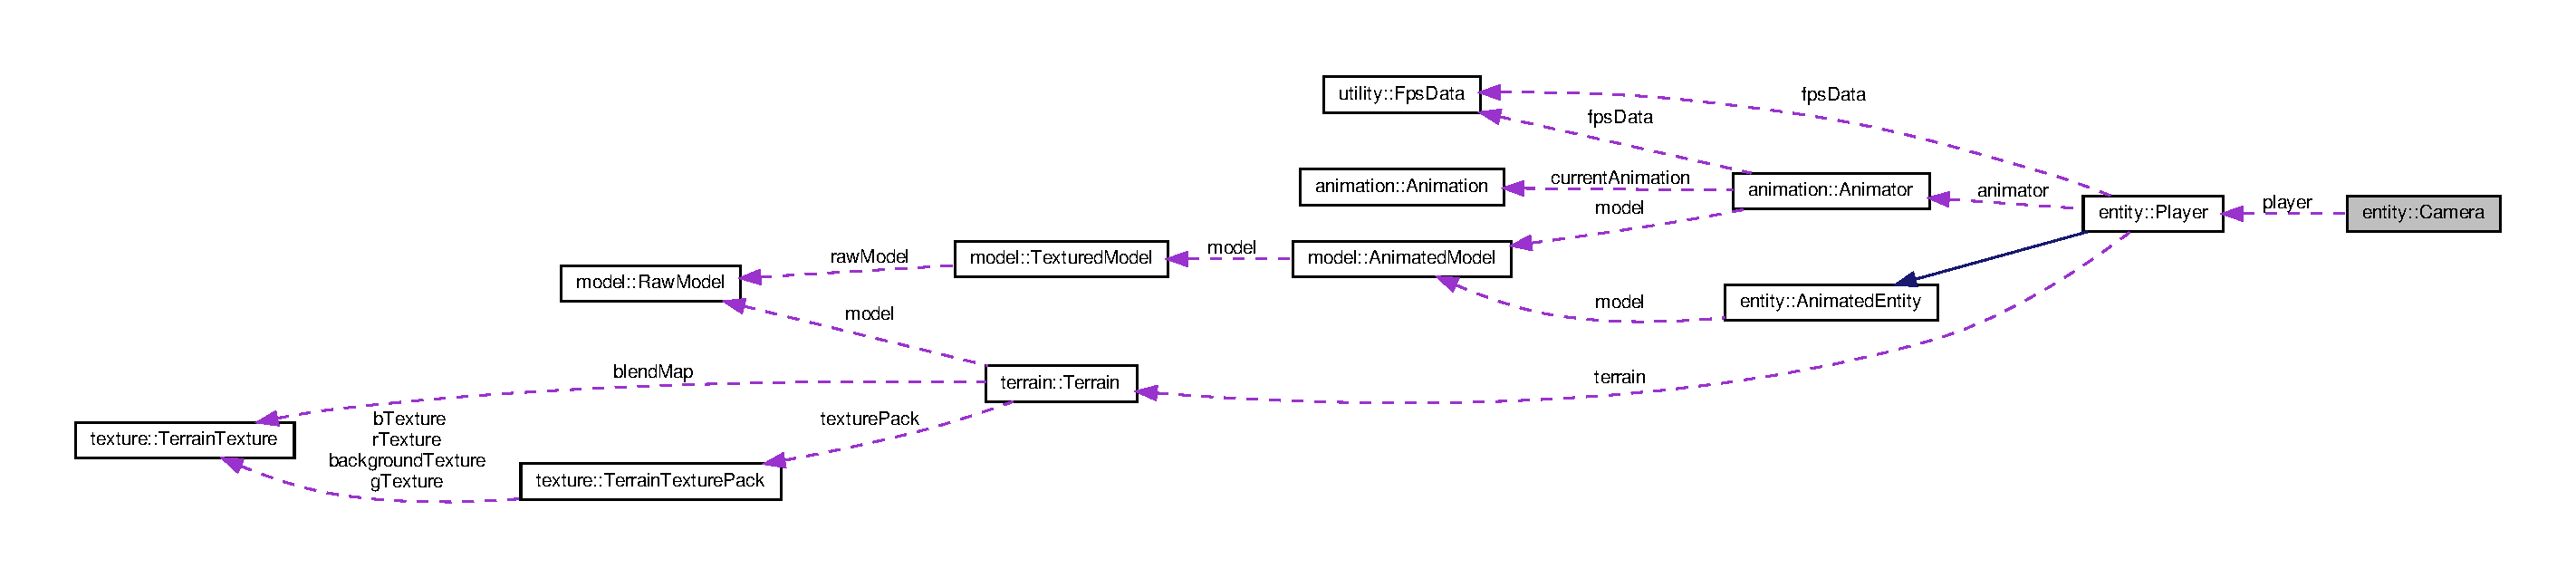
\includegraphics[width=350pt]{classentity_1_1Camera__coll__graph}
\end{center}
\end{figure}
\subsection*{Javni članovi}
\begin{DoxyCompactItemize}
\item 
\hyperlink{classentity_1_1Camera_ae28b5312d87e147f8a6a6b3f76c1d0fa}{Camera} (\hyperlink{classentity_1_1Player}{Player} $\ast$\hyperlink{classentity_1_1Camera_ace429069cf20c1138038c00b10e2c608}{player})
\begin{DoxyCompactList}\small\item\em Konstruktor klase. \end{DoxyCompactList}\item 
\hyperlink{classentity_1_1Camera_ae161d83061be4f328de222570c3ece95}{$\sim$\+Camera} ()
\begin{DoxyCompactList}\small\item\em Destruktor klase. \end{DoxyCompactList}\item 
vec3 \hyperlink{classentity_1_1Camera_a2c6b67d27b4012631306c2c2c5a3691c}{get\+Position} ()
\begin{DoxyCompactList}\small\item\em Funkcija vraca poziciju kamere. \end{DoxyCompactList}\item 
void \hyperlink{classentity_1_1Camera_a046d693a76fafe58822033c0b80bbc53}{move} ()
\begin{DoxyCompactList}\small\item\em Funkcija pomera kameru. \end{DoxyCompactList}\item 
void \hyperlink{classentity_1_1Camera_aa9a3b78671fb7385198696733b4faca4}{handle\+Mouse\+Input} (int button, int state, int x, int y)
\begin{DoxyCompactList}\small\item\em Funkcija obradjuje ulaz sa misa. \end{DoxyCompactList}\item 
void \hyperlink{classentity_1_1Camera_a04352a62ec2c4031cfde35192faf6e03}{handle\+Keyboard\+Input} (unsigned char key)
\begin{DoxyCompactList}\small\item\em Funkcija obradjuje ulaz sa tastature. Funkcija koja proverava ulaz sa tastature. \end{DoxyCompactList}\item 
float \hyperlink{classentity_1_1Camera_a502da7b4da0782356f7bf75e99e4419c}{get\+Pich} ()
\begin{DoxyCompactList}\small\item\em Funkcija vraca rotaciju oko X ose. \end{DoxyCompactList}\item 
float \hyperlink{classentity_1_1Camera_a598fc170be541c2daf281f3b3a267808}{get\+Yaw} ()
\begin{DoxyCompactList}\small\item\em Funkcija vraca rotaciju oko Y ose. \end{DoxyCompactList}\item 
float \hyperlink{classentity_1_1Camera_a9d9288cb98d6bf73c2ac749274ae3f03}{get\+Roll} ()
\begin{DoxyCompactList}\small\item\em Funkcija vraca rotaciju oko Z ose. \end{DoxyCompactList}\end{DoxyCompactItemize}
\subsection*{Privatni članovi}
\begin{DoxyCompactItemize}
\item 
void \hyperlink{classentity_1_1Camera_a7d7bed8b571309039bcfc6cbe2c829de}{calculate\+Zoom} (int button, int state)
\begin{DoxyCompactList}\small\item\em Funkcija racuna uvelicavanje pogleda. \end{DoxyCompactList}\item 
void \hyperlink{classentity_1_1Camera_a65a338e64af13f3da99b46fbf5cf879a}{calculate\+Pich} (unsigned char key)
\begin{DoxyCompactList}\small\item\em Funkcija racuna rotaciju kamere oko X ose. \end{DoxyCompactList}\item 
void \hyperlink{classentity_1_1Camera_a519f8f9f625c56a94d8860c55a134ef3}{calculate\+Angle\+Around\+Player} (unsigned char key)
\begin{DoxyCompactList}\small\item\em Funkcija racuna ugao kamere oko igraca. \end{DoxyCompactList}\item 
float \hyperlink{classentity_1_1Camera_ad5ed7dcbe9aa939d82509c23a6298251}{calculate\+Horizontal\+Distance} ()
\begin{DoxyCompactList}\small\item\em Funkcija racuna horizontalnu udaljenost od igraca. \end{DoxyCompactList}\item 
float \hyperlink{classentity_1_1Camera_a0662170fb43e41f529f4e2932a591858}{calculate\+Vertical\+Distance} ()
\begin{DoxyCompactList}\small\item\em Funkcija racuna vertikalnu udaljenost od igraca. \end{DoxyCompactList}\item 
void \hyperlink{classentity_1_1Camera_a89f1d576fd701ea58b9509b243913952}{calculate\+Camera\+Position} (float horizontal\+Distance, float vertical\+Distance)
\begin{DoxyCompactList}\small\item\em Funkcija racuna poziciju kamere. \end{DoxyCompactList}\end{DoxyCompactItemize}
\subsection*{Privatni članovi}
\begin{DoxyCompactItemize}
\item 
vec3 \hyperlink{classentity_1_1Camera_a3840344199c2da97dab4bce31d60f45e}{position}
\begin{DoxyCompactList}\small\item\em Koordinate pozicije kamere. \end{DoxyCompactList}\item 
float \hyperlink{classentity_1_1Camera_a9b05e6208aafb082a8d78d3e01d7e544}{distance\+From\+Player}
\begin{DoxyCompactList}\small\item\em Udaljenost kamere od igraca. \end{DoxyCompactList}\item 
float \hyperlink{classentity_1_1Camera_aa0d2e83177c5f3b587d030e5b8032fd2}{angle\+Around\+Player}
\begin{DoxyCompactList}\small\item\em Ugao oko igraca. \end{DoxyCompactList}\item 
float \hyperlink{classentity_1_1Camera_a33f9b55c4b44d7200e7517000fc499b2}{pich}
\begin{DoxyCompactList}\small\item\em Rotacija kamere po X osi. \end{DoxyCompactList}\item 
float \hyperlink{classentity_1_1Camera_a2ebfeecc4fe70c880813f7a4671d8b63}{yaw}
\begin{DoxyCompactList}\small\item\em Rotacija kamere po Y osi. \end{DoxyCompactList}\item 
float \hyperlink{classentity_1_1Camera_aed638e415fd894c7e39eb9fecf65afbb}{roll}
\begin{DoxyCompactList}\small\item\em Rotacija kamere po Z osi. \end{DoxyCompactList}\item 
float \hyperlink{classentity_1_1Camera_aae009950e0af66c4b5ed71f903b81513}{sensitivity}
\begin{DoxyCompactList}\small\item\em Osetljivost kamere na promene polozaja i rotacije. \end{DoxyCompactList}\item 
\hyperlink{classentity_1_1Player}{Player} $\ast$ \hyperlink{classentity_1_1Camera_ace429069cf20c1138038c00b10e2c608}{player}
\begin{DoxyCompactList}\small\item\em Pokazivac na instancu klase \hyperlink{classentity_1_1Player}{Player}. \end{DoxyCompactList}\end{DoxyCompactItemize}


\subsection{Opširniji opis}
Klasa \hyperlink{classentity_1_1Camera}{Camera} kontrolise pogled na igru. Pomocu klase \hyperlink{classentity_1_1Camera}{Camera} mozemo menjati pogled na entitete u igri kao sto je rotiranje oko objekta i uvelicavanje ili umanjivanje. 

\subsection{Dokumentacija konstruktora i destruktora}
\mbox{\Hypertarget{classentity_1_1Camera_ae28b5312d87e147f8a6a6b3f76c1d0fa}\label{classentity_1_1Camera_ae28b5312d87e147f8a6a6b3f76c1d0fa}} 
\index{entity\+::\+Camera@{entity\+::\+Camera}!Camera@{Camera}}
\index{Camera@{Camera}!entity\+::\+Camera@{entity\+::\+Camera}}
\subsubsection{\texorpdfstring{Camera()}{Camera()}}
{\footnotesize\ttfamily entity\+::\+Camera\+::\+Camera (\begin{DoxyParamCaption}\item[{\hyperlink{classentity_1_1Player}{Player} $\ast$}]{player }\end{DoxyParamCaption})}



Konstruktor klase. 


\begin{DoxyParams}{Parametri}
{\em player} & Pokazivac na instancu klase \hyperlink{classentity_1_1Player}{Player}. \\
\hline
\end{DoxyParams}
\mbox{\Hypertarget{classentity_1_1Camera_ae161d83061be4f328de222570c3ece95}\label{classentity_1_1Camera_ae161d83061be4f328de222570c3ece95}} 
\index{entity\+::\+Camera@{entity\+::\+Camera}!````~Camera@{$\sim$\+Camera}}
\index{````~Camera@{$\sim$\+Camera}!entity\+::\+Camera@{entity\+::\+Camera}}
\subsubsection{\texorpdfstring{$\sim$\+Camera()}{~Camera()}}
{\footnotesize\ttfamily entity\+::\+Camera\+::$\sim$\+Camera (\begin{DoxyParamCaption}{ }\end{DoxyParamCaption})}



Destruktor klase. 


\begin{DoxyParams}{Parametri}
{\em void} & \\
\hline
\end{DoxyParams}


\subsection{Dokumentacija funkcija članica}
\mbox{\Hypertarget{classentity_1_1Camera_a519f8f9f625c56a94d8860c55a134ef3}\label{classentity_1_1Camera_a519f8f9f625c56a94d8860c55a134ef3}} 
\index{entity\+::\+Camera@{entity\+::\+Camera}!calculate\+Angle\+Around\+Player@{calculate\+Angle\+Around\+Player}}
\index{calculate\+Angle\+Around\+Player@{calculate\+Angle\+Around\+Player}!entity\+::\+Camera@{entity\+::\+Camera}}
\subsubsection{\texorpdfstring{calculate\+Angle\+Around\+Player()}{calculateAngleAroundPlayer()}}
{\footnotesize\ttfamily void entity\+::\+Camera\+::calculate\+Angle\+Around\+Player (\begin{DoxyParamCaption}\item[{unsigned char}]{key }\end{DoxyParamCaption})\hspace{0.3cm}{\ttfamily [private]}}



Funkcija racuna ugao kamere oko igraca. 


\begin{DoxyParams}{Parametri}
{\em key} & Karakter koji je pritisnut na tastaturi \\
\hline
\end{DoxyParams}
\begin{DoxyReturn}{Vrednost funkcije}
void 
\end{DoxyReturn}
\mbox{\Hypertarget{classentity_1_1Camera_a89f1d576fd701ea58b9509b243913952}\label{classentity_1_1Camera_a89f1d576fd701ea58b9509b243913952}} 
\index{entity\+::\+Camera@{entity\+::\+Camera}!calculate\+Camera\+Position@{calculate\+Camera\+Position}}
\index{calculate\+Camera\+Position@{calculate\+Camera\+Position}!entity\+::\+Camera@{entity\+::\+Camera}}
\subsubsection{\texorpdfstring{calculate\+Camera\+Position()}{calculateCameraPosition()}}
{\footnotesize\ttfamily void entity\+::\+Camera\+::calculate\+Camera\+Position (\begin{DoxyParamCaption}\item[{float}]{horizontal\+Distance,  }\item[{float}]{vertical\+Distance }\end{DoxyParamCaption})\hspace{0.3cm}{\ttfamily [private]}}



Funkcija racuna poziciju kamere. 


\begin{DoxyParams}{Parametri}
{\em horizontal\+Distance} & Horizontalna udaljenost od igraca \\
\hline
{\em vertical\+Distance} & Vertikalna udaljenost od igraca \\
\hline
\end{DoxyParams}
\begin{DoxyReturn}{Vrednost funkcije}
void 
\end{DoxyReturn}
\mbox{\Hypertarget{classentity_1_1Camera_ad5ed7dcbe9aa939d82509c23a6298251}\label{classentity_1_1Camera_ad5ed7dcbe9aa939d82509c23a6298251}} 
\index{entity\+::\+Camera@{entity\+::\+Camera}!calculate\+Horizontal\+Distance@{calculate\+Horizontal\+Distance}}
\index{calculate\+Horizontal\+Distance@{calculate\+Horizontal\+Distance}!entity\+::\+Camera@{entity\+::\+Camera}}
\subsubsection{\texorpdfstring{calculate\+Horizontal\+Distance()}{calculateHorizontalDistance()}}
{\footnotesize\ttfamily float entity\+::\+Camera\+::calculate\+Horizontal\+Distance (\begin{DoxyParamCaption}{ }\end{DoxyParamCaption})\hspace{0.3cm}{\ttfamily [private]}}



Funkcija racuna horizontalnu udaljenost od igraca. 


\begin{DoxyParams}{Parametri}
{\em void} & \\
\hline
\end{DoxyParams}
\begin{DoxyReturn}{Vrednost funkcije}
void 
\end{DoxyReturn}
\mbox{\Hypertarget{classentity_1_1Camera_a65a338e64af13f3da99b46fbf5cf879a}\label{classentity_1_1Camera_a65a338e64af13f3da99b46fbf5cf879a}} 
\index{entity\+::\+Camera@{entity\+::\+Camera}!calculate\+Pich@{calculate\+Pich}}
\index{calculate\+Pich@{calculate\+Pich}!entity\+::\+Camera@{entity\+::\+Camera}}
\subsubsection{\texorpdfstring{calculate\+Pich()}{calculatePich()}}
{\footnotesize\ttfamily void entity\+::\+Camera\+::calculate\+Pich (\begin{DoxyParamCaption}\item[{unsigned char}]{key }\end{DoxyParamCaption})\hspace{0.3cm}{\ttfamily [private]}}



Funkcija racuna rotaciju kamere oko X ose. 


\begin{DoxyParams}{Parametri}
{\em key} & Karakter koji je pritisnut na tastaturi \\
\hline
\end{DoxyParams}
\begin{DoxyReturn}{Vrednost funkcije}
void 
\end{DoxyReturn}
\mbox{\Hypertarget{classentity_1_1Camera_a0662170fb43e41f529f4e2932a591858}\label{classentity_1_1Camera_a0662170fb43e41f529f4e2932a591858}} 
\index{entity\+::\+Camera@{entity\+::\+Camera}!calculate\+Vertical\+Distance@{calculate\+Vertical\+Distance}}
\index{calculate\+Vertical\+Distance@{calculate\+Vertical\+Distance}!entity\+::\+Camera@{entity\+::\+Camera}}
\subsubsection{\texorpdfstring{calculate\+Vertical\+Distance()}{calculateVerticalDistance()}}
{\footnotesize\ttfamily float entity\+::\+Camera\+::calculate\+Vertical\+Distance (\begin{DoxyParamCaption}{ }\end{DoxyParamCaption})\hspace{0.3cm}{\ttfamily [private]}}



Funkcija racuna vertikalnu udaljenost od igraca. 


\begin{DoxyParams}{Parametri}
{\em void} & \\
\hline
\end{DoxyParams}
\begin{DoxyReturn}{Vrednost funkcije}
void 
\end{DoxyReturn}
\mbox{\Hypertarget{classentity_1_1Camera_a7d7bed8b571309039bcfc6cbe2c829de}\label{classentity_1_1Camera_a7d7bed8b571309039bcfc6cbe2c829de}} 
\index{entity\+::\+Camera@{entity\+::\+Camera}!calculate\+Zoom@{calculate\+Zoom}}
\index{calculate\+Zoom@{calculate\+Zoom}!entity\+::\+Camera@{entity\+::\+Camera}}
\subsubsection{\texorpdfstring{calculate\+Zoom()}{calculateZoom()}}
{\footnotesize\ttfamily void entity\+::\+Camera\+::calculate\+Zoom (\begin{DoxyParamCaption}\item[{int}]{button,  }\item[{int}]{state }\end{DoxyParamCaption})\hspace{0.3cm}{\ttfamily [private]}}



Funkcija racuna uvelicavanje pogleda. 


\begin{DoxyParams}{Parametri}
{\em void} & \\
\hline
\end{DoxyParams}
\begin{DoxyReturn}{Vrednost funkcije}
void 
\end{DoxyReturn}
\mbox{\Hypertarget{classentity_1_1Camera_a502da7b4da0782356f7bf75e99e4419c}\label{classentity_1_1Camera_a502da7b4da0782356f7bf75e99e4419c}} 
\index{entity\+::\+Camera@{entity\+::\+Camera}!get\+Pich@{get\+Pich}}
\index{get\+Pich@{get\+Pich}!entity\+::\+Camera@{entity\+::\+Camera}}
\subsubsection{\texorpdfstring{get\+Pich()}{getPich()}}
{\footnotesize\ttfamily float entity\+::\+Camera\+::get\+Pich (\begin{DoxyParamCaption}{ }\end{DoxyParamCaption})}



Funkcija vraca rotaciju oko X ose. 


\begin{DoxyParams}{Parametri}
{\em void} & \\
\hline
\end{DoxyParams}
\begin{DoxyReturn}{Vrednost funkcije}
float Ugao u stepenima. 
\end{DoxyReturn}
\mbox{\Hypertarget{classentity_1_1Camera_a2c6b67d27b4012631306c2c2c5a3691c}\label{classentity_1_1Camera_a2c6b67d27b4012631306c2c2c5a3691c}} 
\index{entity\+::\+Camera@{entity\+::\+Camera}!get\+Position@{get\+Position}}
\index{get\+Position@{get\+Position}!entity\+::\+Camera@{entity\+::\+Camera}}
\subsubsection{\texorpdfstring{get\+Position()}{getPosition()}}
{\footnotesize\ttfamily vec3 entity\+::\+Camera\+::get\+Position (\begin{DoxyParamCaption}{ }\end{DoxyParamCaption})}



Funkcija vraca poziciju kamere. 


\begin{DoxyParams}{Parametri}
{\em void} & \\
\hline
\end{DoxyParams}
\begin{DoxyReturn}{Vrednost funkcije}
vec3 Vektor koji sadrzi polozaj kamere. 
\end{DoxyReturn}
\mbox{\Hypertarget{classentity_1_1Camera_a9d9288cb98d6bf73c2ac749274ae3f03}\label{classentity_1_1Camera_a9d9288cb98d6bf73c2ac749274ae3f03}} 
\index{entity\+::\+Camera@{entity\+::\+Camera}!get\+Roll@{get\+Roll}}
\index{get\+Roll@{get\+Roll}!entity\+::\+Camera@{entity\+::\+Camera}}
\subsubsection{\texorpdfstring{get\+Roll()}{getRoll()}}
{\footnotesize\ttfamily float entity\+::\+Camera\+::get\+Roll (\begin{DoxyParamCaption}{ }\end{DoxyParamCaption})}



Funkcija vraca rotaciju oko Z ose. 


\begin{DoxyParams}{Parametri}
{\em void} & \\
\hline
\end{DoxyParams}
\begin{DoxyReturn}{Vrednost funkcije}
float Ugao u stepenima. 
\end{DoxyReturn}
\mbox{\Hypertarget{classentity_1_1Camera_a598fc170be541c2daf281f3b3a267808}\label{classentity_1_1Camera_a598fc170be541c2daf281f3b3a267808}} 
\index{entity\+::\+Camera@{entity\+::\+Camera}!get\+Yaw@{get\+Yaw}}
\index{get\+Yaw@{get\+Yaw}!entity\+::\+Camera@{entity\+::\+Camera}}
\subsubsection{\texorpdfstring{get\+Yaw()}{getYaw()}}
{\footnotesize\ttfamily float entity\+::\+Camera\+::get\+Yaw (\begin{DoxyParamCaption}{ }\end{DoxyParamCaption})}



Funkcija vraca rotaciju oko Y ose. 


\begin{DoxyParams}{Parametri}
{\em void} & \\
\hline
\end{DoxyParams}
\begin{DoxyReturn}{Vrednost funkcije}
float Ugao u stepenima. 
\end{DoxyReturn}
\mbox{\Hypertarget{classentity_1_1Camera_a04352a62ec2c4031cfde35192faf6e03}\label{classentity_1_1Camera_a04352a62ec2c4031cfde35192faf6e03}} 
\index{entity\+::\+Camera@{entity\+::\+Camera}!handle\+Keyboard\+Input@{handle\+Keyboard\+Input}}
\index{handle\+Keyboard\+Input@{handle\+Keyboard\+Input}!entity\+::\+Camera@{entity\+::\+Camera}}
\subsubsection{\texorpdfstring{handle\+Keyboard\+Input()}{handleKeyboardInput()}}
{\footnotesize\ttfamily void entity\+::\+Camera\+::handle\+Keyboard\+Input (\begin{DoxyParamCaption}\item[{unsigned char}]{key }\end{DoxyParamCaption})}



Funkcija obradjuje ulaz sa tastature. Funkcija koja proverava ulaz sa tastature. 


\begin{DoxyParams}{Parametri}
{\em key} & Karakter koji je pritisnut na tastaturi \\
\hline
\end{DoxyParams}
\begin{DoxyReturn}{Vrednost funkcije}
void 
\end{DoxyReturn}
\mbox{\Hypertarget{classentity_1_1Camera_aa9a3b78671fb7385198696733b4faca4}\label{classentity_1_1Camera_aa9a3b78671fb7385198696733b4faca4}} 
\index{entity\+::\+Camera@{entity\+::\+Camera}!handle\+Mouse\+Input@{handle\+Mouse\+Input}}
\index{handle\+Mouse\+Input@{handle\+Mouse\+Input}!entity\+::\+Camera@{entity\+::\+Camera}}
\subsubsection{\texorpdfstring{handle\+Mouse\+Input()}{handleMouseInput()}}
{\footnotesize\ttfamily void entity\+::\+Camera\+::handle\+Mouse\+Input (\begin{DoxyParamCaption}\item[{int}]{button,  }\item[{int}]{state,  }\item[{int}]{x,  }\item[{int}]{y }\end{DoxyParamCaption})}



Funkcija obradjuje ulaz sa misa. 


\begin{DoxyParams}{Parametri}
{\em button} & Taster koji je pritisnut na misu \\
\hline
{\em state} & Stanje tastera(pritisnut ili otpusten) \\
\hline
{\em x} & X koordinata pozicije kursora \\
\hline
{\em y} & Y koordinata pozicije kursora \\
\hline
\end{DoxyParams}
\begin{DoxyReturn}{Vrednost funkcije}
void 
\end{DoxyReturn}
\mbox{\Hypertarget{classentity_1_1Camera_a046d693a76fafe58822033c0b80bbc53}\label{classentity_1_1Camera_a046d693a76fafe58822033c0b80bbc53}} 
\index{entity\+::\+Camera@{entity\+::\+Camera}!move@{move}}
\index{move@{move}!entity\+::\+Camera@{entity\+::\+Camera}}
\subsubsection{\texorpdfstring{move()}{move()}}
{\footnotesize\ttfamily void entity\+::\+Camera\+::move (\begin{DoxyParamCaption}{ }\end{DoxyParamCaption})}



Funkcija pomera kameru. 


\begin{DoxyParams}{Parametri}
{\em void} & \\
\hline
\end{DoxyParams}
\begin{DoxyReturn}{Vrednost funkcije}
void. 
\end{DoxyReturn}


\subsection{Dokumentacija atributa}
\mbox{\Hypertarget{classentity_1_1Camera_aa0d2e83177c5f3b587d030e5b8032fd2}\label{classentity_1_1Camera_aa0d2e83177c5f3b587d030e5b8032fd2}} 
\index{entity\+::\+Camera@{entity\+::\+Camera}!angle\+Around\+Player@{angle\+Around\+Player}}
\index{angle\+Around\+Player@{angle\+Around\+Player}!entity\+::\+Camera@{entity\+::\+Camera}}
\subsubsection{\texorpdfstring{angle\+Around\+Player}{angleAroundPlayer}}
{\footnotesize\ttfamily float entity\+::\+Camera\+::angle\+Around\+Player\hspace{0.3cm}{\ttfamily [private]}}



Ugao oko igraca. 

\mbox{\Hypertarget{classentity_1_1Camera_a9b05e6208aafb082a8d78d3e01d7e544}\label{classentity_1_1Camera_a9b05e6208aafb082a8d78d3e01d7e544}} 
\index{entity\+::\+Camera@{entity\+::\+Camera}!distance\+From\+Player@{distance\+From\+Player}}
\index{distance\+From\+Player@{distance\+From\+Player}!entity\+::\+Camera@{entity\+::\+Camera}}
\subsubsection{\texorpdfstring{distance\+From\+Player}{distanceFromPlayer}}
{\footnotesize\ttfamily float entity\+::\+Camera\+::distance\+From\+Player\hspace{0.3cm}{\ttfamily [private]}}



Udaljenost kamere od igraca. 

\mbox{\Hypertarget{classentity_1_1Camera_a33f9b55c4b44d7200e7517000fc499b2}\label{classentity_1_1Camera_a33f9b55c4b44d7200e7517000fc499b2}} 
\index{entity\+::\+Camera@{entity\+::\+Camera}!pich@{pich}}
\index{pich@{pich}!entity\+::\+Camera@{entity\+::\+Camera}}
\subsubsection{\texorpdfstring{pich}{pich}}
{\footnotesize\ttfamily float entity\+::\+Camera\+::pich\hspace{0.3cm}{\ttfamily [private]}}



Rotacija kamere po X osi. 

\mbox{\Hypertarget{classentity_1_1Camera_ace429069cf20c1138038c00b10e2c608}\label{classentity_1_1Camera_ace429069cf20c1138038c00b10e2c608}} 
\index{entity\+::\+Camera@{entity\+::\+Camera}!player@{player}}
\index{player@{player}!entity\+::\+Camera@{entity\+::\+Camera}}
\subsubsection{\texorpdfstring{player}{player}}
{\footnotesize\ttfamily \hyperlink{classentity_1_1Player}{Player}$\ast$ entity\+::\+Camera\+::player\hspace{0.3cm}{\ttfamily [private]}}



Pokazivac na instancu klase \hyperlink{classentity_1_1Player}{Player}. 

\mbox{\Hypertarget{classentity_1_1Camera_a3840344199c2da97dab4bce31d60f45e}\label{classentity_1_1Camera_a3840344199c2da97dab4bce31d60f45e}} 
\index{entity\+::\+Camera@{entity\+::\+Camera}!position@{position}}
\index{position@{position}!entity\+::\+Camera@{entity\+::\+Camera}}
\subsubsection{\texorpdfstring{position}{position}}
{\footnotesize\ttfamily vec3 entity\+::\+Camera\+::position\hspace{0.3cm}{\ttfamily [private]}}



Koordinate pozicije kamere. 

\mbox{\Hypertarget{classentity_1_1Camera_aed638e415fd894c7e39eb9fecf65afbb}\label{classentity_1_1Camera_aed638e415fd894c7e39eb9fecf65afbb}} 
\index{entity\+::\+Camera@{entity\+::\+Camera}!roll@{roll}}
\index{roll@{roll}!entity\+::\+Camera@{entity\+::\+Camera}}
\subsubsection{\texorpdfstring{roll}{roll}}
{\footnotesize\ttfamily float entity\+::\+Camera\+::roll\hspace{0.3cm}{\ttfamily [private]}}



Rotacija kamere po Z osi. 

\mbox{\Hypertarget{classentity_1_1Camera_aae009950e0af66c4b5ed71f903b81513}\label{classentity_1_1Camera_aae009950e0af66c4b5ed71f903b81513}} 
\index{entity\+::\+Camera@{entity\+::\+Camera}!sensitivity@{sensitivity}}
\index{sensitivity@{sensitivity}!entity\+::\+Camera@{entity\+::\+Camera}}
\subsubsection{\texorpdfstring{sensitivity}{sensitivity}}
{\footnotesize\ttfamily float entity\+::\+Camera\+::sensitivity\hspace{0.3cm}{\ttfamily [private]}}



Osetljivost kamere na promene polozaja i rotacije. 

\mbox{\Hypertarget{classentity_1_1Camera_a2ebfeecc4fe70c880813f7a4671d8b63}\label{classentity_1_1Camera_a2ebfeecc4fe70c880813f7a4671d8b63}} 
\index{entity\+::\+Camera@{entity\+::\+Camera}!yaw@{yaw}}
\index{yaw@{yaw}!entity\+::\+Camera@{entity\+::\+Camera}}
\subsubsection{\texorpdfstring{yaw}{yaw}}
{\footnotesize\ttfamily float entity\+::\+Camera\+::yaw\hspace{0.3cm}{\ttfamily [private]}}



Rotacija kamere po Y osi. 



Dokumentacija ove klase je napravljena na osnovu sledećih datoteka\+:\begin{DoxyCompactItemize}
\item 
/home/dusan/\+Documents/\+R\+G146-\/vitez-\/reda-\/zmaja/include/entity/\hyperlink{Camera_8h}{Camera.\+h}\item 
/home/dusan/\+Documents/\+R\+G146-\/vitez-\/reda-\/zmaja/src/entity/\hyperlink{Camera_8cpp}{Camera.\+cpp}\end{DoxyCompactItemize}

\hypertarget{classcore_1_1Engine}{}\section{Dokumentacija klase core\+:\+:Engine}
\label{classcore_1_1Engine}\index{core\+::\+Engine@{core\+::\+Engine}}


Klasa \hyperlink{classcore_1_1Engine}{Engine} je jezgro i kontroler programa. Sva bitnija podesavanja i inicijalizacije desavaju se u ovoj klasi. Klasa je zaduzena za inicijalizaciju G\+L\+U\+T-\/a , Open\+G\+L-\/a, i kontrolisanje i kreiranje ostalih korisnicki definisanih klasa i funkcija.  




{\ttfamily \#include $<$Engine.\+h$>$}

\subsection*{Javni članovi}
\begin{DoxyCompactItemize}
\item 
\hyperlink{classcore_1_1Engine_adcfd692be68f28117c7234ae09fd0824}{Engine} ()
\begin{DoxyCompactList}\small\item\em Konstruktor klase. \end{DoxyCompactList}\item 
\hyperlink{classcore_1_1Engine_afadff2634c914c9f6c4ade95e78ff693}{$\sim$\+Engine} ()
\begin{DoxyCompactList}\small\item\em Destruktor klase. \end{DoxyCompactList}\item 
void \hyperlink{classcore_1_1Engine_ac0cb11890396ccdf5100bc73045c4d38}{start} (int $\ast$argcp, char $\ast$$\ast$argv)
\begin{DoxyCompactList}\small\item\em Funkcija startuje bitne procese za funkcionisanje. U funkciji se pozivaju funkcije za inicijalizaciju G\+L\+U\+T-\/a, Opnen\+G\+L-\/a, funkcija za kreiranje prozora i registraciju callback funkcija. Takodje funkcija pokrece glavnu petlju programa. \end{DoxyCompactList}\end{DoxyCompactItemize}
\subsection*{Privatni članovi}
\begin{DoxyCompactItemize}
\item 
void \hyperlink{classcore_1_1Engine_a737de95b00aa5b62c466f2e3dc4edcdb}{init\+Glut} (int $\ast$argcp, char $\ast$$\ast$argv)
\begin{DoxyCompactList}\small\item\em Funkcija inicijalizuje G\+L\+UT. U funkciji se postavljalju parametri osnovnih funkcija za inicijalizaciju G\+L\+U\+T-\/a. \end{DoxyCompactList}\item 
void \hyperlink{classcore_1_1Engine_ad6d0e175eff6ec04d3e5af53a78443ef}{create\+Window} (void)
\begin{DoxyCompactList}\small\item\em Funkcija kreira prozor na racunaru. U funkciji se postavljalju parametri prozora kao sto su ime prozora, sirini i visina , i pozicija. Parametri su definisani kao lokalne promenljive klase. \end{DoxyCompactList}\item 
void \hyperlink{classcore_1_1Engine_a6cfe680acf87f9882f92b1ffc134021f}{init\+Gl} (void)
\begin{DoxyCompactList}\small\item\em Funkcija inicijalizuje Open\+GL. U funkciji se postavjalju parametri osnovnih Open\+GL funkcija, takodje se unutar funkcije ucitavaju modeli i informacije koje je potrebno ucitati pre glavne petlje programa. \end{DoxyCompactList}\item 
void \hyperlink{classcore_1_1Engine_a4a8c96ce1172195507d2233479837ad2}{register\+Callback\+Functions} (void)
\begin{DoxyCompactList}\small\item\em Funkcija registruje callback funkcije. U funkciji se pomocu G\+L\+UT funkcija prosledjuju pokazivaci callback funkcija. \end{DoxyCompactList}\end{DoxyCompactItemize}


\subsection{Opširniji opis}
Klasa \hyperlink{classcore_1_1Engine}{Engine} je jezgro i kontroler programa. Sva bitnija podesavanja i inicijalizacije desavaju se u ovoj klasi. Klasa je zaduzena za inicijalizaciju G\+L\+U\+T-\/a , Open\+G\+L-\/a, i kontrolisanje i kreiranje ostalih korisnicki definisanih klasa i funkcija. 

\subsection{Dokumentacija konstruktora i destruktora}
\mbox{\Hypertarget{classcore_1_1Engine_adcfd692be68f28117c7234ae09fd0824}\label{classcore_1_1Engine_adcfd692be68f28117c7234ae09fd0824}} 
\index{core\+::\+Engine@{core\+::\+Engine}!Engine@{Engine}}
\index{Engine@{Engine}!core\+::\+Engine@{core\+::\+Engine}}
\subsubsection{\texorpdfstring{Engine()}{Engine()}}
{\footnotesize\ttfamily core\+::\+Engine\+::\+Engine (\begin{DoxyParamCaption}{ }\end{DoxyParamCaption})}



Konstruktor klase. 


\begin{DoxyParams}{Parametri}
{\em void} & \\
\hline
\end{DoxyParams}
\mbox{\Hypertarget{classcore_1_1Engine_afadff2634c914c9f6c4ade95e78ff693}\label{classcore_1_1Engine_afadff2634c914c9f6c4ade95e78ff693}} 
\index{core\+::\+Engine@{core\+::\+Engine}!````~Engine@{$\sim$\+Engine}}
\index{````~Engine@{$\sim$\+Engine}!core\+::\+Engine@{core\+::\+Engine}}
\subsubsection{\texorpdfstring{$\sim$\+Engine()}{~Engine()}}
{\footnotesize\ttfamily core\+::\+Engine\+::$\sim$\+Engine (\begin{DoxyParamCaption}{ }\end{DoxyParamCaption})}



Destruktor klase. 


\begin{DoxyParams}{Parametri}
{\em void} & \\
\hline
\end{DoxyParams}


\subsection{Dokumentacija funkcija članica}
\mbox{\Hypertarget{classcore_1_1Engine_ad6d0e175eff6ec04d3e5af53a78443ef}\label{classcore_1_1Engine_ad6d0e175eff6ec04d3e5af53a78443ef}} 
\index{core\+::\+Engine@{core\+::\+Engine}!create\+Window@{create\+Window}}
\index{create\+Window@{create\+Window}!core\+::\+Engine@{core\+::\+Engine}}
\subsubsection{\texorpdfstring{create\+Window()}{createWindow()}}
{\footnotesize\ttfamily void core\+::\+Engine\+::create\+Window (\begin{DoxyParamCaption}\item[{void}]{ }\end{DoxyParamCaption})\hspace{0.3cm}{\ttfamily [private]}}



Funkcija kreira prozor na racunaru. U funkciji se postavljalju parametri prozora kao sto su ime prozora, sirini i visina , i pozicija. Parametri su definisani kao lokalne promenljive klase. 


\begin{DoxyParams}{Parametri}
{\em void} & \\
\hline
\end{DoxyParams}
\begin{DoxyReturn}{Vrednost funkcije}
void 
\end{DoxyReturn}
\mbox{\Hypertarget{classcore_1_1Engine_a6cfe680acf87f9882f92b1ffc134021f}\label{classcore_1_1Engine_a6cfe680acf87f9882f92b1ffc134021f}} 
\index{core\+::\+Engine@{core\+::\+Engine}!init\+Gl@{init\+Gl}}
\index{init\+Gl@{init\+Gl}!core\+::\+Engine@{core\+::\+Engine}}
\subsubsection{\texorpdfstring{init\+Gl()}{initGl()}}
{\footnotesize\ttfamily void core\+::\+Engine\+::init\+Gl (\begin{DoxyParamCaption}\item[{void}]{ }\end{DoxyParamCaption})\hspace{0.3cm}{\ttfamily [private]}}



Funkcija inicijalizuje Open\+GL. U funkciji se postavjalju parametri osnovnih Open\+GL funkcija, takodje se unutar funkcije ucitavaju modeli i informacije koje je potrebno ucitati pre glavne petlje programa. 


\begin{DoxyParams}{Parametri}
{\em void} & \\
\hline
\end{DoxyParams}
\begin{DoxyReturn}{Vrednost funkcije}
void 
\end{DoxyReturn}
\mbox{\Hypertarget{classcore_1_1Engine_a737de95b00aa5b62c466f2e3dc4edcdb}\label{classcore_1_1Engine_a737de95b00aa5b62c466f2e3dc4edcdb}} 
\index{core\+::\+Engine@{core\+::\+Engine}!init\+Glut@{init\+Glut}}
\index{init\+Glut@{init\+Glut}!core\+::\+Engine@{core\+::\+Engine}}
\subsubsection{\texorpdfstring{init\+Glut()}{initGlut()}}
{\footnotesize\ttfamily void core\+::\+Engine\+::init\+Glut (\begin{DoxyParamCaption}\item[{int $\ast$}]{argcp,  }\item[{char $\ast$$\ast$}]{argv }\end{DoxyParamCaption})\hspace{0.3cm}{\ttfamily [private]}}



Funkcija inicijalizuje G\+L\+UT. U funkciji se postavljalju parametri osnovnih funkcija za inicijalizaciju G\+L\+U\+T-\/a. 


\begin{DoxyParams}{Parametri}
{\em argcp} & Pokazivac na broj argumenata programa \\
\hline
{\em argv} & Niz niski koje su argumenti programa \\
\hline
\end{DoxyParams}
\begin{DoxyReturn}{Vrednost funkcije}
void 
\end{DoxyReturn}
\mbox{\Hypertarget{classcore_1_1Engine_a4a8c96ce1172195507d2233479837ad2}\label{classcore_1_1Engine_a4a8c96ce1172195507d2233479837ad2}} 
\index{core\+::\+Engine@{core\+::\+Engine}!register\+Callback\+Functions@{register\+Callback\+Functions}}
\index{register\+Callback\+Functions@{register\+Callback\+Functions}!core\+::\+Engine@{core\+::\+Engine}}
\subsubsection{\texorpdfstring{register\+Callback\+Functions()}{registerCallbackFunctions()}}
{\footnotesize\ttfamily void core\+::\+Engine\+::register\+Callback\+Functions (\begin{DoxyParamCaption}\item[{void}]{ }\end{DoxyParamCaption})\hspace{0.3cm}{\ttfamily [private]}}



Funkcija registruje callback funkcije. U funkciji se pomocu G\+L\+UT funkcija prosledjuju pokazivaci callback funkcija. 


\begin{DoxyParams}{Parametri}
{\em void} & \\
\hline
\end{DoxyParams}
\begin{DoxyReturn}{Vrednost funkcije}
void 
\end{DoxyReturn}
\mbox{\Hypertarget{classcore_1_1Engine_ac0cb11890396ccdf5100bc73045c4d38}\label{classcore_1_1Engine_ac0cb11890396ccdf5100bc73045c4d38}} 
\index{core\+::\+Engine@{core\+::\+Engine}!start@{start}}
\index{start@{start}!core\+::\+Engine@{core\+::\+Engine}}
\subsubsection{\texorpdfstring{start()}{start()}}
{\footnotesize\ttfamily void core\+::\+Engine\+::start (\begin{DoxyParamCaption}\item[{int $\ast$}]{argcp,  }\item[{char $\ast$$\ast$}]{argv }\end{DoxyParamCaption})}



Funkcija startuje bitne procese za funkcionisanje. U funkciji se pozivaju funkcije za inicijalizaciju G\+L\+U\+T-\/a, Opnen\+G\+L-\/a, funkcija za kreiranje prozora i registraciju callback funkcija. Takodje funkcija pokrece glavnu petlju programa. 


\begin{DoxyParams}{Parametri}
{\em argcp} & Pokazivac na broj argumenata programa \\
\hline
{\em argv} & Niz niski koje su argumenti programa \\
\hline
\end{DoxyParams}
\begin{DoxyReturn}{Vrednost funkcije}
void 
\end{DoxyReturn}


Dokumentacija ove klase je napravljena na osnovu sledećih datoteka\+:\begin{DoxyCompactItemize}
\item 
/home/dusan/\+Documents/\+R\+G146-\/vitez-\/reda-\/zmaja/include/core/\hyperlink{Engine_8h}{Engine.\+h}\item 
/home/dusan/\+Documents/\+R\+G146-\/vitez-\/reda-\/zmaja/src/core/\hyperlink{Engine_8cpp}{Engine.\+cpp}\end{DoxyCompactItemize}

\hypertarget{classentity_1_1Entity}{}\section{Dokumentacija klase entity\+:\+:Entity}
\label{classentity_1_1Entity}\index{entity\+::\+Entity@{entity\+::\+Entity}}


Klasa \hyperlink{classentity_1_1Entity}{Entity} odredjuje jedan entitet. Pomocu klase \hyperlink{classentity_1_1Entity}{Entity} odredjujemo entitet tako sto mu pridruzujemo teksturisan model kao i poziciju u svetu i ostale transformacije.  




{\ttfamily \#include $<$Entity.\+h$>$}



Dijagram nasleđivanja za klasu entity\+:\+:Entity\+:\nopagebreak
\begin{figure}[H]
\begin{center}
\leavevmode
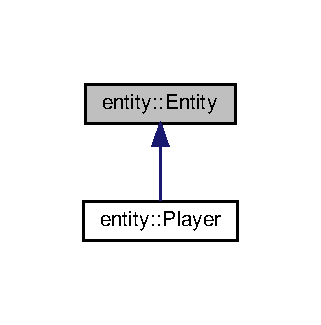
\includegraphics[width=154pt]{classentity_1_1Entity__inherit__graph}
\end{center}
\end{figure}


Klasni dijagram za entity\+:\+:Entity\+:\nopagebreak
\begin{figure}[H]
\begin{center}
\leavevmode
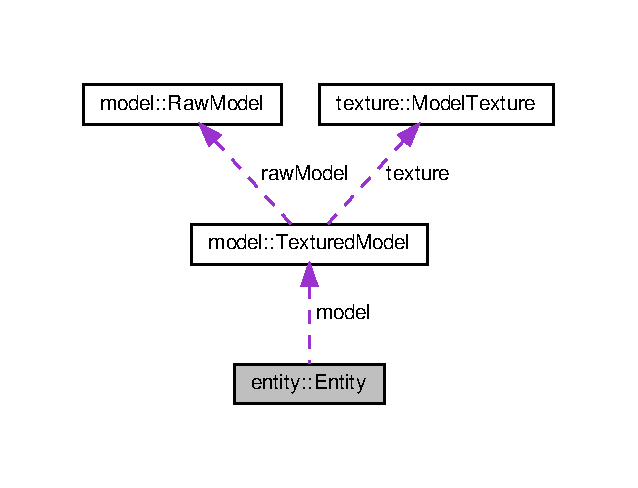
\includegraphics[width=306pt]{classentity_1_1Entity__coll__graph}
\end{center}
\end{figure}
\subsection*{Javni članovi}
\begin{DoxyCompactItemize}
\item 
\hyperlink{classentity_1_1Entity_a1668042c968a630c82bbbcec8520400e}{Entity} (\hyperlink{classmodel_1_1TexturedModel}{Textured\+Model} $\ast$\hyperlink{classentity_1_1Entity_ac7848c5d47d4b2bf12c84ddbbc32052a}{model}, vec3 \hyperlink{classentity_1_1Entity_ad409c7f2085024479b276c2b6948bddb}{position}, vec3 \hyperlink{classentity_1_1Entity_aedb4c5dc1cfbc8cb3f6deb565ea920cb}{rotation}, float \hyperlink{classentity_1_1Entity_a59e5d5e3575df70cd5c74b5d739d84ca}{scale})
\begin{DoxyCompactList}\small\item\em Konstruktor klase. \end{DoxyCompactList}\item 
\hyperlink{classentity_1_1Entity_a2d1aa154095b15e2dd6fa484ec00867e}{$\sim$\+Entity} ()
\begin{DoxyCompactList}\small\item\em Destruktor klase. \end{DoxyCompactList}\item 
\hyperlink{classmodel_1_1TexturedModel}{Textured\+Model} $\ast$ \hyperlink{classentity_1_1Entity_abc6481a8bab918cfb1309d3d342ccad1}{get\+Model} ()
\begin{DoxyCompactList}\small\item\em Funkcija vraca texturisan model. \end{DoxyCompactList}\item 
void \hyperlink{classentity_1_1Entity_a68bdcd0dcae978514e87ee53c60367e2}{set\+Model} (\hyperlink{classmodel_1_1TexturedModel}{Textured\+Model} $\ast$\hyperlink{classentity_1_1Entity_ac7848c5d47d4b2bf12c84ddbbc32052a}{model})
\begin{DoxyCompactList}\small\item\em Funkcija postavlja texturisan model. \end{DoxyCompactList}\item 
vec3 \hyperlink{classentity_1_1Entity_ad255abb1afcceceb6f2efea66086d8bd}{get\+Position} ()
\begin{DoxyCompactList}\small\item\em Funkcija vraca poziciju entiteta. \end{DoxyCompactList}\item 
void \hyperlink{classentity_1_1Entity_abb5f477d3eac07d19f0545df10e3077c}{set\+Position} (vec3 \hyperlink{classentity_1_1Entity_ad409c7f2085024479b276c2b6948bddb}{position})
\begin{DoxyCompactList}\small\item\em Funkcija postavlja poziciju entiteta. \end{DoxyCompactList}\item 
vec3 \hyperlink{classentity_1_1Entity_a58680b88c9179d9cab22e881b320f9f7}{get\+Rotation} ()
\begin{DoxyCompactList}\small\item\em Funkcija vraca rotaciju entiteta. \end{DoxyCompactList}\item 
void \hyperlink{classentity_1_1Entity_a830cb1b8769d11322844a34f1e480e4b}{set\+Rotation} (vec3 \hyperlink{classentity_1_1Entity_aedb4c5dc1cfbc8cb3f6deb565ea920cb}{rotation})
\begin{DoxyCompactList}\small\item\em Funkcija postavlja rotaciju entiteta. \end{DoxyCompactList}\item 
float \hyperlink{classentity_1_1Entity_a1923a9ecf9da2ec77d6e3eeadb4bd4d7}{get\+Scale} ()
\begin{DoxyCompactList}\small\item\em Funkcija vraca skaliranje entiteta. \end{DoxyCompactList}\item 
void \hyperlink{classentity_1_1Entity_a5d2d7bd6cd754ce566e2d4a9e4b991e0}{set\+Scale} (float \hyperlink{classentity_1_1Entity_a59e5d5e3575df70cd5c74b5d739d84ca}{scale})
\begin{DoxyCompactList}\small\item\em Funkcija postavlja skaliranje entiteta. \end{DoxyCompactList}\item 
void \hyperlink{classentity_1_1Entity_a24a22a1554a3a412cc2583bbf87fd77c}{increase\+Position} (vec3 delta\+Position)
\begin{DoxyCompactList}\small\item\em Funkcija povecava poziciju entiteta. \end{DoxyCompactList}\item 
void \hyperlink{classentity_1_1Entity_ac5bd766ea7810db89b8948160916768a}{increase\+Rotation} (vec3 delta\+Rotation)
\begin{DoxyCompactList}\small\item\em Funkcija povecava rotaciju entiteta. \end{DoxyCompactList}\end{DoxyCompactItemize}
\subsection*{Privatni članovi}
\begin{DoxyCompactItemize}
\item 
\hyperlink{classmodel_1_1TexturedModel}{Textured\+Model} $\ast$ \hyperlink{classentity_1_1Entity_ac7848c5d47d4b2bf12c84ddbbc32052a}{model}
\begin{DoxyCompactList}\small\item\em Pokazivac na instancu klase Textured\+Model. \end{DoxyCompactList}\item 
vec3 \hyperlink{classentity_1_1Entity_ad409c7f2085024479b276c2b6948bddb}{position}
\begin{DoxyCompactList}\small\item\em Pozicija entiteta. \end{DoxyCompactList}\item 
vec3 \hyperlink{classentity_1_1Entity_aedb4c5dc1cfbc8cb3f6deb565ea920cb}{rotation}
\begin{DoxyCompactList}\small\item\em Rotacija entiteta. \end{DoxyCompactList}\item 
float \hyperlink{classentity_1_1Entity_a59e5d5e3575df70cd5c74b5d739d84ca}{scale}
\begin{DoxyCompactList}\small\item\em Skaliranje entiteta. \end{DoxyCompactList}\end{DoxyCompactItemize}


\subsection{Opširniji opis}
Klasa \hyperlink{classentity_1_1Entity}{Entity} odredjuje jedan entitet. Pomocu klase \hyperlink{classentity_1_1Entity}{Entity} odredjujemo entitet tako sto mu pridruzujemo teksturisan model kao i poziciju u svetu i ostale transformacije. 

\subsection{Dokumentacija konstruktora i destruktora}
\mbox{\Hypertarget{classentity_1_1Entity_a1668042c968a630c82bbbcec8520400e}\label{classentity_1_1Entity_a1668042c968a630c82bbbcec8520400e}} 
\index{entity\+::\+Entity@{entity\+::\+Entity}!Entity@{Entity}}
\index{Entity@{Entity}!entity\+::\+Entity@{entity\+::\+Entity}}
\subsubsection{\texorpdfstring{Entity()}{Entity()}}
{\footnotesize\ttfamily entity\+::\+Entity\+::\+Entity (\begin{DoxyParamCaption}\item[{\hyperlink{classmodel_1_1TexturedModel}{Textured\+Model} $\ast$}]{model,  }\item[{vec3}]{position,  }\item[{vec3}]{rotation,  }\item[{float}]{scale }\end{DoxyParamCaption})}



Konstruktor klase. 


\begin{DoxyParams}{Parametri}
{\em model} & Pokazivac na instancu klase Textured\+Model. \\
\hline
{\em position} & Pozicija entiteta. \\
\hline
{\em rotation} & Rotacija entiteta. \\
\hline
{\em scale} & Skaliranje entiteta. \\
\hline
\end{DoxyParams}
\mbox{\Hypertarget{classentity_1_1Entity_a2d1aa154095b15e2dd6fa484ec00867e}\label{classentity_1_1Entity_a2d1aa154095b15e2dd6fa484ec00867e}} 
\index{entity\+::\+Entity@{entity\+::\+Entity}!````~Entity@{$\sim$\+Entity}}
\index{````~Entity@{$\sim$\+Entity}!entity\+::\+Entity@{entity\+::\+Entity}}
\subsubsection{\texorpdfstring{$\sim$\+Entity()}{~Entity()}}
{\footnotesize\ttfamily entity\+::\+Entity\+::$\sim$\+Entity (\begin{DoxyParamCaption}{ }\end{DoxyParamCaption})}



Destruktor klase. 


\begin{DoxyParams}{Parametri}
{\em void} & \\
\hline
\end{DoxyParams}


\subsection{Dokumentacija funkcija članica}
\mbox{\Hypertarget{classentity_1_1Entity_abc6481a8bab918cfb1309d3d342ccad1}\label{classentity_1_1Entity_abc6481a8bab918cfb1309d3d342ccad1}} 
\index{entity\+::\+Entity@{entity\+::\+Entity}!get\+Model@{get\+Model}}
\index{get\+Model@{get\+Model}!entity\+::\+Entity@{entity\+::\+Entity}}
\subsubsection{\texorpdfstring{get\+Model()}{getModel()}}
{\footnotesize\ttfamily \hyperlink{classmodel_1_1TexturedModel}{Textured\+Model} $\ast$ entity\+::\+Entity\+::get\+Model (\begin{DoxyParamCaption}{ }\end{DoxyParamCaption})}



Funkcija vraca texturisan model. 


\begin{DoxyParams}{Parametri}
{\em void} & \\
\hline
\end{DoxyParams}
\begin{DoxyReturn}{Vrednost funkcije}
Textured\+Model $\ast$ Pokazivac na instancu klase Textured\+Model. 
\end{DoxyReturn}
\mbox{\Hypertarget{classentity_1_1Entity_ad255abb1afcceceb6f2efea66086d8bd}\label{classentity_1_1Entity_ad255abb1afcceceb6f2efea66086d8bd}} 
\index{entity\+::\+Entity@{entity\+::\+Entity}!get\+Position@{get\+Position}}
\index{get\+Position@{get\+Position}!entity\+::\+Entity@{entity\+::\+Entity}}
\subsubsection{\texorpdfstring{get\+Position()}{getPosition()}}
{\footnotesize\ttfamily vec3 entity\+::\+Entity\+::get\+Position (\begin{DoxyParamCaption}{ }\end{DoxyParamCaption})}



Funkcija vraca poziciju entiteta. 


\begin{DoxyParams}{Parametri}
{\em void} & \\
\hline
\end{DoxyParams}
\begin{DoxyReturn}{Vrednost funkcije}
vec3 Pozicija entiteta. 
\end{DoxyReturn}
\mbox{\Hypertarget{classentity_1_1Entity_a58680b88c9179d9cab22e881b320f9f7}\label{classentity_1_1Entity_a58680b88c9179d9cab22e881b320f9f7}} 
\index{entity\+::\+Entity@{entity\+::\+Entity}!get\+Rotation@{get\+Rotation}}
\index{get\+Rotation@{get\+Rotation}!entity\+::\+Entity@{entity\+::\+Entity}}
\subsubsection{\texorpdfstring{get\+Rotation()}{getRotation()}}
{\footnotesize\ttfamily vec3 entity\+::\+Entity\+::get\+Rotation (\begin{DoxyParamCaption}{ }\end{DoxyParamCaption})}



Funkcija vraca rotaciju entiteta. 


\begin{DoxyParams}{Parametri}
{\em void} & \\
\hline
\end{DoxyParams}
\begin{DoxyReturn}{Vrednost funkcije}
vec3 Rotacija entiteta. 
\end{DoxyReturn}
\mbox{\Hypertarget{classentity_1_1Entity_a1923a9ecf9da2ec77d6e3eeadb4bd4d7}\label{classentity_1_1Entity_a1923a9ecf9da2ec77d6e3eeadb4bd4d7}} 
\index{entity\+::\+Entity@{entity\+::\+Entity}!get\+Scale@{get\+Scale}}
\index{get\+Scale@{get\+Scale}!entity\+::\+Entity@{entity\+::\+Entity}}
\subsubsection{\texorpdfstring{get\+Scale()}{getScale()}}
{\footnotesize\ttfamily float entity\+::\+Entity\+::get\+Scale (\begin{DoxyParamCaption}{ }\end{DoxyParamCaption})}



Funkcija vraca skaliranje entiteta. 


\begin{DoxyParams}{Parametri}
{\em void} & \\
\hline
\end{DoxyParams}
\begin{DoxyReturn}{Vrednost funkcije}
float Skaliranje entiteta. 
\end{DoxyReturn}
\mbox{\Hypertarget{classentity_1_1Entity_a24a22a1554a3a412cc2583bbf87fd77c}\label{classentity_1_1Entity_a24a22a1554a3a412cc2583bbf87fd77c}} 
\index{entity\+::\+Entity@{entity\+::\+Entity}!increase\+Position@{increase\+Position}}
\index{increase\+Position@{increase\+Position}!entity\+::\+Entity@{entity\+::\+Entity}}
\subsubsection{\texorpdfstring{increase\+Position()}{increasePosition()}}
{\footnotesize\ttfamily void entity\+::\+Entity\+::increase\+Position (\begin{DoxyParamCaption}\item[{vec3}]{delta\+Position }\end{DoxyParamCaption})}



Funkcija povecava poziciju entiteta. 


\begin{DoxyParams}{Parametri}
{\em delta\+Position} & Pozicija entiteta. \\
\hline
\end{DoxyParams}
\begin{DoxyReturn}{Vrednost funkcije}
void 
\end{DoxyReturn}
\mbox{\Hypertarget{classentity_1_1Entity_ac5bd766ea7810db89b8948160916768a}\label{classentity_1_1Entity_ac5bd766ea7810db89b8948160916768a}} 
\index{entity\+::\+Entity@{entity\+::\+Entity}!increase\+Rotation@{increase\+Rotation}}
\index{increase\+Rotation@{increase\+Rotation}!entity\+::\+Entity@{entity\+::\+Entity}}
\subsubsection{\texorpdfstring{increase\+Rotation()}{increaseRotation()}}
{\footnotesize\ttfamily void entity\+::\+Entity\+::increase\+Rotation (\begin{DoxyParamCaption}\item[{vec3}]{delta\+Rotation }\end{DoxyParamCaption})}



Funkcija povecava rotaciju entiteta. 


\begin{DoxyParams}{Parametri}
{\em delta\+Rotation} & Rotacija entiteta. \\
\hline
\end{DoxyParams}
\begin{DoxyReturn}{Vrednost funkcije}
void 
\end{DoxyReturn}
\mbox{\Hypertarget{classentity_1_1Entity_a68bdcd0dcae978514e87ee53c60367e2}\label{classentity_1_1Entity_a68bdcd0dcae978514e87ee53c60367e2}} 
\index{entity\+::\+Entity@{entity\+::\+Entity}!set\+Model@{set\+Model}}
\index{set\+Model@{set\+Model}!entity\+::\+Entity@{entity\+::\+Entity}}
\subsubsection{\texorpdfstring{set\+Model()}{setModel()}}
{\footnotesize\ttfamily void entity\+::\+Entity\+::set\+Model (\begin{DoxyParamCaption}\item[{\hyperlink{classmodel_1_1TexturedModel}{Textured\+Model} $\ast$}]{model }\end{DoxyParamCaption})}



Funkcija postavlja texturisan model. 


\begin{DoxyParams}{Parametri}
{\em model} & Pokazivac na instancu klase Textured\+Model. \\
\hline
\end{DoxyParams}
\begin{DoxyReturn}{Vrednost funkcije}
void 
\end{DoxyReturn}
\mbox{\Hypertarget{classentity_1_1Entity_abb5f477d3eac07d19f0545df10e3077c}\label{classentity_1_1Entity_abb5f477d3eac07d19f0545df10e3077c}} 
\index{entity\+::\+Entity@{entity\+::\+Entity}!set\+Position@{set\+Position}}
\index{set\+Position@{set\+Position}!entity\+::\+Entity@{entity\+::\+Entity}}
\subsubsection{\texorpdfstring{set\+Position()}{setPosition()}}
{\footnotesize\ttfamily void entity\+::\+Entity\+::set\+Position (\begin{DoxyParamCaption}\item[{vec3}]{position }\end{DoxyParamCaption})}



Funkcija postavlja poziciju entiteta. 


\begin{DoxyParams}{Parametri}
{\em position} & Pozicija entiteta. \\
\hline
\end{DoxyParams}
\begin{DoxyReturn}{Vrednost funkcije}
void 
\end{DoxyReturn}
\mbox{\Hypertarget{classentity_1_1Entity_a830cb1b8769d11322844a34f1e480e4b}\label{classentity_1_1Entity_a830cb1b8769d11322844a34f1e480e4b}} 
\index{entity\+::\+Entity@{entity\+::\+Entity}!set\+Rotation@{set\+Rotation}}
\index{set\+Rotation@{set\+Rotation}!entity\+::\+Entity@{entity\+::\+Entity}}
\subsubsection{\texorpdfstring{set\+Rotation()}{setRotation()}}
{\footnotesize\ttfamily void entity\+::\+Entity\+::set\+Rotation (\begin{DoxyParamCaption}\item[{vec3}]{rotation }\end{DoxyParamCaption})}



Funkcija postavlja rotaciju entiteta. 


\begin{DoxyParams}{Parametri}
{\em rotation} & Rotacija entiteta. \\
\hline
\end{DoxyParams}
\begin{DoxyReturn}{Vrednost funkcije}
void 
\end{DoxyReturn}
\mbox{\Hypertarget{classentity_1_1Entity_a5d2d7bd6cd754ce566e2d4a9e4b991e0}\label{classentity_1_1Entity_a5d2d7bd6cd754ce566e2d4a9e4b991e0}} 
\index{entity\+::\+Entity@{entity\+::\+Entity}!set\+Scale@{set\+Scale}}
\index{set\+Scale@{set\+Scale}!entity\+::\+Entity@{entity\+::\+Entity}}
\subsubsection{\texorpdfstring{set\+Scale()}{setScale()}}
{\footnotesize\ttfamily void entity\+::\+Entity\+::set\+Scale (\begin{DoxyParamCaption}\item[{float}]{scale }\end{DoxyParamCaption})}



Funkcija postavlja skaliranje entiteta. 


\begin{DoxyParams}{Parametri}
{\em scale} & Skaliranje entiteta. \\
\hline
\end{DoxyParams}
\begin{DoxyReturn}{Vrednost funkcije}
void 
\end{DoxyReturn}


\subsection{Dokumentacija atributa}
\mbox{\Hypertarget{classentity_1_1Entity_ac7848c5d47d4b2bf12c84ddbbc32052a}\label{classentity_1_1Entity_ac7848c5d47d4b2bf12c84ddbbc32052a}} 
\index{entity\+::\+Entity@{entity\+::\+Entity}!model@{model}}
\index{model@{model}!entity\+::\+Entity@{entity\+::\+Entity}}
\subsubsection{\texorpdfstring{model}{model}}
{\footnotesize\ttfamily \hyperlink{classmodel_1_1TexturedModel}{Textured\+Model}$\ast$ entity\+::\+Entity\+::model\hspace{0.3cm}{\ttfamily [private]}}



Pokazivac na instancu klase Textured\+Model. 

\mbox{\Hypertarget{classentity_1_1Entity_ad409c7f2085024479b276c2b6948bddb}\label{classentity_1_1Entity_ad409c7f2085024479b276c2b6948bddb}} 
\index{entity\+::\+Entity@{entity\+::\+Entity}!position@{position}}
\index{position@{position}!entity\+::\+Entity@{entity\+::\+Entity}}
\subsubsection{\texorpdfstring{position}{position}}
{\footnotesize\ttfamily vec3 entity\+::\+Entity\+::position\hspace{0.3cm}{\ttfamily [private]}}



Pozicija entiteta. 

\mbox{\Hypertarget{classentity_1_1Entity_aedb4c5dc1cfbc8cb3f6deb565ea920cb}\label{classentity_1_1Entity_aedb4c5dc1cfbc8cb3f6deb565ea920cb}} 
\index{entity\+::\+Entity@{entity\+::\+Entity}!rotation@{rotation}}
\index{rotation@{rotation}!entity\+::\+Entity@{entity\+::\+Entity}}
\subsubsection{\texorpdfstring{rotation}{rotation}}
{\footnotesize\ttfamily vec3 entity\+::\+Entity\+::rotation\hspace{0.3cm}{\ttfamily [private]}}



Rotacija entiteta. 

\mbox{\Hypertarget{classentity_1_1Entity_a59e5d5e3575df70cd5c74b5d739d84ca}\label{classentity_1_1Entity_a59e5d5e3575df70cd5c74b5d739d84ca}} 
\index{entity\+::\+Entity@{entity\+::\+Entity}!scale@{scale}}
\index{scale@{scale}!entity\+::\+Entity@{entity\+::\+Entity}}
\subsubsection{\texorpdfstring{scale}{scale}}
{\footnotesize\ttfamily float entity\+::\+Entity\+::scale\hspace{0.3cm}{\ttfamily [private]}}



Skaliranje entiteta. 



Dokumentacija ove klase je napravljena na osnovu sledećih datoteka\+:\begin{DoxyCompactItemize}
\item 
/home/dusan/\+Documents/\+R\+G146-\/vitez-\/reda-\/zmaja/include/entity/\hyperlink{Entity_8h}{Entity.\+h}\item 
/home/dusan/\+Documents/\+R\+G146-\/vitez-\/reda-\/zmaja/src/entity/\hyperlink{Entity_8cpp}{Entity.\+cpp}\end{DoxyCompactItemize}

\hypertarget{structtinyobj_1_1index__t}{}\section{Dokumentacija strukture tinyobj\+:\+:index\+\_\+t}
\label{structtinyobj_1_1index__t}\index{tinyobj\+::index\+\_\+t@{tinyobj\+::index\+\_\+t}}


{\ttfamily \#include $<$tiny\+\_\+obj\+\_\+loader.\+h$>$}

\subsection*{Javni članovi}
\begin{DoxyCompactItemize}
\item 
int \hyperlink{structtinyobj_1_1index__t_a7eeb7de9f1fad091081b2b1d037c4beb}{vertex\+\_\+index}
\item 
int \hyperlink{structtinyobj_1_1index__t_acc544f8c9b23b5093d291dcf787a2d77}{normal\+\_\+index}
\item 
int \hyperlink{structtinyobj_1_1index__t_ac27280f3e6bd7db6eb6f05232db9726d}{texcoord\+\_\+index}
\end{DoxyCompactItemize}


\subsection{Dokumentacija atributa}
\mbox{\Hypertarget{structtinyobj_1_1index__t_acc544f8c9b23b5093d291dcf787a2d77}\label{structtinyobj_1_1index__t_acc544f8c9b23b5093d291dcf787a2d77}} 
\index{tinyobj\+::index\+\_\+t@{tinyobj\+::index\+\_\+t}!normal\+\_\+index@{normal\+\_\+index}}
\index{normal\+\_\+index@{normal\+\_\+index}!tinyobj\+::index\+\_\+t@{tinyobj\+::index\+\_\+t}}
\subsubsection{\texorpdfstring{normal\+\_\+index}{normal\_index}}
{\footnotesize\ttfamily int tinyobj\+::index\+\_\+t\+::normal\+\_\+index}

\mbox{\Hypertarget{structtinyobj_1_1index__t_ac27280f3e6bd7db6eb6f05232db9726d}\label{structtinyobj_1_1index__t_ac27280f3e6bd7db6eb6f05232db9726d}} 
\index{tinyobj\+::index\+\_\+t@{tinyobj\+::index\+\_\+t}!texcoord\+\_\+index@{texcoord\+\_\+index}}
\index{texcoord\+\_\+index@{texcoord\+\_\+index}!tinyobj\+::index\+\_\+t@{tinyobj\+::index\+\_\+t}}
\subsubsection{\texorpdfstring{texcoord\+\_\+index}{texcoord\_index}}
{\footnotesize\ttfamily int tinyobj\+::index\+\_\+t\+::texcoord\+\_\+index}

\mbox{\Hypertarget{structtinyobj_1_1index__t_a7eeb7de9f1fad091081b2b1d037c4beb}\label{structtinyobj_1_1index__t_a7eeb7de9f1fad091081b2b1d037c4beb}} 
\index{tinyobj\+::index\+\_\+t@{tinyobj\+::index\+\_\+t}!vertex\+\_\+index@{vertex\+\_\+index}}
\index{vertex\+\_\+index@{vertex\+\_\+index}!tinyobj\+::index\+\_\+t@{tinyobj\+::index\+\_\+t}}
\subsubsection{\texorpdfstring{vertex\+\_\+index}{vertex\_index}}
{\footnotesize\ttfamily int tinyobj\+::index\+\_\+t\+::vertex\+\_\+index}



Dokumentacija ove strukture je napravljena na osnovu datoteke \begin{DoxyCompactItemize}
\item 
/home/dusan/\+Documents/\+Projects/\+R\+G102-\/vitez-\/reda-\/zmaja/include/external\+\_\+libs/\hyperlink{tiny__obj__loader_8h}{tiny\+\_\+obj\+\_\+loader.\+h}\end{DoxyCompactItemize}

\hypertarget{classentity_1_1Light}{}\section{Dokumentacija klase entity\+:\+:Light}
\label{classentity_1_1Light}\index{entity\+::\+Light@{entity\+::\+Light}}


Klasa \hyperlink{classentity_1_1Light}{Light} odredjuje osvetljenost. Pomocu klase \hyperlink{classentity_1_1Light}{Light} odredjujemo poziciju boju kao i intenzitet svetlosti.  




{\ttfamily \#include $<$Light.\+h$>$}

\subsection*{Javni članovi}
\begin{DoxyCompactItemize}
\item 
\hyperlink{classentity_1_1Light_a803705cea46720608058911bb426fa57}{Light} (vec3 \hyperlink{classentity_1_1Light_a1c8e3d9bb8ba4f1c4e1c370cfa5ebe15}{position}, vec3 \hyperlink{classentity_1_1Light_a637c529cb886fb092ea0775b4821671d}{colour})
\begin{DoxyCompactList}\small\item\em Konstruktor klase. \end{DoxyCompactList}\item 
\hyperlink{classentity_1_1Light_a7d0af8d0bea98a97c4e61c23b562f6fa}{$\sim$\+Light} ()
\begin{DoxyCompactList}\small\item\em Destruktor klase. \end{DoxyCompactList}\item 
vec3 \hyperlink{classentity_1_1Light_aca0644bed009e20c672224ed0c92546e}{get\+Position} ()
\begin{DoxyCompactList}\small\item\em Funkcija vraca poziciju izvora svetla. \end{DoxyCompactList}\item 
vec3 \hyperlink{classentity_1_1Light_a84799bc558b5c06758cd5e343243df4b}{get\+Colour} ()
\begin{DoxyCompactList}\small\item\em Funkcija vraca boju svetlosti. \end{DoxyCompactList}\end{DoxyCompactItemize}
\subsection*{Privatni članovi}
\begin{DoxyCompactItemize}
\item 
vec3 \hyperlink{classentity_1_1Light_a1c8e3d9bb8ba4f1c4e1c370cfa5ebe15}{position}
\begin{DoxyCompactList}\small\item\em Pozicija izvora svetla. \end{DoxyCompactList}\item 
vec3 \hyperlink{classentity_1_1Light_a637c529cb886fb092ea0775b4821671d}{colour}
\begin{DoxyCompactList}\small\item\em Boja svetlosti. \end{DoxyCompactList}\end{DoxyCompactItemize}


\subsection{Opširniji opis}
Klasa \hyperlink{classentity_1_1Light}{Light} odredjuje osvetljenost. Pomocu klase \hyperlink{classentity_1_1Light}{Light} odredjujemo poziciju boju kao i intenzitet svetlosti. 

\subsection{Dokumentacija konstruktora i destruktora}
\mbox{\Hypertarget{classentity_1_1Light_a803705cea46720608058911bb426fa57}\label{classentity_1_1Light_a803705cea46720608058911bb426fa57}} 
\index{entity\+::\+Light@{entity\+::\+Light}!Light@{Light}}
\index{Light@{Light}!entity\+::\+Light@{entity\+::\+Light}}
\subsubsection{\texorpdfstring{Light()}{Light()}}
{\footnotesize\ttfamily entity\+::\+Light\+::\+Light (\begin{DoxyParamCaption}\item[{vec3}]{position,  }\item[{vec3}]{colour }\end{DoxyParamCaption})}



Konstruktor klase. 


\begin{DoxyParams}{Parametri}
{\em position} & Pozicija izvora svetla. \\
\hline
{\em colour} & Boja svetlosti. \\
\hline
\end{DoxyParams}
\mbox{\Hypertarget{classentity_1_1Light_a7d0af8d0bea98a97c4e61c23b562f6fa}\label{classentity_1_1Light_a7d0af8d0bea98a97c4e61c23b562f6fa}} 
\index{entity\+::\+Light@{entity\+::\+Light}!````~Light@{$\sim$\+Light}}
\index{````~Light@{$\sim$\+Light}!entity\+::\+Light@{entity\+::\+Light}}
\subsubsection{\texorpdfstring{$\sim$\+Light()}{~Light()}}
{\footnotesize\ttfamily entity\+::\+Light\+::$\sim$\+Light (\begin{DoxyParamCaption}{ }\end{DoxyParamCaption})}



Destruktor klase. 


\begin{DoxyParams}{Parametri}
{\em void} & \\
\hline
\end{DoxyParams}


\subsection{Dokumentacija funkcija članica}
\mbox{\Hypertarget{classentity_1_1Light_a84799bc558b5c06758cd5e343243df4b}\label{classentity_1_1Light_a84799bc558b5c06758cd5e343243df4b}} 
\index{entity\+::\+Light@{entity\+::\+Light}!get\+Colour@{get\+Colour}}
\index{get\+Colour@{get\+Colour}!entity\+::\+Light@{entity\+::\+Light}}
\subsubsection{\texorpdfstring{get\+Colour()}{getColour()}}
{\footnotesize\ttfamily vec3 entity\+::\+Light\+::get\+Colour (\begin{DoxyParamCaption}{ }\end{DoxyParamCaption})}



Funkcija vraca boju svetlosti. 


\begin{DoxyParams}{Parametri}
{\em void} & \\
\hline
\end{DoxyParams}
\begin{DoxyReturn}{Vrednost funkcije}
vec3 R\+GB boja svetlosti. 
\end{DoxyReturn}
\mbox{\Hypertarget{classentity_1_1Light_aca0644bed009e20c672224ed0c92546e}\label{classentity_1_1Light_aca0644bed009e20c672224ed0c92546e}} 
\index{entity\+::\+Light@{entity\+::\+Light}!get\+Position@{get\+Position}}
\index{get\+Position@{get\+Position}!entity\+::\+Light@{entity\+::\+Light}}
\subsubsection{\texorpdfstring{get\+Position()}{getPosition()}}
{\footnotesize\ttfamily vec3 entity\+::\+Light\+::get\+Position (\begin{DoxyParamCaption}{ }\end{DoxyParamCaption})}



Funkcija vraca poziciju izvora svetla. 


\begin{DoxyParams}{Parametri}
{\em void} & \\
\hline
\end{DoxyParams}
\begin{DoxyReturn}{Vrednost funkcije}
vec3 Pozicija izvora svetla. 
\end{DoxyReturn}


\subsection{Dokumentacija atributa}
\mbox{\Hypertarget{classentity_1_1Light_a637c529cb886fb092ea0775b4821671d}\label{classentity_1_1Light_a637c529cb886fb092ea0775b4821671d}} 
\index{entity\+::\+Light@{entity\+::\+Light}!colour@{colour}}
\index{colour@{colour}!entity\+::\+Light@{entity\+::\+Light}}
\subsubsection{\texorpdfstring{colour}{colour}}
{\footnotesize\ttfamily vec3 entity\+::\+Light\+::colour\hspace{0.3cm}{\ttfamily [private]}}



Boja svetlosti. 

\mbox{\Hypertarget{classentity_1_1Light_a1c8e3d9bb8ba4f1c4e1c370cfa5ebe15}\label{classentity_1_1Light_a1c8e3d9bb8ba4f1c4e1c370cfa5ebe15}} 
\index{entity\+::\+Light@{entity\+::\+Light}!position@{position}}
\index{position@{position}!entity\+::\+Light@{entity\+::\+Light}}
\subsubsection{\texorpdfstring{position}{position}}
{\footnotesize\ttfamily vec3 entity\+::\+Light\+::position\hspace{0.3cm}{\ttfamily [private]}}



Pozicija izvora svetla. 



Dokumentacija ove klase je napravljena na osnovu sledećih datoteka\+:\begin{DoxyCompactItemize}
\item 
/home/dusan/\+Documents/\+R\+G146-\/vitez-\/reda-\/zmaja/include/entity/\hyperlink{Light_8h}{Light.\+h}\item 
/home/dusan/\+Documents/\+R\+G146-\/vitez-\/reda-\/zmaja/src/entity/\hyperlink{Light_8cpp}{Light.\+cpp}\end{DoxyCompactItemize}

\hypertarget{classcore_1_1MainRenderer}{}\section{Dokumentacija klase core\+:\+:Main\+Renderer}
\label{classcore_1_1MainRenderer}\index{core\+::\+Main\+Renderer@{core\+::\+Main\+Renderer}}


Klasa \hyperlink{classcore_1_1MainRenderer}{Main\+Renderer} je zaduzena za iscrtavanje sadrzaja na ekran. Tokom pokretanja prvo se vrsi priprema za iscrtavanje, a zatim se iscrtavaju teren igrac i ostali entiteti.  




{\ttfamily \#include $<$Main\+Renderer.\+h$>$}



Klasni dijagram za core\+:\+:Main\+Renderer\+:
\nopagebreak
\begin{figure}[H]
\begin{center}
\leavevmode
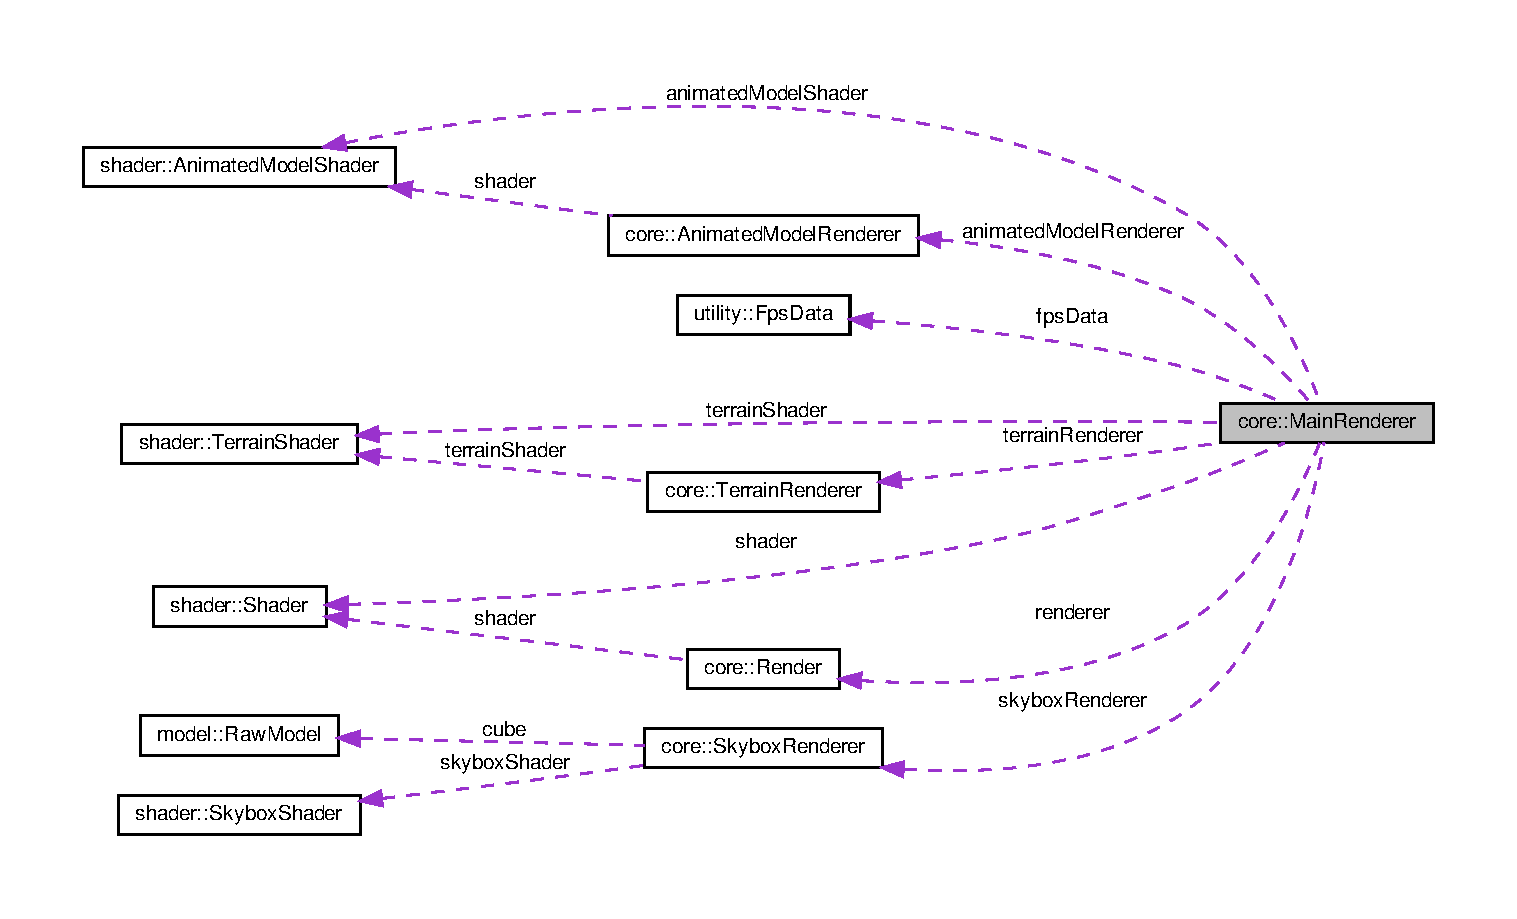
\includegraphics[width=350pt]{classcore_1_1MainRenderer__coll__graph}
\end{center}
\end{figure}
\subsection*{Javni članovi}
\begin{DoxyCompactItemize}
\item 
\hyperlink{classcore_1_1MainRenderer_ab005c6e84882d475f9579f9c09b2329d}{Main\+Renderer} ()
\begin{DoxyCompactList}\small\item\em Konstruktor klase. \end{DoxyCompactList}\item 
\hyperlink{classcore_1_1MainRenderer_a1e5f39d2178a7c5738efa9be9bd486da}{$\sim$\+Main\+Renderer} ()
\begin{DoxyCompactList}\small\item\em Destruktor klase. \end{DoxyCompactList}\item 
void \hyperlink{classcore_1_1MainRenderer_a3a8f4927df78f7b0ea7c4e5902569b1e}{render} (\hyperlink{classentity_1_1Light}{Light} $\ast$\hyperlink{namespacecore_a2324d96000e7c6d42570a0577e8f070b}{light}, \hyperlink{classentity_1_1Camera}{Camera} $\ast$\hyperlink{namespacecore_a9d645c490b142886301256f6cf9c65c2}{camera})
\begin{DoxyCompactList}\small\item\em Funkcija iscrtava teren i ostale entitete igre. \end{DoxyCompactList}\item 
void \hyperlink{classcore_1_1MainRenderer_ae5ffaef40e727ab758d7b2d36ed4e92a}{process\+Entity} (\hyperlink{classentity_1_1Entity}{Entity} $\ast$\hyperlink{namespacecore_aa710c0ea388433d2d80d1d1c67582eda}{entity})
\begin{DoxyCompactList}\small\item\em Funkcija obradjuje entitete i ubacuje ih u mapu entiteta. \end{DoxyCompactList}\item 
void \hyperlink{classcore_1_1MainRenderer_a4e8a3e6729a7d948761d6e74c48a6236}{process\+Terrain} (\hyperlink{classterrain_1_1Terrain}{Terrain} $\ast$\hyperlink{namespacecore_ac45da6f80dac9bead5c9310c27897f15}{terrain})
\begin{DoxyCompactList}\small\item\em Funkcija obradjuje terene i ubacuje ih u listu terena. \end{DoxyCompactList}\item 
void \hyperlink{classcore_1_1MainRenderer_af55caf59bc4f10718a18ecb3e784b778}{clean\+Up} (void)
\begin{DoxyCompactList}\small\item\em Funkcija poziva funkcije clean\+Up za sejdere entiteta i terena. \end{DoxyCompactList}\item 
void \hyperlink{classcore_1_1MainRenderer_a8e8be03c3b1f51ce0721cf52aa8f0f3c}{prepare} (void)
\begin{DoxyCompactList}\small\item\em Funkcija vrsi pripreme za iscrtavanje sadrzaja na ekran. \end{DoxyCompactList}\item 
void \hyperlink{classcore_1_1MainRenderer_abf659aace3015f29db1c3ea9561fff2f}{enable\+Culling} ()
\begin{DoxyCompactList}\small\item\em Funkcija onemogucava iscrtavanje zadnje strane objekata. \end{DoxyCompactList}\item 
void \hyperlink{classcore_1_1MainRenderer_a00a3d49faabb02f0984f521208681ac4}{disable\+Culling} ()
\begin{DoxyCompactList}\small\item\em Funkcija omogucava iscrtavanje zadnje strane objekata. \end{DoxyCompactList}\end{DoxyCompactItemize}
\subsection*{Privatni članovi}
\begin{DoxyCompactItemize}
\item 
\hyperlink{classshader_1_1Shader}{Shader} $\ast$ \hyperlink{classcore_1_1MainRenderer_a9e5b8ba9a151d64b79612b8631fc1255}{shader}
\begin{DoxyCompactList}\small\item\em Pokazivac na instancu klase Shader. \end{DoxyCompactList}\item 
\hyperlink{classcore_1_1Render}{Render} $\ast$ \hyperlink{classcore_1_1MainRenderer_a3cdbf7f833cac2e18e8bb7d3cdd7728d}{renderer}
\begin{DoxyCompactList}\small\item\em Pokazivac na instancu klase \hyperlink{classcore_1_1Render}{Render}. \end{DoxyCompactList}\item 
\hyperlink{classcore_1_1TerrainRenderer}{Terrain\+Renderer} $\ast$ \hyperlink{classcore_1_1MainRenderer_aba23d91ed6ade9c35600156c0e1f0d83}{terrain\+Renderer}
\begin{DoxyCompactList}\small\item\em Pokazivac na instancu klase \hyperlink{classcore_1_1TerrainRenderer}{Terrain\+Renderer}. \end{DoxyCompactList}\item 
\hyperlink{classshader_1_1TerrainShader}{Terrain\+Shader} $\ast$ \hyperlink{classcore_1_1MainRenderer_a502a7c6f714266f27601913496c396f3}{terrain\+Shader}
\begin{DoxyCompactList}\small\item\em Pokazivac na instancu klase Terrain\+Shader. \end{DoxyCompactList}\item 
map$<$ \hyperlink{classmodel_1_1TexturedModel}{Textured\+Model} $\ast$, list$<$ \hyperlink{classentity_1_1Entity}{Entity} $\ast$ $>$ $>$ \hyperlink{classcore_1_1MainRenderer_a609ec87995b16fcca439ce5585993fc4}{entities}
\begin{DoxyCompactList}\small\item\em Hes mapa koja sadrzi teksturisane modele i liste entiteta. \end{DoxyCompactList}\item 
list$<$ \hyperlink{classterrain_1_1Terrain}{Terrain} $\ast$ $>$ \hyperlink{classcore_1_1MainRenderer_ada8a51626222137e00ae29445e28f892}{terrains}
\begin{DoxyCompactList}\small\item\em Lista terena. \end{DoxyCompactList}\end{DoxyCompactItemize}


\subsection{Opširniji opis}
Klasa \hyperlink{classcore_1_1MainRenderer}{Main\+Renderer} je zaduzena za iscrtavanje sadrzaja na ekran. Tokom pokretanja prvo se vrsi priprema za iscrtavanje, a zatim se iscrtavaju teren igrac i ostali entiteti. 

\subsection{Dokumentacija konstruktora i destruktora}
\mbox{\Hypertarget{classcore_1_1MainRenderer_ab005c6e84882d475f9579f9c09b2329d}\label{classcore_1_1MainRenderer_ab005c6e84882d475f9579f9c09b2329d}} 
\index{core\+::\+Main\+Renderer@{core\+::\+Main\+Renderer}!Main\+Renderer@{Main\+Renderer}}
\index{Main\+Renderer@{Main\+Renderer}!core\+::\+Main\+Renderer@{core\+::\+Main\+Renderer}}
\subsubsection{\texorpdfstring{Main\+Renderer()}{MainRenderer()}}
{\footnotesize\ttfamily core\+::\+Main\+Renderer\+::\+Main\+Renderer (\begin{DoxyParamCaption}{ }\end{DoxyParamCaption})}



Konstruktor klase. 


\begin{DoxyParams}{Parametri}
{\em void} & \\
\hline
\end{DoxyParams}
\mbox{\Hypertarget{classcore_1_1MainRenderer_a1e5f39d2178a7c5738efa9be9bd486da}\label{classcore_1_1MainRenderer_a1e5f39d2178a7c5738efa9be9bd486da}} 
\index{core\+::\+Main\+Renderer@{core\+::\+Main\+Renderer}!````~Main\+Renderer@{$\sim$\+Main\+Renderer}}
\index{````~Main\+Renderer@{$\sim$\+Main\+Renderer}!core\+::\+Main\+Renderer@{core\+::\+Main\+Renderer}}
\subsubsection{\texorpdfstring{$\sim$\+Main\+Renderer()}{~MainRenderer()}}
{\footnotesize\ttfamily core\+::\+Main\+Renderer\+::$\sim$\+Main\+Renderer (\begin{DoxyParamCaption}{ }\end{DoxyParamCaption})}



Destruktor klase. 


\begin{DoxyParams}{Parametri}
{\em void} & \\
\hline
\end{DoxyParams}


\subsection{Dokumentacija funkcija članica}
\mbox{\Hypertarget{classcore_1_1MainRenderer_af55caf59bc4f10718a18ecb3e784b778}\label{classcore_1_1MainRenderer_af55caf59bc4f10718a18ecb3e784b778}} 
\index{core\+::\+Main\+Renderer@{core\+::\+Main\+Renderer}!clean\+Up@{clean\+Up}}
\index{clean\+Up@{clean\+Up}!core\+::\+Main\+Renderer@{core\+::\+Main\+Renderer}}
\subsubsection{\texorpdfstring{clean\+Up()}{cleanUp()}}
{\footnotesize\ttfamily void core\+::\+Main\+Renderer\+::clean\+Up (\begin{DoxyParamCaption}\item[{void}]{ }\end{DoxyParamCaption})}



Funkcija poziva funkcije clean\+Up za sejdere entiteta i terena. 


\begin{DoxyParams}{Parametri}
{\em void} & \\
\hline
\end{DoxyParams}
\begin{DoxyReturn}{Vrednost funkcije}
void 
\end{DoxyReturn}
\mbox{\Hypertarget{classcore_1_1MainRenderer_a00a3d49faabb02f0984f521208681ac4}\label{classcore_1_1MainRenderer_a00a3d49faabb02f0984f521208681ac4}} 
\index{core\+::\+Main\+Renderer@{core\+::\+Main\+Renderer}!disable\+Culling@{disable\+Culling}}
\index{disable\+Culling@{disable\+Culling}!core\+::\+Main\+Renderer@{core\+::\+Main\+Renderer}}
\subsubsection{\texorpdfstring{disable\+Culling()}{disableCulling()}}
{\footnotesize\ttfamily void core\+::\+Main\+Renderer\+::disable\+Culling (\begin{DoxyParamCaption}{ }\end{DoxyParamCaption})}



Funkcija omogucava iscrtavanje zadnje strane objekata. 


\begin{DoxyParams}{Parametri}
{\em void} & \\
\hline
\end{DoxyParams}
\begin{DoxyReturn}{Vrednost funkcije}
void 
\end{DoxyReturn}
\mbox{\Hypertarget{classcore_1_1MainRenderer_abf659aace3015f29db1c3ea9561fff2f}\label{classcore_1_1MainRenderer_abf659aace3015f29db1c3ea9561fff2f}} 
\index{core\+::\+Main\+Renderer@{core\+::\+Main\+Renderer}!enable\+Culling@{enable\+Culling}}
\index{enable\+Culling@{enable\+Culling}!core\+::\+Main\+Renderer@{core\+::\+Main\+Renderer}}
\subsubsection{\texorpdfstring{enable\+Culling()}{enableCulling()}}
{\footnotesize\ttfamily void core\+::\+Main\+Renderer\+::enable\+Culling (\begin{DoxyParamCaption}{ }\end{DoxyParamCaption})}



Funkcija onemogucava iscrtavanje zadnje strane objekata. 


\begin{DoxyParams}{Parametri}
{\em void} & \\
\hline
\end{DoxyParams}
\begin{DoxyReturn}{Vrednost funkcije}
void 
\end{DoxyReturn}
\mbox{\Hypertarget{classcore_1_1MainRenderer_a8e8be03c3b1f51ce0721cf52aa8f0f3c}\label{classcore_1_1MainRenderer_a8e8be03c3b1f51ce0721cf52aa8f0f3c}} 
\index{core\+::\+Main\+Renderer@{core\+::\+Main\+Renderer}!prepare@{prepare}}
\index{prepare@{prepare}!core\+::\+Main\+Renderer@{core\+::\+Main\+Renderer}}
\subsubsection{\texorpdfstring{prepare()}{prepare()}}
{\footnotesize\ttfamily void core\+::\+Main\+Renderer\+::prepare (\begin{DoxyParamCaption}\item[{void}]{ }\end{DoxyParamCaption})}



Funkcija vrsi pripreme za iscrtavanje sadrzaja na ekran. 


\begin{DoxyParams}{Parametri}
{\em void} & \\
\hline
\end{DoxyParams}
\begin{DoxyReturn}{Vrednost funkcije}
void 
\end{DoxyReturn}
\mbox{\Hypertarget{classcore_1_1MainRenderer_ae5ffaef40e727ab758d7b2d36ed4e92a}\label{classcore_1_1MainRenderer_ae5ffaef40e727ab758d7b2d36ed4e92a}} 
\index{core\+::\+Main\+Renderer@{core\+::\+Main\+Renderer}!process\+Entity@{process\+Entity}}
\index{process\+Entity@{process\+Entity}!core\+::\+Main\+Renderer@{core\+::\+Main\+Renderer}}
\subsubsection{\texorpdfstring{process\+Entity()}{processEntity()}}
{\footnotesize\ttfamily void core\+::\+Main\+Renderer\+::process\+Entity (\begin{DoxyParamCaption}\item[{\hyperlink{classentity_1_1Entity}{Entity} $\ast$}]{entity }\end{DoxyParamCaption})}



Funkcija obradjuje entitete i ubacuje ih u mapu entiteta. 


\begin{DoxyParams}{Parametri}
{\em entity} & Pokazivac na instancu klase Entity \\
\hline
\end{DoxyParams}
\begin{DoxyReturn}{Vrednost funkcije}
void 
\end{DoxyReturn}
\mbox{\Hypertarget{classcore_1_1MainRenderer_a4e8a3e6729a7d948761d6e74c48a6236}\label{classcore_1_1MainRenderer_a4e8a3e6729a7d948761d6e74c48a6236}} 
\index{core\+::\+Main\+Renderer@{core\+::\+Main\+Renderer}!process\+Terrain@{process\+Terrain}}
\index{process\+Terrain@{process\+Terrain}!core\+::\+Main\+Renderer@{core\+::\+Main\+Renderer}}
\subsubsection{\texorpdfstring{process\+Terrain()}{processTerrain()}}
{\footnotesize\ttfamily void core\+::\+Main\+Renderer\+::process\+Terrain (\begin{DoxyParamCaption}\item[{\hyperlink{classterrain_1_1Terrain}{Terrain} $\ast$}]{terrain }\end{DoxyParamCaption})}



Funkcija obradjuje terene i ubacuje ih u listu terena. 


\begin{DoxyParams}{Parametri}
{\em terrain} & Pokazivac na instancu klase Terrain \\
\hline
\end{DoxyParams}
\begin{DoxyReturn}{Vrednost funkcije}
void 
\end{DoxyReturn}
\mbox{\Hypertarget{classcore_1_1MainRenderer_a3a8f4927df78f7b0ea7c4e5902569b1e}\label{classcore_1_1MainRenderer_a3a8f4927df78f7b0ea7c4e5902569b1e}} 
\index{core\+::\+Main\+Renderer@{core\+::\+Main\+Renderer}!render@{render}}
\index{render@{render}!core\+::\+Main\+Renderer@{core\+::\+Main\+Renderer}}
\subsubsection{\texorpdfstring{render()}{render()}}
{\footnotesize\ttfamily void core\+::\+Main\+Renderer\+::render (\begin{DoxyParamCaption}\item[{\hyperlink{classentity_1_1Light}{Light} $\ast$}]{light,  }\item[{\hyperlink{classentity_1_1Camera}{Camera} $\ast$}]{camera }\end{DoxyParamCaption})}



Funkcija iscrtava teren i ostale entitete igre. 


\begin{DoxyParams}{Parametri}
{\em light} & Pokazivac na instancu klase Light \\
\hline
{\em camera} & Pokazivac na instancu klase Camera \\
\hline
\end{DoxyParams}
\begin{DoxyReturn}{Vrednost funkcije}
void 
\end{DoxyReturn}


\subsection{Dokumentacija atributa}
\mbox{\Hypertarget{classcore_1_1MainRenderer_a609ec87995b16fcca439ce5585993fc4}\label{classcore_1_1MainRenderer_a609ec87995b16fcca439ce5585993fc4}} 
\index{core\+::\+Main\+Renderer@{core\+::\+Main\+Renderer}!entities@{entities}}
\index{entities@{entities}!core\+::\+Main\+Renderer@{core\+::\+Main\+Renderer}}
\subsubsection{\texorpdfstring{entities}{entities}}
{\footnotesize\ttfamily map$<$\hyperlink{classmodel_1_1TexturedModel}{Textured\+Model} $\ast$, list$<$\hyperlink{classentity_1_1Entity}{Entity} $\ast$$>$ $>$ core\+::\+Main\+Renderer\+::entities\hspace{0.3cm}{\ttfamily [private]}}



Hes mapa koja sadrzi teksturisane modele i liste entiteta. 

\mbox{\Hypertarget{classcore_1_1MainRenderer_a3cdbf7f833cac2e18e8bb7d3cdd7728d}\label{classcore_1_1MainRenderer_a3cdbf7f833cac2e18e8bb7d3cdd7728d}} 
\index{core\+::\+Main\+Renderer@{core\+::\+Main\+Renderer}!renderer@{renderer}}
\index{renderer@{renderer}!core\+::\+Main\+Renderer@{core\+::\+Main\+Renderer}}
\subsubsection{\texorpdfstring{renderer}{renderer}}
{\footnotesize\ttfamily \hyperlink{classcore_1_1Render}{Render}$\ast$ core\+::\+Main\+Renderer\+::renderer\hspace{0.3cm}{\ttfamily [private]}}



Pokazivac na instancu klase \hyperlink{classcore_1_1Render}{Render}. 

\mbox{\Hypertarget{classcore_1_1MainRenderer_a9e5b8ba9a151d64b79612b8631fc1255}\label{classcore_1_1MainRenderer_a9e5b8ba9a151d64b79612b8631fc1255}} 
\index{core\+::\+Main\+Renderer@{core\+::\+Main\+Renderer}!shader@{shader}}
\index{shader@{shader}!core\+::\+Main\+Renderer@{core\+::\+Main\+Renderer}}
\subsubsection{\texorpdfstring{shader}{shader}}
{\footnotesize\ttfamily \hyperlink{classshader_1_1Shader}{Shader}$\ast$ core\+::\+Main\+Renderer\+::shader\hspace{0.3cm}{\ttfamily [private]}}



Pokazivac na instancu klase Shader. 

\mbox{\Hypertarget{classcore_1_1MainRenderer_aba23d91ed6ade9c35600156c0e1f0d83}\label{classcore_1_1MainRenderer_aba23d91ed6ade9c35600156c0e1f0d83}} 
\index{core\+::\+Main\+Renderer@{core\+::\+Main\+Renderer}!terrain\+Renderer@{terrain\+Renderer}}
\index{terrain\+Renderer@{terrain\+Renderer}!core\+::\+Main\+Renderer@{core\+::\+Main\+Renderer}}
\subsubsection{\texorpdfstring{terrain\+Renderer}{terrainRenderer}}
{\footnotesize\ttfamily \hyperlink{classcore_1_1TerrainRenderer}{Terrain\+Renderer}$\ast$ core\+::\+Main\+Renderer\+::terrain\+Renderer\hspace{0.3cm}{\ttfamily [private]}}



Pokazivac na instancu klase \hyperlink{classcore_1_1TerrainRenderer}{Terrain\+Renderer}. 

\mbox{\Hypertarget{classcore_1_1MainRenderer_ada8a51626222137e00ae29445e28f892}\label{classcore_1_1MainRenderer_ada8a51626222137e00ae29445e28f892}} 
\index{core\+::\+Main\+Renderer@{core\+::\+Main\+Renderer}!terrains@{terrains}}
\index{terrains@{terrains}!core\+::\+Main\+Renderer@{core\+::\+Main\+Renderer}}
\subsubsection{\texorpdfstring{terrains}{terrains}}
{\footnotesize\ttfamily list$<$\hyperlink{classterrain_1_1Terrain}{Terrain} $\ast$$>$ core\+::\+Main\+Renderer\+::terrains\hspace{0.3cm}{\ttfamily [private]}}



Lista terena. 

\mbox{\Hypertarget{classcore_1_1MainRenderer_a502a7c6f714266f27601913496c396f3}\label{classcore_1_1MainRenderer_a502a7c6f714266f27601913496c396f3}} 
\index{core\+::\+Main\+Renderer@{core\+::\+Main\+Renderer}!terrain\+Shader@{terrain\+Shader}}
\index{terrain\+Shader@{terrain\+Shader}!core\+::\+Main\+Renderer@{core\+::\+Main\+Renderer}}
\subsubsection{\texorpdfstring{terrain\+Shader}{terrainShader}}
{\footnotesize\ttfamily \hyperlink{classshader_1_1TerrainShader}{Terrain\+Shader}$\ast$ core\+::\+Main\+Renderer\+::terrain\+Shader\hspace{0.3cm}{\ttfamily [private]}}



Pokazivac na instancu klase Terrain\+Shader. 



Dokumentacija ove klase je napravljena na osnovu sledećih datoteka\+:\begin{DoxyCompactItemize}
\item 
/home/dusan/\+Documents/\+Projects/\+R\+G102-\/vitez-\/reda-\/zmaja/include/core/\hyperlink{MainRenderer_8h}{Main\+Renderer.\+h}\item 
/home/dusan/\+Documents/\+Projects/\+R\+G102-\/vitez-\/reda-\/zmaja/src/core/\hyperlink{MainRenderer_8cpp}{Main\+Renderer.\+cpp}\end{DoxyCompactItemize}

\hypertarget{structtinyobj_1_1material__t}{}\section{Dokumentacija strukture tinyobj\+:\+:material\+\_\+t}
\label{structtinyobj_1_1material__t}\index{tinyobj\+::material\+\_\+t@{tinyobj\+::material\+\_\+t}}


{\ttfamily \#include $<$tiny\+\_\+obj\+\_\+loader.\+h$>$}



Klasni dijagram za tinyobj\+:\+:material\+\_\+t\+:\nopagebreak
\begin{figure}[H]
\begin{center}
\leavevmode
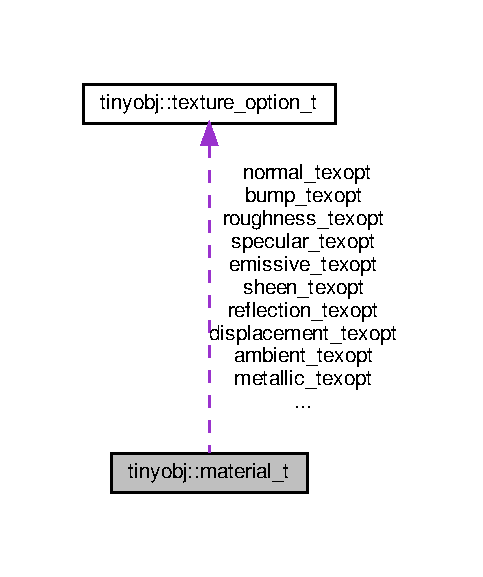
\includegraphics[width=232pt]{structtinyobj_1_1material__t__coll__graph}
\end{center}
\end{figure}
\subsection*{Javni članovi}
\begin{DoxyCompactItemize}
\item 
std\+::string \hyperlink{structtinyobj_1_1material__t_a41fde82dd0ec383b1d4ee258c4e4a1b9}{name}
\item 
\hyperlink{namespacetinyobj_ad5ca7469ff56bf0d8423120cfd99adce}{real\+\_\+t} \hyperlink{structtinyobj_1_1material__t_ac69088b2904edf45631e3e56329f4549}{ambient} \mbox{[}3\mbox{]}
\item 
\hyperlink{namespacetinyobj_ad5ca7469ff56bf0d8423120cfd99adce}{real\+\_\+t} \hyperlink{structtinyobj_1_1material__t_a783cdfe69d52d4011bdcad54869ac453}{diffuse} \mbox{[}3\mbox{]}
\item 
\hyperlink{namespacetinyobj_ad5ca7469ff56bf0d8423120cfd99adce}{real\+\_\+t} \hyperlink{structtinyobj_1_1material__t_ac03664c37a93e4da3441036abd0ad153}{specular} \mbox{[}3\mbox{]}
\item 
\hyperlink{namespacetinyobj_ad5ca7469ff56bf0d8423120cfd99adce}{real\+\_\+t} \hyperlink{structtinyobj_1_1material__t_ab6d488962642d79b409bb831d9f2b1f3}{transmittance} \mbox{[}3\mbox{]}
\item 
\hyperlink{namespacetinyobj_ad5ca7469ff56bf0d8423120cfd99adce}{real\+\_\+t} \hyperlink{structtinyobj_1_1material__t_a6ceb4407ddc81f6750eee96d12d784e8}{emission} \mbox{[}3\mbox{]}
\item 
\hyperlink{namespacetinyobj_ad5ca7469ff56bf0d8423120cfd99adce}{real\+\_\+t} \hyperlink{structtinyobj_1_1material__t_aed153afc668c6b4760da57e0e63e0e97}{shininess}
\item 
\hyperlink{namespacetinyobj_ad5ca7469ff56bf0d8423120cfd99adce}{real\+\_\+t} \hyperlink{structtinyobj_1_1material__t_ac5d5fed58b485804119ed374ea90709e}{ior}
\item 
\hyperlink{namespacetinyobj_ad5ca7469ff56bf0d8423120cfd99adce}{real\+\_\+t} \hyperlink{structtinyobj_1_1material__t_a61e3561bf67f6faec6ac4f551f9956cb}{dissolve}
\item 
int \hyperlink{structtinyobj_1_1material__t_af846245315bd70c1a4f815dfdd6b80cc}{illum}
\item 
int \hyperlink{structtinyobj_1_1material__t_a6b1814d1066609178c81d2a4f7b34bd8}{dummy}
\item 
std\+::string \hyperlink{structtinyobj_1_1material__t_ae988eed637f368374becbb672798a45e}{ambient\+\_\+texname}
\item 
std\+::string \hyperlink{structtinyobj_1_1material__t_ad7f71a301a261fca07d2e50edccc792d}{diffuse\+\_\+texname}
\item 
std\+::string \hyperlink{structtinyobj_1_1material__t_aed8c38d64472ba0db5186dba800b1b34}{specular\+\_\+texname}
\item 
std\+::string \hyperlink{structtinyobj_1_1material__t_a5c0e981297646f1fc1aeba616692c41b}{specular\+\_\+highlight\+\_\+texname}
\item 
std\+::string \hyperlink{structtinyobj_1_1material__t_aceb73086232f1cdd82f956fe8c6efcfb}{bump\+\_\+texname}
\item 
std\+::string \hyperlink{structtinyobj_1_1material__t_ab69842db3e67cc7d4dcd8bfe02590f92}{displacement\+\_\+texname}
\item 
std\+::string \hyperlink{structtinyobj_1_1material__t_a1b0225fd76de506f089fdedbf2c66dec}{alpha\+\_\+texname}
\item 
std\+::string \hyperlink{structtinyobj_1_1material__t_a111faaae52874d8715c7719acf60d726}{reflection\+\_\+texname}
\item 
\hyperlink{structtinyobj_1_1texture__option__t}{texture\+\_\+option\+\_\+t} \hyperlink{structtinyobj_1_1material__t_ad168f86b0f3f67666b102f9a26a2170b}{ambient\+\_\+texopt}
\item 
\hyperlink{structtinyobj_1_1texture__option__t}{texture\+\_\+option\+\_\+t} \hyperlink{structtinyobj_1_1material__t_a170412a1e339856e55d5cec406ecc196}{diffuse\+\_\+texopt}
\item 
\hyperlink{structtinyobj_1_1texture__option__t}{texture\+\_\+option\+\_\+t} \hyperlink{structtinyobj_1_1material__t_aec86b92157df1e714aeb1f28ebabae24}{specular\+\_\+texopt}
\item 
\hyperlink{structtinyobj_1_1texture__option__t}{texture\+\_\+option\+\_\+t} \hyperlink{structtinyobj_1_1material__t_a9bfc943306506fa35abbb4377b8c071e}{specular\+\_\+highlight\+\_\+texopt}
\item 
\hyperlink{structtinyobj_1_1texture__option__t}{texture\+\_\+option\+\_\+t} \hyperlink{structtinyobj_1_1material__t_a77cb124464a606ad2b649196e72c39a0}{bump\+\_\+texopt}
\item 
\hyperlink{structtinyobj_1_1texture__option__t}{texture\+\_\+option\+\_\+t} \hyperlink{structtinyobj_1_1material__t_a6f28d7a04ebb6435c62adb502847f4c3}{displacement\+\_\+texopt}
\item 
\hyperlink{structtinyobj_1_1texture__option__t}{texture\+\_\+option\+\_\+t} \hyperlink{structtinyobj_1_1material__t_adb6fdf38b462c4bd91fc2927282a3fc1}{alpha\+\_\+texopt}
\item 
\hyperlink{structtinyobj_1_1texture__option__t}{texture\+\_\+option\+\_\+t} \hyperlink{structtinyobj_1_1material__t_a8e9e796988061cf2446f65d79a6f6ae9}{reflection\+\_\+texopt}
\item 
\hyperlink{namespacetinyobj_ad5ca7469ff56bf0d8423120cfd99adce}{real\+\_\+t} \hyperlink{structtinyobj_1_1material__t_a7e26f199e4a308bd9fd224349e266cea}{roughness}
\item 
\hyperlink{namespacetinyobj_ad5ca7469ff56bf0d8423120cfd99adce}{real\+\_\+t} \hyperlink{structtinyobj_1_1material__t_a0d5be8695d84eda23ac048e09d611fad}{metallic}
\item 
\hyperlink{namespacetinyobj_ad5ca7469ff56bf0d8423120cfd99adce}{real\+\_\+t} \hyperlink{structtinyobj_1_1material__t_a9c56ee4bf20385c8968a8b97b5d115c1}{sheen}
\item 
\hyperlink{namespacetinyobj_ad5ca7469ff56bf0d8423120cfd99adce}{real\+\_\+t} \hyperlink{structtinyobj_1_1material__t_a324dd4bb8475271e31aeb0a5959af745}{clearcoat\+\_\+thickness}
\item 
\hyperlink{namespacetinyobj_ad5ca7469ff56bf0d8423120cfd99adce}{real\+\_\+t} \hyperlink{structtinyobj_1_1material__t_a0856eb3210823262539af42aa2f5a63e}{clearcoat\+\_\+roughness}
\item 
\hyperlink{namespacetinyobj_ad5ca7469ff56bf0d8423120cfd99adce}{real\+\_\+t} \hyperlink{structtinyobj_1_1material__t_a0bd6ee79907285b19365849ba50965b1}{anisotropy}
\item 
\hyperlink{namespacetinyobj_ad5ca7469ff56bf0d8423120cfd99adce}{real\+\_\+t} \hyperlink{structtinyobj_1_1material__t_ab1b9216b525cc02d2f6392db71ce0f59}{anisotropy\+\_\+rotation}
\item 
\hyperlink{namespacetinyobj_ad5ca7469ff56bf0d8423120cfd99adce}{real\+\_\+t} \hyperlink{structtinyobj_1_1material__t_af16b7962e5809504ec31ebf9631422b7}{pad0}
\item 
std\+::string \hyperlink{structtinyobj_1_1material__t_a7d7a7791ad94f2a5eadc2c8ee8c9a902}{roughness\+\_\+texname}
\item 
std\+::string \hyperlink{structtinyobj_1_1material__t_acf05b62ec21680f4d803f02a59ad183a}{metallic\+\_\+texname}
\item 
std\+::string \hyperlink{structtinyobj_1_1material__t_a0410f86a8fbe3f5d533d440f07781c04}{sheen\+\_\+texname}
\item 
std\+::string \hyperlink{structtinyobj_1_1material__t_a63bb93815630b2dfca986ae17c51b919}{emissive\+\_\+texname}
\item 
std\+::string \hyperlink{structtinyobj_1_1material__t_a7512ccf46044357bea1739d583871578}{normal\+\_\+texname}
\item 
\hyperlink{structtinyobj_1_1texture__option__t}{texture\+\_\+option\+\_\+t} \hyperlink{structtinyobj_1_1material__t_aa02a56f4de95ab212e19a5d77b1f2d91}{roughness\+\_\+texopt}
\item 
\hyperlink{structtinyobj_1_1texture__option__t}{texture\+\_\+option\+\_\+t} \hyperlink{structtinyobj_1_1material__t_abbae6c6e634f9899c3974731c554be21}{metallic\+\_\+texopt}
\item 
\hyperlink{structtinyobj_1_1texture__option__t}{texture\+\_\+option\+\_\+t} \hyperlink{structtinyobj_1_1material__t_a60a907d53aed60591b8d78ae220c7c4a}{sheen\+\_\+texopt}
\item 
\hyperlink{structtinyobj_1_1texture__option__t}{texture\+\_\+option\+\_\+t} \hyperlink{structtinyobj_1_1material__t_a7a2da381cdabd6655aaed320d5b1ffe3}{emissive\+\_\+texopt}
\item 
\hyperlink{structtinyobj_1_1texture__option__t}{texture\+\_\+option\+\_\+t} \hyperlink{structtinyobj_1_1material__t_aa0087d1bfcaf0a195f8c244970c2ef4e}{normal\+\_\+texopt}
\item 
int \hyperlink{structtinyobj_1_1material__t_a84cd388a80784aaaac4a03267d77f994}{pad2}
\item 
std\+::map$<$ std\+::string, std\+::string $>$ \hyperlink{structtinyobj_1_1material__t_a18b700227c94d410ed1aa550c7fa9226}{unknown\+\_\+parameter}
\end{DoxyCompactItemize}


\subsection{Dokumentacija atributa}
\mbox{\Hypertarget{structtinyobj_1_1material__t_a1b0225fd76de506f089fdedbf2c66dec}\label{structtinyobj_1_1material__t_a1b0225fd76de506f089fdedbf2c66dec}} 
\index{tinyobj\+::material\+\_\+t@{tinyobj\+::material\+\_\+t}!alpha\+\_\+texname@{alpha\+\_\+texname}}
\index{alpha\+\_\+texname@{alpha\+\_\+texname}!tinyobj\+::material\+\_\+t@{tinyobj\+::material\+\_\+t}}
\subsubsection{\texorpdfstring{alpha\+\_\+texname}{alpha\_texname}}
{\footnotesize\ttfamily std\+::string tinyobj\+::material\+\_\+t\+::alpha\+\_\+texname}

\mbox{\Hypertarget{structtinyobj_1_1material__t_adb6fdf38b462c4bd91fc2927282a3fc1}\label{structtinyobj_1_1material__t_adb6fdf38b462c4bd91fc2927282a3fc1}} 
\index{tinyobj\+::material\+\_\+t@{tinyobj\+::material\+\_\+t}!alpha\+\_\+texopt@{alpha\+\_\+texopt}}
\index{alpha\+\_\+texopt@{alpha\+\_\+texopt}!tinyobj\+::material\+\_\+t@{tinyobj\+::material\+\_\+t}}
\subsubsection{\texorpdfstring{alpha\+\_\+texopt}{alpha\_texopt}}
{\footnotesize\ttfamily \hyperlink{structtinyobj_1_1texture__option__t}{texture\+\_\+option\+\_\+t} tinyobj\+::material\+\_\+t\+::alpha\+\_\+texopt}

\mbox{\Hypertarget{structtinyobj_1_1material__t_ac69088b2904edf45631e3e56329f4549}\label{structtinyobj_1_1material__t_ac69088b2904edf45631e3e56329f4549}} 
\index{tinyobj\+::material\+\_\+t@{tinyobj\+::material\+\_\+t}!ambient@{ambient}}
\index{ambient@{ambient}!tinyobj\+::material\+\_\+t@{tinyobj\+::material\+\_\+t}}
\subsubsection{\texorpdfstring{ambient}{ambient}}
{\footnotesize\ttfamily \hyperlink{namespacetinyobj_ad5ca7469ff56bf0d8423120cfd99adce}{real\+\_\+t} tinyobj\+::material\+\_\+t\+::ambient\mbox{[}3\mbox{]}}

\mbox{\Hypertarget{structtinyobj_1_1material__t_ae988eed637f368374becbb672798a45e}\label{structtinyobj_1_1material__t_ae988eed637f368374becbb672798a45e}} 
\index{tinyobj\+::material\+\_\+t@{tinyobj\+::material\+\_\+t}!ambient\+\_\+texname@{ambient\+\_\+texname}}
\index{ambient\+\_\+texname@{ambient\+\_\+texname}!tinyobj\+::material\+\_\+t@{tinyobj\+::material\+\_\+t}}
\subsubsection{\texorpdfstring{ambient\+\_\+texname}{ambient\_texname}}
{\footnotesize\ttfamily std\+::string tinyobj\+::material\+\_\+t\+::ambient\+\_\+texname}

\mbox{\Hypertarget{structtinyobj_1_1material__t_ad168f86b0f3f67666b102f9a26a2170b}\label{structtinyobj_1_1material__t_ad168f86b0f3f67666b102f9a26a2170b}} 
\index{tinyobj\+::material\+\_\+t@{tinyobj\+::material\+\_\+t}!ambient\+\_\+texopt@{ambient\+\_\+texopt}}
\index{ambient\+\_\+texopt@{ambient\+\_\+texopt}!tinyobj\+::material\+\_\+t@{tinyobj\+::material\+\_\+t}}
\subsubsection{\texorpdfstring{ambient\+\_\+texopt}{ambient\_texopt}}
{\footnotesize\ttfamily \hyperlink{structtinyobj_1_1texture__option__t}{texture\+\_\+option\+\_\+t} tinyobj\+::material\+\_\+t\+::ambient\+\_\+texopt}

\mbox{\Hypertarget{structtinyobj_1_1material__t_a0bd6ee79907285b19365849ba50965b1}\label{structtinyobj_1_1material__t_a0bd6ee79907285b19365849ba50965b1}} 
\index{tinyobj\+::material\+\_\+t@{tinyobj\+::material\+\_\+t}!anisotropy@{anisotropy}}
\index{anisotropy@{anisotropy}!tinyobj\+::material\+\_\+t@{tinyobj\+::material\+\_\+t}}
\subsubsection{\texorpdfstring{anisotropy}{anisotropy}}
{\footnotesize\ttfamily \hyperlink{namespacetinyobj_ad5ca7469ff56bf0d8423120cfd99adce}{real\+\_\+t} tinyobj\+::material\+\_\+t\+::anisotropy}

\mbox{\Hypertarget{structtinyobj_1_1material__t_ab1b9216b525cc02d2f6392db71ce0f59}\label{structtinyobj_1_1material__t_ab1b9216b525cc02d2f6392db71ce0f59}} 
\index{tinyobj\+::material\+\_\+t@{tinyobj\+::material\+\_\+t}!anisotropy\+\_\+rotation@{anisotropy\+\_\+rotation}}
\index{anisotropy\+\_\+rotation@{anisotropy\+\_\+rotation}!tinyobj\+::material\+\_\+t@{tinyobj\+::material\+\_\+t}}
\subsubsection{\texorpdfstring{anisotropy\+\_\+rotation}{anisotropy\_rotation}}
{\footnotesize\ttfamily \hyperlink{namespacetinyobj_ad5ca7469ff56bf0d8423120cfd99adce}{real\+\_\+t} tinyobj\+::material\+\_\+t\+::anisotropy\+\_\+rotation}

\mbox{\Hypertarget{structtinyobj_1_1material__t_aceb73086232f1cdd82f956fe8c6efcfb}\label{structtinyobj_1_1material__t_aceb73086232f1cdd82f956fe8c6efcfb}} 
\index{tinyobj\+::material\+\_\+t@{tinyobj\+::material\+\_\+t}!bump\+\_\+texname@{bump\+\_\+texname}}
\index{bump\+\_\+texname@{bump\+\_\+texname}!tinyobj\+::material\+\_\+t@{tinyobj\+::material\+\_\+t}}
\subsubsection{\texorpdfstring{bump\+\_\+texname}{bump\_texname}}
{\footnotesize\ttfamily std\+::string tinyobj\+::material\+\_\+t\+::bump\+\_\+texname}

\mbox{\Hypertarget{structtinyobj_1_1material__t_a77cb124464a606ad2b649196e72c39a0}\label{structtinyobj_1_1material__t_a77cb124464a606ad2b649196e72c39a0}} 
\index{tinyobj\+::material\+\_\+t@{tinyobj\+::material\+\_\+t}!bump\+\_\+texopt@{bump\+\_\+texopt}}
\index{bump\+\_\+texopt@{bump\+\_\+texopt}!tinyobj\+::material\+\_\+t@{tinyobj\+::material\+\_\+t}}
\subsubsection{\texorpdfstring{bump\+\_\+texopt}{bump\_texopt}}
{\footnotesize\ttfamily \hyperlink{structtinyobj_1_1texture__option__t}{texture\+\_\+option\+\_\+t} tinyobj\+::material\+\_\+t\+::bump\+\_\+texopt}

\mbox{\Hypertarget{structtinyobj_1_1material__t_a0856eb3210823262539af42aa2f5a63e}\label{structtinyobj_1_1material__t_a0856eb3210823262539af42aa2f5a63e}} 
\index{tinyobj\+::material\+\_\+t@{tinyobj\+::material\+\_\+t}!clearcoat\+\_\+roughness@{clearcoat\+\_\+roughness}}
\index{clearcoat\+\_\+roughness@{clearcoat\+\_\+roughness}!tinyobj\+::material\+\_\+t@{tinyobj\+::material\+\_\+t}}
\subsubsection{\texorpdfstring{clearcoat\+\_\+roughness}{clearcoat\_roughness}}
{\footnotesize\ttfamily \hyperlink{namespacetinyobj_ad5ca7469ff56bf0d8423120cfd99adce}{real\+\_\+t} tinyobj\+::material\+\_\+t\+::clearcoat\+\_\+roughness}

\mbox{\Hypertarget{structtinyobj_1_1material__t_a324dd4bb8475271e31aeb0a5959af745}\label{structtinyobj_1_1material__t_a324dd4bb8475271e31aeb0a5959af745}} 
\index{tinyobj\+::material\+\_\+t@{tinyobj\+::material\+\_\+t}!clearcoat\+\_\+thickness@{clearcoat\+\_\+thickness}}
\index{clearcoat\+\_\+thickness@{clearcoat\+\_\+thickness}!tinyobj\+::material\+\_\+t@{tinyobj\+::material\+\_\+t}}
\subsubsection{\texorpdfstring{clearcoat\+\_\+thickness}{clearcoat\_thickness}}
{\footnotesize\ttfamily \hyperlink{namespacetinyobj_ad5ca7469ff56bf0d8423120cfd99adce}{real\+\_\+t} tinyobj\+::material\+\_\+t\+::clearcoat\+\_\+thickness}

\mbox{\Hypertarget{structtinyobj_1_1material__t_a783cdfe69d52d4011bdcad54869ac453}\label{structtinyobj_1_1material__t_a783cdfe69d52d4011bdcad54869ac453}} 
\index{tinyobj\+::material\+\_\+t@{tinyobj\+::material\+\_\+t}!diffuse@{diffuse}}
\index{diffuse@{diffuse}!tinyobj\+::material\+\_\+t@{tinyobj\+::material\+\_\+t}}
\subsubsection{\texorpdfstring{diffuse}{diffuse}}
{\footnotesize\ttfamily \hyperlink{namespacetinyobj_ad5ca7469ff56bf0d8423120cfd99adce}{real\+\_\+t} tinyobj\+::material\+\_\+t\+::diffuse\mbox{[}3\mbox{]}}

\mbox{\Hypertarget{structtinyobj_1_1material__t_ad7f71a301a261fca07d2e50edccc792d}\label{structtinyobj_1_1material__t_ad7f71a301a261fca07d2e50edccc792d}} 
\index{tinyobj\+::material\+\_\+t@{tinyobj\+::material\+\_\+t}!diffuse\+\_\+texname@{diffuse\+\_\+texname}}
\index{diffuse\+\_\+texname@{diffuse\+\_\+texname}!tinyobj\+::material\+\_\+t@{tinyobj\+::material\+\_\+t}}
\subsubsection{\texorpdfstring{diffuse\+\_\+texname}{diffuse\_texname}}
{\footnotesize\ttfamily std\+::string tinyobj\+::material\+\_\+t\+::diffuse\+\_\+texname}

\mbox{\Hypertarget{structtinyobj_1_1material__t_a170412a1e339856e55d5cec406ecc196}\label{structtinyobj_1_1material__t_a170412a1e339856e55d5cec406ecc196}} 
\index{tinyobj\+::material\+\_\+t@{tinyobj\+::material\+\_\+t}!diffuse\+\_\+texopt@{diffuse\+\_\+texopt}}
\index{diffuse\+\_\+texopt@{diffuse\+\_\+texopt}!tinyobj\+::material\+\_\+t@{tinyobj\+::material\+\_\+t}}
\subsubsection{\texorpdfstring{diffuse\+\_\+texopt}{diffuse\_texopt}}
{\footnotesize\ttfamily \hyperlink{structtinyobj_1_1texture__option__t}{texture\+\_\+option\+\_\+t} tinyobj\+::material\+\_\+t\+::diffuse\+\_\+texopt}

\mbox{\Hypertarget{structtinyobj_1_1material__t_ab69842db3e67cc7d4dcd8bfe02590f92}\label{structtinyobj_1_1material__t_ab69842db3e67cc7d4dcd8bfe02590f92}} 
\index{tinyobj\+::material\+\_\+t@{tinyobj\+::material\+\_\+t}!displacement\+\_\+texname@{displacement\+\_\+texname}}
\index{displacement\+\_\+texname@{displacement\+\_\+texname}!tinyobj\+::material\+\_\+t@{tinyobj\+::material\+\_\+t}}
\subsubsection{\texorpdfstring{displacement\+\_\+texname}{displacement\_texname}}
{\footnotesize\ttfamily std\+::string tinyobj\+::material\+\_\+t\+::displacement\+\_\+texname}

\mbox{\Hypertarget{structtinyobj_1_1material__t_a6f28d7a04ebb6435c62adb502847f4c3}\label{structtinyobj_1_1material__t_a6f28d7a04ebb6435c62adb502847f4c3}} 
\index{tinyobj\+::material\+\_\+t@{tinyobj\+::material\+\_\+t}!displacement\+\_\+texopt@{displacement\+\_\+texopt}}
\index{displacement\+\_\+texopt@{displacement\+\_\+texopt}!tinyobj\+::material\+\_\+t@{tinyobj\+::material\+\_\+t}}
\subsubsection{\texorpdfstring{displacement\+\_\+texopt}{displacement\_texopt}}
{\footnotesize\ttfamily \hyperlink{structtinyobj_1_1texture__option__t}{texture\+\_\+option\+\_\+t} tinyobj\+::material\+\_\+t\+::displacement\+\_\+texopt}

\mbox{\Hypertarget{structtinyobj_1_1material__t_a61e3561bf67f6faec6ac4f551f9956cb}\label{structtinyobj_1_1material__t_a61e3561bf67f6faec6ac4f551f9956cb}} 
\index{tinyobj\+::material\+\_\+t@{tinyobj\+::material\+\_\+t}!dissolve@{dissolve}}
\index{dissolve@{dissolve}!tinyobj\+::material\+\_\+t@{tinyobj\+::material\+\_\+t}}
\subsubsection{\texorpdfstring{dissolve}{dissolve}}
{\footnotesize\ttfamily \hyperlink{namespacetinyobj_ad5ca7469ff56bf0d8423120cfd99adce}{real\+\_\+t} tinyobj\+::material\+\_\+t\+::dissolve}

\mbox{\Hypertarget{structtinyobj_1_1material__t_a6b1814d1066609178c81d2a4f7b34bd8}\label{structtinyobj_1_1material__t_a6b1814d1066609178c81d2a4f7b34bd8}} 
\index{tinyobj\+::material\+\_\+t@{tinyobj\+::material\+\_\+t}!dummy@{dummy}}
\index{dummy@{dummy}!tinyobj\+::material\+\_\+t@{tinyobj\+::material\+\_\+t}}
\subsubsection{\texorpdfstring{dummy}{dummy}}
{\footnotesize\ttfamily int tinyobj\+::material\+\_\+t\+::dummy}

\mbox{\Hypertarget{structtinyobj_1_1material__t_a6ceb4407ddc81f6750eee96d12d784e8}\label{structtinyobj_1_1material__t_a6ceb4407ddc81f6750eee96d12d784e8}} 
\index{tinyobj\+::material\+\_\+t@{tinyobj\+::material\+\_\+t}!emission@{emission}}
\index{emission@{emission}!tinyobj\+::material\+\_\+t@{tinyobj\+::material\+\_\+t}}
\subsubsection{\texorpdfstring{emission}{emission}}
{\footnotesize\ttfamily \hyperlink{namespacetinyobj_ad5ca7469ff56bf0d8423120cfd99adce}{real\+\_\+t} tinyobj\+::material\+\_\+t\+::emission\mbox{[}3\mbox{]}}

\mbox{\Hypertarget{structtinyobj_1_1material__t_a63bb93815630b2dfca986ae17c51b919}\label{structtinyobj_1_1material__t_a63bb93815630b2dfca986ae17c51b919}} 
\index{tinyobj\+::material\+\_\+t@{tinyobj\+::material\+\_\+t}!emissive\+\_\+texname@{emissive\+\_\+texname}}
\index{emissive\+\_\+texname@{emissive\+\_\+texname}!tinyobj\+::material\+\_\+t@{tinyobj\+::material\+\_\+t}}
\subsubsection{\texorpdfstring{emissive\+\_\+texname}{emissive\_texname}}
{\footnotesize\ttfamily std\+::string tinyobj\+::material\+\_\+t\+::emissive\+\_\+texname}

\mbox{\Hypertarget{structtinyobj_1_1material__t_a7a2da381cdabd6655aaed320d5b1ffe3}\label{structtinyobj_1_1material__t_a7a2da381cdabd6655aaed320d5b1ffe3}} 
\index{tinyobj\+::material\+\_\+t@{tinyobj\+::material\+\_\+t}!emissive\+\_\+texopt@{emissive\+\_\+texopt}}
\index{emissive\+\_\+texopt@{emissive\+\_\+texopt}!tinyobj\+::material\+\_\+t@{tinyobj\+::material\+\_\+t}}
\subsubsection{\texorpdfstring{emissive\+\_\+texopt}{emissive\_texopt}}
{\footnotesize\ttfamily \hyperlink{structtinyobj_1_1texture__option__t}{texture\+\_\+option\+\_\+t} tinyobj\+::material\+\_\+t\+::emissive\+\_\+texopt}

\mbox{\Hypertarget{structtinyobj_1_1material__t_af846245315bd70c1a4f815dfdd6b80cc}\label{structtinyobj_1_1material__t_af846245315bd70c1a4f815dfdd6b80cc}} 
\index{tinyobj\+::material\+\_\+t@{tinyobj\+::material\+\_\+t}!illum@{illum}}
\index{illum@{illum}!tinyobj\+::material\+\_\+t@{tinyobj\+::material\+\_\+t}}
\subsubsection{\texorpdfstring{illum}{illum}}
{\footnotesize\ttfamily int tinyobj\+::material\+\_\+t\+::illum}

\mbox{\Hypertarget{structtinyobj_1_1material__t_ac5d5fed58b485804119ed374ea90709e}\label{structtinyobj_1_1material__t_ac5d5fed58b485804119ed374ea90709e}} 
\index{tinyobj\+::material\+\_\+t@{tinyobj\+::material\+\_\+t}!ior@{ior}}
\index{ior@{ior}!tinyobj\+::material\+\_\+t@{tinyobj\+::material\+\_\+t}}
\subsubsection{\texorpdfstring{ior}{ior}}
{\footnotesize\ttfamily \hyperlink{namespacetinyobj_ad5ca7469ff56bf0d8423120cfd99adce}{real\+\_\+t} tinyobj\+::material\+\_\+t\+::ior}

\mbox{\Hypertarget{structtinyobj_1_1material__t_a0d5be8695d84eda23ac048e09d611fad}\label{structtinyobj_1_1material__t_a0d5be8695d84eda23ac048e09d611fad}} 
\index{tinyobj\+::material\+\_\+t@{tinyobj\+::material\+\_\+t}!metallic@{metallic}}
\index{metallic@{metallic}!tinyobj\+::material\+\_\+t@{tinyobj\+::material\+\_\+t}}
\subsubsection{\texorpdfstring{metallic}{metallic}}
{\footnotesize\ttfamily \hyperlink{namespacetinyobj_ad5ca7469ff56bf0d8423120cfd99adce}{real\+\_\+t} tinyobj\+::material\+\_\+t\+::metallic}

\mbox{\Hypertarget{structtinyobj_1_1material__t_acf05b62ec21680f4d803f02a59ad183a}\label{structtinyobj_1_1material__t_acf05b62ec21680f4d803f02a59ad183a}} 
\index{tinyobj\+::material\+\_\+t@{tinyobj\+::material\+\_\+t}!metallic\+\_\+texname@{metallic\+\_\+texname}}
\index{metallic\+\_\+texname@{metallic\+\_\+texname}!tinyobj\+::material\+\_\+t@{tinyobj\+::material\+\_\+t}}
\subsubsection{\texorpdfstring{metallic\+\_\+texname}{metallic\_texname}}
{\footnotesize\ttfamily std\+::string tinyobj\+::material\+\_\+t\+::metallic\+\_\+texname}

\mbox{\Hypertarget{structtinyobj_1_1material__t_abbae6c6e634f9899c3974731c554be21}\label{structtinyobj_1_1material__t_abbae6c6e634f9899c3974731c554be21}} 
\index{tinyobj\+::material\+\_\+t@{tinyobj\+::material\+\_\+t}!metallic\+\_\+texopt@{metallic\+\_\+texopt}}
\index{metallic\+\_\+texopt@{metallic\+\_\+texopt}!tinyobj\+::material\+\_\+t@{tinyobj\+::material\+\_\+t}}
\subsubsection{\texorpdfstring{metallic\+\_\+texopt}{metallic\_texopt}}
{\footnotesize\ttfamily \hyperlink{structtinyobj_1_1texture__option__t}{texture\+\_\+option\+\_\+t} tinyobj\+::material\+\_\+t\+::metallic\+\_\+texopt}

\mbox{\Hypertarget{structtinyobj_1_1material__t_a41fde82dd0ec383b1d4ee258c4e4a1b9}\label{structtinyobj_1_1material__t_a41fde82dd0ec383b1d4ee258c4e4a1b9}} 
\index{tinyobj\+::material\+\_\+t@{tinyobj\+::material\+\_\+t}!name@{name}}
\index{name@{name}!tinyobj\+::material\+\_\+t@{tinyobj\+::material\+\_\+t}}
\subsubsection{\texorpdfstring{name}{name}}
{\footnotesize\ttfamily std\+::string tinyobj\+::material\+\_\+t\+::name}

\mbox{\Hypertarget{structtinyobj_1_1material__t_a7512ccf46044357bea1739d583871578}\label{structtinyobj_1_1material__t_a7512ccf46044357bea1739d583871578}} 
\index{tinyobj\+::material\+\_\+t@{tinyobj\+::material\+\_\+t}!normal\+\_\+texname@{normal\+\_\+texname}}
\index{normal\+\_\+texname@{normal\+\_\+texname}!tinyobj\+::material\+\_\+t@{tinyobj\+::material\+\_\+t}}
\subsubsection{\texorpdfstring{normal\+\_\+texname}{normal\_texname}}
{\footnotesize\ttfamily std\+::string tinyobj\+::material\+\_\+t\+::normal\+\_\+texname}

\mbox{\Hypertarget{structtinyobj_1_1material__t_aa0087d1bfcaf0a195f8c244970c2ef4e}\label{structtinyobj_1_1material__t_aa0087d1bfcaf0a195f8c244970c2ef4e}} 
\index{tinyobj\+::material\+\_\+t@{tinyobj\+::material\+\_\+t}!normal\+\_\+texopt@{normal\+\_\+texopt}}
\index{normal\+\_\+texopt@{normal\+\_\+texopt}!tinyobj\+::material\+\_\+t@{tinyobj\+::material\+\_\+t}}
\subsubsection{\texorpdfstring{normal\+\_\+texopt}{normal\_texopt}}
{\footnotesize\ttfamily \hyperlink{structtinyobj_1_1texture__option__t}{texture\+\_\+option\+\_\+t} tinyobj\+::material\+\_\+t\+::normal\+\_\+texopt}

\mbox{\Hypertarget{structtinyobj_1_1material__t_af16b7962e5809504ec31ebf9631422b7}\label{structtinyobj_1_1material__t_af16b7962e5809504ec31ebf9631422b7}} 
\index{tinyobj\+::material\+\_\+t@{tinyobj\+::material\+\_\+t}!pad0@{pad0}}
\index{pad0@{pad0}!tinyobj\+::material\+\_\+t@{tinyobj\+::material\+\_\+t}}
\subsubsection{\texorpdfstring{pad0}{pad0}}
{\footnotesize\ttfamily \hyperlink{namespacetinyobj_ad5ca7469ff56bf0d8423120cfd99adce}{real\+\_\+t} tinyobj\+::material\+\_\+t\+::pad0}

\mbox{\Hypertarget{structtinyobj_1_1material__t_a84cd388a80784aaaac4a03267d77f994}\label{structtinyobj_1_1material__t_a84cd388a80784aaaac4a03267d77f994}} 
\index{tinyobj\+::material\+\_\+t@{tinyobj\+::material\+\_\+t}!pad2@{pad2}}
\index{pad2@{pad2}!tinyobj\+::material\+\_\+t@{tinyobj\+::material\+\_\+t}}
\subsubsection{\texorpdfstring{pad2}{pad2}}
{\footnotesize\ttfamily int tinyobj\+::material\+\_\+t\+::pad2}

\mbox{\Hypertarget{structtinyobj_1_1material__t_a111faaae52874d8715c7719acf60d726}\label{structtinyobj_1_1material__t_a111faaae52874d8715c7719acf60d726}} 
\index{tinyobj\+::material\+\_\+t@{tinyobj\+::material\+\_\+t}!reflection\+\_\+texname@{reflection\+\_\+texname}}
\index{reflection\+\_\+texname@{reflection\+\_\+texname}!tinyobj\+::material\+\_\+t@{tinyobj\+::material\+\_\+t}}
\subsubsection{\texorpdfstring{reflection\+\_\+texname}{reflection\_texname}}
{\footnotesize\ttfamily std\+::string tinyobj\+::material\+\_\+t\+::reflection\+\_\+texname}

\mbox{\Hypertarget{structtinyobj_1_1material__t_a8e9e796988061cf2446f65d79a6f6ae9}\label{structtinyobj_1_1material__t_a8e9e796988061cf2446f65d79a6f6ae9}} 
\index{tinyobj\+::material\+\_\+t@{tinyobj\+::material\+\_\+t}!reflection\+\_\+texopt@{reflection\+\_\+texopt}}
\index{reflection\+\_\+texopt@{reflection\+\_\+texopt}!tinyobj\+::material\+\_\+t@{tinyobj\+::material\+\_\+t}}
\subsubsection{\texorpdfstring{reflection\+\_\+texopt}{reflection\_texopt}}
{\footnotesize\ttfamily \hyperlink{structtinyobj_1_1texture__option__t}{texture\+\_\+option\+\_\+t} tinyobj\+::material\+\_\+t\+::reflection\+\_\+texopt}

\mbox{\Hypertarget{structtinyobj_1_1material__t_a7e26f199e4a308bd9fd224349e266cea}\label{structtinyobj_1_1material__t_a7e26f199e4a308bd9fd224349e266cea}} 
\index{tinyobj\+::material\+\_\+t@{tinyobj\+::material\+\_\+t}!roughness@{roughness}}
\index{roughness@{roughness}!tinyobj\+::material\+\_\+t@{tinyobj\+::material\+\_\+t}}
\subsubsection{\texorpdfstring{roughness}{roughness}}
{\footnotesize\ttfamily \hyperlink{namespacetinyobj_ad5ca7469ff56bf0d8423120cfd99adce}{real\+\_\+t} tinyobj\+::material\+\_\+t\+::roughness}

\mbox{\Hypertarget{structtinyobj_1_1material__t_a7d7a7791ad94f2a5eadc2c8ee8c9a902}\label{structtinyobj_1_1material__t_a7d7a7791ad94f2a5eadc2c8ee8c9a902}} 
\index{tinyobj\+::material\+\_\+t@{tinyobj\+::material\+\_\+t}!roughness\+\_\+texname@{roughness\+\_\+texname}}
\index{roughness\+\_\+texname@{roughness\+\_\+texname}!tinyobj\+::material\+\_\+t@{tinyobj\+::material\+\_\+t}}
\subsubsection{\texorpdfstring{roughness\+\_\+texname}{roughness\_texname}}
{\footnotesize\ttfamily std\+::string tinyobj\+::material\+\_\+t\+::roughness\+\_\+texname}

\mbox{\Hypertarget{structtinyobj_1_1material__t_aa02a56f4de95ab212e19a5d77b1f2d91}\label{structtinyobj_1_1material__t_aa02a56f4de95ab212e19a5d77b1f2d91}} 
\index{tinyobj\+::material\+\_\+t@{tinyobj\+::material\+\_\+t}!roughness\+\_\+texopt@{roughness\+\_\+texopt}}
\index{roughness\+\_\+texopt@{roughness\+\_\+texopt}!tinyobj\+::material\+\_\+t@{tinyobj\+::material\+\_\+t}}
\subsubsection{\texorpdfstring{roughness\+\_\+texopt}{roughness\_texopt}}
{\footnotesize\ttfamily \hyperlink{structtinyobj_1_1texture__option__t}{texture\+\_\+option\+\_\+t} tinyobj\+::material\+\_\+t\+::roughness\+\_\+texopt}

\mbox{\Hypertarget{structtinyobj_1_1material__t_a9c56ee4bf20385c8968a8b97b5d115c1}\label{structtinyobj_1_1material__t_a9c56ee4bf20385c8968a8b97b5d115c1}} 
\index{tinyobj\+::material\+\_\+t@{tinyobj\+::material\+\_\+t}!sheen@{sheen}}
\index{sheen@{sheen}!tinyobj\+::material\+\_\+t@{tinyobj\+::material\+\_\+t}}
\subsubsection{\texorpdfstring{sheen}{sheen}}
{\footnotesize\ttfamily \hyperlink{namespacetinyobj_ad5ca7469ff56bf0d8423120cfd99adce}{real\+\_\+t} tinyobj\+::material\+\_\+t\+::sheen}

\mbox{\Hypertarget{structtinyobj_1_1material__t_a0410f86a8fbe3f5d533d440f07781c04}\label{structtinyobj_1_1material__t_a0410f86a8fbe3f5d533d440f07781c04}} 
\index{tinyobj\+::material\+\_\+t@{tinyobj\+::material\+\_\+t}!sheen\+\_\+texname@{sheen\+\_\+texname}}
\index{sheen\+\_\+texname@{sheen\+\_\+texname}!tinyobj\+::material\+\_\+t@{tinyobj\+::material\+\_\+t}}
\subsubsection{\texorpdfstring{sheen\+\_\+texname}{sheen\_texname}}
{\footnotesize\ttfamily std\+::string tinyobj\+::material\+\_\+t\+::sheen\+\_\+texname}

\mbox{\Hypertarget{structtinyobj_1_1material__t_a60a907d53aed60591b8d78ae220c7c4a}\label{structtinyobj_1_1material__t_a60a907d53aed60591b8d78ae220c7c4a}} 
\index{tinyobj\+::material\+\_\+t@{tinyobj\+::material\+\_\+t}!sheen\+\_\+texopt@{sheen\+\_\+texopt}}
\index{sheen\+\_\+texopt@{sheen\+\_\+texopt}!tinyobj\+::material\+\_\+t@{tinyobj\+::material\+\_\+t}}
\subsubsection{\texorpdfstring{sheen\+\_\+texopt}{sheen\_texopt}}
{\footnotesize\ttfamily \hyperlink{structtinyobj_1_1texture__option__t}{texture\+\_\+option\+\_\+t} tinyobj\+::material\+\_\+t\+::sheen\+\_\+texopt}

\mbox{\Hypertarget{structtinyobj_1_1material__t_aed153afc668c6b4760da57e0e63e0e97}\label{structtinyobj_1_1material__t_aed153afc668c6b4760da57e0e63e0e97}} 
\index{tinyobj\+::material\+\_\+t@{tinyobj\+::material\+\_\+t}!shininess@{shininess}}
\index{shininess@{shininess}!tinyobj\+::material\+\_\+t@{tinyobj\+::material\+\_\+t}}
\subsubsection{\texorpdfstring{shininess}{shininess}}
{\footnotesize\ttfamily \hyperlink{namespacetinyobj_ad5ca7469ff56bf0d8423120cfd99adce}{real\+\_\+t} tinyobj\+::material\+\_\+t\+::shininess}

\mbox{\Hypertarget{structtinyobj_1_1material__t_ac03664c37a93e4da3441036abd0ad153}\label{structtinyobj_1_1material__t_ac03664c37a93e4da3441036abd0ad153}} 
\index{tinyobj\+::material\+\_\+t@{tinyobj\+::material\+\_\+t}!specular@{specular}}
\index{specular@{specular}!tinyobj\+::material\+\_\+t@{tinyobj\+::material\+\_\+t}}
\subsubsection{\texorpdfstring{specular}{specular}}
{\footnotesize\ttfamily \hyperlink{namespacetinyobj_ad5ca7469ff56bf0d8423120cfd99adce}{real\+\_\+t} tinyobj\+::material\+\_\+t\+::specular\mbox{[}3\mbox{]}}

\mbox{\Hypertarget{structtinyobj_1_1material__t_a5c0e981297646f1fc1aeba616692c41b}\label{structtinyobj_1_1material__t_a5c0e981297646f1fc1aeba616692c41b}} 
\index{tinyobj\+::material\+\_\+t@{tinyobj\+::material\+\_\+t}!specular\+\_\+highlight\+\_\+texname@{specular\+\_\+highlight\+\_\+texname}}
\index{specular\+\_\+highlight\+\_\+texname@{specular\+\_\+highlight\+\_\+texname}!tinyobj\+::material\+\_\+t@{tinyobj\+::material\+\_\+t}}
\subsubsection{\texorpdfstring{specular\+\_\+highlight\+\_\+texname}{specular\_highlight\_texname}}
{\footnotesize\ttfamily std\+::string tinyobj\+::material\+\_\+t\+::specular\+\_\+highlight\+\_\+texname}

\mbox{\Hypertarget{structtinyobj_1_1material__t_a9bfc943306506fa35abbb4377b8c071e}\label{structtinyobj_1_1material__t_a9bfc943306506fa35abbb4377b8c071e}} 
\index{tinyobj\+::material\+\_\+t@{tinyobj\+::material\+\_\+t}!specular\+\_\+highlight\+\_\+texopt@{specular\+\_\+highlight\+\_\+texopt}}
\index{specular\+\_\+highlight\+\_\+texopt@{specular\+\_\+highlight\+\_\+texopt}!tinyobj\+::material\+\_\+t@{tinyobj\+::material\+\_\+t}}
\subsubsection{\texorpdfstring{specular\+\_\+highlight\+\_\+texopt}{specular\_highlight\_texopt}}
{\footnotesize\ttfamily \hyperlink{structtinyobj_1_1texture__option__t}{texture\+\_\+option\+\_\+t} tinyobj\+::material\+\_\+t\+::specular\+\_\+highlight\+\_\+texopt}

\mbox{\Hypertarget{structtinyobj_1_1material__t_aed8c38d64472ba0db5186dba800b1b34}\label{structtinyobj_1_1material__t_aed8c38d64472ba0db5186dba800b1b34}} 
\index{tinyobj\+::material\+\_\+t@{tinyobj\+::material\+\_\+t}!specular\+\_\+texname@{specular\+\_\+texname}}
\index{specular\+\_\+texname@{specular\+\_\+texname}!tinyobj\+::material\+\_\+t@{tinyobj\+::material\+\_\+t}}
\subsubsection{\texorpdfstring{specular\+\_\+texname}{specular\_texname}}
{\footnotesize\ttfamily std\+::string tinyobj\+::material\+\_\+t\+::specular\+\_\+texname}

\mbox{\Hypertarget{structtinyobj_1_1material__t_aec86b92157df1e714aeb1f28ebabae24}\label{structtinyobj_1_1material__t_aec86b92157df1e714aeb1f28ebabae24}} 
\index{tinyobj\+::material\+\_\+t@{tinyobj\+::material\+\_\+t}!specular\+\_\+texopt@{specular\+\_\+texopt}}
\index{specular\+\_\+texopt@{specular\+\_\+texopt}!tinyobj\+::material\+\_\+t@{tinyobj\+::material\+\_\+t}}
\subsubsection{\texorpdfstring{specular\+\_\+texopt}{specular\_texopt}}
{\footnotesize\ttfamily \hyperlink{structtinyobj_1_1texture__option__t}{texture\+\_\+option\+\_\+t} tinyobj\+::material\+\_\+t\+::specular\+\_\+texopt}

\mbox{\Hypertarget{structtinyobj_1_1material__t_ab6d488962642d79b409bb831d9f2b1f3}\label{structtinyobj_1_1material__t_ab6d488962642d79b409bb831d9f2b1f3}} 
\index{tinyobj\+::material\+\_\+t@{tinyobj\+::material\+\_\+t}!transmittance@{transmittance}}
\index{transmittance@{transmittance}!tinyobj\+::material\+\_\+t@{tinyobj\+::material\+\_\+t}}
\subsubsection{\texorpdfstring{transmittance}{transmittance}}
{\footnotesize\ttfamily \hyperlink{namespacetinyobj_ad5ca7469ff56bf0d8423120cfd99adce}{real\+\_\+t} tinyobj\+::material\+\_\+t\+::transmittance\mbox{[}3\mbox{]}}

\mbox{\Hypertarget{structtinyobj_1_1material__t_a18b700227c94d410ed1aa550c7fa9226}\label{structtinyobj_1_1material__t_a18b700227c94d410ed1aa550c7fa9226}} 
\index{tinyobj\+::material\+\_\+t@{tinyobj\+::material\+\_\+t}!unknown\+\_\+parameter@{unknown\+\_\+parameter}}
\index{unknown\+\_\+parameter@{unknown\+\_\+parameter}!tinyobj\+::material\+\_\+t@{tinyobj\+::material\+\_\+t}}
\subsubsection{\texorpdfstring{unknown\+\_\+parameter}{unknown\_parameter}}
{\footnotesize\ttfamily std\+::map$<$std\+::string, std\+::string$>$ tinyobj\+::material\+\_\+t\+::unknown\+\_\+parameter}



Dokumentacija ove strukture je napravljena na osnovu datoteke \begin{DoxyCompactItemize}
\item 
/home/dusan/\+Documents/\+R\+G146-\/vitez-\/reda-\/zmaja/include/external\+\_\+libs/\hyperlink{tiny__obj__loader_8h}{tiny\+\_\+obj\+\_\+loader.\+h}\end{DoxyCompactItemize}

\hypertarget{classtinyobj_1_1MaterialFileReader}{}\section{Dokumentacija klase tinyobj\+:\+:Material\+File\+Reader}
\label{classtinyobj_1_1MaterialFileReader}\index{tinyobj\+::\+Material\+File\+Reader@{tinyobj\+::\+Material\+File\+Reader}}


{\ttfamily \#include $<$tiny\+\_\+obj\+\_\+loader.\+h$>$}



Dijagram nasleđivanja za klasu tinyobj\+:\+:Material\+File\+Reader\+:\nopagebreak
\begin{figure}[H]
\begin{center}
\leavevmode
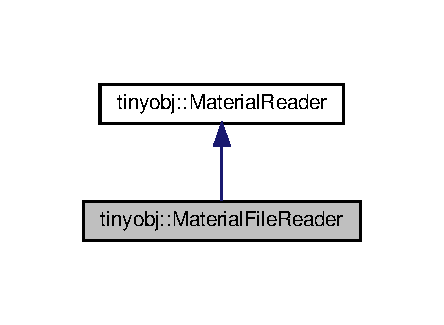
\includegraphics[width=213pt]{classtinyobj_1_1MaterialFileReader__inherit__graph}
\end{center}
\end{figure}


Klasni dijagram za tinyobj\+:\+:Material\+File\+Reader\+:\nopagebreak
\begin{figure}[H]
\begin{center}
\leavevmode
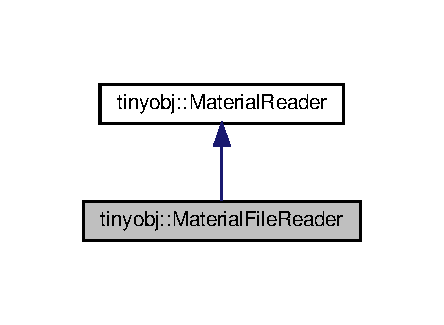
\includegraphics[width=213pt]{classtinyobj_1_1MaterialFileReader__coll__graph}
\end{center}
\end{figure}
\subsection*{Javni članovi}
\begin{DoxyCompactItemize}
\item 
\hyperlink{classtinyobj_1_1MaterialFileReader_aeb0c6d0e32d7876394e570a7b18adc8a}{Material\+File\+Reader} (const std\+::string \&mtl\+\_\+basedir)
\item 
virtual \hyperlink{classtinyobj_1_1MaterialFileReader_a0a00d236393f9972b676a2fb6fe2b819}{$\sim$\+Material\+File\+Reader} ()
\item 
virtual bool \hyperlink{classtinyobj_1_1MaterialFileReader_a23fa55532224cbcc927233f4b57f53df}{operator()} (const std\+::string \&mat\+Id, std\+::vector$<$ \hyperlink{structtinyobj_1_1material__t}{material\+\_\+t} $>$ $\ast$materials, std\+::map$<$ std\+::string, int $>$ $\ast$mat\+Map, std\+::string $\ast$err)
\end{DoxyCompactItemize}
\subsection*{Privatni članovi}
\begin{DoxyCompactItemize}
\item 
std\+::string \hyperlink{classtinyobj_1_1MaterialFileReader_aeb0081a32915ccf6c5c0612335eef560}{m\+\_\+mtl\+Base\+Dir}
\end{DoxyCompactItemize}


\subsection{Dokumentacija konstruktora i destruktora}
\mbox{\Hypertarget{classtinyobj_1_1MaterialFileReader_aeb0c6d0e32d7876394e570a7b18adc8a}\label{classtinyobj_1_1MaterialFileReader_aeb0c6d0e32d7876394e570a7b18adc8a}} 
\index{tinyobj\+::\+Material\+File\+Reader@{tinyobj\+::\+Material\+File\+Reader}!Material\+File\+Reader@{Material\+File\+Reader}}
\index{Material\+File\+Reader@{Material\+File\+Reader}!tinyobj\+::\+Material\+File\+Reader@{tinyobj\+::\+Material\+File\+Reader}}
\subsubsection{\texorpdfstring{Material\+File\+Reader()}{MaterialFileReader()}}
{\footnotesize\ttfamily tinyobj\+::\+Material\+File\+Reader\+::\+Material\+File\+Reader (\begin{DoxyParamCaption}\item[{const std\+::string \&}]{mtl\+\_\+basedir }\end{DoxyParamCaption})\hspace{0.3cm}{\ttfamily [inline]}, {\ttfamily [explicit]}}

\mbox{\Hypertarget{classtinyobj_1_1MaterialFileReader_a0a00d236393f9972b676a2fb6fe2b819}\label{classtinyobj_1_1MaterialFileReader_a0a00d236393f9972b676a2fb6fe2b819}} 
\index{tinyobj\+::\+Material\+File\+Reader@{tinyobj\+::\+Material\+File\+Reader}!````~Material\+File\+Reader@{$\sim$\+Material\+File\+Reader}}
\index{````~Material\+File\+Reader@{$\sim$\+Material\+File\+Reader}!tinyobj\+::\+Material\+File\+Reader@{tinyobj\+::\+Material\+File\+Reader}}
\subsubsection{\texorpdfstring{$\sim$\+Material\+File\+Reader()}{~MaterialFileReader()}}
{\footnotesize\ttfamily virtual tinyobj\+::\+Material\+File\+Reader\+::$\sim$\+Material\+File\+Reader (\begin{DoxyParamCaption}{ }\end{DoxyParamCaption})\hspace{0.3cm}{\ttfamily [inline]}, {\ttfamily [virtual]}}



\subsection{Dokumentacija funkcija članica}
\mbox{\Hypertarget{classtinyobj_1_1MaterialFileReader_a23fa55532224cbcc927233f4b57f53df}\label{classtinyobj_1_1MaterialFileReader_a23fa55532224cbcc927233f4b57f53df}} 
\index{tinyobj\+::\+Material\+File\+Reader@{tinyobj\+::\+Material\+File\+Reader}!operator()@{operator()}}
\index{operator()@{operator()}!tinyobj\+::\+Material\+File\+Reader@{tinyobj\+::\+Material\+File\+Reader}}
\subsubsection{\texorpdfstring{operator()()}{operator()()}}
{\footnotesize\ttfamily virtual bool tinyobj\+::\+Material\+File\+Reader\+::operator() (\begin{DoxyParamCaption}\item[{const std\+::string \&}]{mat\+Id,  }\item[{std\+::vector$<$ \hyperlink{structtinyobj_1_1material__t}{material\+\_\+t} $>$ $\ast$}]{materials,  }\item[{std\+::map$<$ std\+::string, int $>$ $\ast$}]{mat\+Map,  }\item[{std\+::string $\ast$}]{err }\end{DoxyParamCaption})\hspace{0.3cm}{\ttfamily [virtual]}}







\subsection{Dokumentacija atributa}
\mbox{\Hypertarget{classtinyobj_1_1MaterialFileReader_aeb0081a32915ccf6c5c0612335eef560}\label{classtinyobj_1_1MaterialFileReader_aeb0081a32915ccf6c5c0612335eef560}} 
\index{tinyobj\+::\+Material\+File\+Reader@{tinyobj\+::\+Material\+File\+Reader}!m\+\_\+mtl\+Base\+Dir@{m\+\_\+mtl\+Base\+Dir}}
\index{m\+\_\+mtl\+Base\+Dir@{m\+\_\+mtl\+Base\+Dir}!tinyobj\+::\+Material\+File\+Reader@{tinyobj\+::\+Material\+File\+Reader}}
\subsubsection{\texorpdfstring{m\+\_\+mtl\+Base\+Dir}{m\_mtlBaseDir}}
{\footnotesize\ttfamily std\+::string tinyobj\+::\+Material\+File\+Reader\+::m\+\_\+mtl\+Base\+Dir\hspace{0.3cm}{\ttfamily [private]}}



Dokumentacija ove klase je napravljena na osnovu datoteke \begin{DoxyCompactItemize}
\item 
/home/dusan/\+Documents/\+R\+G146-\/vitez-\/reda-\/zmaja/include/external\+\_\+libs/\hyperlink{tiny__obj__loader_8h}{tiny\+\_\+obj\+\_\+loader.\+h}\end{DoxyCompactItemize}

\hypertarget{classtinyobj_1_1MaterialReader}{}\section{Dokumentacija klase tinyobj\+:\+:Material\+Reader}
\label{classtinyobj_1_1MaterialReader}\index{tinyobj\+::\+Material\+Reader@{tinyobj\+::\+Material\+Reader}}


{\ttfamily \#include $<$tiny\+\_\+obj\+\_\+loader.\+h$>$}



Dijagram nasleđivanja za klasu tinyobj\+:\+:Material\+Reader\+:\nopagebreak
\begin{figure}[H]
\begin{center}
\leavevmode
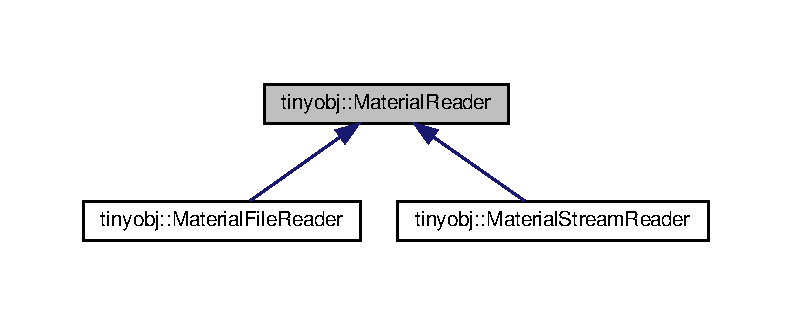
\includegraphics[width=350pt]{classtinyobj_1_1MaterialReader__inherit__graph}
\end{center}
\end{figure}
\subsection*{Javni članovi}
\begin{DoxyCompactItemize}
\item 
\hyperlink{classtinyobj_1_1MaterialReader_a701bdd6217518e0afb5596fcb59925b6}{Material\+Reader} ()
\item 
virtual \hyperlink{classtinyobj_1_1MaterialReader_afd62ceccd9b373801226e037ea1a5f9f}{$\sim$\+Material\+Reader} ()
\item 
virtual bool \hyperlink{classtinyobj_1_1MaterialReader_ad165d8cc1bd989f8548a9258b0881a89}{operator()} (const std\+::string \&mat\+Id, std\+::vector$<$ \hyperlink{structtinyobj_1_1material__t}{material\+\_\+t} $>$ $\ast$materials, std\+::map$<$ std\+::string, int $>$ $\ast$mat\+Map, std\+::string $\ast$err)=0
\end{DoxyCompactItemize}


\subsection{Dokumentacija konstruktora i destruktora}
\mbox{\Hypertarget{classtinyobj_1_1MaterialReader_a701bdd6217518e0afb5596fcb59925b6}\label{classtinyobj_1_1MaterialReader_a701bdd6217518e0afb5596fcb59925b6}} 
\index{tinyobj\+::\+Material\+Reader@{tinyobj\+::\+Material\+Reader}!Material\+Reader@{Material\+Reader}}
\index{Material\+Reader@{Material\+Reader}!tinyobj\+::\+Material\+Reader@{tinyobj\+::\+Material\+Reader}}
\subsubsection{\texorpdfstring{Material\+Reader()}{MaterialReader()}}
{\footnotesize\ttfamily tinyobj\+::\+Material\+Reader\+::\+Material\+Reader (\begin{DoxyParamCaption}{ }\end{DoxyParamCaption})\hspace{0.3cm}{\ttfamily [inline]}}

\mbox{\Hypertarget{classtinyobj_1_1MaterialReader_afd62ceccd9b373801226e037ea1a5f9f}\label{classtinyobj_1_1MaterialReader_afd62ceccd9b373801226e037ea1a5f9f}} 
\index{tinyobj\+::\+Material\+Reader@{tinyobj\+::\+Material\+Reader}!````~Material\+Reader@{$\sim$\+Material\+Reader}}
\index{````~Material\+Reader@{$\sim$\+Material\+Reader}!tinyobj\+::\+Material\+Reader@{tinyobj\+::\+Material\+Reader}}
\subsubsection{\texorpdfstring{$\sim$\+Material\+Reader()}{~MaterialReader()}}
{\footnotesize\ttfamily virtual tinyobj\+::\+Material\+Reader\+::$\sim$\+Material\+Reader (\begin{DoxyParamCaption}{ }\end{DoxyParamCaption})\hspace{0.3cm}{\ttfamily [virtual]}}



\subsection{Dokumentacija funkcija članica}
\mbox{\Hypertarget{classtinyobj_1_1MaterialReader_ad165d8cc1bd989f8548a9258b0881a89}\label{classtinyobj_1_1MaterialReader_ad165d8cc1bd989f8548a9258b0881a89}} 
\index{tinyobj\+::\+Material\+Reader@{tinyobj\+::\+Material\+Reader}!operator()@{operator()}}
\index{operator()@{operator()}!tinyobj\+::\+Material\+Reader@{tinyobj\+::\+Material\+Reader}}
\subsubsection{\texorpdfstring{operator()()}{operator()()}}
{\footnotesize\ttfamily virtual bool tinyobj\+::\+Material\+Reader\+::operator() (\begin{DoxyParamCaption}\item[{const std\+::string \&}]{mat\+Id,  }\item[{std\+::vector$<$ \hyperlink{structtinyobj_1_1material__t}{material\+\_\+t} $>$ $\ast$}]{materials,  }\item[{std\+::map$<$ std\+::string, int $>$ $\ast$}]{mat\+Map,  }\item[{std\+::string $\ast$}]{err }\end{DoxyParamCaption})\hspace{0.3cm}{\ttfamily [pure virtual]}}



Definicija u 



Dokumentacija ove klase je napravljena na osnovu datoteke \begin{DoxyCompactItemize}
\item 
/home/dusan/\+Documents/\+R\+G146-\/vitez-\/reda-\/zmaja/include/external\+\_\+libs/\hyperlink{tiny__obj__loader_8h}{tiny\+\_\+obj\+\_\+loader.\+h}\end{DoxyCompactItemize}

\hypertarget{classtinyobj_1_1MaterialStreamReader}{}\section{Dokumentacija klase tinyobj\+:\+:Material\+Stream\+Reader}
\label{classtinyobj_1_1MaterialStreamReader}\index{tinyobj\+::\+Material\+Stream\+Reader@{tinyobj\+::\+Material\+Stream\+Reader}}


{\ttfamily \#include $<$tiny\+\_\+obj\+\_\+loader.\+h$>$}



Dijagram nasleđivanja za klasu tinyobj\+:\+:Material\+Stream\+Reader\+:
\nopagebreak
\begin{figure}[H]
\begin{center}
\leavevmode
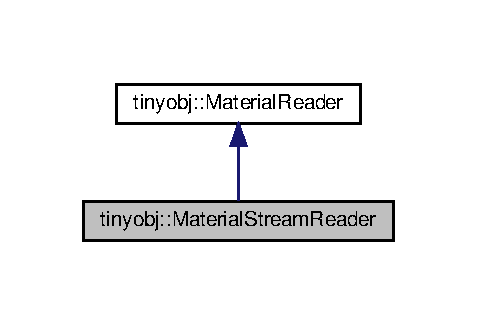
\includegraphics[width=229pt]{classtinyobj_1_1MaterialStreamReader__inherit__graph}
\end{center}
\end{figure}


Klasni dijagram za tinyobj\+:\+:Material\+Stream\+Reader\+:
\nopagebreak
\begin{figure}[H]
\begin{center}
\leavevmode
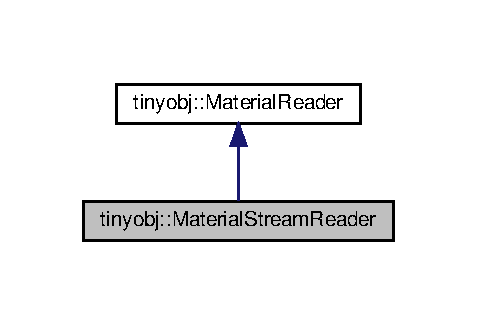
\includegraphics[width=229pt]{classtinyobj_1_1MaterialStreamReader__coll__graph}
\end{center}
\end{figure}
\subsection*{Javni članovi}
\begin{DoxyCompactItemize}
\item 
\hyperlink{classtinyobj_1_1MaterialStreamReader_a6a6b7167e62d239cb3b002b6aa183773}{Material\+Stream\+Reader} (std\+::istream \&in\+Stream)
\item 
virtual \hyperlink{classtinyobj_1_1MaterialStreamReader_afcafa6030bbf8ea8fdbc6aefb8bebc74}{$\sim$\+Material\+Stream\+Reader} ()
\item 
virtual bool \hyperlink{classtinyobj_1_1MaterialStreamReader_a38db9ec731ad3177efa704d7e60c82fd}{operator()} (const std\+::string \&mat\+Id, std\+::vector$<$ \hyperlink{structtinyobj_1_1material__t}{material\+\_\+t} $>$ $\ast$materials, std\+::map$<$ std\+::string, int $>$ $\ast$mat\+Map, std\+::string $\ast$err)
\end{DoxyCompactItemize}
\subsection*{Privatni članovi}
\begin{DoxyCompactItemize}
\item 
std\+::istream \& \hyperlink{classtinyobj_1_1MaterialStreamReader_a8de39704770b77d36d6cebe09d941435}{m\+\_\+in\+Stream}
\end{DoxyCompactItemize}


\subsection{Dokumentacija konstruktora i destruktora}
\mbox{\Hypertarget{classtinyobj_1_1MaterialStreamReader_a6a6b7167e62d239cb3b002b6aa183773}\label{classtinyobj_1_1MaterialStreamReader_a6a6b7167e62d239cb3b002b6aa183773}} 
\index{tinyobj\+::\+Material\+Stream\+Reader@{tinyobj\+::\+Material\+Stream\+Reader}!Material\+Stream\+Reader@{Material\+Stream\+Reader}}
\index{Material\+Stream\+Reader@{Material\+Stream\+Reader}!tinyobj\+::\+Material\+Stream\+Reader@{tinyobj\+::\+Material\+Stream\+Reader}}
\subsubsection{\texorpdfstring{Material\+Stream\+Reader()}{MaterialStreamReader()}}
{\footnotesize\ttfamily tinyobj\+::\+Material\+Stream\+Reader\+::\+Material\+Stream\+Reader (\begin{DoxyParamCaption}\item[{std\+::istream \&}]{in\+Stream }\end{DoxyParamCaption})\hspace{0.3cm}{\ttfamily [inline]}, {\ttfamily [explicit]}}

\mbox{\Hypertarget{classtinyobj_1_1MaterialStreamReader_afcafa6030bbf8ea8fdbc6aefb8bebc74}\label{classtinyobj_1_1MaterialStreamReader_afcafa6030bbf8ea8fdbc6aefb8bebc74}} 
\index{tinyobj\+::\+Material\+Stream\+Reader@{tinyobj\+::\+Material\+Stream\+Reader}!````~Material\+Stream\+Reader@{$\sim$\+Material\+Stream\+Reader}}
\index{````~Material\+Stream\+Reader@{$\sim$\+Material\+Stream\+Reader}!tinyobj\+::\+Material\+Stream\+Reader@{tinyobj\+::\+Material\+Stream\+Reader}}
\subsubsection{\texorpdfstring{$\sim$\+Material\+Stream\+Reader()}{~MaterialStreamReader()}}
{\footnotesize\ttfamily virtual tinyobj\+::\+Material\+Stream\+Reader\+::$\sim$\+Material\+Stream\+Reader (\begin{DoxyParamCaption}{ }\end{DoxyParamCaption})\hspace{0.3cm}{\ttfamily [inline]}, {\ttfamily [virtual]}}



\subsection{Dokumentacija funkcija članica}
\mbox{\Hypertarget{classtinyobj_1_1MaterialStreamReader_a38db9ec731ad3177efa704d7e60c82fd}\label{classtinyobj_1_1MaterialStreamReader_a38db9ec731ad3177efa704d7e60c82fd}} 
\index{tinyobj\+::\+Material\+Stream\+Reader@{tinyobj\+::\+Material\+Stream\+Reader}!operator()@{operator()}}
\index{operator()@{operator()}!tinyobj\+::\+Material\+Stream\+Reader@{tinyobj\+::\+Material\+Stream\+Reader}}
\subsubsection{\texorpdfstring{operator()()}{operator()()}}
{\footnotesize\ttfamily virtual bool tinyobj\+::\+Material\+Stream\+Reader\+::operator() (\begin{DoxyParamCaption}\item[{const std\+::string \&}]{mat\+Id,  }\item[{std\+::vector$<$ \hyperlink{structtinyobj_1_1material__t}{material\+\_\+t} $>$ $\ast$}]{materials,  }\item[{std\+::map$<$ std\+::string, int $>$ $\ast$}]{mat\+Map,  }\item[{std\+::string $\ast$}]{err }\end{DoxyParamCaption})\hspace{0.3cm}{\ttfamily [virtual]}}







\subsection{Dokumentacija atributa}
\mbox{\Hypertarget{classtinyobj_1_1MaterialStreamReader_a8de39704770b77d36d6cebe09d941435}\label{classtinyobj_1_1MaterialStreamReader_a8de39704770b77d36d6cebe09d941435}} 
\index{tinyobj\+::\+Material\+Stream\+Reader@{tinyobj\+::\+Material\+Stream\+Reader}!m\+\_\+in\+Stream@{m\+\_\+in\+Stream}}
\index{m\+\_\+in\+Stream@{m\+\_\+in\+Stream}!tinyobj\+::\+Material\+Stream\+Reader@{tinyobj\+::\+Material\+Stream\+Reader}}
\subsubsection{\texorpdfstring{m\+\_\+in\+Stream}{m\_inStream}}
{\footnotesize\ttfamily std\+::istream\& tinyobj\+::\+Material\+Stream\+Reader\+::m\+\_\+in\+Stream\hspace{0.3cm}{\ttfamily [private]}}



Dokumentacija ove klase je napravljena na osnovu datoteke \begin{DoxyCompactItemize}
\item 
/home/dusan/\+Documents/\+Projects/\+R\+G102-\/vitez-\/reda-\/zmaja/include/external\+\_\+libs/\hyperlink{tiny__obj__loader_8h}{tiny\+\_\+obj\+\_\+loader.\+h}\end{DoxyCompactItemize}

\hypertarget{structtinyobj_1_1mesh__t}{}\section{Dokumentacija strukture tinyobj\+:\+:mesh\+\_\+t}
\label{structtinyobj_1_1mesh__t}\index{tinyobj\+::mesh\+\_\+t@{tinyobj\+::mesh\+\_\+t}}


{\ttfamily \#include $<$tiny\+\_\+obj\+\_\+loader.\+h$>$}

\subsection*{Javni članovi}
\begin{DoxyCompactItemize}
\item 
std\+::vector$<$ \hyperlink{structtinyobj_1_1index__t}{index\+\_\+t} $>$ \hyperlink{structtinyobj_1_1mesh__t_a9dcdbdf04eca02a552793ac7d160127c}{indices}
\item 
std\+::vector$<$ unsigned char $>$ \hyperlink{structtinyobj_1_1mesh__t_ae5f29bef4c1de10253020f9f7ab7374e}{num\+\_\+face\+\_\+vertices}
\item 
std\+::vector$<$ int $>$ \hyperlink{structtinyobj_1_1mesh__t_a57b2f12dfa3fd620b25babcd3a09ec6b}{material\+\_\+ids}
\item 
std\+::vector$<$ unsigned int $>$ \hyperlink{structtinyobj_1_1mesh__t_a89b017a3446709c264d94438a9d7541b}{smoothing\+\_\+group\+\_\+ids}
\item 
std\+::vector$<$ \hyperlink{structtinyobj_1_1tag__t}{tag\+\_\+t} $>$ \hyperlink{structtinyobj_1_1mesh__t_a60f51d3802c11e2bf269530e0337fc63}{tags}
\end{DoxyCompactItemize}


\subsection{Dokumentacija atributa}
\mbox{\Hypertarget{structtinyobj_1_1mesh__t_a9dcdbdf04eca02a552793ac7d160127c}\label{structtinyobj_1_1mesh__t_a9dcdbdf04eca02a552793ac7d160127c}} 
\index{tinyobj\+::mesh\+\_\+t@{tinyobj\+::mesh\+\_\+t}!indices@{indices}}
\index{indices@{indices}!tinyobj\+::mesh\+\_\+t@{tinyobj\+::mesh\+\_\+t}}
\subsubsection{\texorpdfstring{indices}{indices}}
{\footnotesize\ttfamily std\+::vector$<$\hyperlink{structtinyobj_1_1index__t}{index\+\_\+t}$>$ tinyobj\+::mesh\+\_\+t\+::indices}

\mbox{\Hypertarget{structtinyobj_1_1mesh__t_a57b2f12dfa3fd620b25babcd3a09ec6b}\label{structtinyobj_1_1mesh__t_a57b2f12dfa3fd620b25babcd3a09ec6b}} 
\index{tinyobj\+::mesh\+\_\+t@{tinyobj\+::mesh\+\_\+t}!material\+\_\+ids@{material\+\_\+ids}}
\index{material\+\_\+ids@{material\+\_\+ids}!tinyobj\+::mesh\+\_\+t@{tinyobj\+::mesh\+\_\+t}}
\subsubsection{\texorpdfstring{material\+\_\+ids}{material\_ids}}
{\footnotesize\ttfamily std\+::vector$<$int$>$ tinyobj\+::mesh\+\_\+t\+::material\+\_\+ids}

\mbox{\Hypertarget{structtinyobj_1_1mesh__t_ae5f29bef4c1de10253020f9f7ab7374e}\label{structtinyobj_1_1mesh__t_ae5f29bef4c1de10253020f9f7ab7374e}} 
\index{tinyobj\+::mesh\+\_\+t@{tinyobj\+::mesh\+\_\+t}!num\+\_\+face\+\_\+vertices@{num\+\_\+face\+\_\+vertices}}
\index{num\+\_\+face\+\_\+vertices@{num\+\_\+face\+\_\+vertices}!tinyobj\+::mesh\+\_\+t@{tinyobj\+::mesh\+\_\+t}}
\subsubsection{\texorpdfstring{num\+\_\+face\+\_\+vertices}{num\_face\_vertices}}
{\footnotesize\ttfamily std\+::vector$<$unsigned char$>$ tinyobj\+::mesh\+\_\+t\+::num\+\_\+face\+\_\+vertices}

\mbox{\Hypertarget{structtinyobj_1_1mesh__t_a89b017a3446709c264d94438a9d7541b}\label{structtinyobj_1_1mesh__t_a89b017a3446709c264d94438a9d7541b}} 
\index{tinyobj\+::mesh\+\_\+t@{tinyobj\+::mesh\+\_\+t}!smoothing\+\_\+group\+\_\+ids@{smoothing\+\_\+group\+\_\+ids}}
\index{smoothing\+\_\+group\+\_\+ids@{smoothing\+\_\+group\+\_\+ids}!tinyobj\+::mesh\+\_\+t@{tinyobj\+::mesh\+\_\+t}}
\subsubsection{\texorpdfstring{smoothing\+\_\+group\+\_\+ids}{smoothing\_group\_ids}}
{\footnotesize\ttfamily std\+::vector$<$unsigned int$>$ tinyobj\+::mesh\+\_\+t\+::smoothing\+\_\+group\+\_\+ids}

\mbox{\Hypertarget{structtinyobj_1_1mesh__t_a60f51d3802c11e2bf269530e0337fc63}\label{structtinyobj_1_1mesh__t_a60f51d3802c11e2bf269530e0337fc63}} 
\index{tinyobj\+::mesh\+\_\+t@{tinyobj\+::mesh\+\_\+t}!tags@{tags}}
\index{tags@{tags}!tinyobj\+::mesh\+\_\+t@{tinyobj\+::mesh\+\_\+t}}
\subsubsection{\texorpdfstring{tags}{tags}}
{\footnotesize\ttfamily std\+::vector$<$\hyperlink{structtinyobj_1_1tag__t}{tag\+\_\+t}$>$ tinyobj\+::mesh\+\_\+t\+::tags}



Dokumentacija ove strukture je napravljena na osnovu datoteke \begin{DoxyCompactItemize}
\item 
/home/dusan/\+Documents/\+R\+G146-\/vitez-\/reda-\/zmaja/include/external\+\_\+libs/\hyperlink{tiny__obj__loader_8h}{tiny\+\_\+obj\+\_\+loader.\+h}\end{DoxyCompactItemize}

\hypertarget{classtexture_1_1ModelTexture}{}\section{Dokumentacija klase texture\+:\+:Model\+Texture}
\label{classtexture_1_1ModelTexture}\index{texture\+::\+Model\+Texture@{texture\+::\+Model\+Texture}}


Klasa Textured\+Model opisuje teksturu objekta. Model je opisan instancom klase Raw\+Model i odgovarajucom teksturom objekta pomocu instance klase \hyperlink{classtexture_1_1ModelTexture}{Model\+Texture}.  




{\ttfamily \#include $<$Model\+Texture.\+h$>$}

\subsection*{Javni članovi}
\begin{DoxyCompactItemize}
\item 
\hyperlink{classtexture_1_1ModelTexture_a8a404382554b8e2625978824202c42b9}{Model\+Texture} (int id)
\begin{DoxyCompactList}\small\item\em Konstruktor klase. U konstruktoru se dodeljuje identifikator teksture ucitana iz png fajla. \end{DoxyCompactList}\item 
\hyperlink{classtexture_1_1ModelTexture_ab0ce63043b8241b064a2c233ec24bfae}{$\sim$\+Model\+Texture} ()
\begin{DoxyCompactList}\small\item\em Destruktor klase. \end{DoxyCompactList}\item 
int \hyperlink{classtexture_1_1ModelTexture_a3eeda8235d9c4cfccccc2ac805eeb864}{get\+ID} ()
\begin{DoxyCompactList}\small\item\em Funkcija vraca identifikator teksture. \end{DoxyCompactList}\item 
float \hyperlink{classtexture_1_1ModelTexture_a2336ba8c1ccc1eea9419fb2cd3773888}{get\+Shine} ()
\begin{DoxyCompactList}\small\item\em Funkcija vraca intenzitet sjaja. \end{DoxyCompactList}\item 
float \hyperlink{classtexture_1_1ModelTexture_a613024c969ec176a1add0c20c3f98969}{get\+Reflectivity} ()
\begin{DoxyCompactList}\small\item\em Funkcija vraca intenzitet reflektovanja. \end{DoxyCompactList}\item 
bool \hyperlink{classtexture_1_1ModelTexture_adc0735b6b9c1df9f2c525f0663306cd3}{get\+Has\+Transparency} ()
\begin{DoxyCompactList}\small\item\em Funkcija vraca prozirnost. \end{DoxyCompactList}\item 
bool \hyperlink{classtexture_1_1ModelTexture_adc202fd47232d085312fea26bc17d69e}{get\+Use\+Fake\+Lightning} ()
\begin{DoxyCompactList}\small\item\em Funkcija vraca koriscenje laznog osvetljenja. \end{DoxyCompactList}\item 
void \hyperlink{classtexture_1_1ModelTexture_a782076c3a92f7d92cd45a92c5ef088a1}{set\+Shine} (float \hyperlink{classtexture_1_1ModelTexture_a7a74ed6a4d5fc91d1537fbf68e74ce03}{shine})
\begin{DoxyCompactList}\small\item\em Funkcija postavlja intenzitet sjaja. \end{DoxyCompactList}\item 
void \hyperlink{classtexture_1_1ModelTexture_a87d88c1857f107c1169b24d1488f5cbc}{set\+Reflectivity} (float \hyperlink{classtexture_1_1ModelTexture_a230e6f2abbfc59eae1daf72eba177b90}{reflectivity})
\begin{DoxyCompactList}\small\item\em Funkcija postavlja intenzitet reflektovanja. \end{DoxyCompactList}\item 
void \hyperlink{classtexture_1_1ModelTexture_a04240906ba55ecaaec9a793788da9c58}{set\+Has\+Transparency} (bool transparency)
\begin{DoxyCompactList}\small\item\em Funkcija postavlja prozirnost. \end{DoxyCompactList}\item 
void \hyperlink{classtexture_1_1ModelTexture_a616d99807f2487d6723380ec03b57ede}{set\+Use\+Fake\+Lightning} (bool lightning)
\begin{DoxyCompactList}\small\item\em Funkcija postavlja koriscenje laznog osvetljenja. \end{DoxyCompactList}\end{DoxyCompactItemize}
\subsection*{Privatni članovi}
\begin{DoxyCompactItemize}
\item 
int \hyperlink{classtexture_1_1ModelTexture_a0dca1304604e6b705acb0460b66fce36}{texture\+ID}
\begin{DoxyCompactList}\small\item\em Identifikator teksture. \end{DoxyCompactList}\item 
float \hyperlink{classtexture_1_1ModelTexture_a7a74ed6a4d5fc91d1537fbf68e74ce03}{shine}
\begin{DoxyCompactList}\small\item\em Intenzitet sjaja. \end{DoxyCompactList}\item 
float \hyperlink{classtexture_1_1ModelTexture_a230e6f2abbfc59eae1daf72eba177b90}{reflectivity}
\begin{DoxyCompactList}\small\item\em Intenzitet reflektovanja svetlosti. \end{DoxyCompactList}\item 
bool \hyperlink{classtexture_1_1ModelTexture_add1146be92d76ac599fa032117e8b459}{has\+Transparency}
\begin{DoxyCompactList}\small\item\em Providnost. \end{DoxyCompactList}\item 
bool \hyperlink{classtexture_1_1ModelTexture_aa14650f7cc629b9f5c0ed15f82b22cad}{use\+Fake\+Lightning}
\begin{DoxyCompactList}\small\item\em Koriscenje laznog osvetljenja. \end{DoxyCompactList}\end{DoxyCompactItemize}


\subsection{Opširniji opis}
Klasa Textured\+Model opisuje teksturu objekta. Model je opisan instancom klase Raw\+Model i odgovarajucom teksturom objekta pomocu instance klase \hyperlink{classtexture_1_1ModelTexture}{Model\+Texture}. 

\subsection{Dokumentacija konstruktora i destruktora}
\mbox{\Hypertarget{classtexture_1_1ModelTexture_a8a404382554b8e2625978824202c42b9}\label{classtexture_1_1ModelTexture_a8a404382554b8e2625978824202c42b9}} 
\index{texture\+::\+Model\+Texture@{texture\+::\+Model\+Texture}!Model\+Texture@{Model\+Texture}}
\index{Model\+Texture@{Model\+Texture}!texture\+::\+Model\+Texture@{texture\+::\+Model\+Texture}}
\subsubsection{\texorpdfstring{Model\+Texture()}{ModelTexture()}}
{\footnotesize\ttfamily texture\+::\+Model\+Texture\+::\+Model\+Texture (\begin{DoxyParamCaption}\item[{int}]{id }\end{DoxyParamCaption})}



Konstruktor klase. U konstruktoru se dodeljuje identifikator teksture ucitana iz png fajla. 


\begin{DoxyParams}{Parametri}
{\em id} & Identifikator teksture. \\
\hline
\end{DoxyParams}
\mbox{\Hypertarget{classtexture_1_1ModelTexture_ab0ce63043b8241b064a2c233ec24bfae}\label{classtexture_1_1ModelTexture_ab0ce63043b8241b064a2c233ec24bfae}} 
\index{texture\+::\+Model\+Texture@{texture\+::\+Model\+Texture}!````~Model\+Texture@{$\sim$\+Model\+Texture}}
\index{````~Model\+Texture@{$\sim$\+Model\+Texture}!texture\+::\+Model\+Texture@{texture\+::\+Model\+Texture}}
\subsubsection{\texorpdfstring{$\sim$\+Model\+Texture()}{~ModelTexture()}}
{\footnotesize\ttfamily texture\+::\+Model\+Texture\+::$\sim$\+Model\+Texture (\begin{DoxyParamCaption}{ }\end{DoxyParamCaption})}



Destruktor klase. 


\begin{DoxyParams}{Parametri}
{\em void} & \\
\hline
\end{DoxyParams}


\subsection{Dokumentacija funkcija članica}
\mbox{\Hypertarget{classtexture_1_1ModelTexture_adc0735b6b9c1df9f2c525f0663306cd3}\label{classtexture_1_1ModelTexture_adc0735b6b9c1df9f2c525f0663306cd3}} 
\index{texture\+::\+Model\+Texture@{texture\+::\+Model\+Texture}!get\+Has\+Transparency@{get\+Has\+Transparency}}
\index{get\+Has\+Transparency@{get\+Has\+Transparency}!texture\+::\+Model\+Texture@{texture\+::\+Model\+Texture}}
\subsubsection{\texorpdfstring{get\+Has\+Transparency()}{getHasTransparency()}}
{\footnotesize\ttfamily bool texture\+::\+Model\+Texture\+::get\+Has\+Transparency (\begin{DoxyParamCaption}{ }\end{DoxyParamCaption})}



Funkcija vraca prozirnost. 


\begin{DoxyParams}{Parametri}
{\em void} & \\
\hline
\end{DoxyParams}
\begin{DoxyReturn}{Vrednost funkcije}
bool Prozirnost. 
\end{DoxyReturn}
\mbox{\Hypertarget{classtexture_1_1ModelTexture_a3eeda8235d9c4cfccccc2ac805eeb864}\label{classtexture_1_1ModelTexture_a3eeda8235d9c4cfccccc2ac805eeb864}} 
\index{texture\+::\+Model\+Texture@{texture\+::\+Model\+Texture}!get\+ID@{get\+ID}}
\index{get\+ID@{get\+ID}!texture\+::\+Model\+Texture@{texture\+::\+Model\+Texture}}
\subsubsection{\texorpdfstring{get\+I\+D()}{getID()}}
{\footnotesize\ttfamily int texture\+::\+Model\+Texture\+::get\+ID (\begin{DoxyParamCaption}{ }\end{DoxyParamCaption})}



Funkcija vraca identifikator teksture. 


\begin{DoxyParams}{Parametri}
{\em void} & \\
\hline
\end{DoxyParams}
\begin{DoxyReturn}{Vrednost funkcije}
int Identifikator teksture. 
\end{DoxyReturn}
\mbox{\Hypertarget{classtexture_1_1ModelTexture_a613024c969ec176a1add0c20c3f98969}\label{classtexture_1_1ModelTexture_a613024c969ec176a1add0c20c3f98969}} 
\index{texture\+::\+Model\+Texture@{texture\+::\+Model\+Texture}!get\+Reflectivity@{get\+Reflectivity}}
\index{get\+Reflectivity@{get\+Reflectivity}!texture\+::\+Model\+Texture@{texture\+::\+Model\+Texture}}
\subsubsection{\texorpdfstring{get\+Reflectivity()}{getReflectivity()}}
{\footnotesize\ttfamily float texture\+::\+Model\+Texture\+::get\+Reflectivity (\begin{DoxyParamCaption}{ }\end{DoxyParamCaption})}



Funkcija vraca intenzitet reflektovanja. 


\begin{DoxyParams}{Parametri}
{\em void} & \\
\hline
\end{DoxyParams}
\begin{DoxyReturn}{Vrednost funkcije}
float Intenzitet reflektovanja. 
\end{DoxyReturn}
\mbox{\Hypertarget{classtexture_1_1ModelTexture_a2336ba8c1ccc1eea9419fb2cd3773888}\label{classtexture_1_1ModelTexture_a2336ba8c1ccc1eea9419fb2cd3773888}} 
\index{texture\+::\+Model\+Texture@{texture\+::\+Model\+Texture}!get\+Shine@{get\+Shine}}
\index{get\+Shine@{get\+Shine}!texture\+::\+Model\+Texture@{texture\+::\+Model\+Texture}}
\subsubsection{\texorpdfstring{get\+Shine()}{getShine()}}
{\footnotesize\ttfamily float texture\+::\+Model\+Texture\+::get\+Shine (\begin{DoxyParamCaption}{ }\end{DoxyParamCaption})}



Funkcija vraca intenzitet sjaja. 


\begin{DoxyParams}{Parametri}
{\em void} & \\
\hline
\end{DoxyParams}
\begin{DoxyReturn}{Vrednost funkcije}
float Intenzitet sjaja. 
\end{DoxyReturn}
\mbox{\Hypertarget{classtexture_1_1ModelTexture_adc202fd47232d085312fea26bc17d69e}\label{classtexture_1_1ModelTexture_adc202fd47232d085312fea26bc17d69e}} 
\index{texture\+::\+Model\+Texture@{texture\+::\+Model\+Texture}!get\+Use\+Fake\+Lightning@{get\+Use\+Fake\+Lightning}}
\index{get\+Use\+Fake\+Lightning@{get\+Use\+Fake\+Lightning}!texture\+::\+Model\+Texture@{texture\+::\+Model\+Texture}}
\subsubsection{\texorpdfstring{get\+Use\+Fake\+Lightning()}{getUseFakeLightning()}}
{\footnotesize\ttfamily bool texture\+::\+Model\+Texture\+::get\+Use\+Fake\+Lightning (\begin{DoxyParamCaption}{ }\end{DoxyParamCaption})}



Funkcija vraca koriscenje laznog osvetljenja. 


\begin{DoxyParams}{Parametri}
{\em void} & \\
\hline
\end{DoxyParams}
\begin{DoxyReturn}{Vrednost funkcije}
bool Koriscenje laznog osvetljenja. 
\end{DoxyReturn}
\mbox{\Hypertarget{classtexture_1_1ModelTexture_a04240906ba55ecaaec9a793788da9c58}\label{classtexture_1_1ModelTexture_a04240906ba55ecaaec9a793788da9c58}} 
\index{texture\+::\+Model\+Texture@{texture\+::\+Model\+Texture}!set\+Has\+Transparency@{set\+Has\+Transparency}}
\index{set\+Has\+Transparency@{set\+Has\+Transparency}!texture\+::\+Model\+Texture@{texture\+::\+Model\+Texture}}
\subsubsection{\texorpdfstring{set\+Has\+Transparency()}{setHasTransparency()}}
{\footnotesize\ttfamily void texture\+::\+Model\+Texture\+::set\+Has\+Transparency (\begin{DoxyParamCaption}\item[{bool}]{transparency }\end{DoxyParamCaption})}



Funkcija postavlja prozirnost. 


\begin{DoxyParams}{Parametri}
{\em transparency} & Prozirnost. \\
\hline
\end{DoxyParams}
\begin{DoxyReturn}{Vrednost funkcije}
void 
\end{DoxyReturn}
\mbox{\Hypertarget{classtexture_1_1ModelTexture_a87d88c1857f107c1169b24d1488f5cbc}\label{classtexture_1_1ModelTexture_a87d88c1857f107c1169b24d1488f5cbc}} 
\index{texture\+::\+Model\+Texture@{texture\+::\+Model\+Texture}!set\+Reflectivity@{set\+Reflectivity}}
\index{set\+Reflectivity@{set\+Reflectivity}!texture\+::\+Model\+Texture@{texture\+::\+Model\+Texture}}
\subsubsection{\texorpdfstring{set\+Reflectivity()}{setReflectivity()}}
{\footnotesize\ttfamily void texture\+::\+Model\+Texture\+::set\+Reflectivity (\begin{DoxyParamCaption}\item[{float}]{reflectivity }\end{DoxyParamCaption})}



Funkcija postavlja intenzitet reflektovanja. 


\begin{DoxyParams}{Parametri}
{\em reflectivity} & Intenzitet reflektovanja. \\
\hline
\end{DoxyParams}
\begin{DoxyReturn}{Vrednost funkcije}
void 
\end{DoxyReturn}
\mbox{\Hypertarget{classtexture_1_1ModelTexture_a782076c3a92f7d92cd45a92c5ef088a1}\label{classtexture_1_1ModelTexture_a782076c3a92f7d92cd45a92c5ef088a1}} 
\index{texture\+::\+Model\+Texture@{texture\+::\+Model\+Texture}!set\+Shine@{set\+Shine}}
\index{set\+Shine@{set\+Shine}!texture\+::\+Model\+Texture@{texture\+::\+Model\+Texture}}
\subsubsection{\texorpdfstring{set\+Shine()}{setShine()}}
{\footnotesize\ttfamily void texture\+::\+Model\+Texture\+::set\+Shine (\begin{DoxyParamCaption}\item[{float}]{shine }\end{DoxyParamCaption})}



Funkcija postavlja intenzitet sjaja. 


\begin{DoxyParams}{Parametri}
{\em shine} & Intenzitet sjaja. \\
\hline
\end{DoxyParams}
\begin{DoxyReturn}{Vrednost funkcije}
void 
\end{DoxyReturn}
\mbox{\Hypertarget{classtexture_1_1ModelTexture_a616d99807f2487d6723380ec03b57ede}\label{classtexture_1_1ModelTexture_a616d99807f2487d6723380ec03b57ede}} 
\index{texture\+::\+Model\+Texture@{texture\+::\+Model\+Texture}!set\+Use\+Fake\+Lightning@{set\+Use\+Fake\+Lightning}}
\index{set\+Use\+Fake\+Lightning@{set\+Use\+Fake\+Lightning}!texture\+::\+Model\+Texture@{texture\+::\+Model\+Texture}}
\subsubsection{\texorpdfstring{set\+Use\+Fake\+Lightning()}{setUseFakeLightning()}}
{\footnotesize\ttfamily void texture\+::\+Model\+Texture\+::set\+Use\+Fake\+Lightning (\begin{DoxyParamCaption}\item[{bool}]{lightning }\end{DoxyParamCaption})}



Funkcija postavlja koriscenje laznog osvetljenja. 


\begin{DoxyParams}{Parametri}
{\em lightning} & Koriscenje laznog osvetljenja. \\
\hline
\end{DoxyParams}
\begin{DoxyReturn}{Vrednost funkcije}
void 
\end{DoxyReturn}


\subsection{Dokumentacija atributa}
\mbox{\Hypertarget{classtexture_1_1ModelTexture_add1146be92d76ac599fa032117e8b459}\label{classtexture_1_1ModelTexture_add1146be92d76ac599fa032117e8b459}} 
\index{texture\+::\+Model\+Texture@{texture\+::\+Model\+Texture}!has\+Transparency@{has\+Transparency}}
\index{has\+Transparency@{has\+Transparency}!texture\+::\+Model\+Texture@{texture\+::\+Model\+Texture}}
\subsubsection{\texorpdfstring{has\+Transparency}{hasTransparency}}
{\footnotesize\ttfamily bool texture\+::\+Model\+Texture\+::has\+Transparency\hspace{0.3cm}{\ttfamily [private]}}



Providnost. 

\mbox{\Hypertarget{classtexture_1_1ModelTexture_a230e6f2abbfc59eae1daf72eba177b90}\label{classtexture_1_1ModelTexture_a230e6f2abbfc59eae1daf72eba177b90}} 
\index{texture\+::\+Model\+Texture@{texture\+::\+Model\+Texture}!reflectivity@{reflectivity}}
\index{reflectivity@{reflectivity}!texture\+::\+Model\+Texture@{texture\+::\+Model\+Texture}}
\subsubsection{\texorpdfstring{reflectivity}{reflectivity}}
{\footnotesize\ttfamily float texture\+::\+Model\+Texture\+::reflectivity\hspace{0.3cm}{\ttfamily [private]}}



Intenzitet reflektovanja svetlosti. 

\mbox{\Hypertarget{classtexture_1_1ModelTexture_a7a74ed6a4d5fc91d1537fbf68e74ce03}\label{classtexture_1_1ModelTexture_a7a74ed6a4d5fc91d1537fbf68e74ce03}} 
\index{texture\+::\+Model\+Texture@{texture\+::\+Model\+Texture}!shine@{shine}}
\index{shine@{shine}!texture\+::\+Model\+Texture@{texture\+::\+Model\+Texture}}
\subsubsection{\texorpdfstring{shine}{shine}}
{\footnotesize\ttfamily float texture\+::\+Model\+Texture\+::shine\hspace{0.3cm}{\ttfamily [private]}}



Intenzitet sjaja. 

\mbox{\Hypertarget{classtexture_1_1ModelTexture_a0dca1304604e6b705acb0460b66fce36}\label{classtexture_1_1ModelTexture_a0dca1304604e6b705acb0460b66fce36}} 
\index{texture\+::\+Model\+Texture@{texture\+::\+Model\+Texture}!texture\+ID@{texture\+ID}}
\index{texture\+ID@{texture\+ID}!texture\+::\+Model\+Texture@{texture\+::\+Model\+Texture}}
\subsubsection{\texorpdfstring{texture\+ID}{textureID}}
{\footnotesize\ttfamily int texture\+::\+Model\+Texture\+::texture\+ID\hspace{0.3cm}{\ttfamily [private]}}



Identifikator teksture. 

\mbox{\Hypertarget{classtexture_1_1ModelTexture_aa14650f7cc629b9f5c0ed15f82b22cad}\label{classtexture_1_1ModelTexture_aa14650f7cc629b9f5c0ed15f82b22cad}} 
\index{texture\+::\+Model\+Texture@{texture\+::\+Model\+Texture}!use\+Fake\+Lightning@{use\+Fake\+Lightning}}
\index{use\+Fake\+Lightning@{use\+Fake\+Lightning}!texture\+::\+Model\+Texture@{texture\+::\+Model\+Texture}}
\subsubsection{\texorpdfstring{use\+Fake\+Lightning}{useFakeLightning}}
{\footnotesize\ttfamily bool texture\+::\+Model\+Texture\+::use\+Fake\+Lightning\hspace{0.3cm}{\ttfamily [private]}}



Koriscenje laznog osvetljenja. 



Dokumentacija ove klase je napravljena na osnovu sledećih datoteka\+:\begin{DoxyCompactItemize}
\item 
/home/dusan/\+Documents/\+R\+G146-\/vitez-\/reda-\/zmaja/include/texture/\hyperlink{ModelTexture_8h}{Model\+Texture.\+h}\item 
/home/dusan/\+Documents/\+R\+G146-\/vitez-\/reda-\/zmaja/src/texture/\hyperlink{ModelTexture_8cpp}{Model\+Texture.\+cpp}\end{DoxyCompactItemize}

\hypertarget{classcore_1_1ObjLoader}{}\section{Dokumentacija klase core\+:\+:Obj\+Loader}
\label{classcore_1_1ObjLoader}\index{core\+::\+Obj\+Loader@{core\+::\+Obj\+Loader}}


Klasa \hyperlink{classcore_1_1ObjLoader}{Obj\+Loader} je zaduzena za ucitavanje obj fajlova. Tokom pokretanja citaju se obj fajlovi koji se zatim obradjuju i podaci se prosledjuju drugim klasama koje ih koriste.  




{\ttfamily \#include $<$Obj\+Loader.\+h$>$}

\subsection*{Javni članovi}
\begin{DoxyCompactItemize}
\item 
\hyperlink{classcore_1_1ObjLoader_a4cdb4b0e2d995d3ea0f51f255e791aaa}{Obj\+Loader} ()
\begin{DoxyCompactList}\small\item\em Konstruktor klase. \end{DoxyCompactList}\item 
\hyperlink{classcore_1_1ObjLoader_a127a52d790309d913f7f3711a5d8c3f4}{$\sim$\+Obj\+Loader} ()
\begin{DoxyCompactList}\small\item\em Destruktor klase. \end{DoxyCompactList}\item 
\hyperlink{classmodel_1_1RawModel}{Raw\+Model} $\ast$ \hyperlink{classcore_1_1ObjLoader_a47f303f773dfbd6d33598a53a1dbcbc4}{load\+Obj\+Model} (const char $\ast$file\+Name, \hyperlink{classcore_1_1VaoLoader}{Vao\+Loader} $\ast$\hyperlink{namespacecore_a78dd24784c415d3759a0f71b8f4f9f81}{vao\+Loader})
\begin{DoxyCompactList}\small\item\em Funkcija ucitava obj fajl i koristi podatke koji su u njemu za generisanje objekta. \end{DoxyCompactList}\end{DoxyCompactItemize}


\subsection{Opširniji opis}
Klasa \hyperlink{classcore_1_1ObjLoader}{Obj\+Loader} je zaduzena za ucitavanje obj fajlova. Tokom pokretanja citaju se obj fajlovi koji se zatim obradjuju i podaci se prosledjuju drugim klasama koje ih koriste. 

\subsection{Dokumentacija konstruktora i destruktora}
\mbox{\Hypertarget{classcore_1_1ObjLoader_a4cdb4b0e2d995d3ea0f51f255e791aaa}\label{classcore_1_1ObjLoader_a4cdb4b0e2d995d3ea0f51f255e791aaa}} 
\index{core\+::\+Obj\+Loader@{core\+::\+Obj\+Loader}!Obj\+Loader@{Obj\+Loader}}
\index{Obj\+Loader@{Obj\+Loader}!core\+::\+Obj\+Loader@{core\+::\+Obj\+Loader}}
\subsubsection{\texorpdfstring{Obj\+Loader()}{ObjLoader()}}
{\footnotesize\ttfamily core\+::\+Obj\+Loader\+::\+Obj\+Loader (\begin{DoxyParamCaption}{ }\end{DoxyParamCaption})}



Konstruktor klase. 


\begin{DoxyParams}{Parametri}
{\em void} & \\
\hline
\end{DoxyParams}
\mbox{\Hypertarget{classcore_1_1ObjLoader_a127a52d790309d913f7f3711a5d8c3f4}\label{classcore_1_1ObjLoader_a127a52d790309d913f7f3711a5d8c3f4}} 
\index{core\+::\+Obj\+Loader@{core\+::\+Obj\+Loader}!````~Obj\+Loader@{$\sim$\+Obj\+Loader}}
\index{````~Obj\+Loader@{$\sim$\+Obj\+Loader}!core\+::\+Obj\+Loader@{core\+::\+Obj\+Loader}}
\subsubsection{\texorpdfstring{$\sim$\+Obj\+Loader()}{~ObjLoader()}}
{\footnotesize\ttfamily core\+::\+Obj\+Loader\+::$\sim$\+Obj\+Loader (\begin{DoxyParamCaption}{ }\end{DoxyParamCaption})}



Destruktor klase. 


\begin{DoxyParams}{Parametri}
{\em void} & \\
\hline
\end{DoxyParams}


\subsection{Dokumentacija funkcija članica}
\mbox{\Hypertarget{classcore_1_1ObjLoader_a47f303f773dfbd6d33598a53a1dbcbc4}\label{classcore_1_1ObjLoader_a47f303f773dfbd6d33598a53a1dbcbc4}} 
\index{core\+::\+Obj\+Loader@{core\+::\+Obj\+Loader}!load\+Obj\+Model@{load\+Obj\+Model}}
\index{load\+Obj\+Model@{load\+Obj\+Model}!core\+::\+Obj\+Loader@{core\+::\+Obj\+Loader}}
\subsubsection{\texorpdfstring{load\+Obj\+Model()}{loadObjModel()}}
{\footnotesize\ttfamily \hyperlink{classmodel_1_1RawModel}{Raw\+Model} $\ast$ core\+::\+Obj\+Loader\+::load\+Obj\+Model (\begin{DoxyParamCaption}\item[{const char $\ast$}]{file\+Name,  }\item[{\hyperlink{classcore_1_1VaoLoader}{Vao\+Loader} $\ast$}]{vao\+Loader }\end{DoxyParamCaption})}



Funkcija ucitava obj fajl i koristi podatke koji su u njemu za generisanje objekta. 


\begin{DoxyParams}{Parametri}
{\em file\+Name} & Naziv obj fajla koji se ucitava \\
\hline
{\em vao\+Loader} & Instanca klase \hyperlink{classcore_1_1VaoLoader}{Vao\+Loader} \\
\hline
\end{DoxyParams}
\begin{DoxyReturn}{Vrednost funkcije}
Raw\+Model $\ast$ Pokazivac na instancu klase Raw\+Model 
\end{DoxyReturn}


Dokumentacija ove klase je napravljena na osnovu sledećih datoteka\+:\begin{DoxyCompactItemize}
\item 
/home/dusan/\+Documents/\+Projects/\+R\+G102-\/vitez-\/reda-\/zmaja/include/core/\hyperlink{ObjLoader_8h}{Obj\+Loader.\+h}\item 
/home/dusan/\+Documents/\+Projects/\+R\+G102-\/vitez-\/reda-\/zmaja/src/core/\hyperlink{ObjLoader_8cpp}{Obj\+Loader.\+cpp}\end{DoxyCompactItemize}

\hypertarget{structtinyobj_1_1path__t}{}\section{Dokumentacija strukture tinyobj\+:\+:path\+\_\+t}
\label{structtinyobj_1_1path__t}\index{tinyobj\+::path\+\_\+t@{tinyobj\+::path\+\_\+t}}


{\ttfamily \#include $<$tiny\+\_\+obj\+\_\+loader.\+h$>$}

\subsection*{Javni članovi}
\begin{DoxyCompactItemize}
\item 
std\+::vector$<$ int $>$ \hyperlink{structtinyobj_1_1path__t_ab6ce1d658025985d26ad90d88ff91a60}{indices}
\end{DoxyCompactItemize}


\subsection{Dokumentacija atributa}
\mbox{\Hypertarget{structtinyobj_1_1path__t_ab6ce1d658025985d26ad90d88ff91a60}\label{structtinyobj_1_1path__t_ab6ce1d658025985d26ad90d88ff91a60}} 
\index{tinyobj\+::path\+\_\+t@{tinyobj\+::path\+\_\+t}!indices@{indices}}
\index{indices@{indices}!tinyobj\+::path\+\_\+t@{tinyobj\+::path\+\_\+t}}
\subsubsection{\texorpdfstring{indices}{indices}}
{\footnotesize\ttfamily std\+::vector$<$int$>$ tinyobj\+::path\+\_\+t\+::indices}



Dokumentacija ove strukture je napravljena na osnovu datoteke \begin{DoxyCompactItemize}
\item 
/home/dusan/\+Documents/\+Projects/\+R\+G102-\/vitez-\/reda-\/zmaja/include/external\+\_\+libs/\hyperlink{tiny__obj__loader_8h}{tiny\+\_\+obj\+\_\+loader.\+h}\end{DoxyCompactItemize}

\hypertarget{classentity_1_1Player}{}\section{Dokumentacija klase entity\+:\+:Player}
\label{classentity_1_1Player}\index{entity\+::\+Player@{entity\+::\+Player}}


Klasa \hyperlink{classentity_1_1Player}{Player} odredjuje igraca koji nadogradjuje entitet. Pomocu klase \hyperlink{classentity_1_1Player}{Player} nadogradjujemo klasu \hyperlink{classentity_1_1Entity}{Entity} dodavajuci jos nove atribute i funkcije.  




{\ttfamily \#include $<$Player.\+h$>$}



Dijagram nasleđivanja za klasu entity\+:\+:Player\+:
\nopagebreak
\begin{figure}[H]
\begin{center}
\leavevmode
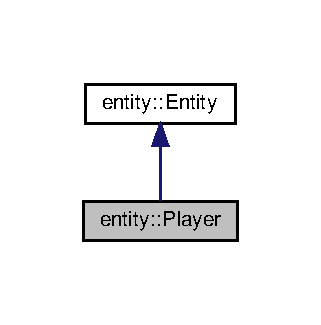
\includegraphics[width=193pt]{classentity_1_1Player__inherit__graph}
\end{center}
\end{figure}


Klasni dijagram za entity\+:\+:Player\+:
\nopagebreak
\begin{figure}[H]
\begin{center}
\leavevmode
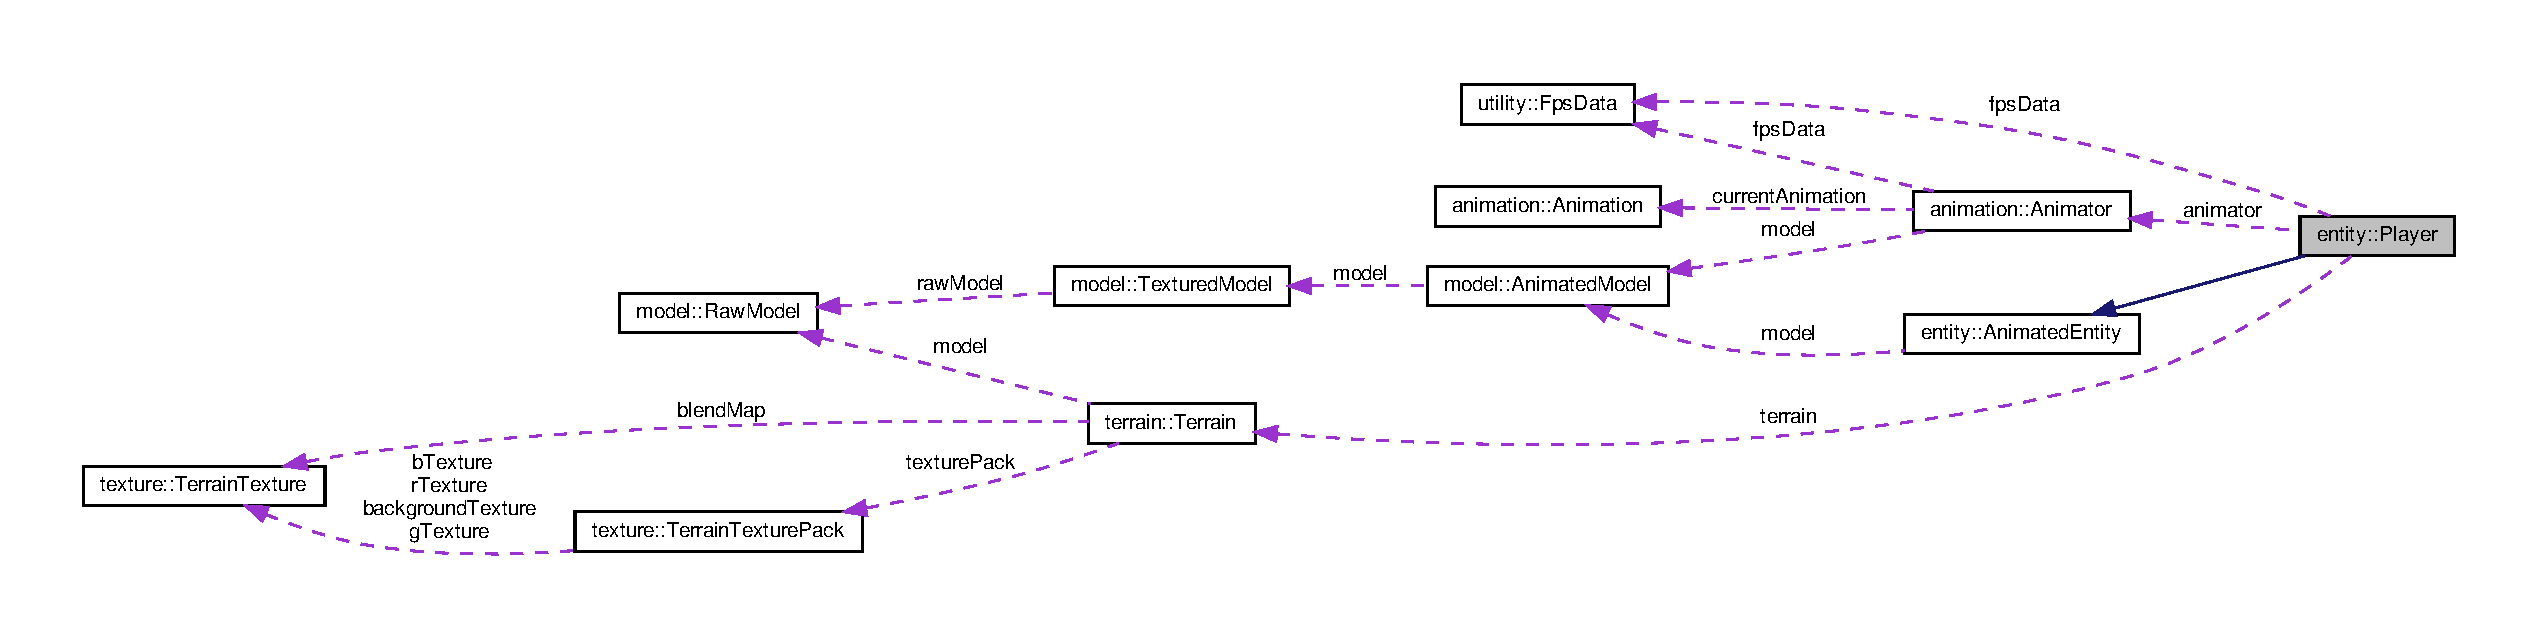
\includegraphics[width=350pt]{classentity_1_1Player__coll__graph}
\end{center}
\end{figure}
\subsection*{Javni članovi}
\begin{DoxyCompactItemize}
\item 
\hyperlink{classentity_1_1Player_ab96231144acc882d898ec60abd7ed702}{Player} (\hyperlink{classmodel_1_1AnimatedModel}{Animated\+Model} $\ast$\hyperlink{classentity_1_1AnimatedEntity_a1f9e73e14bf1588ed9e7c9e7f7d4aab3}{model}, vec3 \hyperlink{classentity_1_1AnimatedEntity_ab02891959f4c1191807e267c48466230}{position}, vec3 \hyperlink{classentity_1_1AnimatedEntity_a32f7718856950b74d40f4a96c1aa6f3d}{rotation}, float \hyperlink{classentity_1_1AnimatedEntity_a137e8fe0398142e9dedebb3eb1fe4f2f}{scale}, \hyperlink{classterrain_1_1Terrain}{Terrain} $\ast$\hyperlink{classentity_1_1Player_adc298ca7a3d8ab3528440489ed4ea60e}{terrain}, \hyperlink{classutility_1_1FpsData}{Fps\+Data} $\ast$\hyperlink{classentity_1_1Player_a830db86853301f3619dd4416c52229e4}{fps\+Data}, \hyperlink{classanimation_1_1Animator}{Animator} $\ast$\hyperlink{classentity_1_1Player_a77d9fff91395b091561f81b9acd5f034}{animator})
\begin{DoxyCompactList}\small\item\em Konstruktor klase. \end{DoxyCompactList}\item 
\hyperlink{classentity_1_1Player_aba0d4255d0d8624d01067418279bc9a1}{$\sim$\+Player} ()
\begin{DoxyCompactList}\small\item\em Destruktor klase. \end{DoxyCompactList}\item 
void \hyperlink{classentity_1_1Player_a27a2007873610439598c0ac07a91f3ac}{handle\+Key\+Up} (unsigned char key)
\begin{DoxyCompactList}\small\item\em Funkcija obradjuje ulaz sa tastature. \end{DoxyCompactList}\item 
void \hyperlink{classentity_1_1Player_af3d0b548d6daeb37d03f9fa57fb28f8a}{handle\+Key\+Down} (unsigned char key)
\begin{DoxyCompactList}\small\item\em Funkcija obradjuje ulaz sa tastature. \end{DoxyCompactList}\item 
void \hyperlink{classentity_1_1Player_a9b0a7ab96a4ba7c24c7ddac8f07c4d5e}{move} ()
\begin{DoxyCompactList}\small\item\em Funkcija pomera igraca. \end{DoxyCompactList}\end{DoxyCompactItemize}
\subsection*{Privatni članovi}
\begin{DoxyCompactItemize}
\item 
float \hyperlink{classentity_1_1Player_a06f0a95dc0b0efc3299a07f90e91dd25}{current\+Speed}
\begin{DoxyCompactList}\small\item\em Trenutna brzina igraca. \end{DoxyCompactList}\item 
float \hyperlink{classentity_1_1Player_afaac869e93409af86a6f6fc53a95687e}{current\+Turn\+Speed}
\begin{DoxyCompactList}\small\item\em Trenutna rotaciona brzina igraca. \end{DoxyCompactList}\item 
\hyperlink{classterrain_1_1Terrain}{Terrain} $\ast$ \hyperlink{classentity_1_1Player_adc298ca7a3d8ab3528440489ed4ea60e}{terrain}
\begin{DoxyCompactList}\small\item\em Pokazivac na instancu klase Terrain. \end{DoxyCompactList}\item 
bool $\ast$ \hyperlink{classentity_1_1Player_ad36623cb0c52ae4dc97d73cbf1cd2134}{key\+Buffer}
\begin{DoxyCompactList}\small\item\em Niz karaktera koji su pritisnuti a nisu otpusteni. \end{DoxyCompactList}\item 
\hyperlink{classutility_1_1FpsData}{Fps\+Data} $\ast$ \hyperlink{classentity_1_1Player_a830db86853301f3619dd4416c52229e4}{fps\+Data}
\begin{DoxyCompactList}\small\item\em Pokazivac na instancu klase Fps\+Data. \end{DoxyCompactList}\item 
\hyperlink{classanimation_1_1Animator}{Animator} $\ast$ \hyperlink{classentity_1_1Player_a77d9fff91395b091561f81b9acd5f034}{animator}
\begin{DoxyCompactList}\small\item\em Pokazivac na instancu klase Animator. \end{DoxyCompactList}\item 
bool \hyperlink{classentity_1_1Player_a92fb9b7321096cd6dedbcc31b12cf011}{animation\+On}
\begin{DoxyCompactList}\small\item\em Istinitosna vrednost koja oznacava da li je animacija aktivna. \end{DoxyCompactList}\end{DoxyCompactItemize}


\subsection{Opširniji opis}
Klasa \hyperlink{classentity_1_1Player}{Player} odredjuje igraca koji nadogradjuje entitet. Pomocu klase \hyperlink{classentity_1_1Player}{Player} nadogradjujemo klasu \hyperlink{classentity_1_1Entity}{Entity} dodavajuci jos nove atribute i funkcije. 

\subsection{Dokumentacija konstruktora i destruktora}
\mbox{\Hypertarget{classentity_1_1Player_ab96231144acc882d898ec60abd7ed702}\label{classentity_1_1Player_ab96231144acc882d898ec60abd7ed702}} 
\index{entity\+::\+Player@{entity\+::\+Player}!Player@{Player}}
\index{Player@{Player}!entity\+::\+Player@{entity\+::\+Player}}
\subsubsection{\texorpdfstring{Player()}{Player()}}
{\footnotesize\ttfamily entity\+::\+Player\+::\+Player (\begin{DoxyParamCaption}\item[{\hyperlink{classmodel_1_1AnimatedModel}{Animated\+Model} $\ast$}]{model,  }\item[{vec3}]{position,  }\item[{vec3}]{rotation,  }\item[{float}]{scale,  }\item[{\hyperlink{classterrain_1_1Terrain}{Terrain} $\ast$}]{terrain,  }\item[{\hyperlink{classutility_1_1FpsData}{Fps\+Data} $\ast$}]{fps\+Data,  }\item[{\hyperlink{classanimation_1_1Animator}{Animator} $\ast$}]{animator }\end{DoxyParamCaption})}



Konstruktor klase. 


\begin{DoxyParams}{Parametri}
{\em model} & Pokazivac na instancu klase Animated\+Model. \\
\hline
{\em position} & Pozicija entiteta. \\
\hline
{\em rotation} & Rotacija entiteta. \\
\hline
{\em scale} & Skaliranje entiteta. \\
\hline
{\em terrain} & Pokazivac na instancu klase Terrain. \\
\hline
{\em fps\+Data} & Pokazivac na instancu klase Fps\+Data. \\
\hline
{\em animator} & Pokazivac na instancu klase Animator. \\
\hline
\end{DoxyParams}
\mbox{\Hypertarget{classentity_1_1Player_aba0d4255d0d8624d01067418279bc9a1}\label{classentity_1_1Player_aba0d4255d0d8624d01067418279bc9a1}} 
\index{entity\+::\+Player@{entity\+::\+Player}!````~Player@{$\sim$\+Player}}
\index{````~Player@{$\sim$\+Player}!entity\+::\+Player@{entity\+::\+Player}}
\subsubsection{\texorpdfstring{$\sim$\+Player()}{~Player()}}
{\footnotesize\ttfamily entity\+::\+Player\+::$\sim$\+Player (\begin{DoxyParamCaption}{ }\end{DoxyParamCaption})}



Destruktor klase. 


\begin{DoxyParams}{Parametri}
{\em void} & \\
\hline
\end{DoxyParams}


\subsection{Dokumentacija funkcija članica}
\mbox{\Hypertarget{classentity_1_1Player_af3d0b548d6daeb37d03f9fa57fb28f8a}\label{classentity_1_1Player_af3d0b548d6daeb37d03f9fa57fb28f8a}} 
\index{entity\+::\+Player@{entity\+::\+Player}!handle\+Key\+Down@{handle\+Key\+Down}}
\index{handle\+Key\+Down@{handle\+Key\+Down}!entity\+::\+Player@{entity\+::\+Player}}
\subsubsection{\texorpdfstring{handle\+Key\+Down()}{handleKeyDown()}}
{\footnotesize\ttfamily void entity\+::\+Player\+::handle\+Key\+Down (\begin{DoxyParamCaption}\item[{unsigned char}]{key }\end{DoxyParamCaption})}



Funkcija obradjuje ulaz sa tastature. 


\begin{DoxyParams}{Parametri}
{\em key} & Karakter koji je pritisnut na tastaturi. \\
\hline
\end{DoxyParams}
\begin{DoxyReturn}{Vrednost funkcije}
void 
\end{DoxyReturn}
\mbox{\Hypertarget{classentity_1_1Player_a27a2007873610439598c0ac07a91f3ac}\label{classentity_1_1Player_a27a2007873610439598c0ac07a91f3ac}} 
\index{entity\+::\+Player@{entity\+::\+Player}!handle\+Key\+Up@{handle\+Key\+Up}}
\index{handle\+Key\+Up@{handle\+Key\+Up}!entity\+::\+Player@{entity\+::\+Player}}
\subsubsection{\texorpdfstring{handle\+Key\+Up()}{handleKeyUp()}}
{\footnotesize\ttfamily void entity\+::\+Player\+::handle\+Key\+Up (\begin{DoxyParamCaption}\item[{unsigned char}]{key }\end{DoxyParamCaption})}



Funkcija obradjuje ulaz sa tastature. 


\begin{DoxyParams}{Parametri}
{\em key} & Karakter koji je otpusten na tastaturi. \\
\hline
\end{DoxyParams}
\begin{DoxyReturn}{Vrednost funkcije}
void 
\end{DoxyReturn}
\mbox{\Hypertarget{classentity_1_1Player_a9b0a7ab96a4ba7c24c7ddac8f07c4d5e}\label{classentity_1_1Player_a9b0a7ab96a4ba7c24c7ddac8f07c4d5e}} 
\index{entity\+::\+Player@{entity\+::\+Player}!move@{move}}
\index{move@{move}!entity\+::\+Player@{entity\+::\+Player}}
\subsubsection{\texorpdfstring{move()}{move()}}
{\footnotesize\ttfamily void entity\+::\+Player\+::move (\begin{DoxyParamCaption}{ }\end{DoxyParamCaption})}



Funkcija pomera igraca. 


\begin{DoxyParams}{Parametri}
{\em void} & \\
\hline
\end{DoxyParams}
\begin{DoxyReturn}{Vrednost funkcije}
void 
\end{DoxyReturn}


\subsection{Dokumentacija atributa}
\mbox{\Hypertarget{classentity_1_1Player_a92fb9b7321096cd6dedbcc31b12cf011}\label{classentity_1_1Player_a92fb9b7321096cd6dedbcc31b12cf011}} 
\index{entity\+::\+Player@{entity\+::\+Player}!animation\+On@{animation\+On}}
\index{animation\+On@{animation\+On}!entity\+::\+Player@{entity\+::\+Player}}
\subsubsection{\texorpdfstring{animation\+On}{animationOn}}
{\footnotesize\ttfamily bool entity\+::\+Player\+::animation\+On\hspace{0.3cm}{\ttfamily [private]}}



Istinitosna vrednost koja oznacava da li je animacija aktivna. 

\mbox{\Hypertarget{classentity_1_1Player_a77d9fff91395b091561f81b9acd5f034}\label{classentity_1_1Player_a77d9fff91395b091561f81b9acd5f034}} 
\index{entity\+::\+Player@{entity\+::\+Player}!animator@{animator}}
\index{animator@{animator}!entity\+::\+Player@{entity\+::\+Player}}
\subsubsection{\texorpdfstring{animator}{animator}}
{\footnotesize\ttfamily \hyperlink{classanimation_1_1Animator}{Animator}$\ast$ entity\+::\+Player\+::animator\hspace{0.3cm}{\ttfamily [private]}}



Pokazivac na instancu klase Animator. 

\mbox{\Hypertarget{classentity_1_1Player_a06f0a95dc0b0efc3299a07f90e91dd25}\label{classentity_1_1Player_a06f0a95dc0b0efc3299a07f90e91dd25}} 
\index{entity\+::\+Player@{entity\+::\+Player}!current\+Speed@{current\+Speed}}
\index{current\+Speed@{current\+Speed}!entity\+::\+Player@{entity\+::\+Player}}
\subsubsection{\texorpdfstring{current\+Speed}{currentSpeed}}
{\footnotesize\ttfamily float entity\+::\+Player\+::current\+Speed\hspace{0.3cm}{\ttfamily [private]}}



Trenutna brzina igraca. 

\mbox{\Hypertarget{classentity_1_1Player_afaac869e93409af86a6f6fc53a95687e}\label{classentity_1_1Player_afaac869e93409af86a6f6fc53a95687e}} 
\index{entity\+::\+Player@{entity\+::\+Player}!current\+Turn\+Speed@{current\+Turn\+Speed}}
\index{current\+Turn\+Speed@{current\+Turn\+Speed}!entity\+::\+Player@{entity\+::\+Player}}
\subsubsection{\texorpdfstring{current\+Turn\+Speed}{currentTurnSpeed}}
{\footnotesize\ttfamily float entity\+::\+Player\+::current\+Turn\+Speed\hspace{0.3cm}{\ttfamily [private]}}



Trenutna rotaciona brzina igraca. 

\mbox{\Hypertarget{classentity_1_1Player_a830db86853301f3619dd4416c52229e4}\label{classentity_1_1Player_a830db86853301f3619dd4416c52229e4}} 
\index{entity\+::\+Player@{entity\+::\+Player}!fps\+Data@{fps\+Data}}
\index{fps\+Data@{fps\+Data}!entity\+::\+Player@{entity\+::\+Player}}
\subsubsection{\texorpdfstring{fps\+Data}{fpsData}}
{\footnotesize\ttfamily \hyperlink{classutility_1_1FpsData}{Fps\+Data}$\ast$ entity\+::\+Player\+::fps\+Data\hspace{0.3cm}{\ttfamily [private]}}



Pokazivac na instancu klase Fps\+Data. 

\mbox{\Hypertarget{classentity_1_1Player_ad36623cb0c52ae4dc97d73cbf1cd2134}\label{classentity_1_1Player_ad36623cb0c52ae4dc97d73cbf1cd2134}} 
\index{entity\+::\+Player@{entity\+::\+Player}!key\+Buffer@{key\+Buffer}}
\index{key\+Buffer@{key\+Buffer}!entity\+::\+Player@{entity\+::\+Player}}
\subsubsection{\texorpdfstring{key\+Buffer}{keyBuffer}}
{\footnotesize\ttfamily bool$\ast$ entity\+::\+Player\+::key\+Buffer\hspace{0.3cm}{\ttfamily [private]}}



Niz karaktera koji su pritisnuti a nisu otpusteni. 

\mbox{\Hypertarget{classentity_1_1Player_adc298ca7a3d8ab3528440489ed4ea60e}\label{classentity_1_1Player_adc298ca7a3d8ab3528440489ed4ea60e}} 
\index{entity\+::\+Player@{entity\+::\+Player}!terrain@{terrain}}
\index{terrain@{terrain}!entity\+::\+Player@{entity\+::\+Player}}
\subsubsection{\texorpdfstring{terrain}{terrain}}
{\footnotesize\ttfamily \hyperlink{classterrain_1_1Terrain}{Terrain}$\ast$ entity\+::\+Player\+::terrain\hspace{0.3cm}{\ttfamily [private]}}



Pokazivac na instancu klase Terrain. 



Dokumentacija ove klase je napravljena na osnovu sledećih datoteka\+:\begin{DoxyCompactItemize}
\item 
/home/dusan/\+Documents/\+R\+G146-\/vitez-\/reda-\/zmaja/include/entity/\hyperlink{Player_8h}{Player.\+h}\item 
/home/dusan/\+Documents/\+R\+G146-\/vitez-\/reda-\/zmaja/src/entity/\hyperlink{Player_8cpp}{Player.\+cpp}\end{DoxyCompactItemize}

\hypertarget{classmodel_1_1RawModel}{}\section{Dokumentacija klase model\+:\+:Raw\+Model}
\label{classmodel_1_1RawModel}\index{model\+::\+Raw\+Model@{model\+::\+Raw\+Model}}


Klasa \hyperlink{classmodel_1_1RawModel}{Raw\+Model} opisuje model objekta. Model je opisan brojem tacaka i pridruzenom nizu atributa.  




{\ttfamily \#include $<$Raw\+Model.\+h$>$}

\subsection*{Javni članovi}
\begin{DoxyCompactItemize}
\item 
\hyperlink{classmodel_1_1RawModel_ab1f77c2fa73575a79b65bae30cec98a6}{Raw\+Model} (vector$<$ G\+Lint $>$ \hyperlink{classmodel_1_1RawModel_a994176411e71716620d422dd56febbac}{meshes\+Vao\+ID}, vector$<$ G\+Lint $>$ \hyperlink{classmodel_1_1RawModel_a9a6ad9eb37bd6453ec115c2195d7f8a2}{meshes\+Vertex\+Count})
\begin{DoxyCompactList}\small\item\em Konstruktor klase. U konstruktoru se modelu pridruzuju broj tacaka objekta i identifikator niza atributa. \end{DoxyCompactList}\item 
\hyperlink{classmodel_1_1RawModel_a44e687484478b0747abe25baa3533b71}{$\sim$\+Raw\+Model} ()
\begin{DoxyCompactList}\small\item\em Destruktor klase. \end{DoxyCompactList}\item 
vector$<$ G\+Lint $>$ \hyperlink{classmodel_1_1RawModel_af13c9200466649ab5900eaeeeeefdbc4}{get\+Meshes\+Vao\+ID} (void)
\begin{DoxyCompactList}\small\item\em Funkcija vraca listu identifikatora niza atributa objekta. \end{DoxyCompactList}\item 
vector$<$ G\+Lint $>$ \hyperlink{classmodel_1_1RawModel_aafc5e5b7da34dda1c80cff89a65d08e5}{get\+Meshes\+Vertex\+Count} (void)
\begin{DoxyCompactList}\small\item\em Funkcija vraca listu broja tacaka objekta. \end{DoxyCompactList}\end{DoxyCompactItemize}
\subsection*{Privatni članovi}
\begin{DoxyCompactItemize}
\item 
vector$<$ G\+Lint $>$ \hyperlink{classmodel_1_1RawModel_a994176411e71716620d422dd56febbac}{meshes\+Vao\+ID}
\begin{DoxyCompactList}\small\item\em Identifikatori niza atributa. \end{DoxyCompactList}\item 
vector$<$ G\+Lint $>$ \hyperlink{classmodel_1_1RawModel_a9a6ad9eb37bd6453ec115c2195d7f8a2}{meshes\+Vertex\+Count}
\begin{DoxyCompactList}\small\item\em Broj tacaka objekta. \end{DoxyCompactList}\end{DoxyCompactItemize}


\subsection{Opširniji opis}
Klasa \hyperlink{classmodel_1_1RawModel}{Raw\+Model} opisuje model objekta. Model je opisan brojem tacaka i pridruzenom nizu atributa. 

\subsection{Dokumentacija konstruktora i destruktora}
\mbox{\Hypertarget{classmodel_1_1RawModel_ab1f77c2fa73575a79b65bae30cec98a6}\label{classmodel_1_1RawModel_ab1f77c2fa73575a79b65bae30cec98a6}} 
\index{model\+::\+Raw\+Model@{model\+::\+Raw\+Model}!Raw\+Model@{Raw\+Model}}
\index{Raw\+Model@{Raw\+Model}!model\+::\+Raw\+Model@{model\+::\+Raw\+Model}}
\subsubsection{\texorpdfstring{Raw\+Model()}{RawModel()}}
{\footnotesize\ttfamily model\+::\+Raw\+Model\+::\+Raw\+Model (\begin{DoxyParamCaption}\item[{vector$<$ G\+Lint $>$}]{meshes\+Vao\+ID,  }\item[{vector$<$ G\+Lint $>$}]{meshes\+Vertex\+Count }\end{DoxyParamCaption})}



Konstruktor klase. U konstruktoru se modelu pridruzuju broj tacaka objekta i identifikator niza atributa. 


\begin{DoxyParams}{Parametri}
{\em meshes\+Vao\+ID} & Lista identifikatora niza atributa. \\
\hline
{\em meshes\+Vertex\+Count} & Lista broja tacaka objekta. \\
\hline
\end{DoxyParams}
\mbox{\Hypertarget{classmodel_1_1RawModel_a44e687484478b0747abe25baa3533b71}\label{classmodel_1_1RawModel_a44e687484478b0747abe25baa3533b71}} 
\index{model\+::\+Raw\+Model@{model\+::\+Raw\+Model}!````~Raw\+Model@{$\sim$\+Raw\+Model}}
\index{````~Raw\+Model@{$\sim$\+Raw\+Model}!model\+::\+Raw\+Model@{model\+::\+Raw\+Model}}
\subsubsection{\texorpdfstring{$\sim$\+Raw\+Model()}{~RawModel()}}
{\footnotesize\ttfamily model\+::\+Raw\+Model\+::$\sim$\+Raw\+Model (\begin{DoxyParamCaption}{ }\end{DoxyParamCaption})}



Destruktor klase. 


\begin{DoxyParams}{Parametri}
{\em void} & \\
\hline
\end{DoxyParams}


\subsection{Dokumentacija funkcija članica}
\mbox{\Hypertarget{classmodel_1_1RawModel_af13c9200466649ab5900eaeeeeefdbc4}\label{classmodel_1_1RawModel_af13c9200466649ab5900eaeeeeefdbc4}} 
\index{model\+::\+Raw\+Model@{model\+::\+Raw\+Model}!get\+Meshes\+Vao\+ID@{get\+Meshes\+Vao\+ID}}
\index{get\+Meshes\+Vao\+ID@{get\+Meshes\+Vao\+ID}!model\+::\+Raw\+Model@{model\+::\+Raw\+Model}}
\subsubsection{\texorpdfstring{get\+Meshes\+Vao\+I\+D()}{getMeshesVaoID()}}
{\footnotesize\ttfamily vector$<$ G\+Lint $>$ model\+::\+Raw\+Model\+::get\+Meshes\+Vao\+ID (\begin{DoxyParamCaption}\item[{void}]{ }\end{DoxyParamCaption})}



Funkcija vraca listu identifikatora niza atributa objekta. 


\begin{DoxyParams}{Parametri}
{\em void} & \\
\hline
\end{DoxyParams}
\begin{DoxyReturn}{Vrednost funkcije}
vector$<$\+G\+Lint$>$ Lista identifikatora niza atributa. 
\end{DoxyReturn}
\mbox{\Hypertarget{classmodel_1_1RawModel_aafc5e5b7da34dda1c80cff89a65d08e5}\label{classmodel_1_1RawModel_aafc5e5b7da34dda1c80cff89a65d08e5}} 
\index{model\+::\+Raw\+Model@{model\+::\+Raw\+Model}!get\+Meshes\+Vertex\+Count@{get\+Meshes\+Vertex\+Count}}
\index{get\+Meshes\+Vertex\+Count@{get\+Meshes\+Vertex\+Count}!model\+::\+Raw\+Model@{model\+::\+Raw\+Model}}
\subsubsection{\texorpdfstring{get\+Meshes\+Vertex\+Count()}{getMeshesVertexCount()}}
{\footnotesize\ttfamily vector$<$ G\+Lint $>$ model\+::\+Raw\+Model\+::get\+Meshes\+Vertex\+Count (\begin{DoxyParamCaption}\item[{void}]{ }\end{DoxyParamCaption})}



Funkcija vraca listu broja tacaka objekta. 


\begin{DoxyParams}{Parametri}
{\em void} & \\
\hline
\end{DoxyParams}
\begin{DoxyReturn}{Vrednost funkcije}
vector$<$\+G\+Lint$>$ Lista broja tacaka objekta. 
\end{DoxyReturn}


\subsection{Dokumentacija atributa}
\mbox{\Hypertarget{classmodel_1_1RawModel_a994176411e71716620d422dd56febbac}\label{classmodel_1_1RawModel_a994176411e71716620d422dd56febbac}} 
\index{model\+::\+Raw\+Model@{model\+::\+Raw\+Model}!meshes\+Vao\+ID@{meshes\+Vao\+ID}}
\index{meshes\+Vao\+ID@{meshes\+Vao\+ID}!model\+::\+Raw\+Model@{model\+::\+Raw\+Model}}
\subsubsection{\texorpdfstring{meshes\+Vao\+ID}{meshesVaoID}}
{\footnotesize\ttfamily vector$<$G\+Lint$>$ model\+::\+Raw\+Model\+::meshes\+Vao\+ID\hspace{0.3cm}{\ttfamily [private]}}



Identifikatori niza atributa. 

\mbox{\Hypertarget{classmodel_1_1RawModel_a9a6ad9eb37bd6453ec115c2195d7f8a2}\label{classmodel_1_1RawModel_a9a6ad9eb37bd6453ec115c2195d7f8a2}} 
\index{model\+::\+Raw\+Model@{model\+::\+Raw\+Model}!meshes\+Vertex\+Count@{meshes\+Vertex\+Count}}
\index{meshes\+Vertex\+Count@{meshes\+Vertex\+Count}!model\+::\+Raw\+Model@{model\+::\+Raw\+Model}}
\subsubsection{\texorpdfstring{meshes\+Vertex\+Count}{meshesVertexCount}}
{\footnotesize\ttfamily vector$<$G\+Lint$>$ model\+::\+Raw\+Model\+::meshes\+Vertex\+Count\hspace{0.3cm}{\ttfamily [private]}}



Broj tacaka objekta. 



Dokumentacija ove klase je napravljena na osnovu sledećih datoteka\+:\begin{DoxyCompactItemize}
\item 
/home/dusan/\+Documents/\+R\+G146-\/vitez-\/reda-\/zmaja/include/model/\hyperlink{RawModel_8h}{Raw\+Model.\+h}\item 
/home/dusan/\+Documents/\+R\+G146-\/vitez-\/reda-\/zmaja/src/model/\hyperlink{RawModel_8cpp}{Raw\+Model.\+cpp}\end{DoxyCompactItemize}

\hypertarget{classcore_1_1Render}{}\section{Dokumentacija klase core\+:\+:Render}
\label{classcore_1_1Render}\index{core\+::\+Render@{core\+::\+Render}}


Klasa \hyperlink{classcore_1_1Render}{Render} je zaduzena za iscrtavanje entiteta na ekran. Tokom pokretanja prvo se vrsi priprema za iscrtavanje, a zatim se sadrzaj niza atributa(koordinate, boje, texture ...) iscrtava na ekran.  




{\ttfamily \#include $<$Render.\+h$>$}



Klasni dijagram za core\+:\+:Render\+:\nopagebreak
\begin{figure}[H]
\begin{center}
\leavevmode
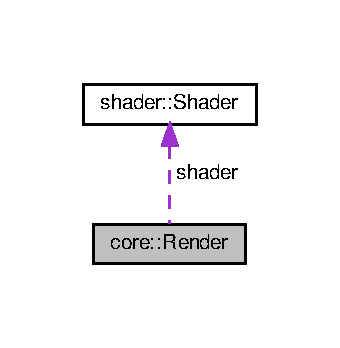
\includegraphics[width=163pt]{classcore_1_1Render__coll__graph}
\end{center}
\end{figure}
\subsection*{Javni članovi}
\begin{DoxyCompactItemize}
\item 
\hyperlink{classcore_1_1Render_ab101784fcf9fdb1f8f86b026fd47c2f6}{Render} (\hyperlink{classshader_1_1Shader}{Shader} $\ast$\hyperlink{classcore_1_1Render_a220be4bb26b6cbec909953f247a7732c}{shader})
\begin{DoxyCompactList}\small\item\em Konstruktor klase. \end{DoxyCompactList}\item 
\hyperlink{classcore_1_1Render_ac11786f4406333b24a33b61c5e2506f4}{$\sim$\+Render} ()
\begin{DoxyCompactList}\small\item\em Destruktor klase. \end{DoxyCompactList}\item 
void \hyperlink{classcore_1_1Render_ab36887be4cb2f56e73b10f78e5d04d4a}{render} (map$<$ \hyperlink{classmodel_1_1TexturedModel}{Textured\+Model} $\ast$, list$<$ \hyperlink{classentity_1_1Entity}{Entity} $\ast$$>$$>$ entities)
\begin{DoxyCompactList}\small\item\em Funkcija iscrtava sve entitete i teksturisane modele koje im odgovaraju. \end{DoxyCompactList}\item 
void \hyperlink{classcore_1_1Render_add7058167c0780784695497286c5e382}{prepare\+Textured\+Model} (\hyperlink{classmodel_1_1TexturedModel}{Textured\+Model} $\ast$\hyperlink{namespacecore_aa1479d4ed4dadbfe085b26662122b68a}{model})
\begin{DoxyCompactList}\small\item\em Funkcija ucitava teksture entiteta. \end{DoxyCompactList}\item 
void \hyperlink{classcore_1_1Render_adfa16af79f2e428b94ccbb406e77ef93}{unbind\+Textured\+Model} ()
\begin{DoxyCompactList}\small\item\em Funkcija otkacinje vezu izmedju podataka texturisanog modela i programa. \end{DoxyCompactList}\item 
void \hyperlink{classcore_1_1Render_aeb298077579c71d8b4407dacbed75302}{prepare\+Instance} (\hyperlink{classentity_1_1Entity}{Entity} $\ast$\hyperlink{namespacecore_aa710c0ea388433d2d80d1d1c67582eda}{entity})
\begin{DoxyCompactList}\small\item\em Funkcija kreira matricu transformacije za entitet i ucitava je u sejder program. \end{DoxyCompactList}\end{DoxyCompactItemize}
\subsection*{Privatni članovi}
\begin{DoxyCompactItemize}
\item 
mat4 \hyperlink{classcore_1_1Render_af0c1d960dc3ca1bab8abc1302d04c254}{create\+Projection\+Matrix} ()
\begin{DoxyCompactList}\small\item\em Funkcija kreira matricu projekcije. \end{DoxyCompactList}\end{DoxyCompactItemize}
\subsection*{Privatni članovi}
\begin{DoxyCompactItemize}
\item 
float \hyperlink{classcore_1_1Render_aab61f8ad63c67621572d45c3debfaff2}{F\+OV} = 70
\begin{DoxyCompactList}\small\item\em Polje vidika. \end{DoxyCompactList}\item 
float \hyperlink{classcore_1_1Render_a21b18ddc1ea04e877e9218e92cbb8a0a}{N\+E\+A\+R\+\_\+\+P\+L\+A\+NE} = 0.\+1
\begin{DoxyCompactList}\small\item\em Prednji deo vidljivosti. \end{DoxyCompactList}\item 
float \hyperlink{classcore_1_1Render_a331f4b9d510f06bbbbf85f06ac8995a2}{F\+A\+R\+\_\+\+P\+L\+A\+NE} = 1000
\begin{DoxyCompactList}\small\item\em Zadnji deo vidljivosti. \end{DoxyCompactList}\item 
\hyperlink{classshader_1_1Shader}{Shader} $\ast$ \hyperlink{classcore_1_1Render_a220be4bb26b6cbec909953f247a7732c}{shader}
\begin{DoxyCompactList}\small\item\em Pokazivac na instancu klase Shader. \end{DoxyCompactList}\end{DoxyCompactItemize}


\subsection{Opširniji opis}
Klasa \hyperlink{classcore_1_1Render}{Render} je zaduzena za iscrtavanje entiteta na ekran. Tokom pokretanja prvo se vrsi priprema za iscrtavanje, a zatim se sadrzaj niza atributa(koordinate, boje, texture ...) iscrtava na ekran. 

\subsection{Dokumentacija konstruktora i destruktora}
\mbox{\Hypertarget{classcore_1_1Render_ab101784fcf9fdb1f8f86b026fd47c2f6}\label{classcore_1_1Render_ab101784fcf9fdb1f8f86b026fd47c2f6}} 
\index{core\+::\+Render@{core\+::\+Render}!Render@{Render}}
\index{Render@{Render}!core\+::\+Render@{core\+::\+Render}}
\subsubsection{\texorpdfstring{Render()}{Render()}}
{\footnotesize\ttfamily core\+::\+Render\+::\+Render (\begin{DoxyParamCaption}\item[{\hyperlink{classshader_1_1Shader}{Shader} $\ast$}]{shader }\end{DoxyParamCaption})}



Konstruktor klase. 


\begin{DoxyParams}{Parametri}
{\em shader} & Pokazivac na instancu klase Shader. \\
\hline
\end{DoxyParams}
\mbox{\Hypertarget{classcore_1_1Render_ac11786f4406333b24a33b61c5e2506f4}\label{classcore_1_1Render_ac11786f4406333b24a33b61c5e2506f4}} 
\index{core\+::\+Render@{core\+::\+Render}!````~Render@{$\sim$\+Render}}
\index{````~Render@{$\sim$\+Render}!core\+::\+Render@{core\+::\+Render}}
\subsubsection{\texorpdfstring{$\sim$\+Render()}{~Render()}}
{\footnotesize\ttfamily core\+::\+Render\+::$\sim$\+Render (\begin{DoxyParamCaption}{ }\end{DoxyParamCaption})}



Destruktor klase. 


\begin{DoxyParams}{Parametri}
{\em void} & \\
\hline
\end{DoxyParams}


\subsection{Dokumentacija funkcija članica}
\mbox{\Hypertarget{classcore_1_1Render_af0c1d960dc3ca1bab8abc1302d04c254}\label{classcore_1_1Render_af0c1d960dc3ca1bab8abc1302d04c254}} 
\index{core\+::\+Render@{core\+::\+Render}!create\+Projection\+Matrix@{create\+Projection\+Matrix}}
\index{create\+Projection\+Matrix@{create\+Projection\+Matrix}!core\+::\+Render@{core\+::\+Render}}
\subsubsection{\texorpdfstring{create\+Projection\+Matrix()}{createProjectionMatrix()}}
{\footnotesize\ttfamily mat4 core\+::\+Render\+::create\+Projection\+Matrix (\begin{DoxyParamCaption}{ }\end{DoxyParamCaption})\hspace{0.3cm}{\ttfamily [private]}}



Funkcija kreira matricu projekcije. 


\begin{DoxyParams}{Parametri}
{\em void} & \\
\hline
\end{DoxyParams}
\begin{DoxyReturn}{Vrednost funkcije}
mat4 Matrica projekcije. 
\end{DoxyReturn}
\mbox{\Hypertarget{classcore_1_1Render_aeb298077579c71d8b4407dacbed75302}\label{classcore_1_1Render_aeb298077579c71d8b4407dacbed75302}} 
\index{core\+::\+Render@{core\+::\+Render}!prepare\+Instance@{prepare\+Instance}}
\index{prepare\+Instance@{prepare\+Instance}!core\+::\+Render@{core\+::\+Render}}
\subsubsection{\texorpdfstring{prepare\+Instance()}{prepareInstance()}}
{\footnotesize\ttfamily void core\+::\+Render\+::prepare\+Instance (\begin{DoxyParamCaption}\item[{\hyperlink{classentity_1_1Entity}{Entity} $\ast$}]{entity }\end{DoxyParamCaption})}



Funkcija kreira matricu transformacije za entitet i ucitava je u sejder program. 


\begin{DoxyParams}{Parametri}
{\em entity} & Pokazivac na instancu klase Entity. \\
\hline
\end{DoxyParams}
\begin{DoxyReturn}{Vrednost funkcije}
void 
\end{DoxyReturn}
\mbox{\Hypertarget{classcore_1_1Render_add7058167c0780784695497286c5e382}\label{classcore_1_1Render_add7058167c0780784695497286c5e382}} 
\index{core\+::\+Render@{core\+::\+Render}!prepare\+Textured\+Model@{prepare\+Textured\+Model}}
\index{prepare\+Textured\+Model@{prepare\+Textured\+Model}!core\+::\+Render@{core\+::\+Render}}
\subsubsection{\texorpdfstring{prepare\+Textured\+Model()}{prepareTexturedModel()}}
{\footnotesize\ttfamily void core\+::\+Render\+::prepare\+Textured\+Model (\begin{DoxyParamCaption}\item[{\hyperlink{classmodel_1_1TexturedModel}{Textured\+Model} $\ast$}]{model }\end{DoxyParamCaption})}



Funkcija ucitava teksture entiteta. 


\begin{DoxyParams}{Parametri}
{\em model} & Pokazivac na instancu klase Textured\+Model. \\
\hline
\end{DoxyParams}
\begin{DoxyReturn}{Vrednost funkcije}
void 
\end{DoxyReturn}
\mbox{\Hypertarget{classcore_1_1Render_ab36887be4cb2f56e73b10f78e5d04d4a}\label{classcore_1_1Render_ab36887be4cb2f56e73b10f78e5d04d4a}} 
\index{core\+::\+Render@{core\+::\+Render}!render@{render}}
\index{render@{render}!core\+::\+Render@{core\+::\+Render}}
\subsubsection{\texorpdfstring{render()}{render()}}
{\footnotesize\ttfamily void core\+::\+Render\+::render (\begin{DoxyParamCaption}\item[{map$<$ \hyperlink{classmodel_1_1TexturedModel}{Textured\+Model} $\ast$, list$<$ \hyperlink{classentity_1_1Entity}{Entity} $\ast$$>$$>$}]{entities }\end{DoxyParamCaption})}



Funkcija iscrtava sve entitete i teksturisane modele koje im odgovaraju. 


\begin{DoxyParams}{Parametri}
{\em entities} & Hes mapa teksturisanih modela i lista entiteta. \\
\hline
\end{DoxyParams}
\begin{DoxyReturn}{Vrednost funkcije}
void 
\end{DoxyReturn}
\mbox{\Hypertarget{classcore_1_1Render_adfa16af79f2e428b94ccbb406e77ef93}\label{classcore_1_1Render_adfa16af79f2e428b94ccbb406e77ef93}} 
\index{core\+::\+Render@{core\+::\+Render}!unbind\+Textured\+Model@{unbind\+Textured\+Model}}
\index{unbind\+Textured\+Model@{unbind\+Textured\+Model}!core\+::\+Render@{core\+::\+Render}}
\subsubsection{\texorpdfstring{unbind\+Textured\+Model()}{unbindTexturedModel()}}
{\footnotesize\ttfamily void core\+::\+Render\+::unbind\+Textured\+Model (\begin{DoxyParamCaption}{ }\end{DoxyParamCaption})}



Funkcija otkacinje vezu izmedju podataka texturisanog modela i programa. 


\begin{DoxyParams}{Parametri}
{\em void} & \\
\hline
\end{DoxyParams}
\begin{DoxyReturn}{Vrednost funkcije}
void 
\end{DoxyReturn}


\subsection{Dokumentacija atributa}
\mbox{\Hypertarget{classcore_1_1Render_a331f4b9d510f06bbbbf85f06ac8995a2}\label{classcore_1_1Render_a331f4b9d510f06bbbbf85f06ac8995a2}} 
\index{core\+::\+Render@{core\+::\+Render}!F\+A\+R\+\_\+\+P\+L\+A\+NE@{F\+A\+R\+\_\+\+P\+L\+A\+NE}}
\index{F\+A\+R\+\_\+\+P\+L\+A\+NE@{F\+A\+R\+\_\+\+P\+L\+A\+NE}!core\+::\+Render@{core\+::\+Render}}
\subsubsection{\texorpdfstring{F\+A\+R\+\_\+\+P\+L\+A\+NE}{FAR\_PLANE}}
{\footnotesize\ttfamily float core\+::\+Render\+::\+F\+A\+R\+\_\+\+P\+L\+A\+NE = 1000\hspace{0.3cm}{\ttfamily [private]}}



Zadnji deo vidljivosti. 

\mbox{\Hypertarget{classcore_1_1Render_aab61f8ad63c67621572d45c3debfaff2}\label{classcore_1_1Render_aab61f8ad63c67621572d45c3debfaff2}} 
\index{core\+::\+Render@{core\+::\+Render}!F\+OV@{F\+OV}}
\index{F\+OV@{F\+OV}!core\+::\+Render@{core\+::\+Render}}
\subsubsection{\texorpdfstring{F\+OV}{FOV}}
{\footnotesize\ttfamily float core\+::\+Render\+::\+F\+OV = 70\hspace{0.3cm}{\ttfamily [private]}}



Polje vidika. 

\mbox{\Hypertarget{classcore_1_1Render_a21b18ddc1ea04e877e9218e92cbb8a0a}\label{classcore_1_1Render_a21b18ddc1ea04e877e9218e92cbb8a0a}} 
\index{core\+::\+Render@{core\+::\+Render}!N\+E\+A\+R\+\_\+\+P\+L\+A\+NE@{N\+E\+A\+R\+\_\+\+P\+L\+A\+NE}}
\index{N\+E\+A\+R\+\_\+\+P\+L\+A\+NE@{N\+E\+A\+R\+\_\+\+P\+L\+A\+NE}!core\+::\+Render@{core\+::\+Render}}
\subsubsection{\texorpdfstring{N\+E\+A\+R\+\_\+\+P\+L\+A\+NE}{NEAR\_PLANE}}
{\footnotesize\ttfamily float core\+::\+Render\+::\+N\+E\+A\+R\+\_\+\+P\+L\+A\+NE = 0.\+1\hspace{0.3cm}{\ttfamily [private]}}



Prednji deo vidljivosti. 

\mbox{\Hypertarget{classcore_1_1Render_a220be4bb26b6cbec909953f247a7732c}\label{classcore_1_1Render_a220be4bb26b6cbec909953f247a7732c}} 
\index{core\+::\+Render@{core\+::\+Render}!shader@{shader}}
\index{shader@{shader}!core\+::\+Render@{core\+::\+Render}}
\subsubsection{\texorpdfstring{shader}{shader}}
{\footnotesize\ttfamily \hyperlink{classshader_1_1Shader}{Shader}$\ast$ core\+::\+Render\+::shader\hspace{0.3cm}{\ttfamily [private]}}



Pokazivac na instancu klase Shader. 



Dokumentacija ove klase je napravljena na osnovu sledećih datoteka\+:\begin{DoxyCompactItemize}
\item 
/home/dusan/\+Documents/\+R\+G146-\/vitez-\/reda-\/zmaja/include/core/\hyperlink{Render_8h}{Render.\+h}\item 
/home/dusan/\+Documents/\+R\+G146-\/vitez-\/reda-\/zmaja/src/core/\hyperlink{Render_8cpp}{Render.\+cpp}\end{DoxyCompactItemize}

\hypertarget{classshader_1_1Shader}{}\section{Dokumentacija klase shader\+:\+:Shader}
\label{classshader_1_1Shader}\index{shader\+::\+Shader@{shader\+::\+Shader}}


Klasa \hyperlink{classshader_1_1Shader}{Shader} ucitava i izvrsava programe na Open\+GL Shading jeziku. Ucitavaju se sejder fajlovi koji se zatim kompajliraju i po potrebi se izvrsavaju i zaustavljaju.  




{\ttfamily \#include $<$Shader.\+h$>$}

\subsection*{Javni članovi}
\begin{DoxyCompactItemize}
\item 
\hyperlink{classshader_1_1Shader_a8346a24ed22edf1b1736cbe02dd27758}{Shader} (const char $\ast$vertex\+Shader\+File, const char $\ast$fragment\+Shader\+File)
\begin{DoxyCompactList}\small\item\em Konstruktor klase. U konstruktoru se ucitavaju sejder fajlovi i povezuju sa programom. \end{DoxyCompactList}\item 
\hyperlink{classshader_1_1Shader_a8d9b3ffe1ba804f91a26bd79a7588a34}{$\sim$\+Shader} ()
\begin{DoxyCompactList}\small\item\em Destruktor klase. \end{DoxyCompactList}\item 
void \hyperlink{classshader_1_1Shader_a879993e6f90506d6c9c0b9a39d1caebb}{bind\+Attribute} (int index, const char $\ast$variable\+Name)
\begin{DoxyCompactList}\small\item\em Funkcija povezuje ime sa generickim atributom. \end{DoxyCompactList}\item 
void \hyperlink{classshader_1_1Shader_a0b80abf1266063b5b2dea30422dd3358}{bind\+Attributes} (void)
\begin{DoxyCompactList}\small\item\em Funkcija povezuje sve potrebne atribute. \end{DoxyCompactList}\item 
void \hyperlink{classshader_1_1Shader_adb075db73fc6fc5e6bf4d924bc11e6c6}{start} (void)
\begin{DoxyCompactList}\small\item\em Funkcija pokrece sejder program. \end{DoxyCompactList}\item 
void \hyperlink{classshader_1_1Shader_a47fa58ad9ede974fe115c73c15c59691}{stop} (void)
\begin{DoxyCompactList}\small\item\em Funkcija zaustavlja sejder program. \end{DoxyCompactList}\item 
void \hyperlink{classshader_1_1Shader_af79c5615b39eae7e6368508429645c33}{clean\+Up} (void)
\begin{DoxyCompactList}\small\item\em Funkcija zaustavlja sejder program. \end{DoxyCompactList}\item 
int \hyperlink{classshader_1_1Shader_a91ddc84588431a520654096a74ca3671}{get\+Uniform\+Location} (const char $\ast$uniform\+Name)
\begin{DoxyCompactList}\small\item\em Funkcija vraca lokaciju uniformne promenljive. \end{DoxyCompactList}\item 
void \hyperlink{classshader_1_1Shader_a31d479c8502f9172c8b9393be362f391}{get\+All\+Uniform\+Locations} (void)
\begin{DoxyCompactList}\small\item\em Funkcija postavlja lokacije svih uniformnih promenljivih. \end{DoxyCompactList}\item 
void \hyperlink{classshader_1_1Shader_ae9dde8789a747d037f136c91a8cc03b6}{load\+Float} (int uniform\+Location, float value)
\begin{DoxyCompactList}\small\item\em Funkcija ucitava broj u uniformnu varijablu. \end{DoxyCompactList}\item 
void \hyperlink{classshader_1_1Shader_a06b6080ebb6c1735747771678dbec4b6}{load\+Float\+Vertex} (int uniform\+Location, vec3 vertex)
\begin{DoxyCompactList}\small\item\em Funkcija ucitava vektor koordinata u uniformnu varijablu. \end{DoxyCompactList}\item 
void \hyperlink{classshader_1_1Shader_acb1ec74c8d2ad5218669ece88a6dd491}{load\+Boolean} (int uniform\+Location, bool value)
\begin{DoxyCompactList}\small\item\em Funkcija ucitava istinitosnu vrednost u uniformnu varijablu. \end{DoxyCompactList}\item 
void \hyperlink{classshader_1_1Shader_ac2d90fdd4dfb7077046ec35b050660ee}{load\+Matrix} (int uniform\+Location, mat4 matrix)
\begin{DoxyCompactList}\small\item\em Funkcija ucitava matricu u uniformnu varijablu. \end{DoxyCompactList}\item 
void \hyperlink{classshader_1_1Shader_a5f73b4e8e0e9a72ea40072207394952d}{load\+Transformation\+Matrix} (mat4 matrix)
\begin{DoxyCompactList}\small\item\em Funkcija ucitava matricu transformacije u uniformnu varijablu. \end{DoxyCompactList}\item 
void \hyperlink{classshader_1_1Shader_a574d7ff5ab4870990795f72014e1aa1e}{load\+Projection\+Matrix} (mat4 matrix)
\begin{DoxyCompactList}\small\item\em Funkcija ucitava matricu projekcije u uniformnu varijablu. \end{DoxyCompactList}\item 
void \hyperlink{classshader_1_1Shader_ad7b79e54bfa3f757e3cf0104904e3dc3}{load\+View\+Matrix} (\hyperlink{classentity_1_1Camera}{Camera} $\ast$camera)
\begin{DoxyCompactList}\small\item\em Funkcija ucitava matricu pogleda u uniformnu varijablu. \end{DoxyCompactList}\item 
void \hyperlink{classshader_1_1Shader_abe287aa3d352de4e8aac6677666b90d1}{load\+Light} (\hyperlink{classentity_1_1Light}{Light} $\ast$light)
\begin{DoxyCompactList}\small\item\em Funkcija ucitava svetlost u uniformnu varijablu. \end{DoxyCompactList}\item 
void \hyperlink{classshader_1_1Shader_acd4755a3b83ebb6b0577832609cc520f}{load\+Shine\+Variables} (float shine, float reflectivity)
\begin{DoxyCompactList}\small\item\em Funkcija ucitava promenljive u uniformnu varijablu. \end{DoxyCompactList}\item 
void \hyperlink{classshader_1_1Shader_ace9f5d9ac79e04082aafa33c22d9f96c}{load\+Sky\+Colour} (float r, float g, float b)
\begin{DoxyCompactList}\small\item\em Funkcija ucitava boju neba u uniformnu varijablu. \end{DoxyCompactList}\item 
void \hyperlink{classshader_1_1Shader_a124ef086687ad7bcb0050c9fd1b13a24}{load\+Fake\+Lightning} (bool use\+Fake\+Lightning)
\begin{DoxyCompactList}\small\item\em Funkcija ucitava lazno osvetljenje u uniformnu varijablu. \end{DoxyCompactList}\end{DoxyCompactItemize}
\subsection*{Privatni članovi}
\begin{DoxyCompactItemize}
\item 
int \hyperlink{classshader_1_1Shader_aeabeeeb9e04b2704d6b22ff4a472afae}{load\+Shader} (const char $\ast$file\+Name, G\+Lenum type)
\begin{DoxyCompactList}\small\item\em Funkcija ucitava sejder fajlove. \end{DoxyCompactList}\end{DoxyCompactItemize}
\subsection*{Privatni članovi}
\begin{DoxyCompactItemize}
\item 
int \hyperlink{classshader_1_1Shader_a11598ec50991c2e59757634e5a38e02d}{program\+ID}
\begin{DoxyCompactList}\small\item\em Identifikator programa koji izvrsava sejder fajlove. \end{DoxyCompactList}\item 
int \hyperlink{classshader_1_1Shader_a6712aab22966fbf9db710aa53945c3c1}{vertex\+Shader\+ID}
\begin{DoxyCompactList}\small\item\em Identifikator ucitanog sejder fajla. \end{DoxyCompactList}\item 
int \hyperlink{classshader_1_1Shader_acbf60b0af53b36fdf5db868591579bf5}{fragment\+Shader\+ID}
\begin{DoxyCompactList}\small\item\em Identifikator ucitanog sejder fajla. \end{DoxyCompactList}\item 
int \hyperlink{classshader_1_1Shader_a7afd377d96d78de28c2acbda73b73e21}{location\+Transformation\+Matrix}
\begin{DoxyCompactList}\small\item\em Lokacija unformne promenljive. \end{DoxyCompactList}\item 
int \hyperlink{classshader_1_1Shader_aaa8ea0af1d2caf3f44ce08cfe26e1558}{location\+Projection\+Matrix}
\begin{DoxyCompactList}\small\item\em Lokacija unformne promenljive. \end{DoxyCompactList}\item 
int \hyperlink{classshader_1_1Shader_a59d584f36e417f8722b500522d9c41f0}{location\+View\+Matrix}
\begin{DoxyCompactList}\small\item\em Lokacija unformne promenljive. \end{DoxyCompactList}\item 
int \hyperlink{classshader_1_1Shader_a3f2c103127077c7a7a92260f6161055c}{location\+Light\+Position}
\begin{DoxyCompactList}\small\item\em Lokacija unformne promenljive. \end{DoxyCompactList}\item 
int \hyperlink{classshader_1_1Shader_a3aa71dac965d453a149b74e8282e6863}{location\+Light\+Colour}
\begin{DoxyCompactList}\small\item\em Lokacija unformne promenljive. \end{DoxyCompactList}\item 
int \hyperlink{classshader_1_1Shader_a7b1653ae0ccaa625e728ba76940d82f4}{location\+Shine}
\begin{DoxyCompactList}\small\item\em Lokacija unformne promenljive. \end{DoxyCompactList}\item 
int \hyperlink{classshader_1_1Shader_ad31f87938d470ce130a7053da45af551}{location\+Reflectivity}
\begin{DoxyCompactList}\small\item\em Lokacija unformne promenljive. \end{DoxyCompactList}\item 
int \hyperlink{classshader_1_1Shader_af74548a61cd3a07047dcf2d9adb5a9a9}{location\+Sky\+Colour}
\begin{DoxyCompactList}\small\item\em Lokacija unformne promenljive. \end{DoxyCompactList}\item 
int \hyperlink{classshader_1_1Shader_a07f4f399ad468c2c3af89e185d157813}{location\+Use\+Fake\+Lightning}
\begin{DoxyCompactList}\small\item\em Lokacija unformne promenljive. \end{DoxyCompactList}\end{DoxyCompactItemize}


\subsection{Opširniji opis}
Klasa \hyperlink{classshader_1_1Shader}{Shader} ucitava i izvrsava programe na Open\+GL Shading jeziku. Ucitavaju se sejder fajlovi koji se zatim kompajliraju i po potrebi se izvrsavaju i zaustavljaju. 

\subsection{Dokumentacija konstruktora i destruktora}
\mbox{\Hypertarget{classshader_1_1Shader_a8346a24ed22edf1b1736cbe02dd27758}\label{classshader_1_1Shader_a8346a24ed22edf1b1736cbe02dd27758}} 
\index{shader\+::\+Shader@{shader\+::\+Shader}!Shader@{Shader}}
\index{Shader@{Shader}!shader\+::\+Shader@{shader\+::\+Shader}}
\subsubsection{\texorpdfstring{Shader()}{Shader()}}
{\footnotesize\ttfamily shader\+::\+Shader\+::\+Shader (\begin{DoxyParamCaption}\item[{const char $\ast$}]{vertex\+Shader\+File,  }\item[{const char $\ast$}]{fragment\+Shader\+File }\end{DoxyParamCaption})}



Konstruktor klase. U konstruktoru se ucitavaju sejder fajlovi i povezuju sa programom. 


\begin{DoxyParams}{Parametri}
{\em vertex\+Shader\+File} & Ime sejder fajla. \\
\hline
{\em fragment\+Shader\+File} & Ime sejder fajla. \\
\hline
\end{DoxyParams}
\mbox{\Hypertarget{classshader_1_1Shader_a8d9b3ffe1ba804f91a26bd79a7588a34}\label{classshader_1_1Shader_a8d9b3ffe1ba804f91a26bd79a7588a34}} 
\index{shader\+::\+Shader@{shader\+::\+Shader}!````~Shader@{$\sim$\+Shader}}
\index{````~Shader@{$\sim$\+Shader}!shader\+::\+Shader@{shader\+::\+Shader}}
\subsubsection{\texorpdfstring{$\sim$\+Shader()}{~Shader()}}
{\footnotesize\ttfamily shader\+::\+Shader\+::$\sim$\+Shader (\begin{DoxyParamCaption}{ }\end{DoxyParamCaption})}



Destruktor klase. 


\begin{DoxyParams}{Parametri}
{\em void} & \\
\hline
\end{DoxyParams}


\subsection{Dokumentacija funkcija članica}
\mbox{\Hypertarget{classshader_1_1Shader_a879993e6f90506d6c9c0b9a39d1caebb}\label{classshader_1_1Shader_a879993e6f90506d6c9c0b9a39d1caebb}} 
\index{shader\+::\+Shader@{shader\+::\+Shader}!bind\+Attribute@{bind\+Attribute}}
\index{bind\+Attribute@{bind\+Attribute}!shader\+::\+Shader@{shader\+::\+Shader}}
\subsubsection{\texorpdfstring{bind\+Attribute()}{bindAttribute()}}
{\footnotesize\ttfamily void shader\+::\+Shader\+::bind\+Attribute (\begin{DoxyParamCaption}\item[{int}]{index,  }\item[{const char $\ast$}]{variable\+Name }\end{DoxyParamCaption})}



Funkcija povezuje ime sa generickim atributom. 


\begin{DoxyParams}{Parametri}
{\em index} & Identifikator generickog atributa \\
\hline
{\em variable\+Name} & Ime koje pridruzujemo generickom atributu \\
\hline
\end{DoxyParams}
\begin{DoxyReturn}{Vrednost funkcije}
void 
\end{DoxyReturn}
\mbox{\Hypertarget{classshader_1_1Shader_a0b80abf1266063b5b2dea30422dd3358}\label{classshader_1_1Shader_a0b80abf1266063b5b2dea30422dd3358}} 
\index{shader\+::\+Shader@{shader\+::\+Shader}!bind\+Attributes@{bind\+Attributes}}
\index{bind\+Attributes@{bind\+Attributes}!shader\+::\+Shader@{shader\+::\+Shader}}
\subsubsection{\texorpdfstring{bind\+Attributes()}{bindAttributes()}}
{\footnotesize\ttfamily void shader\+::\+Shader\+::bind\+Attributes (\begin{DoxyParamCaption}\item[{void}]{ }\end{DoxyParamCaption})}



Funkcija povezuje sve potrebne atribute. 


\begin{DoxyParams}{Parametri}
{\em void} & \\
\hline
\end{DoxyParams}
\begin{DoxyReturn}{Vrednost funkcije}
void 
\end{DoxyReturn}
\mbox{\Hypertarget{classshader_1_1Shader_af79c5615b39eae7e6368508429645c33}\label{classshader_1_1Shader_af79c5615b39eae7e6368508429645c33}} 
\index{shader\+::\+Shader@{shader\+::\+Shader}!clean\+Up@{clean\+Up}}
\index{clean\+Up@{clean\+Up}!shader\+::\+Shader@{shader\+::\+Shader}}
\subsubsection{\texorpdfstring{clean\+Up()}{cleanUp()}}
{\footnotesize\ttfamily void shader\+::\+Shader\+::clean\+Up (\begin{DoxyParamCaption}\item[{void}]{ }\end{DoxyParamCaption})}



Funkcija zaustavlja sejder program. 


\begin{DoxyParams}{Parametri}
{\em void} & \\
\hline
\end{DoxyParams}
\begin{DoxyReturn}{Vrednost funkcije}
void 
\end{DoxyReturn}
\mbox{\Hypertarget{classshader_1_1Shader_a31d479c8502f9172c8b9393be362f391}\label{classshader_1_1Shader_a31d479c8502f9172c8b9393be362f391}} 
\index{shader\+::\+Shader@{shader\+::\+Shader}!get\+All\+Uniform\+Locations@{get\+All\+Uniform\+Locations}}
\index{get\+All\+Uniform\+Locations@{get\+All\+Uniform\+Locations}!shader\+::\+Shader@{shader\+::\+Shader}}
\subsubsection{\texorpdfstring{get\+All\+Uniform\+Locations()}{getAllUniformLocations()}}
{\footnotesize\ttfamily void shader\+::\+Shader\+::get\+All\+Uniform\+Locations (\begin{DoxyParamCaption}\item[{void}]{ }\end{DoxyParamCaption})}



Funkcija postavlja lokacije svih uniformnih promenljivih. 


\begin{DoxyParams}{Parametri}
{\em void} & \\
\hline
\end{DoxyParams}
\begin{DoxyReturn}{Vrednost funkcije}
void 
\end{DoxyReturn}
\mbox{\Hypertarget{classshader_1_1Shader_a91ddc84588431a520654096a74ca3671}\label{classshader_1_1Shader_a91ddc84588431a520654096a74ca3671}} 
\index{shader\+::\+Shader@{shader\+::\+Shader}!get\+Uniform\+Location@{get\+Uniform\+Location}}
\index{get\+Uniform\+Location@{get\+Uniform\+Location}!shader\+::\+Shader@{shader\+::\+Shader}}
\subsubsection{\texorpdfstring{get\+Uniform\+Location()}{getUniformLocation()}}
{\footnotesize\ttfamily int shader\+::\+Shader\+::get\+Uniform\+Location (\begin{DoxyParamCaption}\item[{const char $\ast$}]{uniform\+Name }\end{DoxyParamCaption})}



Funkcija vraca lokaciju uniformne promenljive. 


\begin{DoxyParams}{Parametri}
{\em uniform\+Name} & Ime uniformne promenljive \\
\hline
\end{DoxyParams}
\begin{DoxyReturn}{Vrednost funkcije}
int Lokacija uniformne promenljive 
\end{DoxyReturn}
\mbox{\Hypertarget{classshader_1_1Shader_acb1ec74c8d2ad5218669ece88a6dd491}\label{classshader_1_1Shader_acb1ec74c8d2ad5218669ece88a6dd491}} 
\index{shader\+::\+Shader@{shader\+::\+Shader}!load\+Boolean@{load\+Boolean}}
\index{load\+Boolean@{load\+Boolean}!shader\+::\+Shader@{shader\+::\+Shader}}
\subsubsection{\texorpdfstring{load\+Boolean()}{loadBoolean()}}
{\footnotesize\ttfamily void shader\+::\+Shader\+::load\+Boolean (\begin{DoxyParamCaption}\item[{int}]{uniform\+Location,  }\item[{bool}]{value }\end{DoxyParamCaption})}



Funkcija ucitava istinitosnu vrednost u uniformnu varijablu. 


\begin{DoxyParams}{Parametri}
{\em uniform\+Location} & Lokacija uniformne promenljive \\
\hline
{\em value} & Istinitosna vrednost \\
\hline
\end{DoxyParams}
\begin{DoxyReturn}{Vrednost funkcije}
void 
\end{DoxyReturn}
\mbox{\Hypertarget{classshader_1_1Shader_a124ef086687ad7bcb0050c9fd1b13a24}\label{classshader_1_1Shader_a124ef086687ad7bcb0050c9fd1b13a24}} 
\index{shader\+::\+Shader@{shader\+::\+Shader}!load\+Fake\+Lightning@{load\+Fake\+Lightning}}
\index{load\+Fake\+Lightning@{load\+Fake\+Lightning}!shader\+::\+Shader@{shader\+::\+Shader}}
\subsubsection{\texorpdfstring{load\+Fake\+Lightning()}{loadFakeLightning()}}
{\footnotesize\ttfamily void shader\+::\+Shader\+::load\+Fake\+Lightning (\begin{DoxyParamCaption}\item[{bool}]{use\+Fake\+Lightning }\end{DoxyParamCaption})}



Funkcija ucitava lazno osvetljenje u uniformnu varijablu. 


\begin{DoxyParams}{Parametri}
{\em use\+Fake\+Lightning} & Istinitosna vrednost za koriscenje laznog osvetljenja \\
\hline
\end{DoxyParams}
\begin{DoxyReturn}{Vrednost funkcije}
void 
\end{DoxyReturn}
\mbox{\Hypertarget{classshader_1_1Shader_ae9dde8789a747d037f136c91a8cc03b6}\label{classshader_1_1Shader_ae9dde8789a747d037f136c91a8cc03b6}} 
\index{shader\+::\+Shader@{shader\+::\+Shader}!load\+Float@{load\+Float}}
\index{load\+Float@{load\+Float}!shader\+::\+Shader@{shader\+::\+Shader}}
\subsubsection{\texorpdfstring{load\+Float()}{loadFloat()}}
{\footnotesize\ttfamily void shader\+::\+Shader\+::load\+Float (\begin{DoxyParamCaption}\item[{int}]{uniform\+Location,  }\item[{float}]{value }\end{DoxyParamCaption})}



Funkcija ucitava broj u uniformnu varijablu. 


\begin{DoxyParams}{Parametri}
{\em uniform\+Location} & Lokacija uniformne promenljive \\
\hline
{\em value} & Broj pokretnom zarezu \\
\hline
\end{DoxyParams}
\begin{DoxyReturn}{Vrednost funkcije}
void 
\end{DoxyReturn}
\mbox{\Hypertarget{classshader_1_1Shader_a06b6080ebb6c1735747771678dbec4b6}\label{classshader_1_1Shader_a06b6080ebb6c1735747771678dbec4b6}} 
\index{shader\+::\+Shader@{shader\+::\+Shader}!load\+Float\+Vertex@{load\+Float\+Vertex}}
\index{load\+Float\+Vertex@{load\+Float\+Vertex}!shader\+::\+Shader@{shader\+::\+Shader}}
\subsubsection{\texorpdfstring{load\+Float\+Vertex()}{loadFloatVertex()}}
{\footnotesize\ttfamily void shader\+::\+Shader\+::load\+Float\+Vertex (\begin{DoxyParamCaption}\item[{int}]{uniform\+Location,  }\item[{vec3}]{vertex }\end{DoxyParamCaption})}



Funkcija ucitava vektor koordinata u uniformnu varijablu. 


\begin{DoxyParams}{Parametri}
{\em uniform\+Location} & Lokacija uniformne promenljive \\
\hline
{\em vertex} & Vektor koordinata \\
\hline
\end{DoxyParams}
\begin{DoxyReturn}{Vrednost funkcije}
void 
\end{DoxyReturn}
\mbox{\Hypertarget{classshader_1_1Shader_abe287aa3d352de4e8aac6677666b90d1}\label{classshader_1_1Shader_abe287aa3d352de4e8aac6677666b90d1}} 
\index{shader\+::\+Shader@{shader\+::\+Shader}!load\+Light@{load\+Light}}
\index{load\+Light@{load\+Light}!shader\+::\+Shader@{shader\+::\+Shader}}
\subsubsection{\texorpdfstring{load\+Light()}{loadLight()}}
{\footnotesize\ttfamily void shader\+::\+Shader\+::load\+Light (\begin{DoxyParamCaption}\item[{\hyperlink{classentity_1_1Light}{Light} $\ast$}]{light }\end{DoxyParamCaption})}



Funkcija ucitava svetlost u uniformnu varijablu. 


\begin{DoxyParams}{Parametri}
{\em light} & Pokazivac na instancu klase Light \\
\hline
\end{DoxyParams}
\begin{DoxyReturn}{Vrednost funkcije}
void 
\end{DoxyReturn}
\mbox{\Hypertarget{classshader_1_1Shader_ac2d90fdd4dfb7077046ec35b050660ee}\label{classshader_1_1Shader_ac2d90fdd4dfb7077046ec35b050660ee}} 
\index{shader\+::\+Shader@{shader\+::\+Shader}!load\+Matrix@{load\+Matrix}}
\index{load\+Matrix@{load\+Matrix}!shader\+::\+Shader@{shader\+::\+Shader}}
\subsubsection{\texorpdfstring{load\+Matrix()}{loadMatrix()}}
{\footnotesize\ttfamily void shader\+::\+Shader\+::load\+Matrix (\begin{DoxyParamCaption}\item[{int}]{uniform\+Location,  }\item[{mat4}]{matrix }\end{DoxyParamCaption})}



Funkcija ucitava matricu u uniformnu varijablu. 


\begin{DoxyParams}{Parametri}
{\em uniform\+Location} & Lokacija uniformne promenljive \\
\hline
{\em value} & Matrica \\
\hline
\end{DoxyParams}
\begin{DoxyReturn}{Vrednost funkcije}
void 
\end{DoxyReturn}
\mbox{\Hypertarget{classshader_1_1Shader_a574d7ff5ab4870990795f72014e1aa1e}\label{classshader_1_1Shader_a574d7ff5ab4870990795f72014e1aa1e}} 
\index{shader\+::\+Shader@{shader\+::\+Shader}!load\+Projection\+Matrix@{load\+Projection\+Matrix}}
\index{load\+Projection\+Matrix@{load\+Projection\+Matrix}!shader\+::\+Shader@{shader\+::\+Shader}}
\subsubsection{\texorpdfstring{load\+Projection\+Matrix()}{loadProjectionMatrix()}}
{\footnotesize\ttfamily void shader\+::\+Shader\+::load\+Projection\+Matrix (\begin{DoxyParamCaption}\item[{mat4}]{matrix }\end{DoxyParamCaption})}



Funkcija ucitava matricu projekcije u uniformnu varijablu. 


\begin{DoxyParams}{Parametri}
{\em value} & Matrica projekcije \\
\hline
\end{DoxyParams}
\begin{DoxyReturn}{Vrednost funkcije}
void 
\end{DoxyReturn}
\mbox{\Hypertarget{classshader_1_1Shader_aeabeeeb9e04b2704d6b22ff4a472afae}\label{classshader_1_1Shader_aeabeeeb9e04b2704d6b22ff4a472afae}} 
\index{shader\+::\+Shader@{shader\+::\+Shader}!load\+Shader@{load\+Shader}}
\index{load\+Shader@{load\+Shader}!shader\+::\+Shader@{shader\+::\+Shader}}
\subsubsection{\texorpdfstring{load\+Shader()}{loadShader()}}
{\footnotesize\ttfamily int shader\+::\+Shader\+::load\+Shader (\begin{DoxyParamCaption}\item[{const char $\ast$}]{file\+Name,  }\item[{G\+Lenum}]{type }\end{DoxyParamCaption})\hspace{0.3cm}{\ttfamily [private]}}



Funkcija ucitava sejder fajlove. 


\begin{DoxyParams}{Parametri}
{\em file\+Name} & Naziv sejder fajla \\
\hline
{\em type} & Vrsta sejdera \\
\hline
\end{DoxyParams}
\begin{DoxyReturn}{Vrednost funkcije}
int Identifikator sejdera 
\end{DoxyReturn}
\mbox{\Hypertarget{classshader_1_1Shader_acd4755a3b83ebb6b0577832609cc520f}\label{classshader_1_1Shader_acd4755a3b83ebb6b0577832609cc520f}} 
\index{shader\+::\+Shader@{shader\+::\+Shader}!load\+Shine\+Variables@{load\+Shine\+Variables}}
\index{load\+Shine\+Variables@{load\+Shine\+Variables}!shader\+::\+Shader@{shader\+::\+Shader}}
\subsubsection{\texorpdfstring{load\+Shine\+Variables()}{loadShineVariables()}}
{\footnotesize\ttfamily void shader\+::\+Shader\+::load\+Shine\+Variables (\begin{DoxyParamCaption}\item[{float}]{shine,  }\item[{float}]{reflectivity }\end{DoxyParamCaption})}



Funkcija ucitava promenljive u uniformnu varijablu. 


\begin{DoxyParams}{Parametri}
{\em shine} & Intenzitet sjaja \\
\hline
{\em reflectivity} & Intenzitet odbijanja svetlosti \\
\hline
\end{DoxyParams}
\begin{DoxyReturn}{Vrednost funkcije}
void 
\end{DoxyReturn}
\mbox{\Hypertarget{classshader_1_1Shader_ace9f5d9ac79e04082aafa33c22d9f96c}\label{classshader_1_1Shader_ace9f5d9ac79e04082aafa33c22d9f96c}} 
\index{shader\+::\+Shader@{shader\+::\+Shader}!load\+Sky\+Colour@{load\+Sky\+Colour}}
\index{load\+Sky\+Colour@{load\+Sky\+Colour}!shader\+::\+Shader@{shader\+::\+Shader}}
\subsubsection{\texorpdfstring{load\+Sky\+Colour()}{loadSkyColour()}}
{\footnotesize\ttfamily void shader\+::\+Shader\+::load\+Sky\+Colour (\begin{DoxyParamCaption}\item[{float}]{r,  }\item[{float}]{g,  }\item[{float}]{b }\end{DoxyParamCaption})}



Funkcija ucitava boju neba u uniformnu varijablu. 


\begin{DoxyParams}{Parametri}
{\em r} & Kolicina crvene boje \\
\hline
{\em g} & Kolicina zelene boje \\
\hline
{\em b} & Kolicina plave boje \\
\hline
\end{DoxyParams}
\begin{DoxyReturn}{Vrednost funkcije}
void 
\end{DoxyReturn}
\mbox{\Hypertarget{classshader_1_1Shader_a5f73b4e8e0e9a72ea40072207394952d}\label{classshader_1_1Shader_a5f73b4e8e0e9a72ea40072207394952d}} 
\index{shader\+::\+Shader@{shader\+::\+Shader}!load\+Transformation\+Matrix@{load\+Transformation\+Matrix}}
\index{load\+Transformation\+Matrix@{load\+Transformation\+Matrix}!shader\+::\+Shader@{shader\+::\+Shader}}
\subsubsection{\texorpdfstring{load\+Transformation\+Matrix()}{loadTransformationMatrix()}}
{\footnotesize\ttfamily void shader\+::\+Shader\+::load\+Transformation\+Matrix (\begin{DoxyParamCaption}\item[{mat4}]{matrix }\end{DoxyParamCaption})}



Funkcija ucitava matricu transformacije u uniformnu varijablu. 


\begin{DoxyParams}{Parametri}
{\em value} & Matrica transformacije \\
\hline
\end{DoxyParams}
\begin{DoxyReturn}{Vrednost funkcije}
void 
\end{DoxyReturn}
\mbox{\Hypertarget{classshader_1_1Shader_ad7b79e54bfa3f757e3cf0104904e3dc3}\label{classshader_1_1Shader_ad7b79e54bfa3f757e3cf0104904e3dc3}} 
\index{shader\+::\+Shader@{shader\+::\+Shader}!load\+View\+Matrix@{load\+View\+Matrix}}
\index{load\+View\+Matrix@{load\+View\+Matrix}!shader\+::\+Shader@{shader\+::\+Shader}}
\subsubsection{\texorpdfstring{load\+View\+Matrix()}{loadViewMatrix()}}
{\footnotesize\ttfamily void shader\+::\+Shader\+::load\+View\+Matrix (\begin{DoxyParamCaption}\item[{\hyperlink{classentity_1_1Camera}{Camera} $\ast$}]{camera }\end{DoxyParamCaption})}



Funkcija ucitava matricu pogleda u uniformnu varijablu. 


\begin{DoxyParams}{Parametri}
{\em camera} & Pokazivac na instancu klase Camera \\
\hline
\end{DoxyParams}
\begin{DoxyReturn}{Vrednost funkcije}
void 
\end{DoxyReturn}
\mbox{\Hypertarget{classshader_1_1Shader_adb075db73fc6fc5e6bf4d924bc11e6c6}\label{classshader_1_1Shader_adb075db73fc6fc5e6bf4d924bc11e6c6}} 
\index{shader\+::\+Shader@{shader\+::\+Shader}!start@{start}}
\index{start@{start}!shader\+::\+Shader@{shader\+::\+Shader}}
\subsubsection{\texorpdfstring{start()}{start()}}
{\footnotesize\ttfamily void shader\+::\+Shader\+::start (\begin{DoxyParamCaption}\item[{void}]{ }\end{DoxyParamCaption})}



Funkcija pokrece sejder program. 


\begin{DoxyParams}{Parametri}
{\em void} & \\
\hline
\end{DoxyParams}
\begin{DoxyReturn}{Vrednost funkcije}
void 
\end{DoxyReturn}
\mbox{\Hypertarget{classshader_1_1Shader_a47fa58ad9ede974fe115c73c15c59691}\label{classshader_1_1Shader_a47fa58ad9ede974fe115c73c15c59691}} 
\index{shader\+::\+Shader@{shader\+::\+Shader}!stop@{stop}}
\index{stop@{stop}!shader\+::\+Shader@{shader\+::\+Shader}}
\subsubsection{\texorpdfstring{stop()}{stop()}}
{\footnotesize\ttfamily void shader\+::\+Shader\+::stop (\begin{DoxyParamCaption}\item[{void}]{ }\end{DoxyParamCaption})}



Funkcija zaustavlja sejder program. 


\begin{DoxyParams}{Parametri}
{\em void} & \\
\hline
\end{DoxyParams}
\begin{DoxyReturn}{Vrednost funkcije}
void 
\end{DoxyReturn}


\subsection{Dokumentacija atributa}
\mbox{\Hypertarget{classshader_1_1Shader_acbf60b0af53b36fdf5db868591579bf5}\label{classshader_1_1Shader_acbf60b0af53b36fdf5db868591579bf5}} 
\index{shader\+::\+Shader@{shader\+::\+Shader}!fragment\+Shader\+ID@{fragment\+Shader\+ID}}
\index{fragment\+Shader\+ID@{fragment\+Shader\+ID}!shader\+::\+Shader@{shader\+::\+Shader}}
\subsubsection{\texorpdfstring{fragment\+Shader\+ID}{fragmentShaderID}}
{\footnotesize\ttfamily int shader\+::\+Shader\+::fragment\+Shader\+ID\hspace{0.3cm}{\ttfamily [private]}}



Identifikator ucitanog sejder fajla. 

\mbox{\Hypertarget{classshader_1_1Shader_a3aa71dac965d453a149b74e8282e6863}\label{classshader_1_1Shader_a3aa71dac965d453a149b74e8282e6863}} 
\index{shader\+::\+Shader@{shader\+::\+Shader}!location\+Light\+Colour@{location\+Light\+Colour}}
\index{location\+Light\+Colour@{location\+Light\+Colour}!shader\+::\+Shader@{shader\+::\+Shader}}
\subsubsection{\texorpdfstring{location\+Light\+Colour}{locationLightColour}}
{\footnotesize\ttfamily int shader\+::\+Shader\+::location\+Light\+Colour\hspace{0.3cm}{\ttfamily [private]}}



Lokacija unformne promenljive. 

\mbox{\Hypertarget{classshader_1_1Shader_a3f2c103127077c7a7a92260f6161055c}\label{classshader_1_1Shader_a3f2c103127077c7a7a92260f6161055c}} 
\index{shader\+::\+Shader@{shader\+::\+Shader}!location\+Light\+Position@{location\+Light\+Position}}
\index{location\+Light\+Position@{location\+Light\+Position}!shader\+::\+Shader@{shader\+::\+Shader}}
\subsubsection{\texorpdfstring{location\+Light\+Position}{locationLightPosition}}
{\footnotesize\ttfamily int shader\+::\+Shader\+::location\+Light\+Position\hspace{0.3cm}{\ttfamily [private]}}



Lokacija unformne promenljive. 

\mbox{\Hypertarget{classshader_1_1Shader_aaa8ea0af1d2caf3f44ce08cfe26e1558}\label{classshader_1_1Shader_aaa8ea0af1d2caf3f44ce08cfe26e1558}} 
\index{shader\+::\+Shader@{shader\+::\+Shader}!location\+Projection\+Matrix@{location\+Projection\+Matrix}}
\index{location\+Projection\+Matrix@{location\+Projection\+Matrix}!shader\+::\+Shader@{shader\+::\+Shader}}
\subsubsection{\texorpdfstring{location\+Projection\+Matrix}{locationProjectionMatrix}}
{\footnotesize\ttfamily int shader\+::\+Shader\+::location\+Projection\+Matrix\hspace{0.3cm}{\ttfamily [private]}}



Lokacija unformne promenljive. 

\mbox{\Hypertarget{classshader_1_1Shader_ad31f87938d470ce130a7053da45af551}\label{classshader_1_1Shader_ad31f87938d470ce130a7053da45af551}} 
\index{shader\+::\+Shader@{shader\+::\+Shader}!location\+Reflectivity@{location\+Reflectivity}}
\index{location\+Reflectivity@{location\+Reflectivity}!shader\+::\+Shader@{shader\+::\+Shader}}
\subsubsection{\texorpdfstring{location\+Reflectivity}{locationReflectivity}}
{\footnotesize\ttfamily int shader\+::\+Shader\+::location\+Reflectivity\hspace{0.3cm}{\ttfamily [private]}}



Lokacija unformne promenljive. 

\mbox{\Hypertarget{classshader_1_1Shader_a7b1653ae0ccaa625e728ba76940d82f4}\label{classshader_1_1Shader_a7b1653ae0ccaa625e728ba76940d82f4}} 
\index{shader\+::\+Shader@{shader\+::\+Shader}!location\+Shine@{location\+Shine}}
\index{location\+Shine@{location\+Shine}!shader\+::\+Shader@{shader\+::\+Shader}}
\subsubsection{\texorpdfstring{location\+Shine}{locationShine}}
{\footnotesize\ttfamily int shader\+::\+Shader\+::location\+Shine\hspace{0.3cm}{\ttfamily [private]}}



Lokacija unformne promenljive. 

\mbox{\Hypertarget{classshader_1_1Shader_af74548a61cd3a07047dcf2d9adb5a9a9}\label{classshader_1_1Shader_af74548a61cd3a07047dcf2d9adb5a9a9}} 
\index{shader\+::\+Shader@{shader\+::\+Shader}!location\+Sky\+Colour@{location\+Sky\+Colour}}
\index{location\+Sky\+Colour@{location\+Sky\+Colour}!shader\+::\+Shader@{shader\+::\+Shader}}
\subsubsection{\texorpdfstring{location\+Sky\+Colour}{locationSkyColour}}
{\footnotesize\ttfamily int shader\+::\+Shader\+::location\+Sky\+Colour\hspace{0.3cm}{\ttfamily [private]}}



Lokacija unformne promenljive. 

\mbox{\Hypertarget{classshader_1_1Shader_a7afd377d96d78de28c2acbda73b73e21}\label{classshader_1_1Shader_a7afd377d96d78de28c2acbda73b73e21}} 
\index{shader\+::\+Shader@{shader\+::\+Shader}!location\+Transformation\+Matrix@{location\+Transformation\+Matrix}}
\index{location\+Transformation\+Matrix@{location\+Transformation\+Matrix}!shader\+::\+Shader@{shader\+::\+Shader}}
\subsubsection{\texorpdfstring{location\+Transformation\+Matrix}{locationTransformationMatrix}}
{\footnotesize\ttfamily int shader\+::\+Shader\+::location\+Transformation\+Matrix\hspace{0.3cm}{\ttfamily [private]}}



Lokacija unformne promenljive. 

\mbox{\Hypertarget{classshader_1_1Shader_a07f4f399ad468c2c3af89e185d157813}\label{classshader_1_1Shader_a07f4f399ad468c2c3af89e185d157813}} 
\index{shader\+::\+Shader@{shader\+::\+Shader}!location\+Use\+Fake\+Lightning@{location\+Use\+Fake\+Lightning}}
\index{location\+Use\+Fake\+Lightning@{location\+Use\+Fake\+Lightning}!shader\+::\+Shader@{shader\+::\+Shader}}
\subsubsection{\texorpdfstring{location\+Use\+Fake\+Lightning}{locationUseFakeLightning}}
{\footnotesize\ttfamily int shader\+::\+Shader\+::location\+Use\+Fake\+Lightning\hspace{0.3cm}{\ttfamily [private]}}



Lokacija unformne promenljive. 

\mbox{\Hypertarget{classshader_1_1Shader_a59d584f36e417f8722b500522d9c41f0}\label{classshader_1_1Shader_a59d584f36e417f8722b500522d9c41f0}} 
\index{shader\+::\+Shader@{shader\+::\+Shader}!location\+View\+Matrix@{location\+View\+Matrix}}
\index{location\+View\+Matrix@{location\+View\+Matrix}!shader\+::\+Shader@{shader\+::\+Shader}}
\subsubsection{\texorpdfstring{location\+View\+Matrix}{locationViewMatrix}}
{\footnotesize\ttfamily int shader\+::\+Shader\+::location\+View\+Matrix\hspace{0.3cm}{\ttfamily [private]}}



Lokacija unformne promenljive. 

\mbox{\Hypertarget{classshader_1_1Shader_a11598ec50991c2e59757634e5a38e02d}\label{classshader_1_1Shader_a11598ec50991c2e59757634e5a38e02d}} 
\index{shader\+::\+Shader@{shader\+::\+Shader}!program\+ID@{program\+ID}}
\index{program\+ID@{program\+ID}!shader\+::\+Shader@{shader\+::\+Shader}}
\subsubsection{\texorpdfstring{program\+ID}{programID}}
{\footnotesize\ttfamily int shader\+::\+Shader\+::program\+ID\hspace{0.3cm}{\ttfamily [private]}}



Identifikator programa koji izvrsava sejder fajlove. 

\mbox{\Hypertarget{classshader_1_1Shader_a6712aab22966fbf9db710aa53945c3c1}\label{classshader_1_1Shader_a6712aab22966fbf9db710aa53945c3c1}} 
\index{shader\+::\+Shader@{shader\+::\+Shader}!vertex\+Shader\+ID@{vertex\+Shader\+ID}}
\index{vertex\+Shader\+ID@{vertex\+Shader\+ID}!shader\+::\+Shader@{shader\+::\+Shader}}
\subsubsection{\texorpdfstring{vertex\+Shader\+ID}{vertexShaderID}}
{\footnotesize\ttfamily int shader\+::\+Shader\+::vertex\+Shader\+ID\hspace{0.3cm}{\ttfamily [private]}}



Identifikator ucitanog sejder fajla. 



Dokumentacija ove klase je napravljena na osnovu sledećih datoteka\+:\begin{DoxyCompactItemize}
\item 
/home/dusan/\+Documents/\+Projects/\+R\+G102-\/vitez-\/reda-\/zmaja/include/shader/\hyperlink{Shader_8h}{Shader.\+h}\item 
/home/dusan/\+Documents/\+Projects/\+R\+G102-\/vitez-\/reda-\/zmaja/src/shader/\hyperlink{Shader_8cpp}{Shader.\+cpp}\end{DoxyCompactItemize}

\hypertarget{structtinyobj_1_1shape__t}{}\section{Dokumentacija strukture tinyobj\+:\+:shape\+\_\+t}
\label{structtinyobj_1_1shape__t}\index{tinyobj\+::shape\+\_\+t@{tinyobj\+::shape\+\_\+t}}


{\ttfamily \#include $<$tiny\+\_\+obj\+\_\+loader.\+h$>$}



Klasni dijagram za tinyobj\+:\+:shape\+\_\+t\+:\nopagebreak
\begin{figure}[H]
\begin{center}
\leavevmode
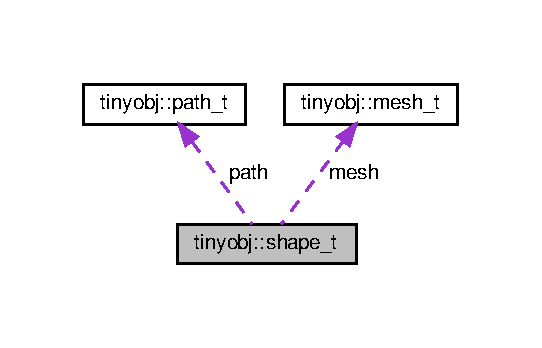
\includegraphics[width=260pt]{structtinyobj_1_1shape__t__coll__graph}
\end{center}
\end{figure}
\subsection*{Javni članovi}
\begin{DoxyCompactItemize}
\item 
std\+::string \hyperlink{structtinyobj_1_1shape__t_a98650e2e66d00934f68de88eafb34630}{name}
\item 
\hyperlink{structtinyobj_1_1mesh__t}{mesh\+\_\+t} \hyperlink{structtinyobj_1_1shape__t_a3dacb06dfbfe9e245ff4bc7b5b3d9818}{mesh}
\item 
\hyperlink{structtinyobj_1_1path__t}{path\+\_\+t} \hyperlink{structtinyobj_1_1shape__t_a3e25b80e1330260be137eb865ec0b958}{path}
\end{DoxyCompactItemize}


\subsection{Dokumentacija atributa}
\mbox{\Hypertarget{structtinyobj_1_1shape__t_a3dacb06dfbfe9e245ff4bc7b5b3d9818}\label{structtinyobj_1_1shape__t_a3dacb06dfbfe9e245ff4bc7b5b3d9818}} 
\index{tinyobj\+::shape\+\_\+t@{tinyobj\+::shape\+\_\+t}!mesh@{mesh}}
\index{mesh@{mesh}!tinyobj\+::shape\+\_\+t@{tinyobj\+::shape\+\_\+t}}
\subsubsection{\texorpdfstring{mesh}{mesh}}
{\footnotesize\ttfamily \hyperlink{structtinyobj_1_1mesh__t}{mesh\+\_\+t} tinyobj\+::shape\+\_\+t\+::mesh}

\mbox{\Hypertarget{structtinyobj_1_1shape__t_a98650e2e66d00934f68de88eafb34630}\label{structtinyobj_1_1shape__t_a98650e2e66d00934f68de88eafb34630}} 
\index{tinyobj\+::shape\+\_\+t@{tinyobj\+::shape\+\_\+t}!name@{name}}
\index{name@{name}!tinyobj\+::shape\+\_\+t@{tinyobj\+::shape\+\_\+t}}
\subsubsection{\texorpdfstring{name}{name}}
{\footnotesize\ttfamily std\+::string tinyobj\+::shape\+\_\+t\+::name}

\mbox{\Hypertarget{structtinyobj_1_1shape__t_a3e25b80e1330260be137eb865ec0b958}\label{structtinyobj_1_1shape__t_a3e25b80e1330260be137eb865ec0b958}} 
\index{tinyobj\+::shape\+\_\+t@{tinyobj\+::shape\+\_\+t}!path@{path}}
\index{path@{path}!tinyobj\+::shape\+\_\+t@{tinyobj\+::shape\+\_\+t}}
\subsubsection{\texorpdfstring{path}{path}}
{\footnotesize\ttfamily \hyperlink{structtinyobj_1_1path__t}{path\+\_\+t} tinyobj\+::shape\+\_\+t\+::path}



Dokumentacija ove strukture je napravljena na osnovu datoteke \begin{DoxyCompactItemize}
\item 
/home/dusan/\+Documents/\+R\+G146-\/vitez-\/reda-\/zmaja/include/external\+\_\+libs/\hyperlink{tiny__obj__loader_8h}{tiny\+\_\+obj\+\_\+loader.\+h}\end{DoxyCompactItemize}

\hypertarget{structtinyobj_1_1tag__t}{}\section{Dokumentacija strukture tinyobj\+:\+:tag\+\_\+t}
\label{structtinyobj_1_1tag__t}\index{tinyobj\+::tag\+\_\+t@{tinyobj\+::tag\+\_\+t}}


{\ttfamily \#include $<$tiny\+\_\+obj\+\_\+loader.\+h$>$}

\subsection*{Javni članovi}
\begin{DoxyCompactItemize}
\item 
std\+::string \hyperlink{structtinyobj_1_1tag__t_a9b3650154d2fbd83dad945ebcf6bd448}{name}
\item 
std\+::vector$<$ int $>$ \hyperlink{structtinyobj_1_1tag__t_adc6a6682263abaa11e3ec62b910bb80d}{int\+Values}
\item 
std\+::vector$<$ \hyperlink{namespacetinyobj_ad5ca7469ff56bf0d8423120cfd99adce}{real\+\_\+t} $>$ \hyperlink{structtinyobj_1_1tag__t_a6e531cc0a0d53b6334cf55da4bb62ffc}{float\+Values}
\item 
std\+::vector$<$ std\+::string $>$ \hyperlink{structtinyobj_1_1tag__t_a25634eea923961fd5b2520ea782397e8}{string\+Values}
\end{DoxyCompactItemize}


\subsection{Dokumentacija atributa}
\mbox{\Hypertarget{structtinyobj_1_1tag__t_a6e531cc0a0d53b6334cf55da4bb62ffc}\label{structtinyobj_1_1tag__t_a6e531cc0a0d53b6334cf55da4bb62ffc}} 
\index{tinyobj\+::tag\+\_\+t@{tinyobj\+::tag\+\_\+t}!float\+Values@{float\+Values}}
\index{float\+Values@{float\+Values}!tinyobj\+::tag\+\_\+t@{tinyobj\+::tag\+\_\+t}}
\subsubsection{\texorpdfstring{float\+Values}{floatValues}}
{\footnotesize\ttfamily std\+::vector$<$\hyperlink{namespacetinyobj_ad5ca7469ff56bf0d8423120cfd99adce}{real\+\_\+t}$>$ tinyobj\+::tag\+\_\+t\+::float\+Values}

\mbox{\Hypertarget{structtinyobj_1_1tag__t_adc6a6682263abaa11e3ec62b910bb80d}\label{structtinyobj_1_1tag__t_adc6a6682263abaa11e3ec62b910bb80d}} 
\index{tinyobj\+::tag\+\_\+t@{tinyobj\+::tag\+\_\+t}!int\+Values@{int\+Values}}
\index{int\+Values@{int\+Values}!tinyobj\+::tag\+\_\+t@{tinyobj\+::tag\+\_\+t}}
\subsubsection{\texorpdfstring{int\+Values}{intValues}}
{\footnotesize\ttfamily std\+::vector$<$int$>$ tinyobj\+::tag\+\_\+t\+::int\+Values}

\mbox{\Hypertarget{structtinyobj_1_1tag__t_a9b3650154d2fbd83dad945ebcf6bd448}\label{structtinyobj_1_1tag__t_a9b3650154d2fbd83dad945ebcf6bd448}} 
\index{tinyobj\+::tag\+\_\+t@{tinyobj\+::tag\+\_\+t}!name@{name}}
\index{name@{name}!tinyobj\+::tag\+\_\+t@{tinyobj\+::tag\+\_\+t}}
\subsubsection{\texorpdfstring{name}{name}}
{\footnotesize\ttfamily std\+::string tinyobj\+::tag\+\_\+t\+::name}

\mbox{\Hypertarget{structtinyobj_1_1tag__t_a25634eea923961fd5b2520ea782397e8}\label{structtinyobj_1_1tag__t_a25634eea923961fd5b2520ea782397e8}} 
\index{tinyobj\+::tag\+\_\+t@{tinyobj\+::tag\+\_\+t}!string\+Values@{string\+Values}}
\index{string\+Values@{string\+Values}!tinyobj\+::tag\+\_\+t@{tinyobj\+::tag\+\_\+t}}
\subsubsection{\texorpdfstring{string\+Values}{stringValues}}
{\footnotesize\ttfamily std\+::vector$<$std\+::string$>$ tinyobj\+::tag\+\_\+t\+::string\+Values}



Dokumentacija ove strukture je napravljena na osnovu datoteke \begin{DoxyCompactItemize}
\item 
/home/dusan/\+Documents/\+R\+G146-\/vitez-\/reda-\/zmaja/include/external\+\_\+libs/\hyperlink{tiny__obj__loader_8h}{tiny\+\_\+obj\+\_\+loader.\+h}\end{DoxyCompactItemize}

\hypertarget{classterrain_1_1Terrain}{}\section{Dokumentacija klase terrain\+:\+:Terrain}
\label{classterrain_1_1Terrain}\index{terrain\+::\+Terrain@{terrain\+::\+Terrain}}


{\ttfamily \#include $<$Terrain.\+h$>$}



Klasni dijagram za terrain\+:\+:Terrain\+:
\nopagebreak
\begin{figure}[H]
\begin{center}
\leavevmode
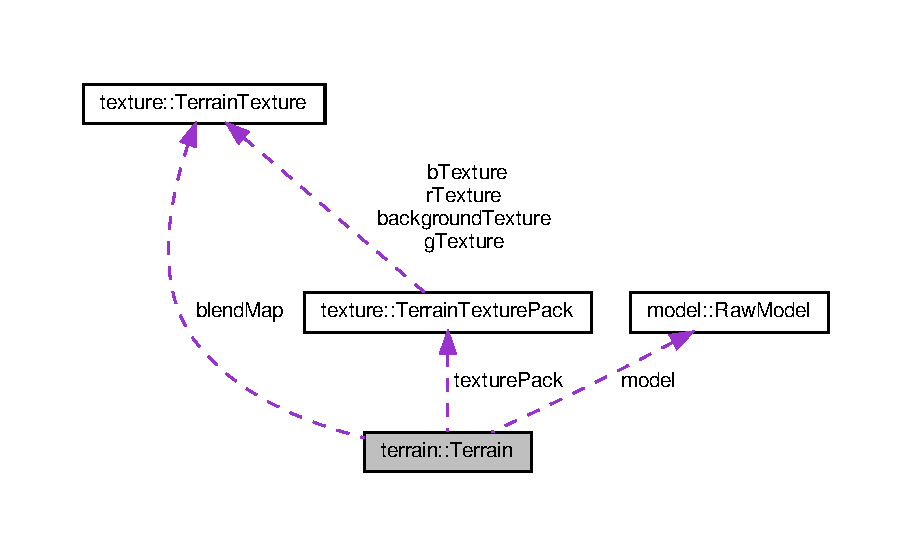
\includegraphics[width=350pt]{classterrain_1_1Terrain__coll__graph}
\end{center}
\end{figure}
\subsection*{Javni članovi}
\begin{DoxyCompactItemize}
\item 
\hyperlink{classterrain_1_1Terrain_a3361d2b8405cb829d0b851a944bce94b}{Terrain} (float gridX, float gridZ, \hyperlink{classcore_1_1VaoLoader}{Vao\+Loader} $\ast$vao\+Loader, \hyperlink{classtexture_1_1TerrainTexturePack}{Terrain\+Texture\+Pack} $\ast$\hyperlink{classterrain_1_1Terrain_a6f9e86bd4c98ec61c9588b9f2b57fb75}{texture\+Pack}, \hyperlink{classtexture_1_1TerrainTexture}{Terrain\+Texture} $\ast$\hyperlink{classterrain_1_1Terrain_a48d20417020f61e62bb5d3a497c62a57}{blend\+Map}, const char $\ast$height\+Map)
\item 
\hyperlink{classterrain_1_1Terrain_a6aa3821700c2010298c1ad9f83971670}{$\sim$\+Terrain} ()
\item 
\hyperlink{classmodel_1_1RawModel}{Raw\+Model} $\ast$ \hyperlink{classterrain_1_1Terrain_a336c5efe16ff0fd81c8b6b6f00b9ba08}{get\+Model} ()
\item 
\hyperlink{classtexture_1_1TerrainTexturePack}{Terrain\+Texture\+Pack} $\ast$ \hyperlink{classterrain_1_1Terrain_a6b6100654d9bb6f5f5ea004cc5bf95f4}{get\+Texture\+Pack} ()
\item 
\hyperlink{classtexture_1_1TerrainTexture}{Terrain\+Texture} $\ast$ \hyperlink{classterrain_1_1Terrain_ae4d64fa4f81168a02887127491572cef}{get\+Blend\+Map} ()
\item 
float \hyperlink{classterrain_1_1Terrain_a7498906e811d059461be143d7323a6f9}{getX} ()
\item 
float \hyperlink{classterrain_1_1Terrain_ab348a1c250df237f2a60f59bf8797dc0}{getZ} ()
\item 
float \hyperlink{classterrain_1_1Terrain_afd074b9a18254b81abb89d29406f90e5}{get\+Height\+Of\+Terrain} (int worldX, int worldZ)
\end{DoxyCompactItemize}
\subsection*{Privatni članovi}
\begin{DoxyCompactItemize}
\item 
vec3 \hyperlink{classterrain_1_1Terrain_a2864540ccf7224830c0bbf2961d207bb}{calculate\+Normal} (Image image, int \hyperlink{classterrain_1_1Terrain_aec56d6e8219539617090b8e99b89be29}{x}, int y)
\item 
float \hyperlink{classterrain_1_1Terrain_a0707a64c79d89cfc358670651855cba1}{get\+Height} (Image image, int \hyperlink{classterrain_1_1Terrain_aec56d6e8219539617090b8e99b89be29}{x}, int y)
\item 
\hyperlink{classmodel_1_1RawModel}{Raw\+Model} $\ast$ \hyperlink{classterrain_1_1Terrain_aadecc14ee7c1c340c54c6960d489f1da}{generate\+Terrain} (\hyperlink{classcore_1_1VaoLoader}{Vao\+Loader} $\ast$vao\+Loader, Image image)
\end{DoxyCompactItemize}
\subsection*{Privatni članovi}
\begin{DoxyCompactItemize}
\item 
float \hyperlink{classterrain_1_1Terrain_aec56d6e8219539617090b8e99b89be29}{x}
\item 
float \hyperlink{classterrain_1_1Terrain_aaa4c36ce01096f81a0ee174c36f19657}{z}
\item 
\hyperlink{classmodel_1_1RawModel}{Raw\+Model} $\ast$ \hyperlink{classterrain_1_1Terrain_a0811e4548a966a38b3ca6a4475666324}{model}
\item 
\hyperlink{classtexture_1_1TerrainTexturePack}{Terrain\+Texture\+Pack} $\ast$ \hyperlink{classterrain_1_1Terrain_a6f9e86bd4c98ec61c9588b9f2b57fb75}{texture\+Pack}
\item 
\hyperlink{classtexture_1_1TerrainTexture}{Terrain\+Texture} $\ast$ \hyperlink{classterrain_1_1Terrain_a48d20417020f61e62bb5d3a497c62a57}{blend\+Map}
\item 
float $\ast$$\ast$ \hyperlink{classterrain_1_1Terrain_a068874d68315a2dafb59630e6d9410f1}{heights}
\item 
int \hyperlink{classterrain_1_1Terrain_a797e69c6650b5870643574625f853718}{heights\+Length}
\item 
int \hyperlink{classterrain_1_1Terrain_a27ca93bfb1ba44b0ff2935d667614f71}{V\+E\+R\+T\+E\+X\+\_\+\+C\+O\+U\+NT}
\end{DoxyCompactItemize}


\subsection{Dokumentacija konstruktora i destruktora}
\mbox{\Hypertarget{classterrain_1_1Terrain_a3361d2b8405cb829d0b851a944bce94b}\label{classterrain_1_1Terrain_a3361d2b8405cb829d0b851a944bce94b}} 
\index{terrain\+::\+Terrain@{terrain\+::\+Terrain}!Terrain@{Terrain}}
\index{Terrain@{Terrain}!terrain\+::\+Terrain@{terrain\+::\+Terrain}}
\subsubsection{\texorpdfstring{Terrain()}{Terrain()}}
{\footnotesize\ttfamily terrain\+::\+Terrain\+::\+Terrain (\begin{DoxyParamCaption}\item[{float}]{gridX,  }\item[{float}]{gridZ,  }\item[{\hyperlink{classcore_1_1VaoLoader}{Vao\+Loader} $\ast$}]{vao\+Loader,  }\item[{\hyperlink{classtexture_1_1TerrainTexturePack}{Terrain\+Texture\+Pack} $\ast$}]{texture\+Pack,  }\item[{\hyperlink{classtexture_1_1TerrainTexture}{Terrain\+Texture} $\ast$}]{blend\+Map,  }\item[{const char $\ast$}]{height\+Map }\end{DoxyParamCaption})}

\mbox{\Hypertarget{classterrain_1_1Terrain_a6aa3821700c2010298c1ad9f83971670}\label{classterrain_1_1Terrain_a6aa3821700c2010298c1ad9f83971670}} 
\index{terrain\+::\+Terrain@{terrain\+::\+Terrain}!````~Terrain@{$\sim$\+Terrain}}
\index{````~Terrain@{$\sim$\+Terrain}!terrain\+::\+Terrain@{terrain\+::\+Terrain}}
\subsubsection{\texorpdfstring{$\sim$\+Terrain()}{~Terrain()}}
{\footnotesize\ttfamily terrain\+::\+Terrain\+::$\sim$\+Terrain (\begin{DoxyParamCaption}{ }\end{DoxyParamCaption})}



\subsection{Dokumentacija funkcija članica}
\mbox{\Hypertarget{classterrain_1_1Terrain_a2864540ccf7224830c0bbf2961d207bb}\label{classterrain_1_1Terrain_a2864540ccf7224830c0bbf2961d207bb}} 
\index{terrain\+::\+Terrain@{terrain\+::\+Terrain}!calculate\+Normal@{calculate\+Normal}}
\index{calculate\+Normal@{calculate\+Normal}!terrain\+::\+Terrain@{terrain\+::\+Terrain}}
\subsubsection{\texorpdfstring{calculate\+Normal()}{calculateNormal()}}
{\footnotesize\ttfamily vec3 terrain\+::\+Terrain\+::calculate\+Normal (\begin{DoxyParamCaption}\item[{Image}]{image,  }\item[{int}]{x,  }\item[{int}]{y }\end{DoxyParamCaption})\hspace{0.3cm}{\ttfamily [private]}}

\mbox{\Hypertarget{classterrain_1_1Terrain_aadecc14ee7c1c340c54c6960d489f1da}\label{classterrain_1_1Terrain_aadecc14ee7c1c340c54c6960d489f1da}} 
\index{terrain\+::\+Terrain@{terrain\+::\+Terrain}!generate\+Terrain@{generate\+Terrain}}
\index{generate\+Terrain@{generate\+Terrain}!terrain\+::\+Terrain@{terrain\+::\+Terrain}}
\subsubsection{\texorpdfstring{generate\+Terrain()}{generateTerrain()}}
{\footnotesize\ttfamily \hyperlink{classmodel_1_1RawModel}{Raw\+Model} $\ast$ terrain\+::\+Terrain\+::generate\+Terrain (\begin{DoxyParamCaption}\item[{\hyperlink{classcore_1_1VaoLoader}{Vao\+Loader} $\ast$}]{vao\+Loader,  }\item[{Image}]{image }\end{DoxyParamCaption})\hspace{0.3cm}{\ttfamily [private]}}

\mbox{\Hypertarget{classterrain_1_1Terrain_ae4d64fa4f81168a02887127491572cef}\label{classterrain_1_1Terrain_ae4d64fa4f81168a02887127491572cef}} 
\index{terrain\+::\+Terrain@{terrain\+::\+Terrain}!get\+Blend\+Map@{get\+Blend\+Map}}
\index{get\+Blend\+Map@{get\+Blend\+Map}!terrain\+::\+Terrain@{terrain\+::\+Terrain}}
\subsubsection{\texorpdfstring{get\+Blend\+Map()}{getBlendMap()}}
{\footnotesize\ttfamily \hyperlink{classtexture_1_1TerrainTexture}{Terrain\+Texture} $\ast$ terrain\+::\+Terrain\+::get\+Blend\+Map (\begin{DoxyParamCaption}{ }\end{DoxyParamCaption})}

\mbox{\Hypertarget{classterrain_1_1Terrain_a0707a64c79d89cfc358670651855cba1}\label{classterrain_1_1Terrain_a0707a64c79d89cfc358670651855cba1}} 
\index{terrain\+::\+Terrain@{terrain\+::\+Terrain}!get\+Height@{get\+Height}}
\index{get\+Height@{get\+Height}!terrain\+::\+Terrain@{terrain\+::\+Terrain}}
\subsubsection{\texorpdfstring{get\+Height()}{getHeight()}}
{\footnotesize\ttfamily float terrain\+::\+Terrain\+::get\+Height (\begin{DoxyParamCaption}\item[{Image}]{image,  }\item[{int}]{x,  }\item[{int}]{y }\end{DoxyParamCaption})\hspace{0.3cm}{\ttfamily [private]}}

\mbox{\Hypertarget{classterrain_1_1Terrain_afd074b9a18254b81abb89d29406f90e5}\label{classterrain_1_1Terrain_afd074b9a18254b81abb89d29406f90e5}} 
\index{terrain\+::\+Terrain@{terrain\+::\+Terrain}!get\+Height\+Of\+Terrain@{get\+Height\+Of\+Terrain}}
\index{get\+Height\+Of\+Terrain@{get\+Height\+Of\+Terrain}!terrain\+::\+Terrain@{terrain\+::\+Terrain}}
\subsubsection{\texorpdfstring{get\+Height\+Of\+Terrain()}{getHeightOfTerrain()}}
{\footnotesize\ttfamily float terrain\+::\+Terrain\+::get\+Height\+Of\+Terrain (\begin{DoxyParamCaption}\item[{int}]{worldX,  }\item[{int}]{worldZ }\end{DoxyParamCaption})}

\mbox{\Hypertarget{classterrain_1_1Terrain_a336c5efe16ff0fd81c8b6b6f00b9ba08}\label{classterrain_1_1Terrain_a336c5efe16ff0fd81c8b6b6f00b9ba08}} 
\index{terrain\+::\+Terrain@{terrain\+::\+Terrain}!get\+Model@{get\+Model}}
\index{get\+Model@{get\+Model}!terrain\+::\+Terrain@{terrain\+::\+Terrain}}
\subsubsection{\texorpdfstring{get\+Model()}{getModel()}}
{\footnotesize\ttfamily \hyperlink{classmodel_1_1RawModel}{Raw\+Model} $\ast$ terrain\+::\+Terrain\+::get\+Model (\begin{DoxyParamCaption}{ }\end{DoxyParamCaption})}

\mbox{\Hypertarget{classterrain_1_1Terrain_a6b6100654d9bb6f5f5ea004cc5bf95f4}\label{classterrain_1_1Terrain_a6b6100654d9bb6f5f5ea004cc5bf95f4}} 
\index{terrain\+::\+Terrain@{terrain\+::\+Terrain}!get\+Texture\+Pack@{get\+Texture\+Pack}}
\index{get\+Texture\+Pack@{get\+Texture\+Pack}!terrain\+::\+Terrain@{terrain\+::\+Terrain}}
\subsubsection{\texorpdfstring{get\+Texture\+Pack()}{getTexturePack()}}
{\footnotesize\ttfamily \hyperlink{classtexture_1_1TerrainTexturePack}{Terrain\+Texture\+Pack} $\ast$ terrain\+::\+Terrain\+::get\+Texture\+Pack (\begin{DoxyParamCaption}{ }\end{DoxyParamCaption})}

\mbox{\Hypertarget{classterrain_1_1Terrain_a7498906e811d059461be143d7323a6f9}\label{classterrain_1_1Terrain_a7498906e811d059461be143d7323a6f9}} 
\index{terrain\+::\+Terrain@{terrain\+::\+Terrain}!getX@{getX}}
\index{getX@{getX}!terrain\+::\+Terrain@{terrain\+::\+Terrain}}
\subsubsection{\texorpdfstring{get\+X()}{getX()}}
{\footnotesize\ttfamily float terrain\+::\+Terrain\+::getX (\begin{DoxyParamCaption}{ }\end{DoxyParamCaption})}

\mbox{\Hypertarget{classterrain_1_1Terrain_ab348a1c250df237f2a60f59bf8797dc0}\label{classterrain_1_1Terrain_ab348a1c250df237f2a60f59bf8797dc0}} 
\index{terrain\+::\+Terrain@{terrain\+::\+Terrain}!getZ@{getZ}}
\index{getZ@{getZ}!terrain\+::\+Terrain@{terrain\+::\+Terrain}}
\subsubsection{\texorpdfstring{get\+Z()}{getZ()}}
{\footnotesize\ttfamily float terrain\+::\+Terrain\+::getZ (\begin{DoxyParamCaption}{ }\end{DoxyParamCaption})}



\subsection{Dokumentacija atributa}
\mbox{\Hypertarget{classterrain_1_1Terrain_a48d20417020f61e62bb5d3a497c62a57}\label{classterrain_1_1Terrain_a48d20417020f61e62bb5d3a497c62a57}} 
\index{terrain\+::\+Terrain@{terrain\+::\+Terrain}!blend\+Map@{blend\+Map}}
\index{blend\+Map@{blend\+Map}!terrain\+::\+Terrain@{terrain\+::\+Terrain}}
\subsubsection{\texorpdfstring{blend\+Map}{blendMap}}
{\footnotesize\ttfamily \hyperlink{classtexture_1_1TerrainTexture}{Terrain\+Texture}$\ast$ terrain\+::\+Terrain\+::blend\+Map\hspace{0.3cm}{\ttfamily [private]}}

\mbox{\Hypertarget{classterrain_1_1Terrain_a068874d68315a2dafb59630e6d9410f1}\label{classterrain_1_1Terrain_a068874d68315a2dafb59630e6d9410f1}} 
\index{terrain\+::\+Terrain@{terrain\+::\+Terrain}!heights@{heights}}
\index{heights@{heights}!terrain\+::\+Terrain@{terrain\+::\+Terrain}}
\subsubsection{\texorpdfstring{heights}{heights}}
{\footnotesize\ttfamily float$\ast$$\ast$ terrain\+::\+Terrain\+::heights\hspace{0.3cm}{\ttfamily [private]}}

\mbox{\Hypertarget{classterrain_1_1Terrain_a797e69c6650b5870643574625f853718}\label{classterrain_1_1Terrain_a797e69c6650b5870643574625f853718}} 
\index{terrain\+::\+Terrain@{terrain\+::\+Terrain}!heights\+Length@{heights\+Length}}
\index{heights\+Length@{heights\+Length}!terrain\+::\+Terrain@{terrain\+::\+Terrain}}
\subsubsection{\texorpdfstring{heights\+Length}{heightsLength}}
{\footnotesize\ttfamily int terrain\+::\+Terrain\+::heights\+Length\hspace{0.3cm}{\ttfamily [private]}}

\mbox{\Hypertarget{classterrain_1_1Terrain_a0811e4548a966a38b3ca6a4475666324}\label{classterrain_1_1Terrain_a0811e4548a966a38b3ca6a4475666324}} 
\index{terrain\+::\+Terrain@{terrain\+::\+Terrain}!model@{model}}
\index{model@{model}!terrain\+::\+Terrain@{terrain\+::\+Terrain}}
\subsubsection{\texorpdfstring{model}{model}}
{\footnotesize\ttfamily \hyperlink{classmodel_1_1RawModel}{Raw\+Model}$\ast$ terrain\+::\+Terrain\+::model\hspace{0.3cm}{\ttfamily [private]}}

\mbox{\Hypertarget{classterrain_1_1Terrain_a6f9e86bd4c98ec61c9588b9f2b57fb75}\label{classterrain_1_1Terrain_a6f9e86bd4c98ec61c9588b9f2b57fb75}} 
\index{terrain\+::\+Terrain@{terrain\+::\+Terrain}!texture\+Pack@{texture\+Pack}}
\index{texture\+Pack@{texture\+Pack}!terrain\+::\+Terrain@{terrain\+::\+Terrain}}
\subsubsection{\texorpdfstring{texture\+Pack}{texturePack}}
{\footnotesize\ttfamily \hyperlink{classtexture_1_1TerrainTexturePack}{Terrain\+Texture\+Pack}$\ast$ terrain\+::\+Terrain\+::texture\+Pack\hspace{0.3cm}{\ttfamily [private]}}

\mbox{\Hypertarget{classterrain_1_1Terrain_a27ca93bfb1ba44b0ff2935d667614f71}\label{classterrain_1_1Terrain_a27ca93bfb1ba44b0ff2935d667614f71}} 
\index{terrain\+::\+Terrain@{terrain\+::\+Terrain}!V\+E\+R\+T\+E\+X\+\_\+\+C\+O\+U\+NT@{V\+E\+R\+T\+E\+X\+\_\+\+C\+O\+U\+NT}}
\index{V\+E\+R\+T\+E\+X\+\_\+\+C\+O\+U\+NT@{V\+E\+R\+T\+E\+X\+\_\+\+C\+O\+U\+NT}!terrain\+::\+Terrain@{terrain\+::\+Terrain}}
\subsubsection{\texorpdfstring{V\+E\+R\+T\+E\+X\+\_\+\+C\+O\+U\+NT}{VERTEX\_COUNT}}
{\footnotesize\ttfamily int terrain\+::\+Terrain\+::\+V\+E\+R\+T\+E\+X\+\_\+\+C\+O\+U\+NT\hspace{0.3cm}{\ttfamily [private]}}

\mbox{\Hypertarget{classterrain_1_1Terrain_aec56d6e8219539617090b8e99b89be29}\label{classterrain_1_1Terrain_aec56d6e8219539617090b8e99b89be29}} 
\index{terrain\+::\+Terrain@{terrain\+::\+Terrain}!x@{x}}
\index{x@{x}!terrain\+::\+Terrain@{terrain\+::\+Terrain}}
\subsubsection{\texorpdfstring{x}{x}}
{\footnotesize\ttfamily float terrain\+::\+Terrain\+::x\hspace{0.3cm}{\ttfamily [private]}}

\mbox{\Hypertarget{classterrain_1_1Terrain_aaa4c36ce01096f81a0ee174c36f19657}\label{classterrain_1_1Terrain_aaa4c36ce01096f81a0ee174c36f19657}} 
\index{terrain\+::\+Terrain@{terrain\+::\+Terrain}!z@{z}}
\index{z@{z}!terrain\+::\+Terrain@{terrain\+::\+Terrain}}
\subsubsection{\texorpdfstring{z}{z}}
{\footnotesize\ttfamily float terrain\+::\+Terrain\+::z\hspace{0.3cm}{\ttfamily [private]}}



Dokumentacija ove klase je napravljena na osnovu sledećih datoteka\+:\begin{DoxyCompactItemize}
\item 
/home/dusan/\+Documents/\+Projects/\+R\+G102-\/vitez-\/reda-\/zmaja/include/terrain/\hyperlink{Terrain_8h}{Terrain.\+h}\item 
/home/dusan/\+Documents/\+Projects/\+R\+G102-\/vitez-\/reda-\/zmaja/src/terrain/\hyperlink{Terrain_8cpp}{Terrain.\+cpp}\end{DoxyCompactItemize}

\hypertarget{classcore_1_1TerrainRenderer}{}\section{Dokumentacija klase core\+:\+:Terrain\+Renderer}
\label{classcore_1_1TerrainRenderer}\index{core\+::\+Terrain\+Renderer@{core\+::\+Terrain\+Renderer}}


Klasa \hyperlink{classcore_1_1TerrainRenderer}{Terrain\+Renderer} je zaduzena za iscrtavanje terena na ekran. Tokom pokretanja prvo se vrsi priprema za iscrtavanje, a zatim se sadrzaj niza atributa(koordinate, boje, texture ...) iscrtava na ekran.  




{\ttfamily \#include $<$Terrain\+Renderer.\+h$>$}



Klasni dijagram za core\+:\+:Terrain\+Renderer\+:\nopagebreak
\begin{figure}[H]
\begin{center}
\leavevmode
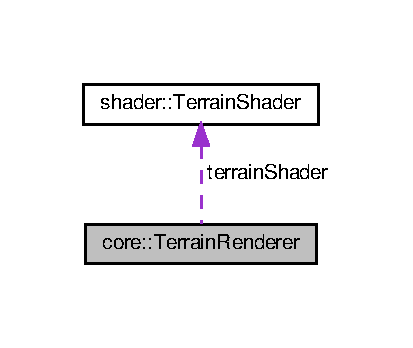
\includegraphics[width=198pt]{classcore_1_1TerrainRenderer__coll__graph}
\end{center}
\end{figure}
\subsection*{Javni članovi}
\begin{DoxyCompactItemize}
\item 
\hyperlink{classcore_1_1TerrainRenderer_aef52c32054bf2be3fc5ec160a2d7433b}{Terrain\+Renderer} (\hyperlink{classshader_1_1TerrainShader}{Terrain\+Shader} $\ast$\hyperlink{classcore_1_1TerrainRenderer_a6db721ffef6f7175977ad243b4ac2834}{terrain\+Shader})
\begin{DoxyCompactList}\small\item\em Konstruktor klase. \end{DoxyCompactList}\item 
\hyperlink{classcore_1_1TerrainRenderer_a18e79e2c14c4f2196d410bbde7b85060}{$\sim$\+Terrain\+Renderer} ()
\begin{DoxyCompactList}\small\item\em Destruktor klase. \end{DoxyCompactList}\item 
void \hyperlink{classcore_1_1TerrainRenderer_a1f2aaf851e780fc8f78aa5bb3cd1b512}{render} (list$<$ \hyperlink{classterrain_1_1Terrain}{Terrain} $\ast$$>$ terrains)
\begin{DoxyCompactList}\small\item\em Funkcija iscrtava terene na ekran. \end{DoxyCompactList}\item 
void \hyperlink{classcore_1_1TerrainRenderer_ad4e7d88767cdfc19ee07bf3558f6c1f0}{prepare\+Terrain} (\hyperlink{classterrain_1_1Terrain}{Terrain} $\ast$\hyperlink{namespacecore_ac45da6f80dac9bead5c9310c27897f15}{terrain})
\begin{DoxyCompactList}\small\item\em Funkcija vrsi pripremu terena za ucitavanje. \end{DoxyCompactList}\item 
void \hyperlink{classcore_1_1TerrainRenderer_ac66bf45a30d7c1b443f8b77132112fe0}{bind\+Textures} (\hyperlink{classterrain_1_1Terrain}{Terrain} $\ast$\hyperlink{namespacecore_ac45da6f80dac9bead5c9310c27897f15}{terrain})
\begin{DoxyCompactList}\small\item\em Funkcija povezuje teksture terena. \end{DoxyCompactList}\item 
void \hyperlink{classcore_1_1TerrainRenderer_ac739a96169a8fef7bfad56bbe3367962}{unbind\+Terrain} ()
\begin{DoxyCompactList}\small\item\em Funkcija otklanja vezu izmedju podataka terena i programa. \end{DoxyCompactList}\item 
void \hyperlink{classcore_1_1TerrainRenderer_a5e1837566f4de6e49dbf19e203cc9563}{load\+Model\+Matrix} (\hyperlink{classterrain_1_1Terrain}{Terrain} $\ast$\hyperlink{namespacecore_ac45da6f80dac9bead5c9310c27897f15}{terrain})
\begin{DoxyCompactList}\small\item\em Funkcija kreira matricu transformacije za teren i ucitava je u sejder program. \end{DoxyCompactList}\end{DoxyCompactItemize}
\subsection*{Privatni članovi}
\begin{DoxyCompactItemize}
\item 
mat4 \hyperlink{classcore_1_1TerrainRenderer_a06f89d76316964a8da14498ec43756f0}{create\+Projection\+Matrix} ()
\begin{DoxyCompactList}\small\item\em Funkcija kreira matricu projekcije. \end{DoxyCompactList}\end{DoxyCompactItemize}
\subsection*{Privatni članovi}
\begin{DoxyCompactItemize}
\item 
float \hyperlink{classcore_1_1TerrainRenderer_a912eab623ca8c7ca7d8473e30383f831}{F\+OV} = 70
\begin{DoxyCompactList}\small\item\em Polje vidika. \end{DoxyCompactList}\item 
float \hyperlink{classcore_1_1TerrainRenderer_a68bdfd4b42381b4514991fe8c4d08c89}{N\+E\+A\+R\+\_\+\+P\+L\+A\+NE} = 0.\+1
\begin{DoxyCompactList}\small\item\em Prednji deo vidljivosti. \end{DoxyCompactList}\item 
float \hyperlink{classcore_1_1TerrainRenderer_abc56752e01a0b9b0ebfd57b8daa6172c}{F\+A\+R\+\_\+\+P\+L\+A\+NE} = 1000
\begin{DoxyCompactList}\small\item\em Zadnji deo vidljivosti. \end{DoxyCompactList}\item 
\hyperlink{classshader_1_1TerrainShader}{Terrain\+Shader} $\ast$ \hyperlink{classcore_1_1TerrainRenderer_a6db721ffef6f7175977ad243b4ac2834}{terrain\+Shader}
\begin{DoxyCompactList}\small\item\em Pokazivac na instancu klase Terrain\+Shader. \end{DoxyCompactList}\end{DoxyCompactItemize}


\subsection{Opširniji opis}
Klasa \hyperlink{classcore_1_1TerrainRenderer}{Terrain\+Renderer} je zaduzena za iscrtavanje terena na ekran. Tokom pokretanja prvo se vrsi priprema za iscrtavanje, a zatim se sadrzaj niza atributa(koordinate, boje, texture ...) iscrtava na ekran. 

\subsection{Dokumentacija konstruktora i destruktora}
\mbox{\Hypertarget{classcore_1_1TerrainRenderer_aef52c32054bf2be3fc5ec160a2d7433b}\label{classcore_1_1TerrainRenderer_aef52c32054bf2be3fc5ec160a2d7433b}} 
\index{core\+::\+Terrain\+Renderer@{core\+::\+Terrain\+Renderer}!Terrain\+Renderer@{Terrain\+Renderer}}
\index{Terrain\+Renderer@{Terrain\+Renderer}!core\+::\+Terrain\+Renderer@{core\+::\+Terrain\+Renderer}}
\subsubsection{\texorpdfstring{Terrain\+Renderer()}{TerrainRenderer()}}
{\footnotesize\ttfamily core\+::\+Terrain\+Renderer\+::\+Terrain\+Renderer (\begin{DoxyParamCaption}\item[{\hyperlink{classshader_1_1TerrainShader}{Terrain\+Shader} $\ast$}]{terrain\+Shader }\end{DoxyParamCaption})}



Konstruktor klase. 


\begin{DoxyParams}{Parametri}
{\em terrain\+Shader} & Pokazivac na instancu klase Terrain\+Shader. \\
\hline
\end{DoxyParams}
\mbox{\Hypertarget{classcore_1_1TerrainRenderer_a18e79e2c14c4f2196d410bbde7b85060}\label{classcore_1_1TerrainRenderer_a18e79e2c14c4f2196d410bbde7b85060}} 
\index{core\+::\+Terrain\+Renderer@{core\+::\+Terrain\+Renderer}!````~Terrain\+Renderer@{$\sim$\+Terrain\+Renderer}}
\index{````~Terrain\+Renderer@{$\sim$\+Terrain\+Renderer}!core\+::\+Terrain\+Renderer@{core\+::\+Terrain\+Renderer}}
\subsubsection{\texorpdfstring{$\sim$\+Terrain\+Renderer()}{~TerrainRenderer()}}
{\footnotesize\ttfamily core\+::\+Terrain\+Renderer\+::$\sim$\+Terrain\+Renderer (\begin{DoxyParamCaption}{ }\end{DoxyParamCaption})}



Destruktor klase. 


\begin{DoxyParams}{Parametri}
{\em void} & \\
\hline
\end{DoxyParams}


\subsection{Dokumentacija funkcija članica}
\mbox{\Hypertarget{classcore_1_1TerrainRenderer_ac66bf45a30d7c1b443f8b77132112fe0}\label{classcore_1_1TerrainRenderer_ac66bf45a30d7c1b443f8b77132112fe0}} 
\index{core\+::\+Terrain\+Renderer@{core\+::\+Terrain\+Renderer}!bind\+Textures@{bind\+Textures}}
\index{bind\+Textures@{bind\+Textures}!core\+::\+Terrain\+Renderer@{core\+::\+Terrain\+Renderer}}
\subsubsection{\texorpdfstring{bind\+Textures()}{bindTextures()}}
{\footnotesize\ttfamily void core\+::\+Terrain\+Renderer\+::bind\+Textures (\begin{DoxyParamCaption}\item[{\hyperlink{classterrain_1_1Terrain}{Terrain} $\ast$}]{terrain }\end{DoxyParamCaption})}



Funkcija povezuje teksture terena. 


\begin{DoxyParams}{Parametri}
{\em terrain} & Pokazivac na instancu klase Terrain. \\
\hline
\end{DoxyParams}
\begin{DoxyReturn}{Vrednost funkcije}
void 
\end{DoxyReturn}
\mbox{\Hypertarget{classcore_1_1TerrainRenderer_a06f89d76316964a8da14498ec43756f0}\label{classcore_1_1TerrainRenderer_a06f89d76316964a8da14498ec43756f0}} 
\index{core\+::\+Terrain\+Renderer@{core\+::\+Terrain\+Renderer}!create\+Projection\+Matrix@{create\+Projection\+Matrix}}
\index{create\+Projection\+Matrix@{create\+Projection\+Matrix}!core\+::\+Terrain\+Renderer@{core\+::\+Terrain\+Renderer}}
\subsubsection{\texorpdfstring{create\+Projection\+Matrix()}{createProjectionMatrix()}}
{\footnotesize\ttfamily mat4 core\+::\+Terrain\+Renderer\+::create\+Projection\+Matrix (\begin{DoxyParamCaption}{ }\end{DoxyParamCaption})\hspace{0.3cm}{\ttfamily [private]}}



Funkcija kreira matricu projekcije. 


\begin{DoxyParams}{Parametri}
{\em void} & \\
\hline
\end{DoxyParams}
\begin{DoxyReturn}{Vrednost funkcije}
mat4 Matrica projekcije. 
\end{DoxyReturn}
\mbox{\Hypertarget{classcore_1_1TerrainRenderer_a5e1837566f4de6e49dbf19e203cc9563}\label{classcore_1_1TerrainRenderer_a5e1837566f4de6e49dbf19e203cc9563}} 
\index{core\+::\+Terrain\+Renderer@{core\+::\+Terrain\+Renderer}!load\+Model\+Matrix@{load\+Model\+Matrix}}
\index{load\+Model\+Matrix@{load\+Model\+Matrix}!core\+::\+Terrain\+Renderer@{core\+::\+Terrain\+Renderer}}
\subsubsection{\texorpdfstring{load\+Model\+Matrix()}{loadModelMatrix()}}
{\footnotesize\ttfamily void core\+::\+Terrain\+Renderer\+::load\+Model\+Matrix (\begin{DoxyParamCaption}\item[{\hyperlink{classterrain_1_1Terrain}{Terrain} $\ast$}]{terrain }\end{DoxyParamCaption})}



Funkcija kreira matricu transformacije za teren i ucitava je u sejder program. 


\begin{DoxyParams}{Parametri}
{\em terrain} & Pokazivac na instancu klase Terrain. \\
\hline
\end{DoxyParams}
\begin{DoxyReturn}{Vrednost funkcije}
void 
\end{DoxyReturn}
\mbox{\Hypertarget{classcore_1_1TerrainRenderer_ad4e7d88767cdfc19ee07bf3558f6c1f0}\label{classcore_1_1TerrainRenderer_ad4e7d88767cdfc19ee07bf3558f6c1f0}} 
\index{core\+::\+Terrain\+Renderer@{core\+::\+Terrain\+Renderer}!prepare\+Terrain@{prepare\+Terrain}}
\index{prepare\+Terrain@{prepare\+Terrain}!core\+::\+Terrain\+Renderer@{core\+::\+Terrain\+Renderer}}
\subsubsection{\texorpdfstring{prepare\+Terrain()}{prepareTerrain()}}
{\footnotesize\ttfamily void core\+::\+Terrain\+Renderer\+::prepare\+Terrain (\begin{DoxyParamCaption}\item[{\hyperlink{classterrain_1_1Terrain}{Terrain} $\ast$}]{terrain }\end{DoxyParamCaption})}



Funkcija vrsi pripremu terena za ucitavanje. 


\begin{DoxyParams}{Parametri}
{\em terrain} & Pokazivac na instancu klase Terrain. \\
\hline
\end{DoxyParams}
\begin{DoxyReturn}{Vrednost funkcije}
void 
\end{DoxyReturn}
\mbox{\Hypertarget{classcore_1_1TerrainRenderer_a1f2aaf851e780fc8f78aa5bb3cd1b512}\label{classcore_1_1TerrainRenderer_a1f2aaf851e780fc8f78aa5bb3cd1b512}} 
\index{core\+::\+Terrain\+Renderer@{core\+::\+Terrain\+Renderer}!render@{render}}
\index{render@{render}!core\+::\+Terrain\+Renderer@{core\+::\+Terrain\+Renderer}}
\subsubsection{\texorpdfstring{render()}{render()}}
{\footnotesize\ttfamily void core\+::\+Terrain\+Renderer\+::render (\begin{DoxyParamCaption}\item[{list$<$ \hyperlink{classterrain_1_1Terrain}{Terrain} $\ast$$>$}]{terrains }\end{DoxyParamCaption})}



Funkcija iscrtava terene na ekran. 


\begin{DoxyParams}{Parametri}
{\em terrains} & Lista terena. \\
\hline
\end{DoxyParams}
\begin{DoxyReturn}{Vrednost funkcije}
void 
\end{DoxyReturn}
\mbox{\Hypertarget{classcore_1_1TerrainRenderer_ac739a96169a8fef7bfad56bbe3367962}\label{classcore_1_1TerrainRenderer_ac739a96169a8fef7bfad56bbe3367962}} 
\index{core\+::\+Terrain\+Renderer@{core\+::\+Terrain\+Renderer}!unbind\+Terrain@{unbind\+Terrain}}
\index{unbind\+Terrain@{unbind\+Terrain}!core\+::\+Terrain\+Renderer@{core\+::\+Terrain\+Renderer}}
\subsubsection{\texorpdfstring{unbind\+Terrain()}{unbindTerrain()}}
{\footnotesize\ttfamily void core\+::\+Terrain\+Renderer\+::unbind\+Terrain (\begin{DoxyParamCaption}{ }\end{DoxyParamCaption})}



Funkcija otklanja vezu izmedju podataka terena i programa. 


\begin{DoxyParams}{Parametri}
{\em void} & \\
\hline
\end{DoxyParams}
\begin{DoxyReturn}{Vrednost funkcije}
void 
\end{DoxyReturn}


\subsection{Dokumentacija atributa}
\mbox{\Hypertarget{classcore_1_1TerrainRenderer_abc56752e01a0b9b0ebfd57b8daa6172c}\label{classcore_1_1TerrainRenderer_abc56752e01a0b9b0ebfd57b8daa6172c}} 
\index{core\+::\+Terrain\+Renderer@{core\+::\+Terrain\+Renderer}!F\+A\+R\+\_\+\+P\+L\+A\+NE@{F\+A\+R\+\_\+\+P\+L\+A\+NE}}
\index{F\+A\+R\+\_\+\+P\+L\+A\+NE@{F\+A\+R\+\_\+\+P\+L\+A\+NE}!core\+::\+Terrain\+Renderer@{core\+::\+Terrain\+Renderer}}
\subsubsection{\texorpdfstring{F\+A\+R\+\_\+\+P\+L\+A\+NE}{FAR\_PLANE}}
{\footnotesize\ttfamily float core\+::\+Terrain\+Renderer\+::\+F\+A\+R\+\_\+\+P\+L\+A\+NE = 1000\hspace{0.3cm}{\ttfamily [private]}}



Zadnji deo vidljivosti. 

\mbox{\Hypertarget{classcore_1_1TerrainRenderer_a912eab623ca8c7ca7d8473e30383f831}\label{classcore_1_1TerrainRenderer_a912eab623ca8c7ca7d8473e30383f831}} 
\index{core\+::\+Terrain\+Renderer@{core\+::\+Terrain\+Renderer}!F\+OV@{F\+OV}}
\index{F\+OV@{F\+OV}!core\+::\+Terrain\+Renderer@{core\+::\+Terrain\+Renderer}}
\subsubsection{\texorpdfstring{F\+OV}{FOV}}
{\footnotesize\ttfamily float core\+::\+Terrain\+Renderer\+::\+F\+OV = 70\hspace{0.3cm}{\ttfamily [private]}}



Polje vidika. 

\mbox{\Hypertarget{classcore_1_1TerrainRenderer_a68bdfd4b42381b4514991fe8c4d08c89}\label{classcore_1_1TerrainRenderer_a68bdfd4b42381b4514991fe8c4d08c89}} 
\index{core\+::\+Terrain\+Renderer@{core\+::\+Terrain\+Renderer}!N\+E\+A\+R\+\_\+\+P\+L\+A\+NE@{N\+E\+A\+R\+\_\+\+P\+L\+A\+NE}}
\index{N\+E\+A\+R\+\_\+\+P\+L\+A\+NE@{N\+E\+A\+R\+\_\+\+P\+L\+A\+NE}!core\+::\+Terrain\+Renderer@{core\+::\+Terrain\+Renderer}}
\subsubsection{\texorpdfstring{N\+E\+A\+R\+\_\+\+P\+L\+A\+NE}{NEAR\_PLANE}}
{\footnotesize\ttfamily float core\+::\+Terrain\+Renderer\+::\+N\+E\+A\+R\+\_\+\+P\+L\+A\+NE = 0.\+1\hspace{0.3cm}{\ttfamily [private]}}



Prednji deo vidljivosti. 

\mbox{\Hypertarget{classcore_1_1TerrainRenderer_a6db721ffef6f7175977ad243b4ac2834}\label{classcore_1_1TerrainRenderer_a6db721ffef6f7175977ad243b4ac2834}} 
\index{core\+::\+Terrain\+Renderer@{core\+::\+Terrain\+Renderer}!terrain\+Shader@{terrain\+Shader}}
\index{terrain\+Shader@{terrain\+Shader}!core\+::\+Terrain\+Renderer@{core\+::\+Terrain\+Renderer}}
\subsubsection{\texorpdfstring{terrain\+Shader}{terrainShader}}
{\footnotesize\ttfamily \hyperlink{classshader_1_1TerrainShader}{Terrain\+Shader}$\ast$ core\+::\+Terrain\+Renderer\+::terrain\+Shader\hspace{0.3cm}{\ttfamily [private]}}



Pokazivac na instancu klase Terrain\+Shader. 



Dokumentacija ove klase je napravljena na osnovu sledećih datoteka\+:\begin{DoxyCompactItemize}
\item 
/home/dusan/\+Documents/\+R\+G146-\/vitez-\/reda-\/zmaja/include/core/\hyperlink{TerrainRenderer_8h}{Terrain\+Renderer.\+h}\item 
/home/dusan/\+Documents/\+R\+G146-\/vitez-\/reda-\/zmaja/src/core/\hyperlink{TerrainRenderer_8cpp}{Terrain\+Renderer.\+cpp}\end{DoxyCompactItemize}

\hypertarget{classshader_1_1TerrainShader}{}\section{Dokumentacija klase shader\+:\+:Terrain\+Shader}
\label{classshader_1_1TerrainShader}\index{shader\+::\+Terrain\+Shader@{shader\+::\+Terrain\+Shader}}


Klasa \hyperlink{classshader_1_1TerrainShader}{Terrain\+Shader} ucitava i izvrsava programe na Open\+GL Shading jeziku. Ucitavaju se sejder fajlovi koji se zatim kompajliraju i po potrebi se izvrsavaju i zaustavljaju.  




{\ttfamily \#include $<$Terrain\+Shader.\+h$>$}

\subsection*{Javni članovi}
\begin{DoxyCompactItemize}
\item 
\hyperlink{classshader_1_1TerrainShader_a8d6dee90d8aabf83f0a5576c65d2e6e1}{Terrain\+Shader} (const char $\ast$vertex\+Shader\+File, const char $\ast$fragment\+Shader\+File)
\begin{DoxyCompactList}\small\item\em Konstruktor klase. U konstruktoru se ucitavaju sejder fajlovi i povezuju sa programom. \end{DoxyCompactList}\item 
\hyperlink{classshader_1_1TerrainShader_afc13c4f8a4b8b6f737c9729d47c62550}{$\sim$\+Terrain\+Shader} ()
\begin{DoxyCompactList}\small\item\em Destruktor klase. \end{DoxyCompactList}\item 
void \hyperlink{classshader_1_1TerrainShader_ae414b98f36de2a58d9c7f18ae6b9880a}{bind\+Attribute} (int index, const char $\ast$variable\+Name)
\begin{DoxyCompactList}\small\item\em Funkcija povezuje ime sa generickim atributom. \end{DoxyCompactList}\item 
void \hyperlink{classshader_1_1TerrainShader_afca63864591afe38d57ff8ae39aa8911}{bind\+Attributes} (void)
\begin{DoxyCompactList}\small\item\em Funkcija povezuje sve potrebne atribute. \end{DoxyCompactList}\item 
void \hyperlink{classshader_1_1TerrainShader_a1a198e23fea4d47a75bf7c1c90216d18}{start} (void)
\begin{DoxyCompactList}\small\item\em Funkcija pokrece sejder program. \end{DoxyCompactList}\item 
void \hyperlink{classshader_1_1TerrainShader_acee0c1d3730febbd229b5eee94696829}{stop} (void)
\begin{DoxyCompactList}\small\item\em Funkcija zaustavlja sejder program. \end{DoxyCompactList}\item 
void \hyperlink{classshader_1_1TerrainShader_a98782288fa07057e24ab2a88e0020e03}{clean\+Up} (void)
\begin{DoxyCompactList}\small\item\em Funkcija zaustavlja sejder program. \end{DoxyCompactList}\item 
int \hyperlink{classshader_1_1TerrainShader_a69db3dcab0c9d49d9d57ef1121dc7763}{get\+Uniform\+Location} (const char $\ast$uniform\+Name)
\begin{DoxyCompactList}\small\item\em Funkcija vraca lokaciju uniformne promenljive. \end{DoxyCompactList}\item 
void \hyperlink{classshader_1_1TerrainShader_ad1a4ef8d420ef0a4d7840a12912ddbfe}{get\+All\+Uniform\+Locations} (void)
\begin{DoxyCompactList}\small\item\em Funkcija postavlja lokacije svih uniformnih promenljivih. \end{DoxyCompactList}\item 
void \hyperlink{classshader_1_1TerrainShader_ae4ccafdcc22f15cdbc104d416decd294}{load\+Int} (int uniform\+Location, int value)
\begin{DoxyCompactList}\small\item\em Funkcija ucitava broj u uniformnu varijablu. \end{DoxyCompactList}\item 
void \hyperlink{classshader_1_1TerrainShader_a9d4a75f7aa0ab0834dbef2d147919c47}{load\+Float} (int uniform\+Location, float value)
\begin{DoxyCompactList}\small\item\em Funkcija ucitava broj u uniformnu varijablu. \end{DoxyCompactList}\item 
void \hyperlink{classshader_1_1TerrainShader_aa980b906e1d8b02a1427fea028750e14}{load\+Float\+Vertex} (int uniform\+Location, vec3 vertex)
\begin{DoxyCompactList}\small\item\em Funkcija ucitava vektor koordinata u uniformnu varijablu. \end{DoxyCompactList}\item 
void \hyperlink{classshader_1_1TerrainShader_adba13f15120aff8a5015955afed332b2}{load\+Boolean} (int uniform\+Location, bool value)
\begin{DoxyCompactList}\small\item\em Funkcija ucitava istinitosnu vrednost u uniformnu varijablu. \end{DoxyCompactList}\item 
void \hyperlink{classshader_1_1TerrainShader_a855daf1b36bc119a554caf0465c52400}{load\+Matrix} (int uniform\+Location, mat4 matrix)
\begin{DoxyCompactList}\small\item\em Funkcija ucitava matricu u uniformnu varijablu. \end{DoxyCompactList}\item 
void \hyperlink{classshader_1_1TerrainShader_aea937c6d3218296ebc0b9bc411c1c473}{load\+Transformation\+Matrix} (mat4 matrix)
\begin{DoxyCompactList}\small\item\em Funkcija ucitava matricu transformacije u uniformnu varijablu. \end{DoxyCompactList}\item 
void \hyperlink{classshader_1_1TerrainShader_a16bbac5b77cac98811441dcd1f212e77}{load\+Projection\+Matrix} (mat4 matrix)
\begin{DoxyCompactList}\small\item\em Funkcija ucitava matricu projekcije u uniformnu varijablu. \end{DoxyCompactList}\item 
void \hyperlink{classshader_1_1TerrainShader_a7a59458cbaa83284c2a74b372d6f6697}{load\+View\+Matrix} (\hyperlink{classentity_1_1Camera}{Camera} $\ast$camera)
\begin{DoxyCompactList}\small\item\em Funkcija ucitava matricu pogleda u uniformnu varijablu. \end{DoxyCompactList}\item 
void \hyperlink{classshader_1_1TerrainShader_a4c45561760ed2142804589352a820acd}{load\+Light} (\hyperlink{classentity_1_1Light}{Light} $\ast$light)
\begin{DoxyCompactList}\small\item\em Funkcija ucitava svetlost u uniformnu varijablu. \end{DoxyCompactList}\item 
void \hyperlink{classshader_1_1TerrainShader_a726a1237f6c1ebae3c3534b80260c553}{load\+Shine\+Variables} (float shine, float reflectivity)
\begin{DoxyCompactList}\small\item\em Funkcija ucitava promenljive u uniformnu varijablu. \end{DoxyCompactList}\item 
void \hyperlink{classshader_1_1TerrainShader_af1a33992fb70f65ba37dba1e4027a74e}{load\+Sky\+Colour} (float r, float g, float b)
\begin{DoxyCompactList}\small\item\em Funkcija ucitava boju neba u uniformnu varijablu. \end{DoxyCompactList}\item 
void \hyperlink{classshader_1_1TerrainShader_aa4317635c2194f8a6fbfe08dffeaedfd}{connect\+Texture\+Units} ()
\begin{DoxyCompactList}\small\item\em Funkcija povezuje texture terena. \end{DoxyCompactList}\end{DoxyCompactItemize}
\subsection*{Privatni članovi}
\begin{DoxyCompactItemize}
\item 
int \hyperlink{classshader_1_1TerrainShader_ada18e1df5cf7306eff49886a35298ef7}{load\+Shader} (const char $\ast$file\+Name, G\+Lenum type)
\begin{DoxyCompactList}\small\item\em Funkcija ucitava sejder fajlove. \end{DoxyCompactList}\end{DoxyCompactItemize}
\subsection*{Privatni članovi}
\begin{DoxyCompactItemize}
\item 
int \hyperlink{classshader_1_1TerrainShader_a1cb59b7dac7526e5aa17f6861f8874a6}{program\+ID}
\begin{DoxyCompactList}\small\item\em Identifikator programa koji izvrsava sejder fajlove. \end{DoxyCompactList}\item 
int \hyperlink{classshader_1_1TerrainShader_a5f65bb56d6c39b58e79488d2d4409396}{vertex\+Shader\+ID}
\begin{DoxyCompactList}\small\item\em Identifikator ucitanog sejder fajla. \end{DoxyCompactList}\item 
int \hyperlink{classshader_1_1TerrainShader_a0656e567bdee6c000d3fafdc77e653be}{fragment\+Shader\+ID}
\begin{DoxyCompactList}\small\item\em Identifikator ucitanog sejder fajla. \end{DoxyCompactList}\item 
int \hyperlink{classshader_1_1TerrainShader_a1cc3dc2a1aa0190449aa65c5c97911f3}{location\+Transformation\+Matrix}
\begin{DoxyCompactList}\small\item\em Lokacija unformne promenljive. \end{DoxyCompactList}\item 
int \hyperlink{classshader_1_1TerrainShader_af3f85d8f7301ce71b37fb99fbad6cc22}{location\+Projection\+Matrix}
\begin{DoxyCompactList}\small\item\em Lokacija unformne promenljive. \end{DoxyCompactList}\item 
int \hyperlink{classshader_1_1TerrainShader_a3af96cb61a1d54646951c1cc46d161b5}{location\+View\+Matrix}
\begin{DoxyCompactList}\small\item\em Lokacija unformne promenljive. \end{DoxyCompactList}\item 
int \hyperlink{classshader_1_1TerrainShader_a04ee26df93502b6beec604260143f749}{location\+Light\+Position}
\begin{DoxyCompactList}\small\item\em Lokacija unformne promenljive. \end{DoxyCompactList}\item 
int \hyperlink{classshader_1_1TerrainShader_aaadb97ab6d82972d24e744cf1f2d0bb1}{location\+Light\+Colour}
\begin{DoxyCompactList}\small\item\em Lokacija unformne promenljive. \end{DoxyCompactList}\item 
int \hyperlink{classshader_1_1TerrainShader_a8d59890fc8cc4309b3983278a105574e}{location\+Shine}
\begin{DoxyCompactList}\small\item\em Lokacija unformne promenljive. \end{DoxyCompactList}\item 
int \hyperlink{classshader_1_1TerrainShader_afd0f73e3f6e4f78e98073f2669f71a7d}{location\+Reflectivity}
\begin{DoxyCompactList}\small\item\em Lokacija unformne promenljive. \end{DoxyCompactList}\item 
int \hyperlink{classshader_1_1TerrainShader_afaff06ee8890773c6254db93fe3736ff}{location\+Sky\+Colour}
\begin{DoxyCompactList}\small\item\em Lokacija unformne promenljive. \end{DoxyCompactList}\item 
int \hyperlink{classshader_1_1TerrainShader_ab8c3ffdad973abf2b26591aaf4cb64d1}{location\+Background\+Texture}
\begin{DoxyCompactList}\small\item\em Lokacija unformne promenljive. \end{DoxyCompactList}\item 
int \hyperlink{classshader_1_1TerrainShader_acae2f0402eff8bc08c3015e860e2e413}{location\+R\+Texture}
\begin{DoxyCompactList}\small\item\em Lokacija unformne promenljive. \end{DoxyCompactList}\item 
int \hyperlink{classshader_1_1TerrainShader_ae08f66a1b8e6fbe615fd24fc1e5fff20}{location\+G\+Texture}
\begin{DoxyCompactList}\small\item\em Lokacija unformne promenljive. \end{DoxyCompactList}\item 
int \hyperlink{classshader_1_1TerrainShader_a097eb6e1afc654c99f8c703e3091fe95}{location\+B\+Texture}
\begin{DoxyCompactList}\small\item\em Lokacija unformne promenljive. \end{DoxyCompactList}\item 
int \hyperlink{classshader_1_1TerrainShader_a2fce0f97cafe09a59b828c1b777b3f41}{location\+Blend\+Map}
\begin{DoxyCompactList}\small\item\em Lokacija unformne promenljive. \end{DoxyCompactList}\end{DoxyCompactItemize}


\subsection{Opširniji opis}
Klasa \hyperlink{classshader_1_1TerrainShader}{Terrain\+Shader} ucitava i izvrsava programe na Open\+GL Shading jeziku. Ucitavaju se sejder fajlovi koji se zatim kompajliraju i po potrebi se izvrsavaju i zaustavljaju. 

\subsection{Dokumentacija konstruktora i destruktora}
\mbox{\Hypertarget{classshader_1_1TerrainShader_a8d6dee90d8aabf83f0a5576c65d2e6e1}\label{classshader_1_1TerrainShader_a8d6dee90d8aabf83f0a5576c65d2e6e1}} 
\index{shader\+::\+Terrain\+Shader@{shader\+::\+Terrain\+Shader}!Terrain\+Shader@{Terrain\+Shader}}
\index{Terrain\+Shader@{Terrain\+Shader}!shader\+::\+Terrain\+Shader@{shader\+::\+Terrain\+Shader}}
\subsubsection{\texorpdfstring{Terrain\+Shader()}{TerrainShader()}}
{\footnotesize\ttfamily shader\+::\+Terrain\+Shader\+::\+Terrain\+Shader (\begin{DoxyParamCaption}\item[{const char $\ast$}]{vertex\+Shader\+File,  }\item[{const char $\ast$}]{fragment\+Shader\+File }\end{DoxyParamCaption})}



Konstruktor klase. U konstruktoru se ucitavaju sejder fajlovi i povezuju sa programom. 


\begin{DoxyParams}{Parametri}
{\em vertex\+Shader\+File} & Ime sejder fajla. \\
\hline
{\em fragment\+Shader\+File} & Ime sejder fajla. \\
\hline
\end{DoxyParams}
\mbox{\Hypertarget{classshader_1_1TerrainShader_afc13c4f8a4b8b6f737c9729d47c62550}\label{classshader_1_1TerrainShader_afc13c4f8a4b8b6f737c9729d47c62550}} 
\index{shader\+::\+Terrain\+Shader@{shader\+::\+Terrain\+Shader}!````~Terrain\+Shader@{$\sim$\+Terrain\+Shader}}
\index{````~Terrain\+Shader@{$\sim$\+Terrain\+Shader}!shader\+::\+Terrain\+Shader@{shader\+::\+Terrain\+Shader}}
\subsubsection{\texorpdfstring{$\sim$\+Terrain\+Shader()}{~TerrainShader()}}
{\footnotesize\ttfamily shader\+::\+Terrain\+Shader\+::$\sim$\+Terrain\+Shader (\begin{DoxyParamCaption}{ }\end{DoxyParamCaption})}



Destruktor klase. 


\begin{DoxyParams}{Parametri}
{\em void} & \\
\hline
\end{DoxyParams}


\subsection{Dokumentacija funkcija članica}
\mbox{\Hypertarget{classshader_1_1TerrainShader_ae414b98f36de2a58d9c7f18ae6b9880a}\label{classshader_1_1TerrainShader_ae414b98f36de2a58d9c7f18ae6b9880a}} 
\index{shader\+::\+Terrain\+Shader@{shader\+::\+Terrain\+Shader}!bind\+Attribute@{bind\+Attribute}}
\index{bind\+Attribute@{bind\+Attribute}!shader\+::\+Terrain\+Shader@{shader\+::\+Terrain\+Shader}}
\subsubsection{\texorpdfstring{bind\+Attribute()}{bindAttribute()}}
{\footnotesize\ttfamily void shader\+::\+Terrain\+Shader\+::bind\+Attribute (\begin{DoxyParamCaption}\item[{int}]{index,  }\item[{const char $\ast$}]{variable\+Name }\end{DoxyParamCaption})}



Funkcija povezuje ime sa generickim atributom. 


\begin{DoxyParams}{Parametri}
{\em index} & Identifikator generickog atributa \\
\hline
{\em variable\+Name} & Ime koje pridruzujemo generickom atributu \\
\hline
\end{DoxyParams}
\begin{DoxyReturn}{Vrednost funkcije}
void 
\end{DoxyReturn}
\mbox{\Hypertarget{classshader_1_1TerrainShader_afca63864591afe38d57ff8ae39aa8911}\label{classshader_1_1TerrainShader_afca63864591afe38d57ff8ae39aa8911}} 
\index{shader\+::\+Terrain\+Shader@{shader\+::\+Terrain\+Shader}!bind\+Attributes@{bind\+Attributes}}
\index{bind\+Attributes@{bind\+Attributes}!shader\+::\+Terrain\+Shader@{shader\+::\+Terrain\+Shader}}
\subsubsection{\texorpdfstring{bind\+Attributes()}{bindAttributes()}}
{\footnotesize\ttfamily void shader\+::\+Terrain\+Shader\+::bind\+Attributes (\begin{DoxyParamCaption}\item[{void}]{ }\end{DoxyParamCaption})}



Funkcija povezuje sve potrebne atribute. 


\begin{DoxyParams}{Parametri}
{\em void} & \\
\hline
\end{DoxyParams}
\begin{DoxyReturn}{Vrednost funkcije}
void 
\end{DoxyReturn}
\mbox{\Hypertarget{classshader_1_1TerrainShader_a98782288fa07057e24ab2a88e0020e03}\label{classshader_1_1TerrainShader_a98782288fa07057e24ab2a88e0020e03}} 
\index{shader\+::\+Terrain\+Shader@{shader\+::\+Terrain\+Shader}!clean\+Up@{clean\+Up}}
\index{clean\+Up@{clean\+Up}!shader\+::\+Terrain\+Shader@{shader\+::\+Terrain\+Shader}}
\subsubsection{\texorpdfstring{clean\+Up()}{cleanUp()}}
{\footnotesize\ttfamily void shader\+::\+Terrain\+Shader\+::clean\+Up (\begin{DoxyParamCaption}\item[{void}]{ }\end{DoxyParamCaption})}



Funkcija zaustavlja sejder program. 


\begin{DoxyParams}{Parametri}
{\em void} & \\
\hline
\end{DoxyParams}
\begin{DoxyReturn}{Vrednost funkcije}
void 
\end{DoxyReturn}
\mbox{\Hypertarget{classshader_1_1TerrainShader_aa4317635c2194f8a6fbfe08dffeaedfd}\label{classshader_1_1TerrainShader_aa4317635c2194f8a6fbfe08dffeaedfd}} 
\index{shader\+::\+Terrain\+Shader@{shader\+::\+Terrain\+Shader}!connect\+Texture\+Units@{connect\+Texture\+Units}}
\index{connect\+Texture\+Units@{connect\+Texture\+Units}!shader\+::\+Terrain\+Shader@{shader\+::\+Terrain\+Shader}}
\subsubsection{\texorpdfstring{connect\+Texture\+Units()}{connectTextureUnits()}}
{\footnotesize\ttfamily void shader\+::\+Terrain\+Shader\+::connect\+Texture\+Units (\begin{DoxyParamCaption}{ }\end{DoxyParamCaption})}



Funkcija povezuje texture terena. 


\begin{DoxyParams}{Parametri}
{\em void} & \\
\hline
\end{DoxyParams}
\begin{DoxyReturn}{Vrednost funkcije}
void 
\end{DoxyReturn}
\mbox{\Hypertarget{classshader_1_1TerrainShader_ad1a4ef8d420ef0a4d7840a12912ddbfe}\label{classshader_1_1TerrainShader_ad1a4ef8d420ef0a4d7840a12912ddbfe}} 
\index{shader\+::\+Terrain\+Shader@{shader\+::\+Terrain\+Shader}!get\+All\+Uniform\+Locations@{get\+All\+Uniform\+Locations}}
\index{get\+All\+Uniform\+Locations@{get\+All\+Uniform\+Locations}!shader\+::\+Terrain\+Shader@{shader\+::\+Terrain\+Shader}}
\subsubsection{\texorpdfstring{get\+All\+Uniform\+Locations()}{getAllUniformLocations()}}
{\footnotesize\ttfamily void shader\+::\+Terrain\+Shader\+::get\+All\+Uniform\+Locations (\begin{DoxyParamCaption}\item[{void}]{ }\end{DoxyParamCaption})}



Funkcija postavlja lokacije svih uniformnih promenljivih. 


\begin{DoxyParams}{Parametri}
{\em void} & \\
\hline
\end{DoxyParams}
\begin{DoxyReturn}{Vrednost funkcije}
void 
\end{DoxyReturn}
\mbox{\Hypertarget{classshader_1_1TerrainShader_a69db3dcab0c9d49d9d57ef1121dc7763}\label{classshader_1_1TerrainShader_a69db3dcab0c9d49d9d57ef1121dc7763}} 
\index{shader\+::\+Terrain\+Shader@{shader\+::\+Terrain\+Shader}!get\+Uniform\+Location@{get\+Uniform\+Location}}
\index{get\+Uniform\+Location@{get\+Uniform\+Location}!shader\+::\+Terrain\+Shader@{shader\+::\+Terrain\+Shader}}
\subsubsection{\texorpdfstring{get\+Uniform\+Location()}{getUniformLocation()}}
{\footnotesize\ttfamily int shader\+::\+Terrain\+Shader\+::get\+Uniform\+Location (\begin{DoxyParamCaption}\item[{const char $\ast$}]{uniform\+Name }\end{DoxyParamCaption})}



Funkcija vraca lokaciju uniformne promenljive. 


\begin{DoxyParams}{Parametri}
{\em uniform\+Name} & Ime uniformne promenljive \\
\hline
\end{DoxyParams}
\begin{DoxyReturn}{Vrednost funkcije}
int Lokacija uniformne promenljive 
\end{DoxyReturn}
\mbox{\Hypertarget{classshader_1_1TerrainShader_adba13f15120aff8a5015955afed332b2}\label{classshader_1_1TerrainShader_adba13f15120aff8a5015955afed332b2}} 
\index{shader\+::\+Terrain\+Shader@{shader\+::\+Terrain\+Shader}!load\+Boolean@{load\+Boolean}}
\index{load\+Boolean@{load\+Boolean}!shader\+::\+Terrain\+Shader@{shader\+::\+Terrain\+Shader}}
\subsubsection{\texorpdfstring{load\+Boolean()}{loadBoolean()}}
{\footnotesize\ttfamily void shader\+::\+Terrain\+Shader\+::load\+Boolean (\begin{DoxyParamCaption}\item[{int}]{uniform\+Location,  }\item[{bool}]{value }\end{DoxyParamCaption})}



Funkcija ucitava istinitosnu vrednost u uniformnu varijablu. 


\begin{DoxyParams}{Parametri}
{\em uniform\+Location} & Lokacija uniformne promenljive \\
\hline
{\em value} & Istinitosna vrednost \\
\hline
\end{DoxyParams}
\begin{DoxyReturn}{Vrednost funkcije}
void 
\end{DoxyReturn}
\mbox{\Hypertarget{classshader_1_1TerrainShader_a9d4a75f7aa0ab0834dbef2d147919c47}\label{classshader_1_1TerrainShader_a9d4a75f7aa0ab0834dbef2d147919c47}} 
\index{shader\+::\+Terrain\+Shader@{shader\+::\+Terrain\+Shader}!load\+Float@{load\+Float}}
\index{load\+Float@{load\+Float}!shader\+::\+Terrain\+Shader@{shader\+::\+Terrain\+Shader}}
\subsubsection{\texorpdfstring{load\+Float()}{loadFloat()}}
{\footnotesize\ttfamily void shader\+::\+Terrain\+Shader\+::load\+Float (\begin{DoxyParamCaption}\item[{int}]{uniform\+Location,  }\item[{float}]{value }\end{DoxyParamCaption})}



Funkcija ucitava broj u uniformnu varijablu. 


\begin{DoxyParams}{Parametri}
{\em uniform\+Location} & Lokacija uniformne promenljive \\
\hline
{\em value} & Broj pokretnom zarezu \\
\hline
\end{DoxyParams}
\begin{DoxyReturn}{Vrednost funkcije}
void 
\end{DoxyReturn}
\mbox{\Hypertarget{classshader_1_1TerrainShader_aa980b906e1d8b02a1427fea028750e14}\label{classshader_1_1TerrainShader_aa980b906e1d8b02a1427fea028750e14}} 
\index{shader\+::\+Terrain\+Shader@{shader\+::\+Terrain\+Shader}!load\+Float\+Vertex@{load\+Float\+Vertex}}
\index{load\+Float\+Vertex@{load\+Float\+Vertex}!shader\+::\+Terrain\+Shader@{shader\+::\+Terrain\+Shader}}
\subsubsection{\texorpdfstring{load\+Float\+Vertex()}{loadFloatVertex()}}
{\footnotesize\ttfamily void shader\+::\+Terrain\+Shader\+::load\+Float\+Vertex (\begin{DoxyParamCaption}\item[{int}]{uniform\+Location,  }\item[{vec3}]{vertex }\end{DoxyParamCaption})}



Funkcija ucitava vektor koordinata u uniformnu varijablu. 


\begin{DoxyParams}{Parametri}
{\em uniform\+Location} & Lokacija uniformne promenljive \\
\hline
{\em vertex} & Vektor koordinata \\
\hline
\end{DoxyParams}
\begin{DoxyReturn}{Vrednost funkcije}
void 
\end{DoxyReturn}
\mbox{\Hypertarget{classshader_1_1TerrainShader_ae4ccafdcc22f15cdbc104d416decd294}\label{classshader_1_1TerrainShader_ae4ccafdcc22f15cdbc104d416decd294}} 
\index{shader\+::\+Terrain\+Shader@{shader\+::\+Terrain\+Shader}!load\+Int@{load\+Int}}
\index{load\+Int@{load\+Int}!shader\+::\+Terrain\+Shader@{shader\+::\+Terrain\+Shader}}
\subsubsection{\texorpdfstring{load\+Int()}{loadInt()}}
{\footnotesize\ttfamily void shader\+::\+Terrain\+Shader\+::load\+Int (\begin{DoxyParamCaption}\item[{int}]{uniform\+Location,  }\item[{int}]{value }\end{DoxyParamCaption})}



Funkcija ucitava broj u uniformnu varijablu. 


\begin{DoxyParams}{Parametri}
{\em uniform\+Location} & Lokacija uniformne promenljive \\
\hline
{\em value} & Broj \\
\hline
\end{DoxyParams}
\begin{DoxyReturn}{Vrednost funkcije}
void 
\end{DoxyReturn}
\mbox{\Hypertarget{classshader_1_1TerrainShader_a4c45561760ed2142804589352a820acd}\label{classshader_1_1TerrainShader_a4c45561760ed2142804589352a820acd}} 
\index{shader\+::\+Terrain\+Shader@{shader\+::\+Terrain\+Shader}!load\+Light@{load\+Light}}
\index{load\+Light@{load\+Light}!shader\+::\+Terrain\+Shader@{shader\+::\+Terrain\+Shader}}
\subsubsection{\texorpdfstring{load\+Light()}{loadLight()}}
{\footnotesize\ttfamily void shader\+::\+Terrain\+Shader\+::load\+Light (\begin{DoxyParamCaption}\item[{\hyperlink{classentity_1_1Light}{Light} $\ast$}]{light }\end{DoxyParamCaption})}



Funkcija ucitava svetlost u uniformnu varijablu. 


\begin{DoxyParams}{Parametri}
{\em light} & Pokazivac na instancu klase Light \\
\hline
\end{DoxyParams}
\begin{DoxyReturn}{Vrednost funkcije}
void 
\end{DoxyReturn}
\mbox{\Hypertarget{classshader_1_1TerrainShader_a855daf1b36bc119a554caf0465c52400}\label{classshader_1_1TerrainShader_a855daf1b36bc119a554caf0465c52400}} 
\index{shader\+::\+Terrain\+Shader@{shader\+::\+Terrain\+Shader}!load\+Matrix@{load\+Matrix}}
\index{load\+Matrix@{load\+Matrix}!shader\+::\+Terrain\+Shader@{shader\+::\+Terrain\+Shader}}
\subsubsection{\texorpdfstring{load\+Matrix()}{loadMatrix()}}
{\footnotesize\ttfamily void shader\+::\+Terrain\+Shader\+::load\+Matrix (\begin{DoxyParamCaption}\item[{int}]{uniform\+Location,  }\item[{mat4}]{matrix }\end{DoxyParamCaption})}



Funkcija ucitava matricu u uniformnu varijablu. 


\begin{DoxyParams}{Parametri}
{\em uniform\+Location} & Lokacija uniformne promenljive \\
\hline
{\em value} & Matrica \\
\hline
\end{DoxyParams}
\begin{DoxyReturn}{Vrednost funkcije}
void 
\end{DoxyReturn}
\mbox{\Hypertarget{classshader_1_1TerrainShader_a16bbac5b77cac98811441dcd1f212e77}\label{classshader_1_1TerrainShader_a16bbac5b77cac98811441dcd1f212e77}} 
\index{shader\+::\+Terrain\+Shader@{shader\+::\+Terrain\+Shader}!load\+Projection\+Matrix@{load\+Projection\+Matrix}}
\index{load\+Projection\+Matrix@{load\+Projection\+Matrix}!shader\+::\+Terrain\+Shader@{shader\+::\+Terrain\+Shader}}
\subsubsection{\texorpdfstring{load\+Projection\+Matrix()}{loadProjectionMatrix()}}
{\footnotesize\ttfamily void shader\+::\+Terrain\+Shader\+::load\+Projection\+Matrix (\begin{DoxyParamCaption}\item[{mat4}]{matrix }\end{DoxyParamCaption})}



Funkcija ucitava matricu projekcije u uniformnu varijablu. 


\begin{DoxyParams}{Parametri}
{\em value} & Matrica projekcije \\
\hline
\end{DoxyParams}
\begin{DoxyReturn}{Vrednost funkcije}
void 
\end{DoxyReturn}
\mbox{\Hypertarget{classshader_1_1TerrainShader_ada18e1df5cf7306eff49886a35298ef7}\label{classshader_1_1TerrainShader_ada18e1df5cf7306eff49886a35298ef7}} 
\index{shader\+::\+Terrain\+Shader@{shader\+::\+Terrain\+Shader}!load\+Shader@{load\+Shader}}
\index{load\+Shader@{load\+Shader}!shader\+::\+Terrain\+Shader@{shader\+::\+Terrain\+Shader}}
\subsubsection{\texorpdfstring{load\+Shader()}{loadShader()}}
{\footnotesize\ttfamily int shader\+::\+Terrain\+Shader\+::load\+Shader (\begin{DoxyParamCaption}\item[{const char $\ast$}]{file\+Name,  }\item[{G\+Lenum}]{type }\end{DoxyParamCaption})\hspace{0.3cm}{\ttfamily [private]}}



Funkcija ucitava sejder fajlove. 


\begin{DoxyParams}{Parametri}
{\em file\+Name} & Naziv sejder fajla \\
\hline
{\em type} & Vrsta sejdera \\
\hline
\end{DoxyParams}
\begin{DoxyReturn}{Vrednost funkcije}
int Identifikator sejdera 
\end{DoxyReturn}
\mbox{\Hypertarget{classshader_1_1TerrainShader_a726a1237f6c1ebae3c3534b80260c553}\label{classshader_1_1TerrainShader_a726a1237f6c1ebae3c3534b80260c553}} 
\index{shader\+::\+Terrain\+Shader@{shader\+::\+Terrain\+Shader}!load\+Shine\+Variables@{load\+Shine\+Variables}}
\index{load\+Shine\+Variables@{load\+Shine\+Variables}!shader\+::\+Terrain\+Shader@{shader\+::\+Terrain\+Shader}}
\subsubsection{\texorpdfstring{load\+Shine\+Variables()}{loadShineVariables()}}
{\footnotesize\ttfamily void shader\+::\+Terrain\+Shader\+::load\+Shine\+Variables (\begin{DoxyParamCaption}\item[{float}]{shine,  }\item[{float}]{reflectivity }\end{DoxyParamCaption})}



Funkcija ucitava promenljive u uniformnu varijablu. 


\begin{DoxyParams}{Parametri}
{\em shine} & Intenzitet sjaja \\
\hline
{\em reflectivity} & Intenzitet odbijanja svetlosti \\
\hline
\end{DoxyParams}
\begin{DoxyReturn}{Vrednost funkcije}
void 
\end{DoxyReturn}
\mbox{\Hypertarget{classshader_1_1TerrainShader_af1a33992fb70f65ba37dba1e4027a74e}\label{classshader_1_1TerrainShader_af1a33992fb70f65ba37dba1e4027a74e}} 
\index{shader\+::\+Terrain\+Shader@{shader\+::\+Terrain\+Shader}!load\+Sky\+Colour@{load\+Sky\+Colour}}
\index{load\+Sky\+Colour@{load\+Sky\+Colour}!shader\+::\+Terrain\+Shader@{shader\+::\+Terrain\+Shader}}
\subsubsection{\texorpdfstring{load\+Sky\+Colour()}{loadSkyColour()}}
{\footnotesize\ttfamily void shader\+::\+Terrain\+Shader\+::load\+Sky\+Colour (\begin{DoxyParamCaption}\item[{float}]{r,  }\item[{float}]{g,  }\item[{float}]{b }\end{DoxyParamCaption})}



Funkcija ucitava boju neba u uniformnu varijablu. 


\begin{DoxyParams}{Parametri}
{\em r} & Kolicina crvene boje \\
\hline
{\em g} & Kolicina zelene boje \\
\hline
{\em b} & Kolicina plave boje \\
\hline
\end{DoxyParams}
\begin{DoxyReturn}{Vrednost funkcije}
void 
\end{DoxyReturn}
\mbox{\Hypertarget{classshader_1_1TerrainShader_aea937c6d3218296ebc0b9bc411c1c473}\label{classshader_1_1TerrainShader_aea937c6d3218296ebc0b9bc411c1c473}} 
\index{shader\+::\+Terrain\+Shader@{shader\+::\+Terrain\+Shader}!load\+Transformation\+Matrix@{load\+Transformation\+Matrix}}
\index{load\+Transformation\+Matrix@{load\+Transformation\+Matrix}!shader\+::\+Terrain\+Shader@{shader\+::\+Terrain\+Shader}}
\subsubsection{\texorpdfstring{load\+Transformation\+Matrix()}{loadTransformationMatrix()}}
{\footnotesize\ttfamily void shader\+::\+Terrain\+Shader\+::load\+Transformation\+Matrix (\begin{DoxyParamCaption}\item[{mat4}]{matrix }\end{DoxyParamCaption})}



Funkcija ucitava matricu transformacije u uniformnu varijablu. 


\begin{DoxyParams}{Parametri}
{\em value} & Matrica transformacije \\
\hline
\end{DoxyParams}
\begin{DoxyReturn}{Vrednost funkcije}
void 
\end{DoxyReturn}
\mbox{\Hypertarget{classshader_1_1TerrainShader_a7a59458cbaa83284c2a74b372d6f6697}\label{classshader_1_1TerrainShader_a7a59458cbaa83284c2a74b372d6f6697}} 
\index{shader\+::\+Terrain\+Shader@{shader\+::\+Terrain\+Shader}!load\+View\+Matrix@{load\+View\+Matrix}}
\index{load\+View\+Matrix@{load\+View\+Matrix}!shader\+::\+Terrain\+Shader@{shader\+::\+Terrain\+Shader}}
\subsubsection{\texorpdfstring{load\+View\+Matrix()}{loadViewMatrix()}}
{\footnotesize\ttfamily void shader\+::\+Terrain\+Shader\+::load\+View\+Matrix (\begin{DoxyParamCaption}\item[{\hyperlink{classentity_1_1Camera}{Camera} $\ast$}]{camera }\end{DoxyParamCaption})}



Funkcija ucitava matricu pogleda u uniformnu varijablu. 


\begin{DoxyParams}{Parametri}
{\em camera} & Pokazivac na instancu klase Camera \\
\hline
\end{DoxyParams}
\begin{DoxyReturn}{Vrednost funkcije}
void 
\end{DoxyReturn}
\mbox{\Hypertarget{classshader_1_1TerrainShader_a1a198e23fea4d47a75bf7c1c90216d18}\label{classshader_1_1TerrainShader_a1a198e23fea4d47a75bf7c1c90216d18}} 
\index{shader\+::\+Terrain\+Shader@{shader\+::\+Terrain\+Shader}!start@{start}}
\index{start@{start}!shader\+::\+Terrain\+Shader@{shader\+::\+Terrain\+Shader}}
\subsubsection{\texorpdfstring{start()}{start()}}
{\footnotesize\ttfamily void shader\+::\+Terrain\+Shader\+::start (\begin{DoxyParamCaption}\item[{void}]{ }\end{DoxyParamCaption})}



Funkcija pokrece sejder program. 


\begin{DoxyParams}{Parametri}
{\em void} & \\
\hline
\end{DoxyParams}
\begin{DoxyReturn}{Vrednost funkcije}
void 
\end{DoxyReturn}
\mbox{\Hypertarget{classshader_1_1TerrainShader_acee0c1d3730febbd229b5eee94696829}\label{classshader_1_1TerrainShader_acee0c1d3730febbd229b5eee94696829}} 
\index{shader\+::\+Terrain\+Shader@{shader\+::\+Terrain\+Shader}!stop@{stop}}
\index{stop@{stop}!shader\+::\+Terrain\+Shader@{shader\+::\+Terrain\+Shader}}
\subsubsection{\texorpdfstring{stop()}{stop()}}
{\footnotesize\ttfamily void shader\+::\+Terrain\+Shader\+::stop (\begin{DoxyParamCaption}\item[{void}]{ }\end{DoxyParamCaption})}



Funkcija zaustavlja sejder program. 


\begin{DoxyParams}{Parametri}
{\em void} & \\
\hline
\end{DoxyParams}
\begin{DoxyReturn}{Vrednost funkcije}
void 
\end{DoxyReturn}


\subsection{Dokumentacija atributa}
\mbox{\Hypertarget{classshader_1_1TerrainShader_a0656e567bdee6c000d3fafdc77e653be}\label{classshader_1_1TerrainShader_a0656e567bdee6c000d3fafdc77e653be}} 
\index{shader\+::\+Terrain\+Shader@{shader\+::\+Terrain\+Shader}!fragment\+Shader\+ID@{fragment\+Shader\+ID}}
\index{fragment\+Shader\+ID@{fragment\+Shader\+ID}!shader\+::\+Terrain\+Shader@{shader\+::\+Terrain\+Shader}}
\subsubsection{\texorpdfstring{fragment\+Shader\+ID}{fragmentShaderID}}
{\footnotesize\ttfamily int shader\+::\+Terrain\+Shader\+::fragment\+Shader\+ID\hspace{0.3cm}{\ttfamily [private]}}



Identifikator ucitanog sejder fajla. 

\mbox{\Hypertarget{classshader_1_1TerrainShader_ab8c3ffdad973abf2b26591aaf4cb64d1}\label{classshader_1_1TerrainShader_ab8c3ffdad973abf2b26591aaf4cb64d1}} 
\index{shader\+::\+Terrain\+Shader@{shader\+::\+Terrain\+Shader}!location\+Background\+Texture@{location\+Background\+Texture}}
\index{location\+Background\+Texture@{location\+Background\+Texture}!shader\+::\+Terrain\+Shader@{shader\+::\+Terrain\+Shader}}
\subsubsection{\texorpdfstring{location\+Background\+Texture}{locationBackgroundTexture}}
{\footnotesize\ttfamily int shader\+::\+Terrain\+Shader\+::location\+Background\+Texture\hspace{0.3cm}{\ttfamily [private]}}



Lokacija unformne promenljive. 

\mbox{\Hypertarget{classshader_1_1TerrainShader_a2fce0f97cafe09a59b828c1b777b3f41}\label{classshader_1_1TerrainShader_a2fce0f97cafe09a59b828c1b777b3f41}} 
\index{shader\+::\+Terrain\+Shader@{shader\+::\+Terrain\+Shader}!location\+Blend\+Map@{location\+Blend\+Map}}
\index{location\+Blend\+Map@{location\+Blend\+Map}!shader\+::\+Terrain\+Shader@{shader\+::\+Terrain\+Shader}}
\subsubsection{\texorpdfstring{location\+Blend\+Map}{locationBlendMap}}
{\footnotesize\ttfamily int shader\+::\+Terrain\+Shader\+::location\+Blend\+Map\hspace{0.3cm}{\ttfamily [private]}}



Lokacija unformne promenljive. 

\mbox{\Hypertarget{classshader_1_1TerrainShader_a097eb6e1afc654c99f8c703e3091fe95}\label{classshader_1_1TerrainShader_a097eb6e1afc654c99f8c703e3091fe95}} 
\index{shader\+::\+Terrain\+Shader@{shader\+::\+Terrain\+Shader}!location\+B\+Texture@{location\+B\+Texture}}
\index{location\+B\+Texture@{location\+B\+Texture}!shader\+::\+Terrain\+Shader@{shader\+::\+Terrain\+Shader}}
\subsubsection{\texorpdfstring{location\+B\+Texture}{locationBTexture}}
{\footnotesize\ttfamily int shader\+::\+Terrain\+Shader\+::location\+B\+Texture\hspace{0.3cm}{\ttfamily [private]}}



Lokacija unformne promenljive. 

\mbox{\Hypertarget{classshader_1_1TerrainShader_ae08f66a1b8e6fbe615fd24fc1e5fff20}\label{classshader_1_1TerrainShader_ae08f66a1b8e6fbe615fd24fc1e5fff20}} 
\index{shader\+::\+Terrain\+Shader@{shader\+::\+Terrain\+Shader}!location\+G\+Texture@{location\+G\+Texture}}
\index{location\+G\+Texture@{location\+G\+Texture}!shader\+::\+Terrain\+Shader@{shader\+::\+Terrain\+Shader}}
\subsubsection{\texorpdfstring{location\+G\+Texture}{locationGTexture}}
{\footnotesize\ttfamily int shader\+::\+Terrain\+Shader\+::location\+G\+Texture\hspace{0.3cm}{\ttfamily [private]}}



Lokacija unformne promenljive. 

\mbox{\Hypertarget{classshader_1_1TerrainShader_aaadb97ab6d82972d24e744cf1f2d0bb1}\label{classshader_1_1TerrainShader_aaadb97ab6d82972d24e744cf1f2d0bb1}} 
\index{shader\+::\+Terrain\+Shader@{shader\+::\+Terrain\+Shader}!location\+Light\+Colour@{location\+Light\+Colour}}
\index{location\+Light\+Colour@{location\+Light\+Colour}!shader\+::\+Terrain\+Shader@{shader\+::\+Terrain\+Shader}}
\subsubsection{\texorpdfstring{location\+Light\+Colour}{locationLightColour}}
{\footnotesize\ttfamily int shader\+::\+Terrain\+Shader\+::location\+Light\+Colour\hspace{0.3cm}{\ttfamily [private]}}



Lokacija unformne promenljive. 

\mbox{\Hypertarget{classshader_1_1TerrainShader_a04ee26df93502b6beec604260143f749}\label{classshader_1_1TerrainShader_a04ee26df93502b6beec604260143f749}} 
\index{shader\+::\+Terrain\+Shader@{shader\+::\+Terrain\+Shader}!location\+Light\+Position@{location\+Light\+Position}}
\index{location\+Light\+Position@{location\+Light\+Position}!shader\+::\+Terrain\+Shader@{shader\+::\+Terrain\+Shader}}
\subsubsection{\texorpdfstring{location\+Light\+Position}{locationLightPosition}}
{\footnotesize\ttfamily int shader\+::\+Terrain\+Shader\+::location\+Light\+Position\hspace{0.3cm}{\ttfamily [private]}}



Lokacija unformne promenljive. 

\mbox{\Hypertarget{classshader_1_1TerrainShader_af3f85d8f7301ce71b37fb99fbad6cc22}\label{classshader_1_1TerrainShader_af3f85d8f7301ce71b37fb99fbad6cc22}} 
\index{shader\+::\+Terrain\+Shader@{shader\+::\+Terrain\+Shader}!location\+Projection\+Matrix@{location\+Projection\+Matrix}}
\index{location\+Projection\+Matrix@{location\+Projection\+Matrix}!shader\+::\+Terrain\+Shader@{shader\+::\+Terrain\+Shader}}
\subsubsection{\texorpdfstring{location\+Projection\+Matrix}{locationProjectionMatrix}}
{\footnotesize\ttfamily int shader\+::\+Terrain\+Shader\+::location\+Projection\+Matrix\hspace{0.3cm}{\ttfamily [private]}}



Lokacija unformne promenljive. 

\mbox{\Hypertarget{classshader_1_1TerrainShader_afd0f73e3f6e4f78e98073f2669f71a7d}\label{classshader_1_1TerrainShader_afd0f73e3f6e4f78e98073f2669f71a7d}} 
\index{shader\+::\+Terrain\+Shader@{shader\+::\+Terrain\+Shader}!location\+Reflectivity@{location\+Reflectivity}}
\index{location\+Reflectivity@{location\+Reflectivity}!shader\+::\+Terrain\+Shader@{shader\+::\+Terrain\+Shader}}
\subsubsection{\texorpdfstring{location\+Reflectivity}{locationReflectivity}}
{\footnotesize\ttfamily int shader\+::\+Terrain\+Shader\+::location\+Reflectivity\hspace{0.3cm}{\ttfamily [private]}}



Lokacija unformne promenljive. 

\mbox{\Hypertarget{classshader_1_1TerrainShader_acae2f0402eff8bc08c3015e860e2e413}\label{classshader_1_1TerrainShader_acae2f0402eff8bc08c3015e860e2e413}} 
\index{shader\+::\+Terrain\+Shader@{shader\+::\+Terrain\+Shader}!location\+R\+Texture@{location\+R\+Texture}}
\index{location\+R\+Texture@{location\+R\+Texture}!shader\+::\+Terrain\+Shader@{shader\+::\+Terrain\+Shader}}
\subsubsection{\texorpdfstring{location\+R\+Texture}{locationRTexture}}
{\footnotesize\ttfamily int shader\+::\+Terrain\+Shader\+::location\+R\+Texture\hspace{0.3cm}{\ttfamily [private]}}



Lokacija unformne promenljive. 

\mbox{\Hypertarget{classshader_1_1TerrainShader_a8d59890fc8cc4309b3983278a105574e}\label{classshader_1_1TerrainShader_a8d59890fc8cc4309b3983278a105574e}} 
\index{shader\+::\+Terrain\+Shader@{shader\+::\+Terrain\+Shader}!location\+Shine@{location\+Shine}}
\index{location\+Shine@{location\+Shine}!shader\+::\+Terrain\+Shader@{shader\+::\+Terrain\+Shader}}
\subsubsection{\texorpdfstring{location\+Shine}{locationShine}}
{\footnotesize\ttfamily int shader\+::\+Terrain\+Shader\+::location\+Shine\hspace{0.3cm}{\ttfamily [private]}}



Lokacija unformne promenljive. 

\mbox{\Hypertarget{classshader_1_1TerrainShader_afaff06ee8890773c6254db93fe3736ff}\label{classshader_1_1TerrainShader_afaff06ee8890773c6254db93fe3736ff}} 
\index{shader\+::\+Terrain\+Shader@{shader\+::\+Terrain\+Shader}!location\+Sky\+Colour@{location\+Sky\+Colour}}
\index{location\+Sky\+Colour@{location\+Sky\+Colour}!shader\+::\+Terrain\+Shader@{shader\+::\+Terrain\+Shader}}
\subsubsection{\texorpdfstring{location\+Sky\+Colour}{locationSkyColour}}
{\footnotesize\ttfamily int shader\+::\+Terrain\+Shader\+::location\+Sky\+Colour\hspace{0.3cm}{\ttfamily [private]}}



Lokacija unformne promenljive. 

\mbox{\Hypertarget{classshader_1_1TerrainShader_a1cc3dc2a1aa0190449aa65c5c97911f3}\label{classshader_1_1TerrainShader_a1cc3dc2a1aa0190449aa65c5c97911f3}} 
\index{shader\+::\+Terrain\+Shader@{shader\+::\+Terrain\+Shader}!location\+Transformation\+Matrix@{location\+Transformation\+Matrix}}
\index{location\+Transformation\+Matrix@{location\+Transformation\+Matrix}!shader\+::\+Terrain\+Shader@{shader\+::\+Terrain\+Shader}}
\subsubsection{\texorpdfstring{location\+Transformation\+Matrix}{locationTransformationMatrix}}
{\footnotesize\ttfamily int shader\+::\+Terrain\+Shader\+::location\+Transformation\+Matrix\hspace{0.3cm}{\ttfamily [private]}}



Lokacija unformne promenljive. 

\mbox{\Hypertarget{classshader_1_1TerrainShader_a3af96cb61a1d54646951c1cc46d161b5}\label{classshader_1_1TerrainShader_a3af96cb61a1d54646951c1cc46d161b5}} 
\index{shader\+::\+Terrain\+Shader@{shader\+::\+Terrain\+Shader}!location\+View\+Matrix@{location\+View\+Matrix}}
\index{location\+View\+Matrix@{location\+View\+Matrix}!shader\+::\+Terrain\+Shader@{shader\+::\+Terrain\+Shader}}
\subsubsection{\texorpdfstring{location\+View\+Matrix}{locationViewMatrix}}
{\footnotesize\ttfamily int shader\+::\+Terrain\+Shader\+::location\+View\+Matrix\hspace{0.3cm}{\ttfamily [private]}}



Lokacija unformne promenljive. 

\mbox{\Hypertarget{classshader_1_1TerrainShader_a1cb59b7dac7526e5aa17f6861f8874a6}\label{classshader_1_1TerrainShader_a1cb59b7dac7526e5aa17f6861f8874a6}} 
\index{shader\+::\+Terrain\+Shader@{shader\+::\+Terrain\+Shader}!program\+ID@{program\+ID}}
\index{program\+ID@{program\+ID}!shader\+::\+Terrain\+Shader@{shader\+::\+Terrain\+Shader}}
\subsubsection{\texorpdfstring{program\+ID}{programID}}
{\footnotesize\ttfamily int shader\+::\+Terrain\+Shader\+::program\+ID\hspace{0.3cm}{\ttfamily [private]}}



Identifikator programa koji izvrsava sejder fajlove. 

\mbox{\Hypertarget{classshader_1_1TerrainShader_a5f65bb56d6c39b58e79488d2d4409396}\label{classshader_1_1TerrainShader_a5f65bb56d6c39b58e79488d2d4409396}} 
\index{shader\+::\+Terrain\+Shader@{shader\+::\+Terrain\+Shader}!vertex\+Shader\+ID@{vertex\+Shader\+ID}}
\index{vertex\+Shader\+ID@{vertex\+Shader\+ID}!shader\+::\+Terrain\+Shader@{shader\+::\+Terrain\+Shader}}
\subsubsection{\texorpdfstring{vertex\+Shader\+ID}{vertexShaderID}}
{\footnotesize\ttfamily int shader\+::\+Terrain\+Shader\+::vertex\+Shader\+ID\hspace{0.3cm}{\ttfamily [private]}}



Identifikator ucitanog sejder fajla. 



Dokumentacija ove klase je napravljena na osnovu sledećih datoteka\+:\begin{DoxyCompactItemize}
\item 
/home/dusan/\+Documents/\+Projects/\+R\+G102-\/vitez-\/reda-\/zmaja/include/shader/\hyperlink{TerrainShader_8h}{Terrain\+Shader.\+h}\item 
/home/dusan/\+Documents/\+Projects/\+R\+G102-\/vitez-\/reda-\/zmaja/src/shader/\hyperlink{TerrainShader_8cpp}{Terrain\+Shader.\+cpp}\end{DoxyCompactItemize}

\hypertarget{classtexture_1_1TerrainTexture}{}\section{Dokumentacija klase texture\+:\+:Terrain\+Texture}
\label{classtexture_1_1TerrainTexture}\index{texture\+::\+Terrain\+Texture@{texture\+::\+Terrain\+Texture}}


Klasa \hyperlink{classtexture_1_1TerrainTexture}{Terrain\+Texture} opisuje teksturu terena.  




{\ttfamily \#include $<$Terrain\+Texture.\+h$>$}

\subsection*{Javni članovi}
\begin{DoxyCompactItemize}
\item 
\hyperlink{classtexture_1_1TerrainTexture_a2aad4f05e7941835c0b9f851a32ee455}{Terrain\+Texture} (int \hyperlink{classtexture_1_1TerrainTexture_a52da27a891185b2df83c4e1c62fde3c6}{texture\+ID})
\begin{DoxyCompactList}\small\item\em Konstruktor klase. U konstruktoru se dodeljuje identifikator teksture ucitana iz png fajla. \end{DoxyCompactList}\item 
\hyperlink{classtexture_1_1TerrainTexture_a461b011cd3b6ee4b48b083c1705d0113}{$\sim$\+Terrain\+Texture} ()
\begin{DoxyCompactList}\small\item\em Destruktor klase. \end{DoxyCompactList}\item 
int \hyperlink{classtexture_1_1TerrainTexture_a01ad68289523fa583d2892cf44d39b23}{get\+Texture\+ID} ()
\begin{DoxyCompactList}\small\item\em Funkcija vraca identifikator teksture. \end{DoxyCompactList}\end{DoxyCompactItemize}
\subsection*{Privatni članovi}
\begin{DoxyCompactItemize}
\item 
int \hyperlink{classtexture_1_1TerrainTexture_a52da27a891185b2df83c4e1c62fde3c6}{texture\+ID}
\begin{DoxyCompactList}\small\item\em Identifikator teksture. \end{DoxyCompactList}\end{DoxyCompactItemize}


\subsection{Opširniji opis}
Klasa \hyperlink{classtexture_1_1TerrainTexture}{Terrain\+Texture} opisuje teksturu terena. 

\subsection{Dokumentacija konstruktora i destruktora}
\mbox{\Hypertarget{classtexture_1_1TerrainTexture_a2aad4f05e7941835c0b9f851a32ee455}\label{classtexture_1_1TerrainTexture_a2aad4f05e7941835c0b9f851a32ee455}} 
\index{texture\+::\+Terrain\+Texture@{texture\+::\+Terrain\+Texture}!Terrain\+Texture@{Terrain\+Texture}}
\index{Terrain\+Texture@{Terrain\+Texture}!texture\+::\+Terrain\+Texture@{texture\+::\+Terrain\+Texture}}
\subsubsection{\texorpdfstring{Terrain\+Texture()}{TerrainTexture()}}
{\footnotesize\ttfamily texture\+::\+Terrain\+Texture\+::\+Terrain\+Texture (\begin{DoxyParamCaption}\item[{int}]{texture\+ID }\end{DoxyParamCaption})}



Konstruktor klase. U konstruktoru se dodeljuje identifikator teksture ucitana iz png fajla. 


\begin{DoxyParams}{Parametri}
{\em id} & Identifikator teksture \\
\hline
\end{DoxyParams}
\mbox{\Hypertarget{classtexture_1_1TerrainTexture_a461b011cd3b6ee4b48b083c1705d0113}\label{classtexture_1_1TerrainTexture_a461b011cd3b6ee4b48b083c1705d0113}} 
\index{texture\+::\+Terrain\+Texture@{texture\+::\+Terrain\+Texture}!````~Terrain\+Texture@{$\sim$\+Terrain\+Texture}}
\index{````~Terrain\+Texture@{$\sim$\+Terrain\+Texture}!texture\+::\+Terrain\+Texture@{texture\+::\+Terrain\+Texture}}
\subsubsection{\texorpdfstring{$\sim$\+Terrain\+Texture()}{~TerrainTexture()}}
{\footnotesize\ttfamily texture\+::\+Terrain\+Texture\+::$\sim$\+Terrain\+Texture (\begin{DoxyParamCaption}{ }\end{DoxyParamCaption})}



Destruktor klase. 


\begin{DoxyParams}{Parametri}
{\em void} & \\
\hline
\end{DoxyParams}


\subsection{Dokumentacija funkcija članica}
\mbox{\Hypertarget{classtexture_1_1TerrainTexture_a01ad68289523fa583d2892cf44d39b23}\label{classtexture_1_1TerrainTexture_a01ad68289523fa583d2892cf44d39b23}} 
\index{texture\+::\+Terrain\+Texture@{texture\+::\+Terrain\+Texture}!get\+Texture\+ID@{get\+Texture\+ID}}
\index{get\+Texture\+ID@{get\+Texture\+ID}!texture\+::\+Terrain\+Texture@{texture\+::\+Terrain\+Texture}}
\subsubsection{\texorpdfstring{get\+Texture\+I\+D()}{getTextureID()}}
{\footnotesize\ttfamily int texture\+::\+Terrain\+Texture\+::get\+Texture\+ID (\begin{DoxyParamCaption}{ }\end{DoxyParamCaption})}



Funkcija vraca identifikator teksture. 


\begin{DoxyParams}{Parametri}
{\em void} & \\
\hline
\end{DoxyParams}
\begin{DoxyReturn}{Vrednost funkcije}
int Identifikator teksture 
\end{DoxyReturn}


\subsection{Dokumentacija atributa}
\mbox{\Hypertarget{classtexture_1_1TerrainTexture_a52da27a891185b2df83c4e1c62fde3c6}\label{classtexture_1_1TerrainTexture_a52da27a891185b2df83c4e1c62fde3c6}} 
\index{texture\+::\+Terrain\+Texture@{texture\+::\+Terrain\+Texture}!texture\+ID@{texture\+ID}}
\index{texture\+ID@{texture\+ID}!texture\+::\+Terrain\+Texture@{texture\+::\+Terrain\+Texture}}
\subsubsection{\texorpdfstring{texture\+ID}{textureID}}
{\footnotesize\ttfamily int texture\+::\+Terrain\+Texture\+::texture\+ID\hspace{0.3cm}{\ttfamily [private]}}



Identifikator teksture. 



Dokumentacija ove klase je napravljena na osnovu sledećih datoteka\+:\begin{DoxyCompactItemize}
\item 
/home/dusan/\+Documents/\+Projects/\+R\+G102-\/vitez-\/reda-\/zmaja/include/texture/\hyperlink{TerrainTexture_8h}{Terrain\+Texture.\+h}\item 
/home/dusan/\+Documents/\+Projects/\+R\+G102-\/vitez-\/reda-\/zmaja/src/texture/\hyperlink{TerrainTexture_8cpp}{Terrain\+Texture.\+cpp}\end{DoxyCompactItemize}

\hypertarget{classtexture_1_1TerrainTexturePack}{}\section{Dokumentacija klase texture\+:\+:Terrain\+Texture\+Pack}
\label{classtexture_1_1TerrainTexturePack}\index{texture\+::\+Terrain\+Texture\+Pack@{texture\+::\+Terrain\+Texture\+Pack}}


Klasa \hyperlink{classtexture_1_1TerrainTexture}{Terrain\+Texture} opisuje sve teksture terena.  




{\ttfamily \#include $<$Terrain\+Texture\+Pack.\+h$>$}



Klasni dijagram za texture\+:\+:Terrain\+Texture\+Pack\+:\nopagebreak
\begin{figure}[H]
\begin{center}
\leavevmode
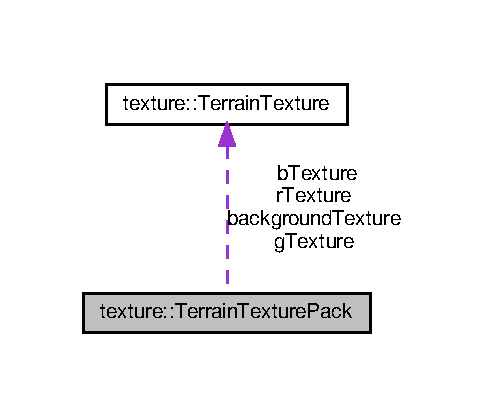
\includegraphics[width=233pt]{classtexture_1_1TerrainTexturePack__coll__graph}
\end{center}
\end{figure}
\subsection*{Javni članovi}
\begin{DoxyCompactItemize}
\item 
\hyperlink{classtexture_1_1TerrainTexturePack_ac10238049352008175e477d2735a0fd6}{Terrain\+Texture\+Pack} (\hyperlink{classtexture_1_1TerrainTexture}{Terrain\+Texture} $\ast$\hyperlink{classtexture_1_1TerrainTexturePack_a5fcc575543662461b66195cfa21875b1}{background\+Texture}, \hyperlink{classtexture_1_1TerrainTexture}{Terrain\+Texture} $\ast$\hyperlink{classtexture_1_1TerrainTexturePack_a08b5f1b7665151358b6b162627fc37d4}{r\+Texture}, \hyperlink{classtexture_1_1TerrainTexture}{Terrain\+Texture} $\ast$\hyperlink{classtexture_1_1TerrainTexturePack_aee84140926644080ce963c6ffe5288da}{g\+Texture}, \hyperlink{classtexture_1_1TerrainTexture}{Terrain\+Texture} $\ast$\hyperlink{classtexture_1_1TerrainTexturePack_a004a654fdda8c9f552f40986e2dd072f}{b\+Texture})
\begin{DoxyCompactList}\small\item\em Konstruktor klase. \end{DoxyCompactList}\item 
\hyperlink{classtexture_1_1TerrainTexturePack_a763a7fb6c053d0998fc17b12adb28c3a}{$\sim$\+Terrain\+Texture\+Pack} ()
\begin{DoxyCompactList}\small\item\em Destruktor klase. \end{DoxyCompactList}\item 
\hyperlink{classtexture_1_1TerrainTexture}{Terrain\+Texture} $\ast$ \hyperlink{classtexture_1_1TerrainTexturePack_afcc4cf5d8e58eb3668cb0bb0e92ac6d9}{get\+Background\+Texture} ()
\begin{DoxyCompactList}\small\item\em Funkcija vraca teksturu pozadine. \end{DoxyCompactList}\item 
\hyperlink{classtexture_1_1TerrainTexture}{Terrain\+Texture} $\ast$ \hyperlink{classtexture_1_1TerrainTexturePack_a2e90d77d35768ae2c2c4a640b354fd2e}{get\+R\+Texture} ()
\begin{DoxyCompactList}\small\item\em Funkcija vraca teksturu odredjenu crvenom bojom. \end{DoxyCompactList}\item 
\hyperlink{classtexture_1_1TerrainTexture}{Terrain\+Texture} $\ast$ \hyperlink{classtexture_1_1TerrainTexturePack_aeaf5b66e3cb399312e265eab07bcdf3f}{get\+G\+Texture} ()
\begin{DoxyCompactList}\small\item\em Funkcija vraca teksturu odredjenu zelenom bojom. \end{DoxyCompactList}\item 
\hyperlink{classtexture_1_1TerrainTexture}{Terrain\+Texture} $\ast$ \hyperlink{classtexture_1_1TerrainTexturePack_a458ca66ed71f945af5e3878de073bb33}{get\+B\+Texture} ()
\begin{DoxyCompactList}\small\item\em Funkcija vraca teksturu odredjenu plavom bojom. \end{DoxyCompactList}\end{DoxyCompactItemize}
\subsection*{Privatni članovi}
\begin{DoxyCompactItemize}
\item 
\hyperlink{classtexture_1_1TerrainTexture}{Terrain\+Texture} $\ast$ \hyperlink{classtexture_1_1TerrainTexturePack_a5fcc575543662461b66195cfa21875b1}{background\+Texture}
\begin{DoxyCompactList}\small\item\em Textura pozadine terena. \end{DoxyCompactList}\item 
\hyperlink{classtexture_1_1TerrainTexture}{Terrain\+Texture} $\ast$ \hyperlink{classtexture_1_1TerrainTexturePack_a08b5f1b7665151358b6b162627fc37d4}{r\+Texture}
\begin{DoxyCompactList}\small\item\em Textura odredjena pozicijom crvene boje. \end{DoxyCompactList}\item 
\hyperlink{classtexture_1_1TerrainTexture}{Terrain\+Texture} $\ast$ \hyperlink{classtexture_1_1TerrainTexturePack_aee84140926644080ce963c6ffe5288da}{g\+Texture}
\begin{DoxyCompactList}\small\item\em Textura odredjena pozicijom zelene boje. \end{DoxyCompactList}\item 
\hyperlink{classtexture_1_1TerrainTexture}{Terrain\+Texture} $\ast$ \hyperlink{classtexture_1_1TerrainTexturePack_a004a654fdda8c9f552f40986e2dd072f}{b\+Texture}
\begin{DoxyCompactList}\small\item\em Textura odredjena pozicijom plave boje. \end{DoxyCompactList}\end{DoxyCompactItemize}


\subsection{Opširniji opis}
Klasa \hyperlink{classtexture_1_1TerrainTexture}{Terrain\+Texture} opisuje sve teksture terena. 

\subsection{Dokumentacija konstruktora i destruktora}
\mbox{\Hypertarget{classtexture_1_1TerrainTexturePack_ac10238049352008175e477d2735a0fd6}\label{classtexture_1_1TerrainTexturePack_ac10238049352008175e477d2735a0fd6}} 
\index{texture\+::\+Terrain\+Texture\+Pack@{texture\+::\+Terrain\+Texture\+Pack}!Terrain\+Texture\+Pack@{Terrain\+Texture\+Pack}}
\index{Terrain\+Texture\+Pack@{Terrain\+Texture\+Pack}!texture\+::\+Terrain\+Texture\+Pack@{texture\+::\+Terrain\+Texture\+Pack}}
\subsubsection{\texorpdfstring{Terrain\+Texture\+Pack()}{TerrainTexturePack()}}
{\footnotesize\ttfamily texture\+::\+Terrain\+Texture\+Pack\+::\+Terrain\+Texture\+Pack (\begin{DoxyParamCaption}\item[{\hyperlink{classtexture_1_1TerrainTexture}{Terrain\+Texture} $\ast$}]{background\+Texture,  }\item[{\hyperlink{classtexture_1_1TerrainTexture}{Terrain\+Texture} $\ast$}]{r\+Texture,  }\item[{\hyperlink{classtexture_1_1TerrainTexture}{Terrain\+Texture} $\ast$}]{g\+Texture,  }\item[{\hyperlink{classtexture_1_1TerrainTexture}{Terrain\+Texture} $\ast$}]{b\+Texture }\end{DoxyParamCaption})}



Konstruktor klase. 


\begin{DoxyParams}{Parametri}
{\em background\+Texture} & Textura pozadine terena. \\
\hline
{\em r\+Texture} & Textura odredjena pozicijom crvene boje. \\
\hline
{\em g\+Texture} & Textura odredjena pozicijom zelene boje. \\
\hline
{\em b\+Texture} & Textura odredjena pozicijom plave boje. \\
\hline
\end{DoxyParams}
\mbox{\Hypertarget{classtexture_1_1TerrainTexturePack_a763a7fb6c053d0998fc17b12adb28c3a}\label{classtexture_1_1TerrainTexturePack_a763a7fb6c053d0998fc17b12adb28c3a}} 
\index{texture\+::\+Terrain\+Texture\+Pack@{texture\+::\+Terrain\+Texture\+Pack}!````~Terrain\+Texture\+Pack@{$\sim$\+Terrain\+Texture\+Pack}}
\index{````~Terrain\+Texture\+Pack@{$\sim$\+Terrain\+Texture\+Pack}!texture\+::\+Terrain\+Texture\+Pack@{texture\+::\+Terrain\+Texture\+Pack}}
\subsubsection{\texorpdfstring{$\sim$\+Terrain\+Texture\+Pack()}{~TerrainTexturePack()}}
{\footnotesize\ttfamily texture\+::\+Terrain\+Texture\+Pack\+::$\sim$\+Terrain\+Texture\+Pack (\begin{DoxyParamCaption}{ }\end{DoxyParamCaption})}



Destruktor klase. 


\begin{DoxyParams}{Parametri}
{\em void} & \\
\hline
\end{DoxyParams}


\subsection{Dokumentacija funkcija članica}
\mbox{\Hypertarget{classtexture_1_1TerrainTexturePack_afcc4cf5d8e58eb3668cb0bb0e92ac6d9}\label{classtexture_1_1TerrainTexturePack_afcc4cf5d8e58eb3668cb0bb0e92ac6d9}} 
\index{texture\+::\+Terrain\+Texture\+Pack@{texture\+::\+Terrain\+Texture\+Pack}!get\+Background\+Texture@{get\+Background\+Texture}}
\index{get\+Background\+Texture@{get\+Background\+Texture}!texture\+::\+Terrain\+Texture\+Pack@{texture\+::\+Terrain\+Texture\+Pack}}
\subsubsection{\texorpdfstring{get\+Background\+Texture()}{getBackgroundTexture()}}
{\footnotesize\ttfamily \hyperlink{classtexture_1_1TerrainTexture}{Terrain\+Texture} $\ast$ texture\+::\+Terrain\+Texture\+Pack\+::get\+Background\+Texture (\begin{DoxyParamCaption}{ }\end{DoxyParamCaption})}



Funkcija vraca teksturu pozadine. 


\begin{DoxyParams}{Parametri}
{\em void} & \\
\hline
\end{DoxyParams}
\begin{DoxyReturn}{Vrednost funkcije}
\hyperlink{classtexture_1_1TerrainTexture}{Terrain\+Texture} $\ast$ Pokazivac na instancu klase \hyperlink{classtexture_1_1TerrainTexture}{Terrain\+Texture}. 
\end{DoxyReturn}
\mbox{\Hypertarget{classtexture_1_1TerrainTexturePack_a458ca66ed71f945af5e3878de073bb33}\label{classtexture_1_1TerrainTexturePack_a458ca66ed71f945af5e3878de073bb33}} 
\index{texture\+::\+Terrain\+Texture\+Pack@{texture\+::\+Terrain\+Texture\+Pack}!get\+B\+Texture@{get\+B\+Texture}}
\index{get\+B\+Texture@{get\+B\+Texture}!texture\+::\+Terrain\+Texture\+Pack@{texture\+::\+Terrain\+Texture\+Pack}}
\subsubsection{\texorpdfstring{get\+B\+Texture()}{getBTexture()}}
{\footnotesize\ttfamily \hyperlink{classtexture_1_1TerrainTexture}{Terrain\+Texture} $\ast$ texture\+::\+Terrain\+Texture\+Pack\+::get\+B\+Texture (\begin{DoxyParamCaption}{ }\end{DoxyParamCaption})}



Funkcija vraca teksturu odredjenu plavom bojom. 


\begin{DoxyParams}{Parametri}
{\em void} & \\
\hline
\end{DoxyParams}
\begin{DoxyReturn}{Vrednost funkcije}
\hyperlink{classtexture_1_1TerrainTexture}{Terrain\+Texture} $\ast$ Pokazivac na instancu klase \hyperlink{classtexture_1_1TerrainTexture}{Terrain\+Texture}. 
\end{DoxyReturn}
\mbox{\Hypertarget{classtexture_1_1TerrainTexturePack_aeaf5b66e3cb399312e265eab07bcdf3f}\label{classtexture_1_1TerrainTexturePack_aeaf5b66e3cb399312e265eab07bcdf3f}} 
\index{texture\+::\+Terrain\+Texture\+Pack@{texture\+::\+Terrain\+Texture\+Pack}!get\+G\+Texture@{get\+G\+Texture}}
\index{get\+G\+Texture@{get\+G\+Texture}!texture\+::\+Terrain\+Texture\+Pack@{texture\+::\+Terrain\+Texture\+Pack}}
\subsubsection{\texorpdfstring{get\+G\+Texture()}{getGTexture()}}
{\footnotesize\ttfamily \hyperlink{classtexture_1_1TerrainTexture}{Terrain\+Texture} $\ast$ texture\+::\+Terrain\+Texture\+Pack\+::get\+G\+Texture (\begin{DoxyParamCaption}{ }\end{DoxyParamCaption})}



Funkcija vraca teksturu odredjenu zelenom bojom. 


\begin{DoxyParams}{Parametri}
{\em void} & \\
\hline
\end{DoxyParams}
\begin{DoxyReturn}{Vrednost funkcije}
\hyperlink{classtexture_1_1TerrainTexture}{Terrain\+Texture} $\ast$ Pokazivac na instancu klase \hyperlink{classtexture_1_1TerrainTexture}{Terrain\+Texture}. 
\end{DoxyReturn}
\mbox{\Hypertarget{classtexture_1_1TerrainTexturePack_a2e90d77d35768ae2c2c4a640b354fd2e}\label{classtexture_1_1TerrainTexturePack_a2e90d77d35768ae2c2c4a640b354fd2e}} 
\index{texture\+::\+Terrain\+Texture\+Pack@{texture\+::\+Terrain\+Texture\+Pack}!get\+R\+Texture@{get\+R\+Texture}}
\index{get\+R\+Texture@{get\+R\+Texture}!texture\+::\+Terrain\+Texture\+Pack@{texture\+::\+Terrain\+Texture\+Pack}}
\subsubsection{\texorpdfstring{get\+R\+Texture()}{getRTexture()}}
{\footnotesize\ttfamily \hyperlink{classtexture_1_1TerrainTexture}{Terrain\+Texture} $\ast$ texture\+::\+Terrain\+Texture\+Pack\+::get\+R\+Texture (\begin{DoxyParamCaption}{ }\end{DoxyParamCaption})}



Funkcija vraca teksturu odredjenu crvenom bojom. 


\begin{DoxyParams}{Parametri}
{\em void} & \\
\hline
\end{DoxyParams}
\begin{DoxyReturn}{Vrednost funkcije}
\hyperlink{classtexture_1_1TerrainTexture}{Terrain\+Texture} $\ast$ Pokazivac na instancu klase \hyperlink{classtexture_1_1TerrainTexture}{Terrain\+Texture}. 
\end{DoxyReturn}


\subsection{Dokumentacija atributa}
\mbox{\Hypertarget{classtexture_1_1TerrainTexturePack_a5fcc575543662461b66195cfa21875b1}\label{classtexture_1_1TerrainTexturePack_a5fcc575543662461b66195cfa21875b1}} 
\index{texture\+::\+Terrain\+Texture\+Pack@{texture\+::\+Terrain\+Texture\+Pack}!background\+Texture@{background\+Texture}}
\index{background\+Texture@{background\+Texture}!texture\+::\+Terrain\+Texture\+Pack@{texture\+::\+Terrain\+Texture\+Pack}}
\subsubsection{\texorpdfstring{background\+Texture}{backgroundTexture}}
{\footnotesize\ttfamily \hyperlink{classtexture_1_1TerrainTexture}{Terrain\+Texture}$\ast$ texture\+::\+Terrain\+Texture\+Pack\+::background\+Texture\hspace{0.3cm}{\ttfamily [private]}}



Textura pozadine terena. 

\mbox{\Hypertarget{classtexture_1_1TerrainTexturePack_a004a654fdda8c9f552f40986e2dd072f}\label{classtexture_1_1TerrainTexturePack_a004a654fdda8c9f552f40986e2dd072f}} 
\index{texture\+::\+Terrain\+Texture\+Pack@{texture\+::\+Terrain\+Texture\+Pack}!b\+Texture@{b\+Texture}}
\index{b\+Texture@{b\+Texture}!texture\+::\+Terrain\+Texture\+Pack@{texture\+::\+Terrain\+Texture\+Pack}}
\subsubsection{\texorpdfstring{b\+Texture}{bTexture}}
{\footnotesize\ttfamily \hyperlink{classtexture_1_1TerrainTexture}{Terrain\+Texture}$\ast$ texture\+::\+Terrain\+Texture\+Pack\+::b\+Texture\hspace{0.3cm}{\ttfamily [private]}}



Textura odredjena pozicijom plave boje. 

\mbox{\Hypertarget{classtexture_1_1TerrainTexturePack_aee84140926644080ce963c6ffe5288da}\label{classtexture_1_1TerrainTexturePack_aee84140926644080ce963c6ffe5288da}} 
\index{texture\+::\+Terrain\+Texture\+Pack@{texture\+::\+Terrain\+Texture\+Pack}!g\+Texture@{g\+Texture}}
\index{g\+Texture@{g\+Texture}!texture\+::\+Terrain\+Texture\+Pack@{texture\+::\+Terrain\+Texture\+Pack}}
\subsubsection{\texorpdfstring{g\+Texture}{gTexture}}
{\footnotesize\ttfamily \hyperlink{classtexture_1_1TerrainTexture}{Terrain\+Texture}$\ast$ texture\+::\+Terrain\+Texture\+Pack\+::g\+Texture\hspace{0.3cm}{\ttfamily [private]}}



Textura odredjena pozicijom zelene boje. 

\mbox{\Hypertarget{classtexture_1_1TerrainTexturePack_a08b5f1b7665151358b6b162627fc37d4}\label{classtexture_1_1TerrainTexturePack_a08b5f1b7665151358b6b162627fc37d4}} 
\index{texture\+::\+Terrain\+Texture\+Pack@{texture\+::\+Terrain\+Texture\+Pack}!r\+Texture@{r\+Texture}}
\index{r\+Texture@{r\+Texture}!texture\+::\+Terrain\+Texture\+Pack@{texture\+::\+Terrain\+Texture\+Pack}}
\subsubsection{\texorpdfstring{r\+Texture}{rTexture}}
{\footnotesize\ttfamily \hyperlink{classtexture_1_1TerrainTexture}{Terrain\+Texture}$\ast$ texture\+::\+Terrain\+Texture\+Pack\+::r\+Texture\hspace{0.3cm}{\ttfamily [private]}}



Textura odredjena pozicijom crvene boje. 



Dokumentacija ove klase je napravljena na osnovu sledećih datoteka\+:\begin{DoxyCompactItemize}
\item 
/home/dusan/\+Documents/\+R\+G146-\/vitez-\/reda-\/zmaja/include/texture/\hyperlink{TerrainTexturePack_8h}{Terrain\+Texture\+Pack.\+h}\item 
/home/dusan/\+Documents/\+R\+G146-\/vitez-\/reda-\/zmaja/src/texture/\hyperlink{TerrainTexturePack_8cpp}{Terrain\+Texture\+Pack.\+cpp}\end{DoxyCompactItemize}

\hypertarget{structtinyobj_1_1texture__option__t}{}\section{Dokumentacija strukture tinyobj\+:\+:texture\+\_\+option\+\_\+t}
\label{structtinyobj_1_1texture__option__t}\index{tinyobj\+::texture\+\_\+option\+\_\+t@{tinyobj\+::texture\+\_\+option\+\_\+t}}


{\ttfamily \#include $<$tiny\+\_\+obj\+\_\+loader.\+h$>$}

\subsection*{Javni članovi}
\begin{DoxyCompactItemize}
\item 
\hyperlink{namespacetinyobj_a5c9f207e1f880a48bac0a3b69f16d7f8}{texture\+\_\+type\+\_\+t} \hyperlink{structtinyobj_1_1texture__option__t_ae93ebf5f70b1b3e3c1de58a257157e00}{type}
\item 
\hyperlink{namespacetinyobj_ad5ca7469ff56bf0d8423120cfd99adce}{real\+\_\+t} \hyperlink{structtinyobj_1_1texture__option__t_a047615e368808b85d5a9cd740ff05846}{sharpness}
\item 
\hyperlink{namespacetinyobj_ad5ca7469ff56bf0d8423120cfd99adce}{real\+\_\+t} \hyperlink{structtinyobj_1_1texture__option__t_a4aea70d3ffbaa6b439db7447557cbab2}{brightness}
\item 
\hyperlink{namespacetinyobj_ad5ca7469ff56bf0d8423120cfd99adce}{real\+\_\+t} \hyperlink{structtinyobj_1_1texture__option__t_a3b81d1c299840825e6633c00ba9ee0e3}{contrast}
\item 
\hyperlink{namespacetinyobj_ad5ca7469ff56bf0d8423120cfd99adce}{real\+\_\+t} \hyperlink{structtinyobj_1_1texture__option__t_ab6a036a11f7b1317709a4d3e25495e07}{origin\+\_\+offset} \mbox{[}3\mbox{]}
\item 
\hyperlink{namespacetinyobj_ad5ca7469ff56bf0d8423120cfd99adce}{real\+\_\+t} \hyperlink{structtinyobj_1_1texture__option__t_a821b861e21a282c14ab702e45ac137dd}{scale} \mbox{[}3\mbox{]}
\item 
\hyperlink{namespacetinyobj_ad5ca7469ff56bf0d8423120cfd99adce}{real\+\_\+t} \hyperlink{structtinyobj_1_1texture__option__t_a39e0e7cb38178022522df240d31709ec}{turbulence} \mbox{[}3\mbox{]}
\item 
bool \hyperlink{structtinyobj_1_1texture__option__t_a55c0ce8fec97910a43606281ea7ee122}{clamp}
\item 
char \hyperlink{structtinyobj_1_1texture__option__t_a2ea1261e85ce71e4f7bacd508a623b65}{imfchan}
\item 
bool \hyperlink{structtinyobj_1_1texture__option__t_a6114c2757e6dd4a4929623797a098d25}{blendu}
\item 
bool \hyperlink{structtinyobj_1_1texture__option__t_a828008c248d350f8d18c04295c773a9c}{blendv}
\item 
\hyperlink{namespacetinyobj_ad5ca7469ff56bf0d8423120cfd99adce}{real\+\_\+t} \hyperlink{structtinyobj_1_1texture__option__t_ad2e2c79e305189e5d146992c32248d49}{bump\+\_\+multiplier}
\end{DoxyCompactItemize}


\subsection{Dokumentacija atributa}
\mbox{\Hypertarget{structtinyobj_1_1texture__option__t_a6114c2757e6dd4a4929623797a098d25}\label{structtinyobj_1_1texture__option__t_a6114c2757e6dd4a4929623797a098d25}} 
\index{tinyobj\+::texture\+\_\+option\+\_\+t@{tinyobj\+::texture\+\_\+option\+\_\+t}!blendu@{blendu}}
\index{blendu@{blendu}!tinyobj\+::texture\+\_\+option\+\_\+t@{tinyobj\+::texture\+\_\+option\+\_\+t}}
\subsubsection{\texorpdfstring{blendu}{blendu}}
{\footnotesize\ttfamily bool tinyobj\+::texture\+\_\+option\+\_\+t\+::blendu}

\mbox{\Hypertarget{structtinyobj_1_1texture__option__t_a828008c248d350f8d18c04295c773a9c}\label{structtinyobj_1_1texture__option__t_a828008c248d350f8d18c04295c773a9c}} 
\index{tinyobj\+::texture\+\_\+option\+\_\+t@{tinyobj\+::texture\+\_\+option\+\_\+t}!blendv@{blendv}}
\index{blendv@{blendv}!tinyobj\+::texture\+\_\+option\+\_\+t@{tinyobj\+::texture\+\_\+option\+\_\+t}}
\subsubsection{\texorpdfstring{blendv}{blendv}}
{\footnotesize\ttfamily bool tinyobj\+::texture\+\_\+option\+\_\+t\+::blendv}

\mbox{\Hypertarget{structtinyobj_1_1texture__option__t_a4aea70d3ffbaa6b439db7447557cbab2}\label{structtinyobj_1_1texture__option__t_a4aea70d3ffbaa6b439db7447557cbab2}} 
\index{tinyobj\+::texture\+\_\+option\+\_\+t@{tinyobj\+::texture\+\_\+option\+\_\+t}!brightness@{brightness}}
\index{brightness@{brightness}!tinyobj\+::texture\+\_\+option\+\_\+t@{tinyobj\+::texture\+\_\+option\+\_\+t}}
\subsubsection{\texorpdfstring{brightness}{brightness}}
{\footnotesize\ttfamily \hyperlink{namespacetinyobj_ad5ca7469ff56bf0d8423120cfd99adce}{real\+\_\+t} tinyobj\+::texture\+\_\+option\+\_\+t\+::brightness}

\mbox{\Hypertarget{structtinyobj_1_1texture__option__t_ad2e2c79e305189e5d146992c32248d49}\label{structtinyobj_1_1texture__option__t_ad2e2c79e305189e5d146992c32248d49}} 
\index{tinyobj\+::texture\+\_\+option\+\_\+t@{tinyobj\+::texture\+\_\+option\+\_\+t}!bump\+\_\+multiplier@{bump\+\_\+multiplier}}
\index{bump\+\_\+multiplier@{bump\+\_\+multiplier}!tinyobj\+::texture\+\_\+option\+\_\+t@{tinyobj\+::texture\+\_\+option\+\_\+t}}
\subsubsection{\texorpdfstring{bump\+\_\+multiplier}{bump\_multiplier}}
{\footnotesize\ttfamily \hyperlink{namespacetinyobj_ad5ca7469ff56bf0d8423120cfd99adce}{real\+\_\+t} tinyobj\+::texture\+\_\+option\+\_\+t\+::bump\+\_\+multiplier}

\mbox{\Hypertarget{structtinyobj_1_1texture__option__t_a55c0ce8fec97910a43606281ea7ee122}\label{structtinyobj_1_1texture__option__t_a55c0ce8fec97910a43606281ea7ee122}} 
\index{tinyobj\+::texture\+\_\+option\+\_\+t@{tinyobj\+::texture\+\_\+option\+\_\+t}!clamp@{clamp}}
\index{clamp@{clamp}!tinyobj\+::texture\+\_\+option\+\_\+t@{tinyobj\+::texture\+\_\+option\+\_\+t}}
\subsubsection{\texorpdfstring{clamp}{clamp}}
{\footnotesize\ttfamily bool tinyobj\+::texture\+\_\+option\+\_\+t\+::clamp}

\mbox{\Hypertarget{structtinyobj_1_1texture__option__t_a3b81d1c299840825e6633c00ba9ee0e3}\label{structtinyobj_1_1texture__option__t_a3b81d1c299840825e6633c00ba9ee0e3}} 
\index{tinyobj\+::texture\+\_\+option\+\_\+t@{tinyobj\+::texture\+\_\+option\+\_\+t}!contrast@{contrast}}
\index{contrast@{contrast}!tinyobj\+::texture\+\_\+option\+\_\+t@{tinyobj\+::texture\+\_\+option\+\_\+t}}
\subsubsection{\texorpdfstring{contrast}{contrast}}
{\footnotesize\ttfamily \hyperlink{namespacetinyobj_ad5ca7469ff56bf0d8423120cfd99adce}{real\+\_\+t} tinyobj\+::texture\+\_\+option\+\_\+t\+::contrast}

\mbox{\Hypertarget{structtinyobj_1_1texture__option__t_a2ea1261e85ce71e4f7bacd508a623b65}\label{structtinyobj_1_1texture__option__t_a2ea1261e85ce71e4f7bacd508a623b65}} 
\index{tinyobj\+::texture\+\_\+option\+\_\+t@{tinyobj\+::texture\+\_\+option\+\_\+t}!imfchan@{imfchan}}
\index{imfchan@{imfchan}!tinyobj\+::texture\+\_\+option\+\_\+t@{tinyobj\+::texture\+\_\+option\+\_\+t}}
\subsubsection{\texorpdfstring{imfchan}{imfchan}}
{\footnotesize\ttfamily char tinyobj\+::texture\+\_\+option\+\_\+t\+::imfchan}

\mbox{\Hypertarget{structtinyobj_1_1texture__option__t_ab6a036a11f7b1317709a4d3e25495e07}\label{structtinyobj_1_1texture__option__t_ab6a036a11f7b1317709a4d3e25495e07}} 
\index{tinyobj\+::texture\+\_\+option\+\_\+t@{tinyobj\+::texture\+\_\+option\+\_\+t}!origin\+\_\+offset@{origin\+\_\+offset}}
\index{origin\+\_\+offset@{origin\+\_\+offset}!tinyobj\+::texture\+\_\+option\+\_\+t@{tinyobj\+::texture\+\_\+option\+\_\+t}}
\subsubsection{\texorpdfstring{origin\+\_\+offset}{origin\_offset}}
{\footnotesize\ttfamily \hyperlink{namespacetinyobj_ad5ca7469ff56bf0d8423120cfd99adce}{real\+\_\+t} tinyobj\+::texture\+\_\+option\+\_\+t\+::origin\+\_\+offset\mbox{[}3\mbox{]}}

\mbox{\Hypertarget{structtinyobj_1_1texture__option__t_a821b861e21a282c14ab702e45ac137dd}\label{structtinyobj_1_1texture__option__t_a821b861e21a282c14ab702e45ac137dd}} 
\index{tinyobj\+::texture\+\_\+option\+\_\+t@{tinyobj\+::texture\+\_\+option\+\_\+t}!scale@{scale}}
\index{scale@{scale}!tinyobj\+::texture\+\_\+option\+\_\+t@{tinyobj\+::texture\+\_\+option\+\_\+t}}
\subsubsection{\texorpdfstring{scale}{scale}}
{\footnotesize\ttfamily \hyperlink{namespacetinyobj_ad5ca7469ff56bf0d8423120cfd99adce}{real\+\_\+t} tinyobj\+::texture\+\_\+option\+\_\+t\+::scale\mbox{[}3\mbox{]}}

\mbox{\Hypertarget{structtinyobj_1_1texture__option__t_a047615e368808b85d5a9cd740ff05846}\label{structtinyobj_1_1texture__option__t_a047615e368808b85d5a9cd740ff05846}} 
\index{tinyobj\+::texture\+\_\+option\+\_\+t@{tinyobj\+::texture\+\_\+option\+\_\+t}!sharpness@{sharpness}}
\index{sharpness@{sharpness}!tinyobj\+::texture\+\_\+option\+\_\+t@{tinyobj\+::texture\+\_\+option\+\_\+t}}
\subsubsection{\texorpdfstring{sharpness}{sharpness}}
{\footnotesize\ttfamily \hyperlink{namespacetinyobj_ad5ca7469ff56bf0d8423120cfd99adce}{real\+\_\+t} tinyobj\+::texture\+\_\+option\+\_\+t\+::sharpness}

\mbox{\Hypertarget{structtinyobj_1_1texture__option__t_a39e0e7cb38178022522df240d31709ec}\label{structtinyobj_1_1texture__option__t_a39e0e7cb38178022522df240d31709ec}} 
\index{tinyobj\+::texture\+\_\+option\+\_\+t@{tinyobj\+::texture\+\_\+option\+\_\+t}!turbulence@{turbulence}}
\index{turbulence@{turbulence}!tinyobj\+::texture\+\_\+option\+\_\+t@{tinyobj\+::texture\+\_\+option\+\_\+t}}
\subsubsection{\texorpdfstring{turbulence}{turbulence}}
{\footnotesize\ttfamily \hyperlink{namespacetinyobj_ad5ca7469ff56bf0d8423120cfd99adce}{real\+\_\+t} tinyobj\+::texture\+\_\+option\+\_\+t\+::turbulence\mbox{[}3\mbox{]}}

\mbox{\Hypertarget{structtinyobj_1_1texture__option__t_ae93ebf5f70b1b3e3c1de58a257157e00}\label{structtinyobj_1_1texture__option__t_ae93ebf5f70b1b3e3c1de58a257157e00}} 
\index{tinyobj\+::texture\+\_\+option\+\_\+t@{tinyobj\+::texture\+\_\+option\+\_\+t}!type@{type}}
\index{type@{type}!tinyobj\+::texture\+\_\+option\+\_\+t@{tinyobj\+::texture\+\_\+option\+\_\+t}}
\subsubsection{\texorpdfstring{type}{type}}
{\footnotesize\ttfamily \hyperlink{namespacetinyobj_a5c9f207e1f880a48bac0a3b69f16d7f8}{texture\+\_\+type\+\_\+t} tinyobj\+::texture\+\_\+option\+\_\+t\+::type}



Dokumentacija ove strukture je napravljena na osnovu datoteke \begin{DoxyCompactItemize}
\item 
/home/dusan/\+Documents/\+R\+G146-\/vitez-\/reda-\/zmaja/include/external\+\_\+libs/\hyperlink{tiny__obj__loader_8h}{tiny\+\_\+obj\+\_\+loader.\+h}\end{DoxyCompactItemize}

\hypertarget{classmodel_1_1TexturedModel}{}\section{Dokumentacija klase model\+:\+:Textured\+Model}
\label{classmodel_1_1TexturedModel}\index{model\+::\+Textured\+Model@{model\+::\+Textured\+Model}}


Klasa \hyperlink{classmodel_1_1TexturedModel}{Textured\+Model} opisuje model objekta zajedno sa teksturom. Model je opisan instancom klase \hyperlink{classmodel_1_1RawModel}{Raw\+Model} i odgovarajucom teksturom objekta pomocu instance klase Model\+Texture.  




{\ttfamily \#include $<$Textured\+Model.\+h$>$}



Klasni dijagram za model\+:\+:Textured\+Model\+:\nopagebreak
\begin{figure}[H]
\begin{center}
\leavevmode
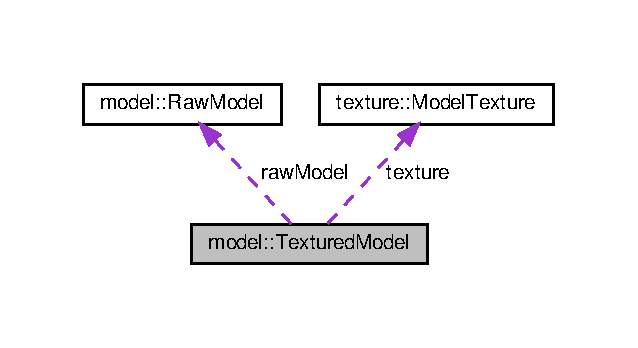
\includegraphics[width=306pt]{classmodel_1_1TexturedModel__coll__graph}
\end{center}
\end{figure}
\subsection*{Javni članovi}
\begin{DoxyCompactItemize}
\item 
\hyperlink{classmodel_1_1TexturedModel_affbb36dc66a365064576e186a975777a}{Textured\+Model} (\hyperlink{classmodel_1_1RawModel}{Raw\+Model} $\ast$model, \hyperlink{classtexture_1_1ModelTexture}{Model\+Texture} $\ast$\hyperlink{classmodel_1_1TexturedModel_aad9aacee1ff02e44bd8ee9daff22f817}{texture})
\begin{DoxyCompactList}\small\item\em Konstruktor klase. U konstruktoru se modelu pridruzuju neteksturisani objekat i njegova tekstura. \end{DoxyCompactList}\item 
\hyperlink{classmodel_1_1TexturedModel_a8a11ba96d5a73a962a2ffcf8c5a53afe}{$\sim$\+Textured\+Model} ()
\begin{DoxyCompactList}\small\item\em Destruktor klase. \end{DoxyCompactList}\item 
\hyperlink{classmodel_1_1RawModel}{Raw\+Model} \hyperlink{classmodel_1_1TexturedModel_a8074adea6d7e368690a977b4ad571378}{get\+Raw\+Model} (void)
\begin{DoxyCompactList}\small\item\em Funkcija vraca osnovni model objekta. \end{DoxyCompactList}\item 
\hyperlink{classtexture_1_1ModelTexture}{Model\+Texture} $\ast$ \hyperlink{classmodel_1_1TexturedModel_ad2bb5d174a506bd9d1f807e84aba4cdc}{get\+Texture} (void)
\begin{DoxyCompactList}\small\item\em Funkcija vraca teksturu modela. \end{DoxyCompactList}\end{DoxyCompactItemize}
\subsection*{Privatni članovi}
\begin{DoxyCompactItemize}
\item 
\hyperlink{classmodel_1_1RawModel}{Raw\+Model} $\ast$ \hyperlink{classmodel_1_1TexturedModel_ac6157368c7e55a78aa02f9546f5f2dc3}{raw\+Model}
\begin{DoxyCompactList}\small\item\em Pokazivac na model objekta bez pridruzene strukture. \end{DoxyCompactList}\item 
\hyperlink{classtexture_1_1ModelTexture}{Model\+Texture} $\ast$ \hyperlink{classmodel_1_1TexturedModel_aad9aacee1ff02e44bd8ee9daff22f817}{texture}
\begin{DoxyCompactList}\small\item\em Pokazivac na teksturu objekta. \end{DoxyCompactList}\end{DoxyCompactItemize}


\subsection{Opširniji opis}
Klasa \hyperlink{classmodel_1_1TexturedModel}{Textured\+Model} opisuje model objekta zajedno sa teksturom. Model je opisan instancom klase \hyperlink{classmodel_1_1RawModel}{Raw\+Model} i odgovarajucom teksturom objekta pomocu instance klase Model\+Texture. 

\subsection{Dokumentacija konstruktora i destruktora}
\mbox{\Hypertarget{classmodel_1_1TexturedModel_affbb36dc66a365064576e186a975777a}\label{classmodel_1_1TexturedModel_affbb36dc66a365064576e186a975777a}} 
\index{model\+::\+Textured\+Model@{model\+::\+Textured\+Model}!Textured\+Model@{Textured\+Model}}
\index{Textured\+Model@{Textured\+Model}!model\+::\+Textured\+Model@{model\+::\+Textured\+Model}}
\subsubsection{\texorpdfstring{Textured\+Model()}{TexturedModel()}}
{\footnotesize\ttfamily model\+::\+Textured\+Model\+::\+Textured\+Model (\begin{DoxyParamCaption}\item[{\hyperlink{classmodel_1_1RawModel}{Raw\+Model} $\ast$}]{model,  }\item[{\hyperlink{classtexture_1_1ModelTexture}{Model\+Texture} $\ast$}]{texture }\end{DoxyParamCaption})}



Konstruktor klase. U konstruktoru se modelu pridruzuju neteksturisani objekat i njegova tekstura. 


\begin{DoxyParams}{Parametri}
{\em model} & Pokazivac na model objekta bez pridruzene strukture. \\
\hline
{\em texture} & Pokazivac na teksturu objekta. \\
\hline
\end{DoxyParams}
\mbox{\Hypertarget{classmodel_1_1TexturedModel_a8a11ba96d5a73a962a2ffcf8c5a53afe}\label{classmodel_1_1TexturedModel_a8a11ba96d5a73a962a2ffcf8c5a53afe}} 
\index{model\+::\+Textured\+Model@{model\+::\+Textured\+Model}!````~Textured\+Model@{$\sim$\+Textured\+Model}}
\index{````~Textured\+Model@{$\sim$\+Textured\+Model}!model\+::\+Textured\+Model@{model\+::\+Textured\+Model}}
\subsubsection{\texorpdfstring{$\sim$\+Textured\+Model()}{~TexturedModel()}}
{\footnotesize\ttfamily model\+::\+Textured\+Model\+::$\sim$\+Textured\+Model (\begin{DoxyParamCaption}{ }\end{DoxyParamCaption})}



Destruktor klase. 


\begin{DoxyParams}{Parametri}
{\em void} & \\
\hline
\end{DoxyParams}


\subsection{Dokumentacija funkcija članica}
\mbox{\Hypertarget{classmodel_1_1TexturedModel_a8074adea6d7e368690a977b4ad571378}\label{classmodel_1_1TexturedModel_a8074adea6d7e368690a977b4ad571378}} 
\index{model\+::\+Textured\+Model@{model\+::\+Textured\+Model}!get\+Raw\+Model@{get\+Raw\+Model}}
\index{get\+Raw\+Model@{get\+Raw\+Model}!model\+::\+Textured\+Model@{model\+::\+Textured\+Model}}
\subsubsection{\texorpdfstring{get\+Raw\+Model()}{getRawModel()}}
{\footnotesize\ttfamily \hyperlink{classmodel_1_1RawModel}{Raw\+Model} model\+::\+Textured\+Model\+::get\+Raw\+Model (\begin{DoxyParamCaption}\item[{void}]{ }\end{DoxyParamCaption})}



Funkcija vraca osnovni model objekta. 


\begin{DoxyParams}{Parametri}
{\em void} & \\
\hline
\end{DoxyParams}
\begin{DoxyReturn}{Vrednost funkcije}
\hyperlink{classmodel_1_1RawModel}{Raw\+Model} Osnovni model objekta. 
\end{DoxyReturn}
\mbox{\Hypertarget{classmodel_1_1TexturedModel_ad2bb5d174a506bd9d1f807e84aba4cdc}\label{classmodel_1_1TexturedModel_ad2bb5d174a506bd9d1f807e84aba4cdc}} 
\index{model\+::\+Textured\+Model@{model\+::\+Textured\+Model}!get\+Texture@{get\+Texture}}
\index{get\+Texture@{get\+Texture}!model\+::\+Textured\+Model@{model\+::\+Textured\+Model}}
\subsubsection{\texorpdfstring{get\+Texture()}{getTexture()}}
{\footnotesize\ttfamily \hyperlink{classtexture_1_1ModelTexture}{Model\+Texture} $\ast$ model\+::\+Textured\+Model\+::get\+Texture (\begin{DoxyParamCaption}\item[{void}]{ }\end{DoxyParamCaption})}



Funkcija vraca teksturu modela. 


\begin{DoxyParams}{Parametri}
{\em void} & \\
\hline
\end{DoxyParams}
\begin{DoxyReturn}{Vrednost funkcije}
Model\+Texture Tekstura modela. 
\end{DoxyReturn}


\subsection{Dokumentacija atributa}
\mbox{\Hypertarget{classmodel_1_1TexturedModel_ac6157368c7e55a78aa02f9546f5f2dc3}\label{classmodel_1_1TexturedModel_ac6157368c7e55a78aa02f9546f5f2dc3}} 
\index{model\+::\+Textured\+Model@{model\+::\+Textured\+Model}!raw\+Model@{raw\+Model}}
\index{raw\+Model@{raw\+Model}!model\+::\+Textured\+Model@{model\+::\+Textured\+Model}}
\subsubsection{\texorpdfstring{raw\+Model}{rawModel}}
{\footnotesize\ttfamily \hyperlink{classmodel_1_1RawModel}{Raw\+Model}$\ast$ model\+::\+Textured\+Model\+::raw\+Model\hspace{0.3cm}{\ttfamily [private]}}



Pokazivac na model objekta bez pridruzene strukture. 

\mbox{\Hypertarget{classmodel_1_1TexturedModel_aad9aacee1ff02e44bd8ee9daff22f817}\label{classmodel_1_1TexturedModel_aad9aacee1ff02e44bd8ee9daff22f817}} 
\index{model\+::\+Textured\+Model@{model\+::\+Textured\+Model}!texture@{texture}}
\index{texture@{texture}!model\+::\+Textured\+Model@{model\+::\+Textured\+Model}}
\subsubsection{\texorpdfstring{texture}{texture}}
{\footnotesize\ttfamily \hyperlink{classtexture_1_1ModelTexture}{Model\+Texture}$\ast$ model\+::\+Textured\+Model\+::texture\hspace{0.3cm}{\ttfamily [private]}}



Pokazivac na teksturu objekta. 



Dokumentacija ove klase je napravljena na osnovu sledećih datoteka\+:\begin{DoxyCompactItemize}
\item 
/home/dusan/\+Documents/\+R\+G146-\/vitez-\/reda-\/zmaja/include/model/\hyperlink{TexturedModel_8h}{Textured\+Model.\+h}\item 
/home/dusan/\+Documents/\+R\+G146-\/vitez-\/reda-\/zmaja/src/model/\hyperlink{TexturedModel_8cpp}{Textured\+Model.\+cpp}\end{DoxyCompactItemize}

\hypertarget{classcore_1_1VaoLoader}{}\section{Dokumentacija klase core\+:\+:Vao\+Loader}
\label{classcore_1_1VaoLoader}\index{core\+::\+Vao\+Loader@{core\+::\+Vao\+Loader}}


Klasa \hyperlink{classcore_1_1VaoLoader}{Vao\+Loader} je zaduzena za ucitavanje atributa u memoriju. Zadatak ove klase je ucitavanje i definisanje objekta pomocu niza atributa gde se svaki atribut ucitava u baffer koji je niz promenljivih. Ovo dovodi do komplikovanijeg koda ali kod je genericki i pomocu njega mozemo ucitavati veoma slozene objekte i texture sto bi bilo vrlo tesko kada bi smo svaki objekat sami crtali osnovnim Open\+GL funkcijama.  




{\ttfamily \#include $<$Vao\+Loader.\+h$>$}

\subsection*{Javni članovi}
\begin{DoxyCompactItemize}
\item 
\hyperlink{classcore_1_1VaoLoader_ab025be7312c274b9737b19d308bd5845}{Vao\+Loader} ()
\begin{DoxyCompactList}\small\item\em Konstruktor klase. \end{DoxyCompactList}\item 
\hyperlink{classcore_1_1VaoLoader_a1b522bb4b83dbe751783fee04ac712d3}{$\sim$\+Vao\+Loader} ()
\begin{DoxyCompactList}\small\item\em Destruktor klase. \end{DoxyCompactList}\item 
G\+Lint \hyperlink{classcore_1_1VaoLoader_a66f6bd69acb88c9eb8ff73353d3b5312}{load\+To\+Vao} (G\+Lfloat positions\mbox{[}$\,$\mbox{]}, G\+Lint positions\+Size, G\+Lint indices\mbox{[}$\,$\mbox{]}, G\+Lint indices\+Size, G\+Lfloat texture\+Coords\mbox{[}$\,$\mbox{]}, G\+Lint texture\+Size, G\+Lfloat normals\mbox{[}$\,$\mbox{]}, G\+Lint normals\+Size)
\begin{DoxyCompactList}\small\item\em Funkcija kreira niz atributa(\+V\+A\+O). U funkciji se prvo kreira vao i dodeljuje mu se identifikator nakon cega se parametri funkcije ucitavaju u bafere koji se pridruzuju ranije kreiranom vao-\/u. \end{DoxyCompactList}\item 
G\+Lint \hyperlink{classcore_1_1VaoLoader_afca30e4e6537fbc3c03c24f3eb46cfad}{load\+To\+Vao} (G\+Lfloat positions\mbox{[}$\,$\mbox{]}, G\+Lint positions\+Size, G\+Lint indices\mbox{[}$\,$\mbox{]}, G\+Lint indices\+Size, G\+Lfloat texture\+Coords\mbox{[}$\,$\mbox{]}, G\+Lint texture\+Size, G\+Lfloat normals\mbox{[}$\,$\mbox{]}, G\+Lint normals\+Size, G\+Lint bone\+Indices\mbox{[}$\,$\mbox{]}, G\+Lint bone\+Indices\+Size, G\+Lfloat weights\mbox{[}$\,$\mbox{]}, G\+Lint weights\+Size)
\begin{DoxyCompactList}\small\item\em Funkcija kreira niz atributa(\+V\+A\+O). U funkciji se prvo kreira vao i dodeljuje mu se identifikator nakon cega se parametri funkcije ucitavaju u bafere koji se pridruzuju ranije kreiranom vao-\/u. \end{DoxyCompactList}\item 
G\+Lint \hyperlink{classcore_1_1VaoLoader_aebc9e5741cb2458b06859aad21621e08}{load\+To\+Vao} (G\+Lfloat positions\mbox{[}$\,$\mbox{]}, G\+Lint positions\+Size, int dimensions)
\begin{DoxyCompactList}\small\item\em Funkcija kreira niz atributa(\+V\+A\+O). U funkciji se prvo kreira vao i dodeljuje mu se identifikator nakon cega se parametri funkcije ucitavaju u bafere koji se pridruzuju ranije kreiranom vao-\/u. \end{DoxyCompactList}\item 
G\+Lint \hyperlink{classcore_1_1VaoLoader_aeefd4de3346c1036d8d7249694fd404d}{load\+Texture} (const char $\ast$file\+Name)
\begin{DoxyCompactList}\small\item\em Funkcija ucitava texturu iz png fajla. U funkciji se pomocu png biblioteke citaju informacije iz fajla koje se zatim upisuju u Open\+GL teksturu sa kreiranim identifikatorom. \end{DoxyCompactList}\item 
G\+Luint \hyperlink{classcore_1_1VaoLoader_a98165161bee2940808fe5e546dfa25d9}{load\+Cube\+Map} (vector$<$ const char $\ast$$>$ texture\+Files)
\begin{DoxyCompactList}\small\item\em Funkcija ucitava texture u kubnu mapu. \end{DoxyCompactList}\item 
void \hyperlink{classcore_1_1VaoLoader_a15a5ec23ffe560ad7117980aaf0d97b9}{clean\+Up} (void)
\begin{DoxyCompactList}\small\item\em Funkcija brise podatke iz memorije. U funkciji se prethodno kreirani identifikatori brisu zajedno sa informacijama koje identifikuju. \end{DoxyCompactList}\end{DoxyCompactItemize}
\subsection*{Privatni članovi}
\begin{DoxyCompactItemize}
\item 
int \hyperlink{classcore_1_1VaoLoader_af76598a15d38378e594778d9a63a7a6a}{create\+Vao} (void)
\begin{DoxyCompactList}\small\item\em Funkcija kreira niz atributa(\+V\+A\+O). \end{DoxyCompactList}\item 
void \hyperlink{classcore_1_1VaoLoader_a234b87947a46ffcaea7dc6de09185a41}{store\+Data\+In\+Vertex\+Buffer} (G\+Lint attribute\+Number, int coordinate\+Size, G\+Lfloat data\mbox{[}$\,$\mbox{]}, G\+Lint data\+Size)
\begin{DoxyCompactList}\small\item\em Funkcija startuje bitne procese za funkcionisanje. U funkciji se kreira bafer u koji se smestaju informacije vazane za objekat. \end{DoxyCompactList}\item 
void \hyperlink{classcore_1_1VaoLoader_a4e9c5aee112aa6194ea776bc7eeaf98f}{store\+Data\+In\+Vertex\+Buffer} (G\+Lint attribute\+Number, int coordinate\+Size, G\+Lint data\mbox{[}$\,$\mbox{]}, G\+Lint data\+Size)
\begin{DoxyCompactList}\small\item\em Funkcija startuje bitne procese za funkcionisanje. U funkciji se kreira bafer u koji se smestaju informacije vazane za objekat. \end{DoxyCompactList}\item 
void \hyperlink{classcore_1_1VaoLoader_a7195d251490976b2053548e19b7c6f1d}{store\+Data\+In\+Indices\+Buffer} (G\+Lint data\mbox{[}$\,$\mbox{]}, G\+Lint data\+Size)
\begin{DoxyCompactList}\small\item\em Funkcija ucitava indekse tacaka. U funkciji se kreira bafer u koji se smestaju indeksi tacaka objekta. \end{DoxyCompactList}\item 
void \hyperlink{classcore_1_1VaoLoader_a8876e8e71b0299c47406afc7a2cb6d81}{unbind\+Vao} (void)
\begin{DoxyCompactList}\small\item\em Funkcija prekida vezu sa nizom atributa. \end{DoxyCompactList}\item 
vector$<$ float $>$ \hyperlink{classcore_1_1VaoLoader_a016f118749e83bbf79e6d0f2c9bf9209}{store\+Data\+In\+Float\+Buffer} (G\+Lfloat data\mbox{[}$\,$\mbox{]}, G\+Lint data\+Size)
\begin{DoxyCompactList}\small\item\em Funkcija ucitava niz u bafer podataka. U funkciji se podaci iz niza ucitavaju u bafer realnih brojeva zbog kasnijeg ucitavanja pomocu Open\+GL funkcija. \end{DoxyCompactList}\item 
vector$<$ int $>$ \hyperlink{classcore_1_1VaoLoader_ab2c24b482be973465c548b03bf5df3af}{store\+Data\+In\+Int\+Buffer} (G\+Lint data\mbox{[}$\,$\mbox{]}, G\+Lint data\+Size)
\begin{DoxyCompactList}\small\item\em Funkcija ucitava niz u bafer podataka. U funkciji se podaci iz niza ucitavaju u bafer celih brojeva zbog kasnijeg ucitavanja pomocu Open\+GL funkcija. \end{DoxyCompactList}\item 
\hyperlink{classtexture_1_1SkyboxTextureData}{Skybox\+Texture\+Data} $\ast$ \hyperlink{classcore_1_1VaoLoader_a8310742834449c159828f87e771a5258}{decode\+Texture\+File} (const char $\ast$file\+Name)
\begin{DoxyCompactList}\small\item\em Funkcija cita podatke iz fajla teksture. \end{DoxyCompactList}\end{DoxyCompactItemize}
\subsection*{Privatni članovi}
\begin{DoxyCompactItemize}
\item 
G\+Luint \hyperlink{classcore_1_1VaoLoader_a09fec3fcaf674c66046a859e60c9c674}{vao\+ID}
\begin{DoxyCompactList}\small\item\em Identifikator niza atributa. \end{DoxyCompactList}\item 
G\+Luint \hyperlink{classcore_1_1VaoLoader_a4bc8031f15ad1b7c7eff491f926b93e4}{vbo\+ID}
\begin{DoxyCompactList}\small\item\em Identifikator bafera koji postaje clan niza atributa. \end{DoxyCompactList}\item 
vector$<$ G\+Luint $>$ \hyperlink{classcore_1_1VaoLoader_ad37e6f10d175e35a6fce4b9f76b559e2}{vaos}
\begin{DoxyCompactList}\small\item\em Niz svih identifikatora niza atributa. \end{DoxyCompactList}\item 
vector$<$ G\+Luint $>$ \hyperlink{classcore_1_1VaoLoader_a8866245dbda8794e13956115557159a2}{vbos}
\begin{DoxyCompactList}\small\item\em Niz svih identifikatora bafera. \end{DoxyCompactList}\item 
vector$<$ G\+Lint $>$ \hyperlink{classcore_1_1VaoLoader_a6f2a03c0bca3b9c8211215014747cbaa}{textures}
\begin{DoxyCompactList}\small\item\em Niz svih identifikatora tekstura. \end{DoxyCompactList}\end{DoxyCompactItemize}


\subsection{Opširniji opis}
Klasa \hyperlink{classcore_1_1VaoLoader}{Vao\+Loader} je zaduzena za ucitavanje atributa u memoriju. Zadatak ove klase je ucitavanje i definisanje objekta pomocu niza atributa gde se svaki atribut ucitava u baffer koji je niz promenljivih. Ovo dovodi do komplikovanijeg koda ali kod je genericki i pomocu njega mozemo ucitavati veoma slozene objekte i texture sto bi bilo vrlo tesko kada bi smo svaki objekat sami crtali osnovnim Open\+GL funkcijama. 

\subsection{Dokumentacija konstruktora i destruktora}
\mbox{\Hypertarget{classcore_1_1VaoLoader_ab025be7312c274b9737b19d308bd5845}\label{classcore_1_1VaoLoader_ab025be7312c274b9737b19d308bd5845}} 
\index{core\+::\+Vao\+Loader@{core\+::\+Vao\+Loader}!Vao\+Loader@{Vao\+Loader}}
\index{Vao\+Loader@{Vao\+Loader}!core\+::\+Vao\+Loader@{core\+::\+Vao\+Loader}}
\subsubsection{\texorpdfstring{Vao\+Loader()}{VaoLoader()}}
{\footnotesize\ttfamily core\+::\+Vao\+Loader\+::\+Vao\+Loader (\begin{DoxyParamCaption}{ }\end{DoxyParamCaption})}



Konstruktor klase. 


\begin{DoxyParams}{Parametri}
{\em void} & \\
\hline
\end{DoxyParams}
\mbox{\Hypertarget{classcore_1_1VaoLoader_a1b522bb4b83dbe751783fee04ac712d3}\label{classcore_1_1VaoLoader_a1b522bb4b83dbe751783fee04ac712d3}} 
\index{core\+::\+Vao\+Loader@{core\+::\+Vao\+Loader}!````~Vao\+Loader@{$\sim$\+Vao\+Loader}}
\index{````~Vao\+Loader@{$\sim$\+Vao\+Loader}!core\+::\+Vao\+Loader@{core\+::\+Vao\+Loader}}
\subsubsection{\texorpdfstring{$\sim$\+Vao\+Loader()}{~VaoLoader()}}
{\footnotesize\ttfamily core\+::\+Vao\+Loader\+::$\sim$\+Vao\+Loader (\begin{DoxyParamCaption}{ }\end{DoxyParamCaption})}



Destruktor klase. 


\begin{DoxyParams}{Parametri}
{\em void} & \\
\hline
\end{DoxyParams}


\subsection{Dokumentacija funkcija članica}
\mbox{\Hypertarget{classcore_1_1VaoLoader_a15a5ec23ffe560ad7117980aaf0d97b9}\label{classcore_1_1VaoLoader_a15a5ec23ffe560ad7117980aaf0d97b9}} 
\index{core\+::\+Vao\+Loader@{core\+::\+Vao\+Loader}!clean\+Up@{clean\+Up}}
\index{clean\+Up@{clean\+Up}!core\+::\+Vao\+Loader@{core\+::\+Vao\+Loader}}
\subsubsection{\texorpdfstring{clean\+Up()}{cleanUp()}}
{\footnotesize\ttfamily void core\+::\+Vao\+Loader\+::clean\+Up (\begin{DoxyParamCaption}\item[{void}]{ }\end{DoxyParamCaption})}



Funkcija brise podatke iz memorije. U funkciji se prethodno kreirani identifikatori brisu zajedno sa informacijama koje identifikuju. 


\begin{DoxyParams}{Parametri}
{\em void} & \\
\hline
\end{DoxyParams}
\begin{DoxyReturn}{Vrednost funkcije}
void 
\end{DoxyReturn}
\mbox{\Hypertarget{classcore_1_1VaoLoader_af76598a15d38378e594778d9a63a7a6a}\label{classcore_1_1VaoLoader_af76598a15d38378e594778d9a63a7a6a}} 
\index{core\+::\+Vao\+Loader@{core\+::\+Vao\+Loader}!create\+Vao@{create\+Vao}}
\index{create\+Vao@{create\+Vao}!core\+::\+Vao\+Loader@{core\+::\+Vao\+Loader}}
\subsubsection{\texorpdfstring{create\+Vao()}{createVao()}}
{\footnotesize\ttfamily int core\+::\+Vao\+Loader\+::create\+Vao (\begin{DoxyParamCaption}\item[{void}]{ }\end{DoxyParamCaption})\hspace{0.3cm}{\ttfamily [private]}}



Funkcija kreira niz atributa(\+V\+A\+O). 


\begin{DoxyParams}{Parametri}
{\em void} & \\
\hline
\end{DoxyParams}
\begin{DoxyReturn}{Vrednost funkcije}
int Identifikator kreiranog niza atributa. 
\end{DoxyReturn}
\mbox{\Hypertarget{classcore_1_1VaoLoader_a8310742834449c159828f87e771a5258}\label{classcore_1_1VaoLoader_a8310742834449c159828f87e771a5258}} 
\index{core\+::\+Vao\+Loader@{core\+::\+Vao\+Loader}!decode\+Texture\+File@{decode\+Texture\+File}}
\index{decode\+Texture\+File@{decode\+Texture\+File}!core\+::\+Vao\+Loader@{core\+::\+Vao\+Loader}}
\subsubsection{\texorpdfstring{decode\+Texture\+File()}{decodeTextureFile()}}
{\footnotesize\ttfamily \hyperlink{classtexture_1_1SkyboxTextureData}{Skybox\+Texture\+Data} $\ast$ core\+::\+Vao\+Loader\+::decode\+Texture\+File (\begin{DoxyParamCaption}\item[{const char $\ast$}]{file\+Name }\end{DoxyParamCaption})\hspace{0.3cm}{\ttfamily [private]}}



Funkcija cita podatke iz fajla teksture. 


\begin{DoxyParams}{Parametri}
{\em file\+Name} & Naziv fajla teksture. \\
\hline
\end{DoxyParams}
\begin{DoxyReturn}{Vrednost funkcije}
Skybox\+Texture\+Data$\ast$ Pokazivac na instancu klase Skybox\+Texture\+Data 
\end{DoxyReturn}
\mbox{\Hypertarget{classcore_1_1VaoLoader_a98165161bee2940808fe5e546dfa25d9}\label{classcore_1_1VaoLoader_a98165161bee2940808fe5e546dfa25d9}} 
\index{core\+::\+Vao\+Loader@{core\+::\+Vao\+Loader}!load\+Cube\+Map@{load\+Cube\+Map}}
\index{load\+Cube\+Map@{load\+Cube\+Map}!core\+::\+Vao\+Loader@{core\+::\+Vao\+Loader}}
\subsubsection{\texorpdfstring{load\+Cube\+Map()}{loadCubeMap()}}
{\footnotesize\ttfamily G\+Luint core\+::\+Vao\+Loader\+::load\+Cube\+Map (\begin{DoxyParamCaption}\item[{vector$<$ const char $\ast$$>$}]{texture\+Files }\end{DoxyParamCaption})}



Funkcija ucitava texture u kubnu mapu. 


\begin{DoxyParams}{Parametri}
{\em texture\+Files} & Niz imena tekstura; \\
\hline
\end{DoxyParams}
\begin{DoxyReturn}{Vrednost funkcije}
G\+Luint Identifikarot kubne mape tekstura. 
\end{DoxyReturn}
\mbox{\Hypertarget{classcore_1_1VaoLoader_aeefd4de3346c1036d8d7249694fd404d}\label{classcore_1_1VaoLoader_aeefd4de3346c1036d8d7249694fd404d}} 
\index{core\+::\+Vao\+Loader@{core\+::\+Vao\+Loader}!load\+Texture@{load\+Texture}}
\index{load\+Texture@{load\+Texture}!core\+::\+Vao\+Loader@{core\+::\+Vao\+Loader}}
\subsubsection{\texorpdfstring{load\+Texture()}{loadTexture()}}
{\footnotesize\ttfamily int core\+::\+Vao\+Loader\+::load\+Texture (\begin{DoxyParamCaption}\item[{const char $\ast$}]{file\+Name }\end{DoxyParamCaption})}



Funkcija ucitava texturu iz png fajla. U funkciji se pomocu png biblioteke citaju informacije iz fajla koje se zatim upisuju u Open\+GL teksturu sa kreiranim identifikatorom. 


\begin{DoxyParams}{Parametri}
{\em file\+Name} & Ime png fajla. \\
\hline
\end{DoxyParams}
\begin{DoxyReturn}{Vrednost funkcije}
G\+Lint Identifikator teksture. 
\end{DoxyReturn}
\mbox{\Hypertarget{classcore_1_1VaoLoader_a66f6bd69acb88c9eb8ff73353d3b5312}\label{classcore_1_1VaoLoader_a66f6bd69acb88c9eb8ff73353d3b5312}} 
\index{core\+::\+Vao\+Loader@{core\+::\+Vao\+Loader}!load\+To\+Vao@{load\+To\+Vao}}
\index{load\+To\+Vao@{load\+To\+Vao}!core\+::\+Vao\+Loader@{core\+::\+Vao\+Loader}}
\subsubsection{\texorpdfstring{load\+To\+Vao()}{loadToVao()}\hspace{0.1cm}{\footnotesize\ttfamily [1/3]}}
{\footnotesize\ttfamily G\+Lint core\+::\+Vao\+Loader\+::load\+To\+Vao (\begin{DoxyParamCaption}\item[{G\+Lfloat}]{positions\mbox{[}$\,$\mbox{]},  }\item[{G\+Lint}]{positions\+Size,  }\item[{G\+Lint}]{indices\mbox{[}$\,$\mbox{]},  }\item[{G\+Lint}]{indices\+Size,  }\item[{G\+Lfloat}]{texture\+Coords\mbox{[}$\,$\mbox{]},  }\item[{G\+Lint}]{texture\+Size,  }\item[{G\+Lfloat}]{normals\mbox{[}$\,$\mbox{]},  }\item[{G\+Lint}]{normals\+Size }\end{DoxyParamCaption})}



Funkcija kreira niz atributa(\+V\+A\+O). U funkciji se prvo kreira vao i dodeljuje mu se identifikator nakon cega se parametri funkcije ucitavaju u bafere koji se pridruzuju ranije kreiranom vao-\/u. 


\begin{DoxyParams}{Parametri}
{\em positions\mbox{[}$\,$\mbox{]}} & Niz koordinata objekta \\
\hline
{\em positions\+Size} & Broj koordinata koje se nalaze u nizu pozicija \\
\hline
{\em indices\mbox{[}$\,$\mbox{]}} & Niz indeksa tacaka radi efikasnijeg kreiranja modela \\
\hline
{\em indices\+Size} & Broj indeksa koji se nalaze u nizu indeka \\
\hline
{\em texture\+Coords} & Niz koordinata koje oznacavaju na koji ce nacin objekat biti prektiven teksturom(Npr. da se cela tekstura razvuce preko objekta ili da se objekat prekrije sa vise istih tekstura koje se nadovezuju) \\
\hline
{\em texture\+Size} & Broj koordinata koje se nalaze u nizu koordinata teksture \\
\hline
\end{DoxyParams}
\begin{DoxyReturn}{Vrednost funkcije}
G\+Lint Identifikator V\+A\+O-\/a 
\end{DoxyReturn}
\mbox{\Hypertarget{classcore_1_1VaoLoader_afca30e4e6537fbc3c03c24f3eb46cfad}\label{classcore_1_1VaoLoader_afca30e4e6537fbc3c03c24f3eb46cfad}} 
\index{core\+::\+Vao\+Loader@{core\+::\+Vao\+Loader}!load\+To\+Vao@{load\+To\+Vao}}
\index{load\+To\+Vao@{load\+To\+Vao}!core\+::\+Vao\+Loader@{core\+::\+Vao\+Loader}}
\subsubsection{\texorpdfstring{load\+To\+Vao()}{loadToVao()}\hspace{0.1cm}{\footnotesize\ttfamily [2/3]}}
{\footnotesize\ttfamily G\+Lint core\+::\+Vao\+Loader\+::load\+To\+Vao (\begin{DoxyParamCaption}\item[{G\+Lfloat}]{positions\mbox{[}$\,$\mbox{]},  }\item[{G\+Lint}]{positions\+Size,  }\item[{G\+Lint}]{indices\mbox{[}$\,$\mbox{]},  }\item[{G\+Lint}]{indices\+Size,  }\item[{G\+Lfloat}]{texture\+Coords\mbox{[}$\,$\mbox{]},  }\item[{G\+Lint}]{texture\+Size,  }\item[{G\+Lfloat}]{normals\mbox{[}$\,$\mbox{]},  }\item[{G\+Lint}]{normals\+Size,  }\item[{G\+Lint}]{bone\+Indices\mbox{[}$\,$\mbox{]},  }\item[{G\+Lint}]{bone\+Indices\+Size,  }\item[{G\+Lfloat}]{weights\mbox{[}$\,$\mbox{]},  }\item[{G\+Lint}]{weights\+Size }\end{DoxyParamCaption})}



Funkcija kreira niz atributa(\+V\+A\+O). U funkciji se prvo kreira vao i dodeljuje mu se identifikator nakon cega se parametri funkcije ucitavaju u bafere koji se pridruzuju ranije kreiranom vao-\/u. 


\begin{DoxyParams}{Parametri}
{\em positions\mbox{[}$\,$\mbox{]}} & Niz koordinata objekta \\
\hline
{\em positions\+Size} & Broj koordinata koje se nalaze u nizu pozicija \\
\hline
{\em indices\mbox{[}$\,$\mbox{]}} & Niz indeksa tacaka radi efikasnijeg kreiranja modela \\
\hline
{\em indices\+Size} & Broj indeksa koji se nalaze u nizu indeka \\
\hline
{\em texture\+Coords} & Niz koordinata koje oznacavaju na koji ce nacin objekat biti prektiven teksturom(Npr. da se cela tekstura razvuce preko objekta ili da se objekat prekrije sa vise istih tekstura koje se nadovezuju) \\
\hline
{\em texture\+Size} & Broj koordinata koje se nalaze u nizu koordinata teksture \\
\hline
{\em bone\+Indices} & Niz indeksa kostiju \\
\hline
{\em bone\+Indices\+Size} & Borj indeksa kostiju \\
\hline
{\em weights} & Niz tezina kostiju \\
\hline
{\em weights\+Size} & Broj tezina kostiju \\
\hline
\end{DoxyParams}
\begin{DoxyReturn}{Vrednost funkcije}
G\+Lint Identifikator V\+A\+O-\/a 
\end{DoxyReturn}
\mbox{\Hypertarget{classcore_1_1VaoLoader_aebc9e5741cb2458b06859aad21621e08}\label{classcore_1_1VaoLoader_aebc9e5741cb2458b06859aad21621e08}} 
\index{core\+::\+Vao\+Loader@{core\+::\+Vao\+Loader}!load\+To\+Vao@{load\+To\+Vao}}
\index{load\+To\+Vao@{load\+To\+Vao}!core\+::\+Vao\+Loader@{core\+::\+Vao\+Loader}}
\subsubsection{\texorpdfstring{load\+To\+Vao()}{loadToVao()}\hspace{0.1cm}{\footnotesize\ttfamily [3/3]}}
{\footnotesize\ttfamily G\+Lint core\+::\+Vao\+Loader\+::load\+To\+Vao (\begin{DoxyParamCaption}\item[{G\+Lfloat}]{positions\mbox{[}$\,$\mbox{]},  }\item[{G\+Lint}]{positions\+Size,  }\item[{int}]{dimensions }\end{DoxyParamCaption})}



Funkcija kreira niz atributa(\+V\+A\+O). U funkciji se prvo kreira vao i dodeljuje mu se identifikator nakon cega se parametri funkcije ucitavaju u bafere koji se pridruzuju ranije kreiranom vao-\/u. 


\begin{DoxyParams}{Parametri}
{\em positions\mbox{[}$\,$\mbox{]}} & Niz koordinata objekta. \\
\hline
{\em positions\+Size} & Broj koordinata koje se nalaze u nizu pozicija. \\
\hline
{\em dimensions} & Dimenzija prostora. \\
\hline
\end{DoxyParams}
\begin{DoxyReturn}{Vrednost funkcije}
G\+Lint Identifikator V\+A\+O-\/a 
\end{DoxyReturn}
\mbox{\Hypertarget{classcore_1_1VaoLoader_a016f118749e83bbf79e6d0f2c9bf9209}\label{classcore_1_1VaoLoader_a016f118749e83bbf79e6d0f2c9bf9209}} 
\index{core\+::\+Vao\+Loader@{core\+::\+Vao\+Loader}!store\+Data\+In\+Float\+Buffer@{store\+Data\+In\+Float\+Buffer}}
\index{store\+Data\+In\+Float\+Buffer@{store\+Data\+In\+Float\+Buffer}!core\+::\+Vao\+Loader@{core\+::\+Vao\+Loader}}
\subsubsection{\texorpdfstring{store\+Data\+In\+Float\+Buffer()}{storeDataInFloatBuffer()}}
{\footnotesize\ttfamily vector$<$ float $>$ core\+::\+Vao\+Loader\+::store\+Data\+In\+Float\+Buffer (\begin{DoxyParamCaption}\item[{G\+Lfloat}]{data\mbox{[}$\,$\mbox{]},  }\item[{G\+Lint}]{data\+Size }\end{DoxyParamCaption})\hspace{0.3cm}{\ttfamily [private]}}



Funkcija ucitava niz u bafer podataka. U funkciji se podaci iz niza ucitavaju u bafer realnih brojeva zbog kasnijeg ucitavanja pomocu Open\+GL funkcija. 


\begin{DoxyParams}{Parametri}
{\em data} & Niz podataka koji se upisuju u bafer. \\
\hline
{\em data\+Size} & Broj podataka koji se nalaze u nizu data. \\
\hline
\end{DoxyParams}
\begin{DoxyReturn}{Vrednost funkcije}
vector$<$float$>$ Bafer prestavljen vektorom realnih podataka. 
\end{DoxyReturn}
\mbox{\Hypertarget{classcore_1_1VaoLoader_a7195d251490976b2053548e19b7c6f1d}\label{classcore_1_1VaoLoader_a7195d251490976b2053548e19b7c6f1d}} 
\index{core\+::\+Vao\+Loader@{core\+::\+Vao\+Loader}!store\+Data\+In\+Indices\+Buffer@{store\+Data\+In\+Indices\+Buffer}}
\index{store\+Data\+In\+Indices\+Buffer@{store\+Data\+In\+Indices\+Buffer}!core\+::\+Vao\+Loader@{core\+::\+Vao\+Loader}}
\subsubsection{\texorpdfstring{store\+Data\+In\+Indices\+Buffer()}{storeDataInIndicesBuffer()}}
{\footnotesize\ttfamily void core\+::\+Vao\+Loader\+::store\+Data\+In\+Indices\+Buffer (\begin{DoxyParamCaption}\item[{G\+Lint}]{data\mbox{[}$\,$\mbox{]},  }\item[{G\+Lint}]{data\+Size }\end{DoxyParamCaption})\hspace{0.3cm}{\ttfamily [private]}}



Funkcija ucitava indekse tacaka. U funkciji se kreira bafer u koji se smestaju indeksi tacaka objekta. 


\begin{DoxyParams}{Parametri}
{\em attribute\+Number} & Indeks niza atributa kojem se pridruzuje bafer. \\
\hline
{\em data} & Niz podataka koji se upisuju u bafer. \\
\hline
{\em data\+Size} & Broj podataka koji se nalaze u nizu data. \\
\hline
\end{DoxyParams}
\begin{DoxyReturn}{Vrednost funkcije}
void 
\end{DoxyReturn}
\mbox{\Hypertarget{classcore_1_1VaoLoader_ab2c24b482be973465c548b03bf5df3af}\label{classcore_1_1VaoLoader_ab2c24b482be973465c548b03bf5df3af}} 
\index{core\+::\+Vao\+Loader@{core\+::\+Vao\+Loader}!store\+Data\+In\+Int\+Buffer@{store\+Data\+In\+Int\+Buffer}}
\index{store\+Data\+In\+Int\+Buffer@{store\+Data\+In\+Int\+Buffer}!core\+::\+Vao\+Loader@{core\+::\+Vao\+Loader}}
\subsubsection{\texorpdfstring{store\+Data\+In\+Int\+Buffer()}{storeDataInIntBuffer()}}
{\footnotesize\ttfamily vector$<$ int $>$ core\+::\+Vao\+Loader\+::store\+Data\+In\+Int\+Buffer (\begin{DoxyParamCaption}\item[{G\+Lint}]{data\mbox{[}$\,$\mbox{]},  }\item[{G\+Lint}]{data\+Size }\end{DoxyParamCaption})\hspace{0.3cm}{\ttfamily [private]}}



Funkcija ucitava niz u bafer podataka. U funkciji se podaci iz niza ucitavaju u bafer celih brojeva zbog kasnijeg ucitavanja pomocu Open\+GL funkcija. 


\begin{DoxyParams}{Parametri}
{\em data} & Niz podataka koji se upisuju u bafer. \\
\hline
{\em data\+Size} & Broj podataka koji se nalaze u nizu data. \\
\hline
\end{DoxyParams}
\begin{DoxyReturn}{Vrednost funkcije}
vector$<$int$>$ Bafer prestavljen celobrojnim vektorom podataka. 
\end{DoxyReturn}
\mbox{\Hypertarget{classcore_1_1VaoLoader_a234b87947a46ffcaea7dc6de09185a41}\label{classcore_1_1VaoLoader_a234b87947a46ffcaea7dc6de09185a41}} 
\index{core\+::\+Vao\+Loader@{core\+::\+Vao\+Loader}!store\+Data\+In\+Vertex\+Buffer@{store\+Data\+In\+Vertex\+Buffer}}
\index{store\+Data\+In\+Vertex\+Buffer@{store\+Data\+In\+Vertex\+Buffer}!core\+::\+Vao\+Loader@{core\+::\+Vao\+Loader}}
\subsubsection{\texorpdfstring{store\+Data\+In\+Vertex\+Buffer()}{storeDataInVertexBuffer()}\hspace{0.1cm}{\footnotesize\ttfamily [1/2]}}
{\footnotesize\ttfamily void core\+::\+Vao\+Loader\+::store\+Data\+In\+Vertex\+Buffer (\begin{DoxyParamCaption}\item[{G\+Lint}]{attribute\+Number,  }\item[{int}]{coordinate\+Size,  }\item[{G\+Lfloat}]{data\mbox{[}$\,$\mbox{]},  }\item[{G\+Lint}]{data\+Size }\end{DoxyParamCaption})\hspace{0.3cm}{\ttfamily [private]}}



Funkcija startuje bitne procese za funkcionisanje. U funkciji se kreira bafer u koji se smestaju informacije vazane za objekat. 


\begin{DoxyParams}{Parametri}
{\em attribute\+Number} & Indeks niza atributa kojem se pridruzuje bafer. \\
\hline
{\em coordinate\+Size} & Broj koordinata kojim je tacka definisana, validne vrednosti su 1,2,3,4. \\
\hline
{\em data} & Niz podataka koji se upisuju u bafer. \\
\hline
{\em data\+Size} & Broj podataka koji se nalaze u nizu data. \\
\hline
\end{DoxyParams}
\begin{DoxyReturn}{Vrednost funkcije}
void 
\end{DoxyReturn}
\mbox{\Hypertarget{classcore_1_1VaoLoader_a4e9c5aee112aa6194ea776bc7eeaf98f}\label{classcore_1_1VaoLoader_a4e9c5aee112aa6194ea776bc7eeaf98f}} 
\index{core\+::\+Vao\+Loader@{core\+::\+Vao\+Loader}!store\+Data\+In\+Vertex\+Buffer@{store\+Data\+In\+Vertex\+Buffer}}
\index{store\+Data\+In\+Vertex\+Buffer@{store\+Data\+In\+Vertex\+Buffer}!core\+::\+Vao\+Loader@{core\+::\+Vao\+Loader}}
\subsubsection{\texorpdfstring{store\+Data\+In\+Vertex\+Buffer()}{storeDataInVertexBuffer()}\hspace{0.1cm}{\footnotesize\ttfamily [2/2]}}
{\footnotesize\ttfamily void core\+::\+Vao\+Loader\+::store\+Data\+In\+Vertex\+Buffer (\begin{DoxyParamCaption}\item[{G\+Lint}]{attribute\+Number,  }\item[{int}]{coordinate\+Size,  }\item[{G\+Lint}]{data\mbox{[}$\,$\mbox{]},  }\item[{G\+Lint}]{data\+Size }\end{DoxyParamCaption})\hspace{0.3cm}{\ttfamily [private]}}



Funkcija startuje bitne procese za funkcionisanje. U funkciji se kreira bafer u koji se smestaju informacije vazane za objekat. 


\begin{DoxyParams}{Parametri}
{\em attribute\+Number} & Indeks niza atributa kojem se pridruzuje bafer. \\
\hline
{\em coordinate\+Size} & Broj koordinata kojim je tacka definisana, validne vrednosti su 1,2,3,4. \\
\hline
{\em data} & Niz podataka koji se upisuju u bafer. \\
\hline
{\em data\+Size} & Broj podataka koji se nalaze u nizu data. \\
\hline
\end{DoxyParams}
\begin{DoxyReturn}{Vrednost funkcije}
void 
\end{DoxyReturn}
\mbox{\Hypertarget{classcore_1_1VaoLoader_a8876e8e71b0299c47406afc7a2cb6d81}\label{classcore_1_1VaoLoader_a8876e8e71b0299c47406afc7a2cb6d81}} 
\index{core\+::\+Vao\+Loader@{core\+::\+Vao\+Loader}!unbind\+Vao@{unbind\+Vao}}
\index{unbind\+Vao@{unbind\+Vao}!core\+::\+Vao\+Loader@{core\+::\+Vao\+Loader}}
\subsubsection{\texorpdfstring{unbind\+Vao()}{unbindVao()}}
{\footnotesize\ttfamily void core\+::\+Vao\+Loader\+::unbind\+Vao (\begin{DoxyParamCaption}\item[{void}]{ }\end{DoxyParamCaption})\hspace{0.3cm}{\ttfamily [private]}}



Funkcija prekida vezu sa nizom atributa. 


\begin{DoxyParams}{Parametri}
{\em void} & \\
\hline
\end{DoxyParams}
\begin{DoxyReturn}{Vrednost funkcije}
void 
\end{DoxyReturn}


\subsection{Dokumentacija atributa}
\mbox{\Hypertarget{classcore_1_1VaoLoader_a6f2a03c0bca3b9c8211215014747cbaa}\label{classcore_1_1VaoLoader_a6f2a03c0bca3b9c8211215014747cbaa}} 
\index{core\+::\+Vao\+Loader@{core\+::\+Vao\+Loader}!textures@{textures}}
\index{textures@{textures}!core\+::\+Vao\+Loader@{core\+::\+Vao\+Loader}}
\subsubsection{\texorpdfstring{textures}{textures}}
{\footnotesize\ttfamily vector$<$G\+Lint$>$ core\+::\+Vao\+Loader\+::textures\hspace{0.3cm}{\ttfamily [private]}}



Niz svih identifikatora tekstura. 

\mbox{\Hypertarget{classcore_1_1VaoLoader_a09fec3fcaf674c66046a859e60c9c674}\label{classcore_1_1VaoLoader_a09fec3fcaf674c66046a859e60c9c674}} 
\index{core\+::\+Vao\+Loader@{core\+::\+Vao\+Loader}!vao\+ID@{vao\+ID}}
\index{vao\+ID@{vao\+ID}!core\+::\+Vao\+Loader@{core\+::\+Vao\+Loader}}
\subsubsection{\texorpdfstring{vao\+ID}{vaoID}}
{\footnotesize\ttfamily G\+Luint core\+::\+Vao\+Loader\+::vao\+ID\hspace{0.3cm}{\ttfamily [private]}}



Identifikator niza atributa. 

\mbox{\Hypertarget{classcore_1_1VaoLoader_ad37e6f10d175e35a6fce4b9f76b559e2}\label{classcore_1_1VaoLoader_ad37e6f10d175e35a6fce4b9f76b559e2}} 
\index{core\+::\+Vao\+Loader@{core\+::\+Vao\+Loader}!vaos@{vaos}}
\index{vaos@{vaos}!core\+::\+Vao\+Loader@{core\+::\+Vao\+Loader}}
\subsubsection{\texorpdfstring{vaos}{vaos}}
{\footnotesize\ttfamily vector$<$G\+Luint$>$ core\+::\+Vao\+Loader\+::vaos\hspace{0.3cm}{\ttfamily [private]}}



Niz svih identifikatora niza atributa. 

\mbox{\Hypertarget{classcore_1_1VaoLoader_a4bc8031f15ad1b7c7eff491f926b93e4}\label{classcore_1_1VaoLoader_a4bc8031f15ad1b7c7eff491f926b93e4}} 
\index{core\+::\+Vao\+Loader@{core\+::\+Vao\+Loader}!vbo\+ID@{vbo\+ID}}
\index{vbo\+ID@{vbo\+ID}!core\+::\+Vao\+Loader@{core\+::\+Vao\+Loader}}
\subsubsection{\texorpdfstring{vbo\+ID}{vboID}}
{\footnotesize\ttfamily G\+Luint core\+::\+Vao\+Loader\+::vbo\+ID\hspace{0.3cm}{\ttfamily [private]}}



Identifikator bafera koji postaje clan niza atributa. 

\mbox{\Hypertarget{classcore_1_1VaoLoader_a8866245dbda8794e13956115557159a2}\label{classcore_1_1VaoLoader_a8866245dbda8794e13956115557159a2}} 
\index{core\+::\+Vao\+Loader@{core\+::\+Vao\+Loader}!vbos@{vbos}}
\index{vbos@{vbos}!core\+::\+Vao\+Loader@{core\+::\+Vao\+Loader}}
\subsubsection{\texorpdfstring{vbos}{vbos}}
{\footnotesize\ttfamily vector$<$G\+Luint$>$ core\+::\+Vao\+Loader\+::vbos\hspace{0.3cm}{\ttfamily [private]}}



Niz svih identifikatora bafera. 



Dokumentacija ove klase je napravljena na osnovu sledećih datoteka\+:\begin{DoxyCompactItemize}
\item 
/home/dusan/\+Documents/\+R\+G146-\/vitez-\/reda-\/zmaja/include/core/\hyperlink{VaoLoader_8h}{Vao\+Loader.\+h}\item 
/home/dusan/\+Documents/\+R\+G146-\/vitez-\/reda-\/zmaja/src/core/\hyperlink{VaoLoader_8cpp}{Vao\+Loader.\+cpp}\end{DoxyCompactItemize}

\chapter{Dokumentacija datoteke}
\hypertarget{Engine_8h}{}\section{Opis datoteke /home/dusan/\+Documents/\+R\+G146-\/vitez-\/reda-\/zmaja/include/core/\+Engine.h}
\label{Engine_8h}\index{/home/dusan/\+Documents/\+R\+G146-\/vitez-\/reda-\/zmaja/include/core/\+Engine.\+h@{/home/dusan/\+Documents/\+R\+G146-\/vitez-\/reda-\/zmaja/include/core/\+Engine.\+h}}


Deklaracija klase Engine i deklaracija callback funkcija.  


{\ttfamily \#include \char`\"{}../model/\+Textured\+Model.\+h\char`\"{}}\newline
{\ttfamily \#include \char`\"{}../model/\+Raw\+Model.\+h\char`\"{}}\newline
{\ttfamily \#include \char`\"{}../core/\+Vao\+Loader.\+h\char`\"{}}\newline
{\ttfamily \#include \char`\"{}../core/\+Render.\+h\char`\"{}}\newline
{\ttfamily \#include \char`\"{}../core/\+Main\+Renderer.\+h\char`\"{}}\newline
{\ttfamily \#include \char`\"{}../core/\+Obj\+Loader.\+h\char`\"{}}\newline
{\ttfamily \#include \char`\"{}../shader/\+Shader.\+h\char`\"{}}\newline
{\ttfamily \#include \char`\"{}../texture/\+Model\+Texture.\+h\char`\"{}}\newline
{\ttfamily \#include \char`\"{}../texture/\+Terrain\+Texture\+Pack.\+h\char`\"{}}\newline
{\ttfamily \#include \char`\"{}../entity/\+Entity.\+h\char`\"{}}\newline
{\ttfamily \#include \char`\"{}../entity/\+Player.\+h\char`\"{}}\newline
{\ttfamily \#include \char`\"{}../entity/\+Camera.\+h\char`\"{}}\newline
{\ttfamily \#include \char`\"{}../utility/\+Math.\+h\char`\"{}}\newline
{\ttfamily \#include \char`\"{}../utility/\+Fps\+Data.\+h\char`\"{}}\newline
{\ttfamily \#include \char`\"{}../hud/\+Hud\+Texture.\+h\char`\"{}}\newline
{\ttfamily \#include \char`\"{}../hud/\+Hud\+Renderer.\+h\char`\"{}}\newline
{\ttfamily \#include \char`\"{}../font/\+Font\+Renderer.\+h\char`\"{}}\newline
{\ttfamily \#include \char`\"{}../font/\+Text.\+h\char`\"{}}\newline
{\ttfamily \#include $<$G\+L/glut.\+h$>$}\newline
{\ttfamily \#include $<$G\+L/freeglut.\+h$>$}\newline
Graf zavisnosti datoteka za Engine.\+h\+:\nopagebreak
\begin{figure}[H]
\begin{center}
\leavevmode
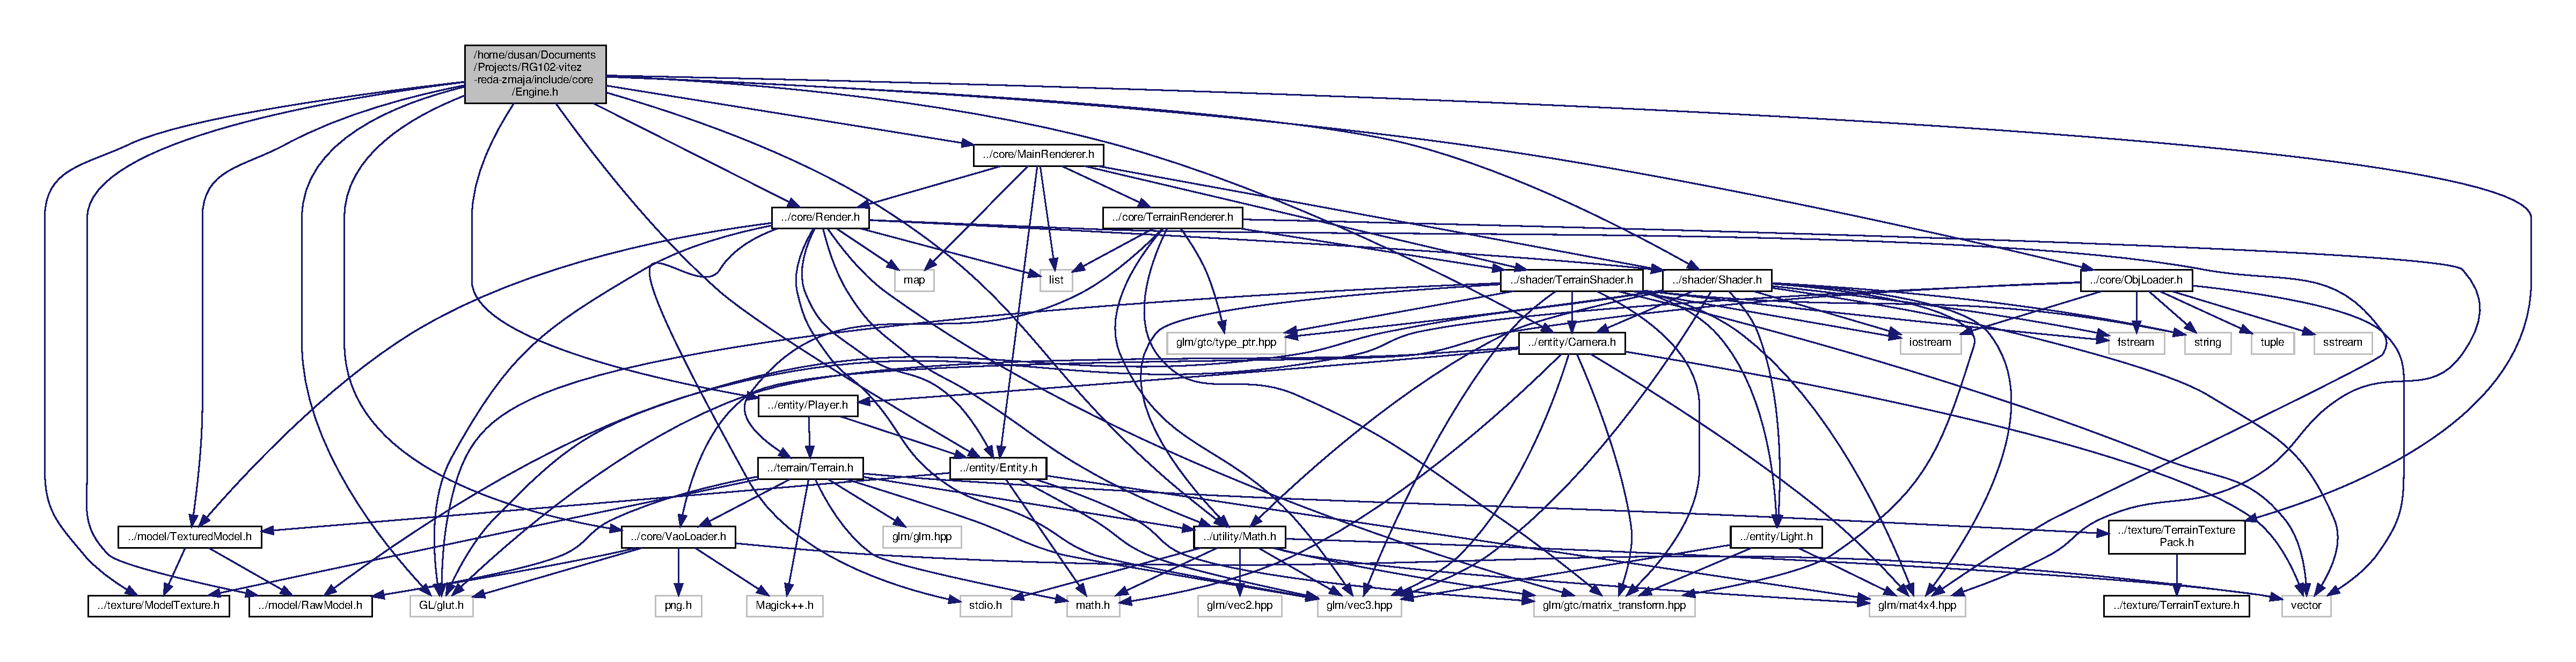
\includegraphics[width=350pt]{Engine_8h__incl}
\end{center}
\end{figure}
Ovaj graf pokazuje koje datoteke direktno ili indirektno uključuju ovu datoteku\+: \nopagebreak
\begin{figure}[H]
\begin{center}
\leavevmode
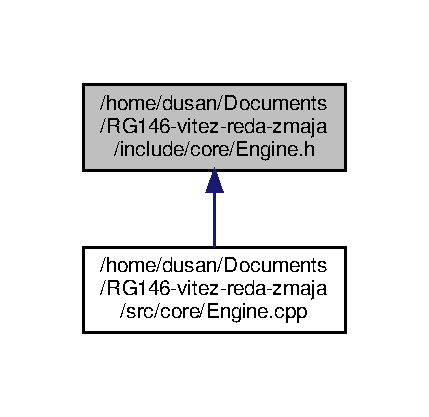
\includegraphics[width=238pt]{Engine_8h__dep__incl}
\end{center}
\end{figure}
\subsection*{Klase, strukture i unije}
\begin{DoxyCompactItemize}
\item 
class \hyperlink{classcore_1_1Engine}{core\+::\+Engine}
\begin{DoxyCompactList}\small\item\em Klasa \hyperlink{classcore_1_1Engine}{Engine} je jezgro i kontroler programa. Sva bitnija podesavanja i inicijalizacije desavaju se u ovoj klasi. Klasa je zaduzena za inicijalizaciju G\+L\+U\+T-\/a , Open\+G\+L-\/a, i kontrolisanje i kreiranje ostalih korisnicki definisanih klasa i funkcija. \end{DoxyCompactList}\end{DoxyCompactItemize}
\subsection*{Prostori imena}
\begin{DoxyCompactItemize}
\item 
 \hyperlink{namespacecore}{core}
\begin{DoxyCompactList}\small\item\em Prostor imena core. Sadrzi sve klase, funkcije i promenljive koje su od sustinskog znacaja za funkcionisanje programa. \end{DoxyCompactList}\end{DoxyCompactItemize}
\subsection*{Makro zamene}
\begin{DoxyCompactItemize}
\item 
\#define \hyperlink{Engine_8h_a4af1b6159e447ba72652bb7fcdfa726e}{E\+SC}~27
\end{DoxyCompactItemize}
\subsection*{Funkcije}
\begin{DoxyCompactItemize}
\item 
void \hyperlink{namespacecore_a1c3be366234e051e17b4b45f40c18960}{core\+::render\+Scene} (void)
\begin{DoxyCompactList}\small\item\em Callback funkcija. Pokazivac funkcije prosledjuje se funkciji glut\+Display\+Func(). Funkcija koja kontrolise sta ce biti iscrtano na ekranu. \end{DoxyCompactList}\item 
void \hyperlink{namespacecore_a179fad39a2b3f74cf7a0bffb578fce00}{core\+::on\+Keyboard} (unsigned char key, int x, int y)
\begin{DoxyCompactList}\small\item\em Callback funkcija. Pokazivac funkcije prosledjuje se funkciji glut\+Keyboard\+Func(). Funkcija koja proverava ulaz sa tastature. \end{DoxyCompactList}\item 
void \hyperlink{namespacecore_a581fd18fb14102b9234a113bc95341b4}{core\+::on\+Mouse} (int button, int state, int x, int y)
\begin{DoxyCompactList}\small\item\em Callback funkcija. Pokazivac funkcije prosledjuje se funkciji glut\+Mouse\+Func(). Funkcija koja proverava ulaz sa misa. \end{DoxyCompactList}\item 
void \hyperlink{namespacecore_a3ad12cad5f74289de4ad97762e453621}{core\+::on\+Special\+Down} (int key, int x, int y)
\begin{DoxyCompactList}\small\item\em Callback funkcija. Pokazivac funkcije prosledjuje se funkciji glut\+Special\+Func(). Funkcija koja proverava pritisnuti specijalni karakter. \end{DoxyCompactList}\item 
void \hyperlink{namespacecore_a590273d60aac2764ebf098f1b9aab3fe}{core\+::on\+Special\+Up} (int key, int x, int y)
\begin{DoxyCompactList}\small\item\em Callback funkcija. Pokazivac funkcije prosledjuje se funkciji glut\+Special\+Up\+Func(). Funkcija koja proverava otpusteni specijalni karakter. \end{DoxyCompactList}\end{DoxyCompactItemize}


\subsection{Opširniji opis}
Deklaracija klase Engine i deklaracija callback funkcija. 

\begin{DoxyAuthor}{Autor}
Dusan Pantelic 
\end{DoxyAuthor}
\begin{DoxyDate}{Datum}
Decembar 2017 
\end{DoxyDate}


\subsection{Dokumentacija makro zamene}
\mbox{\Hypertarget{Engine_8h_a4af1b6159e447ba72652bb7fcdfa726e}\label{Engine_8h_a4af1b6159e447ba72652bb7fcdfa726e}} 
\index{Engine.\+h@{Engine.\+h}!E\+SC@{E\+SC}}
\index{E\+SC@{E\+SC}!Engine.\+h@{Engine.\+h}}
\subsubsection{\texorpdfstring{E\+SC}{ESC}}
{\footnotesize\ttfamily \#define E\+SC~27}


\hypertarget{MainRenderer_8h}{}\section{Opis datoteke /home/dusan/\+Documents/\+R\+G146-\/vitez-\/reda-\/zmaja/include/core/\+Main\+Renderer.h}
\label{MainRenderer_8h}\index{/home/dusan/\+Documents/\+R\+G146-\/vitez-\/reda-\/zmaja/include/core/\+Main\+Renderer.\+h@{/home/dusan/\+Documents/\+R\+G146-\/vitez-\/reda-\/zmaja/include/core/\+Main\+Renderer.\+h}}


Deklaracija klase Render.  


{\ttfamily \#include \char`\"{}../core/\+Render.\+h\char`\"{}}\newline
{\ttfamily \#include \char`\"{}../shader/\+Shader.\+h\char`\"{}}\newline
{\ttfamily \#include \char`\"{}../core/\+Terrain\+Renderer.\+h\char`\"{}}\newline
{\ttfamily \#include \char`\"{}../shader/\+Terrain\+Shader.\+h\char`\"{}}\newline
{\ttfamily \#include \char`\"{}../entity/\+Entity.\+h\char`\"{}}\newline
{\ttfamily \#include \char`\"{}../core/\+Skybox\+Renderer.\+h\char`\"{}}\newline
{\ttfamily \#include \char`\"{}../core/\+Vao\+Loader.\+h\char`\"{}}\newline
{\ttfamily \#include $<$map$>$}\newline
{\ttfamily \#include $<$list$>$}\newline
Graf zavisnosti datoteka za Main\+Renderer.\+h\+:\nopagebreak
\begin{figure}[H]
\begin{center}
\leavevmode
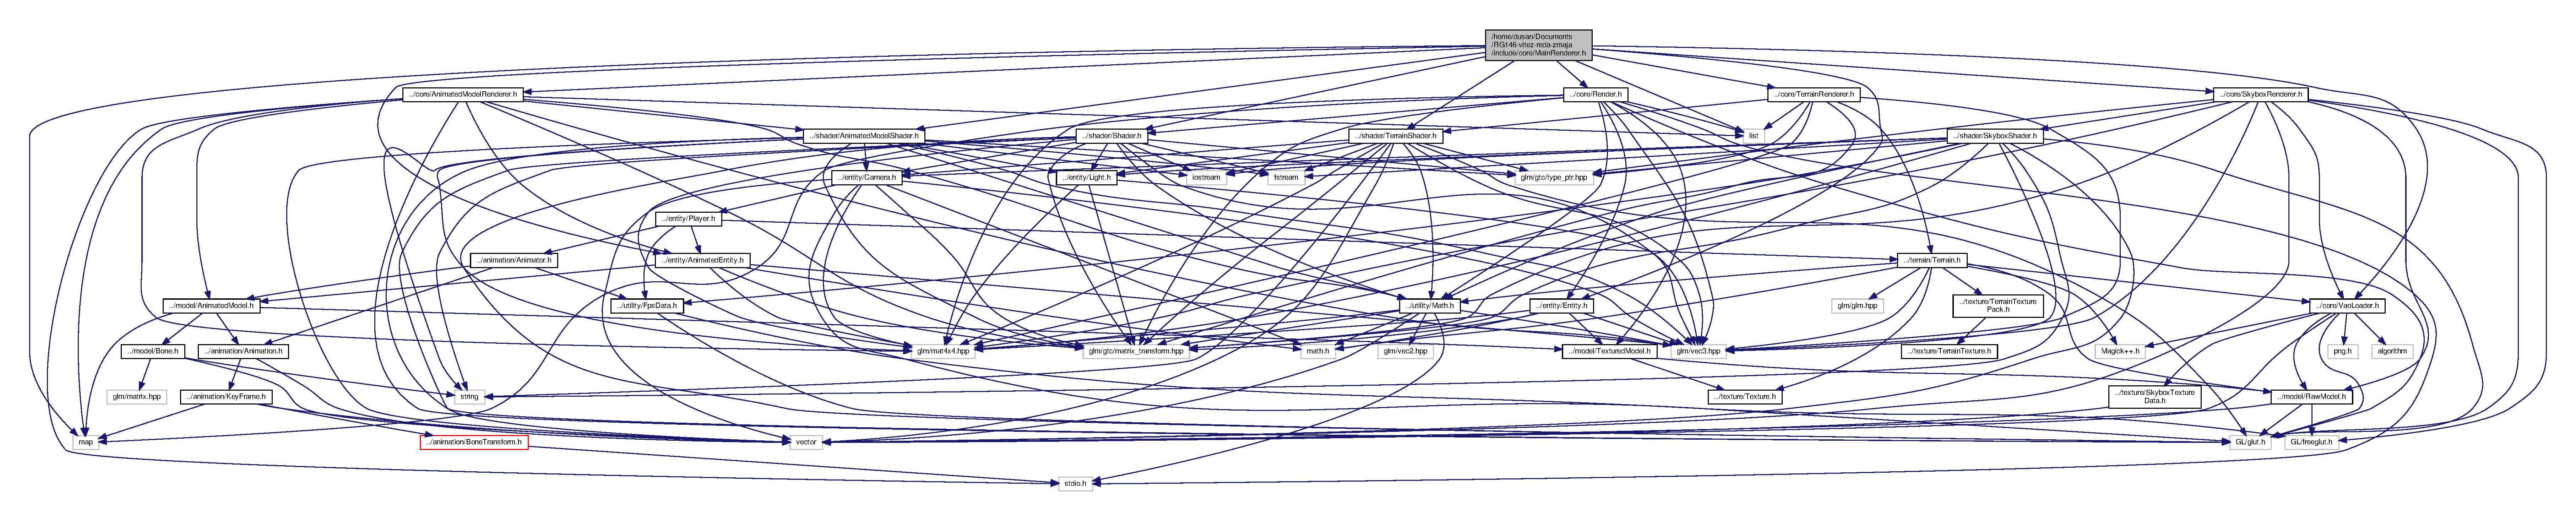
\includegraphics[width=350pt]{MainRenderer_8h__incl}
\end{center}
\end{figure}
Ovaj graf pokazuje koje datoteke direktno ili indirektno uključuju ovu datoteku\+: \nopagebreak
\begin{figure}[H]
\begin{center}
\leavevmode
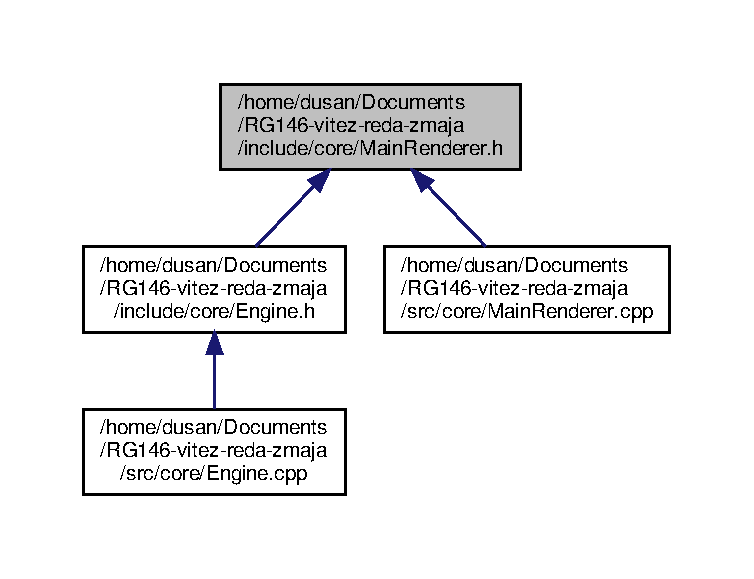
\includegraphics[width=350pt]{MainRenderer_8h__dep__incl}
\end{center}
\end{figure}
\subsection*{Klase, strukture i unije}
\begin{DoxyCompactItemize}
\item 
class \hyperlink{classcore_1_1MainRenderer}{core\+::\+Main\+Renderer}
\begin{DoxyCompactList}\small\item\em Klasa \hyperlink{classcore_1_1MainRenderer}{Main\+Renderer} je zaduzena za iscrtavanje sadrzaja na ekran. Tokom pokretanja prvo se vrsi priprema za iscrtavanje, a zatim se iscrtavaju teren igrac i ostali entiteti. \end{DoxyCompactList}\end{DoxyCompactItemize}
\subsection*{Prostori imena}
\begin{DoxyCompactItemize}
\item 
 \hyperlink{namespacecore}{core}
\begin{DoxyCompactList}\small\item\em Prostor imena core. Sadrzi sve klase, funkcije i promenljive koje su od sustinskog znacaja za funkcionisanje programa. \end{DoxyCompactList}\end{DoxyCompactItemize}
\subsection*{Makro zamene}
\begin{DoxyCompactItemize}
\item 
\#define \hyperlink{MainRenderer_8h_a180102dba1103db19570c71c6f25eb1c}{V\+E\+R\+T\+E\+X\+\_\+\+F\+I\+LE}~\char`\"{}src/shader/Vertex\+Shader.\+txt\char`\"{}
\item 
\#define \hyperlink{MainRenderer_8h_a30d830937cb33de7ec847474ed321d2d}{F\+R\+A\+G\+M\+E\+N\+T\+\_\+\+F\+I\+LE}~\char`\"{}src/shader/Fragment\+Shader.\+txt\char`\"{}
\item 
\#define \hyperlink{MainRenderer_8h_af318b4f457d085d5d0d437f7008f9416}{T\+E\+R\+R\+A\+I\+N\+\_\+\+V\+E\+R\+T\+E\+X\+\_\+\+F\+I\+LE}~\char`\"{}src/shader/Terrain\+Vertex\+Shader.\+txt\char`\"{}
\item 
\#define \hyperlink{MainRenderer_8h_ae0f5765ea8e4bfeea87a86374508e4fb}{T\+E\+R\+R\+A\+I\+N\+\_\+\+F\+R\+A\+G\+M\+E\+N\+T\+\_\+\+F\+I\+LE}~\char`\"{}src/shader/Terrain\+Fragment\+Shader.\+txt\char`\"{}
\item 
\#define \hyperlink{MainRenderer_8h_a5c71a5e59a53413cd6c270266d63b031}{R}~0.\+6
\item 
\#define \hyperlink{MainRenderer_8h_aed9ea78689ecce0b7264c02c7f8a9a54}{G}~0.\+6
\item 
\#define \hyperlink{MainRenderer_8h_a111da81ae5883147168bbb8366377b10}{B}~0.\+6
\end{DoxyCompactItemize}


\subsection{Opširniji opis}
Deklaracija klase Render. 

\begin{DoxyAuthor}{Autor}
Dusan Pantelic 
\end{DoxyAuthor}
\begin{DoxyDate}{Datum}
Avgvust 2018 
\end{DoxyDate}


\subsection{Dokumentacija makro zamene}
\mbox{\Hypertarget{MainRenderer_8h_a111da81ae5883147168bbb8366377b10}\label{MainRenderer_8h_a111da81ae5883147168bbb8366377b10}} 
\index{Main\+Renderer.\+h@{Main\+Renderer.\+h}!B@{B}}
\index{B@{B}!Main\+Renderer.\+h@{Main\+Renderer.\+h}}
\subsubsection{\texorpdfstring{B}{B}}
{\footnotesize\ttfamily \#define B~0.\+6}

\mbox{\Hypertarget{MainRenderer_8h_a30d830937cb33de7ec847474ed321d2d}\label{MainRenderer_8h_a30d830937cb33de7ec847474ed321d2d}} 
\index{Main\+Renderer.\+h@{Main\+Renderer.\+h}!F\+R\+A\+G\+M\+E\+N\+T\+\_\+\+F\+I\+LE@{F\+R\+A\+G\+M\+E\+N\+T\+\_\+\+F\+I\+LE}}
\index{F\+R\+A\+G\+M\+E\+N\+T\+\_\+\+F\+I\+LE@{F\+R\+A\+G\+M\+E\+N\+T\+\_\+\+F\+I\+LE}!Main\+Renderer.\+h@{Main\+Renderer.\+h}}
\subsubsection{\texorpdfstring{F\+R\+A\+G\+M\+E\+N\+T\+\_\+\+F\+I\+LE}{FRAGMENT\_FILE}}
{\footnotesize\ttfamily \#define F\+R\+A\+G\+M\+E\+N\+T\+\_\+\+F\+I\+LE~\char`\"{}src/shader/Fragment\+Shader.\+txt\char`\"{}}

\mbox{\Hypertarget{MainRenderer_8h_aed9ea78689ecce0b7264c02c7f8a9a54}\label{MainRenderer_8h_aed9ea78689ecce0b7264c02c7f8a9a54}} 
\index{Main\+Renderer.\+h@{Main\+Renderer.\+h}!G@{G}}
\index{G@{G}!Main\+Renderer.\+h@{Main\+Renderer.\+h}}
\subsubsection{\texorpdfstring{G}{G}}
{\footnotesize\ttfamily \#define G~0.\+6}

\mbox{\Hypertarget{MainRenderer_8h_a5c71a5e59a53413cd6c270266d63b031}\label{MainRenderer_8h_a5c71a5e59a53413cd6c270266d63b031}} 
\index{Main\+Renderer.\+h@{Main\+Renderer.\+h}!R@{R}}
\index{R@{R}!Main\+Renderer.\+h@{Main\+Renderer.\+h}}
\subsubsection{\texorpdfstring{R}{R}}
{\footnotesize\ttfamily \#define R~0.\+6}

\mbox{\Hypertarget{MainRenderer_8h_ae0f5765ea8e4bfeea87a86374508e4fb}\label{MainRenderer_8h_ae0f5765ea8e4bfeea87a86374508e4fb}} 
\index{Main\+Renderer.\+h@{Main\+Renderer.\+h}!T\+E\+R\+R\+A\+I\+N\+\_\+\+F\+R\+A\+G\+M\+E\+N\+T\+\_\+\+F\+I\+LE@{T\+E\+R\+R\+A\+I\+N\+\_\+\+F\+R\+A\+G\+M\+E\+N\+T\+\_\+\+F\+I\+LE}}
\index{T\+E\+R\+R\+A\+I\+N\+\_\+\+F\+R\+A\+G\+M\+E\+N\+T\+\_\+\+F\+I\+LE@{T\+E\+R\+R\+A\+I\+N\+\_\+\+F\+R\+A\+G\+M\+E\+N\+T\+\_\+\+F\+I\+LE}!Main\+Renderer.\+h@{Main\+Renderer.\+h}}
\subsubsection{\texorpdfstring{T\+E\+R\+R\+A\+I\+N\+\_\+\+F\+R\+A\+G\+M\+E\+N\+T\+\_\+\+F\+I\+LE}{TERRAIN\_FRAGMENT\_FILE}}
{\footnotesize\ttfamily \#define T\+E\+R\+R\+A\+I\+N\+\_\+\+F\+R\+A\+G\+M\+E\+N\+T\+\_\+\+F\+I\+LE~\char`\"{}src/shader/Terrain\+Fragment\+Shader.\+txt\char`\"{}}

\mbox{\Hypertarget{MainRenderer_8h_af318b4f457d085d5d0d437f7008f9416}\label{MainRenderer_8h_af318b4f457d085d5d0d437f7008f9416}} 
\index{Main\+Renderer.\+h@{Main\+Renderer.\+h}!T\+E\+R\+R\+A\+I\+N\+\_\+\+V\+E\+R\+T\+E\+X\+\_\+\+F\+I\+LE@{T\+E\+R\+R\+A\+I\+N\+\_\+\+V\+E\+R\+T\+E\+X\+\_\+\+F\+I\+LE}}
\index{T\+E\+R\+R\+A\+I\+N\+\_\+\+V\+E\+R\+T\+E\+X\+\_\+\+F\+I\+LE@{T\+E\+R\+R\+A\+I\+N\+\_\+\+V\+E\+R\+T\+E\+X\+\_\+\+F\+I\+LE}!Main\+Renderer.\+h@{Main\+Renderer.\+h}}
\subsubsection{\texorpdfstring{T\+E\+R\+R\+A\+I\+N\+\_\+\+V\+E\+R\+T\+E\+X\+\_\+\+F\+I\+LE}{TERRAIN\_VERTEX\_FILE}}
{\footnotesize\ttfamily \#define T\+E\+R\+R\+A\+I\+N\+\_\+\+V\+E\+R\+T\+E\+X\+\_\+\+F\+I\+LE~\char`\"{}src/shader/Terrain\+Vertex\+Shader.\+txt\char`\"{}}

\mbox{\Hypertarget{MainRenderer_8h_a180102dba1103db19570c71c6f25eb1c}\label{MainRenderer_8h_a180102dba1103db19570c71c6f25eb1c}} 
\index{Main\+Renderer.\+h@{Main\+Renderer.\+h}!V\+E\+R\+T\+E\+X\+\_\+\+F\+I\+LE@{V\+E\+R\+T\+E\+X\+\_\+\+F\+I\+LE}}
\index{V\+E\+R\+T\+E\+X\+\_\+\+F\+I\+LE@{V\+E\+R\+T\+E\+X\+\_\+\+F\+I\+LE}!Main\+Renderer.\+h@{Main\+Renderer.\+h}}
\subsubsection{\texorpdfstring{V\+E\+R\+T\+E\+X\+\_\+\+F\+I\+LE}{VERTEX\_FILE}}
{\footnotesize\ttfamily \#define V\+E\+R\+T\+E\+X\+\_\+\+F\+I\+LE~\char`\"{}src/shader/Vertex\+Shader.\+txt\char`\"{}}


\hypertarget{ObjLoader_8h}{}\section{Opis datoteke /home/dusan/\+Documents/\+R\+G146-\/vitez-\/reda-\/zmaja/include/core/\+Obj\+Loader.h}
\label{ObjLoader_8h}\index{/home/dusan/\+Documents/\+R\+G146-\/vitez-\/reda-\/zmaja/include/core/\+Obj\+Loader.\+h@{/home/dusan/\+Documents/\+R\+G146-\/vitez-\/reda-\/zmaja/include/core/\+Obj\+Loader.\+h}}


Deklaracija klase Render.  


{\ttfamily \#include \char`\"{}../core/\+Vao\+Loader.\+h\char`\"{}}\newline
{\ttfamily \#include \char`\"{}../model/\+Raw\+Model.\+h\char`\"{}}\newline
{\ttfamily \#include $<$vector$>$}\newline
{\ttfamily \#include $<$string$>$}\newline
{\ttfamily \#include $<$sstream$>$}\newline
{\ttfamily \#include $<$fstream$>$}\newline
{\ttfamily \#include $<$iostream$>$}\newline
{\ttfamily \#include $<$tuple$>$}\newline
Graf zavisnosti datoteka za Obj\+Loader.\+h\+:\nopagebreak
\begin{figure}[H]
\begin{center}
\leavevmode
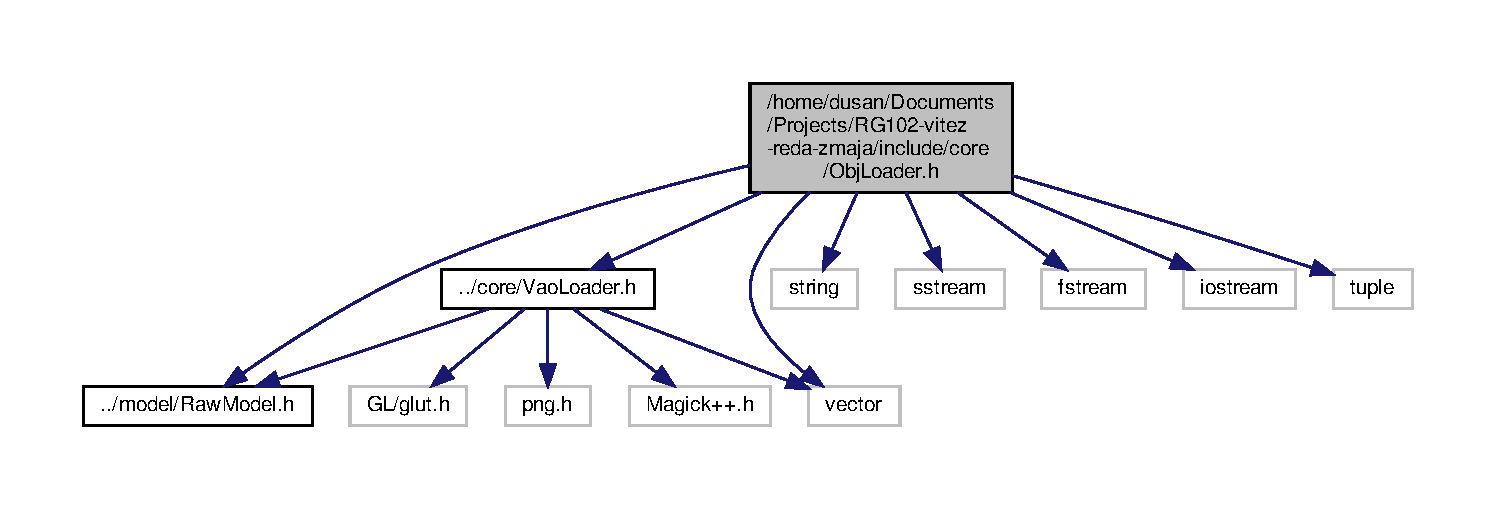
\includegraphics[width=350pt]{ObjLoader_8h__incl}
\end{center}
\end{figure}
Ovaj graf pokazuje koje datoteke direktno ili indirektno uključuju ovu datoteku\+: \nopagebreak
\begin{figure}[H]
\begin{center}
\leavevmode
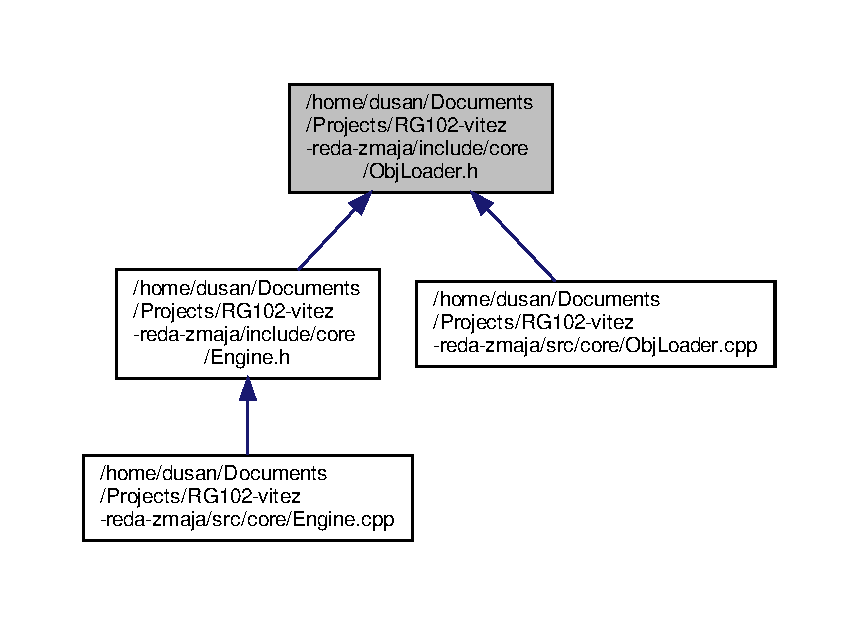
\includegraphics[width=350pt]{ObjLoader_8h__dep__incl}
\end{center}
\end{figure}
\subsection*{Klase, strukture i unije}
\begin{DoxyCompactItemize}
\item 
class \hyperlink{classcore_1_1ObjLoader}{core\+::\+Obj\+Loader}
\begin{DoxyCompactList}\small\item\em Klasa \hyperlink{classcore_1_1ObjLoader}{Obj\+Loader} je zaduzena za ucitavanje obj fajlova. Tokom pokretanja citaju se obj fajlovi koji se zatim obradjuju i podaci se prosledjuju drugim klasama koje ih koriste. \end{DoxyCompactList}\end{DoxyCompactItemize}
\subsection*{Prostori imena}
\begin{DoxyCompactItemize}
\item 
 \hyperlink{namespacecore}{core}
\begin{DoxyCompactList}\small\item\em Prostor imena core. Sadrzi sve klase, funkcije i promenljive koje su od sustinskog znacaja za funkcionisanje programa. \end{DoxyCompactList}\end{DoxyCompactItemize}


\subsection{Opširniji opis}
Deklaracija klase Render. 

\begin{DoxyAuthor}{Autor}
Dusan Pantelic 
\end{DoxyAuthor}
\begin{DoxyDate}{Datum}
Maj 2018 
\end{DoxyDate}

\hypertarget{Render_8h}{}\section{Opis datoteke /home/dusan/\+Documents/\+R\+G146-\/vitez-\/reda-\/zmaja/include/core/\+Render.h}
\label{Render_8h}\index{/home/dusan/\+Documents/\+R\+G146-\/vitez-\/reda-\/zmaja/include/core/\+Render.\+h@{/home/dusan/\+Documents/\+R\+G146-\/vitez-\/reda-\/zmaja/include/core/\+Render.\+h}}


Deklaracija klase Render.  


{\ttfamily \#include \char`\"{}../model/\+Textured\+Model.\+h\char`\"{}}\newline
{\ttfamily \#include \char`\"{}../entity/\+Entity.\+h\char`\"{}}\newline
{\ttfamily \#include \char`\"{}../utility/\+Math.\+h\char`\"{}}\newline
{\ttfamily \#include \char`\"{}../shader/\+Shader.\+h\char`\"{}}\newline
{\ttfamily \#include $<$G\+L/glut.\+h$>$}\newline
{\ttfamily \#include $<$stdio.\+h$>$}\newline
{\ttfamily \#include $<$map$>$}\newline
{\ttfamily \#include $<$list$>$}\newline
{\ttfamily \#include $<$glm/vec3.\+hpp$>$}\newline
{\ttfamily \#include $<$glm/mat4x4.\+hpp$>$}\newline
{\ttfamily \#include $<$glm/gtc/matrix\+\_\+transform.\+hpp$>$}\newline
Graf zavisnosti datoteka za Render.\+h\+:\nopagebreak
\begin{figure}[H]
\begin{center}
\leavevmode
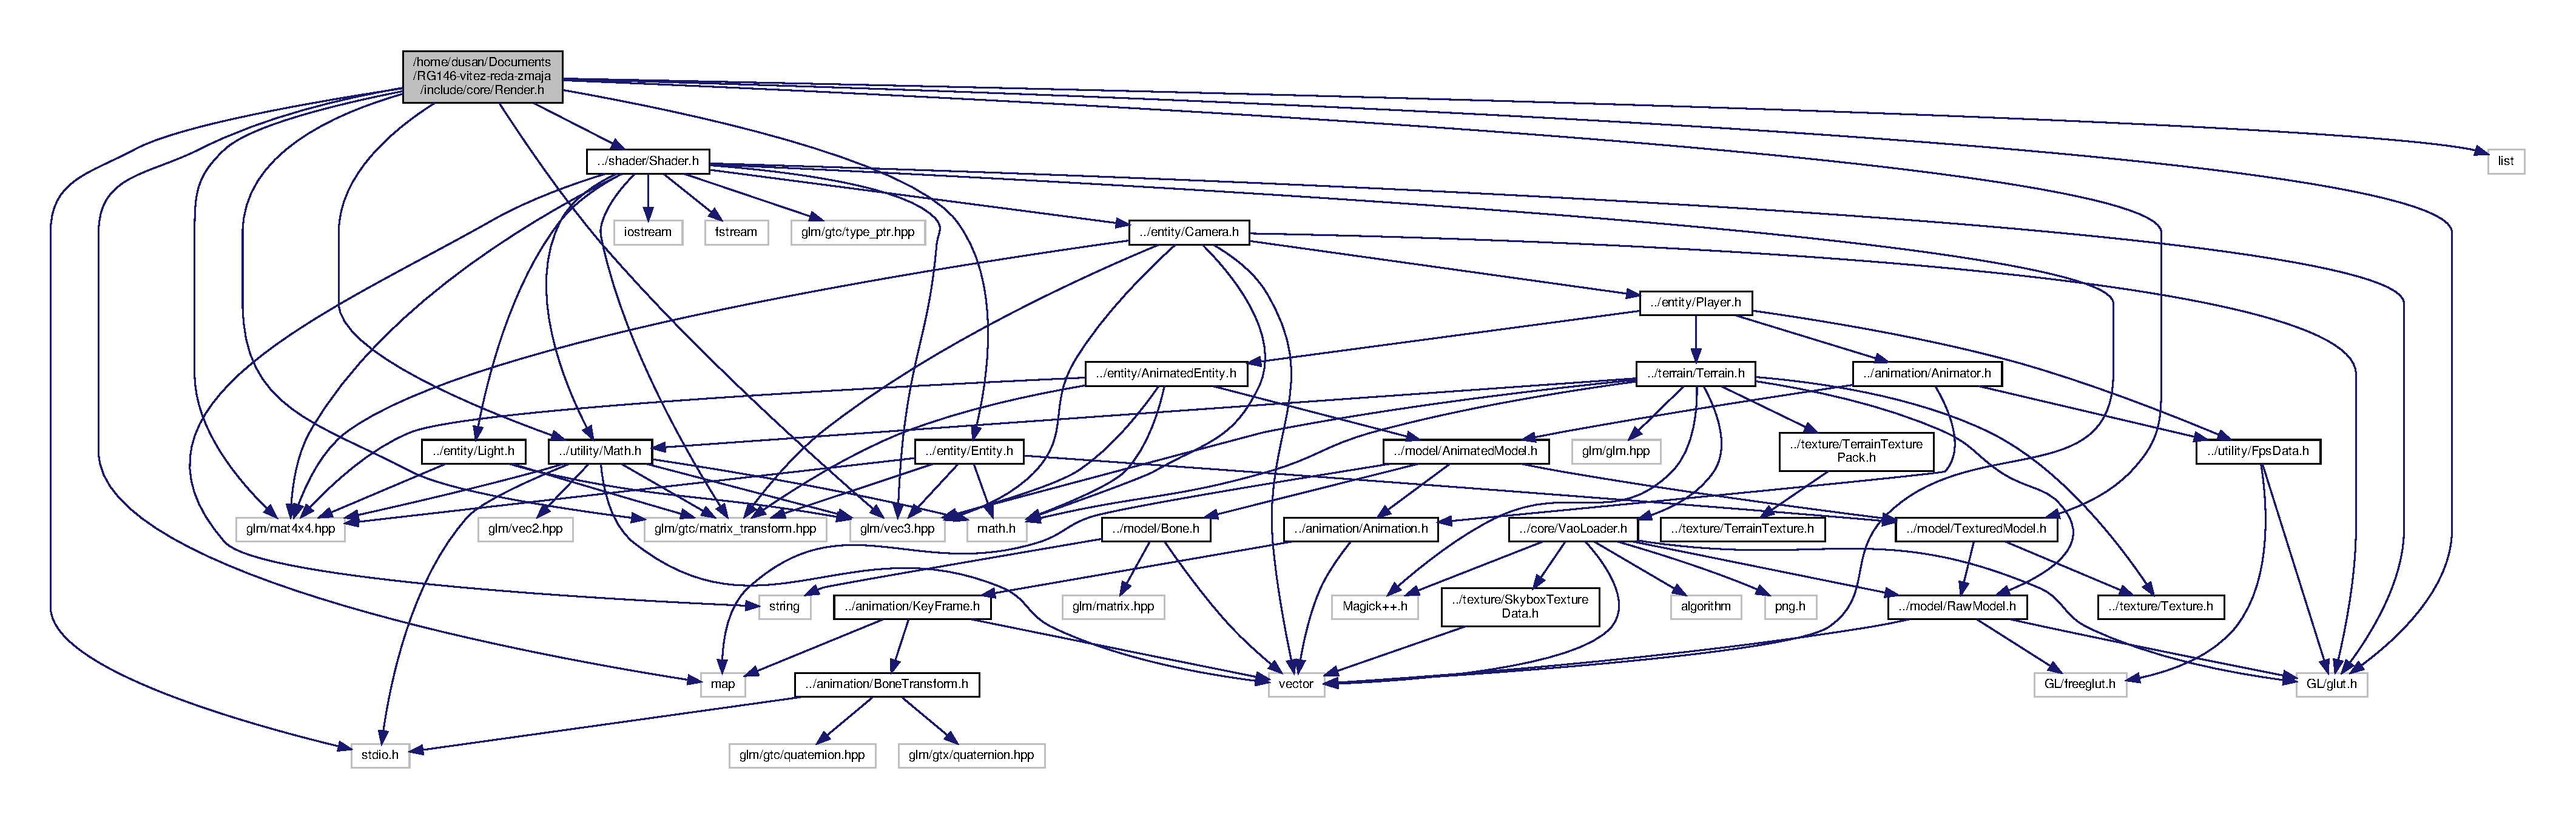
\includegraphics[width=350pt]{Render_8h__incl}
\end{center}
\end{figure}
Ovaj graf pokazuje koje datoteke direktno ili indirektno uključuju ovu datoteku\+: \nopagebreak
\begin{figure}[H]
\begin{center}
\leavevmode
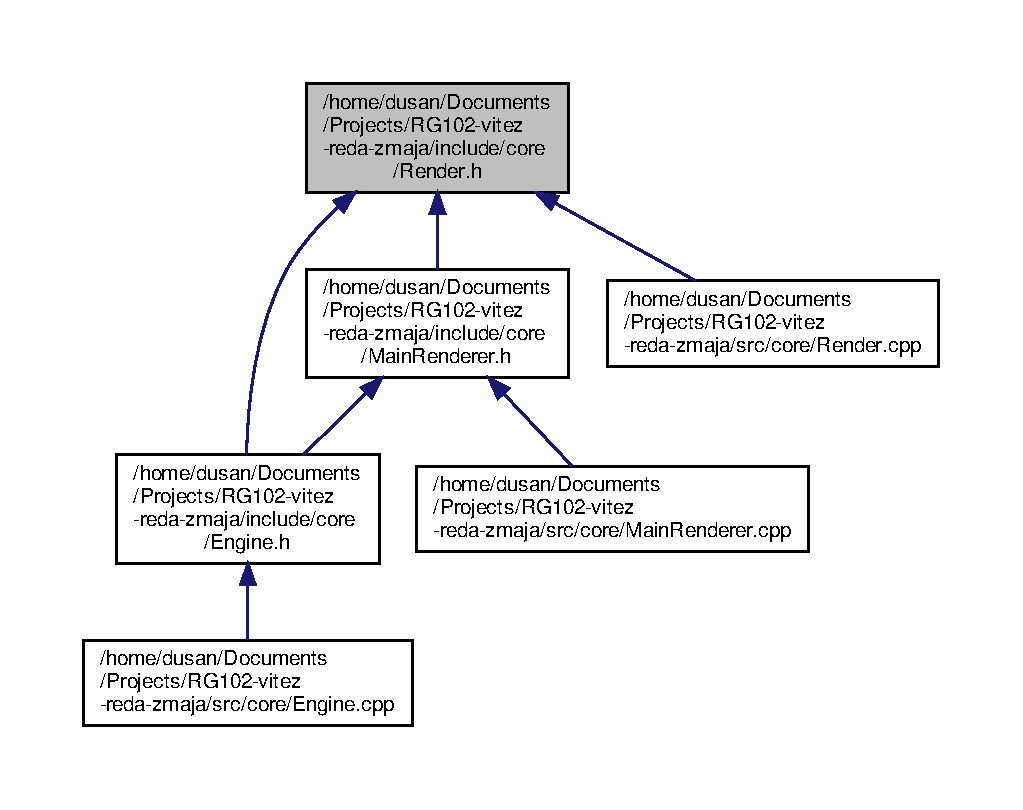
\includegraphics[width=350pt]{Render_8h__dep__incl}
\end{center}
\end{figure}
\subsection*{Klase, strukture i unije}
\begin{DoxyCompactItemize}
\item 
class \hyperlink{classcore_1_1Render}{core\+::\+Render}
\begin{DoxyCompactList}\small\item\em Klasa \hyperlink{classcore_1_1Render}{Render} je zaduzena za iscrtavanje entiteta na ekran. Tokom pokretanja prvo se vrsi priprema za iscrtavanje, a zatim se sadrzaj niza atributa(koordinate, boje, texture ...) iscrtava na ekran. \end{DoxyCompactList}\end{DoxyCompactItemize}
\subsection*{Prostori imena}
\begin{DoxyCompactItemize}
\item 
 \hyperlink{namespacecore}{core}
\begin{DoxyCompactList}\small\item\em Prostor imena core. Sadrzi sve klase, funkcije i promenljive koje su od sustinskog znacaja za funkcionisanje programa. \end{DoxyCompactList}\end{DoxyCompactItemize}
\subsection*{Makro zamene}
\begin{DoxyCompactItemize}
\item 
\#define \hyperlink{Render_8h_a120fb070bddb21f0bd899f50252c4cb5}{G\+L\+\_\+\+G\+L\+E\+X\+T\+\_\+\+P\+R\+O\+T\+O\+T\+Y\+P\+ES}
\end{DoxyCompactItemize}


\subsection{Opširniji opis}
Deklaracija klase Render. 

\begin{DoxyAuthor}{Autor}
Dusan Pantelic 
\end{DoxyAuthor}
\begin{DoxyDate}{Datum}
Decembar 2017 
\end{DoxyDate}


\subsection{Dokumentacija makro zamene}
\mbox{\Hypertarget{Render_8h_a120fb070bddb21f0bd899f50252c4cb5}\label{Render_8h_a120fb070bddb21f0bd899f50252c4cb5}} 
\index{Render.\+h@{Render.\+h}!G\+L\+\_\+\+G\+L\+E\+X\+T\+\_\+\+P\+R\+O\+T\+O\+T\+Y\+P\+ES@{G\+L\+\_\+\+G\+L\+E\+X\+T\+\_\+\+P\+R\+O\+T\+O\+T\+Y\+P\+ES}}
\index{G\+L\+\_\+\+G\+L\+E\+X\+T\+\_\+\+P\+R\+O\+T\+O\+T\+Y\+P\+ES@{G\+L\+\_\+\+G\+L\+E\+X\+T\+\_\+\+P\+R\+O\+T\+O\+T\+Y\+P\+ES}!Render.\+h@{Render.\+h}}
\subsubsection{\texorpdfstring{G\+L\+\_\+\+G\+L\+E\+X\+T\+\_\+\+P\+R\+O\+T\+O\+T\+Y\+P\+ES}{GL\_GLEXT\_PROTOTYPES}}
{\footnotesize\ttfamily \#define G\+L\+\_\+\+G\+L\+E\+X\+T\+\_\+\+P\+R\+O\+T\+O\+T\+Y\+P\+ES}


\hypertarget{TerrainRenderer_8h}{}\section{Opis datoteke /home/dusan/\+Documents/\+R\+G146-\/vitez-\/reda-\/zmaja/include/core/\+Terrain\+Renderer.h}
\label{TerrainRenderer_8h}\index{/home/dusan/\+Documents/\+R\+G146-\/vitez-\/reda-\/zmaja/include/core/\+Terrain\+Renderer.\+h@{/home/dusan/\+Documents/\+R\+G146-\/vitez-\/reda-\/zmaja/include/core/\+Terrain\+Renderer.\+h}}


Deklaracija klase Terrain\+Renderer.  


{\ttfamily \#include \char`\"{}../shader/\+Terrain\+Shader.\+h\char`\"{}}\newline
{\ttfamily \#include \char`\"{}../terrain/\+Terrain.\+h\char`\"{}}\newline
{\ttfamily \#include $<$glm/vec3.\+hpp$>$}\newline
{\ttfamily \#include $<$glm/mat4x4.\+hpp$>$}\newline
{\ttfamily \#include $<$glm/gtc/matrix\+\_\+transform.\+hpp$>$}\newline
{\ttfamily \#include $<$glm/gtc/type\+\_\+ptr.\+hpp$>$}\newline
{\ttfamily \#include $<$list$>$}\newline
Graf zavisnosti datoteka za Terrain\+Renderer.\+h\+:\nopagebreak
\begin{figure}[H]
\begin{center}
\leavevmode
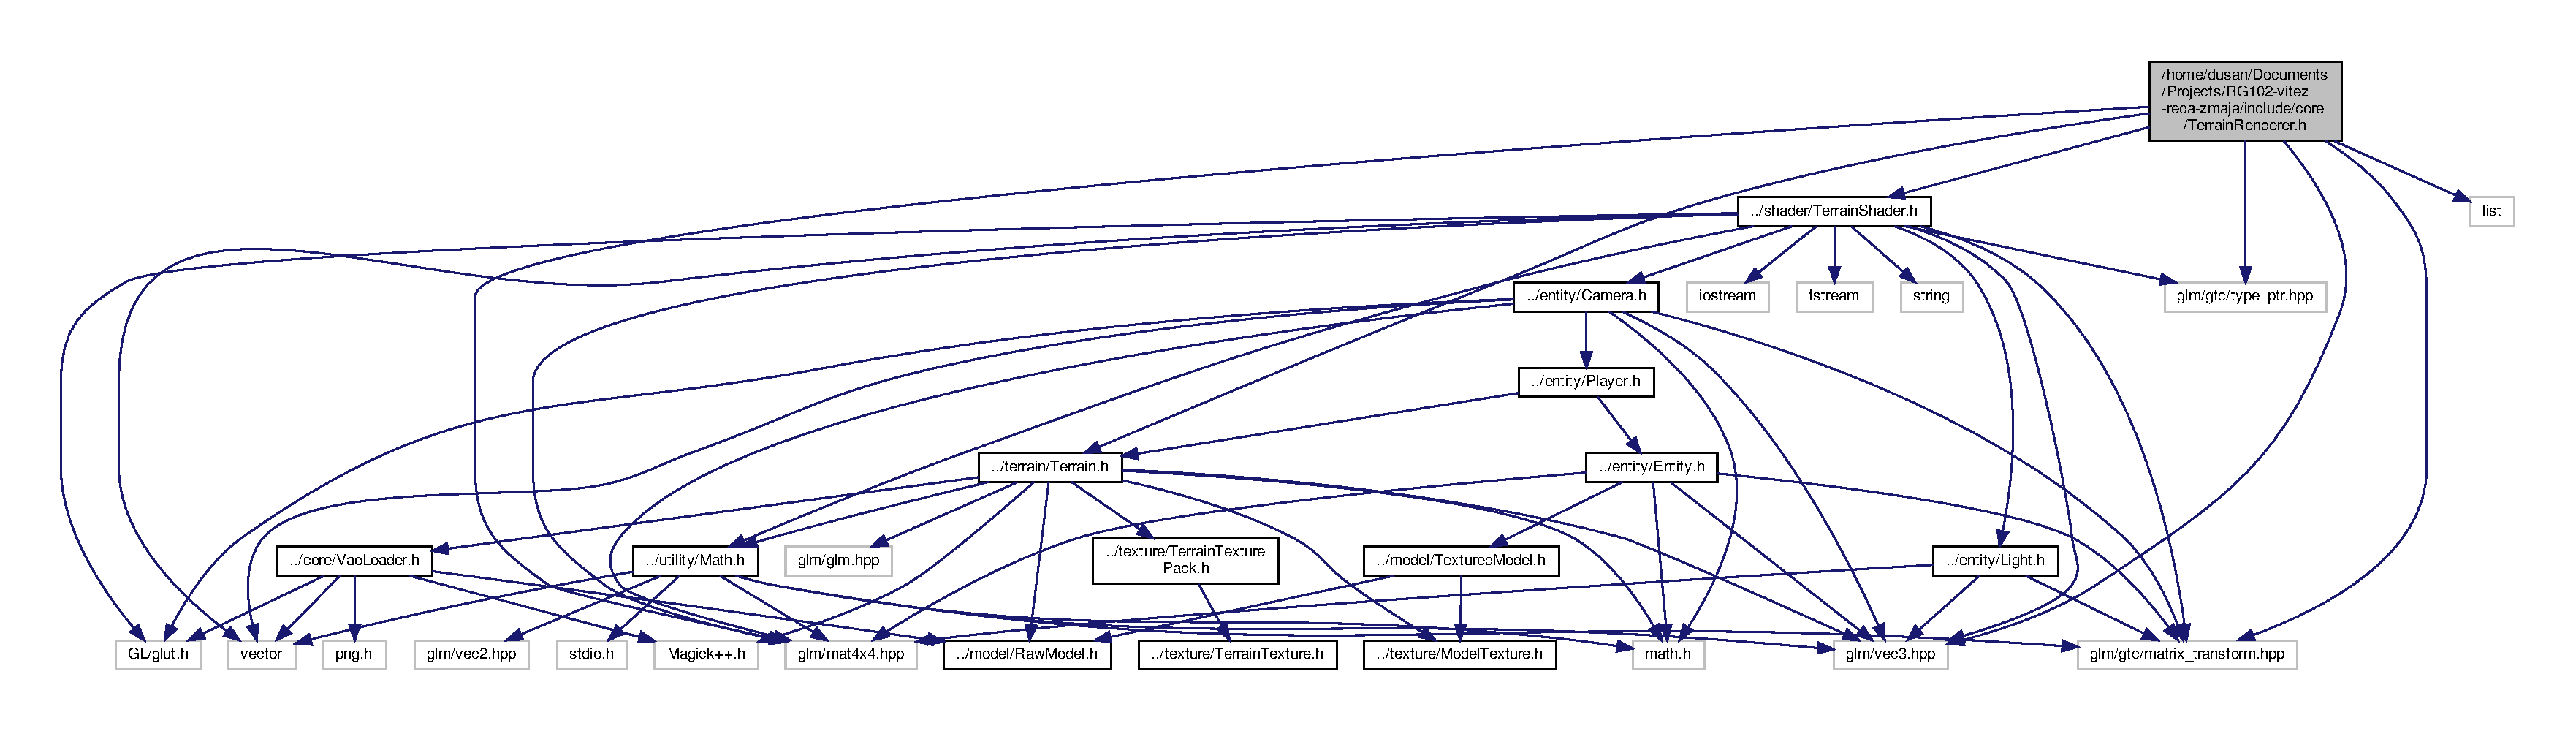
\includegraphics[width=350pt]{TerrainRenderer_8h__incl}
\end{center}
\end{figure}
Ovaj graf pokazuje koje datoteke direktno ili indirektno uključuju ovu datoteku\+: \nopagebreak
\begin{figure}[H]
\begin{center}
\leavevmode
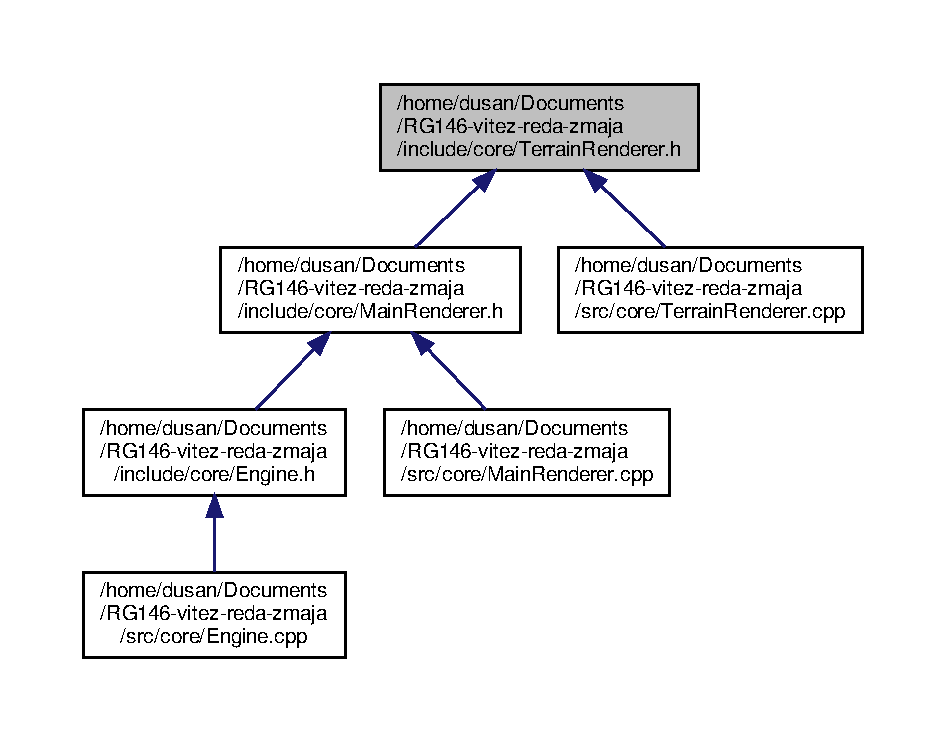
\includegraphics[width=350pt]{TerrainRenderer_8h__dep__incl}
\end{center}
\end{figure}
\subsection*{Klase, strukture i unije}
\begin{DoxyCompactItemize}
\item 
class \hyperlink{classcore_1_1TerrainRenderer}{core\+::\+Terrain\+Renderer}
\begin{DoxyCompactList}\small\item\em Klasa \hyperlink{classcore_1_1TerrainRenderer}{Terrain\+Renderer} je zaduzena za iscrtavanje terena na ekran. Tokom pokretanja prvo se vrsi priprema za iscrtavanje, a zatim se sadrzaj niza atributa(koordinate, boje, texture ...) iscrtava na ekran. \end{DoxyCompactList}\end{DoxyCompactItemize}
\subsection*{Prostori imena}
\begin{DoxyCompactItemize}
\item 
 \hyperlink{namespacecore}{core}
\begin{DoxyCompactList}\small\item\em Prostor imena core. Sadrzi sve klase, funkcije i promenljive koje su od sustinskog znacaja za funkcionisanje programa. \end{DoxyCompactList}\end{DoxyCompactItemize}


\subsection{Opširniji opis}
Deklaracija klase Terrain\+Renderer. 

\begin{DoxyAuthor}{Autor}
Dusan Pantelic 
\end{DoxyAuthor}
\begin{DoxyDate}{Datum}
Decembar 2018 
\end{DoxyDate}

\hypertarget{VaoLoader_8h}{}\section{Opis datoteke /home/dusan/\+Documents/\+Projects/\+R\+G102-\/vitez-\/reda-\/zmaja/include/core/\+Vao\+Loader.h}
\label{VaoLoader_8h}\index{/home/dusan/\+Documents/\+Projects/\+R\+G102-\/vitez-\/reda-\/zmaja/include/core/\+Vao\+Loader.\+h@{/home/dusan/\+Documents/\+Projects/\+R\+G102-\/vitez-\/reda-\/zmaja/include/core/\+Vao\+Loader.\+h}}


Deklaracija klase Vao\+Loader.  


{\ttfamily \#include \char`\"{}../model/\+Raw\+Model.\+h\char`\"{}}\newline
{\ttfamily \#include $<$G\+L/glut.\+h$>$}\newline
{\ttfamily \#include $<$png.\+h$>$}\newline
{\ttfamily \#include $<$vector$>$}\newline
{\ttfamily \#include $<$Magick++.\+h$>$}\newline
Graf zavisnosti datoteka za Vao\+Loader.\+h\+:
\nopagebreak
\begin{figure}[H]
\begin{center}
\leavevmode
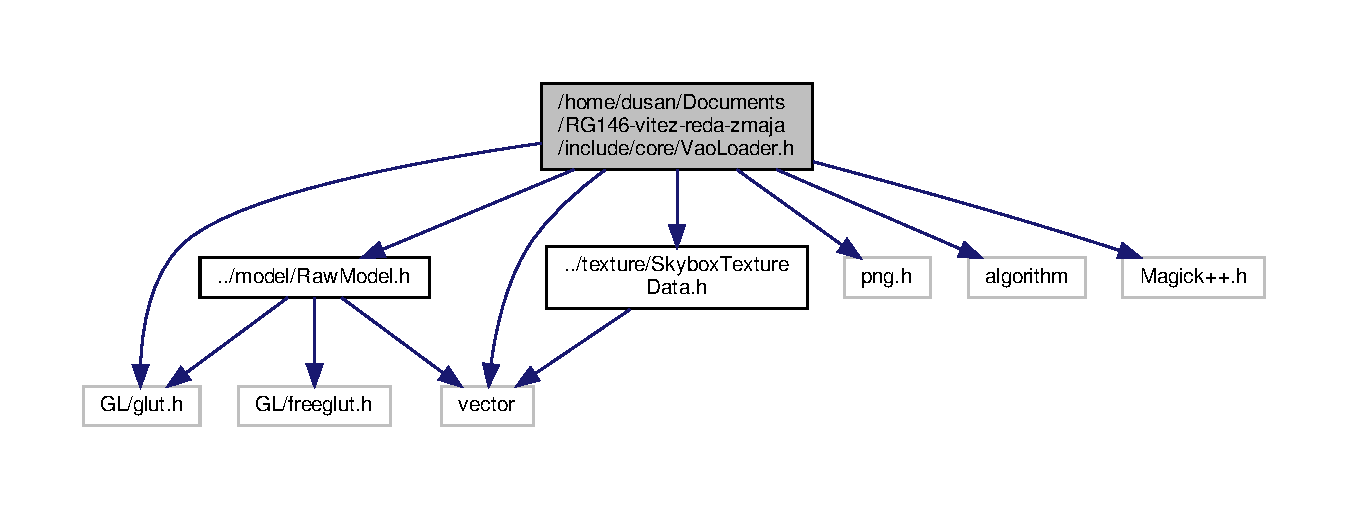
\includegraphics[width=350pt]{VaoLoader_8h__incl}
\end{center}
\end{figure}
Ovaj graf pokazuje koje datoteke direktno ili indirektno uključuju ovu datoteku\+: 
\nopagebreak
\begin{figure}[H]
\begin{center}
\leavevmode
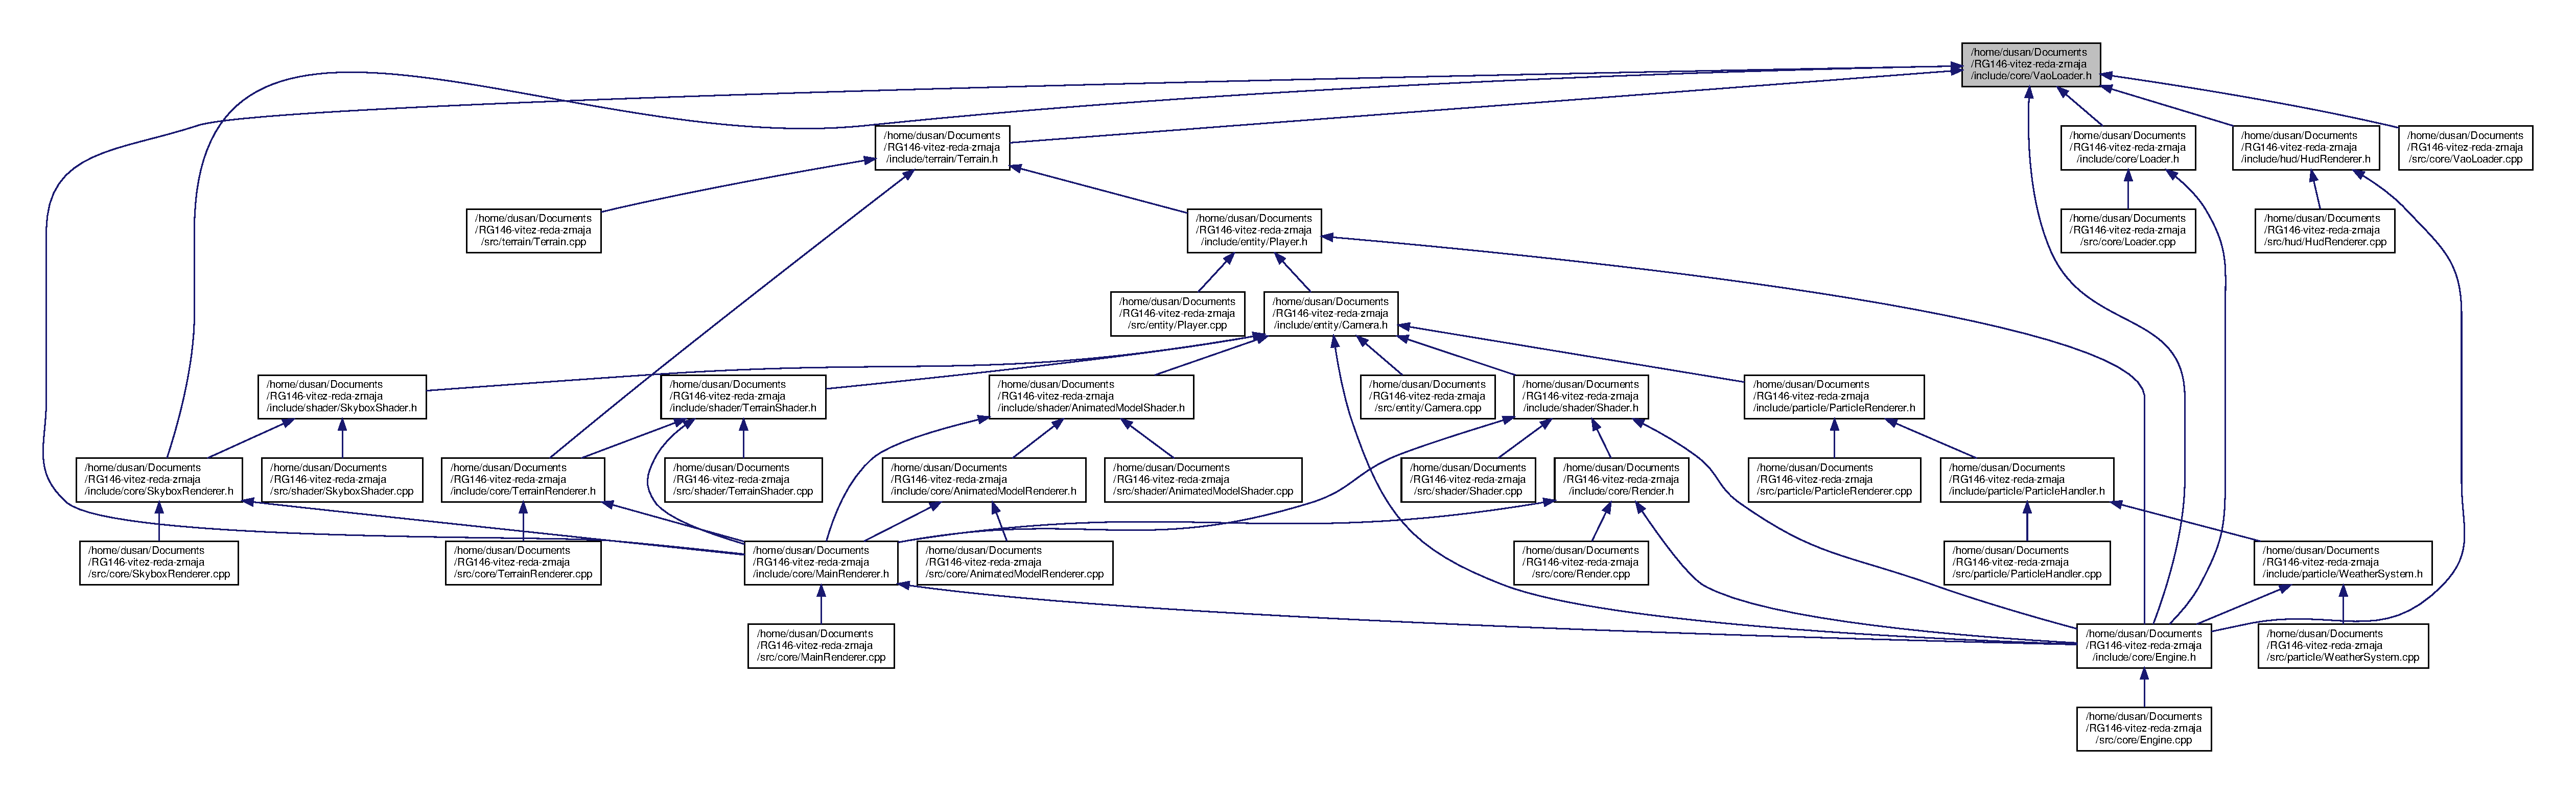
\includegraphics[width=350pt]{VaoLoader_8h__dep__incl}
\end{center}
\end{figure}
\subsection*{Klase, strukture i unije}
\begin{DoxyCompactItemize}
\item 
class \hyperlink{classcore_1_1VaoLoader}{core\+::\+Vao\+Loader}
\begin{DoxyCompactList}\small\item\em Klasa \hyperlink{classcore_1_1VaoLoader}{Vao\+Loader} je zaduzena za ucitavanje atributa u memoriju. Zadatak ove klase je ucitavanje i definisanje objekta pomocu niza atributa gde se svaki atribut ucitava u baffer koji je niz promenljivih. Ovo dovodi do komplikovanijeg koda ali kod je genericki i pomocu njega mozemo ucitavati veoma slozene objekte i texture sto bi bilo vrlo tesko kada bi smo svaki objekat sami crtali osnovnim Open\+GL funkcijama. \end{DoxyCompactList}\end{DoxyCompactItemize}
\subsection*{Prostori imena}
\begin{DoxyCompactItemize}
\item 
 \hyperlink{namespacecore}{core}
\begin{DoxyCompactList}\small\item\em Prostor imena core. Sadrzi sve klase, funkcije i promenljive koje su od sustinskog znacaja za funkcionisanje programa. \end{DoxyCompactList}\end{DoxyCompactItemize}
\subsection*{Makro zamene}
\begin{DoxyCompactItemize}
\item 
\#define \hyperlink{VaoLoader_8h_a120fb070bddb21f0bd899f50252c4cb5}{G\+L\+\_\+\+G\+L\+E\+X\+T\+\_\+\+P\+R\+O\+T\+O\+T\+Y\+P\+ES}
\end{DoxyCompactItemize}


\subsection{Opširniji opis}
Deklaracija klase Vao\+Loader. 

\begin{DoxyAuthor}{Autor}
Dusan Pantelic 
\end{DoxyAuthor}
\begin{DoxyDate}{Datum}
Decembar 2017 
\end{DoxyDate}


\subsection{Dokumentacija makro zamene}
\mbox{\Hypertarget{VaoLoader_8h_a120fb070bddb21f0bd899f50252c4cb5}\label{VaoLoader_8h_a120fb070bddb21f0bd899f50252c4cb5}} 
\index{Vao\+Loader.\+h@{Vao\+Loader.\+h}!G\+L\+\_\+\+G\+L\+E\+X\+T\+\_\+\+P\+R\+O\+T\+O\+T\+Y\+P\+ES@{G\+L\+\_\+\+G\+L\+E\+X\+T\+\_\+\+P\+R\+O\+T\+O\+T\+Y\+P\+ES}}
\index{G\+L\+\_\+\+G\+L\+E\+X\+T\+\_\+\+P\+R\+O\+T\+O\+T\+Y\+P\+ES@{G\+L\+\_\+\+G\+L\+E\+X\+T\+\_\+\+P\+R\+O\+T\+O\+T\+Y\+P\+ES}!Vao\+Loader.\+h@{Vao\+Loader.\+h}}
\subsubsection{\texorpdfstring{G\+L\+\_\+\+G\+L\+E\+X\+T\+\_\+\+P\+R\+O\+T\+O\+T\+Y\+P\+ES}{GL\_GLEXT\_PROTOTYPES}}
{\footnotesize\ttfamily \#define G\+L\+\_\+\+G\+L\+E\+X\+T\+\_\+\+P\+R\+O\+T\+O\+T\+Y\+P\+ES}


\hypertarget{Camera_8h}{}\section{Opis datoteke /home/dusan/\+Documents/\+R\+G146-\/vitez-\/reda-\/zmaja/include/entity/\+Camera.h}
\label{Camera_8h}\index{/home/dusan/\+Documents/\+R\+G146-\/vitez-\/reda-\/zmaja/include/entity/\+Camera.\+h@{/home/dusan/\+Documents/\+R\+G146-\/vitez-\/reda-\/zmaja/include/entity/\+Camera.\+h}}


Deklaracija klase Camera.  


{\ttfamily \#include \char`\"{}../entity/\+Player.\+h\char`\"{}}\newline
{\ttfamily \#include $<$vector$>$}\newline
{\ttfamily \#include $<$math.\+h$>$}\newline
{\ttfamily \#include $<$glm/vec3.\+hpp$>$}\newline
{\ttfamily \#include $<$glm/mat4x4.\+hpp$>$}\newline
{\ttfamily \#include $<$glm/gtc/matrix\+\_\+transform.\+hpp$>$}\newline
{\ttfamily \#include $<$G\+L/glut.\+h$>$}\newline
Graf zavisnosti datoteka za Camera.\+h\+:\nopagebreak
\begin{figure}[H]
\begin{center}
\leavevmode
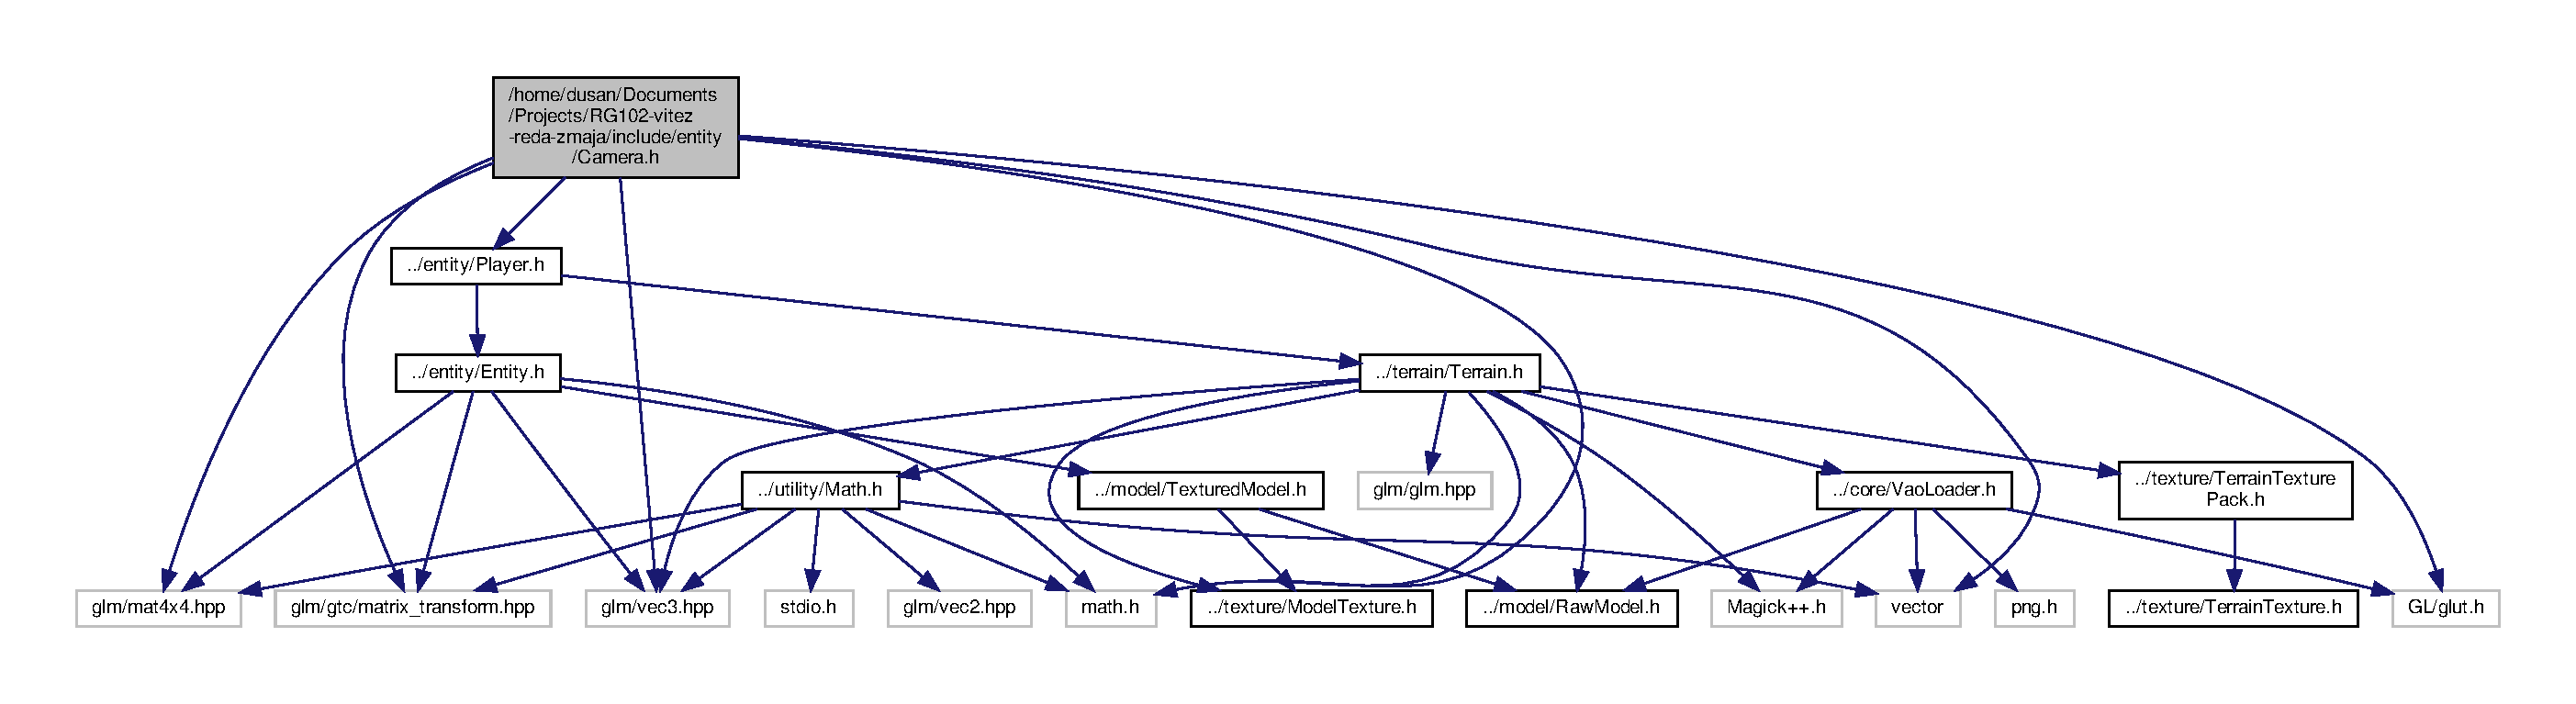
\includegraphics[width=350pt]{Camera_8h__incl}
\end{center}
\end{figure}
Ovaj graf pokazuje koje datoteke direktno ili indirektno uključuju ovu datoteku\+: \nopagebreak
\begin{figure}[H]
\begin{center}
\leavevmode
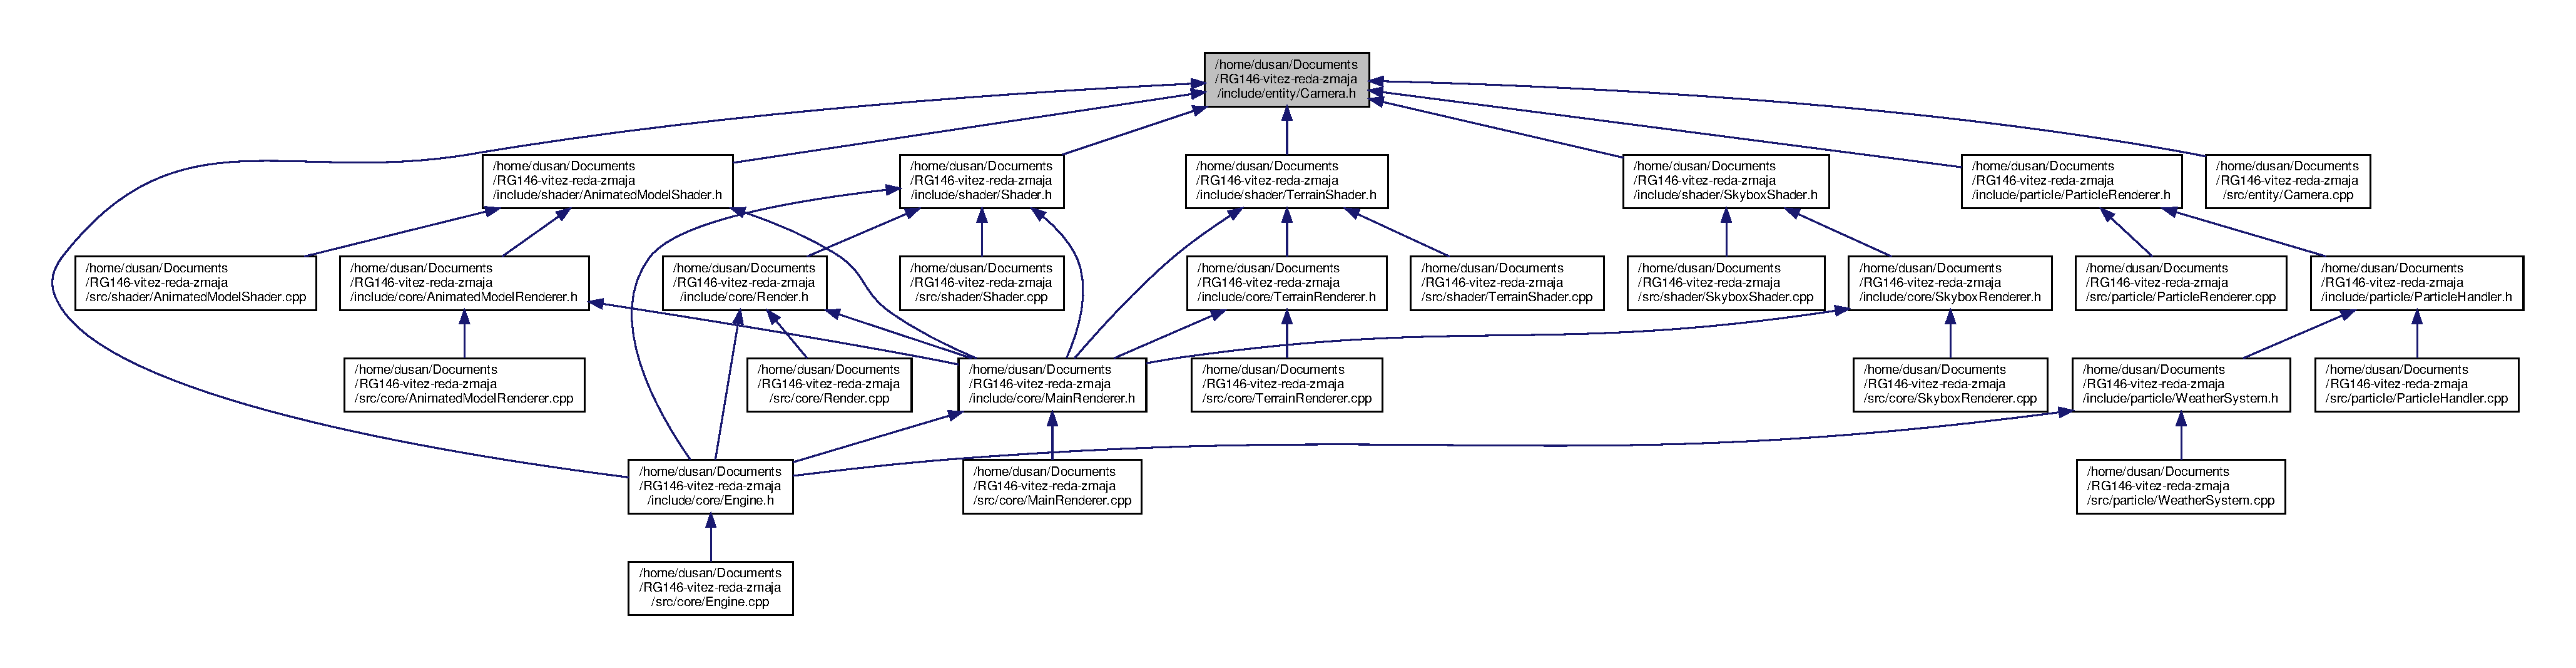
\includegraphics[width=350pt]{Camera_8h__dep__incl}
\end{center}
\end{figure}
\subsection*{Klase, strukture i unije}
\begin{DoxyCompactItemize}
\item 
class \hyperlink{classentity_1_1Camera}{entity\+::\+Camera}
\begin{DoxyCompactList}\small\item\em Klasa \hyperlink{classentity_1_1Camera}{Camera} kontrolise pogled na igru. Pomocu klase \hyperlink{classentity_1_1Camera}{Camera} mozemo menjati pogled na entitete u igri kao sto je rotiranje oko objekta i uvelicavanje ili umanjivanje. \end{DoxyCompactList}\end{DoxyCompactItemize}
\subsection*{Prostori imena}
\begin{DoxyCompactItemize}
\item 
 \hyperlink{namespaceentity}{entity}
\begin{DoxyCompactList}\small\item\em Prostor imena entity. Sadrzi sve klase, funkcije i promenljive koje odredjuju jedan entitet. \end{DoxyCompactList}\end{DoxyCompactItemize}
\subsection*{Makro zamene}
\begin{DoxyCompactItemize}
\item 
\#define \hyperlink{Camera_8h_a598a3330b3c21701223ee0ca14316eca}{PI}~3.\+14159265
\end{DoxyCompactItemize}


\subsection{Opširniji opis}
Deklaracija klase Camera. 

Deklaracija klase Camera i deklaracija callback funkcija.

\begin{DoxyAuthor}{Autor}
Dusan Pantelic 
\end{DoxyAuthor}
\begin{DoxyDate}{Datum}
Jun 2018 
\end{DoxyDate}


\subsection{Dokumentacija makro zamene}
\mbox{\Hypertarget{Camera_8h_a598a3330b3c21701223ee0ca14316eca}\label{Camera_8h_a598a3330b3c21701223ee0ca14316eca}} 
\index{Camera.\+h@{Camera.\+h}!PI@{PI}}
\index{PI@{PI}!Camera.\+h@{Camera.\+h}}
\subsubsection{\texorpdfstring{PI}{PI}}
{\footnotesize\ttfamily \#define PI~3.\+14159265}


\hypertarget{Entity_8h}{}\section{Opis datoteke /home/dusan/\+Documents/\+R\+G146-\/vitez-\/reda-\/zmaja/include/entity/\+Entity.h}
\label{Entity_8h}\index{/home/dusan/\+Documents/\+R\+G146-\/vitez-\/reda-\/zmaja/include/entity/\+Entity.\+h@{/home/dusan/\+Documents/\+R\+G146-\/vitez-\/reda-\/zmaja/include/entity/\+Entity.\+h}}


Deklaracija klase Entity.  


{\ttfamily \#include \char`\"{}../model/\+Textured\+Model.\+h\char`\"{}}\newline
{\ttfamily \#include $<$glm/vec3.\+hpp$>$}\newline
{\ttfamily \#include $<$glm/mat4x4.\+hpp$>$}\newline
{\ttfamily \#include $<$glm/gtc/matrix\+\_\+transform.\+hpp$>$}\newline
{\ttfamily \#include $<$math.\+h$>$}\newline
Graf zavisnosti datoteka za Entity.\+h\+:\nopagebreak
\begin{figure}[H]
\begin{center}
\leavevmode
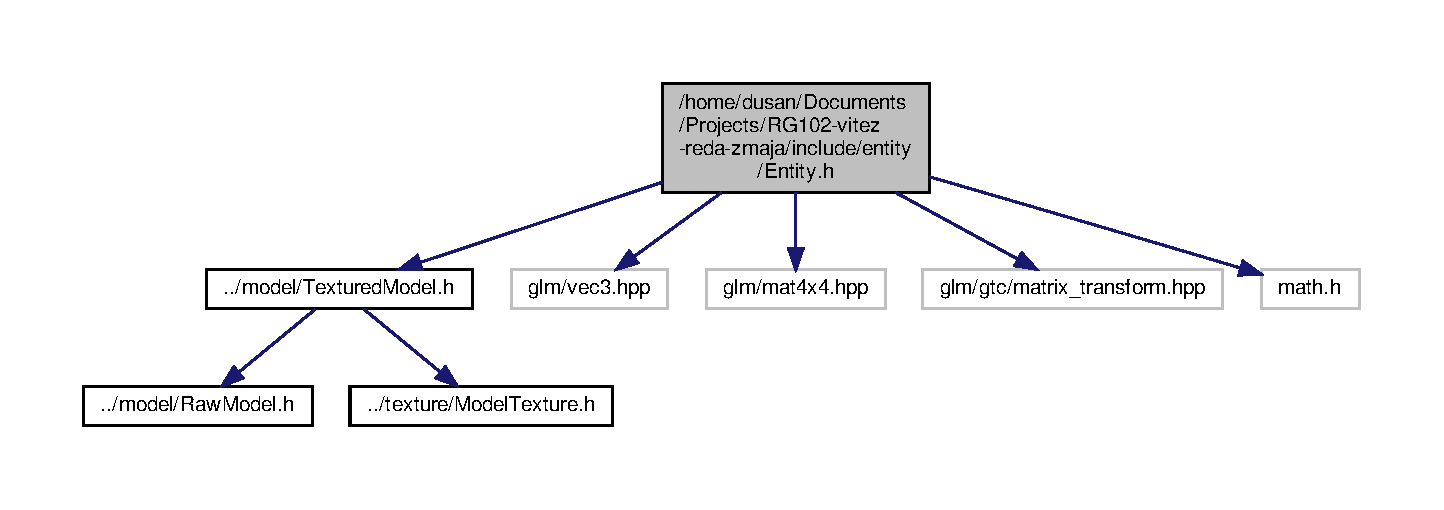
\includegraphics[width=350pt]{Entity_8h__incl}
\end{center}
\end{figure}
Ovaj graf pokazuje koje datoteke direktno ili indirektno uključuju ovu datoteku\+: \nopagebreak
\begin{figure}[H]
\begin{center}
\leavevmode
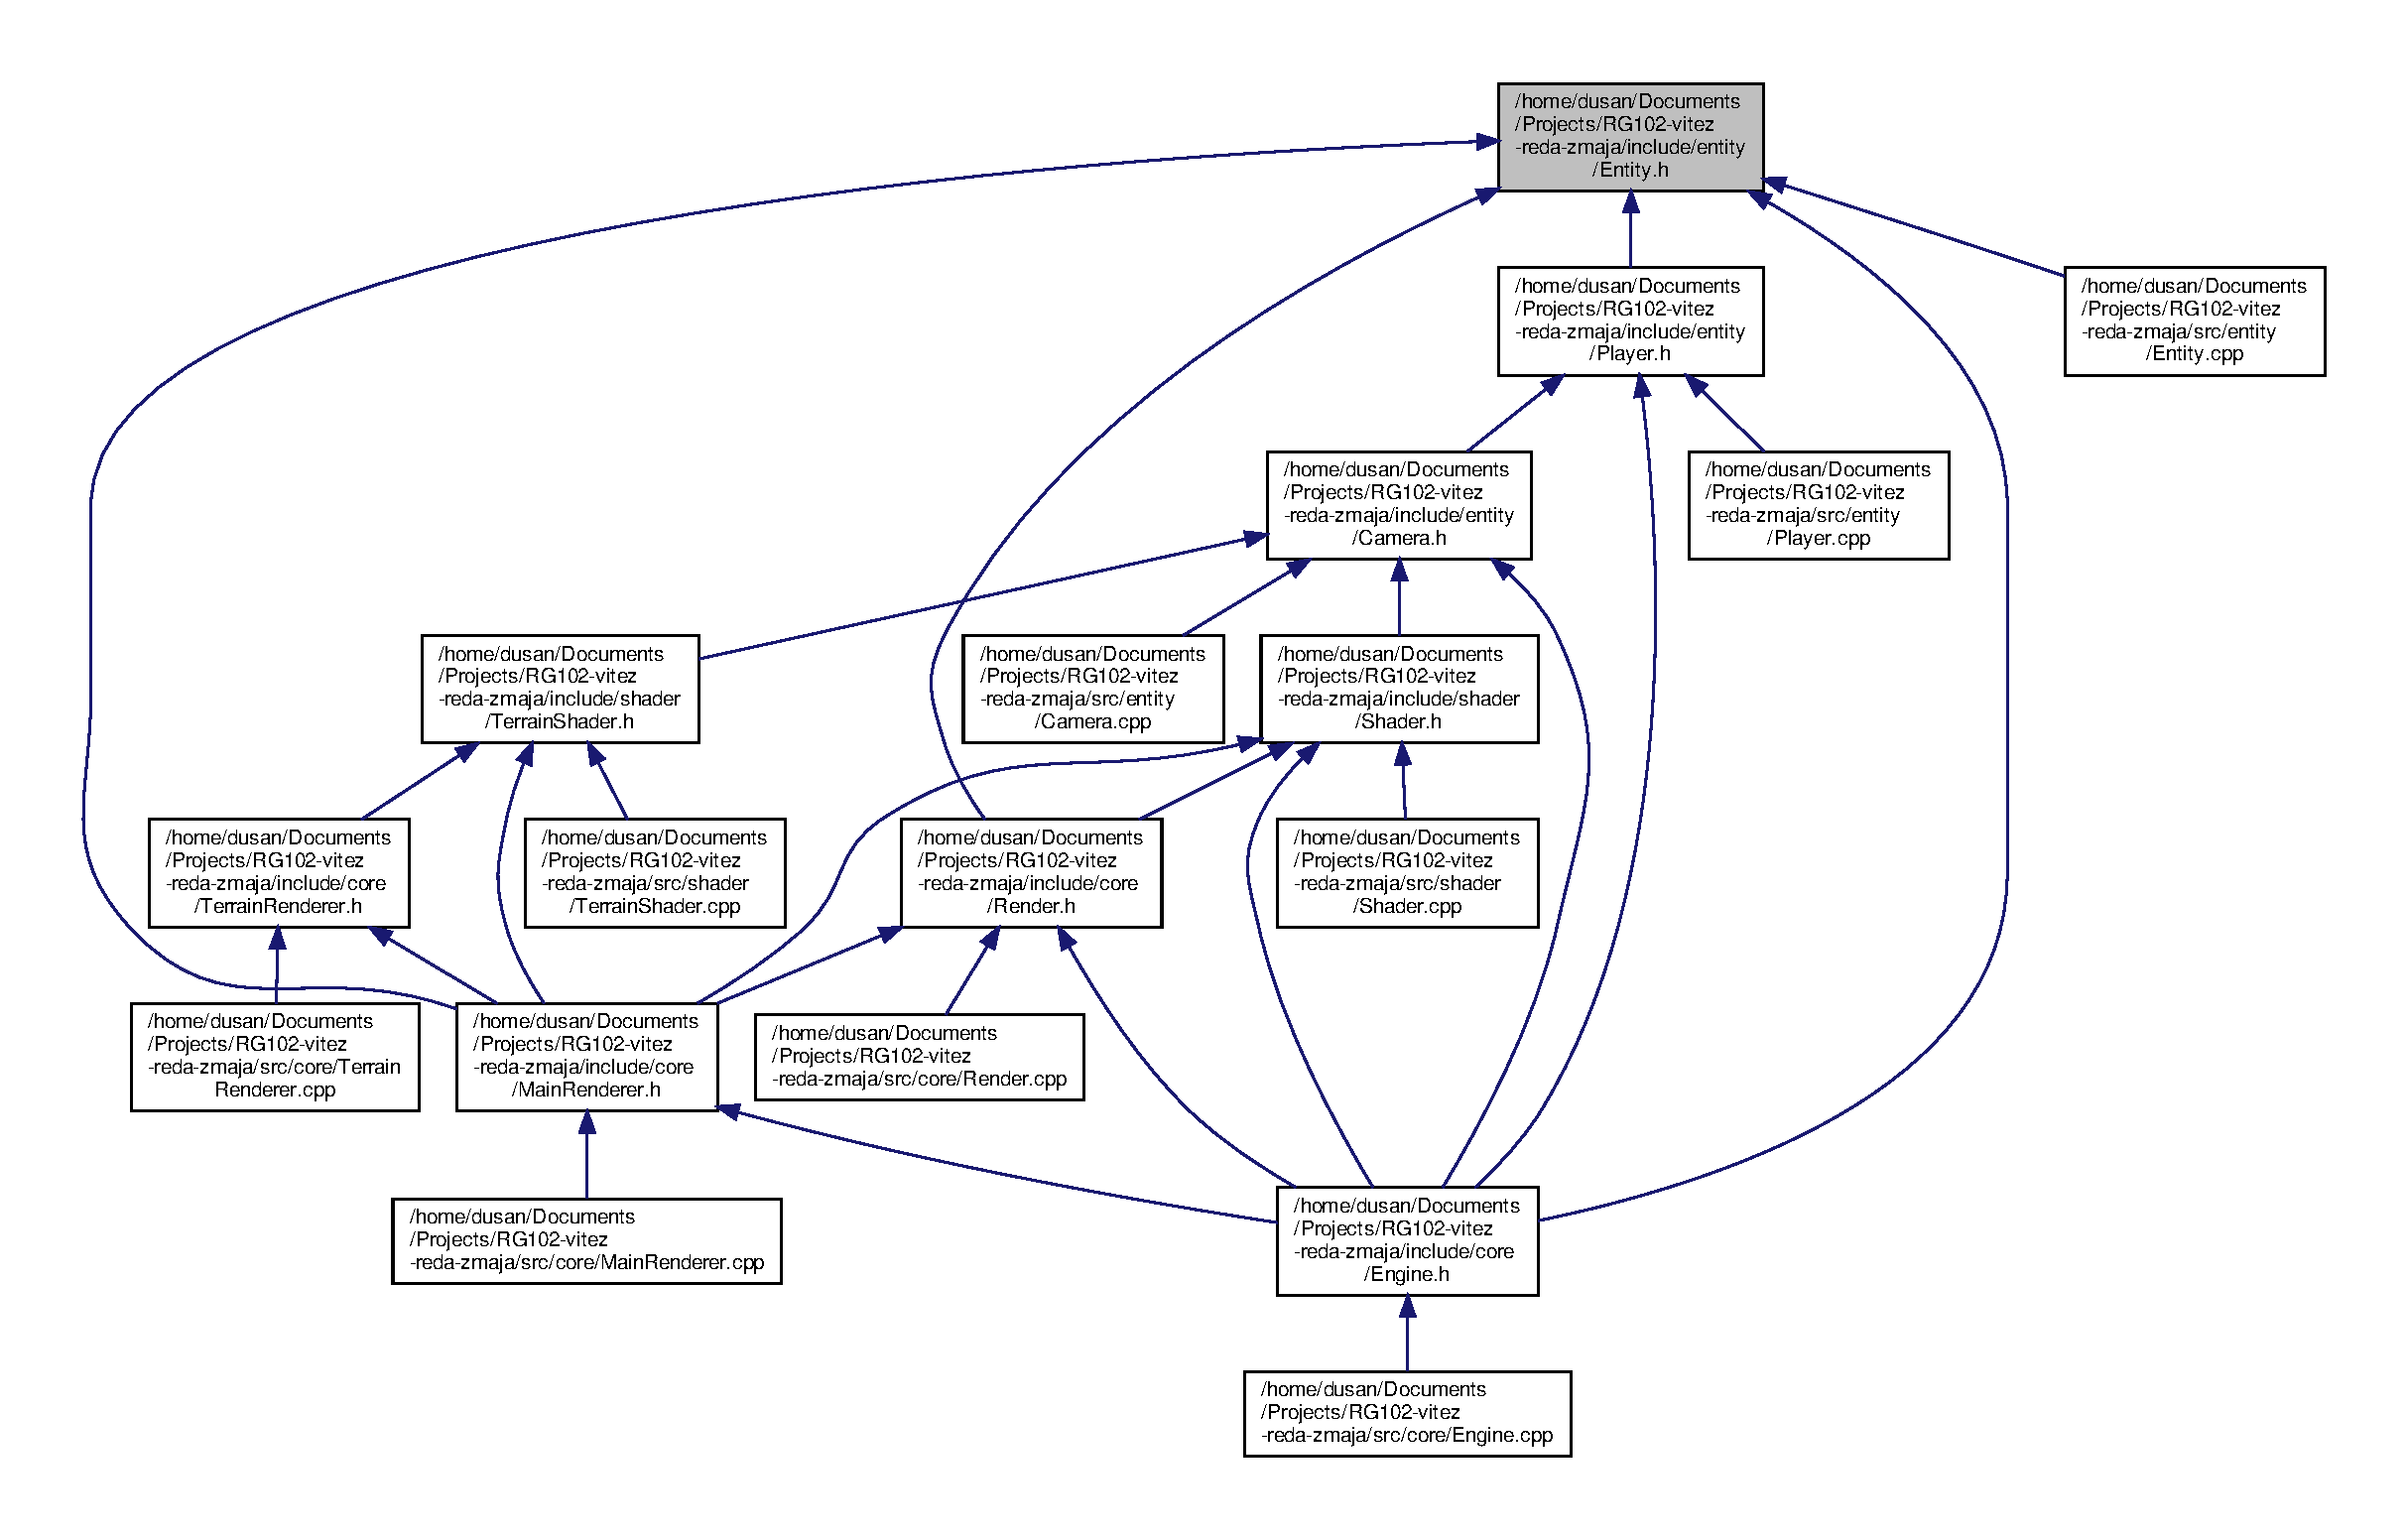
\includegraphics[width=350pt]{Entity_8h__dep__incl}
\end{center}
\end{figure}
\subsection*{Klase, strukture i unije}
\begin{DoxyCompactItemize}
\item 
class \hyperlink{classentity_1_1Entity}{entity\+::\+Entity}
\begin{DoxyCompactList}\small\item\em Klasa \hyperlink{classentity_1_1Entity}{Entity} odredjuje jedan entitet. Pomocu klase \hyperlink{classentity_1_1Entity}{Entity} odredjujemo entitet tako sto mu pridruzujemo teksturisan model kao i poziciju u svetu i ostale transformacije. \end{DoxyCompactList}\end{DoxyCompactItemize}
\subsection*{Prostori imena}
\begin{DoxyCompactItemize}
\item 
 \hyperlink{namespaceentity}{entity}
\begin{DoxyCompactList}\small\item\em Prostor imena entity. Sadrzi sve klase, funkcije i promenljive koje odredjuju jedan entitet. \end{DoxyCompactList}\end{DoxyCompactItemize}
\subsection*{Makro zamene}
\begin{DoxyCompactItemize}
\item 
\#define \hyperlink{Entity_8h_a598a3330b3c21701223ee0ca14316eca}{PI}~3.\+14159265
\end{DoxyCompactItemize}


\subsection{Opširniji opis}
Deklaracija klase Entity. 

\begin{DoxyAuthor}{Autor}
Dusan Pantelic 
\end{DoxyAuthor}
\begin{DoxyDate}{Datum}
Jun 2018 
\end{DoxyDate}


\subsection{Dokumentacija makro zamene}
\mbox{\Hypertarget{Entity_8h_a598a3330b3c21701223ee0ca14316eca}\label{Entity_8h_a598a3330b3c21701223ee0ca14316eca}} 
\index{Entity.\+h@{Entity.\+h}!PI@{PI}}
\index{PI@{PI}!Entity.\+h@{Entity.\+h}}
\subsubsection{\texorpdfstring{PI}{PI}}
{\footnotesize\ttfamily \#define PI~3.\+14159265}


\hypertarget{Light_8h}{}\section{Opis datoteke /home/dusan/\+Documents/\+Projects/\+R\+G102-\/vitez-\/reda-\/zmaja/include/entity/\+Light.h}
\label{Light_8h}\index{/home/dusan/\+Documents/\+Projects/\+R\+G102-\/vitez-\/reda-\/zmaja/include/entity/\+Light.\+h@{/home/dusan/\+Documents/\+Projects/\+R\+G102-\/vitez-\/reda-\/zmaja/include/entity/\+Light.\+h}}
{\ttfamily \#include $<$glm/vec3.\+hpp$>$}\newline
{\ttfamily \#include $<$glm/mat4x4.\+hpp$>$}\newline
{\ttfamily \#include $<$glm/gtc/matrix\+\_\+transform.\+hpp$>$}\newline
Graf zavisnosti datoteka za Light.\+h\+:
\nopagebreak
\begin{figure}[H]
\begin{center}
\leavevmode
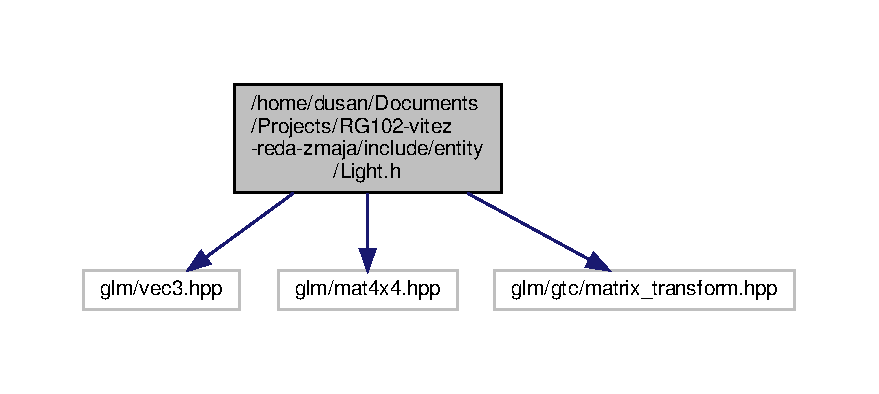
\includegraphics[width=350pt]{Light_8h__incl}
\end{center}
\end{figure}
Ovaj graf pokazuje koje datoteke direktno ili indirektno uključuju ovu datoteku\+: 
\nopagebreak
\begin{figure}[H]
\begin{center}
\leavevmode
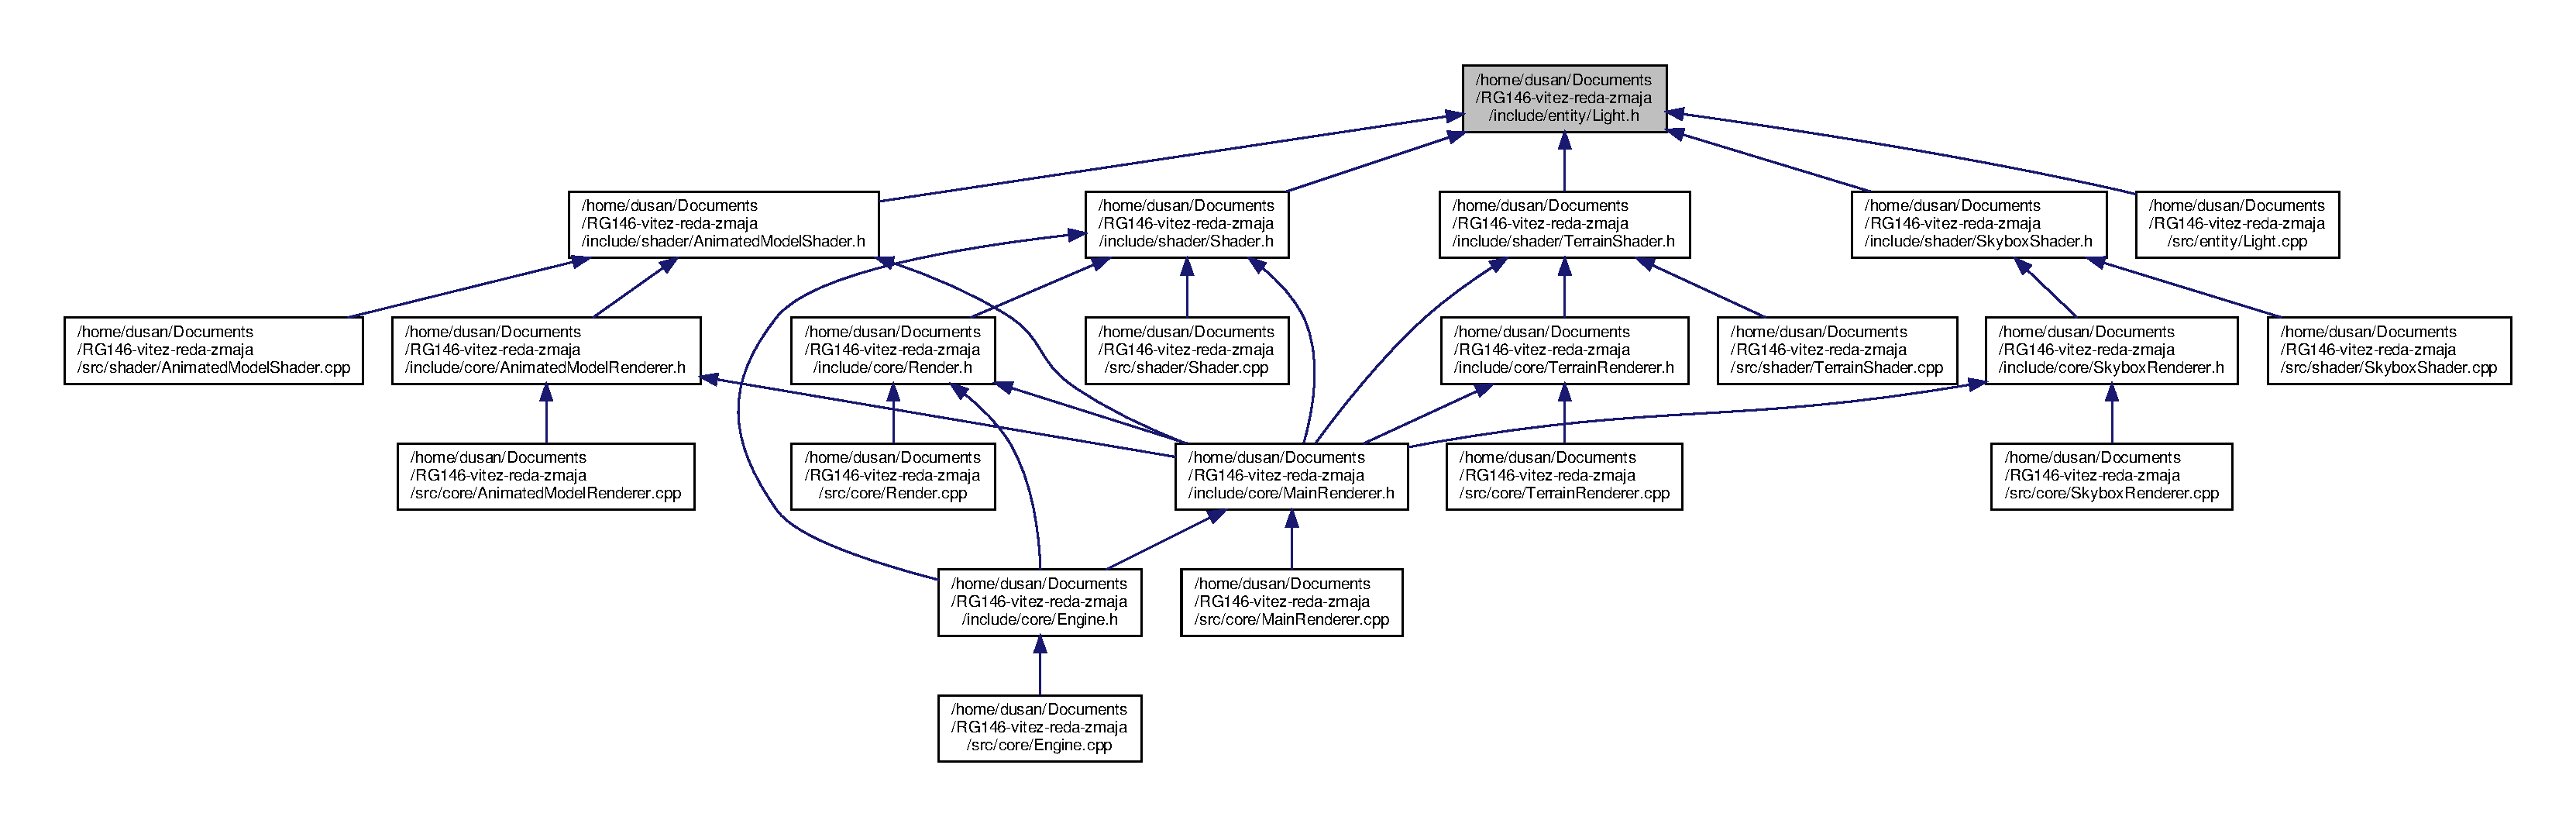
\includegraphics[width=350pt]{Light_8h__dep__incl}
\end{center}
\end{figure}
\subsection*{Klase, strukture i unije}
\begin{DoxyCompactItemize}
\item 
class \hyperlink{classentity_1_1Light}{entity\+::\+Light}
\begin{DoxyCompactList}\small\item\em Klasa \hyperlink{classentity_1_1Light}{Light} odredjuje osvetljenost. Pomocu klase \hyperlink{classentity_1_1Light}{Light} odredjujemo poziciju boju kao i intenzitet svetlosti. \end{DoxyCompactList}\end{DoxyCompactItemize}
\subsection*{Prostori imena}
\begin{DoxyCompactItemize}
\item 
 \hyperlink{namespaceentity}{entity}
\begin{DoxyCompactList}\small\item\em Prostor imena entity. Sadrzi sve klase, funkcije i promenljive koje odredjuju jedan entitet. \end{DoxyCompactList}\end{DoxyCompactItemize}

\hypertarget{Player_8h}{}\section{Opis datoteke /home/dusan/\+Documents/\+R\+G146-\/vitez-\/reda-\/zmaja/include/entity/\+Player.h}
\label{Player_8h}\index{/home/dusan/\+Documents/\+R\+G146-\/vitez-\/reda-\/zmaja/include/entity/\+Player.\+h@{/home/dusan/\+Documents/\+R\+G146-\/vitez-\/reda-\/zmaja/include/entity/\+Player.\+h}}


Deklaracija klase Player.  


{\ttfamily \#include \char`\"{}../entity/\+Animated\+Entity.\+h\char`\"{}}\newline
{\ttfamily \#include \char`\"{}../terrain/\+Terrain.\+h\char`\"{}}\newline
{\ttfamily \#include \char`\"{}../utility/\+Fps\+Data.\+h\char`\"{}}\newline
{\ttfamily \#include \char`\"{}../animation/\+Animator.\+h\char`\"{}}\newline
Graf zavisnosti datoteka za Player.\+h\+:
\nopagebreak
\begin{figure}[H]
\begin{center}
\leavevmode
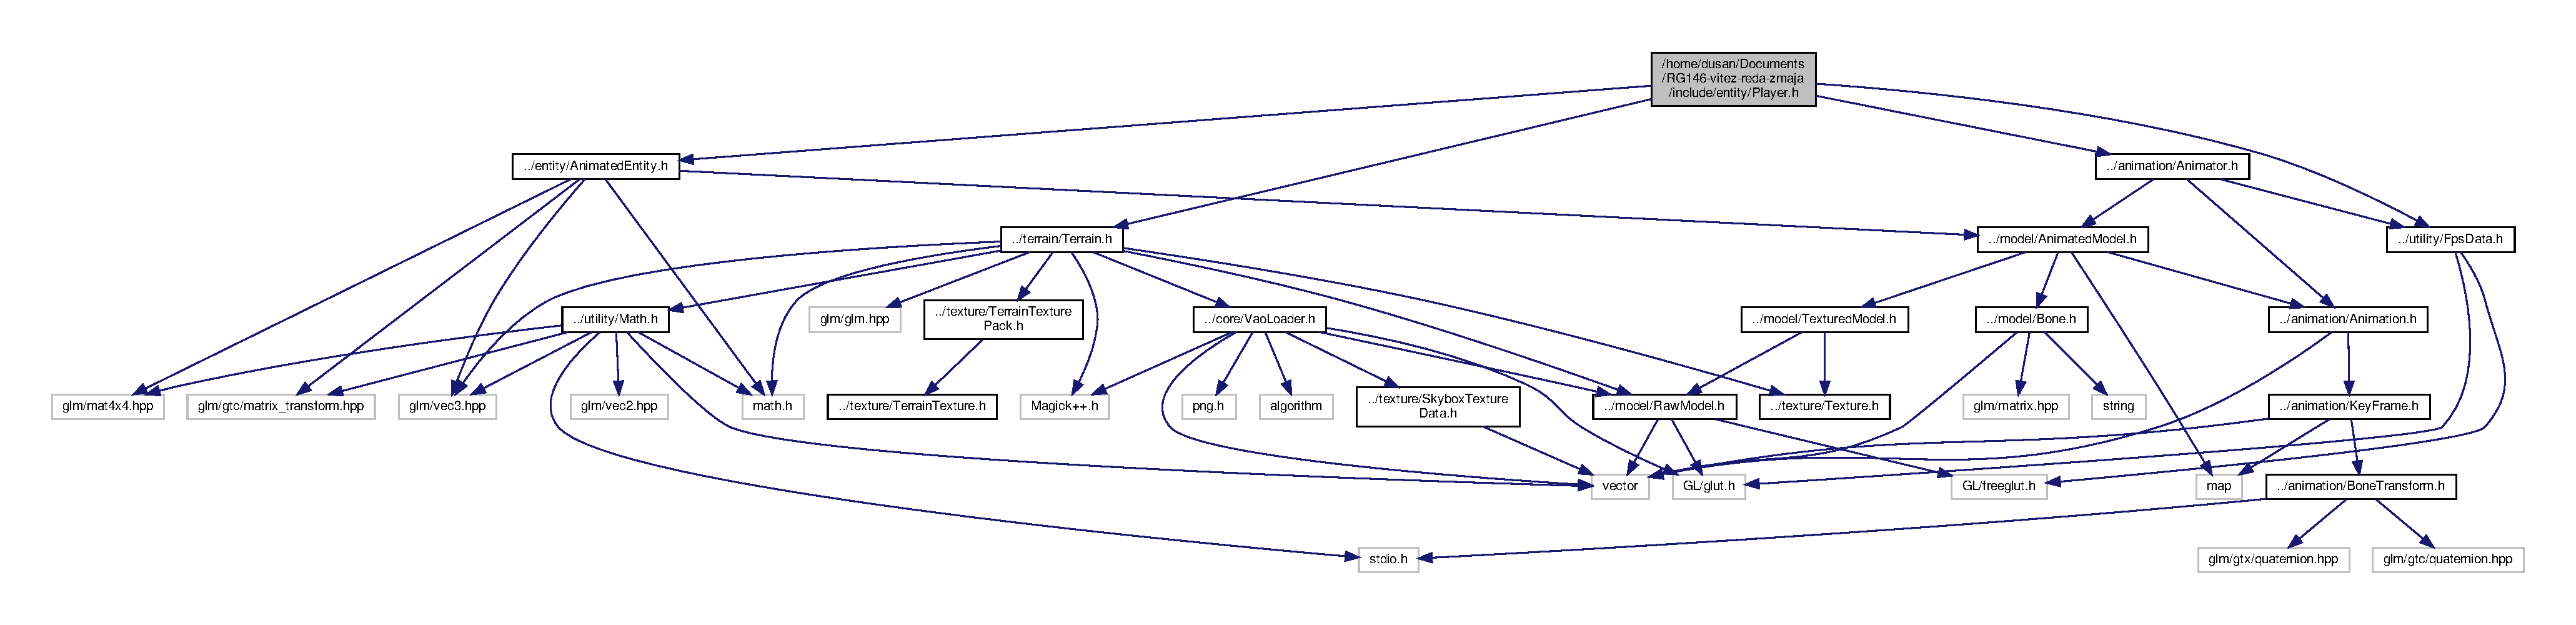
\includegraphics[width=350pt]{Player_8h__incl}
\end{center}
\end{figure}
Ovaj graf pokazuje koje datoteke direktno ili indirektno uključuju ovu datoteku\+: 
\nopagebreak
\begin{figure}[H]
\begin{center}
\leavevmode
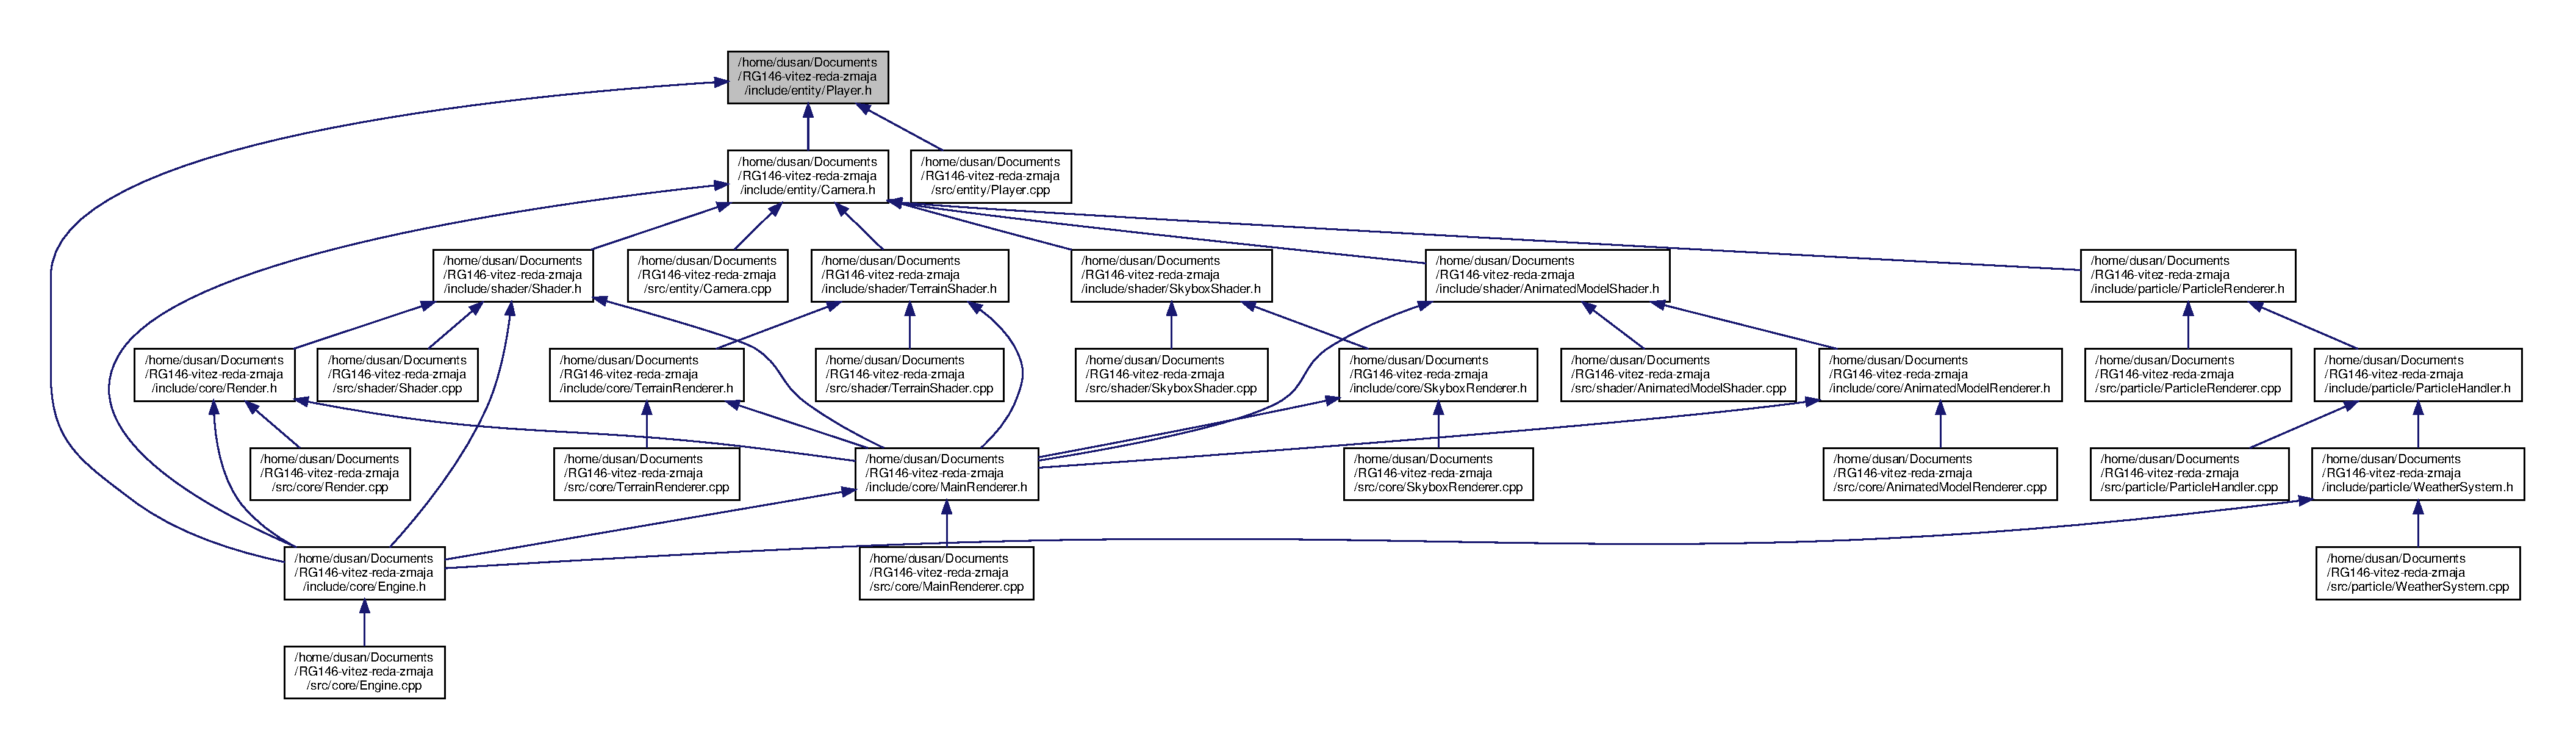
\includegraphics[width=350pt]{Player_8h__dep__incl}
\end{center}
\end{figure}
\subsection*{Klase, strukture i unije}
\begin{DoxyCompactItemize}
\item 
class \hyperlink{classentity_1_1Player}{entity\+::\+Player}
\begin{DoxyCompactList}\small\item\em Klasa \hyperlink{classentity_1_1Player}{Player} odredjuje igraca koji nadogradjuje entitet. Pomocu klase \hyperlink{classentity_1_1Player}{Player} nadogradjujemo klasu \hyperlink{classentity_1_1Entity}{Entity} dodavajuci jos nove atribute i funkcije. \end{DoxyCompactList}\end{DoxyCompactItemize}
\subsection*{Prostori imena}
\begin{DoxyCompactItemize}
\item 
 \hyperlink{namespaceentity}{entity}
\begin{DoxyCompactList}\small\item\em Prostor imena entity. Sadrzi sve klase, funkcije i promenljive koje odredjuju jedan entitet. \end{DoxyCompactList}\end{DoxyCompactItemize}
\subsection*{Makro zamene}
\begin{DoxyCompactItemize}
\item 
\#define \hyperlink{Player_8h_aa5f3efb32c476acce65037d89e154c60}{R\+U\+N\+\_\+\+S\+P\+E\+ED}~10
\item 
\#define \hyperlink{Player_8h_afa9188776d909e94ead6cf6ffbbdd1e8}{T\+U\+R\+N\+\_\+\+S\+P\+E\+ED}~50
\end{DoxyCompactItemize}


\subsection{Opširniji opis}
Deklaracija klase Player. 

\begin{DoxyAuthor}{Autor}
Dusan Pantelic 
\end{DoxyAuthor}
\begin{DoxyDate}{Datum}
Septembar 2018 
\end{DoxyDate}


\subsection{Dokumentacija makro zamene}
\mbox{\Hypertarget{Player_8h_aa5f3efb32c476acce65037d89e154c60}\label{Player_8h_aa5f3efb32c476acce65037d89e154c60}} 
\index{Player.\+h@{Player.\+h}!R\+U\+N\+\_\+\+S\+P\+E\+ED@{R\+U\+N\+\_\+\+S\+P\+E\+ED}}
\index{R\+U\+N\+\_\+\+S\+P\+E\+ED@{R\+U\+N\+\_\+\+S\+P\+E\+ED}!Player.\+h@{Player.\+h}}
\subsubsection{\texorpdfstring{R\+U\+N\+\_\+\+S\+P\+E\+ED}{RUN\_SPEED}}
{\footnotesize\ttfamily \#define R\+U\+N\+\_\+\+S\+P\+E\+ED~10}

\mbox{\Hypertarget{Player_8h_afa9188776d909e94ead6cf6ffbbdd1e8}\label{Player_8h_afa9188776d909e94ead6cf6ffbbdd1e8}} 
\index{Player.\+h@{Player.\+h}!T\+U\+R\+N\+\_\+\+S\+P\+E\+ED@{T\+U\+R\+N\+\_\+\+S\+P\+E\+ED}}
\index{T\+U\+R\+N\+\_\+\+S\+P\+E\+ED@{T\+U\+R\+N\+\_\+\+S\+P\+E\+ED}!Player.\+h@{Player.\+h}}
\subsubsection{\texorpdfstring{T\+U\+R\+N\+\_\+\+S\+P\+E\+ED}{TURN\_SPEED}}
{\footnotesize\ttfamily \#define T\+U\+R\+N\+\_\+\+S\+P\+E\+ED~50}


\hypertarget{tiny__obj__loader_8h}{}\section{Opis datoteke /home/dusan/\+Documents/\+Projects/\+R\+G102-\/vitez-\/reda-\/zmaja/include/external\+\_\+libs/tiny\+\_\+obj\+\_\+loader.h}
\label{tiny__obj__loader_8h}\index{/home/dusan/\+Documents/\+Projects/\+R\+G102-\/vitez-\/reda-\/zmaja/include/external\+\_\+libs/tiny\+\_\+obj\+\_\+loader.\+h@{/home/dusan/\+Documents/\+Projects/\+R\+G102-\/vitez-\/reda-\/zmaja/include/external\+\_\+libs/tiny\+\_\+obj\+\_\+loader.\+h}}
{\ttfamily \#include $<$map$>$}\newline
{\ttfamily \#include $<$string$>$}\newline
{\ttfamily \#include $<$vector$>$}\newline
{\ttfamily \#include $<$cassert$>$}\newline
{\ttfamily \#include $<$cctype$>$}\newline
{\ttfamily \#include $<$cmath$>$}\newline
{\ttfamily \#include $<$cstddef$>$}\newline
{\ttfamily \#include $<$cstdlib$>$}\newline
{\ttfamily \#include $<$cstring$>$}\newline
{\ttfamily \#include $<$limits$>$}\newline
{\ttfamily \#include $<$utility$>$}\newline
{\ttfamily \#include $<$fstream$>$}\newline
{\ttfamily \#include $<$sstream$>$}\newline
Graf zavisnosti datoteka za tiny\+\_\+obj\+\_\+loader.\+h\+:
\nopagebreak
\begin{figure}[H]
\begin{center}
\leavevmode
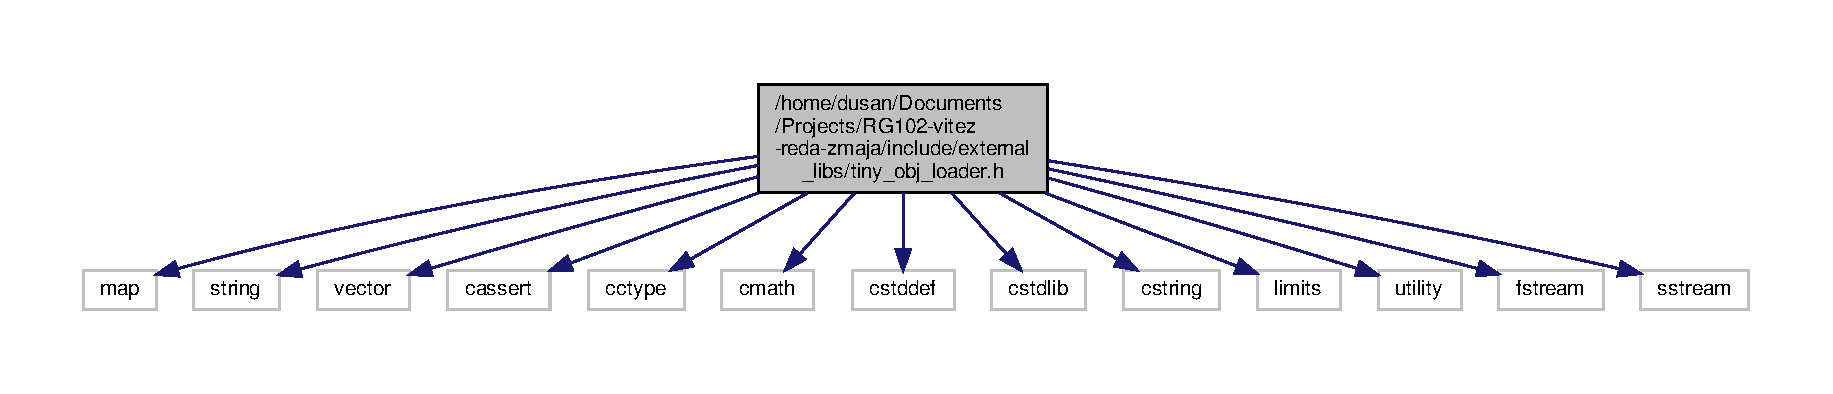
\includegraphics[width=350pt]{tiny__obj__loader_8h__incl}
\end{center}
\end{figure}
Ovaj graf pokazuje koje datoteke direktno ili indirektno uključuju ovu datoteku\+: 
\nopagebreak
\begin{figure}[H]
\begin{center}
\leavevmode
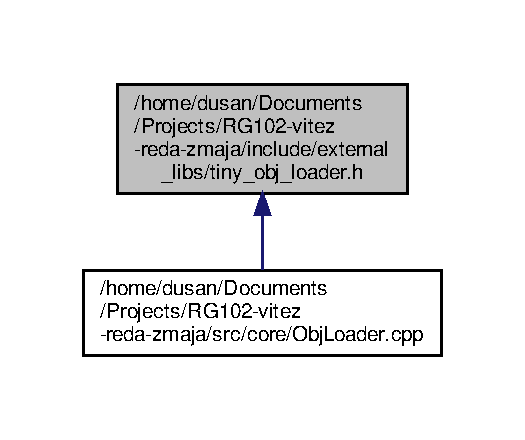
\includegraphics[width=252pt]{tiny__obj__loader_8h__dep__incl}
\end{center}
\end{figure}
\subsection*{Klase, strukture i unije}
\begin{DoxyCompactItemize}
\item 
struct \hyperlink{structtinyobj_1_1texture__option__t}{tinyobj\+::texture\+\_\+option\+\_\+t}
\item 
struct \hyperlink{structtinyobj_1_1material__t}{tinyobj\+::material\+\_\+t}
\item 
struct \hyperlink{structtinyobj_1_1tag__t}{tinyobj\+::tag\+\_\+t}
\item 
struct \hyperlink{structtinyobj_1_1index__t}{tinyobj\+::index\+\_\+t}
\item 
struct \hyperlink{structtinyobj_1_1mesh__t}{tinyobj\+::mesh\+\_\+t}
\item 
struct \hyperlink{structtinyobj_1_1path__t}{tinyobj\+::path\+\_\+t}
\item 
struct \hyperlink{structtinyobj_1_1shape__t}{tinyobj\+::shape\+\_\+t}
\item 
struct \hyperlink{structtinyobj_1_1attrib__t}{tinyobj\+::attrib\+\_\+t}
\item 
struct \hyperlink{structtinyobj_1_1callback__t__}{tinyobj\+::callback\+\_\+t\+\_\+}
\item 
class \hyperlink{classtinyobj_1_1MaterialReader}{tinyobj\+::\+Material\+Reader}
\item 
class \hyperlink{classtinyobj_1_1MaterialFileReader}{tinyobj\+::\+Material\+File\+Reader}
\item 
class \hyperlink{classtinyobj_1_1MaterialStreamReader}{tinyobj\+::\+Material\+Stream\+Reader}
\end{DoxyCompactItemize}
\subsection*{Prostori imena}
\begin{DoxyCompactItemize}
\item 
 \hyperlink{namespacetinyobj}{tinyobj}
\end{DoxyCompactItemize}
\subsection*{Definicije tipa}
\begin{DoxyCompactItemize}
\item 
typedef float \hyperlink{namespacetinyobj_ad5ca7469ff56bf0d8423120cfd99adce}{tinyobj\+::real\+\_\+t}
\item 
typedef struct \hyperlink{structtinyobj_1_1callback__t__}{tinyobj\+::callback\+\_\+t\+\_\+} \hyperlink{namespacetinyobj_a7d9ae2b4716367a1b66b4d354482b035}{tinyobj\+::callback\+\_\+t}
\end{DoxyCompactItemize}
\subsection*{Nabrajanja}
\begin{DoxyCompactItemize}
\item 
enum \hyperlink{namespacetinyobj_a5c9f207e1f880a48bac0a3b69f16d7f8}{tinyobj\+::texture\+\_\+type\+\_\+t} \{ \newline
\hyperlink{namespacetinyobj_a5c9f207e1f880a48bac0a3b69f16d7f8a259804f2e7bf9c39626abe6ebce6edc1}{tinyobj\+::\+T\+E\+X\+T\+U\+R\+E\+\_\+\+T\+Y\+P\+E\+\_\+\+N\+O\+NE}, 
\hyperlink{namespacetinyobj_a5c9f207e1f880a48bac0a3b69f16d7f8a4e5a6bfb8a95a23bf0cce576aaa5dfa4}{tinyobj\+::\+T\+E\+X\+T\+U\+R\+E\+\_\+\+T\+Y\+P\+E\+\_\+\+S\+P\+H\+E\+RE}, 
\hyperlink{namespacetinyobj_a5c9f207e1f880a48bac0a3b69f16d7f8acc4c4327df32dce3fa406865a8e35519}{tinyobj\+::\+T\+E\+X\+T\+U\+R\+E\+\_\+\+T\+Y\+P\+E\+\_\+\+C\+U\+B\+E\+\_\+\+T\+OP}, 
\hyperlink{namespacetinyobj_a5c9f207e1f880a48bac0a3b69f16d7f8a20c37be3992ed111ba47045a63351cde}{tinyobj\+::\+T\+E\+X\+T\+U\+R\+E\+\_\+\+T\+Y\+P\+E\+\_\+\+C\+U\+B\+E\+\_\+\+B\+O\+T\+T\+OM}, 
\newline
\hyperlink{namespacetinyobj_a5c9f207e1f880a48bac0a3b69f16d7f8a1ce5bed3c2ba5c360ca6c2607b9d97ca}{tinyobj\+::\+T\+E\+X\+T\+U\+R\+E\+\_\+\+T\+Y\+P\+E\+\_\+\+C\+U\+B\+E\+\_\+\+F\+R\+O\+NT}, 
\hyperlink{namespacetinyobj_a5c9f207e1f880a48bac0a3b69f16d7f8af2cb2d4e7551e713593382c4690aa665}{tinyobj\+::\+T\+E\+X\+T\+U\+R\+E\+\_\+\+T\+Y\+P\+E\+\_\+\+C\+U\+B\+E\+\_\+\+B\+A\+CK}, 
\hyperlink{namespacetinyobj_a5c9f207e1f880a48bac0a3b69f16d7f8a01f908bcfb745ad0d97d84b8cacc6d30}{tinyobj\+::\+T\+E\+X\+T\+U\+R\+E\+\_\+\+T\+Y\+P\+E\+\_\+\+C\+U\+B\+E\+\_\+\+L\+E\+FT}, 
\hyperlink{namespacetinyobj_a5c9f207e1f880a48bac0a3b69f16d7f8a7709b5986f04e87ffbdc9bd7280d261c}{tinyobj\+::\+T\+E\+X\+T\+U\+R\+E\+\_\+\+T\+Y\+P\+E\+\_\+\+C\+U\+B\+E\+\_\+\+R\+I\+G\+HT}
 \}
\end{DoxyCompactItemize}
\subsection*{Funkcije}
\begin{DoxyCompactItemize}
\item 
bool \hyperlink{namespacetinyobj_a5678f6df6cb6d01bb89453022d997503}{tinyobj\+::\+Load\+Obj} (attrib\+\_\+t $\ast$attrib, std\+::vector$<$ shape\+\_\+t $>$ $\ast$shapes, std\+::vector$<$ material\+\_\+t $>$ $\ast$materials, std\+::string $\ast$err, const char $\ast$filename, const char $\ast$mtl\+\_\+basedir=N\+U\+LL, bool triangulate=true)
\item 
bool \hyperlink{namespacetinyobj_add9ad979e8011ccdfac2e1ec8def5359}{tinyobj\+::\+Load\+Obj\+With\+Callback} (std\+::istream \&in\+Stream, const callback\+\_\+t \&callback, void $\ast$user\+\_\+data=N\+U\+LL, Material\+Reader $\ast$read\+Mat\+Fn=N\+U\+LL, std\+::string $\ast$err=N\+U\+LL)
\item 
bool \hyperlink{namespacetinyobj_ad1e942879313375fcd1b08b7d6e7f89d}{tinyobj\+::\+Load\+Obj} (attrib\+\_\+t $\ast$attrib, std\+::vector$<$ shape\+\_\+t $>$ $\ast$shapes, std\+::vector$<$ material\+\_\+t $>$ $\ast$materials, std\+::string $\ast$err, std\+::istream $\ast$in\+Stream, Material\+Reader $\ast$read\+Mat\+Fn=N\+U\+LL, bool triangulate=true)
\item 
void \hyperlink{namespacetinyobj_aa7a035d152857396e5cde8ebff8b2b9e}{tinyobj\+::\+Load\+Mtl} (std\+::map$<$ std\+::string, int $>$ $\ast$material\+\_\+map, std\+::vector$<$ material\+\_\+t $>$ $\ast$materials, std\+::istream $\ast$in\+Stream, std\+::string $\ast$warning)
\begin{DoxyCompactList}\small\item\em Loads materials into std\+::map. \end{DoxyCompactList}\end{DoxyCompactItemize}

\hypertarget{RawModel_8h}{}\section{Opis datoteke /home/dusan/\+Documents/\+R\+G146-\/vitez-\/reda-\/zmaja/include/model/\+Raw\+Model.h}
\label{RawModel_8h}\index{/home/dusan/\+Documents/\+R\+G146-\/vitez-\/reda-\/zmaja/include/model/\+Raw\+Model.\+h@{/home/dusan/\+Documents/\+R\+G146-\/vitez-\/reda-\/zmaja/include/model/\+Raw\+Model.\+h}}


Deklaracija klase Raw\+Model.  


Ovaj graf pokazuje koje datoteke direktno ili indirektno uključuju ovu datoteku\+: \nopagebreak
\begin{figure}[H]
\begin{center}
\leavevmode
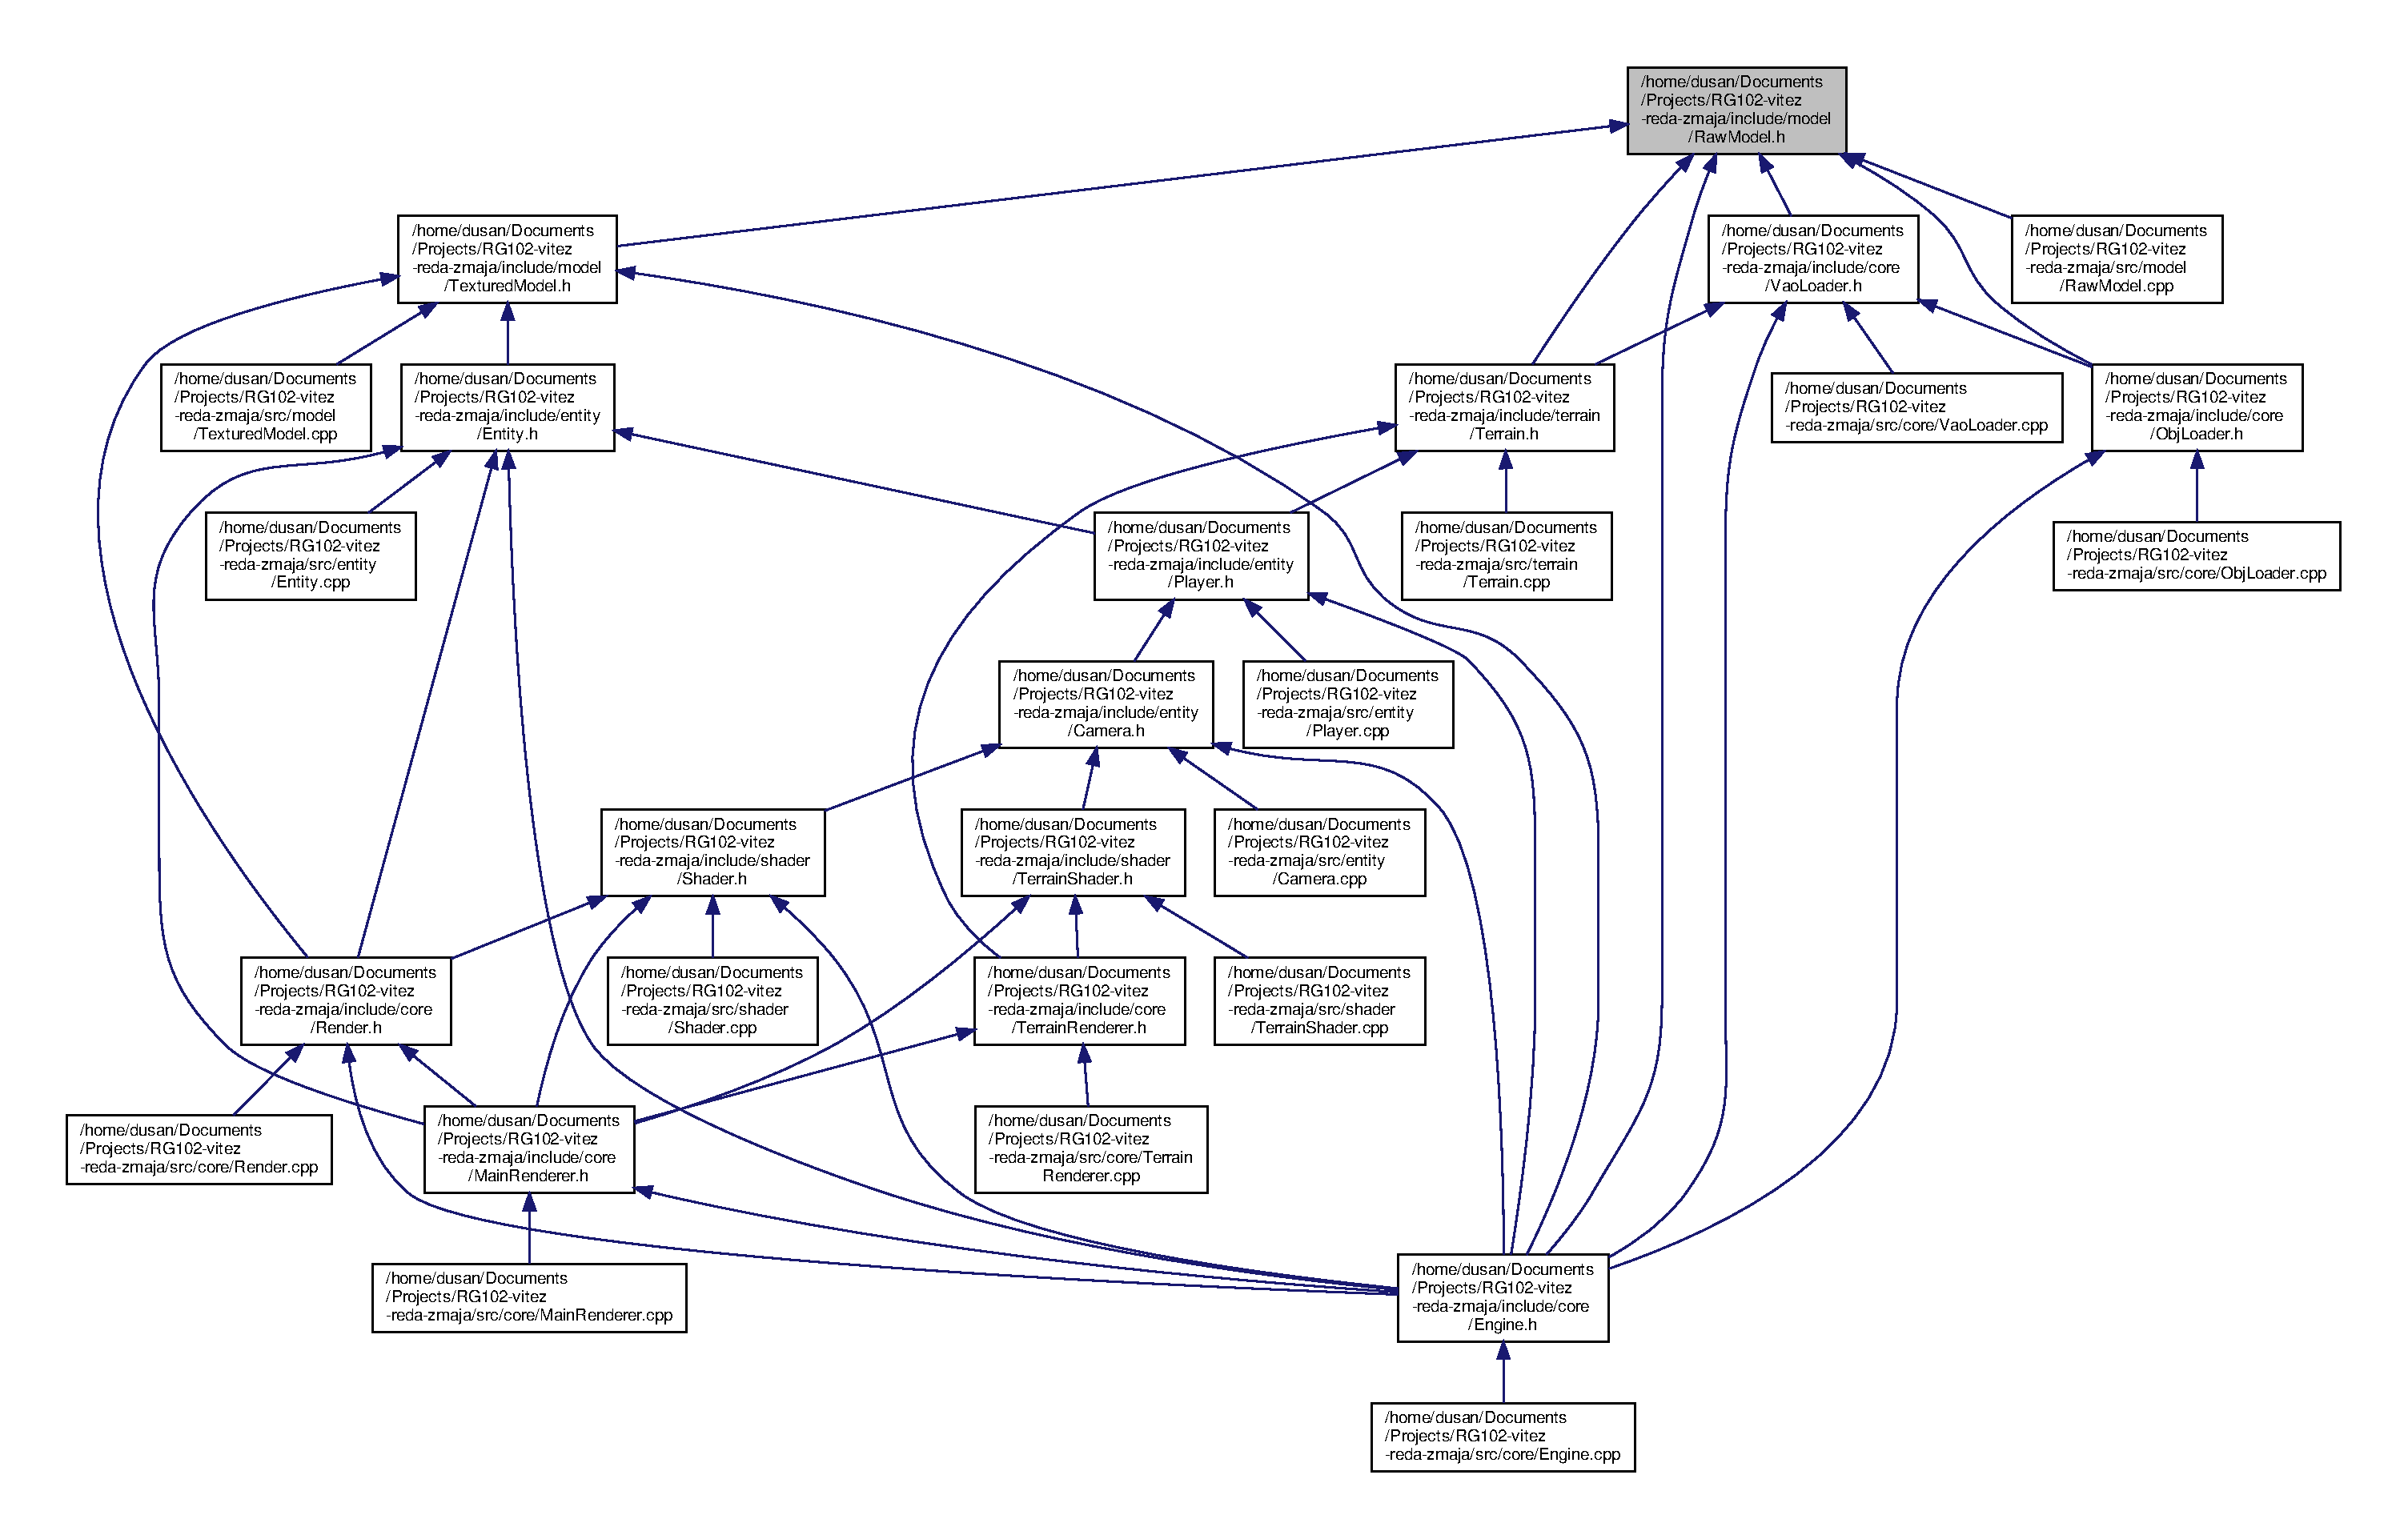
\includegraphics[width=350pt]{RawModel_8h__dep__incl}
\end{center}
\end{figure}
\subsection*{Klase, strukture i unije}
\begin{DoxyCompactItemize}
\item 
class \hyperlink{classmodel_1_1RawModel}{model\+::\+Raw\+Model}
\begin{DoxyCompactList}\small\item\em Klasa \hyperlink{classmodel_1_1RawModel}{Raw\+Model} opisuje model objekta. Model je opisan brojem tacaka i pridruzenom nizu atributa. \end{DoxyCompactList}\end{DoxyCompactItemize}
\subsection*{Prostori imena}
\begin{DoxyCompactItemize}
\item 
 \hyperlink{namespacemodel}{model}
\begin{DoxyCompactList}\small\item\em Prostor imena model. Sadrzi sve klase, funkcije i promenljive koje opisuju model objekta. \end{DoxyCompactList}\end{DoxyCompactItemize}


\subsection{Opširniji opis}
Deklaracija klase Raw\+Model. 

\begin{DoxyAuthor}{Autor}
Dusan Pantelic 
\end{DoxyAuthor}
\begin{DoxyDate}{Datum}
Decembar 2017 
\end{DoxyDate}

\hypertarget{TexturedModel_8h}{}\section{Opis datoteke /home/dusan/\+Documents/\+R\+G146-\/vitez-\/reda-\/zmaja/include/model/\+Textured\+Model.h}
\label{TexturedModel_8h}\index{/home/dusan/\+Documents/\+R\+G146-\/vitez-\/reda-\/zmaja/include/model/\+Textured\+Model.\+h@{/home/dusan/\+Documents/\+R\+G146-\/vitez-\/reda-\/zmaja/include/model/\+Textured\+Model.\+h}}


Deklaracija klase Textured\+Model.  


{\ttfamily \#include \char`\"{}../model/\+Raw\+Model.\+h\char`\"{}}\newline
{\ttfamily \#include \char`\"{}../texture/\+Texture.\+h\char`\"{}}\newline
Graf zavisnosti datoteka za Textured\+Model.\+h\+:
\nopagebreak
\begin{figure}[H]
\begin{center}
\leavevmode
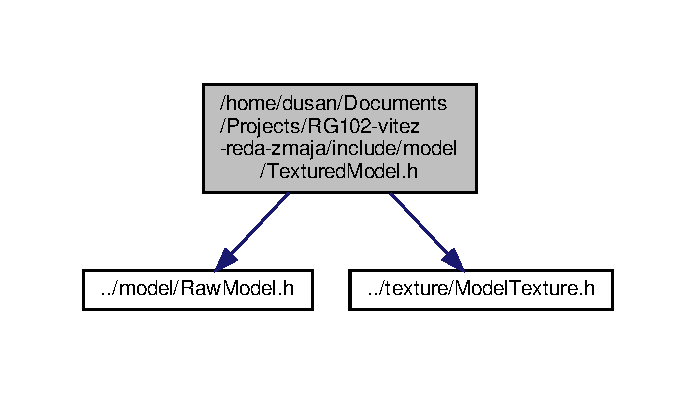
\includegraphics[width=350pt]{TexturedModel_8h__incl}
\end{center}
\end{figure}
Ovaj graf pokazuje koje datoteke direktno ili indirektno uključuju ovu datoteku\+: 
\nopagebreak
\begin{figure}[H]
\begin{center}
\leavevmode
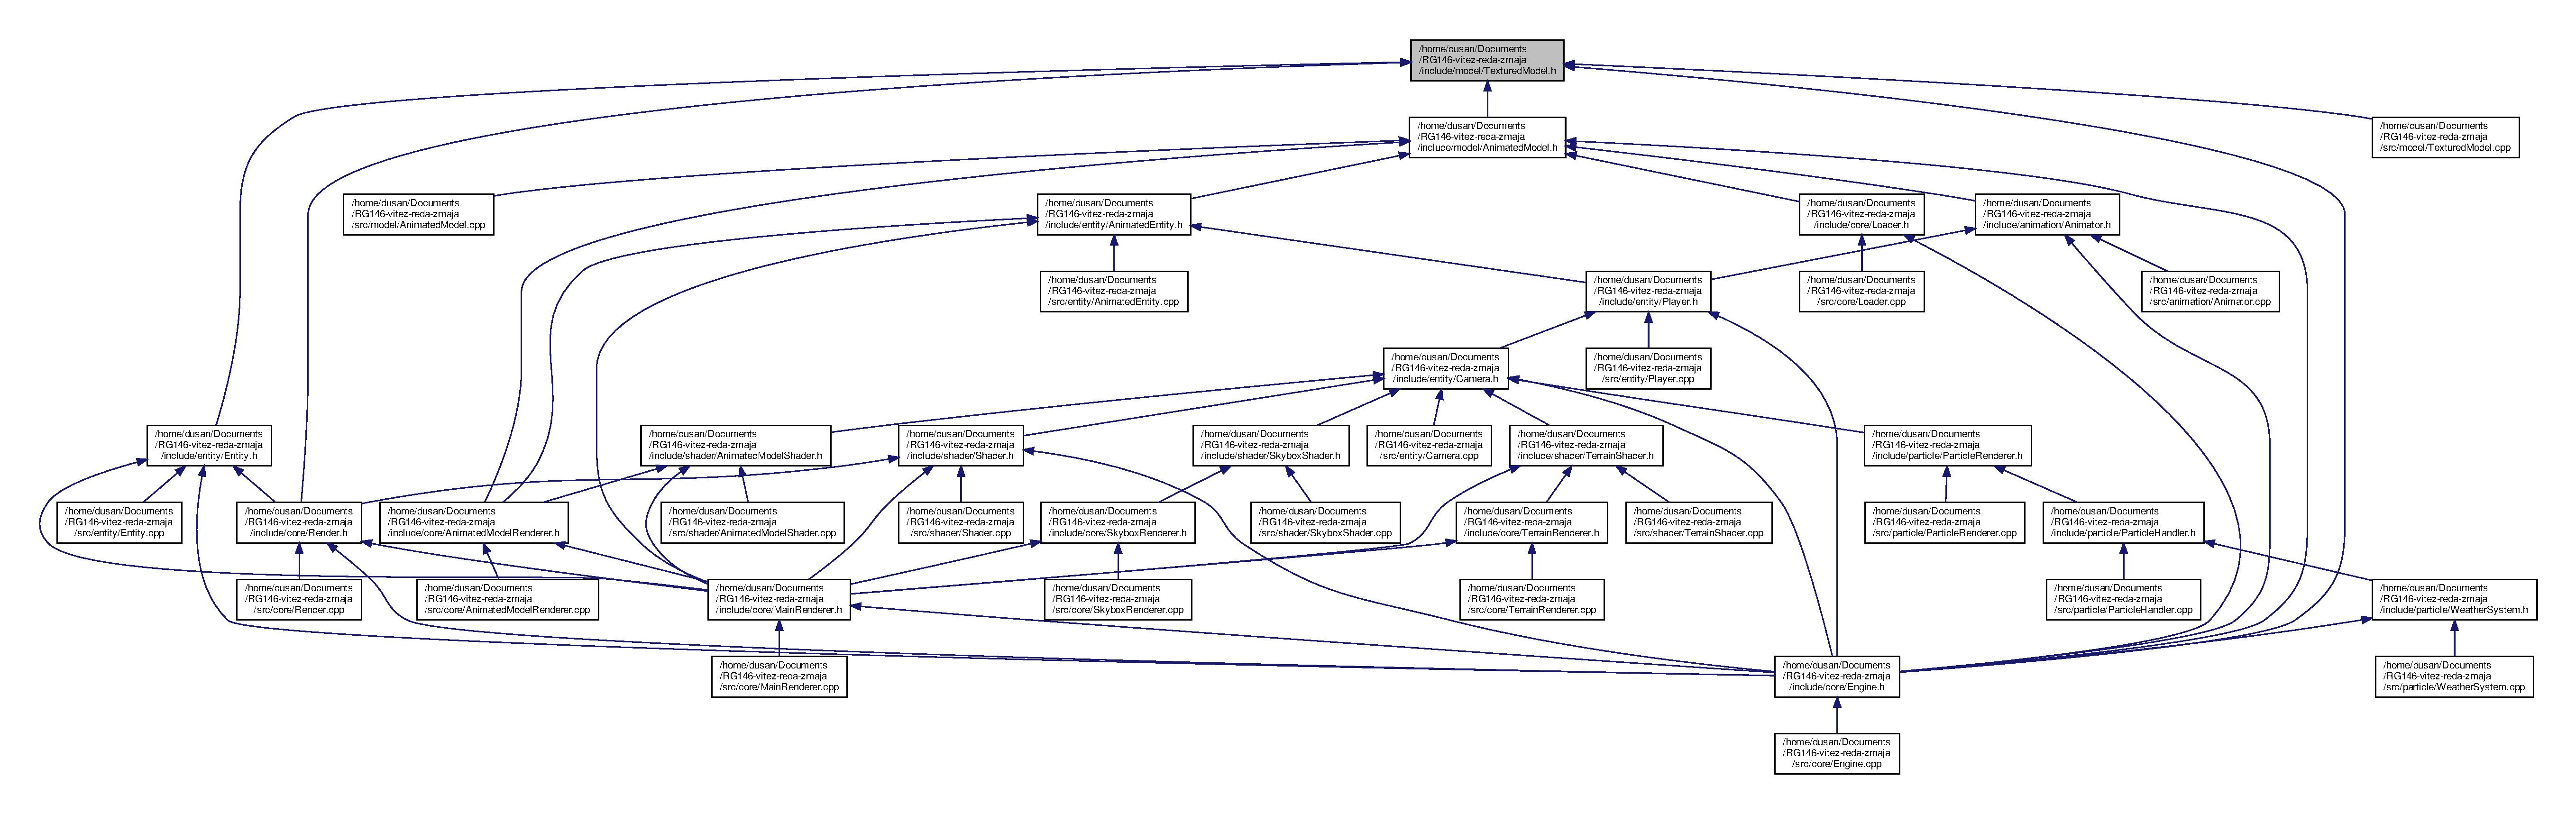
\includegraphics[width=350pt]{TexturedModel_8h__dep__incl}
\end{center}
\end{figure}
\subsection*{Klase, strukture i unije}
\begin{DoxyCompactItemize}
\item 
class \hyperlink{classmodel_1_1TexturedModel}{model\+::\+Textured\+Model}
\begin{DoxyCompactList}\small\item\em Klasa \hyperlink{classmodel_1_1TexturedModel}{Textured\+Model} opisuje model objekta zajedno sa teksturom. Model je opisan instancom klase \hyperlink{classmodel_1_1RawModel}{Raw\+Model} i odgovarajucom teksturom objekta pomocu instance klase Texture. \end{DoxyCompactList}\end{DoxyCompactItemize}
\subsection*{Prostori imena}
\begin{DoxyCompactItemize}
\item 
 \hyperlink{namespacemodel}{model}
\begin{DoxyCompactList}\small\item\em Prostor imena model. Sadrzi sve klase, funkcije i promenljive koje opisuju model objekta. \end{DoxyCompactList}\end{DoxyCompactItemize}


\subsection{Opširniji opis}
Deklaracija klase Textured\+Model. 

\begin{DoxyAuthor}{Autor}
Dusan Pantelic 
\end{DoxyAuthor}
\begin{DoxyDate}{Datum}
Januar 2017 
\end{DoxyDate}

\hypertarget{Shader_8h}{}\section{Opis datoteke /home/dusan/\+Documents/\+R\+G146-\/vitez-\/reda-\/zmaja/include/shader/\+Shader.h}
\label{Shader_8h}\index{/home/dusan/\+Documents/\+R\+G146-\/vitez-\/reda-\/zmaja/include/shader/\+Shader.\+h@{/home/dusan/\+Documents/\+R\+G146-\/vitez-\/reda-\/zmaja/include/shader/\+Shader.\+h}}


Deklaracija klase Shader.  


{\ttfamily \#include \char`\"{}../utility/\+Math.\+h\char`\"{}}\newline
{\ttfamily \#include \char`\"{}../entity/\+Camera.\+h\char`\"{}}\newline
{\ttfamily \#include \char`\"{}../entity/\+Light.\+h\char`\"{}}\newline
{\ttfamily \#include $<$G\+L/glut.\+h$>$}\newline
{\ttfamily \#include $<$iostream$>$}\newline
{\ttfamily \#include $<$vector$>$}\newline
{\ttfamily \#include $<$fstream$>$}\newline
{\ttfamily \#include $<$string$>$}\newline
{\ttfamily \#include $<$glm/vec3.\+hpp$>$}\newline
{\ttfamily \#include $<$glm/mat4x4.\+hpp$>$}\newline
{\ttfamily \#include $<$glm/gtc/matrix\+\_\+transform.\+hpp$>$}\newline
{\ttfamily \#include $<$glm/gtc/type\+\_\+ptr.\+hpp$>$}\newline
Graf zavisnosti datoteka za Shader.\+h\+:\nopagebreak
\begin{figure}[H]
\begin{center}
\leavevmode
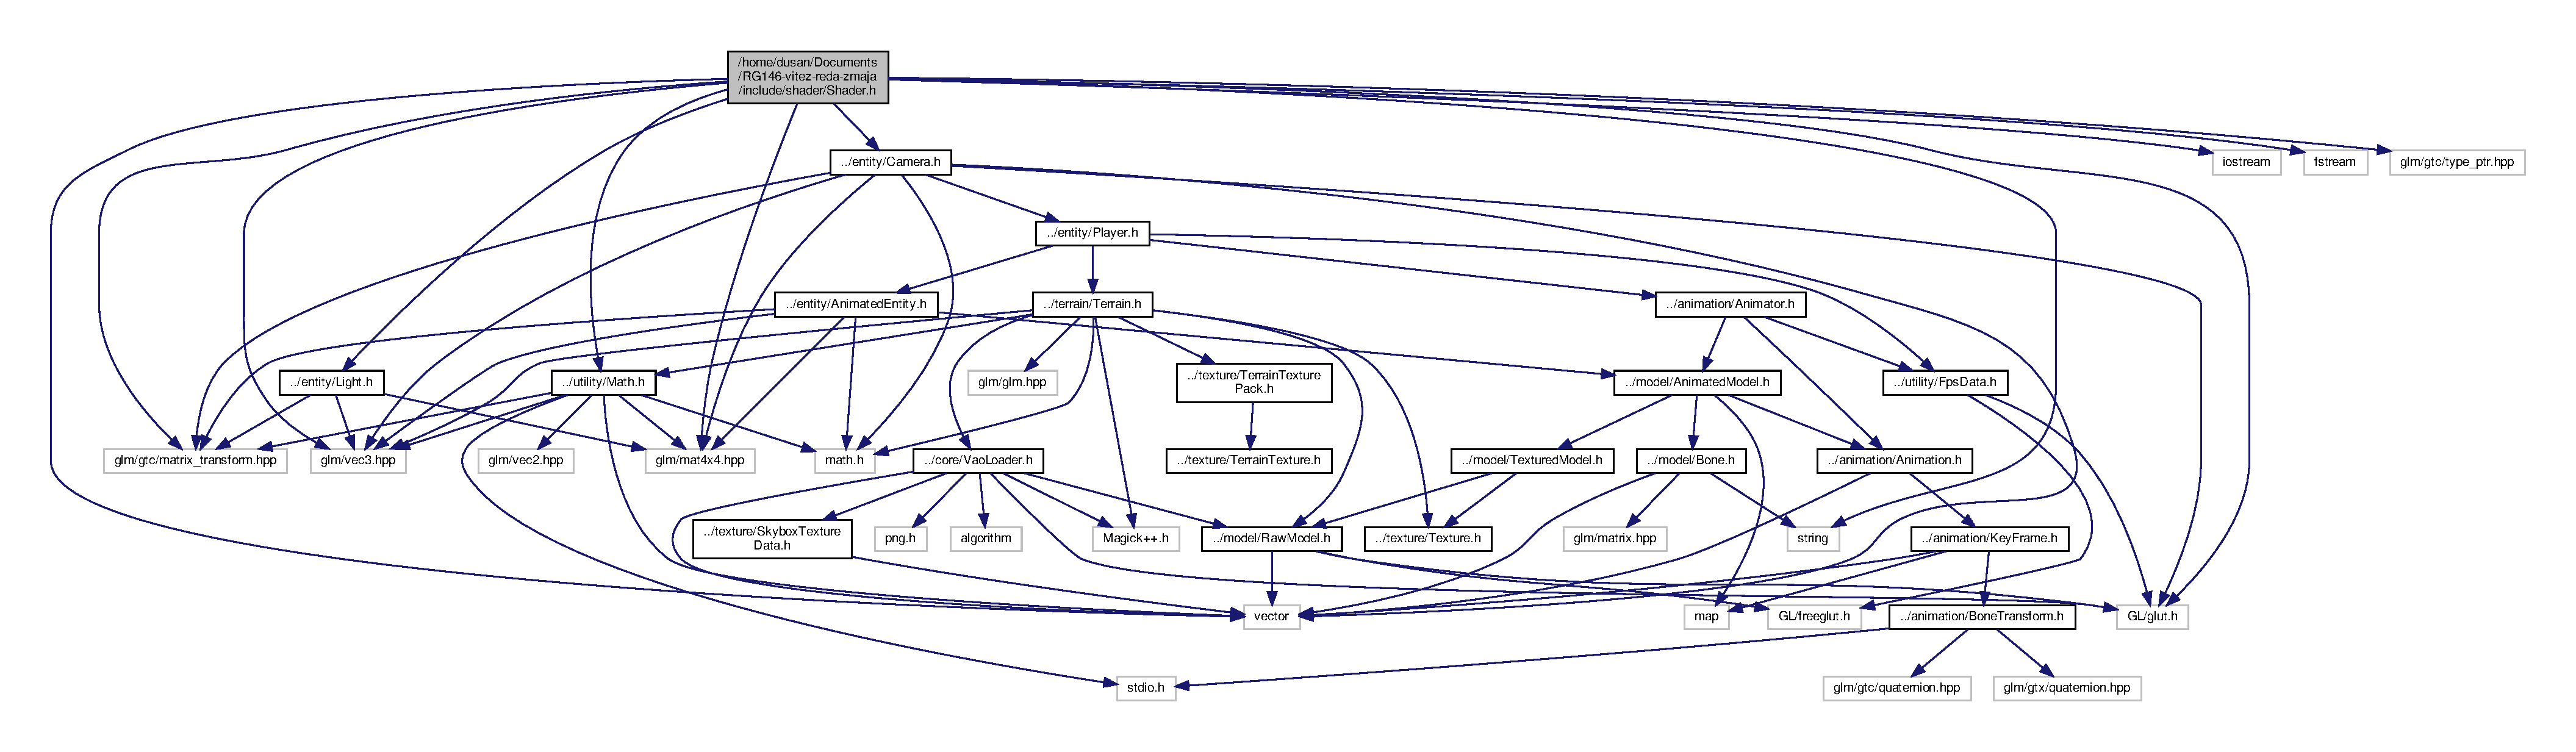
\includegraphics[width=350pt]{Shader_8h__incl}
\end{center}
\end{figure}
Ovaj graf pokazuje koje datoteke direktno ili indirektno uključuju ovu datoteku\+: \nopagebreak
\begin{figure}[H]
\begin{center}
\leavevmode
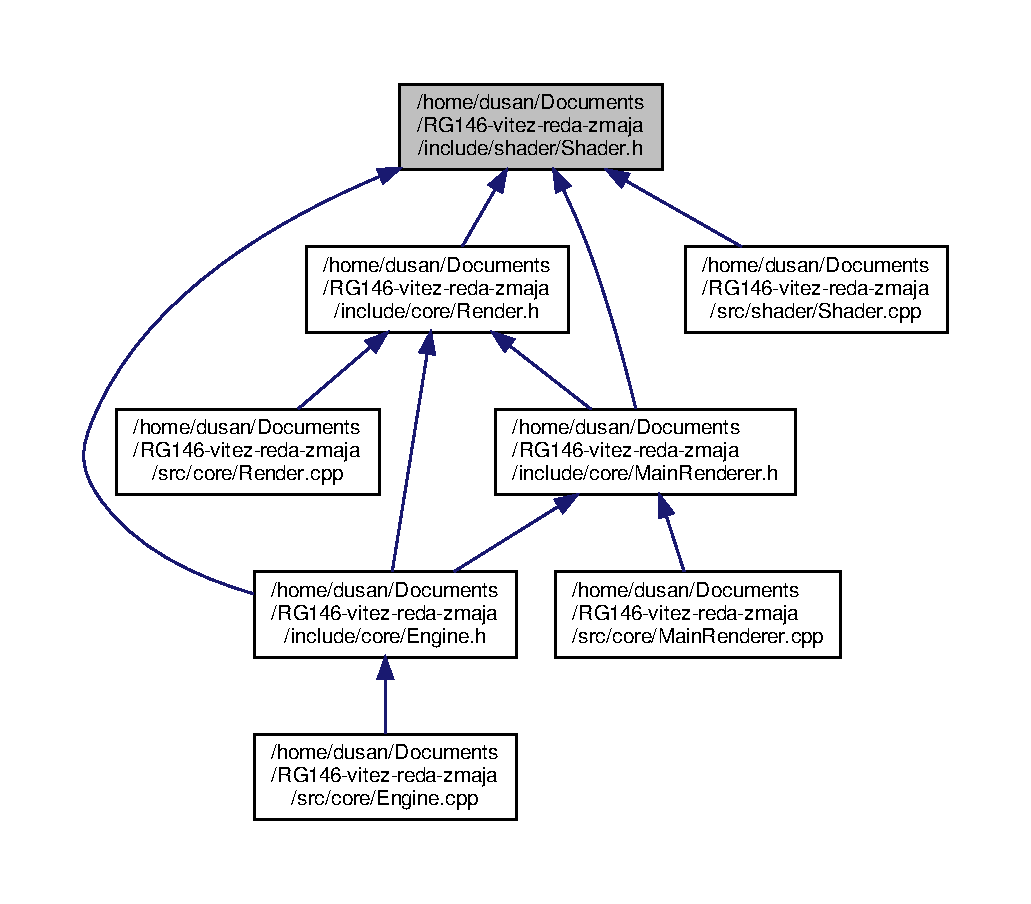
\includegraphics[width=350pt]{Shader_8h__dep__incl}
\end{center}
\end{figure}
\subsection*{Klase, strukture i unije}
\begin{DoxyCompactItemize}
\item 
class \hyperlink{classshader_1_1Shader}{shader\+::\+Shader}
\begin{DoxyCompactList}\small\item\em Klasa \hyperlink{classshader_1_1Shader}{Shader} ucitava i izvrsava programe na Open\+GL Shading jeziku. Ucitavaju se sejder fajlovi koji se zatim kompajliraju i po potrebi se izvrsavaju i zaustavljaju. \end{DoxyCompactList}\end{DoxyCompactItemize}
\subsection*{Prostori imena}
\begin{DoxyCompactItemize}
\item 
 \hyperlink{namespaceshader}{shader}
\begin{DoxyCompactList}\small\item\em Prostor imena shader. Sadrzi sejder programe. \end{DoxyCompactList}\end{DoxyCompactItemize}
\subsection*{Makro zamene}
\begin{DoxyCompactItemize}
\item 
\#define \hyperlink{Shader_8h_a120fb070bddb21f0bd899f50252c4cb5}{G\+L\+\_\+\+G\+L\+E\+X\+T\+\_\+\+P\+R\+O\+T\+O\+T\+Y\+P\+ES}
\end{DoxyCompactItemize}


\subsection{Opširniji opis}
Deklaracija klase Shader. 

\begin{DoxyAuthor}{Autor}
Dusan Pantelic 
\end{DoxyAuthor}
\begin{DoxyDate}{Datum}
Januar 2017 
\end{DoxyDate}


\subsection{Dokumentacija makro zamene}
\mbox{\Hypertarget{Shader_8h_a120fb070bddb21f0bd899f50252c4cb5}\label{Shader_8h_a120fb070bddb21f0bd899f50252c4cb5}} 
\index{Shader.\+h@{Shader.\+h}!G\+L\+\_\+\+G\+L\+E\+X\+T\+\_\+\+P\+R\+O\+T\+O\+T\+Y\+P\+ES@{G\+L\+\_\+\+G\+L\+E\+X\+T\+\_\+\+P\+R\+O\+T\+O\+T\+Y\+P\+ES}}
\index{G\+L\+\_\+\+G\+L\+E\+X\+T\+\_\+\+P\+R\+O\+T\+O\+T\+Y\+P\+ES@{G\+L\+\_\+\+G\+L\+E\+X\+T\+\_\+\+P\+R\+O\+T\+O\+T\+Y\+P\+ES}!Shader.\+h@{Shader.\+h}}
\subsubsection{\texorpdfstring{G\+L\+\_\+\+G\+L\+E\+X\+T\+\_\+\+P\+R\+O\+T\+O\+T\+Y\+P\+ES}{GL\_GLEXT\_PROTOTYPES}}
{\footnotesize\ttfamily \#define G\+L\+\_\+\+G\+L\+E\+X\+T\+\_\+\+P\+R\+O\+T\+O\+T\+Y\+P\+ES}


\hypertarget{TerrainShader_8h}{}\section{Opis datoteke /home/dusan/\+Documents/\+R\+G146-\/vitez-\/reda-\/zmaja/include/shader/\+Terrain\+Shader.h}
\label{TerrainShader_8h}\index{/home/dusan/\+Documents/\+R\+G146-\/vitez-\/reda-\/zmaja/include/shader/\+Terrain\+Shader.\+h@{/home/dusan/\+Documents/\+R\+G146-\/vitez-\/reda-\/zmaja/include/shader/\+Terrain\+Shader.\+h}}


Deklaracija klase Terrain\+Shader.  


{\ttfamily \#include \char`\"{}../utility/\+Math.\+h\char`\"{}}\newline
{\ttfamily \#include \char`\"{}../entity/\+Camera.\+h\char`\"{}}\newline
{\ttfamily \#include \char`\"{}../entity/\+Light.\+h\char`\"{}}\newline
{\ttfamily \#include $<$G\+L/glut.\+h$>$}\newline
{\ttfamily \#include $<$iostream$>$}\newline
{\ttfamily \#include $<$vector$>$}\newline
{\ttfamily \#include $<$fstream$>$}\newline
{\ttfamily \#include $<$string$>$}\newline
{\ttfamily \#include $<$glm/vec3.\+hpp$>$}\newline
{\ttfamily \#include $<$glm/mat4x4.\+hpp$>$}\newline
{\ttfamily \#include $<$glm/gtc/matrix\+\_\+transform.\+hpp$>$}\newline
{\ttfamily \#include $<$glm/gtc/type\+\_\+ptr.\+hpp$>$}\newline
Graf zavisnosti datoteka za Terrain\+Shader.\+h\+:
\nopagebreak
\begin{figure}[H]
\begin{center}
\leavevmode
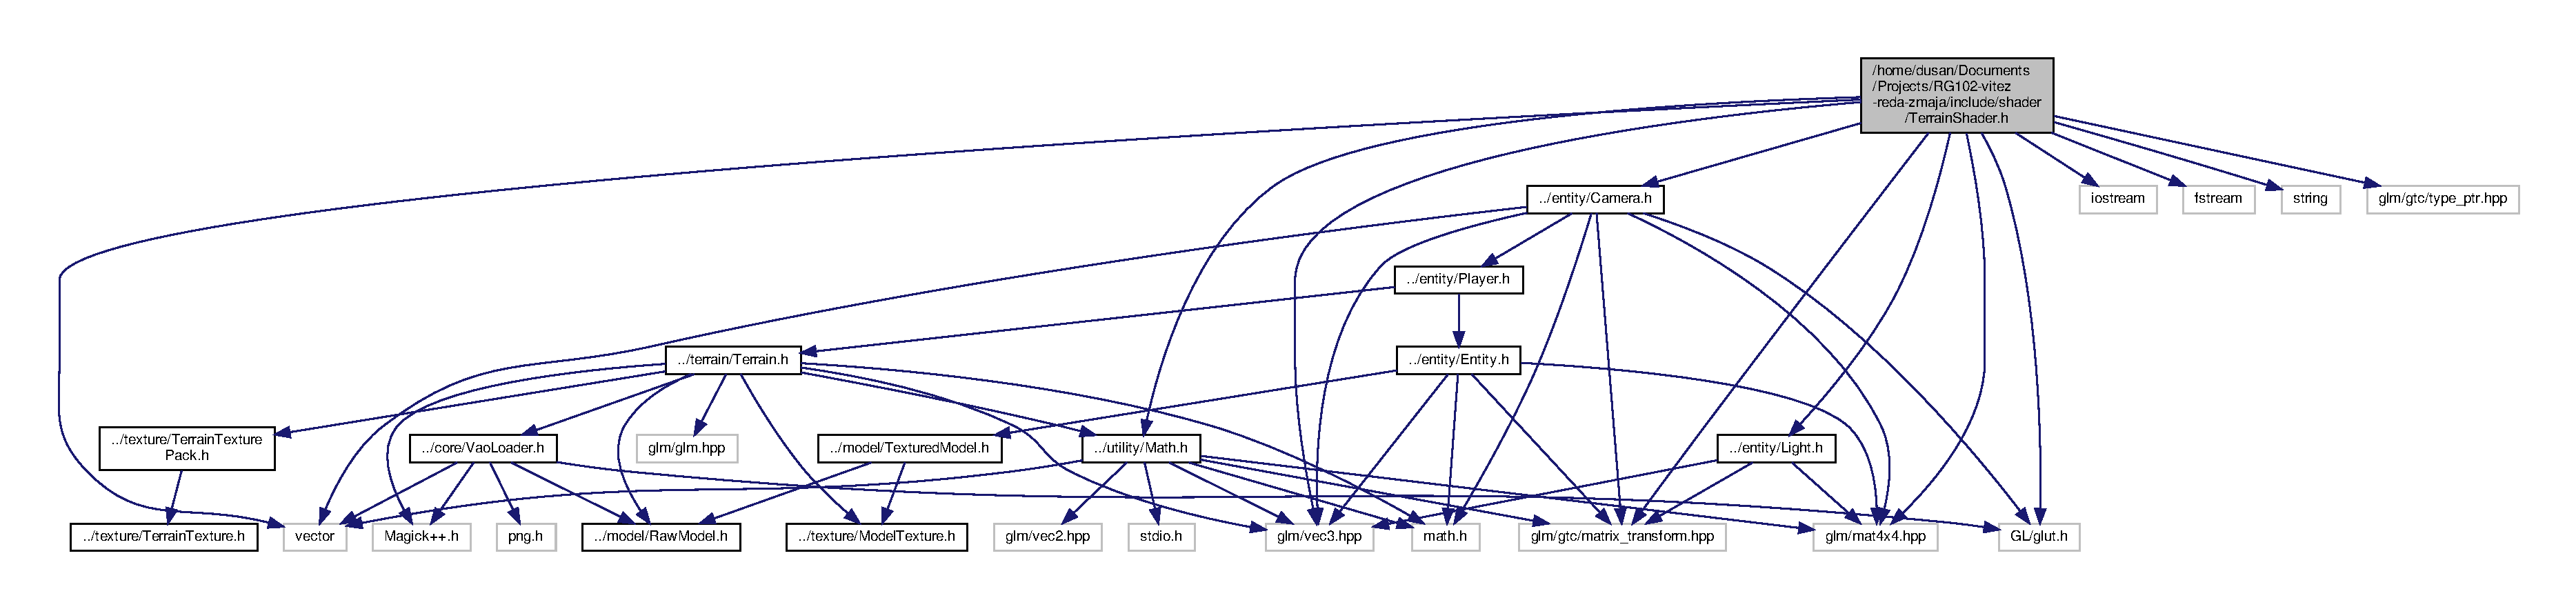
\includegraphics[width=350pt]{TerrainShader_8h__incl}
\end{center}
\end{figure}
Ovaj graf pokazuje koje datoteke direktno ili indirektno uključuju ovu datoteku\+: 
\nopagebreak
\begin{figure}[H]
\begin{center}
\leavevmode
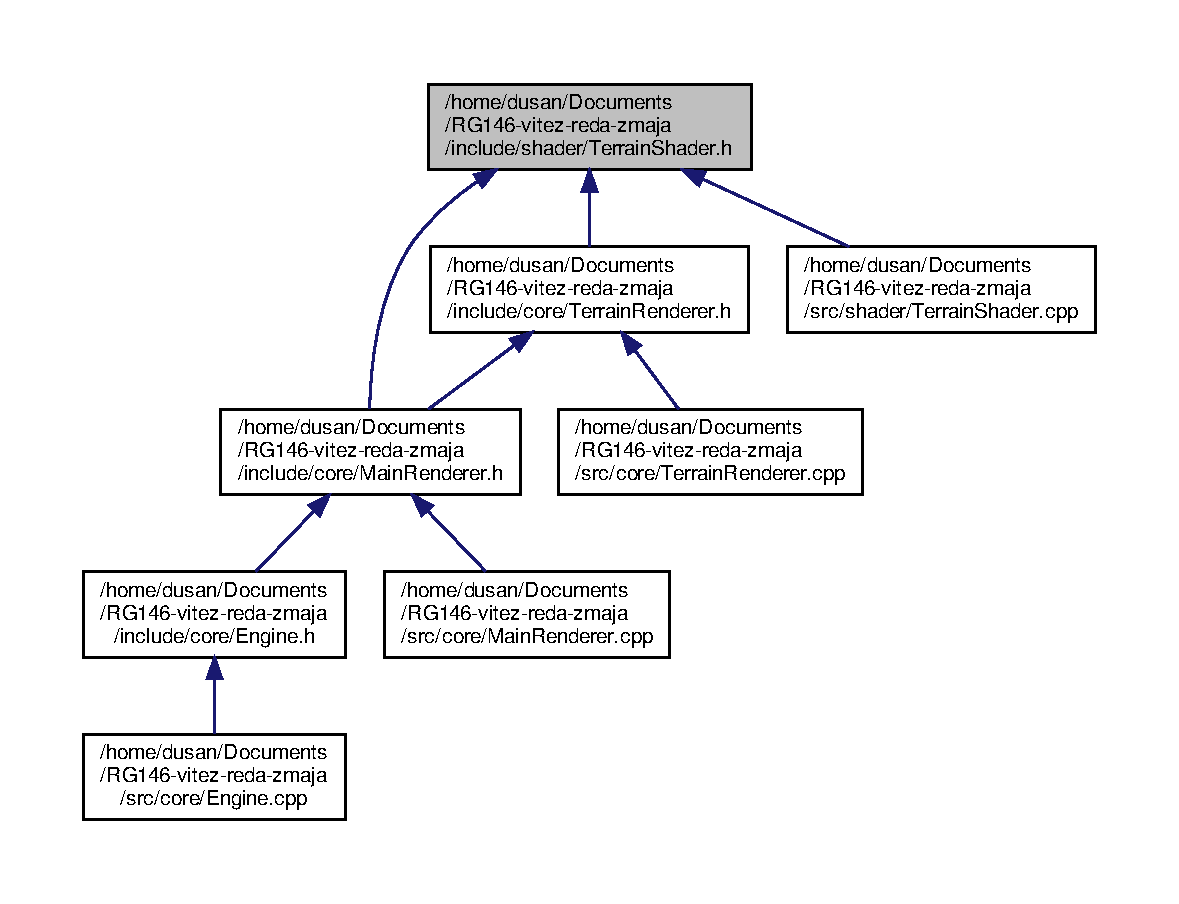
\includegraphics[width=350pt]{TerrainShader_8h__dep__incl}
\end{center}
\end{figure}
\subsection*{Klase, strukture i unije}
\begin{DoxyCompactItemize}
\item 
class \hyperlink{classshader_1_1TerrainShader}{shader\+::\+Terrain\+Shader}
\begin{DoxyCompactList}\small\item\em Klasa \hyperlink{classshader_1_1TerrainShader}{Terrain\+Shader} ucitava i izvrsava programe na Open\+GL Shading jeziku. Ucitavaju se sejder fajlovi koji se zatim kompajliraju i po potrebi se izvrsavaju i zaustavljaju. \end{DoxyCompactList}\end{DoxyCompactItemize}
\subsection*{Prostori imena}
\begin{DoxyCompactItemize}
\item 
 \hyperlink{namespaceshader}{shader}
\begin{DoxyCompactList}\small\item\em Prostor imena shader. Sadrzi sejder programe. \end{DoxyCompactList}\end{DoxyCompactItemize}
\subsection*{Makro zamene}
\begin{DoxyCompactItemize}
\item 
\#define \hyperlink{TerrainShader_8h_a120fb070bddb21f0bd899f50252c4cb5}{G\+L\+\_\+\+G\+L\+E\+X\+T\+\_\+\+P\+R\+O\+T\+O\+T\+Y\+P\+ES}
\end{DoxyCompactItemize}


\subsection{Opširniji opis}
Deklaracija klase Terrain\+Shader. 

\begin{DoxyAuthor}{Autor}
Dusan Pantelic 
\end{DoxyAuthor}
\begin{DoxyDate}{Datum}
Januar 2017 
\end{DoxyDate}


\subsection{Dokumentacija makro zamene}
\mbox{\Hypertarget{TerrainShader_8h_a120fb070bddb21f0bd899f50252c4cb5}\label{TerrainShader_8h_a120fb070bddb21f0bd899f50252c4cb5}} 
\index{Terrain\+Shader.\+h@{Terrain\+Shader.\+h}!G\+L\+\_\+\+G\+L\+E\+X\+T\+\_\+\+P\+R\+O\+T\+O\+T\+Y\+P\+ES@{G\+L\+\_\+\+G\+L\+E\+X\+T\+\_\+\+P\+R\+O\+T\+O\+T\+Y\+P\+ES}}
\index{G\+L\+\_\+\+G\+L\+E\+X\+T\+\_\+\+P\+R\+O\+T\+O\+T\+Y\+P\+ES@{G\+L\+\_\+\+G\+L\+E\+X\+T\+\_\+\+P\+R\+O\+T\+O\+T\+Y\+P\+ES}!Terrain\+Shader.\+h@{Terrain\+Shader.\+h}}
\subsubsection{\texorpdfstring{G\+L\+\_\+\+G\+L\+E\+X\+T\+\_\+\+P\+R\+O\+T\+O\+T\+Y\+P\+ES}{GL\_GLEXT\_PROTOTYPES}}
{\footnotesize\ttfamily \#define G\+L\+\_\+\+G\+L\+E\+X\+T\+\_\+\+P\+R\+O\+T\+O\+T\+Y\+P\+ES}


\hypertarget{Terrain_8h}{}\section{Opis datoteke /home/dusan/\+Documents/\+R\+G146-\/vitez-\/reda-\/zmaja/include/terrain/\+Terrain.h}
\label{Terrain_8h}\index{/home/dusan/\+Documents/\+R\+G146-\/vitez-\/reda-\/zmaja/include/terrain/\+Terrain.\+h@{/home/dusan/\+Documents/\+R\+G146-\/vitez-\/reda-\/zmaja/include/terrain/\+Terrain.\+h}}


Deklaracija klase Terrain.  


{\ttfamily \#include \char`\"{}../model/\+Raw\+Model.\+h\char`\"{}}\newline
{\ttfamily \#include \char`\"{}../texture/\+Texture.\+h\char`\"{}}\newline
{\ttfamily \#include \char`\"{}../texture/\+Terrain\+Texture\+Pack.\+h\char`\"{}}\newline
{\ttfamily \#include \char`\"{}../core/\+Vao\+Loader.\+h\char`\"{}}\newline
{\ttfamily \#include \char`\"{}../utility/\+Math.\+h\char`\"{}}\newline
{\ttfamily \#include $<$Magick++.\+h$>$}\newline
{\ttfamily \#include $<$math.\+h$>$}\newline
{\ttfamily \#include $<$glm/vec3.\+hpp$>$}\newline
{\ttfamily \#include $<$glm/glm.\+hpp$>$}\newline
Graf zavisnosti datoteka za Terrain.\+h\+:
\nopagebreak
\begin{figure}[H]
\begin{center}
\leavevmode
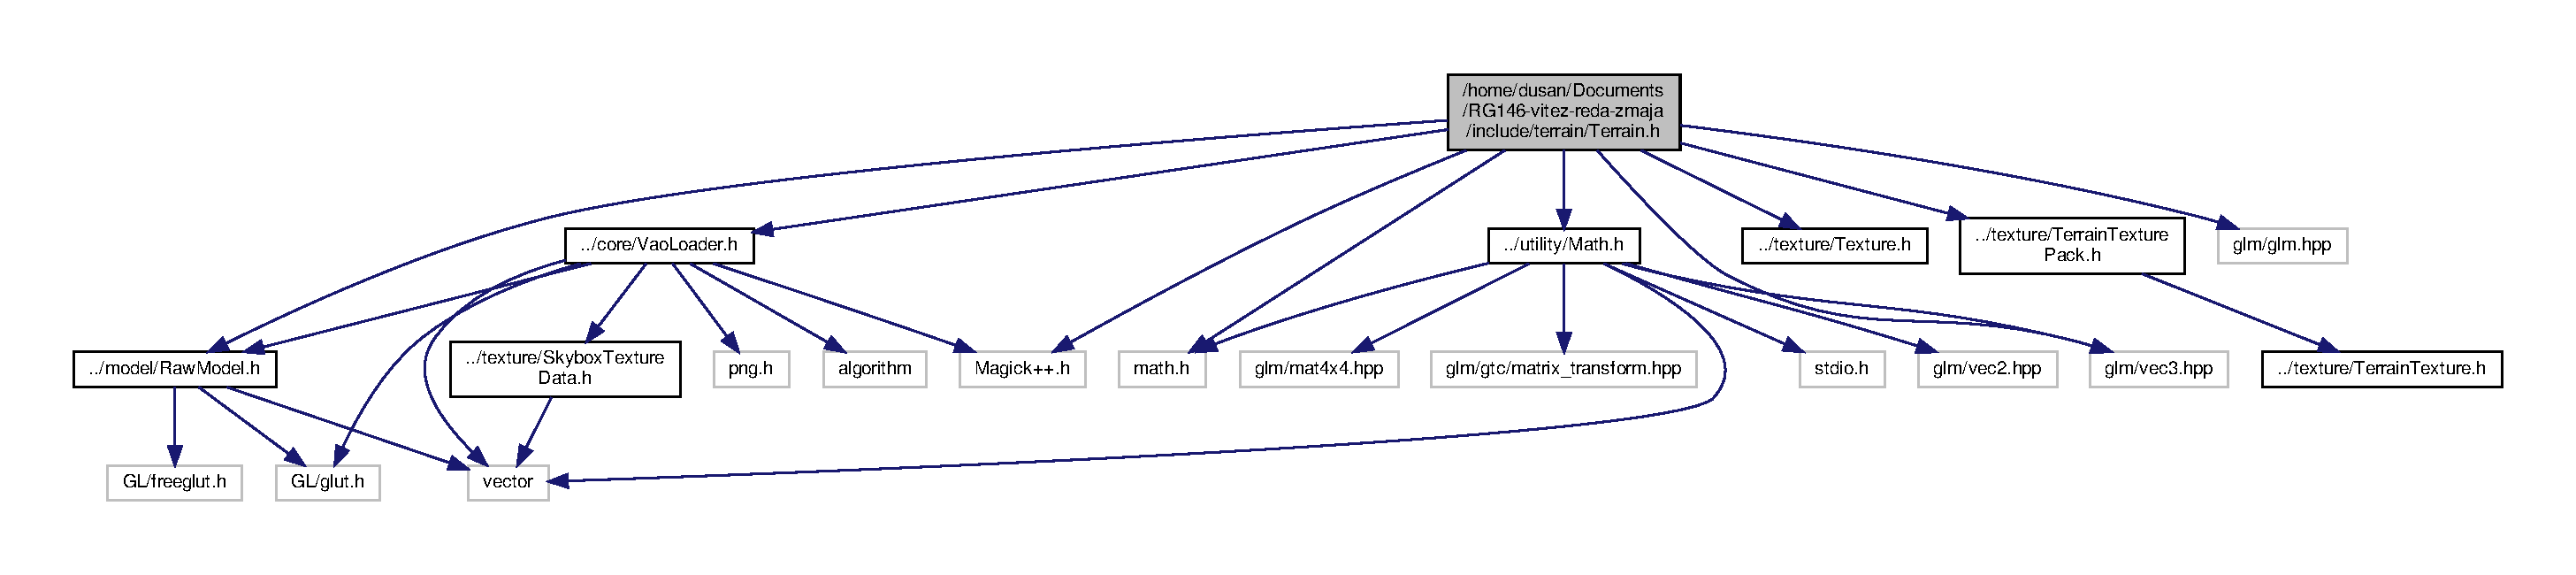
\includegraphics[width=350pt]{Terrain_8h__incl}
\end{center}
\end{figure}
Ovaj graf pokazuje koje datoteke direktno ili indirektno uključuju ovu datoteku\+: 
\nopagebreak
\begin{figure}[H]
\begin{center}
\leavevmode
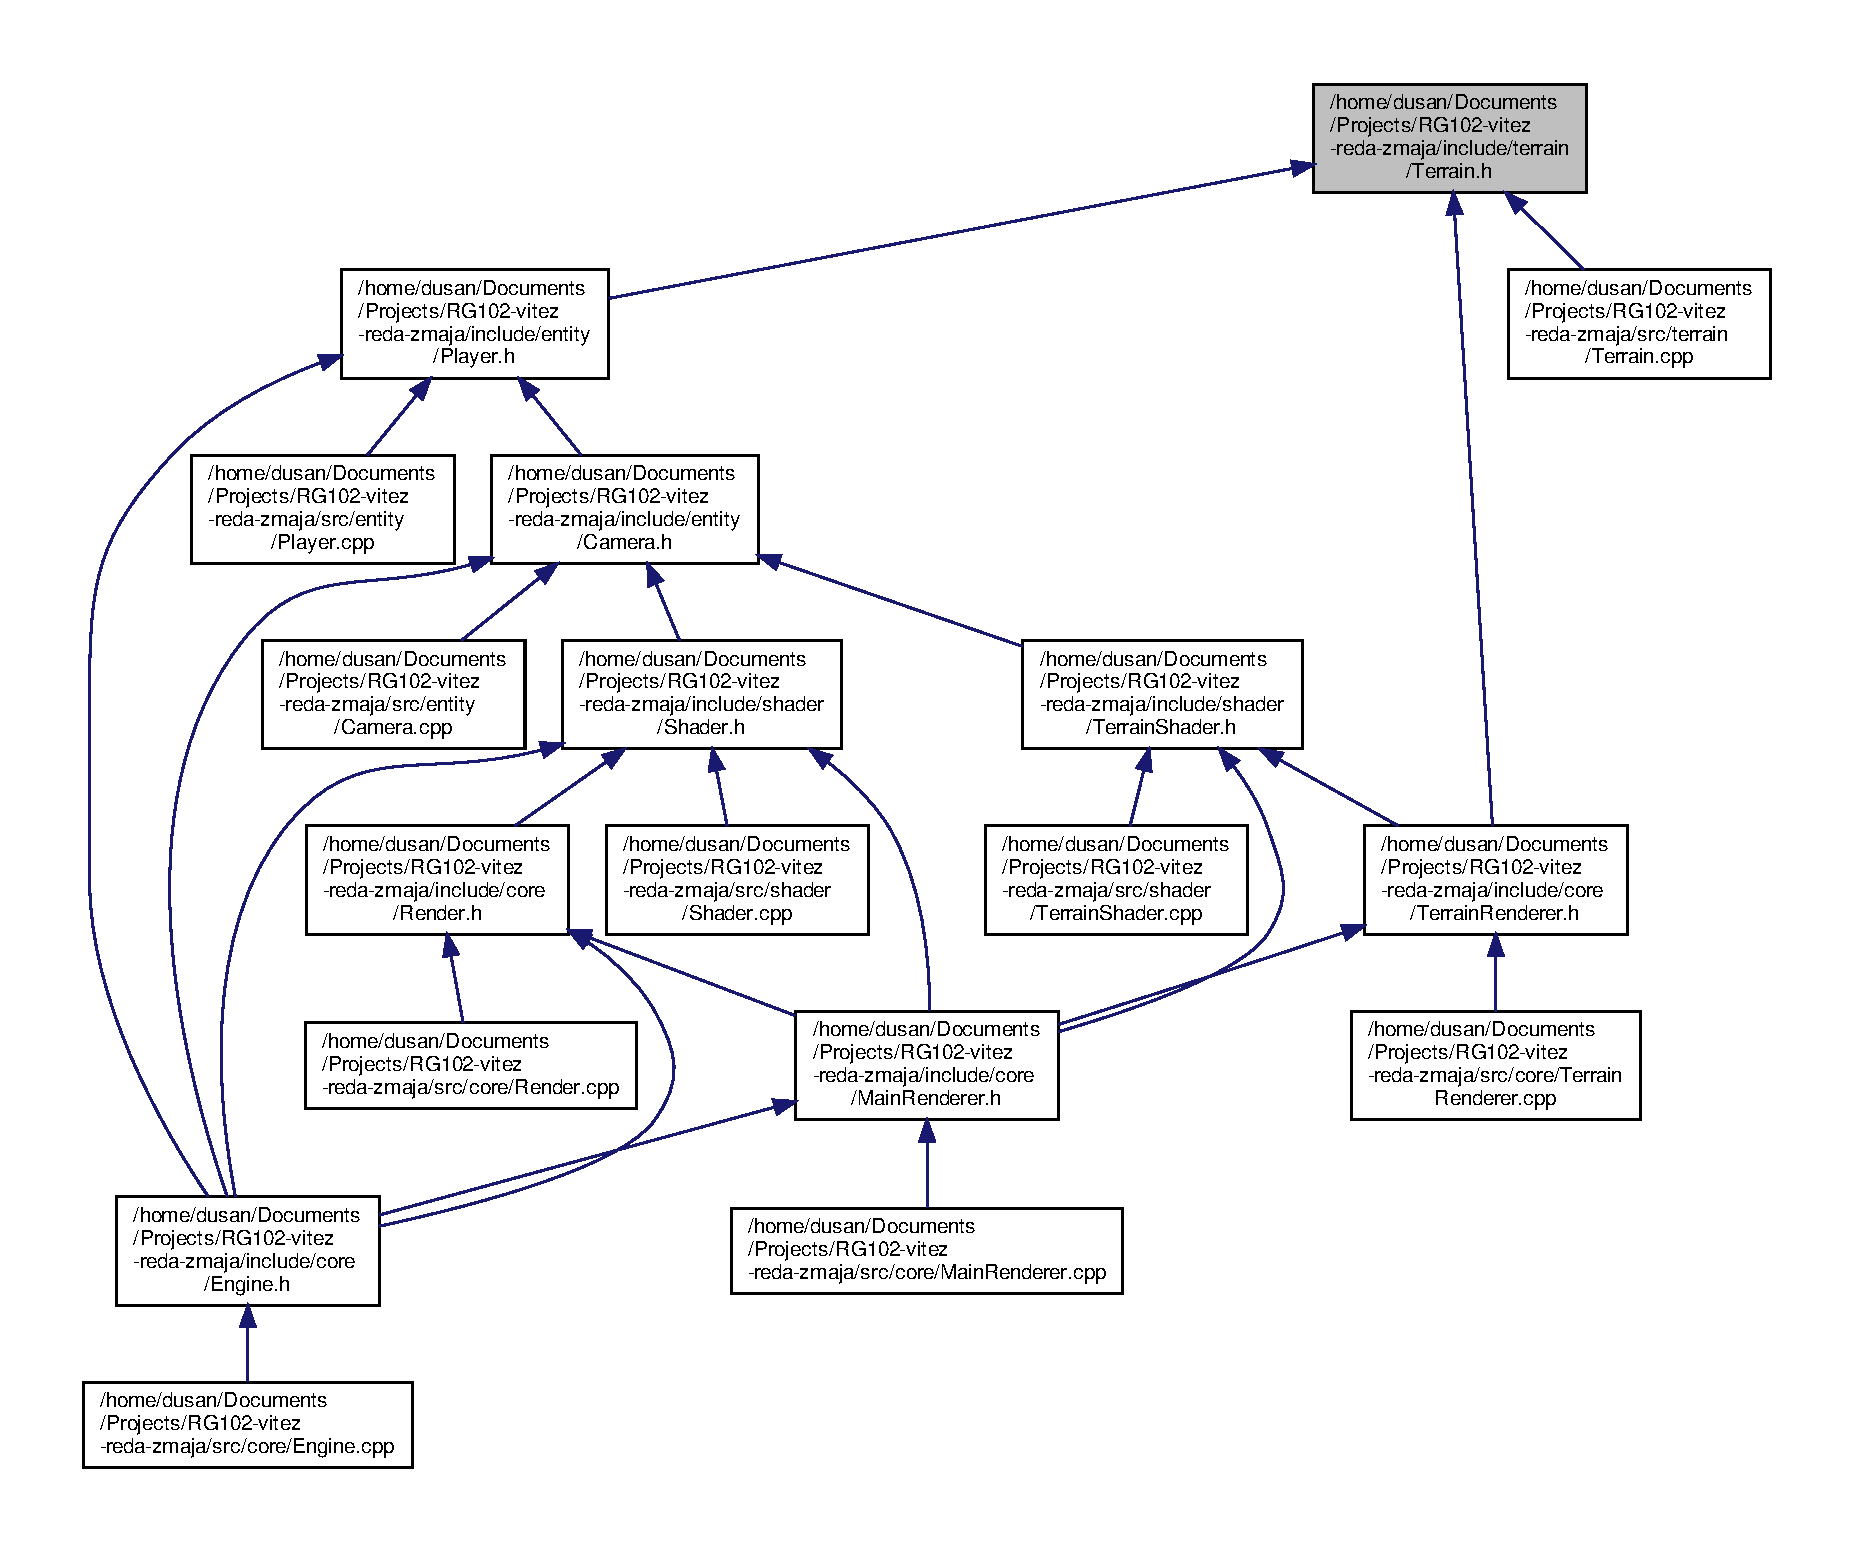
\includegraphics[width=350pt]{Terrain_8h__dep__incl}
\end{center}
\end{figure}
\subsection*{Klase, strukture i unije}
\begin{DoxyCompactItemize}
\item 
class \hyperlink{classterrain_1_1Terrain}{terrain\+::\+Terrain}
\begin{DoxyCompactList}\small\item\em Klasa \hyperlink{classterrain_1_1Terrain}{Terrain} zaduzena je za kreiranje terena. Pomocu klase \hyperlink{classterrain_1_1Terrain}{Terrain} generisemo teren na osnovu visinske mape. \end{DoxyCompactList}\end{DoxyCompactItemize}
\subsection*{Prostori imena}
\begin{DoxyCompactItemize}
\item 
 \hyperlink{namespaceterrain}{terrain}
\begin{DoxyCompactList}\small\item\em Prostor imena terain. Sadrzi sve klase, funkcije i promenljive za kreiranje i rad sa terenom. \end{DoxyCompactList}\end{DoxyCompactItemize}
\subsection*{Makro zamene}
\begin{DoxyCompactItemize}
\item 
\#define \hyperlink{Terrain_8h_a70ed59adcb4159ac551058053e649640}{S\+I\+ZE}~1000
\item 
\#define \hyperlink{Terrain_8h_ac1689bb03dbfff43e32aff331b96dea8}{M\+A\+X\+\_\+\+P\+I\+X\+E\+L\+\_\+\+C\+O\+L\+O\+UR}~256$\ast$256$\ast$256
\item 
\#define \hyperlink{Terrain_8h_a9059fa76eb5e8e86f870405d63e72c4c}{M\+A\+X\+\_\+\+H\+E\+I\+G\+HT}~60
\end{DoxyCompactItemize}


\subsection{Opširniji opis}
Deklaracija klase Terrain. 

\begin{DoxyAuthor}{Autor}
Dusan Pantelic 
\end{DoxyAuthor}
\begin{DoxyDate}{Datum}
Septembar 2018 
\end{DoxyDate}


\subsection{Dokumentacija makro zamene}
\mbox{\Hypertarget{Terrain_8h_a9059fa76eb5e8e86f870405d63e72c4c}\label{Terrain_8h_a9059fa76eb5e8e86f870405d63e72c4c}} 
\index{Terrain.\+h@{Terrain.\+h}!M\+A\+X\+\_\+\+H\+E\+I\+G\+HT@{M\+A\+X\+\_\+\+H\+E\+I\+G\+HT}}
\index{M\+A\+X\+\_\+\+H\+E\+I\+G\+HT@{M\+A\+X\+\_\+\+H\+E\+I\+G\+HT}!Terrain.\+h@{Terrain.\+h}}
\subsubsection{\texorpdfstring{M\+A\+X\+\_\+\+H\+E\+I\+G\+HT}{MAX\_HEIGHT}}
{\footnotesize\ttfamily \#define M\+A\+X\+\_\+\+H\+E\+I\+G\+HT~60}

\mbox{\Hypertarget{Terrain_8h_ac1689bb03dbfff43e32aff331b96dea8}\label{Terrain_8h_ac1689bb03dbfff43e32aff331b96dea8}} 
\index{Terrain.\+h@{Terrain.\+h}!M\+A\+X\+\_\+\+P\+I\+X\+E\+L\+\_\+\+C\+O\+L\+O\+UR@{M\+A\+X\+\_\+\+P\+I\+X\+E\+L\+\_\+\+C\+O\+L\+O\+UR}}
\index{M\+A\+X\+\_\+\+P\+I\+X\+E\+L\+\_\+\+C\+O\+L\+O\+UR@{M\+A\+X\+\_\+\+P\+I\+X\+E\+L\+\_\+\+C\+O\+L\+O\+UR}!Terrain.\+h@{Terrain.\+h}}
\subsubsection{\texorpdfstring{M\+A\+X\+\_\+\+P\+I\+X\+E\+L\+\_\+\+C\+O\+L\+O\+UR}{MAX\_PIXEL\_COLOUR}}
{\footnotesize\ttfamily \#define M\+A\+X\+\_\+\+P\+I\+X\+E\+L\+\_\+\+C\+O\+L\+O\+UR~256$\ast$256$\ast$256}

\mbox{\Hypertarget{Terrain_8h_a70ed59adcb4159ac551058053e649640}\label{Terrain_8h_a70ed59adcb4159ac551058053e649640}} 
\index{Terrain.\+h@{Terrain.\+h}!S\+I\+ZE@{S\+I\+ZE}}
\index{S\+I\+ZE@{S\+I\+ZE}!Terrain.\+h@{Terrain.\+h}}
\subsubsection{\texorpdfstring{S\+I\+ZE}{SIZE}}
{\footnotesize\ttfamily \#define S\+I\+ZE~1000}


\hypertarget{Texture_8h}{}\section{Opis datoteke /home/dusan/\+Documents/\+R\+G146-\/vitez-\/reda-\/zmaja/include/texture/\+Model\+Texture.h}
\label{Texture_8h}\index{/home/dusan/\+Documents/\+R\+G146-\/vitez-\/reda-\/zmaja/include/texture/\+Model\+Texture.\+h@{/home/dusan/\+Documents/\+R\+G146-\/vitez-\/reda-\/zmaja/include/texture/\+Model\+Texture.\+h}}


Deklaracija klase Model\+Texture.  


Ovaj graf pokazuje koje datoteke direktno ili indirektno uključuju ovu datoteku\+: \nopagebreak
\begin{figure}[H]
\begin{center}
\leavevmode
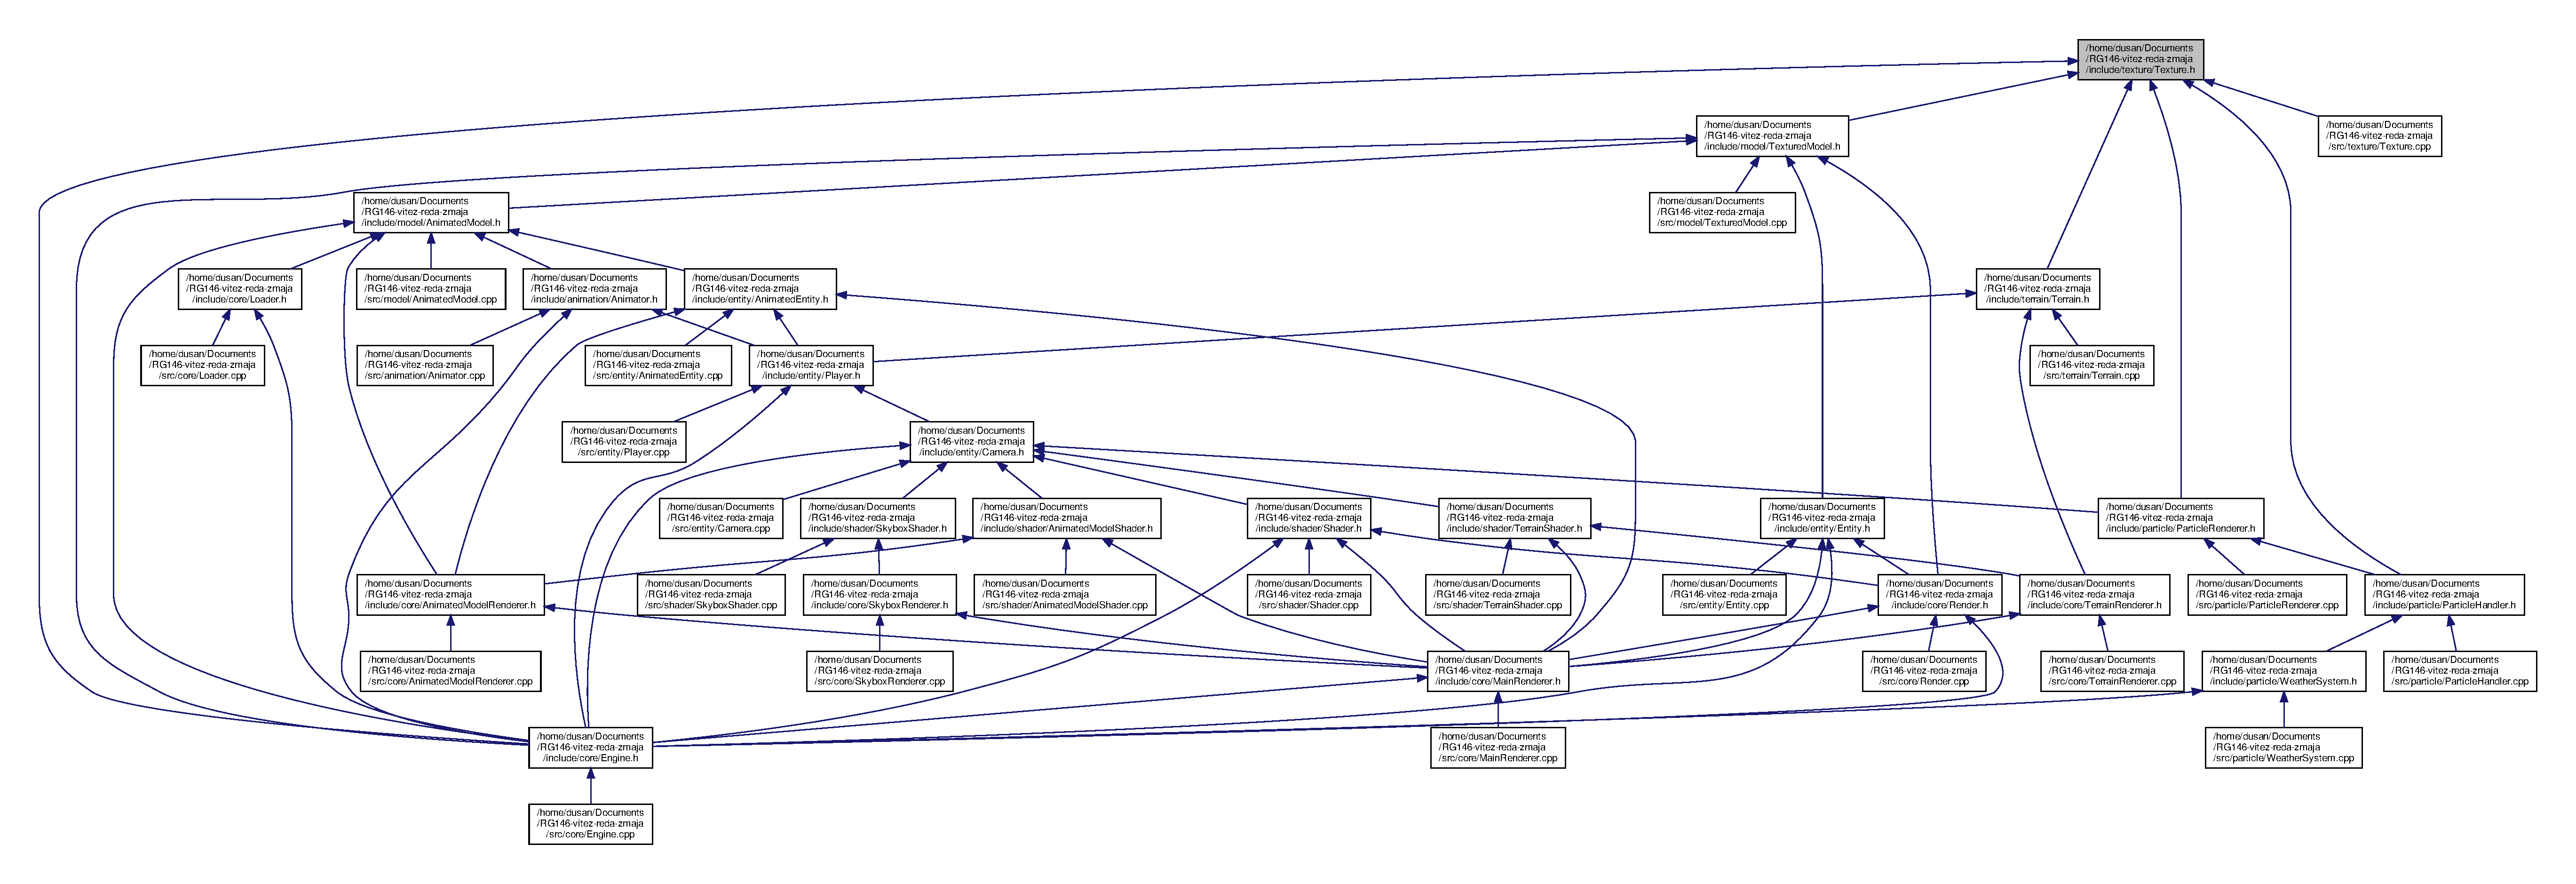
\includegraphics[width=350pt]{Texture_8h__dep__incl}
\end{center}
\end{figure}
\subsection*{Klase, strukture i unije}
\begin{DoxyCompactItemize}
\item 
class \hyperlink{classtexture_1_1Texture}{texture\+::\+Model\+Texture}
\begin{DoxyCompactList}\small\item\em Klasa Textured\+Model opisuje teksturu objekta. Model je opisan instancom klase Raw\+Model i odgovarajucom teksturom objekta pomocu instance klase \hyperlink{classtexture_1_1Texture}{Model\+Texture}. \end{DoxyCompactList}\end{DoxyCompactItemize}
\subsection*{Prostori imena}
\begin{DoxyCompactItemize}
\item 
 \hyperlink{namespacetexture}{texture}
\begin{DoxyCompactList}\small\item\em Prostor imena texture. Sadrzi sve klase, funkcije i promenljive koje opisuju teksturu objekta. \end{DoxyCompactList}\end{DoxyCompactItemize}


\subsection{Opširniji opis}
Deklaracija klase Model\+Texture. 

\begin{DoxyAuthor}{Autor}
Dusan Pantelic 
\end{DoxyAuthor}
\begin{DoxyDate}{Datum}
Januar 2017
\end{DoxyDate}
\begin{DoxyAuthor}{Autor}
Dusan Pantelic 
\end{DoxyAuthor}
\begin{DoxyDate}{Datum}
Avgust 2018 
\end{DoxyDate}

\hypertarget{TerrainTexture_8h}{}\section{Opis datoteke /home/dusan/\+Documents/\+R\+G146-\/vitez-\/reda-\/zmaja/include/texture/\+Terrain\+Texture.h}
\label{TerrainTexture_8h}\index{/home/dusan/\+Documents/\+R\+G146-\/vitez-\/reda-\/zmaja/include/texture/\+Terrain\+Texture.\+h@{/home/dusan/\+Documents/\+R\+G146-\/vitez-\/reda-\/zmaja/include/texture/\+Terrain\+Texture.\+h}}


Deklaracija klase Terrain\+Texture.  


Ovaj graf pokazuje koje datoteke direktno ili indirektno uključuju ovu datoteku\+: \nopagebreak
\begin{figure}[H]
\begin{center}
\leavevmode
\includegraphics[width=350pt]{TerrainTexture_8h__dep__incl}
\end{center}
\end{figure}
\subsection*{Klase, strukture i unije}
\begin{DoxyCompactItemize}
\item 
class \hyperlink{classtexture_1_1TerrainTexture}{texture\+::\+Terrain\+Texture}
\begin{DoxyCompactList}\small\item\em Klasa \hyperlink{classtexture_1_1TerrainTexture}{Terrain\+Texture} opisuje teksturu terena. \end{DoxyCompactList}\end{DoxyCompactItemize}
\subsection*{Prostori imena}
\begin{DoxyCompactItemize}
\item 
 \hyperlink{namespacetexture}{texture}
\begin{DoxyCompactList}\small\item\em Prostor imena texture. Sadrzi sve klase, funkcije i promenljive koje opisuju teksturu objekta. \end{DoxyCompactList}\end{DoxyCompactItemize}


\subsection{Opširniji opis}
Deklaracija klase Terrain\+Texture. 

\begin{DoxyAuthor}{Autor}
Dusan Pantelic 
\end{DoxyAuthor}
\begin{DoxyDate}{Datum}
Septembar 2018 
\end{DoxyDate}

\hypertarget{TerrainTexturePack_8h}{}\section{Opis datoteke /home/dusan/\+Documents/\+R\+G146-\/vitez-\/reda-\/zmaja/include/texture/\+Terrain\+Texture\+Pack.h}
\label{TerrainTexturePack_8h}\index{/home/dusan/\+Documents/\+R\+G146-\/vitez-\/reda-\/zmaja/include/texture/\+Terrain\+Texture\+Pack.\+h@{/home/dusan/\+Documents/\+R\+G146-\/vitez-\/reda-\/zmaja/include/texture/\+Terrain\+Texture\+Pack.\+h}}


Deklaracija klase Terrain\+Texture\+Pack.  


{\ttfamily \#include \char`\"{}../texture/\+Terrain\+Texture.\+h\char`\"{}}\newline
Graf zavisnosti datoteka za Terrain\+Texture\+Pack.\+h\+:\nopagebreak
\begin{figure}[H]
\begin{center}
\leavevmode
\includegraphics[width=214pt]{TerrainTexturePack_8h__incl}
\end{center}
\end{figure}
Ovaj graf pokazuje koje datoteke direktno ili indirektno uključuju ovu datoteku\+: \nopagebreak
\begin{figure}[H]
\begin{center}
\leavevmode
\includegraphics[width=350pt]{TerrainTexturePack_8h__dep__incl}
\end{center}
\end{figure}
\subsection*{Klase, strukture i unije}
\begin{DoxyCompactItemize}
\item 
class \hyperlink{classtexture_1_1TerrainTexturePack}{texture\+::\+Terrain\+Texture\+Pack}
\begin{DoxyCompactList}\small\item\em Klasa \hyperlink{classtexture_1_1TerrainTexture}{Terrain\+Texture} opisuje sve teksture terena. \end{DoxyCompactList}\end{DoxyCompactItemize}
\subsection*{Prostori imena}
\begin{DoxyCompactItemize}
\item 
 \hyperlink{namespacetexture}{texture}
\begin{DoxyCompactList}\small\item\em Prostor imena texture. Sadrzi sve klase, funkcije i promenljive koje opisuju teksturu objekta. \end{DoxyCompactList}\end{DoxyCompactItemize}


\subsection{Opširniji opis}
Deklaracija klase Terrain\+Texture\+Pack. 

\begin{DoxyAuthor}{Autor}
Dusan Pantelic 
\end{DoxyAuthor}
\begin{DoxyDate}{Datum}
Septembar 2018 
\end{DoxyDate}

\hypertarget{Math_8h}{}\section{Opis datoteke /home/dusan/\+Documents/\+R\+G146-\/vitez-\/reda-\/zmaja/include/utility/\+Math.h}
\label{Math_8h}\index{/home/dusan/\+Documents/\+R\+G146-\/vitez-\/reda-\/zmaja/include/utility/\+Math.\+h@{/home/dusan/\+Documents/\+R\+G146-\/vitez-\/reda-\/zmaja/include/utility/\+Math.\+h}}
{\ttfamily \#include $<$math.\+h$>$}\newline
{\ttfamily \#include $<$stdio.\+h$>$}\newline
{\ttfamily \#include $<$vector$>$}\newline
{\ttfamily \#include $<$glm/vec3.\+hpp$>$}\newline
{\ttfamily \#include $<$glm/vec2.\+hpp$>$}\newline
{\ttfamily \#include $<$glm/mat4x4.\+hpp$>$}\newline
{\ttfamily \#include $<$glm/gtc/matrix\+\_\+transform.\+hpp$>$}\newline
Graf zavisnosti datoteka za Math.\+h\+:\nopagebreak
\begin{figure}[H]
\begin{center}
\leavevmode
\includegraphics[width=350pt]{Math_8h__incl}
\end{center}
\end{figure}
Ovaj graf pokazuje koje datoteke direktno ili indirektno uključuju ovu datoteku\+: \nopagebreak
\begin{figure}[H]
\begin{center}
\leavevmode
\includegraphics[width=350pt]{Math_8h__dep__incl}
\end{center}
\end{figure}
\subsection*{Makro zamene}
\begin{DoxyCompactItemize}
\item 
\#define \hyperlink{Math_8h_a598a3330b3c21701223ee0ca14316eca}{PI}~3.\+14159265
\end{DoxyCompactItemize}
\subsection*{Funkcije}
\begin{DoxyCompactItemize}
\item 
mat4 \hyperlink{Math_8h_a4ac632e391368a959adcb9d423742cc4}{create\+Transformation\+Matrix} (vec2 translation, vec2 scale\+Factor, float rotation)
\begin{DoxyCompactList}\small\item\em Funkcija kreira matricu transformacije za 2D objekte. \end{DoxyCompactList}\item 
mat4 \hyperlink{Math_8h_af2745946387f5bef6470da8ca8fa40c3}{create\+Transformation\+Matrix} (vec3 translation, vec3 rotation, float scale\+Factor)
\begin{DoxyCompactList}\small\item\em Funkcija kreira matricu transformacije. \end{DoxyCompactList}\item 
mat4 \hyperlink{Math_8h_abfc3ea2c5c1a588b51e952b00e055639}{create\+View\+Matrix} (vec3 position, float pich, float yaw)
\begin{DoxyCompactList}\small\item\em Funkcija kreira matricu pogleda. \end{DoxyCompactList}\item 
float \hyperlink{Math_8h_adc4665953edcb92de244a1812f5d2a3f}{barry\+Centric} (vec3 p1, vec3 p2, vec3 p3, vec2 position)
\begin{DoxyCompactList}\small\item\em Funkcija interpolacijom racuna visinu unutat trougla. \end{DoxyCompactList}\end{DoxyCompactItemize}


\subsection{Opširniji opis}
\begin{DoxyAuthor}{Autor}
Dusan Pantelic 
\end{DoxyAuthor}
\begin{DoxyDate}{Datum}
Februar 2017 
\end{DoxyDate}


\subsection{Dokumentacija makro zamene}
\mbox{\Hypertarget{Math_8h_a598a3330b3c21701223ee0ca14316eca}\label{Math_8h_a598a3330b3c21701223ee0ca14316eca}} 
\index{Math.\+h@{Math.\+h}!PI@{PI}}
\index{PI@{PI}!Math.\+h@{Math.\+h}}
\subsubsection{\texorpdfstring{PI}{PI}}
{\footnotesize\ttfamily \#define PI~3.\+14159265}



\subsection{Dokumentacija funkcije}
\mbox{\Hypertarget{Math_8h_adc4665953edcb92de244a1812f5d2a3f}\label{Math_8h_adc4665953edcb92de244a1812f5d2a3f}} 
\index{Math.\+h@{Math.\+h}!barry\+Centric@{barry\+Centric}}
\index{barry\+Centric@{barry\+Centric}!Math.\+h@{Math.\+h}}
\subsubsection{\texorpdfstring{barry\+Centric()}{barryCentric()}}
{\footnotesize\ttfamily float barry\+Centric (\begin{DoxyParamCaption}\item[{vec3}]{p1,  }\item[{vec3}]{p2,  }\item[{vec3}]{p3,  }\item[{vec2}]{position }\end{DoxyParamCaption})}



Funkcija interpolacijom racuna visinu unutat trougla. 


\begin{DoxyParams}{Parametri}
{\em p1} & Koordinate prve tacke trougla. \\
\hline
{\em p2} & Koordinate druge tacke trougla. \\
\hline
{\em p3} & Koordinate trece tacke trougla. \\
\hline
{\em position} & Koordinate tacke na trouglu za koju trazimo Y koordinatu. \\
\hline
\end{DoxyParams}
\begin{DoxyReturn}{Vrednost funkcije}
float Visina. 
\end{DoxyReturn}
\mbox{\Hypertarget{Math_8h_a4ac632e391368a959adcb9d423742cc4}\label{Math_8h_a4ac632e391368a959adcb9d423742cc4}} 
\index{Math.\+h@{Math.\+h}!create\+Transformation\+Matrix@{create\+Transformation\+Matrix}}
\index{create\+Transformation\+Matrix@{create\+Transformation\+Matrix}!Math.\+h@{Math.\+h}}
\subsubsection{\texorpdfstring{create\+Transformation\+Matrix()}{createTransformationMatrix()}\hspace{0.1cm}{\footnotesize\ttfamily [1/2]}}
{\footnotesize\ttfamily mat4 create\+Transformation\+Matrix (\begin{DoxyParamCaption}\item[{vec2}]{translation,  }\item[{vec2}]{scale\+Factor,  }\item[{float}]{rotation }\end{DoxyParamCaption})}



Funkcija kreira matricu transformacije za 2D objekte. 


\begin{DoxyParams}{Parametri}
{\em translation} & Translacija objekta. \\
\hline
{\em scale\+Factor} & Faktor skaliranja. \\
\hline
{\em rotation} & Rotacija objekta. \\
\hline
\end{DoxyParams}
\begin{DoxyReturn}{Vrednost funkcije}
mat4 Matrica transformacije. 
\end{DoxyReturn}
\mbox{\Hypertarget{Math_8h_af2745946387f5bef6470da8ca8fa40c3}\label{Math_8h_af2745946387f5bef6470da8ca8fa40c3}} 
\index{Math.\+h@{Math.\+h}!create\+Transformation\+Matrix@{create\+Transformation\+Matrix}}
\index{create\+Transformation\+Matrix@{create\+Transformation\+Matrix}!Math.\+h@{Math.\+h}}
\subsubsection{\texorpdfstring{create\+Transformation\+Matrix()}{createTransformationMatrix()}\hspace{0.1cm}{\footnotesize\ttfamily [2/2]}}
{\footnotesize\ttfamily mat4 create\+Transformation\+Matrix (\begin{DoxyParamCaption}\item[{vec3}]{translation,  }\item[{vec3}]{rotation,  }\item[{float}]{scale\+Factor }\end{DoxyParamCaption})}



Funkcija kreira matricu transformacije. 


\begin{DoxyParams}{Parametri}
{\em translation} & Translacija objekta. \\
\hline
{\em rotation} & Rotacija objekta. \\
\hline
{\em scale\+Factor} & Faktor skaliranja. \\
\hline
\end{DoxyParams}
\begin{DoxyReturn}{Vrednost funkcije}
mat4 Matrica transformacije. 
\end{DoxyReturn}
\mbox{\Hypertarget{Math_8h_abfc3ea2c5c1a588b51e952b00e055639}\label{Math_8h_abfc3ea2c5c1a588b51e952b00e055639}} 
\index{Math.\+h@{Math.\+h}!create\+View\+Matrix@{create\+View\+Matrix}}
\index{create\+View\+Matrix@{create\+View\+Matrix}!Math.\+h@{Math.\+h}}
\subsubsection{\texorpdfstring{create\+View\+Matrix()}{createViewMatrix()}}
{\footnotesize\ttfamily mat4 create\+View\+Matrix (\begin{DoxyParamCaption}\item[{vec3}]{position,  }\item[{float}]{pich,  }\item[{float}]{yaw }\end{DoxyParamCaption})}



Funkcija kreira matricu pogleda. 


\begin{DoxyParams}{Parametri}
{\em position} & Pozicija kamere. \\
\hline
{\em pitch} & Rotacija oko X ose. \\
\hline
{\em yaw} & Rotacija oko Y ose. \\
\hline
\end{DoxyParams}
\begin{DoxyReturn}{Vrednost funkcije}
mat4 Matrica pogleda. 
\end{DoxyReturn}

\hypertarget{Engine_8cpp}{}\section{Opis datoteke /home/dusan/\+Documents/\+Projects/\+R\+G102-\/vitez-\/reda-\/zmaja/src/core/\+Engine.cpp}
\label{Engine_8cpp}\index{/home/dusan/\+Documents/\+Projects/\+R\+G102-\/vitez-\/reda-\/zmaja/src/core/\+Engine.\+cpp@{/home/dusan/\+Documents/\+Projects/\+R\+G102-\/vitez-\/reda-\/zmaja/src/core/\+Engine.\+cpp}}
{\ttfamily \#include \char`\"{}../../include/core/\+Engine.\+h\char`\"{}}\newline
Graf zavisnosti datoteka za Engine.\+cpp\+:
\nopagebreak
\begin{figure}[H]
\begin{center}
\leavevmode
\includegraphics[width=350pt]{Engine_8cpp__incl}
\end{center}
\end{figure}
\subsection*{Prostori imena}
\begin{DoxyCompactItemize}
\item 
 \hyperlink{namespacecore}{core}
\begin{DoxyCompactList}\small\item\em Prostor imena core. Sadrzi sve klase, funkcije i promenljive koje su od sustinskog znacaja za funkcionisanje programa. \end{DoxyCompactList}\end{DoxyCompactItemize}
\subsection*{Funkcije}
\begin{DoxyCompactItemize}
\item 
void \hyperlink{namespacecore_a1c3be366234e051e17b4b45f40c18960}{core\+::render\+Scene} (void)
\begin{DoxyCompactList}\small\item\em Callback funkcija. Pokazivac funkcije prosledjuje se funkciji glut\+Display\+Func(). Funkcija koja kontrolise sta ce biti iscrtano na ekranu. \end{DoxyCompactList}\item 
void \hyperlink{namespacecore_a179fad39a2b3f74cf7a0bffb578fce00}{core\+::on\+Keyboard} (unsigned char key, int x, int y)
\begin{DoxyCompactList}\small\item\em Callback funkcija. Pokazivac funkcije prosledjuje se funkciji glut\+Keyboard\+Func(). Funkcija koja proverava ulaz sa tastature. \end{DoxyCompactList}\item 
void \hyperlink{namespacecore_a581fd18fb14102b9234a113bc95341b4}{core\+::on\+Mouse} (int button, int state, int x, int y)
\begin{DoxyCompactList}\small\item\em Callback funkcija. Pokazivac funkcije prosledjuje se funkciji glut\+Mouse\+Func(). Funkcija koja proverava ulaz sa misa. \end{DoxyCompactList}\item 
void \hyperlink{namespacecore_a3ad12cad5f74289de4ad97762e453621}{core\+::on\+Special\+Down} (int key, int x, int y)
\begin{DoxyCompactList}\small\item\em Callback funkcija. Pokazivac funkcije prosledjuje se funkciji glut\+Special\+Func(). Funkcija koja proverava pritisnuti specijalni karakter. \end{DoxyCompactList}\item 
void \hyperlink{namespacecore_a590273d60aac2764ebf098f1b9aab3fe}{core\+::on\+Special\+Up} (int key, int x, int y)
\begin{DoxyCompactList}\small\item\em Callback funkcija. Pokazivac funkcije prosledjuje se funkciji glut\+Special\+Up\+Func(). Funkcija koja proverava otpusteni specijalni karakter. \end{DoxyCompactList}\end{DoxyCompactItemize}
\subsection*{Promenljive}
\begin{DoxyCompactItemize}
\item 
\hyperlink{classcore_1_1VaoLoader}{Vao\+Loader} $\ast$ \hyperlink{namespacecore_a78dd24784c415d3759a0f71b8f4f9f81}{core\+::vao\+Loader}
\item 
\hyperlink{classcore_1_1Render}{Render} $\ast$ \hyperlink{namespacecore_a4f2740ccbefd3bb34c624a8c99d6446d}{core\+::renderer}
\item 
\hyperlink{classcore_1_1MainRenderer}{Main\+Renderer} $\ast$ \hyperlink{namespacecore_a01adfda2bbace85dc243e5fba0d93b52}{core\+::main\+Renderer}
\item 
\hyperlink{classmodel_1_1RawModel}{Raw\+Model} $\ast$ \hyperlink{namespacecore_aa1479d4ed4dadbfe085b26662122b68a}{core\+::model}
\item 
\hyperlink{classtexture_1_1ModelTexture}{Model\+Texture} $\ast$ \hyperlink{namespacecore_a0738503bf610d37d44b4938dc024bfcc}{core\+::texture}
\item 
\hyperlink{classmodel_1_1TexturedModel}{Textured\+Model} $\ast$ \hyperlink{namespacecore_ad4d5c25548862489d6a237342748ad74}{core\+::textured\+Model}
\item 
\hyperlink{classentity_1_1Entity}{Entity} $\ast$ \hyperlink{namespacecore_aa710c0ea388433d2d80d1d1c67582eda}{core\+::entity}
\item 
\hyperlink{classshader_1_1Shader}{Shader} $\ast$ \hyperlink{namespacecore_adf2f7f5f951bd01b06d6c792d7bf301b}{core\+::shader}
\item 
\hyperlink{classentity_1_1Camera}{Camera} $\ast$ \hyperlink{namespacecore_a9d645c490b142886301256f6cf9c65c2}{core\+::camera}
\item 
\hyperlink{classentity_1_1Light}{Light} $\ast$ \hyperlink{namespacecore_a2324d96000e7c6d42570a0577e8f070b}{core\+::light}
\item 
\hyperlink{classcore_1_1ObjLoader}{Obj\+Loader} \hyperlink{namespacecore_abf1a2ebbee224aa2f7a35148ebcac1fb}{core\+::obj\+Loader}
\item 
\hyperlink{classterrain_1_1Terrain}{Terrain} $\ast$ \hyperlink{namespacecore_ac45da6f80dac9bead5c9310c27897f15}{core\+::terrain}
\item 
\hyperlink{classentity_1_1Player}{Player} $\ast$ \hyperlink{namespacecore_a8130d7cf3bb04bc517651bc3855f8c0f}{core\+::player}
\end{DoxyCompactItemize}

\hypertarget{MainRenderer_8cpp}{}\section{Opis datoteke /home/dusan/\+Documents/\+R\+G146-\/vitez-\/reda-\/zmaja/src/core/\+Main\+Renderer.cpp}
\label{MainRenderer_8cpp}\index{/home/dusan/\+Documents/\+R\+G146-\/vitez-\/reda-\/zmaja/src/core/\+Main\+Renderer.\+cpp@{/home/dusan/\+Documents/\+R\+G146-\/vitez-\/reda-\/zmaja/src/core/\+Main\+Renderer.\+cpp}}
{\ttfamily \#include \char`\"{}../../include/core/\+Main\+Renderer.\+h\char`\"{}}\newline
Graf zavisnosti datoteka za Main\+Renderer.\+cpp\+:
\nopagebreak
\begin{figure}[H]
\begin{center}
\leavevmode
\includegraphics[width=350pt]{MainRenderer_8cpp__incl}
\end{center}
\end{figure}
\subsection*{Prostori imena}
\begin{DoxyCompactItemize}
\item 
 \hyperlink{namespacecore}{core}
\begin{DoxyCompactList}\small\item\em Prostor imena core. Sadrzi sve klase, funkcije i promenljive koje su od sustinskog znacaja za funkcionisanje programa. \end{DoxyCompactList}\end{DoxyCompactItemize}

\hypertarget{ObjLoader_8cpp}{}\section{Opis datoteke /home/dusan/\+Documents/\+Projects/\+R\+G102-\/vitez-\/reda-\/zmaja/src/core/\+Obj\+Loader.cpp}
\label{ObjLoader_8cpp}\index{/home/dusan/\+Documents/\+Projects/\+R\+G102-\/vitez-\/reda-\/zmaja/src/core/\+Obj\+Loader.\+cpp@{/home/dusan/\+Documents/\+Projects/\+R\+G102-\/vitez-\/reda-\/zmaja/src/core/\+Obj\+Loader.\+cpp}}
{\ttfamily \#include \char`\"{}../../include/core/\+Obj\+Loader.\+h\char`\"{}}\newline
{\ttfamily \#include \char`\"{}../../include/external\+\_\+libs/tiny\+\_\+obj\+\_\+loader.\+h\char`\"{}}\newline
Graf zavisnosti datoteka za Obj\+Loader.\+cpp\+:
\nopagebreak
\begin{figure}[H]
\begin{center}
\leavevmode
\includegraphics[width=350pt]{ObjLoader_8cpp__incl}
\end{center}
\end{figure}
\subsection*{Prostori imena}
\begin{DoxyCompactItemize}
\item 
 \hyperlink{namespacecore}{core}
\begin{DoxyCompactList}\small\item\em Prostor imena core. Sadrzi sve klase, funkcije i promenljive koje su od sustinskog znacaja za funkcionisanje programa. \end{DoxyCompactList}\end{DoxyCompactItemize}
\subsection*{Makro zamene}
\begin{DoxyCompactItemize}
\item 
\#define \hyperlink{ObjLoader_8cpp_af14fac7fbc250522a78849d58d5b0811}{T\+I\+N\+Y\+O\+B\+J\+L\+O\+A\+D\+E\+R\+\_\+\+I\+M\+P\+L\+E\+M\+E\+N\+T\+A\+T\+I\+ON}
\end{DoxyCompactItemize}


\subsection{Dokumentacija makro zamene}
\mbox{\Hypertarget{ObjLoader_8cpp_af14fac7fbc250522a78849d58d5b0811}\label{ObjLoader_8cpp_af14fac7fbc250522a78849d58d5b0811}} 
\index{Obj\+Loader.\+cpp@{Obj\+Loader.\+cpp}!T\+I\+N\+Y\+O\+B\+J\+L\+O\+A\+D\+E\+R\+\_\+\+I\+M\+P\+L\+E\+M\+E\+N\+T\+A\+T\+I\+ON@{T\+I\+N\+Y\+O\+B\+J\+L\+O\+A\+D\+E\+R\+\_\+\+I\+M\+P\+L\+E\+M\+E\+N\+T\+A\+T\+I\+ON}}
\index{T\+I\+N\+Y\+O\+B\+J\+L\+O\+A\+D\+E\+R\+\_\+\+I\+M\+P\+L\+E\+M\+E\+N\+T\+A\+T\+I\+ON@{T\+I\+N\+Y\+O\+B\+J\+L\+O\+A\+D\+E\+R\+\_\+\+I\+M\+P\+L\+E\+M\+E\+N\+T\+A\+T\+I\+ON}!Obj\+Loader.\+cpp@{Obj\+Loader.\+cpp}}
\subsubsection{\texorpdfstring{T\+I\+N\+Y\+O\+B\+J\+L\+O\+A\+D\+E\+R\+\_\+\+I\+M\+P\+L\+E\+M\+E\+N\+T\+A\+T\+I\+ON}{TINYOBJLOADER\_IMPLEMENTATION}}
{\footnotesize\ttfamily \#define T\+I\+N\+Y\+O\+B\+J\+L\+O\+A\+D\+E\+R\+\_\+\+I\+M\+P\+L\+E\+M\+E\+N\+T\+A\+T\+I\+ON}


\hypertarget{Render_8cpp}{}\section{Opis datoteke /home/dusan/\+Documents/\+Projects/\+R\+G102-\/vitez-\/reda-\/zmaja/src/core/\+Render.cpp}
\label{Render_8cpp}\index{/home/dusan/\+Documents/\+Projects/\+R\+G102-\/vitez-\/reda-\/zmaja/src/core/\+Render.\+cpp@{/home/dusan/\+Documents/\+Projects/\+R\+G102-\/vitez-\/reda-\/zmaja/src/core/\+Render.\+cpp}}
{\ttfamily \#include \char`\"{}../../include/core/\+Render.\+h\char`\"{}}\newline
Graf zavisnosti datoteka za Render.\+cpp\+:
\nopagebreak
\begin{figure}[H]
\begin{center}
\leavevmode
\includegraphics[width=350pt]{Render_8cpp__incl}
\end{center}
\end{figure}
\subsection*{Prostori imena}
\begin{DoxyCompactItemize}
\item 
 \hyperlink{namespacecore}{core}
\begin{DoxyCompactList}\small\item\em Prostor imena core. Sadrzi sve klase, funkcije i promenljive koje su od sustinskog znacaja za funkcionisanje programa. \end{DoxyCompactList}\end{DoxyCompactItemize}

\hypertarget{TerrainRenderer_8cpp}{}\section{Opis datoteke /home/dusan/\+Documents/\+R\+G146-\/vitez-\/reda-\/zmaja/src/core/\+Terrain\+Renderer.cpp}
\label{TerrainRenderer_8cpp}\index{/home/dusan/\+Documents/\+R\+G146-\/vitez-\/reda-\/zmaja/src/core/\+Terrain\+Renderer.\+cpp@{/home/dusan/\+Documents/\+R\+G146-\/vitez-\/reda-\/zmaja/src/core/\+Terrain\+Renderer.\+cpp}}
{\ttfamily \#include \char`\"{}../../include/core/\+Terrain\+Renderer.\+h\char`\"{}}\newline
Graf zavisnosti datoteka za Terrain\+Renderer.\+cpp\+:
\nopagebreak
\begin{figure}[H]
\begin{center}
\leavevmode
\includegraphics[width=350pt]{TerrainRenderer_8cpp__incl}
\end{center}
\end{figure}
\subsection*{Prostori imena}
\begin{DoxyCompactItemize}
\item 
 \hyperlink{namespacecore}{core}
\begin{DoxyCompactList}\small\item\em Prostor imena core. Sadrzi sve klase, funkcije i promenljive koje su od sustinskog znacaja za funkcionisanje programa. \end{DoxyCompactList}\end{DoxyCompactItemize}

\hypertarget{VaoLoader_8cpp}{}\section{Opis datoteke /home/dusan/\+Documents/\+R\+G146-\/vitez-\/reda-\/zmaja/src/core/\+Vao\+Loader.cpp}
\label{VaoLoader_8cpp}\index{/home/dusan/\+Documents/\+R\+G146-\/vitez-\/reda-\/zmaja/src/core/\+Vao\+Loader.\+cpp@{/home/dusan/\+Documents/\+R\+G146-\/vitez-\/reda-\/zmaja/src/core/\+Vao\+Loader.\+cpp}}
{\ttfamily \#include \char`\"{}../../include/core/\+Vao\+Loader.\+h\char`\"{}}\newline
Graf zavisnosti datoteka za Vao\+Loader.\+cpp\+:\nopagebreak
\begin{figure}[H]
\begin{center}
\leavevmode
\includegraphics[width=350pt]{VaoLoader_8cpp__incl}
\end{center}
\end{figure}
\subsection*{Prostori imena}
\begin{DoxyCompactItemize}
\item 
 \hyperlink{namespacecore}{core}
\begin{DoxyCompactList}\small\item\em Prostor imena core. Sadrzi sve klase, funkcije i promenljive koje su od sustinskog znacaja za funkcionisanje programa. \end{DoxyCompactList}\end{DoxyCompactItemize}

\hypertarget{Camera_8cpp}{}\section{Opis datoteke /home/dusan/\+Documents/\+R\+G146-\/vitez-\/reda-\/zmaja/src/entity/\+Camera.cpp}
\label{Camera_8cpp}\index{/home/dusan/\+Documents/\+R\+G146-\/vitez-\/reda-\/zmaja/src/entity/\+Camera.\+cpp@{/home/dusan/\+Documents/\+R\+G146-\/vitez-\/reda-\/zmaja/src/entity/\+Camera.\+cpp}}
{\ttfamily \#include \char`\"{}../../include/entity/\+Camera.\+h\char`\"{}}\newline
Graf zavisnosti datoteka za Camera.\+cpp\+:
\nopagebreak
\begin{figure}[H]
\begin{center}
\leavevmode
\includegraphics[width=350pt]{Camera_8cpp__incl}
\end{center}
\end{figure}
\subsection*{Prostori imena}
\begin{DoxyCompactItemize}
\item 
 \hyperlink{namespaceentity}{entity}
\begin{DoxyCompactList}\small\item\em Prostor imena entity. Sadrzi sve klase, funkcije i promenljive koje odredjuju jedan entitet. \end{DoxyCompactList}\end{DoxyCompactItemize}

\hypertarget{Entity_8cpp}{}\section{Opis datoteke /home/dusan/\+Documents/\+R\+G146-\/vitez-\/reda-\/zmaja/src/entity/\+Entity.cpp}
\label{Entity_8cpp}\index{/home/dusan/\+Documents/\+R\+G146-\/vitez-\/reda-\/zmaja/src/entity/\+Entity.\+cpp@{/home/dusan/\+Documents/\+R\+G146-\/vitez-\/reda-\/zmaja/src/entity/\+Entity.\+cpp}}
{\ttfamily \#include \char`\"{}../../include/entity/\+Entity.\+h\char`\"{}}\newline
Graf zavisnosti datoteka za Entity.\+cpp\+:\nopagebreak
\begin{figure}[H]
\begin{center}
\leavevmode
\includegraphics[width=350pt]{Entity_8cpp__incl}
\end{center}
\end{figure}
\subsection*{Prostori imena}
\begin{DoxyCompactItemize}
\item 
 \hyperlink{namespaceentity}{entity}
\begin{DoxyCompactList}\small\item\em Prostor imena entity. Sadrzi sve klase, funkcije i promenljive koje odredjuju jedan entitet. \end{DoxyCompactList}\end{DoxyCompactItemize}

\hypertarget{Light_8cpp}{}\section{Opis datoteke /home/dusan/\+Documents/\+R\+G146-\/vitez-\/reda-\/zmaja/src/entity/\+Light.cpp}
\label{Light_8cpp}\index{/home/dusan/\+Documents/\+R\+G146-\/vitez-\/reda-\/zmaja/src/entity/\+Light.\+cpp@{/home/dusan/\+Documents/\+R\+G146-\/vitez-\/reda-\/zmaja/src/entity/\+Light.\+cpp}}
{\ttfamily \#include \char`\"{}../../include/entity/\+Light.\+h\char`\"{}}\newline
Graf zavisnosti datoteka za Light.\+cpp\+:
\nopagebreak
\begin{figure}[H]
\begin{center}
\leavevmode
\includegraphics[width=350pt]{Light_8cpp__incl}
\end{center}
\end{figure}
\subsection*{Prostori imena}
\begin{DoxyCompactItemize}
\item 
 \hyperlink{namespaceentity}{entity}
\begin{DoxyCompactList}\small\item\em Prostor imena entity. Sadrzi sve klase, funkcije i promenljive koje odredjuju jedan entitet. \end{DoxyCompactList}\end{DoxyCompactItemize}

\hypertarget{Player_8cpp}{}\section{Opis datoteke /home/dusan/\+Documents/\+R\+G146-\/vitez-\/reda-\/zmaja/src/entity/\+Player.cpp}
\label{Player_8cpp}\index{/home/dusan/\+Documents/\+R\+G146-\/vitez-\/reda-\/zmaja/src/entity/\+Player.\+cpp@{/home/dusan/\+Documents/\+R\+G146-\/vitez-\/reda-\/zmaja/src/entity/\+Player.\+cpp}}
{\ttfamily \#include \char`\"{}../../include/entity/\+Player.\+h\char`\"{}}\newline
Graf zavisnosti datoteka za Player.\+cpp\+:
\nopagebreak
\begin{figure}[H]
\begin{center}
\leavevmode
\includegraphics[width=350pt]{Player_8cpp__incl}
\end{center}
\end{figure}
\subsection*{Prostori imena}
\begin{DoxyCompactItemize}
\item 
 \hyperlink{namespaceentity}{entity}
\begin{DoxyCompactList}\small\item\em Prostor imena entity. Sadrzi sve klase, funkcije i promenljive koje odredjuju jedan entitet. \end{DoxyCompactList}\end{DoxyCompactItemize}

\hypertarget{RawModel_8cpp}{}\section{Opis datoteke /home/dusan/\+Documents/\+R\+G146-\/vitez-\/reda-\/zmaja/src/model/\+Raw\+Model.cpp}
\label{RawModel_8cpp}\index{/home/dusan/\+Documents/\+R\+G146-\/vitez-\/reda-\/zmaja/src/model/\+Raw\+Model.\+cpp@{/home/dusan/\+Documents/\+R\+G146-\/vitez-\/reda-\/zmaja/src/model/\+Raw\+Model.\+cpp}}
{\ttfamily \#include \char`\"{}../../include/model/\+Raw\+Model.\+h\char`\"{}}\newline
Graf zavisnosti datoteka za Raw\+Model.\+cpp\+:\nopagebreak
\begin{figure}[H]
\begin{center}
\leavevmode
\includegraphics[width=206pt]{RawModel_8cpp__incl}
\end{center}
\end{figure}
\subsection*{Prostori imena}
\begin{DoxyCompactItemize}
\item 
 \hyperlink{namespacemodel}{model}
\begin{DoxyCompactList}\small\item\em Prostor imena model. Sadrzi sve klase, funkcije i promenljive koje opisuju model objekta. \end{DoxyCompactList}\end{DoxyCompactItemize}

\hypertarget{TexturedModel_8cpp}{}\section{Opis datoteke /home/dusan/\+Documents/\+R\+G146-\/vitez-\/reda-\/zmaja/src/model/\+Textured\+Model.cpp}
\label{TexturedModel_8cpp}\index{/home/dusan/\+Documents/\+R\+G146-\/vitez-\/reda-\/zmaja/src/model/\+Textured\+Model.\+cpp@{/home/dusan/\+Documents/\+R\+G146-\/vitez-\/reda-\/zmaja/src/model/\+Textured\+Model.\+cpp}}
{\ttfamily \#include \char`\"{}../../include/model/\+Textured\+Model.\+h\char`\"{}}\newline
Graf zavisnosti datoteka za Textured\+Model.\+cpp\+:\nopagebreak
\begin{figure}[H]
\begin{center}
\leavevmode
\includegraphics[width=334pt]{TexturedModel_8cpp__incl}
\end{center}
\end{figure}
\subsection*{Prostori imena}
\begin{DoxyCompactItemize}
\item 
 \hyperlink{namespacemodel}{model}
\begin{DoxyCompactList}\small\item\em Prostor imena model. Sadrzi sve klase, funkcije i promenljive koje opisuju model objekta. \end{DoxyCompactList}\end{DoxyCompactItemize}

\hypertarget{Shader_8cpp}{}\section{Opis datoteke /home/dusan/\+Documents/\+R\+G146-\/vitez-\/reda-\/zmaja/src/shader/\+Shader.cpp}
\label{Shader_8cpp}\index{/home/dusan/\+Documents/\+R\+G146-\/vitez-\/reda-\/zmaja/src/shader/\+Shader.\+cpp@{/home/dusan/\+Documents/\+R\+G146-\/vitez-\/reda-\/zmaja/src/shader/\+Shader.\+cpp}}
{\ttfamily \#include \char`\"{}../../include/shader/\+Shader.\+h\char`\"{}}\newline
Graf zavisnosti datoteka za Shader.\+cpp\+:
\nopagebreak
\begin{figure}[H]
\begin{center}
\leavevmode
\includegraphics[width=350pt]{Shader_8cpp__incl}
\end{center}
\end{figure}
\subsection*{Prostori imena}
\begin{DoxyCompactItemize}
\item 
 \hyperlink{namespaceshader}{shader}
\begin{DoxyCompactList}\small\item\em Prostor imena shader. Sadrzi sejder programe. \end{DoxyCompactList}\end{DoxyCompactItemize}

\hypertarget{TerrainShader_8cpp}{}\section{Opis datoteke /home/dusan/\+Documents/\+R\+G146-\/vitez-\/reda-\/zmaja/src/shader/\+Terrain\+Shader.cpp}
\label{TerrainShader_8cpp}\index{/home/dusan/\+Documents/\+R\+G146-\/vitez-\/reda-\/zmaja/src/shader/\+Terrain\+Shader.\+cpp@{/home/dusan/\+Documents/\+R\+G146-\/vitez-\/reda-\/zmaja/src/shader/\+Terrain\+Shader.\+cpp}}
{\ttfamily \#include \char`\"{}../../include/shader/\+Terrain\+Shader.\+h\char`\"{}}\newline
Graf zavisnosti datoteka za Terrain\+Shader.\+cpp\+:\nopagebreak
\begin{figure}[H]
\begin{center}
\leavevmode
\includegraphics[width=350pt]{TerrainShader_8cpp__incl}
\end{center}
\end{figure}
\subsection*{Prostori imena}
\begin{DoxyCompactItemize}
\item 
 \hyperlink{namespaceshader}{shader}
\begin{DoxyCompactList}\small\item\em Prostor imena shader. Sadrzi sejder programe. \end{DoxyCompactList}\end{DoxyCompactItemize}

\hypertarget{Terrain_8cpp}{}\section{Opis datoteke /home/dusan/\+Documents/\+Projects/\+R\+G102-\/vitez-\/reda-\/zmaja/src/terrain/\+Terrain.cpp}
\label{Terrain_8cpp}\index{/home/dusan/\+Documents/\+Projects/\+R\+G102-\/vitez-\/reda-\/zmaja/src/terrain/\+Terrain.\+cpp@{/home/dusan/\+Documents/\+Projects/\+R\+G102-\/vitez-\/reda-\/zmaja/src/terrain/\+Terrain.\+cpp}}
{\ttfamily \#include \char`\"{}../../include/terrain/\+Terrain.\+h\char`\"{}}\newline
Graf zavisnosti datoteka za Terrain.\+cpp\+:
\nopagebreak
\begin{figure}[H]
\begin{center}
\leavevmode
\includegraphics[width=350pt]{Terrain_8cpp__incl}
\end{center}
\end{figure}
\subsection*{Prostori imena}
\begin{DoxyCompactItemize}
\item 
 \hyperlink{namespaceterrain}{terrain}
\end{DoxyCompactItemize}

\hypertarget{Texture_8cpp}{}\section{Opis datoteke /home/dusan/\+Documents/\+R\+G146-\/vitez-\/reda-\/zmaja/src/texture/\+Model\+Texture.cpp}
\label{Texture_8cpp}\index{/home/dusan/\+Documents/\+R\+G146-\/vitez-\/reda-\/zmaja/src/texture/\+Model\+Texture.\+cpp@{/home/dusan/\+Documents/\+R\+G146-\/vitez-\/reda-\/zmaja/src/texture/\+Model\+Texture.\+cpp}}
{\ttfamily \#include \char`\"{}../../include/texture/\+Model\+Texture.\+h\char`\"{}}\newline
Graf zavisnosti datoteka za Model\+Texture.\+cpp\+:\nopagebreak
\begin{figure}[H]
\begin{center}
\leavevmode
\includegraphics[width=206pt]{Texture_8cpp__incl}
\end{center}
\end{figure}
\subsection*{Prostori imena}
\begin{DoxyCompactItemize}
\item 
 \hyperlink{namespacetexture}{texture}
\begin{DoxyCompactList}\small\item\em Prostor imena texture. Sadrzi sve klase, funkcije i promenljive koje opisuju teksturu objekta. \end{DoxyCompactList}\end{DoxyCompactItemize}

\hypertarget{TerrainTexture_8cpp}{}\section{Opis datoteke /home/dusan/\+Documents/\+R\+G146-\/vitez-\/reda-\/zmaja/src/texture/\+Terrain\+Texture.cpp}
\label{TerrainTexture_8cpp}\index{/home/dusan/\+Documents/\+R\+G146-\/vitez-\/reda-\/zmaja/src/texture/\+Terrain\+Texture.\+cpp@{/home/dusan/\+Documents/\+R\+G146-\/vitez-\/reda-\/zmaja/src/texture/\+Terrain\+Texture.\+cpp}}
{\ttfamily \#include \char`\"{}../../include/texture/\+Terrain\+Texture.\+h\char`\"{}}\newline
Graf zavisnosti datoteka za Terrain\+Texture.\+cpp\+:\nopagebreak
\begin{figure}[H]
\begin{center}
\leavevmode
\includegraphics[width=206pt]{TerrainTexture_8cpp__incl}
\end{center}
\end{figure}
\subsection*{Prostori imena}
\begin{DoxyCompactItemize}
\item 
 \hyperlink{namespacetexture}{texture}
\begin{DoxyCompactList}\small\item\em Prostor imena texture. Sadrzi sve klase, funkcije i promenljive koje opisuju teksturu objekta. \end{DoxyCompactList}\end{DoxyCompactItemize}

\hypertarget{TerrainTexturePack_8cpp}{}\section{Opis datoteke /home/dusan/\+Documents/\+R\+G146-\/vitez-\/reda-\/zmaja/src/texture/\+Terrain\+Texture\+Pack.cpp}
\label{TerrainTexturePack_8cpp}\index{/home/dusan/\+Documents/\+R\+G146-\/vitez-\/reda-\/zmaja/src/texture/\+Terrain\+Texture\+Pack.\+cpp@{/home/dusan/\+Documents/\+R\+G146-\/vitez-\/reda-\/zmaja/src/texture/\+Terrain\+Texture\+Pack.\+cpp}}
{\ttfamily \#include \char`\"{}../../include/texture/\+Terrain\+Texture\+Pack.\+h\char`\"{}}\newline
Graf zavisnosti datoteka za Terrain\+Texture\+Pack.\+cpp\+:\nopagebreak
\begin{figure}[H]
\begin{center}
\leavevmode
\includegraphics[width=210pt]{TerrainTexturePack_8cpp__incl}
\end{center}
\end{figure}
\subsection*{Prostori imena}
\begin{DoxyCompactItemize}
\item 
 \hyperlink{namespacetexture}{texture}
\begin{DoxyCompactList}\small\item\em Prostor imena texture. Sadrzi sve klase, funkcije i promenljive koje opisuju teksturu objekta. \end{DoxyCompactList}\end{DoxyCompactItemize}

\hypertarget{Math_8cpp}{}\section{Opis datoteke /home/dusan/\+Documents/\+Projects/\+R\+G102-\/vitez-\/reda-\/zmaja/src/utility/\+Math.cpp}
\label{Math_8cpp}\index{/home/dusan/\+Documents/\+Projects/\+R\+G102-\/vitez-\/reda-\/zmaja/src/utility/\+Math.\+cpp@{/home/dusan/\+Documents/\+Projects/\+R\+G102-\/vitez-\/reda-\/zmaja/src/utility/\+Math.\+cpp}}
{\ttfamily \#include \char`\"{}../../include/utility/\+Math.\+h\char`\"{}}\newline
Graf zavisnosti datoteka za Math.\+cpp\+:
\nopagebreak
\begin{figure}[H]
\begin{center}
\leavevmode
\includegraphics[width=350pt]{Math_8cpp__incl}
\end{center}
\end{figure}
\subsection*{Funkcije}
\begin{DoxyCompactItemize}
\item 
mat4 \hyperlink{Math_8cpp_af2745946387f5bef6470da8ca8fa40c3}{create\+Transformation\+Matrix} (vec3 translation, vec3 rotation, float scale\+Factor)
\begin{DoxyCompactList}\small\item\em Funkcija kreira matricu transformacije. \end{DoxyCompactList}\item 
mat4 \hyperlink{Math_8cpp_abfc3ea2c5c1a588b51e952b00e055639}{create\+View\+Matrix} (vec3 position, float pich, float yaw)
\begin{DoxyCompactList}\small\item\em Funkcija kreira matricu pogleda. \end{DoxyCompactList}\item 
float \hyperlink{Math_8cpp_adc4665953edcb92de244a1812f5d2a3f}{barry\+Centric} (vec3 p1, vec3 p2, vec3 p3, vec2 position)
\end{DoxyCompactItemize}


\subsection{Dokumentacija funkcije}
\mbox{\Hypertarget{Math_8cpp_adc4665953edcb92de244a1812f5d2a3f}\label{Math_8cpp_adc4665953edcb92de244a1812f5d2a3f}} 
\index{Math.\+cpp@{Math.\+cpp}!barry\+Centric@{barry\+Centric}}
\index{barry\+Centric@{barry\+Centric}!Math.\+cpp@{Math.\+cpp}}
\subsubsection{\texorpdfstring{barry\+Centric()}{barryCentric()}}
{\footnotesize\ttfamily float barry\+Centric (\begin{DoxyParamCaption}\item[{vec3}]{p1,  }\item[{vec3}]{p2,  }\item[{vec3}]{p3,  }\item[{vec2}]{position }\end{DoxyParamCaption})}

\mbox{\Hypertarget{Math_8cpp_af2745946387f5bef6470da8ca8fa40c3}\label{Math_8cpp_af2745946387f5bef6470da8ca8fa40c3}} 
\index{Math.\+cpp@{Math.\+cpp}!create\+Transformation\+Matrix@{create\+Transformation\+Matrix}}
\index{create\+Transformation\+Matrix@{create\+Transformation\+Matrix}!Math.\+cpp@{Math.\+cpp}}
\subsubsection{\texorpdfstring{create\+Transformation\+Matrix()}{createTransformationMatrix()}}
{\footnotesize\ttfamily mat4 create\+Transformation\+Matrix (\begin{DoxyParamCaption}\item[{vec3}]{translation,  }\item[{vec3}]{rotation,  }\item[{float}]{scale\+Factor }\end{DoxyParamCaption})}



Funkcija kreira matricu transformacije. 


\begin{DoxyParams}{Parametri}
{\em translation} & Translacija objekta \\
\hline
{\em rotation} & Rotacija objekta \\
\hline
{\em scale\+Factor} & Faktor skaliranja \\
\hline
\end{DoxyParams}
\begin{DoxyReturn}{Vrednost funkcije}
mat4 Matrica transformacije 
\end{DoxyReturn}
\mbox{\Hypertarget{Math_8cpp_abfc3ea2c5c1a588b51e952b00e055639}\label{Math_8cpp_abfc3ea2c5c1a588b51e952b00e055639}} 
\index{Math.\+cpp@{Math.\+cpp}!create\+View\+Matrix@{create\+View\+Matrix}}
\index{create\+View\+Matrix@{create\+View\+Matrix}!Math.\+cpp@{Math.\+cpp}}
\subsubsection{\texorpdfstring{create\+View\+Matrix()}{createViewMatrix()}}
{\footnotesize\ttfamily mat4 create\+View\+Matrix (\begin{DoxyParamCaption}\item[{vec3}]{position,  }\item[{float}]{pich,  }\item[{float}]{yaw }\end{DoxyParamCaption})}



Funkcija kreira matricu pogleda. 


\begin{DoxyParams}{Parametri}
{\em position} & Pozicija kamere \\
\hline
{\em pitch} & Rotacija oko X ose \\
\hline
{\em yaw} & Rotacija oko Y ose \\
\hline
\end{DoxyParams}
\begin{DoxyReturn}{Vrednost funkcije}
mat4 Matrica pogleda 
\end{DoxyReturn}

%--- End generated contents ---

% Index
\backmatter
\newpage
\phantomsection
\clearemptydoublepage
\addcontentsline{toc}{chapter}{Sadržaj}
\printindex

\end{document}
